\documentclass[twoside]{book}

% Packages required by doxygen
\usepackage{fixltx2e}
\usepackage{calc}
\usepackage{doxygen}
\usepackage[export]{adjustbox} % also loads graphicx
\usepackage{graphicx}
\usepackage[utf8]{inputenc}
\usepackage{makeidx}
\usepackage{multicol}
\usepackage{multirow}
\PassOptionsToPackage{warn}{textcomp}
\usepackage{textcomp}
\usepackage[nointegrals]{wasysym}
\usepackage[table]{xcolor}

% Font selection
\usepackage[T1]{fontenc}
\usepackage[scaled=.90]{helvet}
\usepackage{courier}
\usepackage{amssymb}
\usepackage{sectsty}
\renewcommand{\familydefault}{\sfdefault}
\allsectionsfont{%
  \fontseries{bc}\selectfont%
  \color{darkgray}%
}
\renewcommand{\DoxyLabelFont}{%
  \fontseries{bc}\selectfont%
  \color{darkgray}%
}
\newcommand{\+}{\discretionary{\mbox{\scriptsize$\hookleftarrow$}}{}{}}

% Page & text layout
\usepackage{geometry}
\geometry{%
  a4paper,%
  top=2.5cm,%
  bottom=2.5cm,%
  left=2.5cm,%
  right=2.5cm%
}
\tolerance=750
\hfuzz=15pt
\hbadness=750
\setlength{\emergencystretch}{15pt}
\setlength{\parindent}{0cm}
\setlength{\parskip}{3ex plus 2ex minus 2ex}
\makeatletter
\renewcommand{\paragraph}{%
  \@startsection{paragraph}{4}{0ex}{-1.0ex}{1.0ex}{%
    \normalfont\normalsize\bfseries\SS@parafont%
  }%
}
\renewcommand{\subparagraph}{%
  \@startsection{subparagraph}{5}{0ex}{-1.0ex}{1.0ex}{%
    \normalfont\normalsize\bfseries\SS@subparafont%
  }%
}
\makeatother

% Headers & footers
\usepackage{fancyhdr}
\pagestyle{fancyplain}
\fancyhead[LE]{\fancyplain{}{\bfseries\thepage}}
\fancyhead[CE]{\fancyplain{}{}}
\fancyhead[RE]{\fancyplain{}{\bfseries\leftmark}}
\fancyhead[LO]{\fancyplain{}{\bfseries\rightmark}}
\fancyhead[CO]{\fancyplain{}{}}
\fancyhead[RO]{\fancyplain{}{\bfseries\thepage}}
\fancyfoot[LE]{\fancyplain{}{}}
\fancyfoot[CE]{\fancyplain{}{}}
\fancyfoot[RE]{\fancyplain{}{\bfseries\scriptsize Generated by Doxygen }}
\fancyfoot[LO]{\fancyplain{}{\bfseries\scriptsize Generated by Doxygen }}
\fancyfoot[CO]{\fancyplain{}{}}
\fancyfoot[RO]{\fancyplain{}{}}
\renewcommand{\footrulewidth}{0.4pt}
\renewcommand{\chaptermark}[1]{%
  \markboth{#1}{}%
}
\renewcommand{\sectionmark}[1]{%
  \markright{\thesection\ #1}%
}

% Indices & bibliography
\usepackage{natbib}
\usepackage[titles]{tocloft}
\setcounter{tocdepth}{3}
\setcounter{secnumdepth}{5}
\makeindex

% Packages requested by user
\usepackage{\usepackage{amsmath,amssymb}}

% Hyperlinks (required, but should be loaded last)
\usepackage{ifpdf}
\ifpdf
  \usepackage[pdftex,pagebackref=true]{hyperref}
\else
  \usepackage[ps2pdf,pagebackref=true]{hyperref}
\fi
\hypersetup{%
  colorlinks=true,%
  linkcolor=blue,%
  citecolor=blue,%
  unicode%
}

% Custom commands
\newcommand{\clearemptydoublepage}{%
  \newpage{\pagestyle{empty}\cleardoublepage}%
}

\usepackage{caption}
\captionsetup{labelsep=space,justification=centering,font={bf},singlelinecheck=off,skip=4pt,position=top}

%===== C O N T E N T S =====

\begin{document}

% Titlepage & ToC
\hypersetup{pageanchor=false,
             bookmarksnumbered=true,
             pdfencoding=unicode
            }
\pagenumbering{alph}
\begin{titlepage}
\vspace*{7cm}
\begin{center}%
{\Large barry\+: Your go-\/to motif accountant \\[1ex]\large 0.\+0-\/1 }\\
\vspace*{1cm}
{\large Generated by Doxygen 1.8.13}\\
\end{center}
\end{titlepage}
\clearemptydoublepage
\pagenumbering{roman}
\tableofcontents
\clearemptydoublepage
\pagenumbering{arabic}
\hypersetup{pageanchor=true}

%--- Begin generated contents ---
\chapter{Main Page}
\label{index}\hypertarget{index}{}\label{index_md_README}%
\Hypertarget{index_md_README}%
 \href{https://github.com/USCbiostats/barry/actions/workflows/c-cpp.yml}{\texttt{ }} \href{https://USCbiostats.github.io/barry}{\texttt{ }} \href{https://codecov.io/gh/USCbiostats/barry}{\texttt{ }} \href{https://image.usc.edu}{\texttt{ }}

\doxysection*{Barry\+: your to-\/go motif accountant}

\href{https://github.com/USCbiostats/barry}{\texttt{ This repository}} contains a C++ template library that essentially counts sufficient statistics on binary arrays. The goal of the library is to provide a general framework for building discrete exponential-\/family models. A particular example is Exponential Random Graph Models (ERGMs), but we can use {\ttfamily barry} to deal with non-\/square arrays.

Among the key features included in {\ttfamily barry}, we have\+:


\begin{DoxyItemize}
\item Sparse arrays.
\item User-\/defined count statistics.
\item User-\/defined constrain of the support set.
\item Powerset generation of binary arrays.
\item Discrete Exponential Family Models module (DEFMs).
\item Pooled DEFMs.
\end{DoxyItemize}

\doxysection*{Examples}

\doxysubsection*{Counting statistics in a graph}

In the following code we create an array of size 5x5 of class {\ttfamily Network} (available in the namespace \href{https://uscbiostats.github.io/barry/namespacebarry_1_1counters_1_1network.html}{\texttt{ netcounters}}), add/remove ties, print the graph, and count common statistics used in ERGMs\+:


\begin{DoxyCode}{0}
\DoxyCodeLine{\textcolor{preprocessor}{\#include <iostream>}}
\DoxyCodeLine{\textcolor{preprocessor}{\#include <ostream>}}
\DoxyCodeLine{\textcolor{preprocessor}{\#include "{}../include/barry.hpp"{}}}
\DoxyCodeLine{}
\DoxyCodeLine{\textcolor{keyword}{typedef} std::vector< unsigned int > vuint;}
\DoxyCodeLine{}
\DoxyCodeLine{\textcolor{keywordtype}{int} main() \{}
\DoxyCodeLine{  \textcolor{comment}{// Creating network of size six with five ties}}
\DoxyCodeLine{  \mbox{\hyperlink{network_8hpp_ad0e1efde7782396b9f93c16ce892af05}{netcounters::Network}} net(}
\DoxyCodeLine{      6, 6,}
\DoxyCodeLine{      \{0, 0, 4, 4, 2, 0, 1\},}
\DoxyCodeLine{      \{1, 2, 0, 2, 4, 0, 1\}}
\DoxyCodeLine{  );}
\DoxyCodeLine{  }
\DoxyCodeLine{  \textcolor{comment}{// How does this looks like?}}
\DoxyCodeLine{  std::cout << \textcolor{stringliteral}{"{}Current view"{}} << std::endl;}
\DoxyCodeLine{  net.print();}
\DoxyCodeLine{  }
\DoxyCodeLine{  \textcolor{comment}{// Adding extra ties}}
\DoxyCodeLine{  net += \{1, 0\};}
\DoxyCodeLine{  net(2, 0) = \textcolor{keyword}{true};}
\DoxyCodeLine{  }
\DoxyCodeLine{  \textcolor{comment}{// And removing a couple}}
\DoxyCodeLine{  net(0, 0) = \textcolor{keyword}{false};}
\DoxyCodeLine{  net -\/= \{1, 1\};}
\DoxyCodeLine{}
\DoxyCodeLine{  std::cout << \textcolor{stringliteral}{"{}New view"{}} << std::endl;  }
\DoxyCodeLine{  net.print();}
\DoxyCodeLine{  }
\DoxyCodeLine{  \textcolor{comment}{// Initializing the data. The program deals with freing the memory}}
\DoxyCodeLine{  net.set\_data(\textcolor{keyword}{new} netcounters::NetworkData, \textcolor{keyword}{true});}
\DoxyCodeLine{}
\DoxyCodeLine{  \textcolor{comment}{// Creating counter object for the network and adding stats to count}}
\DoxyCodeLine{  \mbox{\hyperlink{network_8hpp_a1c44fa47dcf1cca1ba35eea6e70950a3}{netcounters::NetStatsCounter}} \mbox{\hyperlink{counters-meat_8hpp_a05e7c45c1c713c659ddb90b333c34ade}{counter}}(\&net);}
\DoxyCodeLine{  \mbox{\hyperlink{group__counters-network_gabd98b97f5b4e45972e132051b12891c8}{netcounters::counter\_edges}}(\mbox{\hyperlink{counters-meat_8hpp_a05e7c45c1c713c659ddb90b333c34ade}{counter}}.counters);}
\DoxyCodeLine{  \mbox{\hyperlink{group__counters-network_ga870a0b3698622948d0bfc668e08752a2}{netcounters::counter\_ttriads}}(\mbox{\hyperlink{counters-meat_8hpp_a05e7c45c1c713c659ddb90b333c34ade}{counter}}.counters);}
\DoxyCodeLine{  \mbox{\hyperlink{group__counters-network_gab4c23f807f01c7a9736bb6b9b34820c7}{netcounters::counter\_isolates}}(\mbox{\hyperlink{counters-meat_8hpp_a05e7c45c1c713c659ddb90b333c34ade}{counter}}.counters);}
\DoxyCodeLine{  \mbox{\hyperlink{group__counters-network_ga8ea4bb27771e3fb61f807f4dff2a6e57}{netcounters::counter\_ctriads}}(\mbox{\hyperlink{counters-meat_8hpp_a05e7c45c1c713c659ddb90b333c34ade}{counter}}.counters);}
\DoxyCodeLine{  \mbox{\hyperlink{group__counters-network_ga78f7e03b92269082ada763e1a936abf3}{netcounters::counter\_mutual}}(\mbox{\hyperlink{counters-meat_8hpp_a05e7c45c1c713c659ddb90b333c34ade}{counter}}.counters);}
\DoxyCodeLine{  }
\DoxyCodeLine{  \textcolor{comment}{// Counting and printing the results}}
\DoxyCodeLine{  std::vector< double > counts = \mbox{\hyperlink{counters-meat_8hpp_a05e7c45c1c713c659ddb90b333c34ade}{counter}}.count\_all();}
\DoxyCodeLine{  }
\DoxyCodeLine{  std::cout <<}
\DoxyCodeLine{    \textcolor{stringliteral}{"{}Edges             : "{}} << counts[0] << std::endl <<}
\DoxyCodeLine{    \textcolor{stringliteral}{"{}Transitive triads : "{}} << counts[1] << std::endl <<}
\DoxyCodeLine{    \textcolor{stringliteral}{"{}Isolates          : "{}} << counts[2] << std::endl <<}
\DoxyCodeLine{    \textcolor{stringliteral}{"{}C triads          : "{}} << counts[3] << std::endl <<}
\DoxyCodeLine{    \textcolor{stringliteral}{"{}Mutuals           : "{}} << counts[4] << std::endl;}
\DoxyCodeLine{  }
\DoxyCodeLine{  \textcolor{keywordflow}{return} 0;}
\DoxyCodeLine{\}}

\end{DoxyCode}


Compiling this program using g++


\begin{DoxyCode}{0}
\DoxyCodeLine{g++ -\/std=c++11 -\/Wall -\/pedantic 08-\/counts.cpp -\/o counts \&\& ./counts}

\end{DoxyCode}


Yields the following output\+:


\begin{DoxyCode}{0}
\DoxyCodeLine{Current view}
\DoxyCodeLine{[  0,]  1  1  1  .  .  . }
\DoxyCodeLine{[  1,]  .  1  .  .  .  . }
\DoxyCodeLine{[  2,]  .  .  .  .  1  . }
\DoxyCodeLine{[  3,]  .  .  .  .  .  . }
\DoxyCodeLine{[  4,]  1  .  1  .  .  . }
\DoxyCodeLine{[  5,]  .  .  .  .  .  . }
\DoxyCodeLine{New view}
\DoxyCodeLine{[  0,]  .  1  1  .  .  . }
\DoxyCodeLine{[  1,]  1  .  .  .  .  . }
\DoxyCodeLine{[  2,]  1  .  .  .  1  . }
\DoxyCodeLine{[  3,]  .  .  .  .  .  . }
\DoxyCodeLine{[  4,]  1  .  1  .  .  . }
\DoxyCodeLine{[  5,]  .  .  .  .  .  . }
\DoxyCodeLine{Edges             : 7}
\DoxyCodeLine{Transitive triads : 3}
\DoxyCodeLine{Isolates          : 2}
\DoxyCodeLine{C triads          : 1}
\DoxyCodeLine{Mutuals           : 3}

\end{DoxyCode}


\doxysection*{Features}

\doxysubsection*{Efficient memory usage}

One of the key features of {\ttfamily barry} is that it will handle memory efficiently. In the case of pooled-\/data models, the module for statistical models avoids double-\/counting support when possible by keeping track of what datasets (networks, for instance) share the same.

  

\doxysection*{Documentation}

More information can be found in the Doxygen website \href{https://uscbiostats.github.io/barry}{\texttt{ here}} and in the PDF version of the documentation \href{https://github.com/USCbiostats/barry/blob/gh-pages/latex/refman.pdf}{\texttt{ here}}.

\doxysection*{Code of Conduct}

Please note that the {\ttfamily barry} project is released with a \href{https://contributor-covenant.org/version/2/0/CODE_OF_CONDUCT.html}{\texttt{ Contributor Code of Conduct}}. By contributing to this project, you agree to abide by its terms. 
\chapter{Namespace Index}
\section{Namespace List}
Here is a list of all namespaces with brief descriptions\+:\begin{DoxyCompactList}
\item\contentsline{section}{\hyperlink{namespacebarry}{barry} }{\pageref{namespacebarry}}{}
\item\contentsline{section}{\hyperlink{namespacebarry_1_1_c_h_e_c_k}{barry\+::\+C\+H\+E\+CK} }{\pageref{namespacebarry_1_1_c_h_e_c_k}}{}
\item\contentsline{section}{\hyperlink{namespacebarry_1_1counters}{barry\+::counters} }{\pageref{namespacebarry_1_1counters}}{}
\item\contentsline{section}{\hyperlink{namespacebarry_1_1counters_1_1network}{barry\+::counters\+::network} }{\pageref{namespacebarry_1_1counters_1_1network}}{}
\item\contentsline{section}{\hyperlink{namespacebarry_1_1counters_1_1phylo}{barry\+::counters\+::phylo} }{\pageref{namespacebarry_1_1counters_1_1phylo}}{}
\item\contentsline{section}{\hyperlink{namespacebarry_1_1_e_x_i_s_t_s}{barry\+::\+E\+X\+I\+S\+TS} }{\pageref{namespacebarry_1_1_e_x_i_s_t_s}}{}
\item\contentsline{section}{\hyperlink{namespace_c_h_e_c_k}{C\+H\+E\+CK} }{\pageref{namespace_c_h_e_c_k}}{}
\item\contentsline{section}{\hyperlink{namespace_e_x_i_s_t_s}{E\+X\+I\+S\+TS} }{\pageref{namespace_e_x_i_s_t_s}}{}
\end{DoxyCompactList}

\chapter{Class Index}
\doxysection{Class List}
Here are the classes, structs, unions and interfaces with brief descriptions\+:\begin{DoxyCompactList}
\item\contentsline{section}{\mbox{\hyperlink{class_b_array}{BArray$<$ Cell\+\_\+\+Type, Data\+\_\+\+Type $>$}} \\*Baseline class for binary arrays }{\pageref{class_b_array}}{}
\item\contentsline{section}{\mbox{\hyperlink{class_b_array_cell}{BArray\+Cell$<$ Cell\+\_\+\+Type, Data\+\_\+\+Type $>$}} }{\pageref{class_b_array_cell}}{}
\item\contentsline{section}{\mbox{\hyperlink{class_b_array_cell__const}{BArray\+Cell\+\_\+const$<$ Cell\+\_\+\+Type, Data\+\_\+\+Type $>$}} }{\pageref{class_b_array_cell__const}}{}
\item\contentsline{section}{\mbox{\hyperlink{class_b_array_dense}{BArray\+Dense$<$ Cell\+\_\+\+Type, Data\+\_\+\+Type $>$}} \\*Baseline class for binary arrays }{\pageref{class_b_array_dense}}{}
\item\contentsline{section}{\mbox{\hyperlink{class_b_array_dense_cell}{BArray\+Dense\+Cell$<$ Cell\+\_\+\+Type, Data\+\_\+\+Type $>$}} }{\pageref{class_b_array_dense_cell}}{}
\item\contentsline{section}{\mbox{\hyperlink{class_b_array_dense_cell__const}{BArray\+Dense\+Cell\+\_\+const$<$ Cell\+\_\+\+Type, Data\+\_\+\+Type $>$}} }{\pageref{class_b_array_dense_cell__const}}{}
\item\contentsline{section}{\mbox{\hyperlink{class_b_array_dense_col}{BArray\+Dense\+Col$<$ Cell\+\_\+\+Type, Data\+\_\+\+Type $>$}} }{\pageref{class_b_array_dense_col}}{}
\item\contentsline{section}{\mbox{\hyperlink{class_b_array_dense_col__const}{BArray\+Dense\+Col\+\_\+const$<$ Cell\+\_\+\+Type, Data\+\_\+\+Type $>$}} }{\pageref{class_b_array_dense_col__const}}{}
\item\contentsline{section}{\mbox{\hyperlink{class_b_array_dense_row}{BArray\+Dense\+Row$<$ Cell\+\_\+\+Type, Data\+\_\+\+Type $>$}} }{\pageref{class_b_array_dense_row}}{}
\item\contentsline{section}{\mbox{\hyperlink{class_b_array_dense_row__const}{BArray\+Dense\+Row\+\_\+const$<$ Cell\+\_\+\+Type, Data\+\_\+\+Type $>$}} }{\pageref{class_b_array_dense_row__const}}{}
\item\contentsline{section}{\mbox{\hyperlink{class_b_array_row}{BArray\+Row$<$ Cell\+\_\+\+Type, Data\+\_\+\+Type $>$}} }{\pageref{class_b_array_row}}{}
\item\contentsline{section}{\mbox{\hyperlink{class_b_array_row__const}{BArray\+Row\+\_\+const$<$ Cell\+\_\+\+Type, Data\+\_\+\+Type $>$}} }{\pageref{class_b_array_row__const}}{}
\item\contentsline{section}{\mbox{\hyperlink{class_b_array_vector}{BArray\+Vector$<$ Cell\+\_\+\+Type, Data\+\_\+\+Type $>$}} \\*Row or column of a {\ttfamily \mbox{\hyperlink{class_b_array}{BArray}}} }{\pageref{class_b_array_vector}}{}
\item\contentsline{section}{\mbox{\hyperlink{class_b_array_vector__const}{BArray\+Vector\+\_\+const$<$ Cell\+\_\+\+Type, Data\+\_\+\+Type $>$}} }{\pageref{class_b_array_vector__const}}{}
\item\contentsline{section}{\mbox{\hyperlink{class_cell}{Cell$<$ Cell\+\_\+\+Type $>$}} \\*\mbox{\hyperlink{class_entries}{Entries}} in \mbox{\hyperlink{class_b_array}{BArray}}. For now, it only has two members\+: }{\pageref{class_cell}}{}
\item\contentsline{section}{\mbox{\hyperlink{class_cell__const}{Cell\+\_\+const$<$ Cell\+\_\+\+Type $>$}} }{\pageref{class_cell__const}}{}
\item\contentsline{section}{\mbox{\hyperlink{class_const_b_array_row_iter}{Const\+BArray\+Row\+Iter$<$ Cell\+\_\+\+Type, Data\+\_\+\+Type $>$}} }{\pageref{class_const_b_array_row_iter}}{}
\item\contentsline{section}{\mbox{\hyperlink{class_counter}{Counter$<$ Array\+\_\+\+Type, Data\+\_\+\+Type $>$}} \\*A counter function based on change statistics }{\pageref{class_counter}}{}
\item\contentsline{section}{\mbox{\hyperlink{class_counters}{Counters$<$ Array\+\_\+\+Type, Data\+\_\+\+Type $>$}} \\*Vector of counters }{\pageref{class_counters}}{}
\item\contentsline{section}{\mbox{\hyperlink{class_entries}{Entries$<$ Cell\+\_\+\+Type $>$}} \\*A wrapper class to store {\ttfamily source}, {\ttfamily target}, {\ttfamily val} from a {\ttfamily \mbox{\hyperlink{class_b_array}{BArray}}} object }{\pageref{class_entries}}{}
\item\contentsline{section}{\mbox{\hyperlink{class_flock}{Flock}} \\*A \mbox{\hyperlink{class_flock}{Flock}} is a group of \mbox{\hyperlink{class_geese}{Geese}} }{\pageref{class_flock}}{}
\item\contentsline{section}{\mbox{\hyperlink{class_freq_table}{Freq\+Table$<$ T $>$}} \\*Database of statistics }{\pageref{class_freq_table}}{}
\item\contentsline{section}{\mbox{\hyperlink{class_geese}{Geese}} \\*Annotated Phylo \mbox{\hyperlink{class_model}{Model}} }{\pageref{class_geese}}{}
\item\contentsline{section}{\mbox{\hyperlink{class_model}{Model$<$ Array\+\_\+\+Type, Data\+\_\+\+Counter\+\_\+\+Type, Data\+\_\+\+Rule\+\_\+\+Type, Data\+\_\+\+Rule\+\_\+\+Dyn\+\_\+\+Type $>$}} \\*General framework for discrete exponential models. This class allows generating discrete exponential models in the form of a linear exponential model\+: }{\pageref{class_model}}{}
\item\contentsline{section}{\mbox{\hyperlink{class_net_counter_data}{Net\+Counter\+Data}} \\*Data class used to store arbitrary uint or double vectors }{\pageref{class_net_counter_data}}{}
\item\contentsline{section}{\mbox{\hyperlink{class_network_data}{Network\+Data}} \\*Data class for Networks }{\pageref{class_network_data}}{}
\item\contentsline{section}{\mbox{\hyperlink{class_node}{Node}} \\*A single node for the model }{\pageref{class_node}}{}
\item\contentsline{section}{\mbox{\hyperlink{class_node_data}{Node\+Data}} \\*Data definition for the {\ttfamily Phylo\+Array} class }{\pageref{class_node_data}}{}
\item\contentsline{section}{\mbox{\hyperlink{class_phylo_counter_data}{Phylo\+Counter\+Data}} }{\pageref{class_phylo_counter_data}}{}
\item\contentsline{section}{\mbox{\hyperlink{class_phylo_rule_dyn_data}{Phylo\+Rule\+Dyn\+Data}} }{\pageref{class_phylo_rule_dyn_data}}{}
\item\contentsline{section}{\mbox{\hyperlink{class_power_set}{Power\+Set$<$ Array\+\_\+\+Type, Data\+\_\+\+Rule\+\_\+\+Type $>$}} \\*Powerset of a binary array }{\pageref{class_power_set}}{}
\item\contentsline{section}{\mbox{\hyperlink{class_progress}{Progress}} \\*A simple progress bar }{\pageref{class_progress}}{}
\item\contentsline{section}{\mbox{\hyperlink{class_rule}{Rule$<$ Array\+\_\+\+Type, Data\+\_\+\+Type $>$}} \\*\mbox{\hyperlink{class_rule}{Rule}} for determining if a cell should be included in a sequence }{\pageref{class_rule}}{}
\item\contentsline{section}{\mbox{\hyperlink{class_rules}{Rules$<$ Array\+\_\+\+Type, Data\+\_\+\+Type $>$}} \\*Vector of objects of class \mbox{\hyperlink{class_rule}{Rule}} }{\pageref{class_rules}}{}
\item\contentsline{section}{\mbox{\hyperlink{class_stats_counter}{Stats\+Counter$<$ Array\+\_\+\+Type, Data\+\_\+\+Type $>$}} \\*Count stats for a single Array }{\pageref{class_stats_counter}}{}
\item\contentsline{section}{\mbox{\hyperlink{class_support}{Support$<$ Array\+\_\+\+Type, Data\+\_\+\+Counter\+\_\+\+Type, Data\+\_\+\+Rule\+\_\+\+Type, Data\+\_\+\+Rule\+\_\+\+Dyn\+\_\+\+Type $>$}} \\*Compute the support of sufficient statistics }{\pageref{class_support}}{}
\item\contentsline{section}{\mbox{\hyperlink{structvec_hasher}{vec\+Hasher$<$ T $>$}} }{\pageref{structvec_hasher}}{}
\end{DoxyCompactList}

\chapter{File Index}
\doxysection{File List}
Here is a list of all files with brief descriptions\+:\begin{DoxyCompactList}
\item\contentsline{section}{include/barry/\mbox{\hyperlink{barray-bones_8hpp}{barray-\/bones.\+hpp}} }{\pageref{barray-bones_8hpp}}{}
\item\contentsline{section}{include/barry/\mbox{\hyperlink{barray-iterator_8hpp}{barray-\/iterator.\+hpp}} }{\pageref{barray-iterator_8hpp}}{}
\item\contentsline{section}{include/barry/\mbox{\hyperlink{barray-meat-operators_8hpp}{barray-\/meat-\/operators.\+hpp}} }{\pageref{barray-meat-operators_8hpp}}{}
\item\contentsline{section}{include/barry/\mbox{\hyperlink{barray-meat_8hpp}{barray-\/meat.\+hpp}} }{\pageref{barray-meat_8hpp}}{}
\item\contentsline{section}{include/barry/\mbox{\hyperlink{barraycell-bones_8hpp}{barraycell-\/bones.\+hpp}} }{\pageref{barraycell-bones_8hpp}}{}
\item\contentsline{section}{include/barry/\mbox{\hyperlink{barraycell-meat_8hpp}{barraycell-\/meat.\+hpp}} }{\pageref{barraycell-meat_8hpp}}{}
\item\contentsline{section}{include/barry/\mbox{\hyperlink{barraydense-bones_8hpp}{barraydense-\/bones.\+hpp}} }{\pageref{barraydense-bones_8hpp}}{}
\item\contentsline{section}{include/barry/\mbox{\hyperlink{barraydense-meat-operators_8hpp}{barraydense-\/meat-\/operators.\+hpp}} }{\pageref{barraydense-meat-operators_8hpp}}{}
\item\contentsline{section}{include/barry/\mbox{\hyperlink{barraydense-meat_8hpp}{barraydense-\/meat.\+hpp}} }{\pageref{barraydense-meat_8hpp}}{}
\item\contentsline{section}{include/barry/\mbox{\hyperlink{barraydensecell-bones_8hpp}{barraydensecell-\/bones.\+hpp}} }{\pageref{barraydensecell-bones_8hpp}}{}
\item\contentsline{section}{include/barry/\mbox{\hyperlink{barraydensecell-meat_8hpp}{barraydensecell-\/meat.\+hpp}} }{\pageref{barraydensecell-meat_8hpp}}{}
\item\contentsline{section}{include/barry/\mbox{\hyperlink{barraydensecol-bones_8hpp}{barraydensecol-\/bones.\+hpp}} }{\pageref{barraydensecol-bones_8hpp}}{}
\item\contentsline{section}{include/barry/\mbox{\hyperlink{barraydenserow-bones_8hpp}{barraydenserow-\/bones.\+hpp}} }{\pageref{barraydenserow-bones_8hpp}}{}
\item\contentsline{section}{include/barry/\mbox{\hyperlink{barrayrow-bones_8hpp}{barrayrow-\/bones.\+hpp}} }{\pageref{barrayrow-bones_8hpp}}{}
\item\contentsline{section}{include/barry/\mbox{\hyperlink{barrayrow-meat_8hpp}{barrayrow-\/meat.\+hpp}} }{\pageref{barrayrow-meat_8hpp}}{}
\item\contentsline{section}{include/barry/\mbox{\hyperlink{barrayvector-bones_8hpp}{barrayvector-\/bones.\+hpp}} }{\pageref{barrayvector-bones_8hpp}}{}
\item\contentsline{section}{include/barry/\mbox{\hyperlink{barrayvector-meat_8hpp}{barrayvector-\/meat.\+hpp}} }{\pageref{barrayvector-meat_8hpp}}{}
\item\contentsline{section}{include/barry/\mbox{\hyperlink{barry-configuration_8hpp}{barry-\/configuration.\+hpp}} }{\pageref{barry-configuration_8hpp}}{}
\item\contentsline{section}{include/barry/\mbox{\hyperlink{barry-debug_8hpp}{barry-\/debug.\+hpp}} }{\pageref{barry-debug_8hpp}}{}
\item\contentsline{section}{include/barry/\mbox{\hyperlink{barry-macros_8hpp}{barry-\/macros.\+hpp}} }{\pageref{barry-macros_8hpp}}{}
\item\contentsline{section}{include/barry/\mbox{\hyperlink{barry_8hpp}{barry.\+hpp}} }{\pageref{barry_8hpp}}{}
\item\contentsline{section}{include/barry/\mbox{\hyperlink{cell-bones_8hpp}{cell-\/bones.\+hpp}} }{\pageref{cell-bones_8hpp}}{}
\item\contentsline{section}{include/barry/\mbox{\hyperlink{cell-meat_8hpp}{cell-\/meat.\+hpp}} }{\pageref{cell-meat_8hpp}}{}
\item\contentsline{section}{include/barry/\mbox{\hyperlink{col-bones_8hpp}{col-\/bones.\+hpp}} }{\pageref{col-bones_8hpp}}{}
\item\contentsline{section}{include/barry/\mbox{\hyperlink{counters-bones_8hpp}{counters-\/bones.\+hpp}} }{\pageref{counters-bones_8hpp}}{}
\item\contentsline{section}{include/barry/\mbox{\hyperlink{counters-meat_8hpp}{counters-\/meat.\+hpp}} }{\pageref{counters-meat_8hpp}}{}
\item\contentsline{section}{include/barry/\mbox{\hyperlink{freqtable_8hpp}{freqtable.\+hpp}} }{\pageref{freqtable_8hpp}}{}
\item\contentsline{section}{include/barry/\mbox{\hyperlink{model-bones_8hpp}{model-\/bones.\+hpp}} }{\pageref{model-bones_8hpp}}{}
\item\contentsline{section}{include/barry/\mbox{\hyperlink{model-meat_8hpp}{model-\/meat.\+hpp}} }{\pageref{model-meat_8hpp}}{}
\item\contentsline{section}{include/barry/\mbox{\hyperlink{powerset-bones_8hpp}{powerset-\/bones.\+hpp}} }{\pageref{powerset-bones_8hpp}}{}
\item\contentsline{section}{include/barry/\mbox{\hyperlink{powerset-meat_8hpp}{powerset-\/meat.\+hpp}} }{\pageref{powerset-meat_8hpp}}{}
\item\contentsline{section}{include/barry/\mbox{\hyperlink{progress_8hpp}{progress.\+hpp}} }{\pageref{progress_8hpp}}{}
\item\contentsline{section}{include/barry/\mbox{\hyperlink{rules-bones_8hpp}{rules-\/bones.\+hpp}} }{\pageref{rules-bones_8hpp}}{}
\item\contentsline{section}{include/barry/\mbox{\hyperlink{rules-meat_8hpp}{rules-\/meat.\+hpp}} }{\pageref{rules-meat_8hpp}}{}
\item\contentsline{section}{include/barry/\mbox{\hyperlink{statscounter-bones_8hpp}{statscounter-\/bones.\+hpp}} }{\pageref{statscounter-bones_8hpp}}{}
\item\contentsline{section}{include/barry/\mbox{\hyperlink{statscounter-meat_8hpp}{statscounter-\/meat.\+hpp}} }{\pageref{statscounter-meat_8hpp}}{}
\item\contentsline{section}{include/barry/\mbox{\hyperlink{support-bones_8hpp}{support-\/bones.\+hpp}} }{\pageref{support-bones_8hpp}}{}
\item\contentsline{section}{include/barry/\mbox{\hyperlink{support-meat_8hpp}{support-\/meat.\+hpp}} }{\pageref{support-meat_8hpp}}{}
\item\contentsline{section}{include/barry/\mbox{\hyperlink{typedefs_8hpp}{typedefs.\+hpp}} }{\pageref{typedefs_8hpp}}{}
\item\contentsline{section}{include/barry/counters/\mbox{\hyperlink{network-css_8hpp}{network-\/css.\+hpp}} }{\pageref{network-css_8hpp}}{}
\item\contentsline{section}{include/barry/counters/\mbox{\hyperlink{network_8hpp}{network.\+hpp}} }{\pageref{network_8hpp}}{}
\item\contentsline{section}{include/barry/models/\mbox{\hyperlink{defm_8hpp}{defm.\+hpp}} }{\pageref{defm_8hpp}}{}
\item\contentsline{section}{include/barry/models/\mbox{\hyperlink{geese_8hpp}{geese.\+hpp}} }{\pageref{geese_8hpp}}{}
\item\contentsline{section}{include/barry/models/defm/\mbox{\hyperlink{defm_2counters_8hpp}{counters.\+hpp}} }{\pageref{defm_2counters_8hpp}}{}
\item\contentsline{section}{include/barry/models/defm/\mbox{\hyperlink{defm-bones_8hpp}{defm-\/bones.\+hpp}} }{\pageref{defm-bones_8hpp}}{}
\item\contentsline{section}{include/barry/models/defm/\mbox{\hyperlink{defm-meat_8hpp}{defm-\/meat.\+hpp}} }{\pageref{defm-meat_8hpp}}{}
\item\contentsline{section}{include/barry/models/defm/\mbox{\hyperlink{defm-types_8hpp}{defm-\/types.\+hpp}} }{\pageref{defm-types_8hpp}}{}
\item\contentsline{section}{include/barry/models/defm/\mbox{\hyperlink{formula_8hpp}{formula.\+hpp}} }{\pageref{formula_8hpp}}{}
\item\contentsline{section}{include/barry/models/geese/\mbox{\hyperlink{geese_2counters_8hpp}{counters.\+hpp}} }{\pageref{geese_2counters_8hpp}}{}
\item\contentsline{section}{include/barry/models/geese/\mbox{\hyperlink{flock-bones_8hpp}{flock-\/bones.\+hpp}} }{\pageref{flock-bones_8hpp}}{}
\item\contentsline{section}{include/barry/models/geese/\mbox{\hyperlink{flock-meat_8hpp}{flock-\/meat.\+hpp}} }{\pageref{flock-meat_8hpp}}{}
\item\contentsline{section}{include/barry/models/geese/\mbox{\hyperlink{geese-bones_8hpp}{geese-\/bones.\+hpp}} }{\pageref{geese-bones_8hpp}}{}
\item\contentsline{section}{include/barry/models/geese/\mbox{\hyperlink{geese-meat-constructors_8hpp}{geese-\/meat-\/constructors.\+hpp}} }{\pageref{geese-meat-constructors_8hpp}}{}
\item\contentsline{section}{include/barry/models/geese/\mbox{\hyperlink{geese-meat-likelihood_8hpp}{geese-\/meat-\/likelihood.\+hpp}} }{\pageref{geese-meat-likelihood_8hpp}}{}
\item\contentsline{section}{include/barry/models/geese/\mbox{\hyperlink{geese-meat-likelihood__exhaust_8hpp}{geese-\/meat-\/likelihood\+\_\+exhaust.\+hpp}} }{\pageref{geese-meat-likelihood__exhaust_8hpp}}{}
\item\contentsline{section}{include/barry/models/geese/\mbox{\hyperlink{geese-meat-predict_8hpp}{geese-\/meat-\/predict.\+hpp}} }{\pageref{geese-meat-predict_8hpp}}{}
\item\contentsline{section}{include/barry/models/geese/\mbox{\hyperlink{geese-meat-predict__exhaust_8hpp}{geese-\/meat-\/predict\+\_\+exhaust.\+hpp}} }{\pageref{geese-meat-predict__exhaust_8hpp}}{}
\item\contentsline{section}{include/barry/models/geese/\mbox{\hyperlink{geese-meat-predict__sim_8hpp}{geese-\/meat-\/predict\+\_\+sim.\+hpp}} }{\pageref{geese-meat-predict__sim_8hpp}}{}
\item\contentsline{section}{include/barry/models/geese/\mbox{\hyperlink{geese-meat-simulate_8hpp}{geese-\/meat-\/simulate.\+hpp}} }{\pageref{geese-meat-simulate_8hpp}}{}
\item\contentsline{section}{include/barry/models/geese/\mbox{\hyperlink{geese-meat_8hpp}{geese-\/meat.\+hpp}} }{\pageref{geese-meat_8hpp}}{}
\item\contentsline{section}{include/barry/models/geese/\mbox{\hyperlink{geese-node-bones_8hpp}{geese-\/node-\/bones.\+hpp}} }{\pageref{geese-node-bones_8hpp}}{}
\item\contentsline{section}{include/barry/models/geese/\mbox{\hyperlink{geese-types_8hpp}{geese-\/types.\+hpp}} }{\pageref{geese-types_8hpp}}{}
\end{DoxyCompactList}

\chapter{Namespace Documentation}
\hypertarget{namespacebarry}{}\section{barry Namespace Reference}
\label{namespacebarry}\index{barry@{barry}}
\subsection*{Namespaces}
\begin{DoxyCompactItemize}
\item 
 \hyperlink{namespacebarry_1_1_c_h_e_c_k}{C\+H\+E\+CK}
\item 
 \hyperlink{namespacebarry_1_1counters}{counters}
\item 
 \hyperlink{namespacebarry_1_1_e_x_i_s_t_s}{E\+X\+I\+S\+TS}
\end{DoxyCompactItemize}
\subsection*{Classes}
\begin{DoxyCompactItemize}
\item 
struct \hyperlink{structbarry_1_1_array___hasher}{Array\+\_\+\+Hasher}
\begin{DoxyCompactList}\small\item\em Array Hasher class (used for computing support) \end{DoxyCompactList}\item 
struct \hyperlink{structbarry_1_1_array___hasher_3_01_b_array_3_4_01_4}{Array\+\_\+\+Hasher$<$ B\+Array$<$$>$ $>$}
\item 
class \hyperlink{classbarry_1_1_b_array}{B\+Array}
\item 
class \hyperlink{classbarry_1_1_cell}{Cell}
\begin{DoxyCompactList}\small\item\em \hyperlink{classbarry_1_1_entries}{Entries} in \hyperlink{classbarry_1_1_b_array}{B\+Array}. For now, it only has two members\+: \end{DoxyCompactList}\item 
class \hyperlink{classbarry_1_1_cell_seq}{Cell\+Seq}
\begin{DoxyCompactList}\small\item\em Sequence of cells indices. \end{DoxyCompactList}\item 
class \hyperlink{classbarry_1_1_counter}{Counter}
\begin{DoxyCompactList}\small\item\em A counter function based on change statistics. \end{DoxyCompactList}\item 
class \hyperlink{classbarry_1_1_counter_vector}{Counter\+Vector}
\begin{DoxyCompactList}\small\item\em Vector of counters. \end{DoxyCompactList}\item 
class \hyperlink{classbarry_1_1_entries}{Entries}
\item 
class \hyperlink{classbarry_1_1_freq_table}{Freq\+Table}
\begin{DoxyCompactList}\small\item\em Database of statistics. \end{DoxyCompactList}\item 
class \hyperlink{classbarry_1_1_model}{Model}
\begin{DoxyCompactList}\small\item\em General framework for discrete exponential models. \end{DoxyCompactList}\item 
class \hyperlink{classbarry_1_1_power_set}{Power\+Set}
\item 
class \hyperlink{classbarry_1_1_stats_counter}{Stats\+Counter}
\begin{DoxyCompactList}\small\item\em Count stats for a single Array. \end{DoxyCompactList}\item 
class \hyperlink{classbarry_1_1_support}{Support}
\begin{DoxyCompactList}\small\item\em Compute the support of sufficient statistics. \end{DoxyCompactList}\item 
struct \hyperlink{structbarry_1_1vec_hasher}{vec\+Hasher}
\end{DoxyCompactItemize}
\subsection*{Typedefs}
\begin{DoxyCompactItemize}
\item 
typedef unsigned int \hyperlink{namespacebarry_a11dfc53ddb4672278319aa04f1e09a6c}{uint}
\item 
typedef std\+::vector$<$ std\+::pair$<$ std\+::vector$<$ double $>$, \hyperlink{namespacebarry_a11dfc53ddb4672278319aa04f1e09a6c}{uint} $>$ $>$ \hyperlink{namespacebarry_a3e2d8c3b6cf602107559d4237d9f1315}{Counts\+\_\+type}
\item 
{\footnotesize template$<$typename Cell\+\_\+\+Type $>$ }\\using \hyperlink{namespacebarry_a8f67f2e1e26f3cb10d240b7e1a1d917c}{Row\+\_\+type} = std\+::unordered\+\_\+map$<$ \hyperlink{namespacebarry_a11dfc53ddb4672278319aa04f1e09a6c}{uint}, \hyperlink{classbarry_1_1_cell}{Cell}$<$ Cell\+\_\+\+Type $>$ $>$
\item 
{\footnotesize template$<$typename Cell\+\_\+\+Type $>$ }\\using \hyperlink{namespacebarry_adc551002e63e38057d304f78d7756308}{Col\+\_\+type} = std\+::unordered\+\_\+map$<$ \hyperlink{namespacebarry_a11dfc53ddb4672278319aa04f1e09a6c}{uint}, \hyperlink{classbarry_1_1_cell}{Cell}$<$ Cell\+\_\+\+Type $>$ $\ast$$>$
\item 
{\footnotesize template$<$typename Ta  = double, typename Tb  = uint$>$ }\\using \hyperlink{namespacebarry_a2f0d3aab1d67e4c8eaeab9022e16139f}{Map\+Vec\+\_\+type} = std\+::unordered\+\_\+map$<$ std\+::vector$<$ Ta $>$, Tb, \hyperlink{structbarry_1_1vec_hasher}{vec\+Hasher}$<$ Ta $>$ $>$
\item 
{\footnotesize template$<$typename Array\+\_\+\+Type , typename Data\+\_\+\+Type $>$ }\\using \hyperlink{namespacebarry_abaaae3200da8e4b7faac3c04fe9c3081}{Counter\+\_\+fun\+\_\+type} = std\+::function$<$ double(const Array\+\_\+\+Type $\ast$, \hyperlink{namespacebarry_a11dfc53ddb4672278319aa04f1e09a6c}{uint}, \hyperlink{namespacebarry_a11dfc53ddb4672278319aa04f1e09a6c}{uint}, Data\+\_\+\+Type $\ast$)$>$
\end{DoxyCompactItemize}
\subsection*{Functions}
\begin{DoxyCompactItemize}
\item 
{\footnotesize template$<$typename T $>$ }\\bool \hyperlink{namespacebarry_afbdb85734a7793890ea4268ea114858e}{vec\+\_\+equal} (const std\+::vector$<$ T $>$ \&a, const std\+::vector$<$ T $>$ \&b)
\begin{DoxyCompactList}\small\item\em Compares if -\/a-\/ and -\/b-\/ are equal. \end{DoxyCompactList}\item 
{\footnotesize template$<$typename T $>$ }\\bool \hyperlink{namespacebarry_a24c4bd4a99dd82edf66c2d3b645dca08}{vec\+\_\+equal\+\_\+approx} (const std\+::vector$<$ T $>$ \&a, const std\+::vector$<$ T $>$ \&b, double eps=1e-\/10)
\item 
{\footnotesize template$<$typename T $>$ }\\bool \hyperlink{namespacebarry_aef17775e18ec3512cc62c821bb6dae02}{vec\+\_\+inner\+\_\+prod} (const std\+::vector$<$ T $>$ \&a, const std\+::vector$<$ T $>$ \&b)
\item 
double \hyperlink{namespacebarry_a822db820c95822d0e7a51728d9b9858d}{update\+\_\+normalizing\+\_\+constant} (const std\+::vector$<$ double $>$ \&params, const \hyperlink{namespacebarry_a3e2d8c3b6cf602107559d4237d9f1315}{Counts\+\_\+type} \&support)
\item 
double \hyperlink{namespacebarry_a1dcc0a46544cc9733ca8ee5619ef6d20}{likelihood\+\_\+} (const std\+::vector$<$ double $>$ \&target\+\_\+stats, const std\+::vector$<$ double $>$ \&params, const double normalizing\+\_\+constant, bool log\+\_\+=false)
\item 
{\footnotesize template$<$typename Array\+\_\+\+Type $>$ }\\std\+::vector$<$ double $>$ \hyperlink{namespacebarry_a22bfc7c4a1f5b5922edfd1101b8ffe3d}{keygen\+\_\+default} (const Array\+\_\+\+Type \&Array\+\_\+)
\end{DoxyCompactItemize}


\subsection{Typedef Documentation}
\mbox{\Hypertarget{namespacebarry_adc551002e63e38057d304f78d7756308}\label{namespacebarry_adc551002e63e38057d304f78d7756308}} 
\index{barry@{barry}!Col\+\_\+type@{Col\+\_\+type}}
\index{Col\+\_\+type@{Col\+\_\+type}!barry@{barry}}
\subsubsection{\texorpdfstring{Col\+\_\+type}{Col\_type}}
{\footnotesize\ttfamily template$<$typename Cell\+\_\+\+Type $>$ \\
using \hyperlink{namespacebarry_adc551002e63e38057d304f78d7756308}{barry\+::\+Col\+\_\+type} = typedef std\+::unordered\+\_\+map$<$ \hyperlink{namespacebarry_a11dfc53ddb4672278319aa04f1e09a6c}{uint}, \hyperlink{classbarry_1_1_cell}{Cell}$<$Cell\+\_\+\+Type$>$$\ast$ $>$}



Definition at line 42 of file barry.\+hpp.

\mbox{\Hypertarget{namespacebarry_abaaae3200da8e4b7faac3c04fe9c3081}\label{namespacebarry_abaaae3200da8e4b7faac3c04fe9c3081}} 
\index{barry@{barry}!Counter\+\_\+fun\+\_\+type@{Counter\+\_\+fun\+\_\+type}}
\index{Counter\+\_\+fun\+\_\+type@{Counter\+\_\+fun\+\_\+type}!barry@{barry}}
\subsubsection{\texorpdfstring{Counter\+\_\+fun\+\_\+type}{Counter\_fun\_type}}
{\footnotesize\ttfamily template$<$typename Array\+\_\+\+Type , typename Data\+\_\+\+Type $>$ \\
using \hyperlink{namespacebarry_abaaae3200da8e4b7faac3c04fe9c3081}{barry\+::\+Counter\+\_\+fun\+\_\+type} = typedef std\+::function$<$double(const Array\+\_\+\+Type $\ast$, \hyperlink{namespacebarry_a11dfc53ddb4672278319aa04f1e09a6c}{uint}, \hyperlink{namespacebarry_a11dfc53ddb4672278319aa04f1e09a6c}{uint}, Data\+\_\+\+Type $\ast$)$>$}



Definition at line 101 of file barry.\+hpp.

\mbox{\Hypertarget{namespacebarry_a3e2d8c3b6cf602107559d4237d9f1315}\label{namespacebarry_a3e2d8c3b6cf602107559d4237d9f1315}} 
\index{barry@{barry}!Counts\+\_\+type@{Counts\+\_\+type}}
\index{Counts\+\_\+type@{Counts\+\_\+type}!barry@{barry}}
\subsubsection{\texorpdfstring{Counts\+\_\+type}{Counts\_type}}
{\footnotesize\ttfamily typedef std\+::vector$<$ std\+::pair$<$ std\+::vector$<$double$>$, \hyperlink{namespacebarry_a11dfc53ddb4672278319aa04f1e09a6c}{uint} $>$ $>$ \hyperlink{namespacebarry_a3e2d8c3b6cf602107559d4237d9f1315}{barry\+::\+Counts\+\_\+type}}



Definition at line 35 of file barry.\+hpp.

\mbox{\Hypertarget{namespacebarry_a2f0d3aab1d67e4c8eaeab9022e16139f}\label{namespacebarry_a2f0d3aab1d67e4c8eaeab9022e16139f}} 
\index{barry@{barry}!Map\+Vec\+\_\+type@{Map\+Vec\+\_\+type}}
\index{Map\+Vec\+\_\+type@{Map\+Vec\+\_\+type}!barry@{barry}}
\subsubsection{\texorpdfstring{Map\+Vec\+\_\+type}{MapVec\_type}}
{\footnotesize\ttfamily template$<$typename Ta  = double, typename Tb  = uint$>$ \\
using \hyperlink{namespacebarry_a2f0d3aab1d67e4c8eaeab9022e16139f}{barry\+::\+Map\+Vec\+\_\+type} = typedef std\+::unordered\+\_\+map$<$ std\+::vector$<$ Ta $>$, Tb, \hyperlink{structbarry_1_1vec_hasher}{vec\+Hasher}$<$Ta$>$ $>$}



Definition at line 91 of file barry.\+hpp.

\mbox{\Hypertarget{namespacebarry_a8f67f2e1e26f3cb10d240b7e1a1d917c}\label{namespacebarry_a8f67f2e1e26f3cb10d240b7e1a1d917c}} 
\index{barry@{barry}!Row\+\_\+type@{Row\+\_\+type}}
\index{Row\+\_\+type@{Row\+\_\+type}!barry@{barry}}
\subsubsection{\texorpdfstring{Row\+\_\+type}{Row\_type}}
{\footnotesize\ttfamily template$<$typename Cell\+\_\+\+Type $>$ \\
using \hyperlink{namespacebarry_a8f67f2e1e26f3cb10d240b7e1a1d917c}{barry\+::\+Row\+\_\+type} = typedef std\+::unordered\+\_\+map$<$ \hyperlink{namespacebarry_a11dfc53ddb4672278319aa04f1e09a6c}{uint}, \hyperlink{classbarry_1_1_cell}{Cell}$<$Cell\+\_\+\+Type$>$ $>$}



Definition at line 39 of file barry.\+hpp.

\mbox{\Hypertarget{namespacebarry_a11dfc53ddb4672278319aa04f1e09a6c}\label{namespacebarry_a11dfc53ddb4672278319aa04f1e09a6c}} 
\index{barry@{barry}!uint@{uint}}
\index{uint@{uint}!barry@{barry}}
\subsubsection{\texorpdfstring{uint}{uint}}
{\footnotesize\ttfamily typedef unsigned int \hyperlink{namespacebarry_a11dfc53ddb4672278319aa04f1e09a6c}{barry\+::uint}}



Definition at line 6 of file barry.\+hpp.



\subsection{Function Documentation}
\mbox{\Hypertarget{namespacebarry_a22bfc7c4a1f5b5922edfd1101b8ffe3d}\label{namespacebarry_a22bfc7c4a1f5b5922edfd1101b8ffe3d}} 
\index{barry@{barry}!keygen\+\_\+default@{keygen\+\_\+default}}
\index{keygen\+\_\+default@{keygen\+\_\+default}!barry@{barry}}
\subsubsection{\texorpdfstring{keygen\+\_\+default()}{keygen\_default()}}
{\footnotesize\ttfamily template$<$typename Array\+\_\+\+Type $>$ \\
std\+::vector$<$ double $>$ barry\+::keygen\+\_\+default (\begin{DoxyParamCaption}\item[{const Array\+\_\+\+Type \&}]{Array\+\_\+ }\end{DoxyParamCaption})\hspace{0.3cm}{\ttfamily [inline]}}



Definition at line 77 of file barry.\+hpp.

\mbox{\Hypertarget{namespacebarry_a1dcc0a46544cc9733ca8ee5619ef6d20}\label{namespacebarry_a1dcc0a46544cc9733ca8ee5619ef6d20}} 
\index{barry@{barry}!likelihood\+\_\+@{likelihood\+\_\+}}
\index{likelihood\+\_\+@{likelihood\+\_\+}!barry@{barry}}
\subsubsection{\texorpdfstring{likelihood\+\_\+()}{likelihood\_()}}
{\footnotesize\ttfamily double barry\+::likelihood\+\_\+ (\begin{DoxyParamCaption}\item[{const std\+::vector$<$ double $>$ \&}]{target\+\_\+stats,  }\item[{const std\+::vector$<$ double $>$ \&}]{params,  }\item[{const double}]{normalizing\+\_\+constant,  }\item[{bool}]{log\+\_\+ = {\ttfamily false} }\end{DoxyParamCaption})\hspace{0.3cm}{\ttfamily [inline]}}



Definition at line 32 of file barry.\+hpp.

\mbox{\Hypertarget{namespacebarry_a822db820c95822d0e7a51728d9b9858d}\label{namespacebarry_a822db820c95822d0e7a51728d9b9858d}} 
\index{barry@{barry}!update\+\_\+normalizing\+\_\+constant@{update\+\_\+normalizing\+\_\+constant}}
\index{update\+\_\+normalizing\+\_\+constant@{update\+\_\+normalizing\+\_\+constant}!barry@{barry}}
\subsubsection{\texorpdfstring{update\+\_\+normalizing\+\_\+constant()}{update\_normalizing\_constant()}}
{\footnotesize\ttfamily double barry\+::update\+\_\+normalizing\+\_\+constant (\begin{DoxyParamCaption}\item[{const std\+::vector$<$ double $>$ \&}]{params,  }\item[{const \hyperlink{namespacebarry_a3e2d8c3b6cf602107559d4237d9f1315}{Counts\+\_\+type} \&}]{support }\end{DoxyParamCaption})\hspace{0.3cm}{\ttfamily [inline]}}



Definition at line 11 of file barry.\+hpp.

\mbox{\Hypertarget{namespacebarry_afbdb85734a7793890ea4268ea114858e}\label{namespacebarry_afbdb85734a7793890ea4268ea114858e}} 
\index{barry@{barry}!vec\+\_\+equal@{vec\+\_\+equal}}
\index{vec\+\_\+equal@{vec\+\_\+equal}!barry@{barry}}
\subsubsection{\texorpdfstring{vec\+\_\+equal()}{vec\_equal()}}
{\footnotesize\ttfamily template$<$typename T $>$ \\
bool barry\+::vec\+\_\+equal (\begin{DoxyParamCaption}\item[{const std\+::vector$<$ T $>$ \&}]{a,  }\item[{const std\+::vector$<$ T $>$ \&}]{b }\end{DoxyParamCaption})\hspace{0.3cm}{\ttfamily [inline]}}



Compares if -\/a-\/ and -\/b-\/ are equal. 


\begin{DoxyParams}{Parameters}
{\em a,b} & Two vectors of the same length \\
\hline
\end{DoxyParams}
\begin{DoxyReturn}{Returns}
{\ttfamily true} if all elements are equal. 
\end{DoxyReturn}


Definition at line 110 of file barry.\+hpp.

\mbox{\Hypertarget{namespacebarry_a24c4bd4a99dd82edf66c2d3b645dca08}\label{namespacebarry_a24c4bd4a99dd82edf66c2d3b645dca08}} 
\index{barry@{barry}!vec\+\_\+equal\+\_\+approx@{vec\+\_\+equal\+\_\+approx}}
\index{vec\+\_\+equal\+\_\+approx@{vec\+\_\+equal\+\_\+approx}!barry@{barry}}
\subsubsection{\texorpdfstring{vec\+\_\+equal\+\_\+approx()}{vec\_equal\_approx()}}
{\footnotesize\ttfamily template$<$typename T $>$ \\
bool barry\+::vec\+\_\+equal\+\_\+approx (\begin{DoxyParamCaption}\item[{const std\+::vector$<$ T $>$ \&}]{a,  }\item[{const std\+::vector$<$ T $>$ \&}]{b,  }\item[{double}]{eps = {\ttfamily 1e-\/10} }\end{DoxyParamCaption})\hspace{0.3cm}{\ttfamily [inline]}}



Definition at line 125 of file barry.\+hpp.

\mbox{\Hypertarget{namespacebarry_aef17775e18ec3512cc62c821bb6dae02}\label{namespacebarry_aef17775e18ec3512cc62c821bb6dae02}} 
\index{barry@{barry}!vec\+\_\+inner\+\_\+prod@{vec\+\_\+inner\+\_\+prod}}
\index{vec\+\_\+inner\+\_\+prod@{vec\+\_\+inner\+\_\+prod}!barry@{barry}}
\subsubsection{\texorpdfstring{vec\+\_\+inner\+\_\+prod()}{vec\_inner\_prod()}}
{\footnotesize\ttfamily template$<$typename T $>$ \\
bool barry\+::vec\+\_\+inner\+\_\+prod (\begin{DoxyParamCaption}\item[{const std\+::vector$<$ T $>$ \&}]{a,  }\item[{const std\+::vector$<$ T $>$ \&}]{b }\end{DoxyParamCaption})\hspace{0.3cm}{\ttfamily [inline]}}



Definition at line 145 of file barry.\+hpp.


\hypertarget{namespacebarry_1_1_c_h_e_c_k}{}\section{barry\+:\+:C\+H\+E\+CK Namespace Reference}
\label{namespacebarry_1_1_c_h_e_c_k}\index{barry\+::\+C\+H\+E\+CK@{barry\+::\+C\+H\+E\+CK}}
\subsection*{Variables}
\begin{DoxyCompactItemize}
\item 
const int \hyperlink{namespacebarry_1_1_c_h_e_c_k_a604b0ef801ff768bd8561362cef579b2}{B\+O\+TH} = -\/1
\item 
const int \hyperlink{namespacebarry_1_1_c_h_e_c_k_aa64c84acf4e28b6cb1243ccda1eec41c}{N\+O\+NE} = 0
\item 
const int \hyperlink{namespacebarry_1_1_c_h_e_c_k_add50baad3a196b1979efbbf9e6c86913}{O\+NE} = 1
\item 
const int \hyperlink{namespacebarry_1_1_c_h_e_c_k_a6aa56c3d8a8260d90867278d21ace4d2}{T\+WO} = 2
\end{DoxyCompactItemize}


\subsection{Variable Documentation}
\mbox{\Hypertarget{namespacebarry_1_1_c_h_e_c_k_a604b0ef801ff768bd8561362cef579b2}\label{namespacebarry_1_1_c_h_e_c_k_a604b0ef801ff768bd8561362cef579b2}} 
\index{barry\+::\+C\+H\+E\+CK@{barry\+::\+C\+H\+E\+CK}!B\+O\+TH@{B\+O\+TH}}
\index{B\+O\+TH@{B\+O\+TH}!barry\+::\+C\+H\+E\+CK@{barry\+::\+C\+H\+E\+CK}}
\subsubsection{\texorpdfstring{B\+O\+TH}{BOTH}}
{\footnotesize\ttfamily const int barry\+::\+C\+H\+E\+C\+K\+::\+B\+O\+TH = -\/1}



Definition at line 14 of file barry.\+hpp.

\mbox{\Hypertarget{namespacebarry_1_1_c_h_e_c_k_aa64c84acf4e28b6cb1243ccda1eec41c}\label{namespacebarry_1_1_c_h_e_c_k_aa64c84acf4e28b6cb1243ccda1eec41c}} 
\index{barry\+::\+C\+H\+E\+CK@{barry\+::\+C\+H\+E\+CK}!N\+O\+NE@{N\+O\+NE}}
\index{N\+O\+NE@{N\+O\+NE}!barry\+::\+C\+H\+E\+CK@{barry\+::\+C\+H\+E\+CK}}
\subsubsection{\texorpdfstring{N\+O\+NE}{NONE}}
{\footnotesize\ttfamily const int barry\+::\+C\+H\+E\+C\+K\+::\+N\+O\+NE = 0}



Definition at line 15 of file barry.\+hpp.

\mbox{\Hypertarget{namespacebarry_1_1_c_h_e_c_k_add50baad3a196b1979efbbf9e6c86913}\label{namespacebarry_1_1_c_h_e_c_k_add50baad3a196b1979efbbf9e6c86913}} 
\index{barry\+::\+C\+H\+E\+CK@{barry\+::\+C\+H\+E\+CK}!O\+NE@{O\+NE}}
\index{O\+NE@{O\+NE}!barry\+::\+C\+H\+E\+CK@{barry\+::\+C\+H\+E\+CK}}
\subsubsection{\texorpdfstring{O\+NE}{ONE}}
{\footnotesize\ttfamily const int barry\+::\+C\+H\+E\+C\+K\+::\+O\+NE = 1}



Definition at line 16 of file barry.\+hpp.

\mbox{\Hypertarget{namespacebarry_1_1_c_h_e_c_k_a6aa56c3d8a8260d90867278d21ace4d2}\label{namespacebarry_1_1_c_h_e_c_k_a6aa56c3d8a8260d90867278d21ace4d2}} 
\index{barry\+::\+C\+H\+E\+CK@{barry\+::\+C\+H\+E\+CK}!T\+WO@{T\+WO}}
\index{T\+WO@{T\+WO}!barry\+::\+C\+H\+E\+CK@{barry\+::\+C\+H\+E\+CK}}
\subsubsection{\texorpdfstring{T\+WO}{TWO}}
{\footnotesize\ttfamily const int barry\+::\+C\+H\+E\+C\+K\+::\+T\+WO = 2}



Definition at line 17 of file barry.\+hpp.


\hypertarget{namespacebarry_1_1counters}{}\doxysection{barry\+::counters Namespace Reference}
\label{namespacebarry_1_1counters}\index{barry::counters@{barry::counters}}


Tree class and Tree\+Iterator class.  


\doxysubsection*{Namespaces}
\begin{DoxyCompactItemize}
\item 
 \mbox{\hyperlink{namespacebarry_1_1counters_1_1defm}{defm}}
\item 
 \mbox{\hyperlink{namespacebarry_1_1counters_1_1network}{network}}
\end{DoxyCompactItemize}


\doxysubsection{Detailed Description}
Tree class and Tree\+Iterator class. 
\hypertarget{namespacebarry_1_1counters_1_1network}{}\section{barry\+:\+:counters\+:\+:network Namespace Reference}
\label{namespacebarry_1_1counters_1_1network}\index{barry\+::counters\+::network@{barry\+::counters\+::network}}
\subsection*{Classes}
\begin{DoxyCompactItemize}
\item 
class \hyperlink{classbarry_1_1counters_1_1network_1_1_network_data}{Network\+Data}
\begin{DoxyCompactList}\small\item\em Data class for Networks. \end{DoxyCompactList}\end{DoxyCompactItemize}
\subsection*{Typedefs}
\begin{DoxyCompactItemize}
\item 
typedef \hyperlink{classbarry_1_1_b_array}{B\+Array}$<$ bool, \hyperlink{classbarry_1_1counters_1_1network_1_1_network_data}{Network\+Data} $>$ \hyperlink{namespacebarry_1_1counters_1_1network_a4cb88d4572ded3b447ea269c9cd0b2c0}{Network}
\item 
typedef \hyperlink{classbarry_1_1_counter}{Counter}$<$ \hyperlink{namespacebarry_1_1counters_1_1network_a4cb88d4572ded3b447ea269c9cd0b2c0}{Network}, std\+::vector$<$ \hyperlink{namespacebarry_a11dfc53ddb4672278319aa04f1e09a6c}{uint} $>$ $>$ \hyperlink{namespacebarry_1_1counters_1_1network_a2d14cbc0a77bfba218df85a750bfeb84}{Net\+Counter}
\end{DoxyCompactItemize}
\subsection*{Functions}
\begin{DoxyCompactItemize}
\item 
\hyperlink{namespacebarry_1_1counters_1_1network_ac6c1b51aacfe3a6c0df270ec606197b6}{N\+E\+T\+W\+O\+R\+K\+\_\+\+C\+O\+U\+N\+T\+ER} (count\+\_\+edges)
\item 
\hyperlink{namespacebarry_1_1counters_1_1network_a2742d688807b24cd1b7edd7c920832d0}{N\+E\+T\+W\+O\+R\+K\+\_\+\+C\+O\+U\+N\+T\+ER} (count\+\_\+isolates)
\item 
\hyperlink{namespacebarry_1_1counters_1_1network_afc3b4dc36d42cb7bc1beb8a09e0a4ec4}{N\+E\+T\+W\+O\+R\+K\+\_\+\+C\+O\+U\+N\+T\+ER} (init\+\_\+isolates)
\item 
\hyperlink{namespacebarry_1_1counters_1_1network_a655f903c09c0a87f10d0c3de28d3223f}{N\+E\+T\+W\+O\+R\+K\+\_\+\+C\+O\+U\+N\+T\+ER} (init\+\_\+mutual)
\item 
\hyperlink{namespacebarry_1_1counters_1_1network_a47fa9fbd75bc098926d9d7ff88736f11}{N\+E\+T\+W\+O\+R\+K\+\_\+\+C\+O\+U\+N\+T\+ER} (count\+\_\+mutual)
\item 
\hyperlink{namespacebarry_1_1counters_1_1network_a16ecffc977756862c833be5ff629d992}{N\+E\+T\+W\+O\+R\+K\+\_\+\+C\+O\+U\+N\+T\+ER} (count\+\_\+istar2)
\item 
\hyperlink{namespacebarry_1_1counters_1_1network_a2a73c4c01b3b383c9379823e12781bf6}{N\+E\+T\+W\+O\+R\+K\+\_\+\+C\+O\+U\+N\+T\+ER} (count\+\_\+ostar2)
\item 
\hyperlink{namespacebarry_1_1counters_1_1network_a1cf95b245bb1893c42c38dccfb917eb3}{N\+E\+T\+W\+O\+R\+K\+\_\+\+C\+O\+U\+N\+T\+ER} (count\+\_\+ttriads)
\item 
\hyperlink{namespacebarry_1_1counters_1_1network_a4512797d0d58449973463006df3799e4}{N\+E\+T\+W\+O\+R\+K\+\_\+\+C\+O\+U\+N\+T\+ER} (count\+\_\+ctriads)
\item 
\hyperlink{namespacebarry_1_1counters_1_1network_aed95675f653398b88e53f9aa72081b75}{N\+E\+T\+W\+O\+R\+K\+\_\+\+C\+O\+U\+N\+T\+ER} (count\+\_\+density)
\item 
\hyperlink{namespacebarry_1_1counters_1_1network_a216a5253d08cf37735bac8ee008cc345}{N\+E\+T\+W\+O\+R\+K\+\_\+\+C\+O\+U\+N\+T\+ER} (count\+\_\+idegree15)
\item 
\hyperlink{namespacebarry_1_1counters_1_1network_a46ec6e9713d19bb70754f270367e228e}{N\+E\+T\+W\+O\+R\+K\+\_\+\+C\+O\+U\+N\+T\+ER} (count\+\_\+odegree15)
\item 
\hyperlink{namespacebarry_1_1counters_1_1network_aefb95d7d5d416a143af04428f84c93c1}{N\+E\+T\+W\+O\+R\+K\+\_\+\+C\+O\+U\+N\+T\+ER} (count\+\_\+nodematch)
\item 
\hyperlink{namespacebarry_1_1counters_1_1network_a80833d4c17d21e071c97f3e09c2ab699}{N\+E\+T\+W\+O\+R\+K\+\_\+\+C\+O\+U\+N\+T\+ER} (init\+\_\+nodematch)
\end{DoxyCompactItemize}
\subsection*{Variables}
\begin{DoxyCompactItemize}
\item 
\hyperlink{namespacebarry_1_1counters_1_1network_a2d14cbc0a77bfba218df85a750bfeb84}{Net\+Counter} \hyperlink{namespacebarry_1_1counters_1_1network_a025eda0612c21b33ce59299b107845cb}{edges} (count\+\_\+edges)
\item 
\hyperlink{namespacebarry_1_1counters_1_1network_a2d14cbc0a77bfba218df85a750bfeb84}{Net\+Counter} \hyperlink{namespacebarry_1_1counters_1_1network_a9aecd717b6c7f12760b4c4ce08395844}{isolates} (count\+\_\+isolates, init\+\_\+isolates)
\item 
\hyperlink{namespacebarry_1_1counters_1_1network_a2d14cbc0a77bfba218df85a750bfeb84}{Net\+Counter} \hyperlink{namespacebarry_1_1counters_1_1network_a6df86b773f8b0ff358e8988122562a28}{mutual} (count\+\_\+mutual, init\+\_\+mutual)
\item 
\hyperlink{namespacebarry_1_1counters_1_1network_a2d14cbc0a77bfba218df85a750bfeb84}{Net\+Counter} \hyperlink{namespacebarry_1_1counters_1_1network_a61a7a588792249d68f3711e87bd53ad4}{istar2} (count\+\_\+istar2)
\item 
\hyperlink{namespacebarry_1_1counters_1_1network_a2d14cbc0a77bfba218df85a750bfeb84}{Net\+Counter} \hyperlink{namespacebarry_1_1counters_1_1network_abbf28b19669fd98aee3026360210e40c}{ostar2} (count\+\_\+ostar2)
\item 
\hyperlink{namespacebarry_1_1counters_1_1network_a2d14cbc0a77bfba218df85a750bfeb84}{Net\+Counter} \hyperlink{namespacebarry_1_1counters_1_1network_aab259a7692f59f9276f75914f50bddca}{ttriads} (count\+\_\+ttriads)
\item 
\hyperlink{namespacebarry_1_1counters_1_1network_a2d14cbc0a77bfba218df85a750bfeb84}{Net\+Counter} \hyperlink{namespacebarry_1_1counters_1_1network_a67940daab1e0101588a05d84d6f9ad22}{ctriads} (count\+\_\+ctriads)
\item 
\hyperlink{namespacebarry_1_1counters_1_1network_a2d14cbc0a77bfba218df85a750bfeb84}{Net\+Counter} \hyperlink{namespacebarry_1_1counters_1_1network_aa15d84663778df2b26161a2812cbd4c6}{density} (count\+\_\+density)
\item 
\hyperlink{namespacebarry_1_1counters_1_1network_a2d14cbc0a77bfba218df85a750bfeb84}{Net\+Counter} \hyperlink{namespacebarry_1_1counters_1_1network_ab0e6bdd119e291f67a6f94dd715391f5}{idegree15} (count\+\_\+idegree15)
\item 
\hyperlink{namespacebarry_1_1counters_1_1network_a2d14cbc0a77bfba218df85a750bfeb84}{Net\+Counter} \hyperlink{namespacebarry_1_1counters_1_1network_ac204cfc5dd18deb85d71dec056edfc16}{odegree15} (count\+\_\+odegree15)
\item 
\hyperlink{namespacebarry_1_1counters_1_1network_a2d14cbc0a77bfba218df85a750bfeb84}{Net\+Counter} \hyperlink{namespacebarry_1_1counters_1_1network_a2903bd8cf46b7c8b72d49c92dd52c8ae}{nodematch} (count\+\_\+nodematch, init\+\_\+nodematch)
\end{DoxyCompactItemize}


\subsection{Typedef Documentation}
\mbox{\Hypertarget{namespacebarry_1_1counters_1_1network_a2d14cbc0a77bfba218df85a750bfeb84}\label{namespacebarry_1_1counters_1_1network_a2d14cbc0a77bfba218df85a750bfeb84}} 
\index{barry\+::counters\+::network@{barry\+::counters\+::network}!Net\+Counter@{Net\+Counter}}
\index{Net\+Counter@{Net\+Counter}!barry\+::counters\+::network@{barry\+::counters\+::network}}
\subsubsection{\texorpdfstring{Net\+Counter}{NetCounter}}
{\footnotesize\ttfamily typedef \hyperlink{classbarry_1_1_counter}{Counter}$<$\hyperlink{namespacebarry_1_1counters_1_1network_a4cb88d4572ded3b447ea269c9cd0b2c0}{Network}, std\+::vector$<$\hyperlink{namespacebarry_a11dfc53ddb4672278319aa04f1e09a6c}{uint}$>$ $>$ \hyperlink{namespacebarry_1_1counters_1_1network_a2d14cbc0a77bfba218df85a750bfeb84}{barry\+::counters\+::network\+::\+Net\+Counter}}



Definition at line 35 of file barry.\+hpp.

\mbox{\Hypertarget{namespacebarry_1_1counters_1_1network_a4cb88d4572ded3b447ea269c9cd0b2c0}\label{namespacebarry_1_1counters_1_1network_a4cb88d4572ded3b447ea269c9cd0b2c0}} 
\index{barry\+::counters\+::network@{barry\+::counters\+::network}!Network@{Network}}
\index{Network@{Network}!barry\+::counters\+::network@{barry\+::counters\+::network}}
\subsubsection{\texorpdfstring{Network}{Network}}
{\footnotesize\ttfamily typedef \hyperlink{classbarry_1_1_b_array}{B\+Array}$<$bool, \hyperlink{classbarry_1_1counters_1_1network_1_1_network_data}{Network\+Data}$>$ \hyperlink{namespacebarry_1_1counters_1_1network_a4cb88d4572ded3b447ea269c9cd0b2c0}{barry\+::counters\+::network\+::\+Network}}



Definition at line 34 of file barry.\+hpp.



\subsection{Function Documentation}
\mbox{\Hypertarget{namespacebarry_1_1counters_1_1network_ac6c1b51aacfe3a6c0df270ec606197b6}\label{namespacebarry_1_1counters_1_1network_ac6c1b51aacfe3a6c0df270ec606197b6}} 
\index{barry\+::counters\+::network@{barry\+::counters\+::network}!N\+E\+T\+W\+O\+R\+K\+\_\+\+C\+O\+U\+N\+T\+ER@{N\+E\+T\+W\+O\+R\+K\+\_\+\+C\+O\+U\+N\+T\+ER}}
\index{N\+E\+T\+W\+O\+R\+K\+\_\+\+C\+O\+U\+N\+T\+ER@{N\+E\+T\+W\+O\+R\+K\+\_\+\+C\+O\+U\+N\+T\+ER}!barry\+::counters\+::network@{barry\+::counters\+::network}}
\subsubsection{\texorpdfstring{N\+E\+T\+W\+O\+R\+K\+\_\+\+C\+O\+U\+N\+T\+E\+R()}{NETWORK\_COUNTER()}\hspace{0.1cm}{\footnotesize\ttfamily [1/14]}}
{\footnotesize\ttfamily barry\+::counters\+::network\+::\+N\+E\+T\+W\+O\+R\+K\+\_\+\+C\+O\+U\+N\+T\+ER (\begin{DoxyParamCaption}\item[{count\+\_\+edges}]{ }\end{DoxyParamCaption})}



Definition at line 42 of file barry.\+hpp.

\mbox{\Hypertarget{namespacebarry_1_1counters_1_1network_a2742d688807b24cd1b7edd7c920832d0}\label{namespacebarry_1_1counters_1_1network_a2742d688807b24cd1b7edd7c920832d0}} 
\index{barry\+::counters\+::network@{barry\+::counters\+::network}!N\+E\+T\+W\+O\+R\+K\+\_\+\+C\+O\+U\+N\+T\+ER@{N\+E\+T\+W\+O\+R\+K\+\_\+\+C\+O\+U\+N\+T\+ER}}
\index{N\+E\+T\+W\+O\+R\+K\+\_\+\+C\+O\+U\+N\+T\+ER@{N\+E\+T\+W\+O\+R\+K\+\_\+\+C\+O\+U\+N\+T\+ER}!barry\+::counters\+::network@{barry\+::counters\+::network}}
\subsubsection{\texorpdfstring{N\+E\+T\+W\+O\+R\+K\+\_\+\+C\+O\+U\+N\+T\+E\+R()}{NETWORK\_COUNTER()}\hspace{0.1cm}{\footnotesize\ttfamily [2/14]}}
{\footnotesize\ttfamily barry\+::counters\+::network\+::\+N\+E\+T\+W\+O\+R\+K\+\_\+\+C\+O\+U\+N\+T\+ER (\begin{DoxyParamCaption}\item[{count\+\_\+isolates}]{ }\end{DoxyParamCaption})}



Definition at line 49 of file barry.\+hpp.

\mbox{\Hypertarget{namespacebarry_1_1counters_1_1network_afc3b4dc36d42cb7bc1beb8a09e0a4ec4}\label{namespacebarry_1_1counters_1_1network_afc3b4dc36d42cb7bc1beb8a09e0a4ec4}} 
\index{barry\+::counters\+::network@{barry\+::counters\+::network}!N\+E\+T\+W\+O\+R\+K\+\_\+\+C\+O\+U\+N\+T\+ER@{N\+E\+T\+W\+O\+R\+K\+\_\+\+C\+O\+U\+N\+T\+ER}}
\index{N\+E\+T\+W\+O\+R\+K\+\_\+\+C\+O\+U\+N\+T\+ER@{N\+E\+T\+W\+O\+R\+K\+\_\+\+C\+O\+U\+N\+T\+ER}!barry\+::counters\+::network@{barry\+::counters\+::network}}
\subsubsection{\texorpdfstring{N\+E\+T\+W\+O\+R\+K\+\_\+\+C\+O\+U\+N\+T\+E\+R()}{NETWORK\_COUNTER()}\hspace{0.1cm}{\footnotesize\ttfamily [3/14]}}
{\footnotesize\ttfamily barry\+::counters\+::network\+::\+N\+E\+T\+W\+O\+R\+K\+\_\+\+C\+O\+U\+N\+T\+ER (\begin{DoxyParamCaption}\item[{init\+\_\+isolates}]{ }\end{DoxyParamCaption})}



Definition at line 69 of file barry.\+hpp.

\mbox{\Hypertarget{namespacebarry_1_1counters_1_1network_a655f903c09c0a87f10d0c3de28d3223f}\label{namespacebarry_1_1counters_1_1network_a655f903c09c0a87f10d0c3de28d3223f}} 
\index{barry\+::counters\+::network@{barry\+::counters\+::network}!N\+E\+T\+W\+O\+R\+K\+\_\+\+C\+O\+U\+N\+T\+ER@{N\+E\+T\+W\+O\+R\+K\+\_\+\+C\+O\+U\+N\+T\+ER}}
\index{N\+E\+T\+W\+O\+R\+K\+\_\+\+C\+O\+U\+N\+T\+ER@{N\+E\+T\+W\+O\+R\+K\+\_\+\+C\+O\+U\+N\+T\+ER}!barry\+::counters\+::network@{barry\+::counters\+::network}}
\subsubsection{\texorpdfstring{N\+E\+T\+W\+O\+R\+K\+\_\+\+C\+O\+U\+N\+T\+E\+R()}{NETWORK\_COUNTER()}\hspace{0.1cm}{\footnotesize\ttfamily [4/14]}}
{\footnotesize\ttfamily barry\+::counters\+::network\+::\+N\+E\+T\+W\+O\+R\+K\+\_\+\+C\+O\+U\+N\+T\+ER (\begin{DoxyParamCaption}\item[{init\+\_\+mutual}]{ }\end{DoxyParamCaption})}



Definition at line 76 of file barry.\+hpp.

\mbox{\Hypertarget{namespacebarry_1_1counters_1_1network_a47fa9fbd75bc098926d9d7ff88736f11}\label{namespacebarry_1_1counters_1_1network_a47fa9fbd75bc098926d9d7ff88736f11}} 
\index{barry\+::counters\+::network@{barry\+::counters\+::network}!N\+E\+T\+W\+O\+R\+K\+\_\+\+C\+O\+U\+N\+T\+ER@{N\+E\+T\+W\+O\+R\+K\+\_\+\+C\+O\+U\+N\+T\+ER}}
\index{N\+E\+T\+W\+O\+R\+K\+\_\+\+C\+O\+U\+N\+T\+ER@{N\+E\+T\+W\+O\+R\+K\+\_\+\+C\+O\+U\+N\+T\+ER}!barry\+::counters\+::network@{barry\+::counters\+::network}}
\subsubsection{\texorpdfstring{N\+E\+T\+W\+O\+R\+K\+\_\+\+C\+O\+U\+N\+T\+E\+R()}{NETWORK\_COUNTER()}\hspace{0.1cm}{\footnotesize\ttfamily [5/14]}}
{\footnotesize\ttfamily barry\+::counters\+::network\+::\+N\+E\+T\+W\+O\+R\+K\+\_\+\+C\+O\+U\+N\+T\+ER (\begin{DoxyParamCaption}\item[{count\+\_\+mutual}]{ }\end{DoxyParamCaption})}



Definition at line 87 of file barry.\+hpp.

\mbox{\Hypertarget{namespacebarry_1_1counters_1_1network_a16ecffc977756862c833be5ff629d992}\label{namespacebarry_1_1counters_1_1network_a16ecffc977756862c833be5ff629d992}} 
\index{barry\+::counters\+::network@{barry\+::counters\+::network}!N\+E\+T\+W\+O\+R\+K\+\_\+\+C\+O\+U\+N\+T\+ER@{N\+E\+T\+W\+O\+R\+K\+\_\+\+C\+O\+U\+N\+T\+ER}}
\index{N\+E\+T\+W\+O\+R\+K\+\_\+\+C\+O\+U\+N\+T\+ER@{N\+E\+T\+W\+O\+R\+K\+\_\+\+C\+O\+U\+N\+T\+ER}!barry\+::counters\+::network@{barry\+::counters\+::network}}
\subsubsection{\texorpdfstring{N\+E\+T\+W\+O\+R\+K\+\_\+\+C\+O\+U\+N\+T\+E\+R()}{NETWORK\_COUNTER()}\hspace{0.1cm}{\footnotesize\ttfamily [6/14]}}
{\footnotesize\ttfamily barry\+::counters\+::network\+::\+N\+E\+T\+W\+O\+R\+K\+\_\+\+C\+O\+U\+N\+T\+ER (\begin{DoxyParamCaption}\item[{count\+\_\+istar2}]{ }\end{DoxyParamCaption})}



Definition at line 109 of file barry.\+hpp.

\mbox{\Hypertarget{namespacebarry_1_1counters_1_1network_a2a73c4c01b3b383c9379823e12781bf6}\label{namespacebarry_1_1counters_1_1network_a2a73c4c01b3b383c9379823e12781bf6}} 
\index{barry\+::counters\+::network@{barry\+::counters\+::network}!N\+E\+T\+W\+O\+R\+K\+\_\+\+C\+O\+U\+N\+T\+ER@{N\+E\+T\+W\+O\+R\+K\+\_\+\+C\+O\+U\+N\+T\+ER}}
\index{N\+E\+T\+W\+O\+R\+K\+\_\+\+C\+O\+U\+N\+T\+ER@{N\+E\+T\+W\+O\+R\+K\+\_\+\+C\+O\+U\+N\+T\+ER}!barry\+::counters\+::network@{barry\+::counters\+::network}}
\subsubsection{\texorpdfstring{N\+E\+T\+W\+O\+R\+K\+\_\+\+C\+O\+U\+N\+T\+E\+R()}{NETWORK\_COUNTER()}\hspace{0.1cm}{\footnotesize\ttfamily [7/14]}}
{\footnotesize\ttfamily barry\+::counters\+::network\+::\+N\+E\+T\+W\+O\+R\+K\+\_\+\+C\+O\+U\+N\+T\+ER (\begin{DoxyParamCaption}\item[{count\+\_\+ostar2}]{ }\end{DoxyParamCaption})}



Definition at line 125 of file barry.\+hpp.

\mbox{\Hypertarget{namespacebarry_1_1counters_1_1network_a1cf95b245bb1893c42c38dccfb917eb3}\label{namespacebarry_1_1counters_1_1network_a1cf95b245bb1893c42c38dccfb917eb3}} 
\index{barry\+::counters\+::network@{barry\+::counters\+::network}!N\+E\+T\+W\+O\+R\+K\+\_\+\+C\+O\+U\+N\+T\+ER@{N\+E\+T\+W\+O\+R\+K\+\_\+\+C\+O\+U\+N\+T\+ER}}
\index{N\+E\+T\+W\+O\+R\+K\+\_\+\+C\+O\+U\+N\+T\+ER@{N\+E\+T\+W\+O\+R\+K\+\_\+\+C\+O\+U\+N\+T\+ER}!barry\+::counters\+::network@{barry\+::counters\+::network}}
\subsubsection{\texorpdfstring{N\+E\+T\+W\+O\+R\+K\+\_\+\+C\+O\+U\+N\+T\+E\+R()}{NETWORK\_COUNTER()}\hspace{0.1cm}{\footnotesize\ttfamily [8/14]}}
{\footnotesize\ttfamily barry\+::counters\+::network\+::\+N\+E\+T\+W\+O\+R\+K\+\_\+\+C\+O\+U\+N\+T\+ER (\begin{DoxyParamCaption}\item[{count\+\_\+ttriads}]{ }\end{DoxyParamCaption})}



Definition at line 141 of file barry.\+hpp.

\mbox{\Hypertarget{namespacebarry_1_1counters_1_1network_a4512797d0d58449973463006df3799e4}\label{namespacebarry_1_1counters_1_1network_a4512797d0d58449973463006df3799e4}} 
\index{barry\+::counters\+::network@{barry\+::counters\+::network}!N\+E\+T\+W\+O\+R\+K\+\_\+\+C\+O\+U\+N\+T\+ER@{N\+E\+T\+W\+O\+R\+K\+\_\+\+C\+O\+U\+N\+T\+ER}}
\index{N\+E\+T\+W\+O\+R\+K\+\_\+\+C\+O\+U\+N\+T\+ER@{N\+E\+T\+W\+O\+R\+K\+\_\+\+C\+O\+U\+N\+T\+ER}!barry\+::counters\+::network@{barry\+::counters\+::network}}
\subsubsection{\texorpdfstring{N\+E\+T\+W\+O\+R\+K\+\_\+\+C\+O\+U\+N\+T\+E\+R()}{NETWORK\_COUNTER()}\hspace{0.1cm}{\footnotesize\ttfamily [9/14]}}
{\footnotesize\ttfamily barry\+::counters\+::network\+::\+N\+E\+T\+W\+O\+R\+K\+\_\+\+C\+O\+U\+N\+T\+ER (\begin{DoxyParamCaption}\item[{count\+\_\+ctriads}]{ }\end{DoxyParamCaption})}



Definition at line 203 of file barry.\+hpp.

\mbox{\Hypertarget{namespacebarry_1_1counters_1_1network_aed95675f653398b88e53f9aa72081b75}\label{namespacebarry_1_1counters_1_1network_aed95675f653398b88e53f9aa72081b75}} 
\index{barry\+::counters\+::network@{barry\+::counters\+::network}!N\+E\+T\+W\+O\+R\+K\+\_\+\+C\+O\+U\+N\+T\+ER@{N\+E\+T\+W\+O\+R\+K\+\_\+\+C\+O\+U\+N\+T\+ER}}
\index{N\+E\+T\+W\+O\+R\+K\+\_\+\+C\+O\+U\+N\+T\+ER@{N\+E\+T\+W\+O\+R\+K\+\_\+\+C\+O\+U\+N\+T\+ER}!barry\+::counters\+::network@{barry\+::counters\+::network}}
\subsubsection{\texorpdfstring{N\+E\+T\+W\+O\+R\+K\+\_\+\+C\+O\+U\+N\+T\+E\+R()}{NETWORK\_COUNTER()}\hspace{0.1cm}{\footnotesize\ttfamily [10/14]}}
{\footnotesize\ttfamily barry\+::counters\+::network\+::\+N\+E\+T\+W\+O\+R\+K\+\_\+\+C\+O\+U\+N\+T\+ER (\begin{DoxyParamCaption}\item[{count\+\_\+density}]{ }\end{DoxyParamCaption})}



Definition at line 230 of file barry.\+hpp.

\mbox{\Hypertarget{namespacebarry_1_1counters_1_1network_a216a5253d08cf37735bac8ee008cc345}\label{namespacebarry_1_1counters_1_1network_a216a5253d08cf37735bac8ee008cc345}} 
\index{barry\+::counters\+::network@{barry\+::counters\+::network}!N\+E\+T\+W\+O\+R\+K\+\_\+\+C\+O\+U\+N\+T\+ER@{N\+E\+T\+W\+O\+R\+K\+\_\+\+C\+O\+U\+N\+T\+ER}}
\index{N\+E\+T\+W\+O\+R\+K\+\_\+\+C\+O\+U\+N\+T\+ER@{N\+E\+T\+W\+O\+R\+K\+\_\+\+C\+O\+U\+N\+T\+ER}!barry\+::counters\+::network@{barry\+::counters\+::network}}
\subsubsection{\texorpdfstring{N\+E\+T\+W\+O\+R\+K\+\_\+\+C\+O\+U\+N\+T\+E\+R()}{NETWORK\_COUNTER()}\hspace{0.1cm}{\footnotesize\ttfamily [11/14]}}
{\footnotesize\ttfamily barry\+::counters\+::network\+::\+N\+E\+T\+W\+O\+R\+K\+\_\+\+C\+O\+U\+N\+T\+ER (\begin{DoxyParamCaption}\item[{count\+\_\+idegree15}]{ }\end{DoxyParamCaption})}



Definition at line 237 of file barry.\+hpp.

\mbox{\Hypertarget{namespacebarry_1_1counters_1_1network_a46ec6e9713d19bb70754f270367e228e}\label{namespacebarry_1_1counters_1_1network_a46ec6e9713d19bb70754f270367e228e}} 
\index{barry\+::counters\+::network@{barry\+::counters\+::network}!N\+E\+T\+W\+O\+R\+K\+\_\+\+C\+O\+U\+N\+T\+ER@{N\+E\+T\+W\+O\+R\+K\+\_\+\+C\+O\+U\+N\+T\+ER}}
\index{N\+E\+T\+W\+O\+R\+K\+\_\+\+C\+O\+U\+N\+T\+ER@{N\+E\+T\+W\+O\+R\+K\+\_\+\+C\+O\+U\+N\+T\+ER}!barry\+::counters\+::network@{barry\+::counters\+::network}}
\subsubsection{\texorpdfstring{N\+E\+T\+W\+O\+R\+K\+\_\+\+C\+O\+U\+N\+T\+E\+R()}{NETWORK\_COUNTER()}\hspace{0.1cm}{\footnotesize\ttfamily [12/14]}}
{\footnotesize\ttfamily barry\+::counters\+::network\+::\+N\+E\+T\+W\+O\+R\+K\+\_\+\+C\+O\+U\+N\+T\+ER (\begin{DoxyParamCaption}\item[{count\+\_\+odegree15}]{ }\end{DoxyParamCaption})}



Definition at line 251 of file barry.\+hpp.

\mbox{\Hypertarget{namespacebarry_1_1counters_1_1network_aefb95d7d5d416a143af04428f84c93c1}\label{namespacebarry_1_1counters_1_1network_aefb95d7d5d416a143af04428f84c93c1}} 
\index{barry\+::counters\+::network@{barry\+::counters\+::network}!N\+E\+T\+W\+O\+R\+K\+\_\+\+C\+O\+U\+N\+T\+ER@{N\+E\+T\+W\+O\+R\+K\+\_\+\+C\+O\+U\+N\+T\+ER}}
\index{N\+E\+T\+W\+O\+R\+K\+\_\+\+C\+O\+U\+N\+T\+ER@{N\+E\+T\+W\+O\+R\+K\+\_\+\+C\+O\+U\+N\+T\+ER}!barry\+::counters\+::network@{barry\+::counters\+::network}}
\subsubsection{\texorpdfstring{N\+E\+T\+W\+O\+R\+K\+\_\+\+C\+O\+U\+N\+T\+E\+R()}{NETWORK\_COUNTER()}\hspace{0.1cm}{\footnotesize\ttfamily [13/14]}}
{\footnotesize\ttfamily barry\+::counters\+::network\+::\+N\+E\+T\+W\+O\+R\+K\+\_\+\+C\+O\+U\+N\+T\+ER (\begin{DoxyParamCaption}\item[{count\+\_\+nodematch}]{ }\end{DoxyParamCaption})}



Definition at line 265 of file barry.\+hpp.

\mbox{\Hypertarget{namespacebarry_1_1counters_1_1network_a80833d4c17d21e071c97f3e09c2ab699}\label{namespacebarry_1_1counters_1_1network_a80833d4c17d21e071c97f3e09c2ab699}} 
\index{barry\+::counters\+::network@{barry\+::counters\+::network}!N\+E\+T\+W\+O\+R\+K\+\_\+\+C\+O\+U\+N\+T\+ER@{N\+E\+T\+W\+O\+R\+K\+\_\+\+C\+O\+U\+N\+T\+ER}}
\index{N\+E\+T\+W\+O\+R\+K\+\_\+\+C\+O\+U\+N\+T\+ER@{N\+E\+T\+W\+O\+R\+K\+\_\+\+C\+O\+U\+N\+T\+ER}!barry\+::counters\+::network@{barry\+::counters\+::network}}
\subsubsection{\texorpdfstring{N\+E\+T\+W\+O\+R\+K\+\_\+\+C\+O\+U\+N\+T\+E\+R()}{NETWORK\_COUNTER()}\hspace{0.1cm}{\footnotesize\ttfamily [14/14]}}
{\footnotesize\ttfamily barry\+::counters\+::network\+::\+N\+E\+T\+W\+O\+R\+K\+\_\+\+C\+O\+U\+N\+T\+ER (\begin{DoxyParamCaption}\item[{init\+\_\+nodematch}]{ }\end{DoxyParamCaption})}



Definition at line 275 of file barry.\+hpp.



\subsection{Variable Documentation}
\mbox{\Hypertarget{namespacebarry_1_1counters_1_1network_a67940daab1e0101588a05d84d6f9ad22}\label{namespacebarry_1_1counters_1_1network_a67940daab1e0101588a05d84d6f9ad22}} 
\index{barry\+::counters\+::network@{barry\+::counters\+::network}!ctriads@{ctriads}}
\index{ctriads@{ctriads}!barry\+::counters\+::network@{barry\+::counters\+::network}}
\subsubsection{\texorpdfstring{ctriads}{ctriads}}
{\footnotesize\ttfamily \hyperlink{namespacebarry_1_1counters_1_1network_a2d14cbc0a77bfba218df85a750bfeb84}{Net\+Counter} barry\+::counters\+::network\+::ctriads(count\+\_\+ctriads)}

\mbox{\Hypertarget{namespacebarry_1_1counters_1_1network_aa15d84663778df2b26161a2812cbd4c6}\label{namespacebarry_1_1counters_1_1network_aa15d84663778df2b26161a2812cbd4c6}} 
\index{barry\+::counters\+::network@{barry\+::counters\+::network}!density@{density}}
\index{density@{density}!barry\+::counters\+::network@{barry\+::counters\+::network}}
\subsubsection{\texorpdfstring{density}{density}}
{\footnotesize\ttfamily \hyperlink{namespacebarry_1_1counters_1_1network_a2d14cbc0a77bfba218df85a750bfeb84}{Net\+Counter} barry\+::counters\+::network\+::density(count\+\_\+density)}

\mbox{\Hypertarget{namespacebarry_1_1counters_1_1network_a025eda0612c21b33ce59299b107845cb}\label{namespacebarry_1_1counters_1_1network_a025eda0612c21b33ce59299b107845cb}} 
\index{barry\+::counters\+::network@{barry\+::counters\+::network}!edges@{edges}}
\index{edges@{edges}!barry\+::counters\+::network@{barry\+::counters\+::network}}
\subsubsection{\texorpdfstring{edges}{edges}}
{\footnotesize\ttfamily \hyperlink{namespacebarry_1_1counters_1_1network_a2d14cbc0a77bfba218df85a750bfeb84}{Net\+Counter} barry\+::counters\+::network\+::edges(count\+\_\+edges)}

\mbox{\Hypertarget{namespacebarry_1_1counters_1_1network_ab0e6bdd119e291f67a6f94dd715391f5}\label{namespacebarry_1_1counters_1_1network_ab0e6bdd119e291f67a6f94dd715391f5}} 
\index{barry\+::counters\+::network@{barry\+::counters\+::network}!idegree15@{idegree15}}
\index{idegree15@{idegree15}!barry\+::counters\+::network@{barry\+::counters\+::network}}
\subsubsection{\texorpdfstring{idegree15}{idegree15}}
{\footnotesize\ttfamily \hyperlink{namespacebarry_1_1counters_1_1network_a2d14cbc0a77bfba218df85a750bfeb84}{Net\+Counter} barry\+::counters\+::network\+::idegree15(count\+\_\+idegree15)}

\mbox{\Hypertarget{namespacebarry_1_1counters_1_1network_a9aecd717b6c7f12760b4c4ce08395844}\label{namespacebarry_1_1counters_1_1network_a9aecd717b6c7f12760b4c4ce08395844}} 
\index{barry\+::counters\+::network@{barry\+::counters\+::network}!isolates@{isolates}}
\index{isolates@{isolates}!barry\+::counters\+::network@{barry\+::counters\+::network}}
\subsubsection{\texorpdfstring{isolates}{isolates}}
{\footnotesize\ttfamily \hyperlink{namespacebarry_1_1counters_1_1network_a2d14cbc0a77bfba218df85a750bfeb84}{Net\+Counter} barry\+::counters\+::network\+::isolates(count\+\_\+isolates, init\+\_\+isolates)}

\mbox{\Hypertarget{namespacebarry_1_1counters_1_1network_a61a7a588792249d68f3711e87bd53ad4}\label{namespacebarry_1_1counters_1_1network_a61a7a588792249d68f3711e87bd53ad4}} 
\index{barry\+::counters\+::network@{barry\+::counters\+::network}!istar2@{istar2}}
\index{istar2@{istar2}!barry\+::counters\+::network@{barry\+::counters\+::network}}
\subsubsection{\texorpdfstring{istar2}{istar2}}
{\footnotesize\ttfamily \hyperlink{namespacebarry_1_1counters_1_1network_a2d14cbc0a77bfba218df85a750bfeb84}{Net\+Counter} barry\+::counters\+::network\+::istar2(count\+\_\+istar2)}

\mbox{\Hypertarget{namespacebarry_1_1counters_1_1network_a6df86b773f8b0ff358e8988122562a28}\label{namespacebarry_1_1counters_1_1network_a6df86b773f8b0ff358e8988122562a28}} 
\index{barry\+::counters\+::network@{barry\+::counters\+::network}!mutual@{mutual}}
\index{mutual@{mutual}!barry\+::counters\+::network@{barry\+::counters\+::network}}
\subsubsection{\texorpdfstring{mutual}{mutual}}
{\footnotesize\ttfamily \hyperlink{namespacebarry_1_1counters_1_1network_a2d14cbc0a77bfba218df85a750bfeb84}{Net\+Counter} barry\+::counters\+::network\+::mutual(count\+\_\+mutual, init\+\_\+mutual)}

\mbox{\Hypertarget{namespacebarry_1_1counters_1_1network_a2903bd8cf46b7c8b72d49c92dd52c8ae}\label{namespacebarry_1_1counters_1_1network_a2903bd8cf46b7c8b72d49c92dd52c8ae}} 
\index{barry\+::counters\+::network@{barry\+::counters\+::network}!nodematch@{nodematch}}
\index{nodematch@{nodematch}!barry\+::counters\+::network@{barry\+::counters\+::network}}
\subsubsection{\texorpdfstring{nodematch}{nodematch}}
{\footnotesize\ttfamily \hyperlink{namespacebarry_1_1counters_1_1network_a2d14cbc0a77bfba218df85a750bfeb84}{Net\+Counter} barry\+::counters\+::network\+::nodematch(count\+\_\+nodematch, init\+\_\+nodematch)}

\mbox{\Hypertarget{namespacebarry_1_1counters_1_1network_ac204cfc5dd18deb85d71dec056edfc16}\label{namespacebarry_1_1counters_1_1network_ac204cfc5dd18deb85d71dec056edfc16}} 
\index{barry\+::counters\+::network@{barry\+::counters\+::network}!odegree15@{odegree15}}
\index{odegree15@{odegree15}!barry\+::counters\+::network@{barry\+::counters\+::network}}
\subsubsection{\texorpdfstring{odegree15}{odegree15}}
{\footnotesize\ttfamily \hyperlink{namespacebarry_1_1counters_1_1network_a2d14cbc0a77bfba218df85a750bfeb84}{Net\+Counter} barry\+::counters\+::network\+::odegree15(count\+\_\+odegree15)}

\mbox{\Hypertarget{namespacebarry_1_1counters_1_1network_abbf28b19669fd98aee3026360210e40c}\label{namespacebarry_1_1counters_1_1network_abbf28b19669fd98aee3026360210e40c}} 
\index{barry\+::counters\+::network@{barry\+::counters\+::network}!ostar2@{ostar2}}
\index{ostar2@{ostar2}!barry\+::counters\+::network@{barry\+::counters\+::network}}
\subsubsection{\texorpdfstring{ostar2}{ostar2}}
{\footnotesize\ttfamily \hyperlink{namespacebarry_1_1counters_1_1network_a2d14cbc0a77bfba218df85a750bfeb84}{Net\+Counter} barry\+::counters\+::network\+::ostar2(count\+\_\+ostar2)}

\mbox{\Hypertarget{namespacebarry_1_1counters_1_1network_aab259a7692f59f9276f75914f50bddca}\label{namespacebarry_1_1counters_1_1network_aab259a7692f59f9276f75914f50bddca}} 
\index{barry\+::counters\+::network@{barry\+::counters\+::network}!ttriads@{ttriads}}
\index{ttriads@{ttriads}!barry\+::counters\+::network@{barry\+::counters\+::network}}
\subsubsection{\texorpdfstring{ttriads}{ttriads}}
{\footnotesize\ttfamily \hyperlink{namespacebarry_1_1counters_1_1network_a2d14cbc0a77bfba218df85a750bfeb84}{Net\+Counter} barry\+::counters\+::network\+::ttriads(count\+\_\+ttriads)}


\hypertarget{namespacebarry_1_1counters_1_1phylo}{}\section{barry\+:\+:counters\+:\+:phylo Namespace Reference}
\label{namespacebarry_1_1counters_1_1phylo}\index{barry\+::counters\+::phylo@{barry\+::counters\+::phylo}}
\subsection*{Classes}
\begin{DoxyCompactItemize}
\item 
class \hyperlink{classbarry_1_1counters_1_1phylo_1_1_node_data}{Node\+Data}
\begin{DoxyCompactList}\small\item\em Data definition for the {\ttfamily Phylo\+Array} class. \end{DoxyCompactList}\end{DoxyCompactItemize}
\subsection*{Typedefs}
\begin{DoxyCompactItemize}
\item 
typedef std\+::vector$<$ \hyperlink{namespacebarry_a11dfc53ddb4672278319aa04f1e09a6c}{uint} $>$ \hyperlink{namespacebarry_1_1counters_1_1phylo_a6ecc0d8ab76f8dc2db152221a8e9e95a}{Phylo\+Counter\+Data}
\item 
typedef std\+::vector$<$ std\+::pair$<$ \hyperlink{namespacebarry_a11dfc53ddb4672278319aa04f1e09a6c}{uint}, \hyperlink{namespacebarry_a11dfc53ddb4672278319aa04f1e09a6c}{uint} $>$ $>$ \hyperlink{namespacebarry_1_1counters_1_1phylo_a5da540950bcf3372bcedb17a5b23667c}{Phylo\+Rule\+Data}
\end{DoxyCompactItemize}
\begin{Indent}\textbf{ Convenient typedefs for Node objects.}\par
\begin{DoxyCompactItemize}
\item 
typedef \hyperlink{classbarry_1_1_b_array}{B\+Array}$<$ \hyperlink{namespacebarry_a11dfc53ddb4672278319aa04f1e09a6c}{uint}, \hyperlink{classbarry_1_1counters_1_1phylo_1_1_node_data}{Node\+Data} $>$ \hyperlink{namespacebarry_1_1counters_1_1phylo_abd293bf65e494e903639fb5fb2c91604}{Phylo\+Array}
\item 
typedef \hyperlink{classbarry_1_1_counter}{Counter}$<$ \hyperlink{namespacebarry_1_1counters_1_1phylo_abd293bf65e494e903639fb5fb2c91604}{Phylo\+Array}, \hyperlink{namespacebarry_1_1counters_1_1phylo_a6ecc0d8ab76f8dc2db152221a8e9e95a}{Phylo\+Counter\+Data} $>$ \hyperlink{namespacebarry_1_1counters_1_1phylo_a6523924ce3465c5b212584c57664f953}{Phylo\+Counter}
\item 
typedef \hyperlink{classbarry_1_1_counters}{Counters}$<$ \hyperlink{namespacebarry_1_1counters_1_1phylo_abd293bf65e494e903639fb5fb2c91604}{Phylo\+Array}, \hyperlink{namespacebarry_1_1counters_1_1phylo_a6ecc0d8ab76f8dc2db152221a8e9e95a}{Phylo\+Counter\+Data} $>$ \hyperlink{namespacebarry_1_1counters_1_1phylo_a4e401ffe66d04091343dcffaf915f8c3}{Phylo\+Counters}
\item 
typedef \hyperlink{classbarry_1_1_rule}{Rule}$<$ \hyperlink{namespacebarry_1_1counters_1_1phylo_abd293bf65e494e903639fb5fb2c91604}{Phylo\+Array}, \hyperlink{namespacebarry_1_1counters_1_1phylo_a5da540950bcf3372bcedb17a5b23667c}{Phylo\+Rule\+Data} $>$ \hyperlink{namespacebarry_1_1counters_1_1phylo_a46a7015a86c3c1f9df301fb181ccd82c}{Phylo\+Rule}
\item 
typedef \hyperlink{classbarry_1_1_rules}{Rules}$<$ \hyperlink{namespacebarry_1_1counters_1_1phylo_abd293bf65e494e903639fb5fb2c91604}{Phylo\+Array}, \hyperlink{namespacebarry_1_1counters_1_1phylo_a5da540950bcf3372bcedb17a5b23667c}{Phylo\+Rule\+Data} $>$ \hyperlink{namespacebarry_1_1counters_1_1phylo_a7c915b4eab922a92797db96a7e8917c4}{Phylo\+Rules}
\item 
typedef \hyperlink{classbarry_1_1_support}{Support}$<$ \hyperlink{namespacebarry_1_1counters_1_1phylo_abd293bf65e494e903639fb5fb2c91604}{Phylo\+Array}, \hyperlink{namespacebarry_1_1counters_1_1phylo_a6ecc0d8ab76f8dc2db152221a8e9e95a}{Phylo\+Counter\+Data}, \hyperlink{namespacebarry_1_1counters_1_1phylo_a5da540950bcf3372bcedb17a5b23667c}{Phylo\+Rule\+Data} $>$ \hyperlink{namespacebarry_1_1counters_1_1phylo_a29ed06e87d808c2e7d333aa00a0643b5}{Phylo\+Support}
\item 
typedef \hyperlink{classbarry_1_1_stats_counter}{Stats\+Counter}$<$ \hyperlink{namespacebarry_1_1counters_1_1phylo_abd293bf65e494e903639fb5fb2c91604}{Phylo\+Array}, \hyperlink{namespacebarry_1_1counters_1_1phylo_a6ecc0d8ab76f8dc2db152221a8e9e95a}{Phylo\+Counter\+Data} $>$ \hyperlink{namespacebarry_1_1counters_1_1phylo_abfefb6cff81a19d278b306a79cc011a3}{Phylo\+Stats\+Counter}
\item 
typedef \hyperlink{classbarry_1_1_model}{Model}$<$ \hyperlink{namespacebarry_1_1counters_1_1phylo_abd293bf65e494e903639fb5fb2c91604}{Phylo\+Array}, \hyperlink{namespacebarry_1_1counters_1_1phylo_a6ecc0d8ab76f8dc2db152221a8e9e95a}{Phylo\+Counter\+Data}, \hyperlink{namespacebarry_1_1counters_1_1phylo_a5da540950bcf3372bcedb17a5b23667c}{Phylo\+Rule\+Data} $>$ \hyperlink{namespacebarry_1_1counters_1_1phylo_ad32b4186e3bab93119df225fddc3c609}{Phylo\+Model}
\item 
typedef \hyperlink{classbarry_1_1_power_set}{Power\+Set}$<$ \hyperlink{namespacebarry_1_1counters_1_1phylo_abd293bf65e494e903639fb5fb2c91604}{Phylo\+Array}, \hyperlink{namespacebarry_1_1counters_1_1phylo_a5da540950bcf3372bcedb17a5b23667c}{Phylo\+Rule\+Data} $>$ \hyperlink{namespacebarry_1_1counters_1_1phylo_ae89de0bf34247cac5b080aeb29b25239}{Phylo\+Power\+Set}
\end{DoxyCompactItemize}
\end{Indent}
\subsection*{Functions}
\begin{Indent}\textbf{ Counters for phylogenetic modeling.}\par
{\em 
\begin{DoxyParams}{Parameters}
{\em counters} & A pointer to a {\ttfamily Phylo\+Counters} object ({\ttfamily \hyperlink{classbarry_1_1_counters}{Counters}}$<${\ttfamily Phylo\+Array}, {\ttfamily Phylo\+Counter\+Data}$>$). \\
\hline
\end{DoxyParams}
}\begin{DoxyCompactItemize}
\item 
void \hyperlink{namespacebarry_1_1counters_1_1phylo_ae1e599324d656660ce8730b77efcbcce}{counter\+\_\+overall\+\_\+gains} (\hyperlink{namespacebarry_1_1counters_1_1phylo_a4e401ffe66d04091343dcffaf915f8c3}{Phylo\+Counters} $\ast$counters, bool duplication=true)
\begin{DoxyCompactList}\small\item\em Overall functional gains. \end{DoxyCompactList}\item 
void \hyperlink{namespacebarry_1_1counters_1_1phylo_afc1215e596c2f5a5e3b6f39273427a9a}{counter\+\_\+gains} (\hyperlink{namespacebarry_1_1counters_1_1phylo_a4e401ffe66d04091343dcffaf915f8c3}{Phylo\+Counters} $\ast$counters, std\+::vector$<$ \hyperlink{namespacebarry_a11dfc53ddb4672278319aa04f1e09a6c}{uint} $>$ nfun, bool duplication=true)
\begin{DoxyCompactList}\small\item\em Functional gains for a specific function ({\ttfamily nfun}). \end{DoxyCompactList}\item 
void \hyperlink{namespacebarry_1_1counters_1_1phylo_a1a2118168c3e375edf94fc6b53969a6b}{counter\+\_\+gains\+\_\+k\+\_\+offspring} (\hyperlink{namespacebarry_1_1counters_1_1phylo_a4e401ffe66d04091343dcffaf915f8c3}{Phylo\+Counters} $\ast$counters, std\+::vector$<$ \hyperlink{namespacebarry_a11dfc53ddb4672278319aa04f1e09a6c}{uint} $>$ nfun, \hyperlink{namespacebarry_a11dfc53ddb4672278319aa04f1e09a6c}{uint} k=1u, bool duplication=true)
\begin{DoxyCompactList}\small\item\em Functional gains for a specific function ({\ttfamily nfun}). \end{DoxyCompactList}\item 
void \hyperlink{namespacebarry_1_1counters_1_1phylo_a680cd7516f66f06eb8a27d8b252b53ed}{counter\+\_\+genes\+\_\+changing} (\hyperlink{namespacebarry_1_1counters_1_1phylo_a4e401ffe66d04091343dcffaf915f8c3}{Phylo\+Counters} $\ast$counters, bool duplication=true)
\begin{DoxyCompactList}\small\item\em Keeps track of how many genes are changing (either 0, 1, or 2 if dealing with regular trees.) \end{DoxyCompactList}\item 
void \hyperlink{namespacebarry_1_1counters_1_1phylo_a79ccde09af0d3d47b1a3162a16bc4597}{counter\+\_\+overall\+\_\+loss} (\hyperlink{namespacebarry_1_1counters_1_1phylo_a4e401ffe66d04091343dcffaf915f8c3}{Phylo\+Counters} $\ast$counters, bool duplication=true)
\begin{DoxyCompactList}\small\item\em Overall functional loss. \end{DoxyCompactList}\item 
void \hyperlink{namespacebarry_1_1counters_1_1phylo_a80949b65fbe734d854742306065914bf}{counter\+\_\+maxfuns} (\hyperlink{namespacebarry_1_1counters_1_1phylo_a4e401ffe66d04091343dcffaf915f8c3}{Phylo\+Counters} $\ast$counters, \hyperlink{namespacebarry_a11dfc53ddb4672278319aa04f1e09a6c}{uint} lb, \hyperlink{namespacebarry_a11dfc53ddb4672278319aa04f1e09a6c}{uint} ub, bool duplication=true)
\begin{DoxyCompactList}\small\item\em Cap the number of functions per gene. \end{DoxyCompactList}\item 
void \hyperlink{namespacebarry_1_1counters_1_1phylo_affbd49d13928ece0a2f100261375d2a7}{counter\+\_\+loss} (\hyperlink{namespacebarry_1_1counters_1_1phylo_a4e401ffe66d04091343dcffaf915f8c3}{Phylo\+Counters} $\ast$counters, std\+::vector$<$ \hyperlink{namespacebarry_a11dfc53ddb4672278319aa04f1e09a6c}{uint} $>$ nfun, bool duplication=true)
\begin{DoxyCompactList}\small\item\em Total count of losses for an specific function. \end{DoxyCompactList}\item 
void \hyperlink{namespacebarry_1_1counters_1_1phylo_abeaaaa150b98e55f7bc242810fa1230a}{counter\+\_\+overall\+\_\+changes} (\hyperlink{namespacebarry_1_1counters_1_1phylo_a4e401ffe66d04091343dcffaf915f8c3}{Phylo\+Counters} $\ast$counters, bool duplication=true)
\begin{DoxyCompactList}\small\item\em Total number of changes. Use this statistic to account for \char`\"{}preservation\char`\"{}. \end{DoxyCompactList}\item 
void \hyperlink{namespacebarry_1_1counters_1_1phylo_ad36131d4405a758fa200fd29932f49ea}{counter\+\_\+subfun} (\hyperlink{namespacebarry_1_1counters_1_1phylo_a4e401ffe66d04091343dcffaf915f8c3}{Phylo\+Counters} $\ast$counters, \hyperlink{namespacebarry_a11dfc53ddb4672278319aa04f1e09a6c}{uint} nfunA, \hyperlink{namespacebarry_a11dfc53ddb4672278319aa04f1e09a6c}{uint} nfunB, bool duplication=true)
\begin{DoxyCompactList}\small\item\em Total count of Sub-\/functionalization events. \end{DoxyCompactList}\item 
void \hyperlink{namespacebarry_1_1counters_1_1phylo_a002286f13261eb4633c6dc9e6fc1212b}{counter\+\_\+cogain} (\hyperlink{namespacebarry_1_1counters_1_1phylo_a4e401ffe66d04091343dcffaf915f8c3}{Phylo\+Counters} $\ast$counters, \hyperlink{namespacebarry_a11dfc53ddb4672278319aa04f1e09a6c}{uint} nfunA, \hyperlink{namespacebarry_a11dfc53ddb4672278319aa04f1e09a6c}{uint} nfunB, bool duplication=true)
\begin{DoxyCompactList}\small\item\em Co-\/evolution (joint gain or loss) \end{DoxyCompactList}\item 
void \hyperlink{namespacebarry_1_1counters_1_1phylo_ae4ace7c30011a6d7047a94fd0ddf2df2}{counter\+\_\+longest} (\hyperlink{namespacebarry_1_1counters_1_1phylo_a4e401ffe66d04091343dcffaf915f8c3}{Phylo\+Counters} $\ast$counters)
\begin{DoxyCompactList}\small\item\em Longest branch mutates (either by gain or by loss) \end{DoxyCompactList}\item 
void \hyperlink{namespacebarry_1_1counters_1_1phylo_a4cf48d44538ec0646783e29e89027838}{counter\+\_\+neofun} (\hyperlink{namespacebarry_1_1counters_1_1phylo_a4e401ffe66d04091343dcffaf915f8c3}{Phylo\+Counters} $\ast$counters, \hyperlink{namespacebarry_a11dfc53ddb4672278319aa04f1e09a6c}{uint} nfunA, \hyperlink{namespacebarry_a11dfc53ddb4672278319aa04f1e09a6c}{uint} nfunB, bool duplication=true)
\begin{DoxyCompactList}\small\item\em Total number of neofunctionalization events. \end{DoxyCompactList}\item 
void \hyperlink{namespacebarry_1_1counters_1_1phylo_a3394895262bbf1fd603193ef21b9ddb8}{counter\+\_\+neofun\+\_\+a2b} (\hyperlink{namespacebarry_1_1counters_1_1phylo_a4e401ffe66d04091343dcffaf915f8c3}{Phylo\+Counters} $\ast$counters, \hyperlink{namespacebarry_a11dfc53ddb4672278319aa04f1e09a6c}{uint} nfunA, \hyperlink{namespacebarry_a11dfc53ddb4672278319aa04f1e09a6c}{uint} nfunB, bool duplication=true)
\begin{DoxyCompactList}\small\item\em Total number of neofunctionalization events. \end{DoxyCompactList}\item 
void \hyperlink{namespacebarry_1_1counters_1_1phylo_adca76f02679f5f1bad46c9fa0ed68553}{counter\+\_\+co\+\_\+opt} (\hyperlink{namespacebarry_1_1counters_1_1phylo_a4e401ffe66d04091343dcffaf915f8c3}{Phylo\+Counters} $\ast$counters, \hyperlink{namespacebarry_a11dfc53ddb4672278319aa04f1e09a6c}{uint} nfunA, \hyperlink{namespacebarry_a11dfc53ddb4672278319aa04f1e09a6c}{uint} nfunB, bool duplication=true)
\begin{DoxyCompactList}\small\item\em Function co-\/opting. \end{DoxyCompactList}\end{DoxyCompactItemize}
\end{Indent}


\subsection{Typedef Documentation}
\mbox{\Hypertarget{namespacebarry_1_1counters_1_1phylo_abd293bf65e494e903639fb5fb2c91604}\label{namespacebarry_1_1counters_1_1phylo_abd293bf65e494e903639fb5fb2c91604}} 
\index{barry\+::counters\+::phylo@{barry\+::counters\+::phylo}!Phylo\+Array@{Phylo\+Array}}
\index{Phylo\+Array@{Phylo\+Array}!barry\+::counters\+::phylo@{barry\+::counters\+::phylo}}
\subsubsection{\texorpdfstring{Phylo\+Array}{PhyloArray}}
{\footnotesize\ttfamily typedef \hyperlink{classbarry_1_1_b_array}{B\+Array}$<$\hyperlink{namespacebarry_a11dfc53ddb4672278319aa04f1e09a6c}{uint}, \hyperlink{classbarry_1_1counters_1_1phylo_1_1_node_data}{Node\+Data}$>$ \hyperlink{namespacebarry_1_1counters_1_1phylo_abd293bf65e494e903639fb5fb2c91604}{barry\+::counters\+::phylo\+::\+Phylo\+Array}}



Definition at line 56 of file barry.\+hpp.

\mbox{\Hypertarget{namespacebarry_1_1counters_1_1phylo_a6523924ce3465c5b212584c57664f953}\label{namespacebarry_1_1counters_1_1phylo_a6523924ce3465c5b212584c57664f953}} 
\index{barry\+::counters\+::phylo@{barry\+::counters\+::phylo}!Phylo\+Counter@{Phylo\+Counter}}
\index{Phylo\+Counter@{Phylo\+Counter}!barry\+::counters\+::phylo@{barry\+::counters\+::phylo}}
\subsubsection{\texorpdfstring{Phylo\+Counter}{PhyloCounter}}
{\footnotesize\ttfamily typedef \hyperlink{classbarry_1_1_counter}{Counter}$<$\hyperlink{namespacebarry_1_1counters_1_1phylo_abd293bf65e494e903639fb5fb2c91604}{Phylo\+Array}, \hyperlink{namespacebarry_1_1counters_1_1phylo_a6ecc0d8ab76f8dc2db152221a8e9e95a}{Phylo\+Counter\+Data} $>$ \hyperlink{namespacebarry_1_1counters_1_1phylo_a6523924ce3465c5b212584c57664f953}{barry\+::counters\+::phylo\+::\+Phylo\+Counter}}



Definition at line 57 of file barry.\+hpp.

\mbox{\Hypertarget{namespacebarry_1_1counters_1_1phylo_a6ecc0d8ab76f8dc2db152221a8e9e95a}\label{namespacebarry_1_1counters_1_1phylo_a6ecc0d8ab76f8dc2db152221a8e9e95a}} 
\index{barry\+::counters\+::phylo@{barry\+::counters\+::phylo}!Phylo\+Counter\+Data@{Phylo\+Counter\+Data}}
\index{Phylo\+Counter\+Data@{Phylo\+Counter\+Data}!barry\+::counters\+::phylo@{barry\+::counters\+::phylo}}
\subsubsection{\texorpdfstring{Phylo\+Counter\+Data}{PhyloCounterData}}
{\footnotesize\ttfamily typedef std\+::vector$<$ \hyperlink{namespacebarry_a11dfc53ddb4672278319aa04f1e09a6c}{uint} $>$ \hyperlink{namespacebarry_1_1counters_1_1phylo_a6ecc0d8ab76f8dc2db152221a8e9e95a}{barry\+::counters\+::phylo\+::\+Phylo\+Counter\+Data}}



Definition at line 46 of file barry.\+hpp.

\mbox{\Hypertarget{namespacebarry_1_1counters_1_1phylo_a4e401ffe66d04091343dcffaf915f8c3}\label{namespacebarry_1_1counters_1_1phylo_a4e401ffe66d04091343dcffaf915f8c3}} 
\index{barry\+::counters\+::phylo@{barry\+::counters\+::phylo}!Phylo\+Counters@{Phylo\+Counters}}
\index{Phylo\+Counters@{Phylo\+Counters}!barry\+::counters\+::phylo@{barry\+::counters\+::phylo}}
\subsubsection{\texorpdfstring{Phylo\+Counters}{PhyloCounters}}
{\footnotesize\ttfamily typedef \hyperlink{classbarry_1_1_counters}{Counters}$<$ \hyperlink{namespacebarry_1_1counters_1_1phylo_abd293bf65e494e903639fb5fb2c91604}{Phylo\+Array}, \hyperlink{namespacebarry_1_1counters_1_1phylo_a6ecc0d8ab76f8dc2db152221a8e9e95a}{Phylo\+Counter\+Data}$>$ \hyperlink{namespacebarry_1_1counters_1_1phylo_a4e401ffe66d04091343dcffaf915f8c3}{barry\+::counters\+::phylo\+::\+Phylo\+Counters}}



Definition at line 58 of file barry.\+hpp.

\mbox{\Hypertarget{namespacebarry_1_1counters_1_1phylo_ad32b4186e3bab93119df225fddc3c609}\label{namespacebarry_1_1counters_1_1phylo_ad32b4186e3bab93119df225fddc3c609}} 
\index{barry\+::counters\+::phylo@{barry\+::counters\+::phylo}!Phylo\+Model@{Phylo\+Model}}
\index{Phylo\+Model@{Phylo\+Model}!barry\+::counters\+::phylo@{barry\+::counters\+::phylo}}
\subsubsection{\texorpdfstring{Phylo\+Model}{PhyloModel}}
{\footnotesize\ttfamily typedef \hyperlink{classbarry_1_1_model}{Model}$<$\hyperlink{namespacebarry_1_1counters_1_1phylo_abd293bf65e494e903639fb5fb2c91604}{Phylo\+Array}, \hyperlink{namespacebarry_1_1counters_1_1phylo_a6ecc0d8ab76f8dc2db152221a8e9e95a}{Phylo\+Counter\+Data}, \hyperlink{namespacebarry_1_1counters_1_1phylo_a5da540950bcf3372bcedb17a5b23667c}{Phylo\+Rule\+Data}$>$ \hyperlink{namespacebarry_1_1counters_1_1phylo_ad32b4186e3bab93119df225fddc3c609}{barry\+::counters\+::phylo\+::\+Phylo\+Model}}



Definition at line 63 of file barry.\+hpp.

\mbox{\Hypertarget{namespacebarry_1_1counters_1_1phylo_ae89de0bf34247cac5b080aeb29b25239}\label{namespacebarry_1_1counters_1_1phylo_ae89de0bf34247cac5b080aeb29b25239}} 
\index{barry\+::counters\+::phylo@{barry\+::counters\+::phylo}!Phylo\+Power\+Set@{Phylo\+Power\+Set}}
\index{Phylo\+Power\+Set@{Phylo\+Power\+Set}!barry\+::counters\+::phylo@{barry\+::counters\+::phylo}}
\subsubsection{\texorpdfstring{Phylo\+Power\+Set}{PhyloPowerSet}}
{\footnotesize\ttfamily typedef \hyperlink{classbarry_1_1_power_set}{Power\+Set}$<$\hyperlink{namespacebarry_1_1counters_1_1phylo_abd293bf65e494e903639fb5fb2c91604}{Phylo\+Array}, \hyperlink{namespacebarry_1_1counters_1_1phylo_a5da540950bcf3372bcedb17a5b23667c}{Phylo\+Rule\+Data}$>$ \hyperlink{namespacebarry_1_1counters_1_1phylo_ae89de0bf34247cac5b080aeb29b25239}{barry\+::counters\+::phylo\+::\+Phylo\+Power\+Set}}



Definition at line 64 of file barry.\+hpp.

\mbox{\Hypertarget{namespacebarry_1_1counters_1_1phylo_a46a7015a86c3c1f9df301fb181ccd82c}\label{namespacebarry_1_1counters_1_1phylo_a46a7015a86c3c1f9df301fb181ccd82c}} 
\index{barry\+::counters\+::phylo@{barry\+::counters\+::phylo}!Phylo\+Rule@{Phylo\+Rule}}
\index{Phylo\+Rule@{Phylo\+Rule}!barry\+::counters\+::phylo@{barry\+::counters\+::phylo}}
\subsubsection{\texorpdfstring{Phylo\+Rule}{PhyloRule}}
{\footnotesize\ttfamily typedef \hyperlink{classbarry_1_1_rule}{Rule}$<$\hyperlink{namespacebarry_1_1counters_1_1phylo_abd293bf65e494e903639fb5fb2c91604}{Phylo\+Array},\hyperlink{namespacebarry_1_1counters_1_1phylo_a5da540950bcf3372bcedb17a5b23667c}{Phylo\+Rule\+Data}$>$ \hyperlink{namespacebarry_1_1counters_1_1phylo_a46a7015a86c3c1f9df301fb181ccd82c}{barry\+::counters\+::phylo\+::\+Phylo\+Rule}}



Definition at line 59 of file barry.\+hpp.

\mbox{\Hypertarget{namespacebarry_1_1counters_1_1phylo_a5da540950bcf3372bcedb17a5b23667c}\label{namespacebarry_1_1counters_1_1phylo_a5da540950bcf3372bcedb17a5b23667c}} 
\index{barry\+::counters\+::phylo@{barry\+::counters\+::phylo}!Phylo\+Rule\+Data@{Phylo\+Rule\+Data}}
\index{Phylo\+Rule\+Data@{Phylo\+Rule\+Data}!barry\+::counters\+::phylo@{barry\+::counters\+::phylo}}
\subsubsection{\texorpdfstring{Phylo\+Rule\+Data}{PhyloRuleData}}
{\footnotesize\ttfamily typedef std\+::vector$<$ std\+::pair$<$ \hyperlink{namespacebarry_a11dfc53ddb4672278319aa04f1e09a6c}{uint}, \hyperlink{namespacebarry_a11dfc53ddb4672278319aa04f1e09a6c}{uint} $>$ $>$ \hyperlink{namespacebarry_1_1counters_1_1phylo_a5da540950bcf3372bcedb17a5b23667c}{barry\+::counters\+::phylo\+::\+Phylo\+Rule\+Data}}



Definition at line 47 of file barry.\+hpp.

\mbox{\Hypertarget{namespacebarry_1_1counters_1_1phylo_a7c915b4eab922a92797db96a7e8917c4}\label{namespacebarry_1_1counters_1_1phylo_a7c915b4eab922a92797db96a7e8917c4}} 
\index{barry\+::counters\+::phylo@{barry\+::counters\+::phylo}!Phylo\+Rules@{Phylo\+Rules}}
\index{Phylo\+Rules@{Phylo\+Rules}!barry\+::counters\+::phylo@{barry\+::counters\+::phylo}}
\subsubsection{\texorpdfstring{Phylo\+Rules}{PhyloRules}}
{\footnotesize\ttfamily typedef \hyperlink{classbarry_1_1_rules}{Rules}$<$\hyperlink{namespacebarry_1_1counters_1_1phylo_abd293bf65e494e903639fb5fb2c91604}{Phylo\+Array},\hyperlink{namespacebarry_1_1counters_1_1phylo_a5da540950bcf3372bcedb17a5b23667c}{Phylo\+Rule\+Data}$>$ \hyperlink{namespacebarry_1_1counters_1_1phylo_a7c915b4eab922a92797db96a7e8917c4}{barry\+::counters\+::phylo\+::\+Phylo\+Rules}}



Definition at line 60 of file barry.\+hpp.

\mbox{\Hypertarget{namespacebarry_1_1counters_1_1phylo_abfefb6cff81a19d278b306a79cc011a3}\label{namespacebarry_1_1counters_1_1phylo_abfefb6cff81a19d278b306a79cc011a3}} 
\index{barry\+::counters\+::phylo@{barry\+::counters\+::phylo}!Phylo\+Stats\+Counter@{Phylo\+Stats\+Counter}}
\index{Phylo\+Stats\+Counter@{Phylo\+Stats\+Counter}!barry\+::counters\+::phylo@{barry\+::counters\+::phylo}}
\subsubsection{\texorpdfstring{Phylo\+Stats\+Counter}{PhyloStatsCounter}}
{\footnotesize\ttfamily typedef \hyperlink{classbarry_1_1_stats_counter}{Stats\+Counter}$<$\hyperlink{namespacebarry_1_1counters_1_1phylo_abd293bf65e494e903639fb5fb2c91604}{Phylo\+Array}, \hyperlink{namespacebarry_1_1counters_1_1phylo_a6ecc0d8ab76f8dc2db152221a8e9e95a}{Phylo\+Counter\+Data}$>$ \hyperlink{namespacebarry_1_1counters_1_1phylo_abfefb6cff81a19d278b306a79cc011a3}{barry\+::counters\+::phylo\+::\+Phylo\+Stats\+Counter}}



Definition at line 62 of file barry.\+hpp.

\mbox{\Hypertarget{namespacebarry_1_1counters_1_1phylo_a29ed06e87d808c2e7d333aa00a0643b5}\label{namespacebarry_1_1counters_1_1phylo_a29ed06e87d808c2e7d333aa00a0643b5}} 
\index{barry\+::counters\+::phylo@{barry\+::counters\+::phylo}!Phylo\+Support@{Phylo\+Support}}
\index{Phylo\+Support@{Phylo\+Support}!barry\+::counters\+::phylo@{barry\+::counters\+::phylo}}
\subsubsection{\texorpdfstring{Phylo\+Support}{PhyloSupport}}
{\footnotesize\ttfamily typedef \hyperlink{classbarry_1_1_support}{Support}$<$\hyperlink{namespacebarry_1_1counters_1_1phylo_abd293bf65e494e903639fb5fb2c91604}{Phylo\+Array}, \hyperlink{namespacebarry_1_1counters_1_1phylo_a6ecc0d8ab76f8dc2db152221a8e9e95a}{Phylo\+Counter\+Data}, \hyperlink{namespacebarry_1_1counters_1_1phylo_a5da540950bcf3372bcedb17a5b23667c}{Phylo\+Rule\+Data}$>$ \hyperlink{namespacebarry_1_1counters_1_1phylo_a29ed06e87d808c2e7d333aa00a0643b5}{barry\+::counters\+::phylo\+::\+Phylo\+Support}}



Definition at line 61 of file barry.\+hpp.



\subsection{Function Documentation}
\mbox{\Hypertarget{namespacebarry_1_1counters_1_1phylo_adca76f02679f5f1bad46c9fa0ed68553}\label{namespacebarry_1_1counters_1_1phylo_adca76f02679f5f1bad46c9fa0ed68553}} 
\index{barry\+::counters\+::phylo@{barry\+::counters\+::phylo}!counter\+\_\+co\+\_\+opt@{counter\+\_\+co\+\_\+opt}}
\index{counter\+\_\+co\+\_\+opt@{counter\+\_\+co\+\_\+opt}!barry\+::counters\+::phylo@{barry\+::counters\+::phylo}}
\subsubsection{\texorpdfstring{counter\+\_\+co\+\_\+opt()}{counter\_co\_opt()}}
{\footnotesize\ttfamily void barry\+::counters\+::phylo\+::counter\+\_\+co\+\_\+opt (\begin{DoxyParamCaption}\item[{\hyperlink{namespacebarry_1_1counters_1_1phylo_a4e401ffe66d04091343dcffaf915f8c3}{Phylo\+Counters} $\ast$}]{counters,  }\item[{\hyperlink{namespacebarry_a11dfc53ddb4672278319aa04f1e09a6c}{uint}}]{nfunA,  }\item[{\hyperlink{namespacebarry_a11dfc53ddb4672278319aa04f1e09a6c}{uint}}]{nfunB,  }\item[{bool}]{duplication = {\ttfamily true} }\end{DoxyParamCaption})\hspace{0.3cm}{\ttfamily [inline]}}



Function co-\/opting. 

Function co-\/opting of functions A and B happens when, for example, function B is gained as a new featured leveraging what function A already does; without losing function A. The sufficient statistic is defined as follows\+: \[ x_{pa}(1 - x_{pb})\sum_{i<j}{x_{ia}^p(1 - x_{ib}^p)x_{ja}^px_{jb}^p + x_{ja}^p(1 - x_{jb}^p)x_{ia}^px_{ib}^p \] This algorithm implements the change statistic. 

Definition at line 916 of file barry.\+hpp.

\mbox{\Hypertarget{namespacebarry_1_1counters_1_1phylo_a002286f13261eb4633c6dc9e6fc1212b}\label{namespacebarry_1_1counters_1_1phylo_a002286f13261eb4633c6dc9e6fc1212b}} 
\index{barry\+::counters\+::phylo@{barry\+::counters\+::phylo}!counter\+\_\+cogain@{counter\+\_\+cogain}}
\index{counter\+\_\+cogain@{counter\+\_\+cogain}!barry\+::counters\+::phylo@{barry\+::counters\+::phylo}}
\subsubsection{\texorpdfstring{counter\+\_\+cogain()}{counter\_cogain()}}
{\footnotesize\ttfamily void barry\+::counters\+::phylo\+::counter\+\_\+cogain (\begin{DoxyParamCaption}\item[{\hyperlink{namespacebarry_1_1counters_1_1phylo_a4e401ffe66d04091343dcffaf915f8c3}{Phylo\+Counters} $\ast$}]{counters,  }\item[{\hyperlink{namespacebarry_a11dfc53ddb4672278319aa04f1e09a6c}{uint}}]{nfunA,  }\item[{\hyperlink{namespacebarry_a11dfc53ddb4672278319aa04f1e09a6c}{uint}}]{nfunB,  }\item[{bool}]{duplication = {\ttfamily true} }\end{DoxyParamCaption})\hspace{0.3cm}{\ttfamily [inline]}}



Co-\/evolution (joint gain or loss) 

Needs to specify pairs of functions ({\ttfamily nfunA}, {\ttfamily nfunB}). 

Definition at line 618 of file barry.\+hpp.

\mbox{\Hypertarget{namespacebarry_1_1counters_1_1phylo_afc1215e596c2f5a5e3b6f39273427a9a}\label{namespacebarry_1_1counters_1_1phylo_afc1215e596c2f5a5e3b6f39273427a9a}} 
\index{barry\+::counters\+::phylo@{barry\+::counters\+::phylo}!counter\+\_\+gains@{counter\+\_\+gains}}
\index{counter\+\_\+gains@{counter\+\_\+gains}!barry\+::counters\+::phylo@{barry\+::counters\+::phylo}}
\subsubsection{\texorpdfstring{counter\+\_\+gains()}{counter\_gains()}}
{\footnotesize\ttfamily void barry\+::counters\+::phylo\+::counter\+\_\+gains (\begin{DoxyParamCaption}\item[{\hyperlink{namespacebarry_1_1counters_1_1phylo_a4e401ffe66d04091343dcffaf915f8c3}{Phylo\+Counters} $\ast$}]{counters,  }\item[{std\+::vector$<$ \hyperlink{namespacebarry_a11dfc53ddb4672278319aa04f1e09a6c}{uint} $>$}]{nfun,  }\item[{bool}]{duplication = {\ttfamily true} }\end{DoxyParamCaption})\hspace{0.3cm}{\ttfamily [inline]}}



Functional gains for a specific function ({\ttfamily nfun}). 



Definition at line 132 of file barry.\+hpp.

\mbox{\Hypertarget{namespacebarry_1_1counters_1_1phylo_a1a2118168c3e375edf94fc6b53969a6b}\label{namespacebarry_1_1counters_1_1phylo_a1a2118168c3e375edf94fc6b53969a6b}} 
\index{barry\+::counters\+::phylo@{barry\+::counters\+::phylo}!counter\+\_\+gains\+\_\+k\+\_\+offspring@{counter\+\_\+gains\+\_\+k\+\_\+offspring}}
\index{counter\+\_\+gains\+\_\+k\+\_\+offspring@{counter\+\_\+gains\+\_\+k\+\_\+offspring}!barry\+::counters\+::phylo@{barry\+::counters\+::phylo}}
\subsubsection{\texorpdfstring{counter\+\_\+gains\+\_\+k\+\_\+offspring()}{counter\_gains\_k\_offspring()}}
{\footnotesize\ttfamily void barry\+::counters\+::phylo\+::counter\+\_\+gains\+\_\+k\+\_\+offspring (\begin{DoxyParamCaption}\item[{\hyperlink{namespacebarry_1_1counters_1_1phylo_a4e401ffe66d04091343dcffaf915f8c3}{Phylo\+Counters} $\ast$}]{counters,  }\item[{std\+::vector$<$ \hyperlink{namespacebarry_a11dfc53ddb4672278319aa04f1e09a6c}{uint} $>$}]{nfun,  }\item[{\hyperlink{namespacebarry_a11dfc53ddb4672278319aa04f1e09a6c}{uint}}]{k = {\ttfamily 1u},  }\item[{bool}]{duplication = {\ttfamily true} }\end{DoxyParamCaption})\hspace{0.3cm}{\ttfamily [inline]}}



Functional gains for a specific function ({\ttfamily nfun}). 



Definition at line 167 of file barry.\+hpp.

\mbox{\Hypertarget{namespacebarry_1_1counters_1_1phylo_a680cd7516f66f06eb8a27d8b252b53ed}\label{namespacebarry_1_1counters_1_1phylo_a680cd7516f66f06eb8a27d8b252b53ed}} 
\index{barry\+::counters\+::phylo@{barry\+::counters\+::phylo}!counter\+\_\+genes\+\_\+changing@{counter\+\_\+genes\+\_\+changing}}
\index{counter\+\_\+genes\+\_\+changing@{counter\+\_\+genes\+\_\+changing}!barry\+::counters\+::phylo@{barry\+::counters\+::phylo}}
\subsubsection{\texorpdfstring{counter\+\_\+genes\+\_\+changing()}{counter\_genes\_changing()}}
{\footnotesize\ttfamily void barry\+::counters\+::phylo\+::counter\+\_\+genes\+\_\+changing (\begin{DoxyParamCaption}\item[{\hyperlink{namespacebarry_1_1counters_1_1phylo_a4e401ffe66d04091343dcffaf915f8c3}{Phylo\+Counters} $\ast$}]{counters,  }\item[{bool}]{duplication = {\ttfamily true} }\end{DoxyParamCaption})\hspace{0.3cm}{\ttfamily [inline]}}



Keeps track of how many genes are changing (either 0, 1, or 2 if dealing with regular trees.) 



Definition at line 230 of file barry.\+hpp.

\mbox{\Hypertarget{namespacebarry_1_1counters_1_1phylo_ae4ace7c30011a6d7047a94fd0ddf2df2}\label{namespacebarry_1_1counters_1_1phylo_ae4ace7c30011a6d7047a94fd0ddf2df2}} 
\index{barry\+::counters\+::phylo@{barry\+::counters\+::phylo}!counter\+\_\+longest@{counter\+\_\+longest}}
\index{counter\+\_\+longest@{counter\+\_\+longest}!barry\+::counters\+::phylo@{barry\+::counters\+::phylo}}
\subsubsection{\texorpdfstring{counter\+\_\+longest()}{counter\_longest()}}
{\footnotesize\ttfamily void barry\+::counters\+::phylo\+::counter\+\_\+longest (\begin{DoxyParamCaption}\item[{\hyperlink{namespacebarry_1_1counters_1_1phylo_a4e401ffe66d04091343dcffaf915f8c3}{Phylo\+Counters} $\ast$}]{counters }\end{DoxyParamCaption})\hspace{0.3cm}{\ttfamily [inline]}}



Longest branch mutates (either by gain or by loss) 



Definition at line 664 of file barry.\+hpp.

\mbox{\Hypertarget{namespacebarry_1_1counters_1_1phylo_affbd49d13928ece0a2f100261375d2a7}\label{namespacebarry_1_1counters_1_1phylo_affbd49d13928ece0a2f100261375d2a7}} 
\index{barry\+::counters\+::phylo@{barry\+::counters\+::phylo}!counter\+\_\+loss@{counter\+\_\+loss}}
\index{counter\+\_\+loss@{counter\+\_\+loss}!barry\+::counters\+::phylo@{barry\+::counters\+::phylo}}
\subsubsection{\texorpdfstring{counter\+\_\+loss()}{counter\_loss()}}
{\footnotesize\ttfamily void barry\+::counters\+::phylo\+::counter\+\_\+loss (\begin{DoxyParamCaption}\item[{\hyperlink{namespacebarry_1_1counters_1_1phylo_a4e401ffe66d04091343dcffaf915f8c3}{Phylo\+Counters} $\ast$}]{counters,  }\item[{std\+::vector$<$ \hyperlink{namespacebarry_a11dfc53ddb4672278319aa04f1e09a6c}{uint} $>$}]{nfun,  }\item[{bool}]{duplication = {\ttfamily true} }\end{DoxyParamCaption})\hspace{0.3cm}{\ttfamily [inline]}}



Total count of losses for an specific function. 



Definition at line 444 of file barry.\+hpp.

\mbox{\Hypertarget{namespacebarry_1_1counters_1_1phylo_a80949b65fbe734d854742306065914bf}\label{namespacebarry_1_1counters_1_1phylo_a80949b65fbe734d854742306065914bf}} 
\index{barry\+::counters\+::phylo@{barry\+::counters\+::phylo}!counter\+\_\+maxfuns@{counter\+\_\+maxfuns}}
\index{counter\+\_\+maxfuns@{counter\+\_\+maxfuns}!barry\+::counters\+::phylo@{barry\+::counters\+::phylo}}
\subsubsection{\texorpdfstring{counter\+\_\+maxfuns()}{counter\_maxfuns()}}
{\footnotesize\ttfamily void barry\+::counters\+::phylo\+::counter\+\_\+maxfuns (\begin{DoxyParamCaption}\item[{\hyperlink{namespacebarry_1_1counters_1_1phylo_a4e401ffe66d04091343dcffaf915f8c3}{Phylo\+Counters} $\ast$}]{counters,  }\item[{\hyperlink{namespacebarry_a11dfc53ddb4672278319aa04f1e09a6c}{uint}}]{lb,  }\item[{\hyperlink{namespacebarry_a11dfc53ddb4672278319aa04f1e09a6c}{uint}}]{ub,  }\item[{bool}]{duplication = {\ttfamily true} }\end{DoxyParamCaption})\hspace{0.3cm}{\ttfamily [inline]}}



Cap the number of functions per gene. 



Definition at line 371 of file barry.\+hpp.

\mbox{\Hypertarget{namespacebarry_1_1counters_1_1phylo_a4cf48d44538ec0646783e29e89027838}\label{namespacebarry_1_1counters_1_1phylo_a4cf48d44538ec0646783e29e89027838}} 
\index{barry\+::counters\+::phylo@{barry\+::counters\+::phylo}!counter\+\_\+neofun@{counter\+\_\+neofun}}
\index{counter\+\_\+neofun@{counter\+\_\+neofun}!barry\+::counters\+::phylo@{barry\+::counters\+::phylo}}
\subsubsection{\texorpdfstring{counter\+\_\+neofun()}{counter\_neofun()}}
{\footnotesize\ttfamily void barry\+::counters\+::phylo\+::counter\+\_\+neofun (\begin{DoxyParamCaption}\item[{\hyperlink{namespacebarry_1_1counters_1_1phylo_a4e401ffe66d04091343dcffaf915f8c3}{Phylo\+Counters} $\ast$}]{counters,  }\item[{\hyperlink{namespacebarry_a11dfc53ddb4672278319aa04f1e09a6c}{uint}}]{nfunA,  }\item[{\hyperlink{namespacebarry_a11dfc53ddb4672278319aa04f1e09a6c}{uint}}]{nfunB,  }\item[{bool}]{duplication = {\ttfamily true} }\end{DoxyParamCaption})\hspace{0.3cm}{\ttfamily [inline]}}



Total number of neofunctionalization events. 

Needs to specify pairs of function. 

Definition at line 750 of file barry.\+hpp.

\mbox{\Hypertarget{namespacebarry_1_1counters_1_1phylo_a3394895262bbf1fd603193ef21b9ddb8}\label{namespacebarry_1_1counters_1_1phylo_a3394895262bbf1fd603193ef21b9ddb8}} 
\index{barry\+::counters\+::phylo@{barry\+::counters\+::phylo}!counter\+\_\+neofun\+\_\+a2b@{counter\+\_\+neofun\+\_\+a2b}}
\index{counter\+\_\+neofun\+\_\+a2b@{counter\+\_\+neofun\+\_\+a2b}!barry\+::counters\+::phylo@{barry\+::counters\+::phylo}}
\subsubsection{\texorpdfstring{counter\+\_\+neofun\+\_\+a2b()}{counter\_neofun\_a2b()}}
{\footnotesize\ttfamily void barry\+::counters\+::phylo\+::counter\+\_\+neofun\+\_\+a2b (\begin{DoxyParamCaption}\item[{\hyperlink{namespacebarry_1_1counters_1_1phylo_a4e401ffe66d04091343dcffaf915f8c3}{Phylo\+Counters} $\ast$}]{counters,  }\item[{\hyperlink{namespacebarry_a11dfc53ddb4672278319aa04f1e09a6c}{uint}}]{nfunA,  }\item[{\hyperlink{namespacebarry_a11dfc53ddb4672278319aa04f1e09a6c}{uint}}]{nfunB,  }\item[{bool}]{duplication = {\ttfamily true} }\end{DoxyParamCaption})\hspace{0.3cm}{\ttfamily [inline]}}



Total number of neofunctionalization events. 

Needs to specify pairs of function. 

Definition at line 823 of file barry.\+hpp.

\mbox{\Hypertarget{namespacebarry_1_1counters_1_1phylo_abeaaaa150b98e55f7bc242810fa1230a}\label{namespacebarry_1_1counters_1_1phylo_abeaaaa150b98e55f7bc242810fa1230a}} 
\index{barry\+::counters\+::phylo@{barry\+::counters\+::phylo}!counter\+\_\+overall\+\_\+changes@{counter\+\_\+overall\+\_\+changes}}
\index{counter\+\_\+overall\+\_\+changes@{counter\+\_\+overall\+\_\+changes}!barry\+::counters\+::phylo@{barry\+::counters\+::phylo}}
\subsubsection{\texorpdfstring{counter\+\_\+overall\+\_\+changes()}{counter\_overall\_changes()}}
{\footnotesize\ttfamily void barry\+::counters\+::phylo\+::counter\+\_\+overall\+\_\+changes (\begin{DoxyParamCaption}\item[{\hyperlink{namespacebarry_1_1counters_1_1phylo_a4e401ffe66d04091343dcffaf915f8c3}{Phylo\+Counters} $\ast$}]{counters,  }\item[{bool}]{duplication = {\ttfamily true} }\end{DoxyParamCaption})\hspace{0.3cm}{\ttfamily [inline]}}



Total number of changes. Use this statistic to account for \char`\"{}preservation\char`\"{}. 



Definition at line 486 of file barry.\+hpp.

\mbox{\Hypertarget{namespacebarry_1_1counters_1_1phylo_ae1e599324d656660ce8730b77efcbcce}\label{namespacebarry_1_1counters_1_1phylo_ae1e599324d656660ce8730b77efcbcce}} 
\index{barry\+::counters\+::phylo@{barry\+::counters\+::phylo}!counter\+\_\+overall\+\_\+gains@{counter\+\_\+overall\+\_\+gains}}
\index{counter\+\_\+overall\+\_\+gains@{counter\+\_\+overall\+\_\+gains}!barry\+::counters\+::phylo@{barry\+::counters\+::phylo}}
\subsubsection{\texorpdfstring{counter\+\_\+overall\+\_\+gains()}{counter\_overall\_gains()}}
{\footnotesize\ttfamily void barry\+::counters\+::phylo\+::counter\+\_\+overall\+\_\+gains (\begin{DoxyParamCaption}\item[{\hyperlink{namespacebarry_1_1counters_1_1phylo_a4e401ffe66d04091343dcffaf915f8c3}{Phylo\+Counters} $\ast$}]{counters,  }\item[{bool}]{duplication = {\ttfamily true} }\end{DoxyParamCaption})\hspace{0.3cm}{\ttfamily [inline]}}



Overall functional gains. 

Total number of gains (irrespective of the function). 

Definition at line 99 of file barry.\+hpp.

\mbox{\Hypertarget{namespacebarry_1_1counters_1_1phylo_a79ccde09af0d3d47b1a3162a16bc4597}\label{namespacebarry_1_1counters_1_1phylo_a79ccde09af0d3d47b1a3162a16bc4597}} 
\index{barry\+::counters\+::phylo@{barry\+::counters\+::phylo}!counter\+\_\+overall\+\_\+loss@{counter\+\_\+overall\+\_\+loss}}
\index{counter\+\_\+overall\+\_\+loss@{counter\+\_\+overall\+\_\+loss}!barry\+::counters\+::phylo@{barry\+::counters\+::phylo}}
\subsubsection{\texorpdfstring{counter\+\_\+overall\+\_\+loss()}{counter\_overall\_loss()}}
{\footnotesize\ttfamily void barry\+::counters\+::phylo\+::counter\+\_\+overall\+\_\+loss (\begin{DoxyParamCaption}\item[{\hyperlink{namespacebarry_1_1counters_1_1phylo_a4e401ffe66d04091343dcffaf915f8c3}{Phylo\+Counters} $\ast$}]{counters,  }\item[{bool}]{duplication = {\ttfamily true} }\end{DoxyParamCaption})\hspace{0.3cm}{\ttfamily [inline]}}



Overall functional loss. 



Definition at line 330 of file barry.\+hpp.

\mbox{\Hypertarget{namespacebarry_1_1counters_1_1phylo_ad36131d4405a758fa200fd29932f49ea}\label{namespacebarry_1_1counters_1_1phylo_ad36131d4405a758fa200fd29932f49ea}} 
\index{barry\+::counters\+::phylo@{barry\+::counters\+::phylo}!counter\+\_\+subfun@{counter\+\_\+subfun}}
\index{counter\+\_\+subfun@{counter\+\_\+subfun}!barry\+::counters\+::phylo@{barry\+::counters\+::phylo}}
\subsubsection{\texorpdfstring{counter\+\_\+subfun()}{counter\_subfun()}}
{\footnotesize\ttfamily void barry\+::counters\+::phylo\+::counter\+\_\+subfun (\begin{DoxyParamCaption}\item[{\hyperlink{namespacebarry_1_1counters_1_1phylo_a4e401ffe66d04091343dcffaf915f8c3}{Phylo\+Counters} $\ast$}]{counters,  }\item[{\hyperlink{namespacebarry_a11dfc53ddb4672278319aa04f1e09a6c}{uint}}]{nfunA,  }\item[{\hyperlink{namespacebarry_a11dfc53ddb4672278319aa04f1e09a6c}{uint}}]{nfunB,  }\item[{bool}]{duplication = {\ttfamily true} }\end{DoxyParamCaption})\hspace{0.3cm}{\ttfamily [inline]}}



Total count of Sub-\/functionalization events. 

It requires to specify data = \{funA, funB\} 

Definition at line 545 of file barry.\+hpp.


\hypertarget{namespacebarry_1_1_e_x_i_s_t_s}{}\section{barry\+:\+:E\+X\+I\+S\+TS Namespace Reference}
\label{namespacebarry_1_1_e_x_i_s_t_s}\index{barry\+::\+E\+X\+I\+S\+TS@{barry\+::\+E\+X\+I\+S\+TS}}


Integer constants used to specify which cell should be check to exist or not.  


\subsection*{Variables}
\begin{DoxyCompactItemize}
\item 
const int \hyperlink{namespacebarry_1_1_e_x_i_s_t_s_aac36d54d92c9ec1d030e8c08d0594a47}{B\+O\+TH} = -\/1
\item 
const int \hyperlink{namespacebarry_1_1_e_x_i_s_t_s_a67dfa30940f84313c4936321298e5b1b}{N\+O\+NE} = 0
\item 
const int \hyperlink{namespacebarry_1_1_e_x_i_s_t_s_a9f25c9b3787f9e1cf03e28f5a6dbe725}{O\+NE} = 1
\item 
const int \hyperlink{namespacebarry_1_1_e_x_i_s_t_s_ac6cc1f304cbfc3576d15294cef82c868}{T\+WO} = 1
\item 
const int \hyperlink{namespacebarry_1_1_e_x_i_s_t_s_a95d6fdf6b1f3028fff8f2aef01f50f65}{U\+K\+N\+O\+WN} = -\/1
\item 
const int \hyperlink{namespacebarry_1_1_e_x_i_s_t_s_aa86651704b200b6bb125b289fb5b3cfc}{A\+S\+\_\+\+Z\+E\+RO} = 0
\item 
const int \hyperlink{namespacebarry_1_1_e_x_i_s_t_s_a5b06fbd1208ff2094213da0791609950}{A\+S\+\_\+\+O\+NE} = 1
\end{DoxyCompactItemize}


\subsection{Detailed Description}
Integer constants used to specify which cell should be check to exist or not. 

\subsection{Variable Documentation}
\mbox{\Hypertarget{namespacebarry_1_1_e_x_i_s_t_s_a5b06fbd1208ff2094213da0791609950}\label{namespacebarry_1_1_e_x_i_s_t_s_a5b06fbd1208ff2094213da0791609950}} 
\index{barry\+::\+E\+X\+I\+S\+TS@{barry\+::\+E\+X\+I\+S\+TS}!A\+S\+\_\+\+O\+NE@{A\+S\+\_\+\+O\+NE}}
\index{A\+S\+\_\+\+O\+NE@{A\+S\+\_\+\+O\+NE}!barry\+::\+E\+X\+I\+S\+TS@{barry\+::\+E\+X\+I\+S\+TS}}
\subsubsection{\texorpdfstring{A\+S\+\_\+\+O\+NE}{AS\_ONE}}
{\footnotesize\ttfamily const int barry\+::\+E\+X\+I\+S\+T\+S\+::\+A\+S\+\_\+\+O\+NE = 1}



Definition at line 52 of file barry.\+hpp.

\mbox{\Hypertarget{namespacebarry_1_1_e_x_i_s_t_s_aa86651704b200b6bb125b289fb5b3cfc}\label{namespacebarry_1_1_e_x_i_s_t_s_aa86651704b200b6bb125b289fb5b3cfc}} 
\index{barry\+::\+E\+X\+I\+S\+TS@{barry\+::\+E\+X\+I\+S\+TS}!A\+S\+\_\+\+Z\+E\+RO@{A\+S\+\_\+\+Z\+E\+RO}}
\index{A\+S\+\_\+\+Z\+E\+RO@{A\+S\+\_\+\+Z\+E\+RO}!barry\+::\+E\+X\+I\+S\+TS@{barry\+::\+E\+X\+I\+S\+TS}}
\subsubsection{\texorpdfstring{A\+S\+\_\+\+Z\+E\+RO}{AS\_ZERO}}
{\footnotesize\ttfamily const int barry\+::\+E\+X\+I\+S\+T\+S\+::\+A\+S\+\_\+\+Z\+E\+RO = 0}



Definition at line 51 of file barry.\+hpp.

\mbox{\Hypertarget{namespacebarry_1_1_e_x_i_s_t_s_aac36d54d92c9ec1d030e8c08d0594a47}\label{namespacebarry_1_1_e_x_i_s_t_s_aac36d54d92c9ec1d030e8c08d0594a47}} 
\index{barry\+::\+E\+X\+I\+S\+TS@{barry\+::\+E\+X\+I\+S\+TS}!B\+O\+TH@{B\+O\+TH}}
\index{B\+O\+TH@{B\+O\+TH}!barry\+::\+E\+X\+I\+S\+TS@{barry\+::\+E\+X\+I\+S\+TS}}
\subsubsection{\texorpdfstring{B\+O\+TH}{BOTH}}
{\footnotesize\ttfamily const int barry\+::\+E\+X\+I\+S\+T\+S\+::\+B\+O\+TH = -\/1}



Definition at line 45 of file barry.\+hpp.

\mbox{\Hypertarget{namespacebarry_1_1_e_x_i_s_t_s_a67dfa30940f84313c4936321298e5b1b}\label{namespacebarry_1_1_e_x_i_s_t_s_a67dfa30940f84313c4936321298e5b1b}} 
\index{barry\+::\+E\+X\+I\+S\+TS@{barry\+::\+E\+X\+I\+S\+TS}!N\+O\+NE@{N\+O\+NE}}
\index{N\+O\+NE@{N\+O\+NE}!barry\+::\+E\+X\+I\+S\+TS@{barry\+::\+E\+X\+I\+S\+TS}}
\subsubsection{\texorpdfstring{N\+O\+NE}{NONE}}
{\footnotesize\ttfamily const int barry\+::\+E\+X\+I\+S\+T\+S\+::\+N\+O\+NE = 0}



Definition at line 46 of file barry.\+hpp.

\mbox{\Hypertarget{namespacebarry_1_1_e_x_i_s_t_s_a9f25c9b3787f9e1cf03e28f5a6dbe725}\label{namespacebarry_1_1_e_x_i_s_t_s_a9f25c9b3787f9e1cf03e28f5a6dbe725}} 
\index{barry\+::\+E\+X\+I\+S\+TS@{barry\+::\+E\+X\+I\+S\+TS}!O\+NE@{O\+NE}}
\index{O\+NE@{O\+NE}!barry\+::\+E\+X\+I\+S\+TS@{barry\+::\+E\+X\+I\+S\+TS}}
\subsubsection{\texorpdfstring{O\+NE}{ONE}}
{\footnotesize\ttfamily const int barry\+::\+E\+X\+I\+S\+T\+S\+::\+O\+NE = 1}



Definition at line 47 of file barry.\+hpp.

\mbox{\Hypertarget{namespacebarry_1_1_e_x_i_s_t_s_ac6cc1f304cbfc3576d15294cef82c868}\label{namespacebarry_1_1_e_x_i_s_t_s_ac6cc1f304cbfc3576d15294cef82c868}} 
\index{barry\+::\+E\+X\+I\+S\+TS@{barry\+::\+E\+X\+I\+S\+TS}!T\+WO@{T\+WO}}
\index{T\+WO@{T\+WO}!barry\+::\+E\+X\+I\+S\+TS@{barry\+::\+E\+X\+I\+S\+TS}}
\subsubsection{\texorpdfstring{T\+WO}{TWO}}
{\footnotesize\ttfamily const int barry\+::\+E\+X\+I\+S\+T\+S\+::\+T\+WO = 1}



Definition at line 48 of file barry.\+hpp.

\mbox{\Hypertarget{namespacebarry_1_1_e_x_i_s_t_s_a95d6fdf6b1f3028fff8f2aef01f50f65}\label{namespacebarry_1_1_e_x_i_s_t_s_a95d6fdf6b1f3028fff8f2aef01f50f65}} 
\index{barry\+::\+E\+X\+I\+S\+TS@{barry\+::\+E\+X\+I\+S\+TS}!U\+K\+N\+O\+WN@{U\+K\+N\+O\+WN}}
\index{U\+K\+N\+O\+WN@{U\+K\+N\+O\+WN}!barry\+::\+E\+X\+I\+S\+TS@{barry\+::\+E\+X\+I\+S\+TS}}
\subsubsection{\texorpdfstring{U\+K\+N\+O\+WN}{UKNOWN}}
{\footnotesize\ttfamily const int barry\+::\+E\+X\+I\+S\+T\+S\+::\+U\+K\+N\+O\+WN = -\/1}



Definition at line 50 of file barry.\+hpp.


\hypertarget{namespace_c_h_e_c_k}{}\section{C\+H\+E\+CK Namespace Reference}
\label{namespace_c_h_e_c_k}\index{C\+H\+E\+CK@{C\+H\+E\+CK}}


Integer constants used to specify which cell should be check.  


\subsection*{Variables}
\begin{DoxyCompactItemize}
\item 
const int \hyperlink{namespace_c_h_e_c_k_a3acda1c74bfabb5b6b67e19d0ad2d52a}{B\+O\+TH} = -\/1
\item 
const int \hyperlink{namespace_c_h_e_c_k_a35fad085a9d64167bd4550445c4dc9e1}{N\+O\+NE} = 0
\item 
const int \hyperlink{namespace_c_h_e_c_k_acf8ecf93ddfb75456112712630f8f722}{O\+NE} = 1
\item 
const int \hyperlink{namespace_c_h_e_c_k_a2b112aaec4c59311376a5a60f291aa48}{T\+WO} = 2
\end{DoxyCompactItemize}


\subsection{Detailed Description}
Integer constants used to specify which cell should be check. 

\subsection{Variable Documentation}
\mbox{\Hypertarget{namespace_c_h_e_c_k_a3acda1c74bfabb5b6b67e19d0ad2d52a}\label{namespace_c_h_e_c_k_a3acda1c74bfabb5b6b67e19d0ad2d52a}} 
\index{C\+H\+E\+CK@{C\+H\+E\+CK}!B\+O\+TH@{B\+O\+TH}}
\index{B\+O\+TH@{B\+O\+TH}!C\+H\+E\+CK@{C\+H\+E\+CK}}
\subsubsection{\texorpdfstring{B\+O\+TH}{BOTH}}
{\footnotesize\ttfamily const int C\+H\+E\+C\+K\+::\+B\+O\+TH = -\/1}



Definition at line 33 of file typedefs.\+hpp.

\mbox{\Hypertarget{namespace_c_h_e_c_k_a35fad085a9d64167bd4550445c4dc9e1}\label{namespace_c_h_e_c_k_a35fad085a9d64167bd4550445c4dc9e1}} 
\index{C\+H\+E\+CK@{C\+H\+E\+CK}!N\+O\+NE@{N\+O\+NE}}
\index{N\+O\+NE@{N\+O\+NE}!C\+H\+E\+CK@{C\+H\+E\+CK}}
\subsubsection{\texorpdfstring{N\+O\+NE}{NONE}}
{\footnotesize\ttfamily const int C\+H\+E\+C\+K\+::\+N\+O\+NE = 0}



Definition at line 34 of file typedefs.\+hpp.

\mbox{\Hypertarget{namespace_c_h_e_c_k_acf8ecf93ddfb75456112712630f8f722}\label{namespace_c_h_e_c_k_acf8ecf93ddfb75456112712630f8f722}} 
\index{C\+H\+E\+CK@{C\+H\+E\+CK}!O\+NE@{O\+NE}}
\index{O\+NE@{O\+NE}!C\+H\+E\+CK@{C\+H\+E\+CK}}
\subsubsection{\texorpdfstring{O\+NE}{ONE}}
{\footnotesize\ttfamily const int C\+H\+E\+C\+K\+::\+O\+NE = 1}



Definition at line 35 of file typedefs.\+hpp.

\mbox{\Hypertarget{namespace_c_h_e_c_k_a2b112aaec4c59311376a5a60f291aa48}\label{namespace_c_h_e_c_k_a2b112aaec4c59311376a5a60f291aa48}} 
\index{C\+H\+E\+CK@{C\+H\+E\+CK}!T\+WO@{T\+WO}}
\index{T\+WO@{T\+WO}!C\+H\+E\+CK@{C\+H\+E\+CK}}
\subsubsection{\texorpdfstring{T\+WO}{TWO}}
{\footnotesize\ttfamily const int C\+H\+E\+C\+K\+::\+T\+WO = 2}



Definition at line 36 of file typedefs.\+hpp.


\hypertarget{namespace_e_x_i_s_t_s}{}\doxysection{EXISTS Namespace Reference}
\label{namespace_e_x_i_s_t_s}\index{EXISTS@{EXISTS}}


Integer constants used to specify which cell should be check to exist or not.  


\doxysubsection*{Variables}
\begin{DoxyCompactItemize}
\item 
const int \mbox{\hyperlink{namespace_e_x_i_s_t_s_a256db431572e1e7f26f8dfa6c9cae9bd}{BOTH}} = -\/1
\item 
const int \mbox{\hyperlink{namespace_e_x_i_s_t_s_a2f75d813424980b47f3e7c9608fb8416}{NONE}} = 0
\item 
const int \mbox{\hyperlink{namespace_e_x_i_s_t_s_a4c3717397d716d2bbd69d8239b3de033}{ONE}} = 1
\item 
const int \mbox{\hyperlink{namespace_e_x_i_s_t_s_ad76d02e8eb6d20715d333b72394b0648}{TWO}} = 1
\item 
const int \mbox{\hyperlink{namespace_e_x_i_s_t_s_a81eb362d951445c658942a433afddb97}{UKNOWN}} = -\/1
\item 
const int \mbox{\hyperlink{namespace_e_x_i_s_t_s_a03d550dd049f50f852b8fb4caa48238a}{AS\+\_\+\+ZERO}} = 0
\item 
const int \mbox{\hyperlink{namespace_e_x_i_s_t_s_a735e5ca6565905e84346e3ff62842a0a}{AS\+\_\+\+ONE}} = 1
\end{DoxyCompactItemize}


\doxysubsection{Detailed Description}
Integer constants used to specify which cell should be check to exist or not. 

\doxysubsection{Variable Documentation}
\mbox{\Hypertarget{namespace_e_x_i_s_t_s_a735e5ca6565905e84346e3ff62842a0a}\label{namespace_e_x_i_s_t_s_a735e5ca6565905e84346e3ff62842a0a}} 
\index{EXISTS@{EXISTS}!AS\_ONE@{AS\_ONE}}
\index{AS\_ONE@{AS\_ONE}!EXISTS@{EXISTS}}
\doxysubsubsection{\texorpdfstring{AS\_ONE}{AS\_ONE}}
{\footnotesize\ttfamily const int EXISTS\+::\+AS\+\_\+\+ONE = 1}



Definition at line 51 of file typedefs.\+hpp.

\mbox{\Hypertarget{namespace_e_x_i_s_t_s_a03d550dd049f50f852b8fb4caa48238a}\label{namespace_e_x_i_s_t_s_a03d550dd049f50f852b8fb4caa48238a}} 
\index{EXISTS@{EXISTS}!AS\_ZERO@{AS\_ZERO}}
\index{AS\_ZERO@{AS\_ZERO}!EXISTS@{EXISTS}}
\doxysubsubsection{\texorpdfstring{AS\_ZERO}{AS\_ZERO}}
{\footnotesize\ttfamily const int EXISTS\+::\+AS\+\_\+\+ZERO = 0}



Definition at line 50 of file typedefs.\+hpp.

\mbox{\Hypertarget{namespace_e_x_i_s_t_s_a256db431572e1e7f26f8dfa6c9cae9bd}\label{namespace_e_x_i_s_t_s_a256db431572e1e7f26f8dfa6c9cae9bd}} 
\index{EXISTS@{EXISTS}!BOTH@{BOTH}}
\index{BOTH@{BOTH}!EXISTS@{EXISTS}}
\doxysubsubsection{\texorpdfstring{BOTH}{BOTH}}
{\footnotesize\ttfamily const int EXISTS\+::\+BOTH = -\/1}



Definition at line 44 of file typedefs.\+hpp.

\mbox{\Hypertarget{namespace_e_x_i_s_t_s_a2f75d813424980b47f3e7c9608fb8416}\label{namespace_e_x_i_s_t_s_a2f75d813424980b47f3e7c9608fb8416}} 
\index{EXISTS@{EXISTS}!NONE@{NONE}}
\index{NONE@{NONE}!EXISTS@{EXISTS}}
\doxysubsubsection{\texorpdfstring{NONE}{NONE}}
{\footnotesize\ttfamily const int EXISTS\+::\+NONE = 0}



Definition at line 45 of file typedefs.\+hpp.

\mbox{\Hypertarget{namespace_e_x_i_s_t_s_a4c3717397d716d2bbd69d8239b3de033}\label{namespace_e_x_i_s_t_s_a4c3717397d716d2bbd69d8239b3de033}} 
\index{EXISTS@{EXISTS}!ONE@{ONE}}
\index{ONE@{ONE}!EXISTS@{EXISTS}}
\doxysubsubsection{\texorpdfstring{ONE}{ONE}}
{\footnotesize\ttfamily const int EXISTS\+::\+ONE = 1}



Definition at line 46 of file typedefs.\+hpp.

\mbox{\Hypertarget{namespace_e_x_i_s_t_s_ad76d02e8eb6d20715d333b72394b0648}\label{namespace_e_x_i_s_t_s_ad76d02e8eb6d20715d333b72394b0648}} 
\index{EXISTS@{EXISTS}!TWO@{TWO}}
\index{TWO@{TWO}!EXISTS@{EXISTS}}
\doxysubsubsection{\texorpdfstring{TWO}{TWO}}
{\footnotesize\ttfamily const int EXISTS\+::\+TWO = 1}



Definition at line 47 of file typedefs.\+hpp.

\mbox{\Hypertarget{namespace_e_x_i_s_t_s_a81eb362d951445c658942a433afddb97}\label{namespace_e_x_i_s_t_s_a81eb362d951445c658942a433afddb97}} 
\index{EXISTS@{EXISTS}!UKNOWN@{UKNOWN}}
\index{UKNOWN@{UKNOWN}!EXISTS@{EXISTS}}
\doxysubsubsection{\texorpdfstring{UKNOWN}{UKNOWN}}
{\footnotesize\ttfamily const int EXISTS\+::\+UKNOWN = -\/1}



Definition at line 49 of file typedefs.\+hpp.


\chapter{Class Documentation}
\hypertarget{class_b_array}{}\doxysection{BArray$<$ Cell\+\_\+\+Type, Data\+\_\+\+Type $>$ Class Template Reference}
\label{class_b_array}\index{BArray$<$ Cell\_Type, Data\_Type $>$@{BArray$<$ Cell\_Type, Data\_Type $>$}}


Baseline class for binary arrays.  




{\ttfamily \#include $<$barray-\/bones.\+hpp$>$}

\doxysubsection*{Public Member Functions}
\begin{DoxyCompactItemize}
\item 
bool \mbox{\hyperlink{class_b_array_a1e6e18162202b06e19f214097eb993bf}{operator==}} (\mbox{\hyperlink{barraydense-meat_8hpp_a92b303b76a3f942ea819498907d5e83c}{const}} \mbox{\hyperlink{class_b_array}{BArray}}$<$ Cell\+\_\+\+Type, Data\+\_\+\+Type $>$ \&\mbox{\hyperlink{barray-meat_8hpp_a6cb31aaad809d508e214b61785d7fb47}{Array\+\_\+}})
\item 
\mbox{\hyperlink{class_b_array_af39acdf29aa5999a7f5fd48141be384e}{$\sim$\+BArray}} ()
\item 
void \mbox{\hyperlink{class_b_array_a87bad4dcad82009d5721d21808b7e469}{out\+\_\+of\+\_\+range}} (\mbox{\hyperlink{typedefs_8hpp_a91ad9478d81a7aaf2593e8d9c3d06a14}{uint}} \mbox{\hyperlink{model-meat_8hpp_a5ffdab09665dc9b260b5263cdca94295}{i}}, \mbox{\hyperlink{typedefs_8hpp_a91ad9478d81a7aaf2593e8d9c3d06a14}{uint}} \mbox{\hyperlink{statscounter-meat_8hpp_abbe66f29402555d707260862a10eb56e}{j}}) \mbox{\hyperlink{barraydense-meat_8hpp_a92b303b76a3f942ea819498907d5e83c}{const}}
\item 
Cell\+\_\+\+Type \mbox{\hyperlink{class_b_array_a4096e4447f91ba52766587a08c62f1fa}{get\+\_\+cell}} (\mbox{\hyperlink{typedefs_8hpp_a91ad9478d81a7aaf2593e8d9c3d06a14}{uint}} \mbox{\hyperlink{model-meat_8hpp_a5ffdab09665dc9b260b5263cdca94295}{i}}, \mbox{\hyperlink{typedefs_8hpp_a91ad9478d81a7aaf2593e8d9c3d06a14}{uint}} \mbox{\hyperlink{statscounter-meat_8hpp_abbe66f29402555d707260862a10eb56e}{j}}, bool \mbox{\hyperlink{barraydense-meat_8hpp_a8899aeefb231f239e7aecd22c54e0731}{check\+\_\+bounds}}=true) \mbox{\hyperlink{barraydense-meat_8hpp_a92b303b76a3f942ea819498907d5e83c}{const}}
\item 
std\+::vector$<$ Cell\+\_\+\+Type $>$ \mbox{\hyperlink{class_b_array_aa2d5a133fc4adf3417f1fdc2ef5aae26}{get\+\_\+col\+\_\+vec}} (\mbox{\hyperlink{typedefs_8hpp_a91ad9478d81a7aaf2593e8d9c3d06a14}{uint}} \mbox{\hyperlink{model-meat_8hpp_a5ffdab09665dc9b260b5263cdca94295}{i}}, bool \mbox{\hyperlink{barraydense-meat_8hpp_a8899aeefb231f239e7aecd22c54e0731}{check\+\_\+bounds}}=true) \mbox{\hyperlink{barraydense-meat_8hpp_a92b303b76a3f942ea819498907d5e83c}{const}}
\item 
std\+::vector$<$ Cell\+\_\+\+Type $>$ \mbox{\hyperlink{class_b_array_a2be45b966d99e2bdd3f9994ed70ff145}{get\+\_\+row\+\_\+vec}} (\mbox{\hyperlink{typedefs_8hpp_a91ad9478d81a7aaf2593e8d9c3d06a14}{uint}} \mbox{\hyperlink{model-meat_8hpp_a5ffdab09665dc9b260b5263cdca94295}{i}}, bool \mbox{\hyperlink{barraydense-meat_8hpp_a8899aeefb231f239e7aecd22c54e0731}{check\+\_\+bounds}}=true) \mbox{\hyperlink{barraydense-meat_8hpp_a92b303b76a3f942ea819498907d5e83c}{const}}
\item 
void \mbox{\hyperlink{class_b_array_af62b305d538a3a79887bf6a685138651}{get\+\_\+col\+\_\+vec}} (std\+::vector$<$ Cell\+\_\+\+Type $>$ $\ast$x, \mbox{\hyperlink{typedefs_8hpp_a91ad9478d81a7aaf2593e8d9c3d06a14}{uint}} \mbox{\hyperlink{model-meat_8hpp_a5ffdab09665dc9b260b5263cdca94295}{i}}, bool \mbox{\hyperlink{barraydense-meat_8hpp_a8899aeefb231f239e7aecd22c54e0731}{check\+\_\+bounds}}=true) \mbox{\hyperlink{barraydense-meat_8hpp_a92b303b76a3f942ea819498907d5e83c}{const}}
\item 
void \mbox{\hyperlink{class_b_array_a974b0841e51dac12b88bc5c2cfc9bef7}{get\+\_\+row\+\_\+vec}} (std\+::vector$<$ Cell\+\_\+\+Type $>$ $\ast$x, \mbox{\hyperlink{typedefs_8hpp_a91ad9478d81a7aaf2593e8d9c3d06a14}{uint}} \mbox{\hyperlink{model-meat_8hpp_a5ffdab09665dc9b260b5263cdca94295}{i}}, bool \mbox{\hyperlink{barraydense-meat_8hpp_a8899aeefb231f239e7aecd22c54e0731}{check\+\_\+bounds}}=true) \mbox{\hyperlink{barraydense-meat_8hpp_a92b303b76a3f942ea819498907d5e83c}{const}}
\item 
\mbox{\hyperlink{barraydense-meat_8hpp_a92b303b76a3f942ea819498907d5e83c}{const}} \mbox{\hyperlink{typedefs_8hpp_a4deca4f3fb25a4da374818ab459b8b4a}{Row\+\_\+type}}$<$ Cell\+\_\+\+Type $>$ \& \mbox{\hyperlink{class_b_array_aaac3760787307c1b9ecf2b442cab935e}{row}} (\mbox{\hyperlink{typedefs_8hpp_a91ad9478d81a7aaf2593e8d9c3d06a14}{uint}} \mbox{\hyperlink{model-meat_8hpp_a5ffdab09665dc9b260b5263cdca94295}{i}}, bool \mbox{\hyperlink{barraydense-meat_8hpp_a8899aeefb231f239e7aecd22c54e0731}{check\+\_\+bounds}}=true) \mbox{\hyperlink{barraydense-meat_8hpp_a92b303b76a3f942ea819498907d5e83c}{const}}
\item 
\mbox{\hyperlink{barraydense-meat_8hpp_a92b303b76a3f942ea819498907d5e83c}{const}} \mbox{\hyperlink{typedefs_8hpp_a3bb95a7612ee928fba42f33a96adb3eb}{Col\+\_\+type}}$<$ Cell\+\_\+\+Type $>$ \& \mbox{\hyperlink{class_b_array_a085d464590ab56520efa01c2c4959b3c}{col}} (\mbox{\hyperlink{typedefs_8hpp_a91ad9478d81a7aaf2593e8d9c3d06a14}{uint}} \mbox{\hyperlink{model-meat_8hpp_a5ffdab09665dc9b260b5263cdca94295}{i}}, bool \mbox{\hyperlink{barraydense-meat_8hpp_a8899aeefb231f239e7aecd22c54e0731}{check\+\_\+bounds}}=true) \mbox{\hyperlink{barraydense-meat_8hpp_a92b303b76a3f942ea819498907d5e83c}{const}}
\item 
\mbox{\hyperlink{class_entries}{Entries}}$<$ Cell\+\_\+\+Type $>$ \mbox{\hyperlink{class_b_array_aca2a1b7b9fb02703ded3006fcb2d3c37}{get\+\_\+entries}} () \mbox{\hyperlink{barraydense-meat_8hpp_a92b303b76a3f942ea819498907d5e83c}{const}}
\begin{DoxyCompactList}\small\item\em Get the edgelist. \end{DoxyCompactList}\item 
void \mbox{\hyperlink{class_b_array_a0284f7f2148b7c1b474ebe01f6548b98}{transpose}} ()
\item 
void \mbox{\hyperlink{class_b_array_a6dd5ebff333b376c6fb569e48290935f}{clear}} (bool hard=true)
\item 
void \mbox{\hyperlink{class_b_array_aefe411fe1890273518bfbc3f8ca616ce}{resize}} (\mbox{\hyperlink{typedefs_8hpp_a91ad9478d81a7aaf2593e8d9c3d06a14}{uint}} N\+\_\+, \mbox{\hyperlink{typedefs_8hpp_a91ad9478d81a7aaf2593e8d9c3d06a14}{uint}} \mbox{\hyperlink{barraydense-meat_8hpp_a7ba174ad6ce79b3f56bf6d0ce0d93e34}{M\+\_\+}})
\item 
void \mbox{\hyperlink{class_b_array_a5eacd388e3d0f638f2c35b6e0f0c490c}{reserve}} ()
\item 
void \mbox{\hyperlink{class_b_array_a046bd53282a7368f2eecd1690ddd5fda}{print}} (\mbox{\hyperlink{barraydense-meat_8hpp_a92b303b76a3f942ea819498907d5e83c}{const}} char $\ast$fmt=nullptr,...) \mbox{\hyperlink{barraydense-meat_8hpp_a92b303b76a3f942ea819498907d5e83c}{const}}
\item 
bool \mbox{\hyperlink{class_b_array_a13912f32d72498edd42e98c5d30034c6}{is\+\_\+dense}} () \mbox{\hyperlink{barraydense-meat_8hpp_a92b303b76a3f942ea819498907d5e83c}{const}} \mbox{\hyperlink{counters-meat_8hpp_ae763aeff9df78ca7be5f904fa4bbdc09}{noexcept}}
\end{DoxyCompactItemize}
\begin{Indent}\textbf{ Constructors}\par
{\em 
\begin{DoxyParams}{Parameters}
{\em N\+\_\+} & Number of rows \\
\hline
{\em M\+\_\+} & Number of columns \\
\hline
{\em source} & An unsigned vector ranging from 0 to N\+\_\+ \\
\hline
{\em target} & An unsigned int vector ranging from 0 to M\+\_\+ \\
\hline
{\em target} & When {\ttfamily true} tries to add repeated observations. \\
\hline
\end{DoxyParams}
}\begin{DoxyCompactItemize}
\item 
\mbox{\hyperlink{class_b_array_a1bbfcc43ad43f30fd448b63e9ab5861f}{BArray}} ()
\begin{DoxyCompactList}\small\item\em Zero-\/size array. \end{DoxyCompactList}\item 
\mbox{\hyperlink{class_b_array_a411b65e1985396261ca9df2923a6f3c6}{BArray}} (\mbox{\hyperlink{typedefs_8hpp_a91ad9478d81a7aaf2593e8d9c3d06a14}{uint}} N\+\_\+, \mbox{\hyperlink{typedefs_8hpp_a91ad9478d81a7aaf2593e8d9c3d06a14}{uint}} \mbox{\hyperlink{barraydense-meat_8hpp_a7ba174ad6ce79b3f56bf6d0ce0d93e34}{M\+\_\+}})
\begin{DoxyCompactList}\small\item\em Empty array. \end{DoxyCompactList}\item 
\mbox{\hyperlink{class_b_array_a098b6170a1ea4b2a8e0832d1163e9ed1}{BArray}} (\mbox{\hyperlink{typedefs_8hpp_a91ad9478d81a7aaf2593e8d9c3d06a14}{uint}} N\+\_\+, \mbox{\hyperlink{typedefs_8hpp_a91ad9478d81a7aaf2593e8d9c3d06a14}{uint}} \mbox{\hyperlink{barraydense-meat_8hpp_a7ba174ad6ce79b3f56bf6d0ce0d93e34}{M\+\_\+}}, \mbox{\hyperlink{barraydense-meat_8hpp_a92b303b76a3f942ea819498907d5e83c}{const}} std\+::vector$<$ \mbox{\hyperlink{typedefs_8hpp_a91ad9478d81a7aaf2593e8d9c3d06a14}{uint}} $>$ \&\mbox{\hyperlink{barraydense-meat_8hpp_a227ebd7e6c1eb60c240f4744c0b457a5}{source}}, \mbox{\hyperlink{barraydense-meat_8hpp_a92b303b76a3f942ea819498907d5e83c}{const}} std\+::vector$<$ \mbox{\hyperlink{typedefs_8hpp_a91ad9478d81a7aaf2593e8d9c3d06a14}{uint}} $>$ \&\mbox{\hyperlink{barraydense-meat_8hpp_aadfb62a85ae8d660d4df060c587b8cf9}{target}}, \mbox{\hyperlink{barraydense-meat_8hpp_a92b303b76a3f942ea819498907d5e83c}{const}} std\+::vector$<$ Cell\+\_\+\+Type $>$ \&\mbox{\hyperlink{barraydense-meat_8hpp_a7c51d076c92c9801c8129c4214b7bcec}{value}}, bool \mbox{\hyperlink{barraydense-meat_8hpp_a1339d67b0cfdee9f9720b2fd7732a121}{add}}=true)
\begin{DoxyCompactList}\small\item\em Edgelist with data. \end{DoxyCompactList}\item 
\mbox{\hyperlink{class_b_array_aa5f13f86c045a1f9c39b9a7df4126c78}{BArray}} (\mbox{\hyperlink{typedefs_8hpp_a91ad9478d81a7aaf2593e8d9c3d06a14}{uint}} N\+\_\+, \mbox{\hyperlink{typedefs_8hpp_a91ad9478d81a7aaf2593e8d9c3d06a14}{uint}} \mbox{\hyperlink{barraydense-meat_8hpp_a7ba174ad6ce79b3f56bf6d0ce0d93e34}{M\+\_\+}}, \mbox{\hyperlink{barraydense-meat_8hpp_a92b303b76a3f942ea819498907d5e83c}{const}} std\+::vector$<$ \mbox{\hyperlink{typedefs_8hpp_a91ad9478d81a7aaf2593e8d9c3d06a14}{uint}} $>$ \&\mbox{\hyperlink{barraydense-meat_8hpp_a227ebd7e6c1eb60c240f4744c0b457a5}{source}}, \mbox{\hyperlink{barraydense-meat_8hpp_a92b303b76a3f942ea819498907d5e83c}{const}} std\+::vector$<$ \mbox{\hyperlink{typedefs_8hpp_a91ad9478d81a7aaf2593e8d9c3d06a14}{uint}} $>$ \&\mbox{\hyperlink{barraydense-meat_8hpp_aadfb62a85ae8d660d4df060c587b8cf9}{target}}, bool \mbox{\hyperlink{barraydense-meat_8hpp_a1339d67b0cfdee9f9720b2fd7732a121}{add}}=true)
\begin{DoxyCompactList}\small\item\em Edgelist with no data (simpler) \end{DoxyCompactList}\item 
\mbox{\hyperlink{class_b_array_a1e4a2a12c3a57e462ee4d65d7842a1c7}{BArray}} (\mbox{\hyperlink{barraydense-meat_8hpp_a92b303b76a3f942ea819498907d5e83c}{const}} \mbox{\hyperlink{class_b_array}{BArray}}$<$ Cell\+\_\+\+Type, Data\+\_\+\+Type $>$ \&\mbox{\hyperlink{barray-meat_8hpp_a6cb31aaad809d508e214b61785d7fb47}{Array\+\_\+}}, bool \mbox{\hyperlink{barraydense-meat_8hpp_ac94c1c34bd5a2a56bddedce602bbe8be}{copy\+\_\+data}}=\mbox{\hyperlink{barraydense-meat_8hpp_ae6c865df784842196d411c1466b01686}{false}})
\begin{DoxyCompactList}\small\item\em Copy constructor. \end{DoxyCompactList}\item 
\mbox{\hyperlink{class_b_array}{BArray}}$<$ Cell\+\_\+\+Type, Data\+\_\+\+Type $>$ \& \mbox{\hyperlink{class_b_array_ab9a2aaa119761e66463a09ad6c0baf1f}{operator=}} (\mbox{\hyperlink{barraydense-meat_8hpp_a92b303b76a3f942ea819498907d5e83c}{const}} \mbox{\hyperlink{class_b_array}{BArray}}$<$ Cell\+\_\+\+Type, Data\+\_\+\+Type $>$ \&\mbox{\hyperlink{barray-meat_8hpp_a6cb31aaad809d508e214b61785d7fb47}{Array\+\_\+}})
\begin{DoxyCompactList}\small\item\em Assignment constructor. \end{DoxyCompactList}\item 
\mbox{\hyperlink{class_b_array_a18ff8c8c5e24089ed509a6c4204f61c3}{BArray}} (\mbox{\hyperlink{class_b_array}{BArray}}$<$ Cell\+\_\+\+Type, Data\+\_\+\+Type $>$ \&\&x) \mbox{\hyperlink{counters-meat_8hpp_ae763aeff9df78ca7be5f904fa4bbdc09}{noexcept}}
\begin{DoxyCompactList}\small\item\em Move operator. \end{DoxyCompactList}\item 
\mbox{\hyperlink{class_b_array}{BArray}}$<$ Cell\+\_\+\+Type, Data\+\_\+\+Type $>$ \& \mbox{\hyperlink{class_b_array_a9005d2cbd8b5e4ac711f07c5c9cd0a0f}{operator=}} (\mbox{\hyperlink{class_b_array}{BArray}}$<$ Cell\+\_\+\+Type, Data\+\_\+\+Type $>$ \&\&x) \mbox{\hyperlink{counters-meat_8hpp_ae763aeff9df78ca7be5f904fa4bbdc09}{noexcept}}
\begin{DoxyCompactList}\small\item\em Move assignment. \end{DoxyCompactList}\end{DoxyCompactItemize}
\end{Indent}
\textbf{ }\par
\begin{DoxyCompactItemize}
\item 
void \mbox{\hyperlink{class_b_array_accf44b49caa7746a462a3ac9b6024cfc}{set\+\_\+data}} (Data\+\_\+\+Type $\ast$\mbox{\hyperlink{model-meat_8hpp_add877eae455a35aea9e5c7de9c6f2dbb}{data\+\_\+}}, bool \mbox{\hyperlink{barraydense-meat_8hpp_adaf09f50ef2cc695a69c214cd140e4a7}{delete\+\_\+data\+\_\+}}=\mbox{\hyperlink{barraydense-meat_8hpp_ae6c865df784842196d411c1466b01686}{false}})
\begin{DoxyCompactList}\small\item\em Set the data object. \end{DoxyCompactList}\item 
Data\+\_\+\+Type $\ast$ \mbox{\hyperlink{class_b_array_a278123bc0685719bf72d550e9c7a87e9}{D\+\_\+ptr}} ()
\item 
\mbox{\hyperlink{barraydense-meat_8hpp_a92b303b76a3f942ea819498907d5e83c}{const}} Data\+\_\+\+Type $\ast$ \mbox{\hyperlink{class_b_array_a419059dd3a2fb4ad185c5267b51e0732}{D\+\_\+ptr}} () \mbox{\hyperlink{barraydense-meat_8hpp_a92b303b76a3f942ea819498907d5e83c}{const}}
\item 
Data\+\_\+\+Type \& \mbox{\hyperlink{class_b_array_a96ff9dc092b94ba0143da386015cb4f3}{D}} ()
\item 
\mbox{\hyperlink{barraydense-meat_8hpp_a92b303b76a3f942ea819498907d5e83c}{const}} Data\+\_\+\+Type \& \mbox{\hyperlink{class_b_array_a26b67c8b0ab12118746120cd688df65f}{D}} () \mbox{\hyperlink{barraydense-meat_8hpp_a92b303b76a3f942ea819498907d5e83c}{const}}
\item 
void \mbox{\hyperlink{class_b_array_a004b19f21bf67587e262b14b210155b5}{flush\+\_\+data}} ()
\end{DoxyCompactItemize}

\begin{Indent}\textbf{ Queries}\par
{\em {\ttfamily is\+\_\+empty} queries a single cell. {\ttfamily nrow}, {\ttfamily ncol}, and {\ttfamily nnozero} return the number of rows, columns, and non-\/zero cells respectively. 
\begin{DoxyParams}{Parameters}
{\em i,j} & Coordinates \\
\hline
{\em check\+\_\+bounds} & If {\ttfamily false} avoids checking bounds. \\
\hline
\end{DoxyParams}
}\begin{DoxyCompactItemize}
\item 
bool \mbox{\hyperlink{class_b_array_a37ed3962c0ee5030b23cb6cde23a5cdf}{is\+\_\+empty}} (\mbox{\hyperlink{typedefs_8hpp_a91ad9478d81a7aaf2593e8d9c3d06a14}{uint}} \mbox{\hyperlink{model-meat_8hpp_a5ffdab09665dc9b260b5263cdca94295}{i}}, \mbox{\hyperlink{typedefs_8hpp_a91ad9478d81a7aaf2593e8d9c3d06a14}{uint}} \mbox{\hyperlink{statscounter-meat_8hpp_abbe66f29402555d707260862a10eb56e}{j}}, bool \mbox{\hyperlink{barraydense-meat_8hpp_a8899aeefb231f239e7aecd22c54e0731}{check\+\_\+bounds}}=true) \mbox{\hyperlink{barraydense-meat_8hpp_a92b303b76a3f942ea819498907d5e83c}{const}}
\item 
\mbox{\hyperlink{typedefs_8hpp_a91ad9478d81a7aaf2593e8d9c3d06a14}{uint}} \mbox{\hyperlink{class_b_array_ad6532bbcff89fa7df589de57969b0c5a}{nrow}} () \mbox{\hyperlink{barraydense-meat_8hpp_a92b303b76a3f942ea819498907d5e83c}{const}} \mbox{\hyperlink{counters-meat_8hpp_ae763aeff9df78ca7be5f904fa4bbdc09}{noexcept}}
\item 
\mbox{\hyperlink{typedefs_8hpp_a91ad9478d81a7aaf2593e8d9c3d06a14}{uint}} \mbox{\hyperlink{class_b_array_ac6be0b6344b5dd30d6759f09a82cbff6}{ncol}} () \mbox{\hyperlink{barraydense-meat_8hpp_a92b303b76a3f942ea819498907d5e83c}{const}} \mbox{\hyperlink{counters-meat_8hpp_ae763aeff9df78ca7be5f904fa4bbdc09}{noexcept}}
\item 
\mbox{\hyperlink{typedefs_8hpp_a91ad9478d81a7aaf2593e8d9c3d06a14}{uint}} \mbox{\hyperlink{class_b_array_afef755759c2618dbdc3d216642d1b8cb}{nnozero}} () \mbox{\hyperlink{barraydense-meat_8hpp_a92b303b76a3f942ea819498907d5e83c}{const}} \mbox{\hyperlink{counters-meat_8hpp_ae763aeff9df78ca7be5f904fa4bbdc09}{noexcept}}
\item 
\mbox{\hyperlink{class_cell}{Cell}}$<$ Cell\+\_\+\+Type $>$ \mbox{\hyperlink{class_b_array_a1e4efac293adb1462c8921a07691fee5}{default\+\_\+val}} () \mbox{\hyperlink{barraydense-meat_8hpp_a92b303b76a3f942ea819498907d5e83c}{const}}
\end{DoxyCompactItemize}
\end{Indent}
\begin{Indent}\textbf{ Cell-\/wise insertion/deletion}\par
{\em 
\begin{DoxyParams}{Parameters}
{\em i,j} & Row,column \\
\hline
{\em check\+\_\+bounds} & When {\ttfamily true} and out of range, the function throws an error. \\
\hline
{\em check\+\_\+exists} & Wither check if the cell exists (before trying to delete/add), or, in the case of {\ttfamily swap\+\_\+cells}, check if either of both cells exists/don\textquotesingle{}t exist. \\
\hline
\end{DoxyParams}
}\begin{DoxyCompactItemize}
\item 
\mbox{\hyperlink{class_b_array}{BArray}}$<$ Cell\+\_\+\+Type, Data\+\_\+\+Type $>$ \& \mbox{\hyperlink{class_b_array_af73a5405538c57c6a02f84ce97e06cea}{operator+=}} (\mbox{\hyperlink{barraydense-meat_8hpp_a92b303b76a3f942ea819498907d5e83c}{const}} std\+::pair$<$ \mbox{\hyperlink{typedefs_8hpp_a91ad9478d81a7aaf2593e8d9c3d06a14}{uint}}, \mbox{\hyperlink{typedefs_8hpp_a91ad9478d81a7aaf2593e8d9c3d06a14}{uint}} $>$ \&coords)
\item 
\mbox{\hyperlink{class_b_array}{BArray}}$<$ Cell\+\_\+\+Type, Data\+\_\+\+Type $>$ \& \mbox{\hyperlink{class_b_array_a0e671d3f34a73753950bed54b9cc542f}{operator-\/=}} (\mbox{\hyperlink{barraydense-meat_8hpp_a92b303b76a3f942ea819498907d5e83c}{const}} std\+::pair$<$ \mbox{\hyperlink{typedefs_8hpp_a91ad9478d81a7aaf2593e8d9c3d06a14}{uint}}, \mbox{\hyperlink{typedefs_8hpp_a91ad9478d81a7aaf2593e8d9c3d06a14}{uint}} $>$ \&coords)
\item 
\mbox{\hyperlink{class_b_array_cell}{BArray\+Cell}}$<$ Cell\+\_\+\+Type, Data\+\_\+\+Type $>$ \mbox{\hyperlink{class_b_array_ae509989759e1eae0da9115e405e6d4a3}{operator()}} (\mbox{\hyperlink{typedefs_8hpp_a91ad9478d81a7aaf2593e8d9c3d06a14}{uint}} \mbox{\hyperlink{model-meat_8hpp_a5ffdab09665dc9b260b5263cdca94295}{i}}, \mbox{\hyperlink{typedefs_8hpp_a91ad9478d81a7aaf2593e8d9c3d06a14}{uint}} \mbox{\hyperlink{statscounter-meat_8hpp_abbe66f29402555d707260862a10eb56e}{j}}, bool \mbox{\hyperlink{barraydense-meat_8hpp_a8899aeefb231f239e7aecd22c54e0731}{check\+\_\+bounds}}=true)
\item 
\mbox{\hyperlink{barraydense-meat_8hpp_a92b303b76a3f942ea819498907d5e83c}{const}} Cell\+\_\+\+Type \mbox{\hyperlink{class_b_array_a208fbd6da96dcbf1d4bde039aac8fc77}{operator()}} (\mbox{\hyperlink{typedefs_8hpp_a91ad9478d81a7aaf2593e8d9c3d06a14}{uint}} \mbox{\hyperlink{model-meat_8hpp_a5ffdab09665dc9b260b5263cdca94295}{i}}, \mbox{\hyperlink{typedefs_8hpp_a91ad9478d81a7aaf2593e8d9c3d06a14}{uint}} \mbox{\hyperlink{statscounter-meat_8hpp_abbe66f29402555d707260862a10eb56e}{j}}, bool \mbox{\hyperlink{barraydense-meat_8hpp_a8899aeefb231f239e7aecd22c54e0731}{check\+\_\+bounds}}=true) \mbox{\hyperlink{barraydense-meat_8hpp_a92b303b76a3f942ea819498907d5e83c}{const}}
\item 
void \mbox{\hyperlink{class_b_array_aaead894ff275479db4f733793ce037db}{rm\+\_\+cell}} (\mbox{\hyperlink{typedefs_8hpp_a91ad9478d81a7aaf2593e8d9c3d06a14}{uint}} \mbox{\hyperlink{model-meat_8hpp_a5ffdab09665dc9b260b5263cdca94295}{i}}, \mbox{\hyperlink{typedefs_8hpp_a91ad9478d81a7aaf2593e8d9c3d06a14}{uint}} \mbox{\hyperlink{statscounter-meat_8hpp_abbe66f29402555d707260862a10eb56e}{j}}, bool \mbox{\hyperlink{barraydense-meat_8hpp_a8899aeefb231f239e7aecd22c54e0731}{check\+\_\+bounds}}=true, bool \mbox{\hyperlink{barraydense-meat_8hpp_a55f9b5f5029c8d5cb64a0c3f2a86b41c}{check\+\_\+exists}}=true)
\item 
void \mbox{\hyperlink{class_b_array_a25f32967d46f1df46ee4b0eea593a66d}{insert\+\_\+cell}} (\mbox{\hyperlink{typedefs_8hpp_a91ad9478d81a7aaf2593e8d9c3d06a14}{uint}} \mbox{\hyperlink{model-meat_8hpp_a5ffdab09665dc9b260b5263cdca94295}{i}}, \mbox{\hyperlink{typedefs_8hpp_a91ad9478d81a7aaf2593e8d9c3d06a14}{uint}} \mbox{\hyperlink{statscounter-meat_8hpp_abbe66f29402555d707260862a10eb56e}{j}}, \mbox{\hyperlink{barraydense-meat_8hpp_a92b303b76a3f942ea819498907d5e83c}{const}} \mbox{\hyperlink{class_cell}{Cell}}$<$ Cell\+\_\+\+Type $>$ \&\mbox{\hyperlink{barraydense-meat_8hpp_a4f9d6b06db1b3136e48630969fea3b9a}{v}}, bool \mbox{\hyperlink{barraydense-meat_8hpp_a8899aeefb231f239e7aecd22c54e0731}{check\+\_\+bounds}}, bool \mbox{\hyperlink{barraydense-meat_8hpp_a55f9b5f5029c8d5cb64a0c3f2a86b41c}{check\+\_\+exists}})
\item 
void \mbox{\hyperlink{class_b_array_ae641614eac41721ec6a0a9150ea95a0b}{insert\+\_\+cell}} (\mbox{\hyperlink{typedefs_8hpp_a91ad9478d81a7aaf2593e8d9c3d06a14}{uint}} \mbox{\hyperlink{model-meat_8hpp_a5ffdab09665dc9b260b5263cdca94295}{i}}, \mbox{\hyperlink{typedefs_8hpp_a91ad9478d81a7aaf2593e8d9c3d06a14}{uint}} \mbox{\hyperlink{statscounter-meat_8hpp_abbe66f29402555d707260862a10eb56e}{j}}, \mbox{\hyperlink{class_cell}{Cell}}$<$ Cell\+\_\+\+Type $>$ \&\&\mbox{\hyperlink{barraydense-meat_8hpp_a4f9d6b06db1b3136e48630969fea3b9a}{v}}, bool \mbox{\hyperlink{barraydense-meat_8hpp_a8899aeefb231f239e7aecd22c54e0731}{check\+\_\+bounds}}, bool \mbox{\hyperlink{barraydense-meat_8hpp_a55f9b5f5029c8d5cb64a0c3f2a86b41c}{check\+\_\+exists}})
\item 
void \mbox{\hyperlink{class_b_array_a4790d707fcf6a5b552816258922ca25b}{insert\+\_\+cell}} (\mbox{\hyperlink{typedefs_8hpp_a91ad9478d81a7aaf2593e8d9c3d06a14}{uint}} \mbox{\hyperlink{model-meat_8hpp_a5ffdab09665dc9b260b5263cdca94295}{i}}, \mbox{\hyperlink{typedefs_8hpp_a91ad9478d81a7aaf2593e8d9c3d06a14}{uint}} \mbox{\hyperlink{statscounter-meat_8hpp_abbe66f29402555d707260862a10eb56e}{j}}, Cell\+\_\+\+Type \mbox{\hyperlink{barraydense-meat_8hpp_a4f9d6b06db1b3136e48630969fea3b9a}{v}}, bool \mbox{\hyperlink{barraydense-meat_8hpp_a8899aeefb231f239e7aecd22c54e0731}{check\+\_\+bounds}}, bool \mbox{\hyperlink{barraydense-meat_8hpp_a55f9b5f5029c8d5cb64a0c3f2a86b41c}{check\+\_\+exists}})
\item 
void \mbox{\hyperlink{class_b_array_afb7976f67770b850922c1a7e1d6b07cc}{swap\+\_\+cells}} (\mbox{\hyperlink{typedefs_8hpp_a91ad9478d81a7aaf2593e8d9c3d06a14}{uint}} i0, \mbox{\hyperlink{typedefs_8hpp_a91ad9478d81a7aaf2593e8d9c3d06a14}{uint}} \mbox{\hyperlink{barraydense-meat_8hpp_a76215ac0aab4542631c11206d92597e2}{j0}}, \mbox{\hyperlink{typedefs_8hpp_a91ad9478d81a7aaf2593e8d9c3d06a14}{uint}} \mbox{\hyperlink{barraydense-meat_8hpp_ae53ac559c37574f7895e8af57d87f849}{i1}}, \mbox{\hyperlink{typedefs_8hpp_a91ad9478d81a7aaf2593e8d9c3d06a14}{uint}} \mbox{\hyperlink{barraydense-meat_8hpp_a355f2dae482006084fd82d31f52cbbc1}{j1}}, bool \mbox{\hyperlink{barraydense-meat_8hpp_a8899aeefb231f239e7aecd22c54e0731}{check\+\_\+bounds}}=true, int \mbox{\hyperlink{barraydense-meat_8hpp_a55f9b5f5029c8d5cb64a0c3f2a86b41c}{check\+\_\+exists}}=\mbox{\hyperlink{namespace_c_h_e_c_k_a3acda1c74bfabb5b6b67e19d0ad2d52a}{CHECK\+::\+BOTH}}, int $\ast$\mbox{\hyperlink{barraydense-meat_8hpp_a1c97d677615ab6c6430f1a5908d3d248}{report}}=nullptr)
\item 
void \mbox{\hyperlink{class_b_array_a2ab2b200b329abc718cfb3574f566cf6}{toggle\+\_\+cell}} (\mbox{\hyperlink{typedefs_8hpp_a91ad9478d81a7aaf2593e8d9c3d06a14}{uint}} \mbox{\hyperlink{model-meat_8hpp_a5ffdab09665dc9b260b5263cdca94295}{i}}, \mbox{\hyperlink{typedefs_8hpp_a91ad9478d81a7aaf2593e8d9c3d06a14}{uint}} \mbox{\hyperlink{statscounter-meat_8hpp_abbe66f29402555d707260862a10eb56e}{j}}, bool \mbox{\hyperlink{barraydense-meat_8hpp_a8899aeefb231f239e7aecd22c54e0731}{check\+\_\+bounds}}=true, int \mbox{\hyperlink{barraydense-meat_8hpp_a55f9b5f5029c8d5cb64a0c3f2a86b41c}{check\+\_\+exists}}=\mbox{\hyperlink{namespace_e_x_i_s_t_s_a81eb362d951445c658942a433afddb97}{EXISTS\+::\+UKNOWN}})
\item 
void \mbox{\hyperlink{class_b_array_ac5079b33fc5300dd912cdf85bb51ac53}{toggle\+\_\+lock}} (\mbox{\hyperlink{typedefs_8hpp_a91ad9478d81a7aaf2593e8d9c3d06a14}{uint}} \mbox{\hyperlink{model-meat_8hpp_a5ffdab09665dc9b260b5263cdca94295}{i}}, \mbox{\hyperlink{typedefs_8hpp_a91ad9478d81a7aaf2593e8d9c3d06a14}{uint}} \mbox{\hyperlink{statscounter-meat_8hpp_abbe66f29402555d707260862a10eb56e}{j}}, bool \mbox{\hyperlink{barraydense-meat_8hpp_a8899aeefb231f239e7aecd22c54e0731}{check\+\_\+bounds}}=true)
\end{DoxyCompactItemize}
\end{Indent}
\begin{Indent}\textbf{ Column/row wise interchange}\par
\begin{DoxyCompactItemize}
\item 
void \mbox{\hyperlink{class_b_array_a742773803481c18e2865b2b2a1e68949}{swap\+\_\+rows}} (\mbox{\hyperlink{typedefs_8hpp_a91ad9478d81a7aaf2593e8d9c3d06a14}{uint}} i0, \mbox{\hyperlink{typedefs_8hpp_a91ad9478d81a7aaf2593e8d9c3d06a14}{uint}} \mbox{\hyperlink{barraydense-meat_8hpp_ae53ac559c37574f7895e8af57d87f849}{i1}}, bool \mbox{\hyperlink{barraydense-meat_8hpp_a8899aeefb231f239e7aecd22c54e0731}{check\+\_\+bounds}}=true)
\item 
void \mbox{\hyperlink{class_b_array_ae94f7e61ca5985244968d9daf2859229}{swap\+\_\+cols}} (\mbox{\hyperlink{typedefs_8hpp_a91ad9478d81a7aaf2593e8d9c3d06a14}{uint}} \mbox{\hyperlink{barraydense-meat_8hpp_a76215ac0aab4542631c11206d92597e2}{j0}}, \mbox{\hyperlink{typedefs_8hpp_a91ad9478d81a7aaf2593e8d9c3d06a14}{uint}} \mbox{\hyperlink{barraydense-meat_8hpp_a355f2dae482006084fd82d31f52cbbc1}{j1}}, bool \mbox{\hyperlink{barraydense-meat_8hpp_a8899aeefb231f239e7aecd22c54e0731}{check\+\_\+bounds}}=true)
\item 
void \mbox{\hyperlink{class_b_array_a411085fcb7530669c72d9847340f1bac}{zero\+\_\+row}} (\mbox{\hyperlink{typedefs_8hpp_a91ad9478d81a7aaf2593e8d9c3d06a14}{uint}} \mbox{\hyperlink{model-meat_8hpp_a5ffdab09665dc9b260b5263cdca94295}{i}}, bool \mbox{\hyperlink{barraydense-meat_8hpp_a8899aeefb231f239e7aecd22c54e0731}{check\+\_\+bounds}}=true)
\item 
void \mbox{\hyperlink{class_b_array_a0fa473027d00ec53ed08eaea03ac3ef7}{zero\+\_\+col}} (\mbox{\hyperlink{typedefs_8hpp_a91ad9478d81a7aaf2593e8d9c3d06a14}{uint}} \mbox{\hyperlink{statscounter-meat_8hpp_abbe66f29402555d707260862a10eb56e}{j}}, bool \mbox{\hyperlink{barraydense-meat_8hpp_a8899aeefb231f239e7aecd22c54e0731}{check\+\_\+bounds}}=true)
\end{DoxyCompactItemize}
\end{Indent}
\begin{Indent}\textbf{ Arithmetic operators}\par
\begin{DoxyCompactItemize}
\item 
\mbox{\hyperlink{class_b_array}{BArray}}$<$ Cell\+\_\+\+Type, Data\+\_\+\+Type $>$ \& \mbox{\hyperlink{class_b_array_a8f82f221089d87578eba3c5707df04b6}{operator+=}} (\mbox{\hyperlink{barraydense-meat_8hpp_a92b303b76a3f942ea819498907d5e83c}{const}} \mbox{\hyperlink{class_b_array}{BArray}}$<$ Cell\+\_\+\+Type, Data\+\_\+\+Type $>$ \&\mbox{\hyperlink{barray-meat-operators_8hpp_abc38d91637d0da432c721d98227dd8b0}{rhs}})
\item 
\mbox{\hyperlink{class_b_array}{BArray}}$<$ Cell\+\_\+\+Type, Data\+\_\+\+Type $>$ \& \mbox{\hyperlink{class_b_array_a83c29c31065f61c2b02c0711f2e9577b}{operator+=}} (\mbox{\hyperlink{barraydense-meat_8hpp_a92b303b76a3f942ea819498907d5e83c}{const}} Cell\+\_\+\+Type \&\mbox{\hyperlink{barray-meat-operators_8hpp_abc38d91637d0da432c721d98227dd8b0}{rhs}})
\item 
\mbox{\hyperlink{class_b_array}{BArray}}$<$ Cell\+\_\+\+Type, Data\+\_\+\+Type $>$ \& \mbox{\hyperlink{class_b_array_a3e4c31f2c1f51ef013e66b29621d4f93}{operator-\/=}} (\mbox{\hyperlink{barraydense-meat_8hpp_a92b303b76a3f942ea819498907d5e83c}{const}} \mbox{\hyperlink{class_b_array}{BArray}}$<$ Cell\+\_\+\+Type, Data\+\_\+\+Type $>$ \&\mbox{\hyperlink{barray-meat-operators_8hpp_abc38d91637d0da432c721d98227dd8b0}{rhs}})
\item 
\mbox{\hyperlink{class_b_array}{BArray}}$<$ Cell\+\_\+\+Type, Data\+\_\+\+Type $>$ \& \mbox{\hyperlink{class_b_array_af391951594ef7790fcd8fc9f0a7264b1}{operator-\/=}} (\mbox{\hyperlink{barraydense-meat_8hpp_a92b303b76a3f942ea819498907d5e83c}{const}} Cell\+\_\+\+Type \&\mbox{\hyperlink{barray-meat-operators_8hpp_abc38d91637d0da432c721d98227dd8b0}{rhs}})
\item 
\mbox{\hyperlink{class_b_array}{BArray}}$<$ Cell\+\_\+\+Type, Data\+\_\+\+Type $>$ \& \mbox{\hyperlink{class_b_array_aa9e32697fb3aac4fe7a191f906e7fac2}{operator/=}} (\mbox{\hyperlink{barraydense-meat_8hpp_a92b303b76a3f942ea819498907d5e83c}{const}} Cell\+\_\+\+Type \&\mbox{\hyperlink{barray-meat-operators_8hpp_abc38d91637d0da432c721d98227dd8b0}{rhs}})
\item 
\mbox{\hyperlink{class_b_array}{BArray}}$<$ Cell\+\_\+\+Type, Data\+\_\+\+Type $>$ \& \mbox{\hyperlink{class_b_array_a9d4b4f6bba8199a7ead8682a31a31bb1}{operator$\ast$=}} (\mbox{\hyperlink{barraydense-meat_8hpp_a92b303b76a3f942ea819498907d5e83c}{const}} Cell\+\_\+\+Type \&\mbox{\hyperlink{barray-meat-operators_8hpp_abc38d91637d0da432c721d98227dd8b0}{rhs}})
\end{DoxyCompactItemize}
\end{Indent}
\doxysubsection*{Public Attributes}
\begin{DoxyCompactItemize}
\item 
bool \mbox{\hyperlink{class_b_array_ae0860bf21425397d1498f94da6518e85}{visited}} = \mbox{\hyperlink{barraydense-meat_8hpp_ae6c865df784842196d411c1466b01686}{false}}
\end{DoxyCompactItemize}
\doxysubsection*{Friends}
\begin{DoxyCompactItemize}
\item 
class \mbox{\hyperlink{class_b_array_a2cd2ece8a4fc1027d3151b1ec33151cb}{BArray\+Cell$<$ Cell\+\_\+\+Type, Data\+\_\+\+Type $>$}}
\item 
class \mbox{\hyperlink{class_b_array_a8657a495751a2f5a01a94632a37c0af2}{BArray\+Cell\+\_\+const$<$ Cell\+\_\+\+Type, Data\+\_\+\+Type $>$}}
\end{DoxyCompactItemize}


\doxysubsection{Detailed Description}
\subsubsection*{template$<$typename Cell\+\_\+\+Type = bool, typename Data\+\_\+\+Type = bool$>$\newline
class BArray$<$ Cell\+\_\+\+Type, Data\+\_\+\+Type $>$}

Baseline class for binary arrays. 

{\ttfamily \mbox{\hyperlink{class_b_array}{BArray}}} class objects are arbitrary arrays in which non-\/empty cells hold data of type {\ttfamily Cell\+\_\+\+Type}. The non-\/empty cells are stored by row and indexed using {\ttfamily unordered\+\_\+map}s, i.\+e. {\ttfamily std\+::vector$<$ std\+::unordered\+\_\+map$<$unsigned int,Cell\+\_\+\+Type$>$ $>$}.


\begin{DoxyTemplParams}{Template Parameters}
{\em Cell\+\_\+\+Type} & Type of cell (any type). \\
\hline
{\em Data\+\_\+\+Type} & Data type of the array (bool default). \\
\hline
\end{DoxyTemplParams}


Definition at line 28 of file barray-\/bones.\+hpp.



\doxysubsection{Constructor \& Destructor Documentation}
\mbox{\Hypertarget{class_b_array_a1bbfcc43ad43f30fd448b63e9ab5861f}\label{class_b_array_a1bbfcc43ad43f30fd448b63e9ab5861f}} 
\index{BArray$<$ Cell\_Type, Data\_Type $>$@{BArray$<$ Cell\_Type, Data\_Type $>$}!BArray@{BArray}}
\index{BArray@{BArray}!BArray$<$ Cell\_Type, Data\_Type $>$@{BArray$<$ Cell\_Type, Data\_Type $>$}}
\doxysubsubsection{\texorpdfstring{BArray()}{BArray()}\hspace{0.1cm}{\footnotesize\ttfamily [1/6]}}
{\footnotesize\ttfamily template$<$typename Cell\+\_\+\+Type  = bool, typename Data\+\_\+\+Type  = bool$>$ \\
\mbox{\hyperlink{class_b_array}{BArray}}$<$ Cell\+\_\+\+Type, Data\+\_\+\+Type $>$\+::\mbox{\hyperlink{class_b_array}{BArray}} (\begin{DoxyParamCaption}{ }\end{DoxyParamCaption})\hspace{0.3cm}{\ttfamily [inline]}}



Zero-\/size array. 



Definition at line 69 of file barray-\/bones.\+hpp.

\mbox{\Hypertarget{class_b_array_a411b65e1985396261ca9df2923a6f3c6}\label{class_b_array_a411b65e1985396261ca9df2923a6f3c6}} 
\index{BArray$<$ Cell\_Type, Data\_Type $>$@{BArray$<$ Cell\_Type, Data\_Type $>$}!BArray@{BArray}}
\index{BArray@{BArray}!BArray$<$ Cell\_Type, Data\_Type $>$@{BArray$<$ Cell\_Type, Data\_Type $>$}}
\doxysubsubsection{\texorpdfstring{BArray()}{BArray()}\hspace{0.1cm}{\footnotesize\ttfamily [2/6]}}
{\footnotesize\ttfamily template$<$typename Cell\+\_\+\+Type  = bool, typename Data\+\_\+\+Type  = bool$>$ \\
\mbox{\hyperlink{class_b_array}{BArray}}$<$ Cell\+\_\+\+Type, Data\+\_\+\+Type $>$\+::\mbox{\hyperlink{class_b_array}{BArray}} (\begin{DoxyParamCaption}\item[{\mbox{\hyperlink{typedefs_8hpp_a91ad9478d81a7aaf2593e8d9c3d06a14}{uint}}}]{N\+\_\+,  }\item[{\mbox{\hyperlink{typedefs_8hpp_a91ad9478d81a7aaf2593e8d9c3d06a14}{uint}}}]{M\+\_\+ }\end{DoxyParamCaption})\hspace{0.3cm}{\ttfamily [inline]}}



Empty array. 



Definition at line 72 of file barray-\/bones.\+hpp.

\mbox{\Hypertarget{class_b_array_a098b6170a1ea4b2a8e0832d1163e9ed1}\label{class_b_array_a098b6170a1ea4b2a8e0832d1163e9ed1}} 
\index{BArray$<$ Cell\_Type, Data\_Type $>$@{BArray$<$ Cell\_Type, Data\_Type $>$}!BArray@{BArray}}
\index{BArray@{BArray}!BArray$<$ Cell\_Type, Data\_Type $>$@{BArray$<$ Cell\_Type, Data\_Type $>$}}
\doxysubsubsection{\texorpdfstring{BArray()}{BArray()}\hspace{0.1cm}{\footnotesize\ttfamily [3/6]}}
{\footnotesize\ttfamily template$<$typename Cell\+\_\+\+Type  = bool, typename Data\+\_\+\+Type  = bool$>$ \\
\mbox{\hyperlink{class_b_array}{BArray}}$<$ Cell\+\_\+\+Type, Data\+\_\+\+Type $>$\+::\mbox{\hyperlink{class_b_array}{BArray}} (\begin{DoxyParamCaption}\item[{\mbox{\hyperlink{typedefs_8hpp_a91ad9478d81a7aaf2593e8d9c3d06a14}{uint}}}]{N\+\_\+,  }\item[{\mbox{\hyperlink{typedefs_8hpp_a91ad9478d81a7aaf2593e8d9c3d06a14}{uint}}}]{M\+\_\+,  }\item[{\mbox{\hyperlink{barraydense-meat_8hpp_a92b303b76a3f942ea819498907d5e83c}{const}} std\+::vector$<$ \mbox{\hyperlink{typedefs_8hpp_a91ad9478d81a7aaf2593e8d9c3d06a14}{uint}} $>$ \&}]{source,  }\item[{\mbox{\hyperlink{barraydense-meat_8hpp_a92b303b76a3f942ea819498907d5e83c}{const}} std\+::vector$<$ \mbox{\hyperlink{typedefs_8hpp_a91ad9478d81a7aaf2593e8d9c3d06a14}{uint}} $>$ \&}]{target,  }\item[{\mbox{\hyperlink{barraydense-meat_8hpp_a92b303b76a3f942ea819498907d5e83c}{const}} std\+::vector$<$ Cell\+\_\+\+Type $>$ \&}]{value,  }\item[{bool}]{add = {\ttfamily true} }\end{DoxyParamCaption})}



Edgelist with data. 

\mbox{\Hypertarget{class_b_array_aa5f13f86c045a1f9c39b9a7df4126c78}\label{class_b_array_aa5f13f86c045a1f9c39b9a7df4126c78}} 
\index{BArray$<$ Cell\_Type, Data\_Type $>$@{BArray$<$ Cell\_Type, Data\_Type $>$}!BArray@{BArray}}
\index{BArray@{BArray}!BArray$<$ Cell\_Type, Data\_Type $>$@{BArray$<$ Cell\_Type, Data\_Type $>$}}
\doxysubsubsection{\texorpdfstring{BArray()}{BArray()}\hspace{0.1cm}{\footnotesize\ttfamily [4/6]}}
{\footnotesize\ttfamily template$<$typename Cell\+\_\+\+Type  = bool, typename Data\+\_\+\+Type  = bool$>$ \\
\mbox{\hyperlink{class_b_array}{BArray}}$<$ Cell\+\_\+\+Type, Data\+\_\+\+Type $>$\+::\mbox{\hyperlink{class_b_array}{BArray}} (\begin{DoxyParamCaption}\item[{\mbox{\hyperlink{typedefs_8hpp_a91ad9478d81a7aaf2593e8d9c3d06a14}{uint}}}]{N\+\_\+,  }\item[{\mbox{\hyperlink{typedefs_8hpp_a91ad9478d81a7aaf2593e8d9c3d06a14}{uint}}}]{M\+\_\+,  }\item[{\mbox{\hyperlink{barraydense-meat_8hpp_a92b303b76a3f942ea819498907d5e83c}{const}} std\+::vector$<$ \mbox{\hyperlink{typedefs_8hpp_a91ad9478d81a7aaf2593e8d9c3d06a14}{uint}} $>$ \&}]{source,  }\item[{\mbox{\hyperlink{barraydense-meat_8hpp_a92b303b76a3f942ea819498907d5e83c}{const}} std\+::vector$<$ \mbox{\hyperlink{typedefs_8hpp_a91ad9478d81a7aaf2593e8d9c3d06a14}{uint}} $>$ \&}]{target,  }\item[{bool}]{add = {\ttfamily true} }\end{DoxyParamCaption})}



Edgelist with no data (simpler) 

\mbox{\Hypertarget{class_b_array_a1e4a2a12c3a57e462ee4d65d7842a1c7}\label{class_b_array_a1e4a2a12c3a57e462ee4d65d7842a1c7}} 
\index{BArray$<$ Cell\_Type, Data\_Type $>$@{BArray$<$ Cell\_Type, Data\_Type $>$}!BArray@{BArray}}
\index{BArray@{BArray}!BArray$<$ Cell\_Type, Data\_Type $>$@{BArray$<$ Cell\_Type, Data\_Type $>$}}
\doxysubsubsection{\texorpdfstring{BArray()}{BArray()}\hspace{0.1cm}{\footnotesize\ttfamily [5/6]}}
{\footnotesize\ttfamily template$<$typename Cell\+\_\+\+Type  = bool, typename Data\+\_\+\+Type  = bool$>$ \\
\mbox{\hyperlink{class_b_array}{BArray}}$<$ Cell\+\_\+\+Type, Data\+\_\+\+Type $>$\+::\mbox{\hyperlink{class_b_array}{BArray}} (\begin{DoxyParamCaption}\item[{\mbox{\hyperlink{barraydense-meat_8hpp_a92b303b76a3f942ea819498907d5e83c}{const}} \mbox{\hyperlink{class_b_array}{BArray}}$<$ Cell\+\_\+\+Type, Data\+\_\+\+Type $>$ \&}]{Array\+\_\+,  }\item[{bool}]{copy\+\_\+data = {\ttfamily \mbox{\hyperlink{barraydense-meat_8hpp_ae6c865df784842196d411c1466b01686}{false}}} }\end{DoxyParamCaption})}



Copy constructor. 

\mbox{\Hypertarget{class_b_array_a18ff8c8c5e24089ed509a6c4204f61c3}\label{class_b_array_a18ff8c8c5e24089ed509a6c4204f61c3}} 
\index{BArray$<$ Cell\_Type, Data\_Type $>$@{BArray$<$ Cell\_Type, Data\_Type $>$}!BArray@{BArray}}
\index{BArray@{BArray}!BArray$<$ Cell\_Type, Data\_Type $>$@{BArray$<$ Cell\_Type, Data\_Type $>$}}
\doxysubsubsection{\texorpdfstring{BArray()}{BArray()}\hspace{0.1cm}{\footnotesize\ttfamily [6/6]}}
{\footnotesize\ttfamily template$<$typename Cell\+\_\+\+Type  = bool, typename Data\+\_\+\+Type  = bool$>$ \\
\mbox{\hyperlink{class_b_array}{BArray}}$<$ Cell\+\_\+\+Type, Data\+\_\+\+Type $>$\+::\mbox{\hyperlink{class_b_array}{BArray}} (\begin{DoxyParamCaption}\item[{\mbox{\hyperlink{class_b_array}{BArray}}$<$ Cell\+\_\+\+Type, Data\+\_\+\+Type $>$ \&\&}]{x }\end{DoxyParamCaption})\hspace{0.3cm}{\ttfamily [noexcept]}}



Move operator. 

\mbox{\Hypertarget{class_b_array_af39acdf29aa5999a7f5fd48141be384e}\label{class_b_array_af39acdf29aa5999a7f5fd48141be384e}} 
\index{BArray$<$ Cell\_Type, Data\_Type $>$@{BArray$<$ Cell\_Type, Data\_Type $>$}!````~BArray@{$\sim$BArray}}
\index{````~BArray@{$\sim$BArray}!BArray$<$ Cell\_Type, Data\_Type $>$@{BArray$<$ Cell\_Type, Data\_Type $>$}}
\doxysubsubsection{\texorpdfstring{$\sim$BArray()}{~BArray()}}
{\footnotesize\ttfamily template$<$typename Cell\+\_\+\+Type  = bool, typename Data\+\_\+\+Type  = bool$>$ \\
\mbox{\hyperlink{class_b_array}{BArray}}$<$ Cell\+\_\+\+Type, Data\+\_\+\+Type $>$\+::$\sim$\mbox{\hyperlink{class_b_array}{BArray}} (\begin{DoxyParamCaption}{ }\end{DoxyParamCaption})}



\doxysubsection{Member Function Documentation}
\mbox{\Hypertarget{class_b_array_a6dd5ebff333b376c6fb569e48290935f}\label{class_b_array_a6dd5ebff333b376c6fb569e48290935f}} 
\index{BArray$<$ Cell\_Type, Data\_Type $>$@{BArray$<$ Cell\_Type, Data\_Type $>$}!clear@{clear}}
\index{clear@{clear}!BArray$<$ Cell\_Type, Data\_Type $>$@{BArray$<$ Cell\_Type, Data\_Type $>$}}
\doxysubsubsection{\texorpdfstring{clear()}{clear()}}
{\footnotesize\ttfamily template$<$typename Cell\+\_\+\+Type  = bool, typename Data\+\_\+\+Type  = bool$>$ \\
void \mbox{\hyperlink{class_b_array}{BArray}}$<$ Cell\+\_\+\+Type, Data\+\_\+\+Type $>$\+::clear (\begin{DoxyParamCaption}\item[{bool}]{hard = {\ttfamily true} }\end{DoxyParamCaption})}

\mbox{\Hypertarget{class_b_array_a085d464590ab56520efa01c2c4959b3c}\label{class_b_array_a085d464590ab56520efa01c2c4959b3c}} 
\index{BArray$<$ Cell\_Type, Data\_Type $>$@{BArray$<$ Cell\_Type, Data\_Type $>$}!col@{col}}
\index{col@{col}!BArray$<$ Cell\_Type, Data\_Type $>$@{BArray$<$ Cell\_Type, Data\_Type $>$}}
\doxysubsubsection{\texorpdfstring{col()}{col()}}
{\footnotesize\ttfamily template$<$typename Cell\+\_\+\+Type  = bool, typename Data\+\_\+\+Type  = bool$>$ \\
\mbox{\hyperlink{barraydense-meat_8hpp_a92b303b76a3f942ea819498907d5e83c}{const}} \mbox{\hyperlink{typedefs_8hpp_a3bb95a7612ee928fba42f33a96adb3eb}{Col\+\_\+type}}$<$ Cell\+\_\+\+Type $>$\& \mbox{\hyperlink{class_b_array}{BArray}}$<$ Cell\+\_\+\+Type, Data\+\_\+\+Type $>$\+::col (\begin{DoxyParamCaption}\item[{\mbox{\hyperlink{typedefs_8hpp_a91ad9478d81a7aaf2593e8d9c3d06a14}{uint}}}]{i,  }\item[{bool}]{check\+\_\+bounds = {\ttfamily true} }\end{DoxyParamCaption}) const}

\mbox{\Hypertarget{class_b_array_a96ff9dc092b94ba0143da386015cb4f3}\label{class_b_array_a96ff9dc092b94ba0143da386015cb4f3}} 
\index{BArray$<$ Cell\_Type, Data\_Type $>$@{BArray$<$ Cell\_Type, Data\_Type $>$}!D@{D}}
\index{D@{D}!BArray$<$ Cell\_Type, Data\_Type $>$@{BArray$<$ Cell\_Type, Data\_Type $>$}}
\doxysubsubsection{\texorpdfstring{D()}{D()}\hspace{0.1cm}{\footnotesize\ttfamily [1/2]}}
{\footnotesize\ttfamily template$<$typename Cell\+\_\+\+Type  = bool, typename Data\+\_\+\+Type  = bool$>$ \\
Data\+\_\+\+Type\& \mbox{\hyperlink{class_b_array}{BArray}}$<$ Cell\+\_\+\+Type, Data\+\_\+\+Type $>$\+::D (\begin{DoxyParamCaption}{ }\end{DoxyParamCaption})}

\mbox{\Hypertarget{class_b_array_a26b67c8b0ab12118746120cd688df65f}\label{class_b_array_a26b67c8b0ab12118746120cd688df65f}} 
\index{BArray$<$ Cell\_Type, Data\_Type $>$@{BArray$<$ Cell\_Type, Data\_Type $>$}!D@{D}}
\index{D@{D}!BArray$<$ Cell\_Type, Data\_Type $>$@{BArray$<$ Cell\_Type, Data\_Type $>$}}
\doxysubsubsection{\texorpdfstring{D()}{D()}\hspace{0.1cm}{\footnotesize\ttfamily [2/2]}}
{\footnotesize\ttfamily template$<$typename Cell\+\_\+\+Type  = bool, typename Data\+\_\+\+Type  = bool$>$ \\
\mbox{\hyperlink{barraydense-meat_8hpp_a92b303b76a3f942ea819498907d5e83c}{const}} Data\+\_\+\+Type\& \mbox{\hyperlink{class_b_array}{BArray}}$<$ Cell\+\_\+\+Type, Data\+\_\+\+Type $>$\+::D (\begin{DoxyParamCaption}{ }\end{DoxyParamCaption}) const}

\mbox{\Hypertarget{class_b_array_a278123bc0685719bf72d550e9c7a87e9}\label{class_b_array_a278123bc0685719bf72d550e9c7a87e9}} 
\index{BArray$<$ Cell\_Type, Data\_Type $>$@{BArray$<$ Cell\_Type, Data\_Type $>$}!D\_ptr@{D\_ptr}}
\index{D\_ptr@{D\_ptr}!BArray$<$ Cell\_Type, Data\_Type $>$@{BArray$<$ Cell\_Type, Data\_Type $>$}}
\doxysubsubsection{\texorpdfstring{D\_ptr()}{D\_ptr()}\hspace{0.1cm}{\footnotesize\ttfamily [1/2]}}
{\footnotesize\ttfamily template$<$typename Cell\+\_\+\+Type  = bool, typename Data\+\_\+\+Type  = bool$>$ \\
Data\+\_\+\+Type$\ast$ \mbox{\hyperlink{class_b_array}{BArray}}$<$ Cell\+\_\+\+Type, Data\+\_\+\+Type $>$\+::D\+\_\+ptr (\begin{DoxyParamCaption}{ }\end{DoxyParamCaption})}

\mbox{\Hypertarget{class_b_array_a419059dd3a2fb4ad185c5267b51e0732}\label{class_b_array_a419059dd3a2fb4ad185c5267b51e0732}} 
\index{BArray$<$ Cell\_Type, Data\_Type $>$@{BArray$<$ Cell\_Type, Data\_Type $>$}!D\_ptr@{D\_ptr}}
\index{D\_ptr@{D\_ptr}!BArray$<$ Cell\_Type, Data\_Type $>$@{BArray$<$ Cell\_Type, Data\_Type $>$}}
\doxysubsubsection{\texorpdfstring{D\_ptr()}{D\_ptr()}\hspace{0.1cm}{\footnotesize\ttfamily [2/2]}}
{\footnotesize\ttfamily template$<$typename Cell\+\_\+\+Type  = bool, typename Data\+\_\+\+Type  = bool$>$ \\
\mbox{\hyperlink{barraydense-meat_8hpp_a92b303b76a3f942ea819498907d5e83c}{const}} Data\+\_\+\+Type$\ast$ \mbox{\hyperlink{class_b_array}{BArray}}$<$ Cell\+\_\+\+Type, Data\+\_\+\+Type $>$\+::D\+\_\+ptr (\begin{DoxyParamCaption}{ }\end{DoxyParamCaption}) const}

\mbox{\Hypertarget{class_b_array_a1e4efac293adb1462c8921a07691fee5}\label{class_b_array_a1e4efac293adb1462c8921a07691fee5}} 
\index{BArray$<$ Cell\_Type, Data\_Type $>$@{BArray$<$ Cell\_Type, Data\_Type $>$}!default\_val@{default\_val}}
\index{default\_val@{default\_val}!BArray$<$ Cell\_Type, Data\_Type $>$@{BArray$<$ Cell\_Type, Data\_Type $>$}}
\doxysubsubsection{\texorpdfstring{default\_val()}{default\_val()}}
{\footnotesize\ttfamily template$<$typename Cell\+\_\+\+Type  = bool, typename Data\+\_\+\+Type  = bool$>$ \\
\mbox{\hyperlink{class_cell}{Cell}}$<$Cell\+\_\+\+Type$>$ \mbox{\hyperlink{class_b_array}{BArray}}$<$ Cell\+\_\+\+Type, Data\+\_\+\+Type $>$\+::default\+\_\+val (\begin{DoxyParamCaption}{ }\end{DoxyParamCaption}) const}

\mbox{\Hypertarget{class_b_array_a004b19f21bf67587e262b14b210155b5}\label{class_b_array_a004b19f21bf67587e262b14b210155b5}} 
\index{BArray$<$ Cell\_Type, Data\_Type $>$@{BArray$<$ Cell\_Type, Data\_Type $>$}!flush\_data@{flush\_data}}
\index{flush\_data@{flush\_data}!BArray$<$ Cell\_Type, Data\_Type $>$@{BArray$<$ Cell\_Type, Data\_Type $>$}}
\doxysubsubsection{\texorpdfstring{flush\_data()}{flush\_data()}}
{\footnotesize\ttfamily template$<$typename Cell\+\_\+\+Type  = bool, typename Data\+\_\+\+Type  = bool$>$ \\
void \mbox{\hyperlink{class_b_array}{BArray}}$<$ Cell\+\_\+\+Type, Data\+\_\+\+Type $>$\+::flush\+\_\+data (\begin{DoxyParamCaption}{ }\end{DoxyParamCaption})}

\mbox{\Hypertarget{class_b_array_a4096e4447f91ba52766587a08c62f1fa}\label{class_b_array_a4096e4447f91ba52766587a08c62f1fa}} 
\index{BArray$<$ Cell\_Type, Data\_Type $>$@{BArray$<$ Cell\_Type, Data\_Type $>$}!get\_cell@{get\_cell}}
\index{get\_cell@{get\_cell}!BArray$<$ Cell\_Type, Data\_Type $>$@{BArray$<$ Cell\_Type, Data\_Type $>$}}
\doxysubsubsection{\texorpdfstring{get\_cell()}{get\_cell()}}
{\footnotesize\ttfamily template$<$typename Cell\+\_\+\+Type  = bool, typename Data\+\_\+\+Type  = bool$>$ \\
Cell\+\_\+\+Type \mbox{\hyperlink{class_b_array}{BArray}}$<$ Cell\+\_\+\+Type, Data\+\_\+\+Type $>$\+::get\+\_\+cell (\begin{DoxyParamCaption}\item[{\mbox{\hyperlink{typedefs_8hpp_a91ad9478d81a7aaf2593e8d9c3d06a14}{uint}}}]{i,  }\item[{\mbox{\hyperlink{typedefs_8hpp_a91ad9478d81a7aaf2593e8d9c3d06a14}{uint}}}]{j,  }\item[{bool}]{check\+\_\+bounds = {\ttfamily true} }\end{DoxyParamCaption}) const}

\mbox{\Hypertarget{class_b_array_af62b305d538a3a79887bf6a685138651}\label{class_b_array_af62b305d538a3a79887bf6a685138651}} 
\index{BArray$<$ Cell\_Type, Data\_Type $>$@{BArray$<$ Cell\_Type, Data\_Type $>$}!get\_col\_vec@{get\_col\_vec}}
\index{get\_col\_vec@{get\_col\_vec}!BArray$<$ Cell\_Type, Data\_Type $>$@{BArray$<$ Cell\_Type, Data\_Type $>$}}
\doxysubsubsection{\texorpdfstring{get\_col\_vec()}{get\_col\_vec()}\hspace{0.1cm}{\footnotesize\ttfamily [1/2]}}
{\footnotesize\ttfamily template$<$typename Cell\+\_\+\+Type  = bool, typename Data\+\_\+\+Type  = bool$>$ \\
void \mbox{\hyperlink{class_b_array}{BArray}}$<$ Cell\+\_\+\+Type, Data\+\_\+\+Type $>$\+::get\+\_\+col\+\_\+vec (\begin{DoxyParamCaption}\item[{std\+::vector$<$ Cell\+\_\+\+Type $>$ $\ast$}]{x,  }\item[{\mbox{\hyperlink{typedefs_8hpp_a91ad9478d81a7aaf2593e8d9c3d06a14}{uint}}}]{i,  }\item[{bool}]{check\+\_\+bounds = {\ttfamily true} }\end{DoxyParamCaption}) const}

\mbox{\Hypertarget{class_b_array_aa2d5a133fc4adf3417f1fdc2ef5aae26}\label{class_b_array_aa2d5a133fc4adf3417f1fdc2ef5aae26}} 
\index{BArray$<$ Cell\_Type, Data\_Type $>$@{BArray$<$ Cell\_Type, Data\_Type $>$}!get\_col\_vec@{get\_col\_vec}}
\index{get\_col\_vec@{get\_col\_vec}!BArray$<$ Cell\_Type, Data\_Type $>$@{BArray$<$ Cell\_Type, Data\_Type $>$}}
\doxysubsubsection{\texorpdfstring{get\_col\_vec()}{get\_col\_vec()}\hspace{0.1cm}{\footnotesize\ttfamily [2/2]}}
{\footnotesize\ttfamily template$<$typename Cell\+\_\+\+Type  = bool, typename Data\+\_\+\+Type  = bool$>$ \\
std\+::vector$<$ Cell\+\_\+\+Type $>$ \mbox{\hyperlink{class_b_array}{BArray}}$<$ Cell\+\_\+\+Type, Data\+\_\+\+Type $>$\+::get\+\_\+col\+\_\+vec (\begin{DoxyParamCaption}\item[{\mbox{\hyperlink{typedefs_8hpp_a91ad9478d81a7aaf2593e8d9c3d06a14}{uint}}}]{i,  }\item[{bool}]{check\+\_\+bounds = {\ttfamily true} }\end{DoxyParamCaption}) const}

\mbox{\Hypertarget{class_b_array_aca2a1b7b9fb02703ded3006fcb2d3c37}\label{class_b_array_aca2a1b7b9fb02703ded3006fcb2d3c37}} 
\index{BArray$<$ Cell\_Type, Data\_Type $>$@{BArray$<$ Cell\_Type, Data\_Type $>$}!get\_entries@{get\_entries}}
\index{get\_entries@{get\_entries}!BArray$<$ Cell\_Type, Data\_Type $>$@{BArray$<$ Cell\_Type, Data\_Type $>$}}
\doxysubsubsection{\texorpdfstring{get\_entries()}{get\_entries()}}
{\footnotesize\ttfamily template$<$typename Cell\+\_\+\+Type  = bool, typename Data\+\_\+\+Type  = bool$>$ \\
\mbox{\hyperlink{class_entries}{Entries}}$<$Cell\+\_\+\+Type$>$ \mbox{\hyperlink{class_b_array}{BArray}}$<$ Cell\+\_\+\+Type, Data\+\_\+\+Type $>$\+::get\+\_\+entries (\begin{DoxyParamCaption}{ }\end{DoxyParamCaption}) const}



Get the edgelist. 

{\ttfamily \mbox{\hyperlink{class_entries}{Entries}}} is a class with three objects\+: Two {\ttfamily std\+::vector} with the row and column coordinates respectively, and one {\ttfamily std\+::vector} with the corresponding value of the cell.

\begin{DoxyReturn}{Returns}
Entries$<$\+Cell\+\_\+\+Type$>$ 
\end{DoxyReturn}
\mbox{\Hypertarget{class_b_array_a974b0841e51dac12b88bc5c2cfc9bef7}\label{class_b_array_a974b0841e51dac12b88bc5c2cfc9bef7}} 
\index{BArray$<$ Cell\_Type, Data\_Type $>$@{BArray$<$ Cell\_Type, Data\_Type $>$}!get\_row\_vec@{get\_row\_vec}}
\index{get\_row\_vec@{get\_row\_vec}!BArray$<$ Cell\_Type, Data\_Type $>$@{BArray$<$ Cell\_Type, Data\_Type $>$}}
\doxysubsubsection{\texorpdfstring{get\_row\_vec()}{get\_row\_vec()}\hspace{0.1cm}{\footnotesize\ttfamily [1/2]}}
{\footnotesize\ttfamily template$<$typename Cell\+\_\+\+Type  = bool, typename Data\+\_\+\+Type  = bool$>$ \\
void \mbox{\hyperlink{class_b_array}{BArray}}$<$ Cell\+\_\+\+Type, Data\+\_\+\+Type $>$\+::get\+\_\+row\+\_\+vec (\begin{DoxyParamCaption}\item[{std\+::vector$<$ Cell\+\_\+\+Type $>$ $\ast$}]{x,  }\item[{\mbox{\hyperlink{typedefs_8hpp_a91ad9478d81a7aaf2593e8d9c3d06a14}{uint}}}]{i,  }\item[{bool}]{check\+\_\+bounds = {\ttfamily true} }\end{DoxyParamCaption}) const}

\mbox{\Hypertarget{class_b_array_a2be45b966d99e2bdd3f9994ed70ff145}\label{class_b_array_a2be45b966d99e2bdd3f9994ed70ff145}} 
\index{BArray$<$ Cell\_Type, Data\_Type $>$@{BArray$<$ Cell\_Type, Data\_Type $>$}!get\_row\_vec@{get\_row\_vec}}
\index{get\_row\_vec@{get\_row\_vec}!BArray$<$ Cell\_Type, Data\_Type $>$@{BArray$<$ Cell\_Type, Data\_Type $>$}}
\doxysubsubsection{\texorpdfstring{get\_row\_vec()}{get\_row\_vec()}\hspace{0.1cm}{\footnotesize\ttfamily [2/2]}}
{\footnotesize\ttfamily template$<$typename Cell\+\_\+\+Type  = bool, typename Data\+\_\+\+Type  = bool$>$ \\
std\+::vector$<$ Cell\+\_\+\+Type $>$ \mbox{\hyperlink{class_b_array}{BArray}}$<$ Cell\+\_\+\+Type, Data\+\_\+\+Type $>$\+::get\+\_\+row\+\_\+vec (\begin{DoxyParamCaption}\item[{\mbox{\hyperlink{typedefs_8hpp_a91ad9478d81a7aaf2593e8d9c3d06a14}{uint}}}]{i,  }\item[{bool}]{check\+\_\+bounds = {\ttfamily true} }\end{DoxyParamCaption}) const}

\mbox{\Hypertarget{class_b_array_ae641614eac41721ec6a0a9150ea95a0b}\label{class_b_array_ae641614eac41721ec6a0a9150ea95a0b}} 
\index{BArray$<$ Cell\_Type, Data\_Type $>$@{BArray$<$ Cell\_Type, Data\_Type $>$}!insert\_cell@{insert\_cell}}
\index{insert\_cell@{insert\_cell}!BArray$<$ Cell\_Type, Data\_Type $>$@{BArray$<$ Cell\_Type, Data\_Type $>$}}
\doxysubsubsection{\texorpdfstring{insert\_cell()}{insert\_cell()}\hspace{0.1cm}{\footnotesize\ttfamily [1/3]}}
{\footnotesize\ttfamily template$<$typename Cell\+\_\+\+Type  = bool, typename Data\+\_\+\+Type  = bool$>$ \\
void \mbox{\hyperlink{class_b_array}{BArray}}$<$ Cell\+\_\+\+Type, Data\+\_\+\+Type $>$\+::insert\+\_\+cell (\begin{DoxyParamCaption}\item[{\mbox{\hyperlink{typedefs_8hpp_a91ad9478d81a7aaf2593e8d9c3d06a14}{uint}}}]{i,  }\item[{\mbox{\hyperlink{typedefs_8hpp_a91ad9478d81a7aaf2593e8d9c3d06a14}{uint}}}]{j,  }\item[{\mbox{\hyperlink{class_cell}{Cell}}$<$ Cell\+\_\+\+Type $>$ \&\&}]{v,  }\item[{bool}]{check\+\_\+bounds,  }\item[{bool}]{check\+\_\+exists }\end{DoxyParamCaption})}

\mbox{\Hypertarget{class_b_array_a4790d707fcf6a5b552816258922ca25b}\label{class_b_array_a4790d707fcf6a5b552816258922ca25b}} 
\index{BArray$<$ Cell\_Type, Data\_Type $>$@{BArray$<$ Cell\_Type, Data\_Type $>$}!insert\_cell@{insert\_cell}}
\index{insert\_cell@{insert\_cell}!BArray$<$ Cell\_Type, Data\_Type $>$@{BArray$<$ Cell\_Type, Data\_Type $>$}}
\doxysubsubsection{\texorpdfstring{insert\_cell()}{insert\_cell()}\hspace{0.1cm}{\footnotesize\ttfamily [2/3]}}
{\footnotesize\ttfamily template$<$typename Cell\+\_\+\+Type  = bool, typename Data\+\_\+\+Type  = bool$>$ \\
void \mbox{\hyperlink{class_b_array}{BArray}}$<$ Cell\+\_\+\+Type, Data\+\_\+\+Type $>$\+::insert\+\_\+cell (\begin{DoxyParamCaption}\item[{\mbox{\hyperlink{typedefs_8hpp_a91ad9478d81a7aaf2593e8d9c3d06a14}{uint}}}]{i,  }\item[{\mbox{\hyperlink{typedefs_8hpp_a91ad9478d81a7aaf2593e8d9c3d06a14}{uint}}}]{j,  }\item[{Cell\+\_\+\+Type}]{v,  }\item[{bool}]{check\+\_\+bounds,  }\item[{bool}]{check\+\_\+exists }\end{DoxyParamCaption})}

\mbox{\Hypertarget{class_b_array_a25f32967d46f1df46ee4b0eea593a66d}\label{class_b_array_a25f32967d46f1df46ee4b0eea593a66d}} 
\index{BArray$<$ Cell\_Type, Data\_Type $>$@{BArray$<$ Cell\_Type, Data\_Type $>$}!insert\_cell@{insert\_cell}}
\index{insert\_cell@{insert\_cell}!BArray$<$ Cell\_Type, Data\_Type $>$@{BArray$<$ Cell\_Type, Data\_Type $>$}}
\doxysubsubsection{\texorpdfstring{insert\_cell()}{insert\_cell()}\hspace{0.1cm}{\footnotesize\ttfamily [3/3]}}
{\footnotesize\ttfamily template$<$typename Cell\+\_\+\+Type  = bool, typename Data\+\_\+\+Type  = bool$>$ \\
void \mbox{\hyperlink{class_b_array}{BArray}}$<$ Cell\+\_\+\+Type, Data\+\_\+\+Type $>$\+::insert\+\_\+cell (\begin{DoxyParamCaption}\item[{\mbox{\hyperlink{typedefs_8hpp_a91ad9478d81a7aaf2593e8d9c3d06a14}{uint}}}]{i,  }\item[{\mbox{\hyperlink{typedefs_8hpp_a91ad9478d81a7aaf2593e8d9c3d06a14}{uint}}}]{j,  }\item[{\mbox{\hyperlink{barraydense-meat_8hpp_a92b303b76a3f942ea819498907d5e83c}{const}} \mbox{\hyperlink{class_cell}{Cell}}$<$ Cell\+\_\+\+Type $>$ \&}]{v,  }\item[{bool}]{check\+\_\+bounds,  }\item[{bool}]{check\+\_\+exists }\end{DoxyParamCaption})}

\mbox{\Hypertarget{class_b_array_a13912f32d72498edd42e98c5d30034c6}\label{class_b_array_a13912f32d72498edd42e98c5d30034c6}} 
\index{BArray$<$ Cell\_Type, Data\_Type $>$@{BArray$<$ Cell\_Type, Data\_Type $>$}!is\_dense@{is\_dense}}
\index{is\_dense@{is\_dense}!BArray$<$ Cell\_Type, Data\_Type $>$@{BArray$<$ Cell\_Type, Data\_Type $>$}}
\doxysubsubsection{\texorpdfstring{is\_dense()}{is\_dense()}}
{\footnotesize\ttfamily template$<$typename Cell\+\_\+\+Type  = bool, typename Data\+\_\+\+Type  = bool$>$ \\
bool \mbox{\hyperlink{class_b_array}{BArray}}$<$ Cell\+\_\+\+Type, Data\+\_\+\+Type $>$\+::is\+\_\+dense (\begin{DoxyParamCaption}{ }\end{DoxyParamCaption}) const\hspace{0.3cm}{\ttfamily [inline]}, {\ttfamily [noexcept]}}



Definition at line 240 of file barray-\/bones.\+hpp.

\mbox{\Hypertarget{class_b_array_a37ed3962c0ee5030b23cb6cde23a5cdf}\label{class_b_array_a37ed3962c0ee5030b23cb6cde23a5cdf}} 
\index{BArray$<$ Cell\_Type, Data\_Type $>$@{BArray$<$ Cell\_Type, Data\_Type $>$}!is\_empty@{is\_empty}}
\index{is\_empty@{is\_empty}!BArray$<$ Cell\_Type, Data\_Type $>$@{BArray$<$ Cell\_Type, Data\_Type $>$}}
\doxysubsubsection{\texorpdfstring{is\_empty()}{is\_empty()}}
{\footnotesize\ttfamily template$<$typename Cell\+\_\+\+Type  = bool, typename Data\+\_\+\+Type  = bool$>$ \\
bool \mbox{\hyperlink{class_b_array}{BArray}}$<$ Cell\+\_\+\+Type, Data\+\_\+\+Type $>$\+::is\+\_\+empty (\begin{DoxyParamCaption}\item[{\mbox{\hyperlink{typedefs_8hpp_a91ad9478d81a7aaf2593e8d9c3d06a14}{uint}}}]{i,  }\item[{\mbox{\hyperlink{typedefs_8hpp_a91ad9478d81a7aaf2593e8d9c3d06a14}{uint}}}]{j,  }\item[{bool}]{check\+\_\+bounds = {\ttfamily true} }\end{DoxyParamCaption}) const}

\mbox{\Hypertarget{class_b_array_ac6be0b6344b5dd30d6759f09a82cbff6}\label{class_b_array_ac6be0b6344b5dd30d6759f09a82cbff6}} 
\index{BArray$<$ Cell\_Type, Data\_Type $>$@{BArray$<$ Cell\_Type, Data\_Type $>$}!ncol@{ncol}}
\index{ncol@{ncol}!BArray$<$ Cell\_Type, Data\_Type $>$@{BArray$<$ Cell\_Type, Data\_Type $>$}}
\doxysubsubsection{\texorpdfstring{ncol()}{ncol()}}
{\footnotesize\ttfamily template$<$typename Cell\+\_\+\+Type  = bool, typename Data\+\_\+\+Type  = bool$>$ \\
\mbox{\hyperlink{typedefs_8hpp_a91ad9478d81a7aaf2593e8d9c3d06a14}{uint}} \mbox{\hyperlink{class_b_array}{BArray}}$<$ Cell\+\_\+\+Type, Data\+\_\+\+Type $>$\+::ncol (\begin{DoxyParamCaption}{ }\end{DoxyParamCaption}) const\hspace{0.3cm}{\ttfamily [noexcept]}}

\mbox{\Hypertarget{class_b_array_afef755759c2618dbdc3d216642d1b8cb}\label{class_b_array_afef755759c2618dbdc3d216642d1b8cb}} 
\index{BArray$<$ Cell\_Type, Data\_Type $>$@{BArray$<$ Cell\_Type, Data\_Type $>$}!nnozero@{nnozero}}
\index{nnozero@{nnozero}!BArray$<$ Cell\_Type, Data\_Type $>$@{BArray$<$ Cell\_Type, Data\_Type $>$}}
\doxysubsubsection{\texorpdfstring{nnozero()}{nnozero()}}
{\footnotesize\ttfamily template$<$typename Cell\+\_\+\+Type  = bool, typename Data\+\_\+\+Type  = bool$>$ \\
\mbox{\hyperlink{typedefs_8hpp_a91ad9478d81a7aaf2593e8d9c3d06a14}{uint}} \mbox{\hyperlink{class_b_array}{BArray}}$<$ Cell\+\_\+\+Type, Data\+\_\+\+Type $>$\+::nnozero (\begin{DoxyParamCaption}{ }\end{DoxyParamCaption}) const\hspace{0.3cm}{\ttfamily [noexcept]}}

\mbox{\Hypertarget{class_b_array_ad6532bbcff89fa7df589de57969b0c5a}\label{class_b_array_ad6532bbcff89fa7df589de57969b0c5a}} 
\index{BArray$<$ Cell\_Type, Data\_Type $>$@{BArray$<$ Cell\_Type, Data\_Type $>$}!nrow@{nrow}}
\index{nrow@{nrow}!BArray$<$ Cell\_Type, Data\_Type $>$@{BArray$<$ Cell\_Type, Data\_Type $>$}}
\doxysubsubsection{\texorpdfstring{nrow()}{nrow()}}
{\footnotesize\ttfamily template$<$typename Cell\+\_\+\+Type  = bool, typename Data\+\_\+\+Type  = bool$>$ \\
\mbox{\hyperlink{typedefs_8hpp_a91ad9478d81a7aaf2593e8d9c3d06a14}{uint}} \mbox{\hyperlink{class_b_array}{BArray}}$<$ Cell\+\_\+\+Type, Data\+\_\+\+Type $>$\+::nrow (\begin{DoxyParamCaption}{ }\end{DoxyParamCaption}) const\hspace{0.3cm}{\ttfamily [noexcept]}}

\mbox{\Hypertarget{class_b_array_ae509989759e1eae0da9115e405e6d4a3}\label{class_b_array_ae509989759e1eae0da9115e405e6d4a3}} 
\index{BArray$<$ Cell\_Type, Data\_Type $>$@{BArray$<$ Cell\_Type, Data\_Type $>$}!operator()@{operator()}}
\index{operator()@{operator()}!BArray$<$ Cell\_Type, Data\_Type $>$@{BArray$<$ Cell\_Type, Data\_Type $>$}}
\doxysubsubsection{\texorpdfstring{operator()()}{operator()()}\hspace{0.1cm}{\footnotesize\ttfamily [1/2]}}
{\footnotesize\ttfamily template$<$typename Cell\+\_\+\+Type  = bool, typename Data\+\_\+\+Type  = bool$>$ \\
\mbox{\hyperlink{class_b_array_cell}{BArray\+Cell}}$<$Cell\+\_\+\+Type,Data\+\_\+\+Type$>$ \mbox{\hyperlink{class_b_array}{BArray}}$<$ Cell\+\_\+\+Type, Data\+\_\+\+Type $>$\+::operator() (\begin{DoxyParamCaption}\item[{\mbox{\hyperlink{typedefs_8hpp_a91ad9478d81a7aaf2593e8d9c3d06a14}{uint}}}]{i,  }\item[{\mbox{\hyperlink{typedefs_8hpp_a91ad9478d81a7aaf2593e8d9c3d06a14}{uint}}}]{j,  }\item[{bool}]{check\+\_\+bounds = {\ttfamily true} }\end{DoxyParamCaption})}

\mbox{\Hypertarget{class_b_array_a208fbd6da96dcbf1d4bde039aac8fc77}\label{class_b_array_a208fbd6da96dcbf1d4bde039aac8fc77}} 
\index{BArray$<$ Cell\_Type, Data\_Type $>$@{BArray$<$ Cell\_Type, Data\_Type $>$}!operator()@{operator()}}
\index{operator()@{operator()}!BArray$<$ Cell\_Type, Data\_Type $>$@{BArray$<$ Cell\_Type, Data\_Type $>$}}
\doxysubsubsection{\texorpdfstring{operator()()}{operator()()}\hspace{0.1cm}{\footnotesize\ttfamily [2/2]}}
{\footnotesize\ttfamily template$<$typename Cell\+\_\+\+Type  = bool, typename Data\+\_\+\+Type  = bool$>$ \\
\mbox{\hyperlink{barraydense-meat_8hpp_a92b303b76a3f942ea819498907d5e83c}{const}} Cell\+\_\+\+Type \mbox{\hyperlink{class_b_array}{BArray}}$<$ Cell\+\_\+\+Type, Data\+\_\+\+Type $>$\+::operator() (\begin{DoxyParamCaption}\item[{\mbox{\hyperlink{typedefs_8hpp_a91ad9478d81a7aaf2593e8d9c3d06a14}{uint}}}]{i,  }\item[{\mbox{\hyperlink{typedefs_8hpp_a91ad9478d81a7aaf2593e8d9c3d06a14}{uint}}}]{j,  }\item[{bool}]{check\+\_\+bounds = {\ttfamily true} }\end{DoxyParamCaption}) const}

\mbox{\Hypertarget{class_b_array_a9d4b4f6bba8199a7ead8682a31a31bb1}\label{class_b_array_a9d4b4f6bba8199a7ead8682a31a31bb1}} 
\index{BArray$<$ Cell\_Type, Data\_Type $>$@{BArray$<$ Cell\_Type, Data\_Type $>$}!operator$\ast$=@{operator$\ast$=}}
\index{operator$\ast$=@{operator$\ast$=}!BArray$<$ Cell\_Type, Data\_Type $>$@{BArray$<$ Cell\_Type, Data\_Type $>$}}
\doxysubsubsection{\texorpdfstring{operator$\ast$=()}{operator*=()}}
{\footnotesize\ttfamily template$<$typename Cell\+\_\+\+Type  = bool, typename Data\+\_\+\+Type  = bool$>$ \\
\mbox{\hyperlink{class_b_array}{BArray}}$<$Cell\+\_\+\+Type,Data\+\_\+\+Type$>$\& \mbox{\hyperlink{class_b_array}{BArray}}$<$ Cell\+\_\+\+Type, Data\+\_\+\+Type $>$\+::operator$\ast$= (\begin{DoxyParamCaption}\item[{\mbox{\hyperlink{barraydense-meat_8hpp_a92b303b76a3f942ea819498907d5e83c}{const}} Cell\+\_\+\+Type \&}]{rhs }\end{DoxyParamCaption})}

\mbox{\Hypertarget{class_b_array_a8f82f221089d87578eba3c5707df04b6}\label{class_b_array_a8f82f221089d87578eba3c5707df04b6}} 
\index{BArray$<$ Cell\_Type, Data\_Type $>$@{BArray$<$ Cell\_Type, Data\_Type $>$}!operator+=@{operator+=}}
\index{operator+=@{operator+=}!BArray$<$ Cell\_Type, Data\_Type $>$@{BArray$<$ Cell\_Type, Data\_Type $>$}}
\doxysubsubsection{\texorpdfstring{operator+=()}{operator+=()}\hspace{0.1cm}{\footnotesize\ttfamily [1/3]}}
{\footnotesize\ttfamily template$<$typename Cell\+\_\+\+Type  = bool, typename Data\+\_\+\+Type  = bool$>$ \\
\mbox{\hyperlink{class_b_array}{BArray}}$<$Cell\+\_\+\+Type,Data\+\_\+\+Type$>$\& \mbox{\hyperlink{class_b_array}{BArray}}$<$ Cell\+\_\+\+Type, Data\+\_\+\+Type $>$\+::operator+= (\begin{DoxyParamCaption}\item[{\mbox{\hyperlink{barraydense-meat_8hpp_a92b303b76a3f942ea819498907d5e83c}{const}} \mbox{\hyperlink{class_b_array}{BArray}}$<$ Cell\+\_\+\+Type, Data\+\_\+\+Type $>$ \&}]{rhs }\end{DoxyParamCaption})}

\mbox{\Hypertarget{class_b_array_a83c29c31065f61c2b02c0711f2e9577b}\label{class_b_array_a83c29c31065f61c2b02c0711f2e9577b}} 
\index{BArray$<$ Cell\_Type, Data\_Type $>$@{BArray$<$ Cell\_Type, Data\_Type $>$}!operator+=@{operator+=}}
\index{operator+=@{operator+=}!BArray$<$ Cell\_Type, Data\_Type $>$@{BArray$<$ Cell\_Type, Data\_Type $>$}}
\doxysubsubsection{\texorpdfstring{operator+=()}{operator+=()}\hspace{0.1cm}{\footnotesize\ttfamily [2/3]}}
{\footnotesize\ttfamily template$<$typename Cell\+\_\+\+Type  = bool, typename Data\+\_\+\+Type  = bool$>$ \\
\mbox{\hyperlink{class_b_array}{BArray}}$<$Cell\+\_\+\+Type,Data\+\_\+\+Type$>$\& \mbox{\hyperlink{class_b_array}{BArray}}$<$ Cell\+\_\+\+Type, Data\+\_\+\+Type $>$\+::operator+= (\begin{DoxyParamCaption}\item[{\mbox{\hyperlink{barraydense-meat_8hpp_a92b303b76a3f942ea819498907d5e83c}{const}} Cell\+\_\+\+Type \&}]{rhs }\end{DoxyParamCaption})}

\mbox{\Hypertarget{class_b_array_af73a5405538c57c6a02f84ce97e06cea}\label{class_b_array_af73a5405538c57c6a02f84ce97e06cea}} 
\index{BArray$<$ Cell\_Type, Data\_Type $>$@{BArray$<$ Cell\_Type, Data\_Type $>$}!operator+=@{operator+=}}
\index{operator+=@{operator+=}!BArray$<$ Cell\_Type, Data\_Type $>$@{BArray$<$ Cell\_Type, Data\_Type $>$}}
\doxysubsubsection{\texorpdfstring{operator+=()}{operator+=()}\hspace{0.1cm}{\footnotesize\ttfamily [3/3]}}
{\footnotesize\ttfamily template$<$typename Cell\+\_\+\+Type  = bool, typename Data\+\_\+\+Type  = bool$>$ \\
\mbox{\hyperlink{class_b_array}{BArray}}$<$Cell\+\_\+\+Type,Data\+\_\+\+Type$>$\& \mbox{\hyperlink{class_b_array}{BArray}}$<$ Cell\+\_\+\+Type, Data\+\_\+\+Type $>$\+::operator+= (\begin{DoxyParamCaption}\item[{\mbox{\hyperlink{barraydense-meat_8hpp_a92b303b76a3f942ea819498907d5e83c}{const}} std\+::pair$<$ \mbox{\hyperlink{typedefs_8hpp_a91ad9478d81a7aaf2593e8d9c3d06a14}{uint}}, \mbox{\hyperlink{typedefs_8hpp_a91ad9478d81a7aaf2593e8d9c3d06a14}{uint}} $>$ \&}]{coords }\end{DoxyParamCaption})}

\mbox{\Hypertarget{class_b_array_a3e4c31f2c1f51ef013e66b29621d4f93}\label{class_b_array_a3e4c31f2c1f51ef013e66b29621d4f93}} 
\index{BArray$<$ Cell\_Type, Data\_Type $>$@{BArray$<$ Cell\_Type, Data\_Type $>$}!operator-\/=@{operator-\/=}}
\index{operator-\/=@{operator-\/=}!BArray$<$ Cell\_Type, Data\_Type $>$@{BArray$<$ Cell\_Type, Data\_Type $>$}}
\doxysubsubsection{\texorpdfstring{operator-\/=()}{operator-=()}\hspace{0.1cm}{\footnotesize\ttfamily [1/3]}}
{\footnotesize\ttfamily template$<$typename Cell\+\_\+\+Type  = bool, typename Data\+\_\+\+Type  = bool$>$ \\
\mbox{\hyperlink{class_b_array}{BArray}}$<$Cell\+\_\+\+Type,Data\+\_\+\+Type$>$\& \mbox{\hyperlink{class_b_array}{BArray}}$<$ Cell\+\_\+\+Type, Data\+\_\+\+Type $>$\+::operator-\/= (\begin{DoxyParamCaption}\item[{\mbox{\hyperlink{barraydense-meat_8hpp_a92b303b76a3f942ea819498907d5e83c}{const}} \mbox{\hyperlink{class_b_array}{BArray}}$<$ Cell\+\_\+\+Type, Data\+\_\+\+Type $>$ \&}]{rhs }\end{DoxyParamCaption})}

\mbox{\Hypertarget{class_b_array_af391951594ef7790fcd8fc9f0a7264b1}\label{class_b_array_af391951594ef7790fcd8fc9f0a7264b1}} 
\index{BArray$<$ Cell\_Type, Data\_Type $>$@{BArray$<$ Cell\_Type, Data\_Type $>$}!operator-\/=@{operator-\/=}}
\index{operator-\/=@{operator-\/=}!BArray$<$ Cell\_Type, Data\_Type $>$@{BArray$<$ Cell\_Type, Data\_Type $>$}}
\doxysubsubsection{\texorpdfstring{operator-\/=()}{operator-=()}\hspace{0.1cm}{\footnotesize\ttfamily [2/3]}}
{\footnotesize\ttfamily template$<$typename Cell\+\_\+\+Type  = bool, typename Data\+\_\+\+Type  = bool$>$ \\
\mbox{\hyperlink{class_b_array}{BArray}}$<$Cell\+\_\+\+Type,Data\+\_\+\+Type$>$\& \mbox{\hyperlink{class_b_array}{BArray}}$<$ Cell\+\_\+\+Type, Data\+\_\+\+Type $>$\+::operator-\/= (\begin{DoxyParamCaption}\item[{\mbox{\hyperlink{barraydense-meat_8hpp_a92b303b76a3f942ea819498907d5e83c}{const}} Cell\+\_\+\+Type \&}]{rhs }\end{DoxyParamCaption})}

\mbox{\Hypertarget{class_b_array_a0e671d3f34a73753950bed54b9cc542f}\label{class_b_array_a0e671d3f34a73753950bed54b9cc542f}} 
\index{BArray$<$ Cell\_Type, Data\_Type $>$@{BArray$<$ Cell\_Type, Data\_Type $>$}!operator-\/=@{operator-\/=}}
\index{operator-\/=@{operator-\/=}!BArray$<$ Cell\_Type, Data\_Type $>$@{BArray$<$ Cell\_Type, Data\_Type $>$}}
\doxysubsubsection{\texorpdfstring{operator-\/=()}{operator-=()}\hspace{0.1cm}{\footnotesize\ttfamily [3/3]}}
{\footnotesize\ttfamily template$<$typename Cell\+\_\+\+Type  = bool, typename Data\+\_\+\+Type  = bool$>$ \\
\mbox{\hyperlink{class_b_array}{BArray}}$<$Cell\+\_\+\+Type,Data\+\_\+\+Type$>$\& \mbox{\hyperlink{class_b_array}{BArray}}$<$ Cell\+\_\+\+Type, Data\+\_\+\+Type $>$\+::operator-\/= (\begin{DoxyParamCaption}\item[{\mbox{\hyperlink{barraydense-meat_8hpp_a92b303b76a3f942ea819498907d5e83c}{const}} std\+::pair$<$ \mbox{\hyperlink{typedefs_8hpp_a91ad9478d81a7aaf2593e8d9c3d06a14}{uint}}, \mbox{\hyperlink{typedefs_8hpp_a91ad9478d81a7aaf2593e8d9c3d06a14}{uint}} $>$ \&}]{coords }\end{DoxyParamCaption})}

\mbox{\Hypertarget{class_b_array_aa9e32697fb3aac4fe7a191f906e7fac2}\label{class_b_array_aa9e32697fb3aac4fe7a191f906e7fac2}} 
\index{BArray$<$ Cell\_Type, Data\_Type $>$@{BArray$<$ Cell\_Type, Data\_Type $>$}!operator/=@{operator/=}}
\index{operator/=@{operator/=}!BArray$<$ Cell\_Type, Data\_Type $>$@{BArray$<$ Cell\_Type, Data\_Type $>$}}
\doxysubsubsection{\texorpdfstring{operator/=()}{operator/=()}}
{\footnotesize\ttfamily template$<$typename Cell\+\_\+\+Type  = bool, typename Data\+\_\+\+Type  = bool$>$ \\
\mbox{\hyperlink{class_b_array}{BArray}}$<$Cell\+\_\+\+Type,Data\+\_\+\+Type$>$\& \mbox{\hyperlink{class_b_array}{BArray}}$<$ Cell\+\_\+\+Type, Data\+\_\+\+Type $>$\+::operator/= (\begin{DoxyParamCaption}\item[{\mbox{\hyperlink{barraydense-meat_8hpp_a92b303b76a3f942ea819498907d5e83c}{const}} Cell\+\_\+\+Type \&}]{rhs }\end{DoxyParamCaption})}

\mbox{\Hypertarget{class_b_array_a9005d2cbd8b5e4ac711f07c5c9cd0a0f}\label{class_b_array_a9005d2cbd8b5e4ac711f07c5c9cd0a0f}} 
\index{BArray$<$ Cell\_Type, Data\_Type $>$@{BArray$<$ Cell\_Type, Data\_Type $>$}!operator=@{operator=}}
\index{operator=@{operator=}!BArray$<$ Cell\_Type, Data\_Type $>$@{BArray$<$ Cell\_Type, Data\_Type $>$}}
\doxysubsubsection{\texorpdfstring{operator=()}{operator=()}\hspace{0.1cm}{\footnotesize\ttfamily [1/2]}}
{\footnotesize\ttfamily template$<$typename Cell\+\_\+\+Type  = bool, typename Data\+\_\+\+Type  = bool$>$ \\
\mbox{\hyperlink{class_b_array}{BArray}}$<$Cell\+\_\+\+Type,Data\+\_\+\+Type$>$\& \mbox{\hyperlink{class_b_array}{BArray}}$<$ Cell\+\_\+\+Type, Data\+\_\+\+Type $>$\+::operator= (\begin{DoxyParamCaption}\item[{\mbox{\hyperlink{class_b_array}{BArray}}$<$ Cell\+\_\+\+Type, Data\+\_\+\+Type $>$ \&\&}]{x }\end{DoxyParamCaption})\hspace{0.3cm}{\ttfamily [noexcept]}}



Move assignment. 

\mbox{\Hypertarget{class_b_array_ab9a2aaa119761e66463a09ad6c0baf1f}\label{class_b_array_ab9a2aaa119761e66463a09ad6c0baf1f}} 
\index{BArray$<$ Cell\_Type, Data\_Type $>$@{BArray$<$ Cell\_Type, Data\_Type $>$}!operator=@{operator=}}
\index{operator=@{operator=}!BArray$<$ Cell\_Type, Data\_Type $>$@{BArray$<$ Cell\_Type, Data\_Type $>$}}
\doxysubsubsection{\texorpdfstring{operator=()}{operator=()}\hspace{0.1cm}{\footnotesize\ttfamily [2/2]}}
{\footnotesize\ttfamily template$<$typename Cell\+\_\+\+Type  = bool, typename Data\+\_\+\+Type  = bool$>$ \\
\mbox{\hyperlink{class_b_array}{BArray}}$<$Cell\+\_\+\+Type,Data\+\_\+\+Type$>$\& \mbox{\hyperlink{class_b_array}{BArray}}$<$ Cell\+\_\+\+Type, Data\+\_\+\+Type $>$\+::operator= (\begin{DoxyParamCaption}\item[{\mbox{\hyperlink{barraydense-meat_8hpp_a92b303b76a3f942ea819498907d5e83c}{const}} \mbox{\hyperlink{class_b_array}{BArray}}$<$ Cell\+\_\+\+Type, Data\+\_\+\+Type $>$ \&}]{Array\+\_\+ }\end{DoxyParamCaption})}



Assignment constructor. 

\mbox{\Hypertarget{class_b_array_a1e6e18162202b06e19f214097eb993bf}\label{class_b_array_a1e6e18162202b06e19f214097eb993bf}} 
\index{BArray$<$ Cell\_Type, Data\_Type $>$@{BArray$<$ Cell\_Type, Data\_Type $>$}!operator==@{operator==}}
\index{operator==@{operator==}!BArray$<$ Cell\_Type, Data\_Type $>$@{BArray$<$ Cell\_Type, Data\_Type $>$}}
\doxysubsubsection{\texorpdfstring{operator==()}{operator==()}}
{\footnotesize\ttfamily template$<$typename Cell\+\_\+\+Type  = bool, typename Data\+\_\+\+Type  = bool$>$ \\
bool \mbox{\hyperlink{class_b_array}{BArray}}$<$ Cell\+\_\+\+Type, Data\+\_\+\+Type $>$\+::operator== (\begin{DoxyParamCaption}\item[{\mbox{\hyperlink{barraydense-meat_8hpp_a92b303b76a3f942ea819498907d5e83c}{const}} \mbox{\hyperlink{class_b_array}{BArray}}$<$ Cell\+\_\+\+Type, Data\+\_\+\+Type $>$ \&}]{Array\+\_\+ }\end{DoxyParamCaption})}

\mbox{\Hypertarget{class_b_array_a87bad4dcad82009d5721d21808b7e469}\label{class_b_array_a87bad4dcad82009d5721d21808b7e469}} 
\index{BArray$<$ Cell\_Type, Data\_Type $>$@{BArray$<$ Cell\_Type, Data\_Type $>$}!out\_of\_range@{out\_of\_range}}
\index{out\_of\_range@{out\_of\_range}!BArray$<$ Cell\_Type, Data\_Type $>$@{BArray$<$ Cell\_Type, Data\_Type $>$}}
\doxysubsubsection{\texorpdfstring{out\_of\_range()}{out\_of\_range()}}
{\footnotesize\ttfamily template$<$typename Cell\+\_\+\+Type  = bool, typename Data\+\_\+\+Type  = bool$>$ \\
void \mbox{\hyperlink{class_b_array}{BArray}}$<$ Cell\+\_\+\+Type, Data\+\_\+\+Type $>$\+::out\+\_\+of\+\_\+range (\begin{DoxyParamCaption}\item[{\mbox{\hyperlink{typedefs_8hpp_a91ad9478d81a7aaf2593e8d9c3d06a14}{uint}}}]{i,  }\item[{\mbox{\hyperlink{typedefs_8hpp_a91ad9478d81a7aaf2593e8d9c3d06a14}{uint}}}]{j }\end{DoxyParamCaption}) const}

\mbox{\Hypertarget{class_b_array_a046bd53282a7368f2eecd1690ddd5fda}\label{class_b_array_a046bd53282a7368f2eecd1690ddd5fda}} 
\index{BArray$<$ Cell\_Type, Data\_Type $>$@{BArray$<$ Cell\_Type, Data\_Type $>$}!print@{print}}
\index{print@{print}!BArray$<$ Cell\_Type, Data\_Type $>$@{BArray$<$ Cell\_Type, Data\_Type $>$}}
\doxysubsubsection{\texorpdfstring{print()}{print()}}
{\footnotesize\ttfamily template$<$typename Cell\+\_\+\+Type  = bool, typename Data\+\_\+\+Type  = bool$>$ \\
void \mbox{\hyperlink{class_b_array}{BArray}}$<$ Cell\+\_\+\+Type, Data\+\_\+\+Type $>$\+::print (\begin{DoxyParamCaption}\item[{\mbox{\hyperlink{barraydense-meat_8hpp_a92b303b76a3f942ea819498907d5e83c}{const}} char $\ast$}]{fmt = {\ttfamily nullptr},  }\item[{}]{... }\end{DoxyParamCaption}) const}

\mbox{\Hypertarget{class_b_array_a5eacd388e3d0f638f2c35b6e0f0c490c}\label{class_b_array_a5eacd388e3d0f638f2c35b6e0f0c490c}} 
\index{BArray$<$ Cell\_Type, Data\_Type $>$@{BArray$<$ Cell\_Type, Data\_Type $>$}!reserve@{reserve}}
\index{reserve@{reserve}!BArray$<$ Cell\_Type, Data\_Type $>$@{BArray$<$ Cell\_Type, Data\_Type $>$}}
\doxysubsubsection{\texorpdfstring{reserve()}{reserve()}}
{\footnotesize\ttfamily template$<$typename Cell\+\_\+\+Type  = bool, typename Data\+\_\+\+Type  = bool$>$ \\
void \mbox{\hyperlink{class_b_array}{BArray}}$<$ Cell\+\_\+\+Type, Data\+\_\+\+Type $>$\+::reserve (\begin{DoxyParamCaption}{ }\end{DoxyParamCaption})}

\mbox{\Hypertarget{class_b_array_aefe411fe1890273518bfbc3f8ca616ce}\label{class_b_array_aefe411fe1890273518bfbc3f8ca616ce}} 
\index{BArray$<$ Cell\_Type, Data\_Type $>$@{BArray$<$ Cell\_Type, Data\_Type $>$}!resize@{resize}}
\index{resize@{resize}!BArray$<$ Cell\_Type, Data\_Type $>$@{BArray$<$ Cell\_Type, Data\_Type $>$}}
\doxysubsubsection{\texorpdfstring{resize()}{resize()}}
{\footnotesize\ttfamily template$<$typename Cell\+\_\+\+Type  = bool, typename Data\+\_\+\+Type  = bool$>$ \\
void \mbox{\hyperlink{class_b_array}{BArray}}$<$ Cell\+\_\+\+Type, Data\+\_\+\+Type $>$\+::resize (\begin{DoxyParamCaption}\item[{\mbox{\hyperlink{typedefs_8hpp_a91ad9478d81a7aaf2593e8d9c3d06a14}{uint}}}]{N\+\_\+,  }\item[{\mbox{\hyperlink{typedefs_8hpp_a91ad9478d81a7aaf2593e8d9c3d06a14}{uint}}}]{M\+\_\+ }\end{DoxyParamCaption})}

\mbox{\Hypertarget{class_b_array_aaead894ff275479db4f733793ce037db}\label{class_b_array_aaead894ff275479db4f733793ce037db}} 
\index{BArray$<$ Cell\_Type, Data\_Type $>$@{BArray$<$ Cell\_Type, Data\_Type $>$}!rm\_cell@{rm\_cell}}
\index{rm\_cell@{rm\_cell}!BArray$<$ Cell\_Type, Data\_Type $>$@{BArray$<$ Cell\_Type, Data\_Type $>$}}
\doxysubsubsection{\texorpdfstring{rm\_cell()}{rm\_cell()}}
{\footnotesize\ttfamily template$<$typename Cell\+\_\+\+Type  = bool, typename Data\+\_\+\+Type  = bool$>$ \\
void \mbox{\hyperlink{class_b_array}{BArray}}$<$ Cell\+\_\+\+Type, Data\+\_\+\+Type $>$\+::rm\+\_\+cell (\begin{DoxyParamCaption}\item[{\mbox{\hyperlink{typedefs_8hpp_a91ad9478d81a7aaf2593e8d9c3d06a14}{uint}}}]{i,  }\item[{\mbox{\hyperlink{typedefs_8hpp_a91ad9478d81a7aaf2593e8d9c3d06a14}{uint}}}]{j,  }\item[{bool}]{check\+\_\+bounds = {\ttfamily true},  }\item[{bool}]{check\+\_\+exists = {\ttfamily true} }\end{DoxyParamCaption})}

\mbox{\Hypertarget{class_b_array_aaac3760787307c1b9ecf2b442cab935e}\label{class_b_array_aaac3760787307c1b9ecf2b442cab935e}} 
\index{BArray$<$ Cell\_Type, Data\_Type $>$@{BArray$<$ Cell\_Type, Data\_Type $>$}!row@{row}}
\index{row@{row}!BArray$<$ Cell\_Type, Data\_Type $>$@{BArray$<$ Cell\_Type, Data\_Type $>$}}
\doxysubsubsection{\texorpdfstring{row()}{row()}}
{\footnotesize\ttfamily template$<$typename Cell\+\_\+\+Type  = bool, typename Data\+\_\+\+Type  = bool$>$ \\
\mbox{\hyperlink{barraydense-meat_8hpp_a92b303b76a3f942ea819498907d5e83c}{const}} \mbox{\hyperlink{typedefs_8hpp_a4deca4f3fb25a4da374818ab459b8b4a}{Row\+\_\+type}}$<$ Cell\+\_\+\+Type $>$\& \mbox{\hyperlink{class_b_array}{BArray}}$<$ Cell\+\_\+\+Type, Data\+\_\+\+Type $>$\+::row (\begin{DoxyParamCaption}\item[{\mbox{\hyperlink{typedefs_8hpp_a91ad9478d81a7aaf2593e8d9c3d06a14}{uint}}}]{i,  }\item[{bool}]{check\+\_\+bounds = {\ttfamily true} }\end{DoxyParamCaption}) const}

\mbox{\Hypertarget{class_b_array_accf44b49caa7746a462a3ac9b6024cfc}\label{class_b_array_accf44b49caa7746a462a3ac9b6024cfc}} 
\index{BArray$<$ Cell\_Type, Data\_Type $>$@{BArray$<$ Cell\_Type, Data\_Type $>$}!set\_data@{set\_data}}
\index{set\_data@{set\_data}!BArray$<$ Cell\_Type, Data\_Type $>$@{BArray$<$ Cell\_Type, Data\_Type $>$}}
\doxysubsubsection{\texorpdfstring{set\_data()}{set\_data()}}
{\footnotesize\ttfamily template$<$typename Cell\+\_\+\+Type  = bool, typename Data\+\_\+\+Type  = bool$>$ \\
void \mbox{\hyperlink{class_b_array}{BArray}}$<$ Cell\+\_\+\+Type, Data\+\_\+\+Type $>$\+::set\+\_\+data (\begin{DoxyParamCaption}\item[{Data\+\_\+\+Type $\ast$}]{data\+\_\+,  }\item[{bool}]{delete\+\_\+data\+\_\+ = {\ttfamily \mbox{\hyperlink{barraydense-meat_8hpp_ae6c865df784842196d411c1466b01686}{false}}} }\end{DoxyParamCaption})}



Set the data object. 


\begin{DoxyParams}{Parameters}
{\em data\+\_\+} & \\
\hline
{\em delete\+\_\+data\+\_\+} & \\
\hline
\end{DoxyParams}
\mbox{\Hypertarget{class_b_array_afb7976f67770b850922c1a7e1d6b07cc}\label{class_b_array_afb7976f67770b850922c1a7e1d6b07cc}} 
\index{BArray$<$ Cell\_Type, Data\_Type $>$@{BArray$<$ Cell\_Type, Data\_Type $>$}!swap\_cells@{swap\_cells}}
\index{swap\_cells@{swap\_cells}!BArray$<$ Cell\_Type, Data\_Type $>$@{BArray$<$ Cell\_Type, Data\_Type $>$}}
\doxysubsubsection{\texorpdfstring{swap\_cells()}{swap\_cells()}}
{\footnotesize\ttfamily template$<$typename Cell\+\_\+\+Type  = bool, typename Data\+\_\+\+Type  = bool$>$ \\
void \mbox{\hyperlink{class_b_array}{BArray}}$<$ Cell\+\_\+\+Type, Data\+\_\+\+Type $>$\+::swap\+\_\+cells (\begin{DoxyParamCaption}\item[{\mbox{\hyperlink{typedefs_8hpp_a91ad9478d81a7aaf2593e8d9c3d06a14}{uint}}}]{i0,  }\item[{\mbox{\hyperlink{typedefs_8hpp_a91ad9478d81a7aaf2593e8d9c3d06a14}{uint}}}]{j0,  }\item[{\mbox{\hyperlink{typedefs_8hpp_a91ad9478d81a7aaf2593e8d9c3d06a14}{uint}}}]{i1,  }\item[{\mbox{\hyperlink{typedefs_8hpp_a91ad9478d81a7aaf2593e8d9c3d06a14}{uint}}}]{j1,  }\item[{bool}]{check\+\_\+bounds = {\ttfamily true},  }\item[{int}]{check\+\_\+exists = {\ttfamily \mbox{\hyperlink{namespace_c_h_e_c_k_a3acda1c74bfabb5b6b67e19d0ad2d52a}{CHECK\+::\+BOTH}}},  }\item[{int $\ast$}]{report = {\ttfamily nullptr} }\end{DoxyParamCaption})}

\mbox{\Hypertarget{class_b_array_ae94f7e61ca5985244968d9daf2859229}\label{class_b_array_ae94f7e61ca5985244968d9daf2859229}} 
\index{BArray$<$ Cell\_Type, Data\_Type $>$@{BArray$<$ Cell\_Type, Data\_Type $>$}!swap\_cols@{swap\_cols}}
\index{swap\_cols@{swap\_cols}!BArray$<$ Cell\_Type, Data\_Type $>$@{BArray$<$ Cell\_Type, Data\_Type $>$}}
\doxysubsubsection{\texorpdfstring{swap\_cols()}{swap\_cols()}}
{\footnotesize\ttfamily template$<$typename Cell\+\_\+\+Type  = bool, typename Data\+\_\+\+Type  = bool$>$ \\
void \mbox{\hyperlink{class_b_array}{BArray}}$<$ Cell\+\_\+\+Type, Data\+\_\+\+Type $>$\+::swap\+\_\+cols (\begin{DoxyParamCaption}\item[{\mbox{\hyperlink{typedefs_8hpp_a91ad9478d81a7aaf2593e8d9c3d06a14}{uint}}}]{j0,  }\item[{\mbox{\hyperlink{typedefs_8hpp_a91ad9478d81a7aaf2593e8d9c3d06a14}{uint}}}]{j1,  }\item[{bool}]{check\+\_\+bounds = {\ttfamily true} }\end{DoxyParamCaption})}

\mbox{\Hypertarget{class_b_array_a742773803481c18e2865b2b2a1e68949}\label{class_b_array_a742773803481c18e2865b2b2a1e68949}} 
\index{BArray$<$ Cell\_Type, Data\_Type $>$@{BArray$<$ Cell\_Type, Data\_Type $>$}!swap\_rows@{swap\_rows}}
\index{swap\_rows@{swap\_rows}!BArray$<$ Cell\_Type, Data\_Type $>$@{BArray$<$ Cell\_Type, Data\_Type $>$}}
\doxysubsubsection{\texorpdfstring{swap\_rows()}{swap\_rows()}}
{\footnotesize\ttfamily template$<$typename Cell\+\_\+\+Type  = bool, typename Data\+\_\+\+Type  = bool$>$ \\
void \mbox{\hyperlink{class_b_array}{BArray}}$<$ Cell\+\_\+\+Type, Data\+\_\+\+Type $>$\+::swap\+\_\+rows (\begin{DoxyParamCaption}\item[{\mbox{\hyperlink{typedefs_8hpp_a91ad9478d81a7aaf2593e8d9c3d06a14}{uint}}}]{i0,  }\item[{\mbox{\hyperlink{typedefs_8hpp_a91ad9478d81a7aaf2593e8d9c3d06a14}{uint}}}]{i1,  }\item[{bool}]{check\+\_\+bounds = {\ttfamily true} }\end{DoxyParamCaption})}

\mbox{\Hypertarget{class_b_array_a2ab2b200b329abc718cfb3574f566cf6}\label{class_b_array_a2ab2b200b329abc718cfb3574f566cf6}} 
\index{BArray$<$ Cell\_Type, Data\_Type $>$@{BArray$<$ Cell\_Type, Data\_Type $>$}!toggle\_cell@{toggle\_cell}}
\index{toggle\_cell@{toggle\_cell}!BArray$<$ Cell\_Type, Data\_Type $>$@{BArray$<$ Cell\_Type, Data\_Type $>$}}
\doxysubsubsection{\texorpdfstring{toggle\_cell()}{toggle\_cell()}}
{\footnotesize\ttfamily template$<$typename Cell\+\_\+\+Type  = bool, typename Data\+\_\+\+Type  = bool$>$ \\
void \mbox{\hyperlink{class_b_array}{BArray}}$<$ Cell\+\_\+\+Type, Data\+\_\+\+Type $>$\+::toggle\+\_\+cell (\begin{DoxyParamCaption}\item[{\mbox{\hyperlink{typedefs_8hpp_a91ad9478d81a7aaf2593e8d9c3d06a14}{uint}}}]{i,  }\item[{\mbox{\hyperlink{typedefs_8hpp_a91ad9478d81a7aaf2593e8d9c3d06a14}{uint}}}]{j,  }\item[{bool}]{check\+\_\+bounds = {\ttfamily true},  }\item[{int}]{check\+\_\+exists = {\ttfamily \mbox{\hyperlink{namespace_e_x_i_s_t_s_a81eb362d951445c658942a433afddb97}{EXISTS\+::\+UKNOWN}}} }\end{DoxyParamCaption})}

\mbox{\Hypertarget{class_b_array_ac5079b33fc5300dd912cdf85bb51ac53}\label{class_b_array_ac5079b33fc5300dd912cdf85bb51ac53}} 
\index{BArray$<$ Cell\_Type, Data\_Type $>$@{BArray$<$ Cell\_Type, Data\_Type $>$}!toggle\_lock@{toggle\_lock}}
\index{toggle\_lock@{toggle\_lock}!BArray$<$ Cell\_Type, Data\_Type $>$@{BArray$<$ Cell\_Type, Data\_Type $>$}}
\doxysubsubsection{\texorpdfstring{toggle\_lock()}{toggle\_lock()}}
{\footnotesize\ttfamily template$<$typename Cell\+\_\+\+Type  = bool, typename Data\+\_\+\+Type  = bool$>$ \\
void \mbox{\hyperlink{class_b_array}{BArray}}$<$ Cell\+\_\+\+Type, Data\+\_\+\+Type $>$\+::toggle\+\_\+lock (\begin{DoxyParamCaption}\item[{\mbox{\hyperlink{typedefs_8hpp_a91ad9478d81a7aaf2593e8d9c3d06a14}{uint}}}]{i,  }\item[{\mbox{\hyperlink{typedefs_8hpp_a91ad9478d81a7aaf2593e8d9c3d06a14}{uint}}}]{j,  }\item[{bool}]{check\+\_\+bounds = {\ttfamily true} }\end{DoxyParamCaption})}

\mbox{\Hypertarget{class_b_array_a0284f7f2148b7c1b474ebe01f6548b98}\label{class_b_array_a0284f7f2148b7c1b474ebe01f6548b98}} 
\index{BArray$<$ Cell\_Type, Data\_Type $>$@{BArray$<$ Cell\_Type, Data\_Type $>$}!transpose@{transpose}}
\index{transpose@{transpose}!BArray$<$ Cell\_Type, Data\_Type $>$@{BArray$<$ Cell\_Type, Data\_Type $>$}}
\doxysubsubsection{\texorpdfstring{transpose()}{transpose()}}
{\footnotesize\ttfamily template$<$typename Cell\+\_\+\+Type  = bool, typename Data\+\_\+\+Type  = bool$>$ \\
void \mbox{\hyperlink{class_b_array}{BArray}}$<$ Cell\+\_\+\+Type, Data\+\_\+\+Type $>$\+::transpose (\begin{DoxyParamCaption}{ }\end{DoxyParamCaption})}

\mbox{\Hypertarget{class_b_array_a0fa473027d00ec53ed08eaea03ac3ef7}\label{class_b_array_a0fa473027d00ec53ed08eaea03ac3ef7}} 
\index{BArray$<$ Cell\_Type, Data\_Type $>$@{BArray$<$ Cell\_Type, Data\_Type $>$}!zero\_col@{zero\_col}}
\index{zero\_col@{zero\_col}!BArray$<$ Cell\_Type, Data\_Type $>$@{BArray$<$ Cell\_Type, Data\_Type $>$}}
\doxysubsubsection{\texorpdfstring{zero\_col()}{zero\_col()}}
{\footnotesize\ttfamily template$<$typename Cell\+\_\+\+Type  = bool, typename Data\+\_\+\+Type  = bool$>$ \\
void \mbox{\hyperlink{class_b_array}{BArray}}$<$ Cell\+\_\+\+Type, Data\+\_\+\+Type $>$\+::zero\+\_\+col (\begin{DoxyParamCaption}\item[{\mbox{\hyperlink{typedefs_8hpp_a91ad9478d81a7aaf2593e8d9c3d06a14}{uint}}}]{j,  }\item[{bool}]{check\+\_\+bounds = {\ttfamily true} }\end{DoxyParamCaption})}

\mbox{\Hypertarget{class_b_array_a411085fcb7530669c72d9847340f1bac}\label{class_b_array_a411085fcb7530669c72d9847340f1bac}} 
\index{BArray$<$ Cell\_Type, Data\_Type $>$@{BArray$<$ Cell\_Type, Data\_Type $>$}!zero\_row@{zero\_row}}
\index{zero\_row@{zero\_row}!BArray$<$ Cell\_Type, Data\_Type $>$@{BArray$<$ Cell\_Type, Data\_Type $>$}}
\doxysubsubsection{\texorpdfstring{zero\_row()}{zero\_row()}}
{\footnotesize\ttfamily template$<$typename Cell\+\_\+\+Type  = bool, typename Data\+\_\+\+Type  = bool$>$ \\
void \mbox{\hyperlink{class_b_array}{BArray}}$<$ Cell\+\_\+\+Type, Data\+\_\+\+Type $>$\+::zero\+\_\+row (\begin{DoxyParamCaption}\item[{\mbox{\hyperlink{typedefs_8hpp_a91ad9478d81a7aaf2593e8d9c3d06a14}{uint}}}]{i,  }\item[{bool}]{check\+\_\+bounds = {\ttfamily true} }\end{DoxyParamCaption})}



\doxysubsection{Friends And Related Function Documentation}
\mbox{\Hypertarget{class_b_array_a2cd2ece8a4fc1027d3151b1ec33151cb}\label{class_b_array_a2cd2ece8a4fc1027d3151b1ec33151cb}} 
\index{BArray$<$ Cell\_Type, Data\_Type $>$@{BArray$<$ Cell\_Type, Data\_Type $>$}!BArrayCell$<$ Cell\_Type, Data\_Type $>$@{BArrayCell$<$ Cell\_Type, Data\_Type $>$}}
\index{BArrayCell$<$ Cell\_Type, Data\_Type $>$@{BArrayCell$<$ Cell\_Type, Data\_Type $>$}!BArray$<$ Cell\_Type, Data\_Type $>$@{BArray$<$ Cell\_Type, Data\_Type $>$}}
\doxysubsubsection{\texorpdfstring{BArrayCell$<$ Cell\_Type, Data\_Type $>$}{BArrayCell< Cell\_Type, Data\_Type >}}
{\footnotesize\ttfamily template$<$typename Cell\+\_\+\+Type  = bool, typename Data\+\_\+\+Type  = bool$>$ \\
friend class \mbox{\hyperlink{class_b_array_cell}{BArray\+Cell}}$<$ Cell\+\_\+\+Type, Data\+\_\+\+Type $>$\hspace{0.3cm}{\ttfamily [friend]}}



Definition at line 1 of file barray-\/bones.\+hpp.

\mbox{\Hypertarget{class_b_array_a8657a495751a2f5a01a94632a37c0af2}\label{class_b_array_a8657a495751a2f5a01a94632a37c0af2}} 
\index{BArray$<$ Cell\_Type, Data\_Type $>$@{BArray$<$ Cell\_Type, Data\_Type $>$}!BArrayCell\_const$<$ Cell\_Type, Data\_Type $>$@{BArrayCell\_const$<$ Cell\_Type, Data\_Type $>$}}
\index{BArrayCell\_const$<$ Cell\_Type, Data\_Type $>$@{BArrayCell\_const$<$ Cell\_Type, Data\_Type $>$}!BArray$<$ Cell\_Type, Data\_Type $>$@{BArray$<$ Cell\_Type, Data\_Type $>$}}
\doxysubsubsection{\texorpdfstring{BArrayCell\_const$<$ Cell\_Type, Data\_Type $>$}{BArrayCell\_const< Cell\_Type, Data\_Type >}}
{\footnotesize\ttfamily template$<$typename Cell\+\_\+\+Type  = bool, typename Data\+\_\+\+Type  = bool$>$ \\
friend class \mbox{\hyperlink{class_b_array_cell__const}{BArray\+Cell\+\_\+const}}$<$ Cell\+\_\+\+Type, Data\+\_\+\+Type $>$\hspace{0.3cm}{\ttfamily [friend]}}



Definition at line 1 of file barray-\/bones.\+hpp.



\doxysubsection{Member Data Documentation}
\mbox{\Hypertarget{class_b_array_ae0860bf21425397d1498f94da6518e85}\label{class_b_array_ae0860bf21425397d1498f94da6518e85}} 
\index{BArray$<$ Cell\_Type, Data\_Type $>$@{BArray$<$ Cell\_Type, Data\_Type $>$}!visited@{visited}}
\index{visited@{visited}!BArray$<$ Cell\_Type, Data\_Type $>$@{BArray$<$ Cell\_Type, Data\_Type $>$}}
\doxysubsubsection{\texorpdfstring{visited}{visited}}
{\footnotesize\ttfamily template$<$typename Cell\+\_\+\+Type  = bool, typename Data\+\_\+\+Type  = bool$>$ \\
bool \mbox{\hyperlink{class_b_array}{BArray}}$<$ Cell\+\_\+\+Type, Data\+\_\+\+Type $>$\+::visited = \mbox{\hyperlink{barraydense-meat_8hpp_ae6c865df784842196d411c1466b01686}{false}}}

This is as a reference, if we need to iterate through the cells and we need to keep track which were visited, we use this as a reference. So that if cell.\+visited = true and visited = true, it means that we haven\textquotesingle{}t been here yet. Ideally, any routine using this-\/$>$visited should switch it at the beginning of the routine. 

Definition at line 54 of file barray-\/bones.\+hpp.



The documentation for this class was generated from the following file\+:\begin{DoxyCompactItemize}
\item 
include/barry/\mbox{\hyperlink{barray-bones_8hpp}{barray-\/bones.\+hpp}}\end{DoxyCompactItemize}

\hypertarget{classbarry_1_1_b_array}{}\section{barry\+:\+:B\+Array$<$ Cell\+\_\+\+Type, Data\+\_\+\+Type $>$ Class Template Reference}
\label{classbarry_1_1_b_array}\index{barry\+::\+B\+Array$<$ Cell\+\_\+\+Type, Data\+\_\+\+Type $>$@{barry\+::\+B\+Array$<$ Cell\+\_\+\+Type, Data\+\_\+\+Type $>$}}


{\ttfamily \#include $<$barry.\+hpp$>$}



\subsection{Detailed Description}
\subsubsection*{template$<$typename Cell\+\_\+\+Type, typename Data\+\_\+\+Type$>$\newline
class barry\+::\+B\+Array$<$ Cell\+\_\+\+Type, Data\+\_\+\+Type $>$}



Definition at line 121 of file barry.\+hpp.



The documentation for this class was generated from the following file\+:\begin{DoxyCompactItemize}
\item 
include/barry/\hyperlink{barry_8hpp}{barry.\+hpp}\end{DoxyCompactItemize}

\hypertarget{class_b_array_cell}{}\doxysection{BArray\+Cell$<$ Cell\+\_\+\+Type, Data\+\_\+\+Type $>$ Class Template Reference}
\label{class_b_array_cell}\index{BArrayCell$<$ Cell\_Type, Data\_Type $>$@{BArrayCell$<$ Cell\_Type, Data\_Type $>$}}


{\ttfamily \#include $<$barraycell-\/bones.\+hpp$>$}

\doxysubsection*{Public Member Functions}
\begin{DoxyCompactItemize}
\item 
\mbox{\hyperlink{class_b_array_cell_a1e93556da4b5f6a372e6c65ac1044830}{BArray\+Cell}} (\mbox{\hyperlink{class_b_array}{BArray}}$<$ Cell\+\_\+\+Type, Data\+\_\+\+Type $>$ $\ast$\mbox{\hyperlink{barray-meat_8hpp_a6cb31aaad809d508e214b61785d7fb47}{Array\+\_\+}}, \mbox{\hyperlink{typedefs_8hpp_a91ad9478d81a7aaf2593e8d9c3d06a14}{uint}} i\+\_\+, \mbox{\hyperlink{typedefs_8hpp_a91ad9478d81a7aaf2593e8d9c3d06a14}{uint}} j\+\_\+, bool \mbox{\hyperlink{barraydense-meet_8hpp_a8899aeefb231f239e7aecd22c54e0731}{check\+\_\+bounds}}=true)
\item 
\mbox{\hyperlink{class_b_array_cell_a6fbc56424caade490a72685cc35ad0e9}{$\sim$\+BArray\+Cell}} ()
\item 
void \mbox{\hyperlink{class_b_array_cell_ad20091ef5961aed4241bd8d0b6d5dd0d}{operator=}} (\mbox{\hyperlink{barraydense-meet_8hpp_a4395e24e4bdd804c6851de7ac099a258}{const}} Cell\+\_\+\+Type \&val)
\item 
void \mbox{\hyperlink{class_b_array_cell_a2e5c7efcf17bf4acaf17900fb781827b}{operator+=}} (\mbox{\hyperlink{barraydense-meet_8hpp_a4395e24e4bdd804c6851de7ac099a258}{const}} Cell\+\_\+\+Type \&val)
\item 
void \mbox{\hyperlink{class_b_array_cell_a2f2d39b5e9dfe7d0ef62a42445c85439}{operator-\/=}} (\mbox{\hyperlink{barraydense-meet_8hpp_a4395e24e4bdd804c6851de7ac099a258}{const}} Cell\+\_\+\+Type \&val)
\item 
void \mbox{\hyperlink{class_b_array_cell_abc193e5d3dd8d04e5d4bb8d808fde35d}{operator$\ast$=}} (\mbox{\hyperlink{barraydense-meet_8hpp_a4395e24e4bdd804c6851de7ac099a258}{const}} Cell\+\_\+\+Type \&val)
\item 
void \mbox{\hyperlink{class_b_array_cell_aa5debb920d8ffc246e7d463ac8e26152}{operator/=}} (\mbox{\hyperlink{barraydense-meet_8hpp_a4395e24e4bdd804c6851de7ac099a258}{const}} Cell\+\_\+\+Type \&val)
\item 
\mbox{\hyperlink{class_b_array_cell_a698f664c230f91bf03a97966378e339b}{operator Cell\+\_\+\+Type}} () \mbox{\hyperlink{barraydense-meet_8hpp_a4395e24e4bdd804c6851de7ac099a258}{const}}
\item 
bool \mbox{\hyperlink{class_b_array_cell_a8d28c5b68b442ddf94cb99d8bc2f9cb9}{operator==}} (\mbox{\hyperlink{barraydense-meet_8hpp_a4395e24e4bdd804c6851de7ac099a258}{const}} Cell\+\_\+\+Type \&val) \mbox{\hyperlink{barraydense-meet_8hpp_a4395e24e4bdd804c6851de7ac099a258}{const}}
\end{DoxyCompactItemize}


\doxysubsection{Detailed Description}
\subsubsection*{template$<$typename Cell\+\_\+\+Type = bool, typename Data\+\_\+\+Type = bool$>$\newline
class BArray\+Cell$<$ Cell\+\_\+\+Type, Data\+\_\+\+Type $>$}



Definition at line 7 of file barraycell-\/bones.\+hpp.



\doxysubsection{Constructor \& Destructor Documentation}
\mbox{\Hypertarget{class_b_array_cell_a1e93556da4b5f6a372e6c65ac1044830}\label{class_b_array_cell_a1e93556da4b5f6a372e6c65ac1044830}} 
\index{BArrayCell$<$ Cell\_Type, Data\_Type $>$@{BArrayCell$<$ Cell\_Type, Data\_Type $>$}!BArrayCell@{BArrayCell}}
\index{BArrayCell@{BArrayCell}!BArrayCell$<$ Cell\_Type, Data\_Type $>$@{BArrayCell$<$ Cell\_Type, Data\_Type $>$}}
\doxysubsubsection{\texorpdfstring{BArrayCell()}{BArrayCell()}}
{\footnotesize\ttfamily template$<$typename Cell\+\_\+\+Type  = bool, typename Data\+\_\+\+Type  = bool$>$ \\
\mbox{\hyperlink{class_b_array_cell}{BArray\+Cell}}$<$ Cell\+\_\+\+Type, Data\+\_\+\+Type $>$\+::\mbox{\hyperlink{class_b_array_cell}{BArray\+Cell}} (\begin{DoxyParamCaption}\item[{\mbox{\hyperlink{class_b_array}{BArray}}$<$ Cell\+\_\+\+Type, Data\+\_\+\+Type $>$ $\ast$}]{Array\+\_\+,  }\item[{\mbox{\hyperlink{typedefs_8hpp_a91ad9478d81a7aaf2593e8d9c3d06a14}{uint}}}]{i\+\_\+,  }\item[{\mbox{\hyperlink{typedefs_8hpp_a91ad9478d81a7aaf2593e8d9c3d06a14}{uint}}}]{j\+\_\+,  }\item[{bool}]{check\+\_\+bounds = {\ttfamily true} }\end{DoxyParamCaption})\hspace{0.3cm}{\ttfamily [inline]}}



Definition at line 16 of file barraycell-\/bones.\+hpp.

\mbox{\Hypertarget{class_b_array_cell_a6fbc56424caade490a72685cc35ad0e9}\label{class_b_array_cell_a6fbc56424caade490a72685cc35ad0e9}} 
\index{BArrayCell$<$ Cell\_Type, Data\_Type $>$@{BArrayCell$<$ Cell\_Type, Data\_Type $>$}!````~BArrayCell@{$\sim$BArrayCell}}
\index{````~BArrayCell@{$\sim$BArrayCell}!BArrayCell$<$ Cell\_Type, Data\_Type $>$@{BArrayCell$<$ Cell\_Type, Data\_Type $>$}}
\doxysubsubsection{\texorpdfstring{$\sim$BArrayCell()}{~BArrayCell()}}
{\footnotesize\ttfamily template$<$typename Cell\+\_\+\+Type  = bool, typename Data\+\_\+\+Type  = bool$>$ \\
\mbox{\hyperlink{class_b_array_cell}{BArray\+Cell}}$<$ Cell\+\_\+\+Type, Data\+\_\+\+Type $>$\+::$\sim$\mbox{\hyperlink{class_b_array_cell}{BArray\+Cell}} (\begin{DoxyParamCaption}{ }\end{DoxyParamCaption})\hspace{0.3cm}{\ttfamily [inline]}}



Definition at line 31 of file barraycell-\/bones.\+hpp.



\doxysubsection{Member Function Documentation}
\mbox{\Hypertarget{class_b_array_cell_a698f664c230f91bf03a97966378e339b}\label{class_b_array_cell_a698f664c230f91bf03a97966378e339b}} 
\index{BArrayCell$<$ Cell\_Type, Data\_Type $>$@{BArrayCell$<$ Cell\_Type, Data\_Type $>$}!operator Cell\_Type@{operator Cell\_Type}}
\index{operator Cell\_Type@{operator Cell\_Type}!BArrayCell$<$ Cell\_Type, Data\_Type $>$@{BArrayCell$<$ Cell\_Type, Data\_Type $>$}}
\doxysubsubsection{\texorpdfstring{operator Cell\_Type()}{operator Cell\_Type()}}
{\footnotesize\ttfamily template$<$typename Cell\+\_\+\+Type , typename Data\+\_\+\+Type $>$ \\
\mbox{\hyperlink{class_b_array_cell}{BArray\+Cell}}$<$ Cell\+\_\+\+Type, Data\+\_\+\+Type $>$\+::operator Cell\+\_\+\+Type\hspace{0.3cm}{\ttfamily [inline]}}



Definition at line 58 of file barraycell-\/meat.\+hpp.

\mbox{\Hypertarget{class_b_array_cell_abc193e5d3dd8d04e5d4bb8d808fde35d}\label{class_b_array_cell_abc193e5d3dd8d04e5d4bb8d808fde35d}} 
\index{BArrayCell$<$ Cell\_Type, Data\_Type $>$@{BArrayCell$<$ Cell\_Type, Data\_Type $>$}!operator$\ast$=@{operator$\ast$=}}
\index{operator$\ast$=@{operator$\ast$=}!BArrayCell$<$ Cell\_Type, Data\_Type $>$@{BArrayCell$<$ Cell\_Type, Data\_Type $>$}}
\doxysubsubsection{\texorpdfstring{operator$\ast$=()}{operator*=()}}
{\footnotesize\ttfamily template$<$typename Cell\+\_\+\+Type , typename Data\+\_\+\+Type $>$ \\
void \mbox{\hyperlink{class_b_array_cell}{BArray\+Cell}}$<$ Cell\+\_\+\+Type, Data\+\_\+\+Type $>$\+::operator$\ast$= (\begin{DoxyParamCaption}\item[{\mbox{\hyperlink{barraydense-meet_8hpp_a4395e24e4bdd804c6851de7ac099a258}{const}} Cell\+\_\+\+Type \&}]{val }\end{DoxyParamCaption})\hspace{0.3cm}{\ttfamily [inline]}}



Definition at line 40 of file barraycell-\/meat.\+hpp.

\mbox{\Hypertarget{class_b_array_cell_a2e5c7efcf17bf4acaf17900fb781827b}\label{class_b_array_cell_a2e5c7efcf17bf4acaf17900fb781827b}} 
\index{BArrayCell$<$ Cell\_Type, Data\_Type $>$@{BArrayCell$<$ Cell\_Type, Data\_Type $>$}!operator+=@{operator+=}}
\index{operator+=@{operator+=}!BArrayCell$<$ Cell\_Type, Data\_Type $>$@{BArrayCell$<$ Cell\_Type, Data\_Type $>$}}
\doxysubsubsection{\texorpdfstring{operator+=()}{operator+=()}}
{\footnotesize\ttfamily template$<$typename Cell\+\_\+\+Type , typename Data\+\_\+\+Type $>$ \\
void \mbox{\hyperlink{class_b_array_cell}{BArray\+Cell}}$<$ Cell\+\_\+\+Type, Data\+\_\+\+Type $>$\+::operator+= (\begin{DoxyParamCaption}\item[{\mbox{\hyperlink{barraydense-meet_8hpp_a4395e24e4bdd804c6851de7ac099a258}{const}} Cell\+\_\+\+Type \&}]{val }\end{DoxyParamCaption})\hspace{0.3cm}{\ttfamily [inline]}}



Definition at line 18 of file barraycell-\/meat.\+hpp.

\mbox{\Hypertarget{class_b_array_cell_a2f2d39b5e9dfe7d0ef62a42445c85439}\label{class_b_array_cell_a2f2d39b5e9dfe7d0ef62a42445c85439}} 
\index{BArrayCell$<$ Cell\_Type, Data\_Type $>$@{BArrayCell$<$ Cell\_Type, Data\_Type $>$}!operator-\/=@{operator-\/=}}
\index{operator-\/=@{operator-\/=}!BArrayCell$<$ Cell\_Type, Data\_Type $>$@{BArrayCell$<$ Cell\_Type, Data\_Type $>$}}
\doxysubsubsection{\texorpdfstring{operator-\/=()}{operator-=()}}
{\footnotesize\ttfamily template$<$typename Cell\+\_\+\+Type , typename Data\+\_\+\+Type $>$ \\
void \mbox{\hyperlink{class_b_array_cell}{BArray\+Cell}}$<$ Cell\+\_\+\+Type, Data\+\_\+\+Type $>$\+::operator-\/= (\begin{DoxyParamCaption}\item[{\mbox{\hyperlink{barraydense-meet_8hpp_a4395e24e4bdd804c6851de7ac099a258}{const}} Cell\+\_\+\+Type \&}]{val }\end{DoxyParamCaption})\hspace{0.3cm}{\ttfamily [inline]}}



Definition at line 29 of file barraycell-\/meat.\+hpp.

\mbox{\Hypertarget{class_b_array_cell_aa5debb920d8ffc246e7d463ac8e26152}\label{class_b_array_cell_aa5debb920d8ffc246e7d463ac8e26152}} 
\index{BArrayCell$<$ Cell\_Type, Data\_Type $>$@{BArrayCell$<$ Cell\_Type, Data\_Type $>$}!operator/=@{operator/=}}
\index{operator/=@{operator/=}!BArrayCell$<$ Cell\_Type, Data\_Type $>$@{BArrayCell$<$ Cell\_Type, Data\_Type $>$}}
\doxysubsubsection{\texorpdfstring{operator/=()}{operator/=()}}
{\footnotesize\ttfamily template$<$typename Cell\+\_\+\+Type , typename Data\+\_\+\+Type $>$ \\
void \mbox{\hyperlink{class_b_array_cell}{BArray\+Cell}}$<$ Cell\+\_\+\+Type, Data\+\_\+\+Type $>$\+::operator/= (\begin{DoxyParamCaption}\item[{\mbox{\hyperlink{barraydense-meet_8hpp_a4395e24e4bdd804c6851de7ac099a258}{const}} Cell\+\_\+\+Type \&}]{val }\end{DoxyParamCaption})\hspace{0.3cm}{\ttfamily [inline]}}



Definition at line 49 of file barraycell-\/meat.\+hpp.

\mbox{\Hypertarget{class_b_array_cell_ad20091ef5961aed4241bd8d0b6d5dd0d}\label{class_b_array_cell_ad20091ef5961aed4241bd8d0b6d5dd0d}} 
\index{BArrayCell$<$ Cell\_Type, Data\_Type $>$@{BArrayCell$<$ Cell\_Type, Data\_Type $>$}!operator=@{operator=}}
\index{operator=@{operator=}!BArrayCell$<$ Cell\_Type, Data\_Type $>$@{BArrayCell$<$ Cell\_Type, Data\_Type $>$}}
\doxysubsubsection{\texorpdfstring{operator=()}{operator=()}}
{\footnotesize\ttfamily template$<$typename Cell\+\_\+\+Type , typename Data\+\_\+\+Type $>$ \\
void \mbox{\hyperlink{class_b_array_cell}{BArray\+Cell}}$<$ Cell\+\_\+\+Type, Data\+\_\+\+Type $>$\+::operator= (\begin{DoxyParamCaption}\item[{\mbox{\hyperlink{barraydense-meet_8hpp_a4395e24e4bdd804c6851de7ac099a258}{const}} Cell\+\_\+\+Type \&}]{val }\end{DoxyParamCaption})\hspace{0.3cm}{\ttfamily [inline]}}



Definition at line 7 of file barraycell-\/meat.\+hpp.

\mbox{\Hypertarget{class_b_array_cell_a8d28c5b68b442ddf94cb99d8bc2f9cb9}\label{class_b_array_cell_a8d28c5b68b442ddf94cb99d8bc2f9cb9}} 
\index{BArrayCell$<$ Cell\_Type, Data\_Type $>$@{BArrayCell$<$ Cell\_Type, Data\_Type $>$}!operator==@{operator==}}
\index{operator==@{operator==}!BArrayCell$<$ Cell\_Type, Data\_Type $>$@{BArrayCell$<$ Cell\_Type, Data\_Type $>$}}
\doxysubsubsection{\texorpdfstring{operator==()}{operator==()}}
{\footnotesize\ttfamily template$<$typename Cell\+\_\+\+Type , typename Data\+\_\+\+Type $>$ \\
bool \mbox{\hyperlink{class_b_array_cell}{BArray\+Cell}}$<$ Cell\+\_\+\+Type, Data\+\_\+\+Type $>$\+::operator== (\begin{DoxyParamCaption}\item[{\mbox{\hyperlink{barraydense-meet_8hpp_a4395e24e4bdd804c6851de7ac099a258}{const}} Cell\+\_\+\+Type \&}]{val }\end{DoxyParamCaption}) const\hspace{0.3cm}{\ttfamily [inline]}}



Definition at line 63 of file barraycell-\/meat.\+hpp.



The documentation for this class was generated from the following files\+:\begin{DoxyCompactItemize}
\item 
include/barry/\mbox{\hyperlink{barraycell-bones_8hpp}{barraycell-\/bones.\+hpp}}\item 
include/barry/\mbox{\hyperlink{barraycell-meat_8hpp}{barraycell-\/meat.\+hpp}}\end{DoxyCompactItemize}

\hypertarget{classbarry_1_1_cell}{}\section{barry\+:\+:Cell$<$ Cell\+\_\+\+Type $>$ Class Template Reference}
\label{classbarry_1_1_cell}\index{barry\+::\+Cell$<$ Cell\+\_\+\+Type $>$@{barry\+::\+Cell$<$ Cell\+\_\+\+Type $>$}}


\hyperlink{classbarry_1_1_entries}{Entries} in \hyperlink{classbarry_1_1_b_array}{B\+Array}. For now, it only has two members\+:  




{\ttfamily \#include $<$barry.\+hpp$>$}

\subsection*{Public Member Functions}
\begin{DoxyCompactItemize}
\item 
\hyperlink{classbarry_1_1_cell_aa7beee933fc291cbc4ac84ec3ab63352}{Cell} ()
\item 
\hyperlink{classbarry_1_1_cell_a228ee63eccb0250954f7540a8b946c78}{Cell} (Cell\+\_\+\+Type value\+\_\+)
\item 
\hyperlink{classbarry_1_1_cell_a421e81ef4364c2d8f2c27a291d4bc830}{Cell} (Cell\+\_\+\+Type value\+\_\+, bool visited\+\_\+)
\item 
\hyperlink{classbarry_1_1_cell_a2500924b447d4d881916749041974d81}{$\sim$\+Cell} ()
\item 
\hyperlink{classbarry_1_1_cell_a5768e9495f6d7570fdbadf362bc46e3a}{Cell} (\hyperlink{classbarry_1_1_cell}{Cell} \&arg)
\item 
\hyperlink{classbarry_1_1_cell_a5db94e6e2ad797d4e9b41e73a3a94e32}{Cell} (const \hyperlink{classbarry_1_1_cell}{Cell} \&arg)
\item 
\hyperlink{classbarry_1_1_cell}{Cell} \& \hyperlink{classbarry_1_1_cell_a2a23ba83119de9162b6e3b6a994f4b61}{operator=} (\hyperlink{classbarry_1_1_cell}{Cell} \&other)
\item 
\hyperlink{classbarry_1_1_cell_a56d2ab8f2a26b1fd8f3b3b9bfef37c1b}{Cell} (\hyperlink{classbarry_1_1_cell}{Cell} \&\&arg)
\item 
\hyperlink{classbarry_1_1_cell}{Cell} \& \hyperlink{classbarry_1_1_cell_ac0f00c52254617f8e4ba9d03ddf5b890}{operator=} (\hyperlink{classbarry_1_1_cell}{Cell} \&\&other)
\item 
void \hyperlink{classbarry_1_1_cell_a40c9aad3ba2c9d5a1a91833c66522ad8}{add} (Cell\+\_\+\+Type x)
\end{DoxyCompactItemize}
\subsection*{Public Attributes}
\begin{DoxyCompactItemize}
\item 
Cell\+\_\+\+Type \hyperlink{classbarry_1_1_cell_a52918ded332c6a12109b5962d6bf3ae9}{value}
\item 
bool \hyperlink{classbarry_1_1_cell_ad7800879e5079e6b5a3982827adc38c1}{visited}
\end{DoxyCompactItemize}


\subsection{Detailed Description}
\subsubsection*{template$<$class Cell\+\_\+\+Type$>$\newline
class barry\+::\+Cell$<$ Cell\+\_\+\+Type $>$}

\hyperlink{classbarry_1_1_entries}{Entries} in \hyperlink{classbarry_1_1_b_array}{B\+Array}. For now, it only has two members\+: 


\begin{DoxyItemize}
\item value\+: the content
\item visited\+: boolean (just a convenient) 
\end{DoxyItemize}

Definition at line 36 of file barry.\+hpp.



\subsection{Constructor \& Destructor Documentation}
\mbox{\Hypertarget{classbarry_1_1_cell_aa7beee933fc291cbc4ac84ec3ab63352}\label{classbarry_1_1_cell_aa7beee933fc291cbc4ac84ec3ab63352}} 
\index{barry\+::\+Cell@{barry\+::\+Cell}!Cell@{Cell}}
\index{Cell@{Cell}!barry\+::\+Cell@{barry\+::\+Cell}}
\subsubsection{\texorpdfstring{Cell()}{Cell()}\hspace{0.1cm}{\footnotesize\ttfamily [1/6]}}
{\footnotesize\ttfamily template$<$class Cell\+\_\+\+Type $>$ \\
\hyperlink{classbarry_1_1_cell}{barry\+::\+Cell}$<$ Cell\+\_\+\+Type $>$\+::\hyperlink{classbarry_1_1_cell}{Cell} (\begin{DoxyParamCaption}{ }\end{DoxyParamCaption})}

\mbox{\Hypertarget{classbarry_1_1_cell_a228ee63eccb0250954f7540a8b946c78}\label{classbarry_1_1_cell_a228ee63eccb0250954f7540a8b946c78}} 
\index{barry\+::\+Cell@{barry\+::\+Cell}!Cell@{Cell}}
\index{Cell@{Cell}!barry\+::\+Cell@{barry\+::\+Cell}}
\subsubsection{\texorpdfstring{Cell()}{Cell()}\hspace{0.1cm}{\footnotesize\ttfamily [2/6]}}
{\footnotesize\ttfamily template$<$class Cell\+\_\+\+Type $>$ \\
\hyperlink{classbarry_1_1_cell}{barry\+::\+Cell}$<$ Cell\+\_\+\+Type $>$\+::\hyperlink{classbarry_1_1_cell}{Cell} (\begin{DoxyParamCaption}\item[{Cell\+\_\+\+Type}]{value\+\_\+ }\end{DoxyParamCaption})\hspace{0.3cm}{\ttfamily [inline]}}



Definition at line 17 of file barry.\+hpp.

\mbox{\Hypertarget{classbarry_1_1_cell_a421e81ef4364c2d8f2c27a291d4bc830}\label{classbarry_1_1_cell_a421e81ef4364c2d8f2c27a291d4bc830}} 
\index{barry\+::\+Cell@{barry\+::\+Cell}!Cell@{Cell}}
\index{Cell@{Cell}!barry\+::\+Cell@{barry\+::\+Cell}}
\subsubsection{\texorpdfstring{Cell()}{Cell()}\hspace{0.1cm}{\footnotesize\ttfamily [3/6]}}
{\footnotesize\ttfamily template$<$class Cell\+\_\+\+Type $>$ \\
\hyperlink{classbarry_1_1_cell}{barry\+::\+Cell}$<$ Cell\+\_\+\+Type $>$\+::\hyperlink{classbarry_1_1_cell}{Cell} (\begin{DoxyParamCaption}\item[{Cell\+\_\+\+Type}]{value\+\_\+,  }\item[{bool}]{visited\+\_\+ }\end{DoxyParamCaption})\hspace{0.3cm}{\ttfamily [inline]}}



Definition at line 18 of file barry.\+hpp.

\mbox{\Hypertarget{classbarry_1_1_cell_a2500924b447d4d881916749041974d81}\label{classbarry_1_1_cell_a2500924b447d4d881916749041974d81}} 
\index{barry\+::\+Cell@{barry\+::\+Cell}!````~Cell@{$\sim$\+Cell}}
\index{````~Cell@{$\sim$\+Cell}!barry\+::\+Cell@{barry\+::\+Cell}}
\subsubsection{\texorpdfstring{$\sim$\+Cell()}{~Cell()}}
{\footnotesize\ttfamily template$<$class Cell\+\_\+\+Type $>$ \\
\hyperlink{classbarry_1_1_cell}{barry\+::\+Cell}$<$ Cell\+\_\+\+Type $>$\+::$\sim$\hyperlink{classbarry_1_1_cell}{Cell} (\begin{DoxyParamCaption}{ }\end{DoxyParamCaption})\hspace{0.3cm}{\ttfamily [inline]}}



Definition at line 19 of file barry.\+hpp.

\mbox{\Hypertarget{classbarry_1_1_cell_a5768e9495f6d7570fdbadf362bc46e3a}\label{classbarry_1_1_cell_a5768e9495f6d7570fdbadf362bc46e3a}} 
\index{barry\+::\+Cell@{barry\+::\+Cell}!Cell@{Cell}}
\index{Cell@{Cell}!barry\+::\+Cell@{barry\+::\+Cell}}
\subsubsection{\texorpdfstring{Cell()}{Cell()}\hspace{0.1cm}{\footnotesize\ttfamily [4/6]}}
{\footnotesize\ttfamily template$<$class Cell\+\_\+\+Type $>$ \\
\hyperlink{classbarry_1_1_cell}{barry\+::\+Cell}$<$ Cell\+\_\+\+Type $>$\+::\hyperlink{classbarry_1_1_cell}{Cell} (\begin{DoxyParamCaption}\item[{\hyperlink{classbarry_1_1_cell}{Cell}$<$ Cell\+\_\+\+Type $>$ \&}]{arg }\end{DoxyParamCaption})\hspace{0.3cm}{\ttfamily [inline]}}



Definition at line 22 of file barry.\+hpp.

\mbox{\Hypertarget{classbarry_1_1_cell_a5db94e6e2ad797d4e9b41e73a3a94e32}\label{classbarry_1_1_cell_a5db94e6e2ad797d4e9b41e73a3a94e32}} 
\index{barry\+::\+Cell@{barry\+::\+Cell}!Cell@{Cell}}
\index{Cell@{Cell}!barry\+::\+Cell@{barry\+::\+Cell}}
\subsubsection{\texorpdfstring{Cell()}{Cell()}\hspace{0.1cm}{\footnotesize\ttfamily [5/6]}}
{\footnotesize\ttfamily template$<$class Cell\+\_\+\+Type $>$ \\
\hyperlink{classbarry_1_1_cell}{barry\+::\+Cell}$<$ Cell\+\_\+\+Type $>$\+::\hyperlink{classbarry_1_1_cell}{Cell} (\begin{DoxyParamCaption}\item[{const \hyperlink{classbarry_1_1_cell}{Cell}$<$ Cell\+\_\+\+Type $>$ \&}]{arg }\end{DoxyParamCaption})\hspace{0.3cm}{\ttfamily [inline]}}



Definition at line 26 of file barry.\+hpp.

\mbox{\Hypertarget{classbarry_1_1_cell_a56d2ab8f2a26b1fd8f3b3b9bfef37c1b}\label{classbarry_1_1_cell_a56d2ab8f2a26b1fd8f3b3b9bfef37c1b}} 
\index{barry\+::\+Cell@{barry\+::\+Cell}!Cell@{Cell}}
\index{Cell@{Cell}!barry\+::\+Cell@{barry\+::\+Cell}}
\subsubsection{\texorpdfstring{Cell()}{Cell()}\hspace{0.1cm}{\footnotesize\ttfamily [6/6]}}
{\footnotesize\ttfamily template$<$class Cell\+\_\+\+Type $>$ \\
\hyperlink{classbarry_1_1_cell}{barry\+::\+Cell}$<$ Cell\+\_\+\+Type $>$\+::\hyperlink{classbarry_1_1_cell}{Cell} (\begin{DoxyParamCaption}\item[{\hyperlink{classbarry_1_1_cell}{Cell}$<$ Cell\+\_\+\+Type $>$ \&\&}]{arg }\end{DoxyParamCaption})\hspace{0.3cm}{\ttfamily [inline]}}



Definition at line 36 of file barry.\+hpp.



\subsection{Member Function Documentation}
\mbox{\Hypertarget{classbarry_1_1_cell_a40c9aad3ba2c9d5a1a91833c66522ad8}\label{classbarry_1_1_cell_a40c9aad3ba2c9d5a1a91833c66522ad8}} 
\index{barry\+::\+Cell@{barry\+::\+Cell}!add@{add}}
\index{add@{add}!barry\+::\+Cell@{barry\+::\+Cell}}
\subsubsection{\texorpdfstring{add()}{add()}}
{\footnotesize\ttfamily template$<$class Cell\+\_\+\+Type $>$ \\
void \hyperlink{classbarry_1_1_cell}{barry\+::\+Cell}$<$ Cell\+\_\+\+Type $>$\+::add (\begin{DoxyParamCaption}\item[{Cell\+\_\+\+Type}]{x }\end{DoxyParamCaption})}

\mbox{\Hypertarget{classbarry_1_1_cell_a2a23ba83119de9162b6e3b6a994f4b61}\label{classbarry_1_1_cell_a2a23ba83119de9162b6e3b6a994f4b61}} 
\index{barry\+::\+Cell@{barry\+::\+Cell}!operator=@{operator=}}
\index{operator=@{operator=}!barry\+::\+Cell@{barry\+::\+Cell}}
\subsubsection{\texorpdfstring{operator=()}{operator=()}\hspace{0.1cm}{\footnotesize\ttfamily [1/2]}}
{\footnotesize\ttfamily template$<$class Cell\+\_\+\+Type $>$ \\
\hyperlink{classbarry_1_1_cell}{Cell}\& \hyperlink{classbarry_1_1_cell}{barry\+::\+Cell}$<$ Cell\+\_\+\+Type $>$\+::operator= (\begin{DoxyParamCaption}\item[{\hyperlink{classbarry_1_1_cell}{Cell}$<$ Cell\+\_\+\+Type $>$ \&}]{other }\end{DoxyParamCaption})\hspace{0.3cm}{\ttfamily [inline]}}



Definition at line 29 of file barry.\+hpp.

\mbox{\Hypertarget{classbarry_1_1_cell_ac0f00c52254617f8e4ba9d03ddf5b890}\label{classbarry_1_1_cell_ac0f00c52254617f8e4ba9d03ddf5b890}} 
\index{barry\+::\+Cell@{barry\+::\+Cell}!operator=@{operator=}}
\index{operator=@{operator=}!barry\+::\+Cell@{barry\+::\+Cell}}
\subsubsection{\texorpdfstring{operator=()}{operator=()}\hspace{0.1cm}{\footnotesize\ttfamily [2/2]}}
{\footnotesize\ttfamily template$<$class Cell\+\_\+\+Type $>$ \\
\hyperlink{classbarry_1_1_cell}{Cell}\& \hyperlink{classbarry_1_1_cell}{barry\+::\+Cell}$<$ Cell\+\_\+\+Type $>$\+::operator= (\begin{DoxyParamCaption}\item[{\hyperlink{classbarry_1_1_cell}{Cell}$<$ Cell\+\_\+\+Type $>$ \&\&}]{other }\end{DoxyParamCaption})\hspace{0.3cm}{\ttfamily [inline]}}



Definition at line 39 of file barry.\+hpp.



\subsection{Member Data Documentation}
\mbox{\Hypertarget{classbarry_1_1_cell_a52918ded332c6a12109b5962d6bf3ae9}\label{classbarry_1_1_cell_a52918ded332c6a12109b5962d6bf3ae9}} 
\index{barry\+::\+Cell@{barry\+::\+Cell}!value@{value}}
\index{value@{value}!barry\+::\+Cell@{barry\+::\+Cell}}
\subsubsection{\texorpdfstring{value}{value}}
{\footnotesize\ttfamily template$<$class Cell\+\_\+\+Type $>$ \\
Cell\+\_\+\+Type \hyperlink{classbarry_1_1_cell}{barry\+::\+Cell}$<$ Cell\+\_\+\+Type $>$\+::value}



Definition at line 14 of file barry.\+hpp.

\mbox{\Hypertarget{classbarry_1_1_cell_ad7800879e5079e6b5a3982827adc38c1}\label{classbarry_1_1_cell_ad7800879e5079e6b5a3982827adc38c1}} 
\index{barry\+::\+Cell@{barry\+::\+Cell}!visited@{visited}}
\index{visited@{visited}!barry\+::\+Cell@{barry\+::\+Cell}}
\subsubsection{\texorpdfstring{visited}{visited}}
{\footnotesize\ttfamily template$<$class Cell\+\_\+\+Type $>$ \\
bool \hyperlink{classbarry_1_1_cell}{barry\+::\+Cell}$<$ Cell\+\_\+\+Type $>$\+::visited}



Definition at line 15 of file barry.\+hpp.



The documentation for this class was generated from the following file\+:\begin{DoxyCompactItemize}
\item 
include/\hyperlink{barry_8hpp}{barry.\+hpp}\end{DoxyCompactItemize}

\hypertarget{class_cell}{}\doxysection{Cell$<$ Cell\+\_\+\+Type $>$ Class Template Reference}
\label{class_cell}\index{Cell$<$ Cell\_Type $>$@{Cell$<$ Cell\_Type $>$}}


\mbox{\hyperlink{class_entries}{Entries}} in \mbox{\hyperlink{class_b_array}{BArray}}. For now, it only has two members\+:  




{\ttfamily \#include $<$cell-\/bones.\+hpp$>$}

\doxysubsection*{Public Member Functions}
\begin{DoxyCompactItemize}
\item 
\mbox{\hyperlink{class_cell_a402912c21a4c87659c0576a4bfa3c48f}{Cell}} ()
\item 
\mbox{\hyperlink{class_cell_a6c386162d38e7a3b602549fe006fc212}{Cell}} (Cell\+\_\+\+Type value\+\_\+, bool visited\+\_\+=\mbox{\hyperlink{barraydense-meet_8hpp_ae6c865df784842196d411c1466b01686}{false}}, bool active\+\_\+=true)
\item 
\mbox{\hyperlink{class_cell_a12667d768c7eab9e295b3476a5d60c0e}{$\sim$\+Cell}} ()
\item 
\mbox{\hyperlink{class_cell_a667a3060f565f033a62038500e81342d}{Cell}} (\mbox{\hyperlink{barraydense-meet_8hpp_a4395e24e4bdd804c6851de7ac099a258}{const}} \mbox{\hyperlink{class_cell}{Cell}}$<$ Cell\+\_\+\+Type $>$ \&arg)
\item 
\mbox{\hyperlink{class_cell}{Cell}}$<$ Cell\+\_\+\+Type $>$ \& \mbox{\hyperlink{class_cell_a6cfdc588dba9ca10a11693d644ac0c60}{operator=}} (\mbox{\hyperlink{class_cell}{Cell}}$<$ Cell\+\_\+\+Type $>$ \&other)
\item 
\mbox{\hyperlink{class_cell_ad6a47fdac801426e94328239890394fe}{Cell}} (\mbox{\hyperlink{class_cell}{Cell}}$<$ Cell\+\_\+\+Type $>$ \&\&arg) \mbox{\hyperlink{counters-meat_8hpp_ae763aeff9df78ca7be5f904fa4bbdc09}{noexcept}}
\item 
\mbox{\hyperlink{class_cell}{Cell}}$<$ Cell\+\_\+\+Type $>$ \& \mbox{\hyperlink{class_cell_a9ea03f80e1b160ca43b1db5b5792e482}{operator=}} (\mbox{\hyperlink{class_cell}{Cell}}$<$ Cell\+\_\+\+Type $>$ \&\&other) \mbox{\hyperlink{counters-meat_8hpp_ae763aeff9df78ca7be5f904fa4bbdc09}{noexcept}}
\item 
void \mbox{\hyperlink{class_cell_a3d063afd2a8743623d0e524debbd55e9}{add}} (Cell\+\_\+\+Type x)
\item 
\mbox{\hyperlink{class_cell_abe9b289bc80d4f5d0717ba9e69197c0b}{operator Cell\+\_\+\+Type}} () \mbox{\hyperlink{barraydense-meet_8hpp_a4395e24e4bdd804c6851de7ac099a258}{const}}
\item 
bool \mbox{\hyperlink{class_cell_ad0ef21913c029711911172215e988ce8}{operator==}} (\mbox{\hyperlink{barraydense-meet_8hpp_a4395e24e4bdd804c6851de7ac099a258}{const}} \mbox{\hyperlink{class_cell}{Cell}}$<$ Cell\+\_\+\+Type $>$ \&\mbox{\hyperlink{barray-meat-operators_8hpp_abc38d91637d0da432c721d98227dd8b0}{rhs}}) \mbox{\hyperlink{barraydense-meet_8hpp_a4395e24e4bdd804c6851de7ac099a258}{const}}
\item 
bool \mbox{\hyperlink{class_cell_a3485dfb79ac41f1ec1b9f3d773890cbe}{operator!=}} (\mbox{\hyperlink{barraydense-meet_8hpp_a4395e24e4bdd804c6851de7ac099a258}{const}} \mbox{\hyperlink{class_cell}{Cell}}$<$ Cell\+\_\+\+Type $>$ \&\mbox{\hyperlink{barray-meat-operators_8hpp_abc38d91637d0da432c721d98227dd8b0}{rhs}}) \mbox{\hyperlink{barraydense-meet_8hpp_a4395e24e4bdd804c6851de7ac099a258}{const}}
\item 
void \mbox{\hyperlink{class_cell_a0971891328b103dcac11c9f6251a51d4}{add}} (double x)
\item 
void \mbox{\hyperlink{class_cell_a578667c750aa397de93ac079bbb5763d}{add}} (unsigned int x)
\item 
void \mbox{\hyperlink{class_cell_a5d791171eaf7a34761cb858400acc26d}{add}} (int x)
\item 
\mbox{\hyperlink{class_cell_ae10523cbfbd9d07677267eb6fb15ba3b}{Cell}} ()
\item 
\mbox{\hyperlink{class_cell_ac62b1de6ddbfef8e8eafbe795d9d34f3}{Cell}} ()
\item 
\mbox{\hyperlink{class_cell_af8d7c17bb9f08816638f9be6a7c0f48b}{Cell}} ()
\end{DoxyCompactItemize}
\doxysubsection*{Public Attributes}
\begin{DoxyCompactItemize}
\item 
Cell\+\_\+\+Type \mbox{\hyperlink{class_cell_a5df1609bc0705830ec4dc6e177ddc955}{value}}
\item 
bool \mbox{\hyperlink{class_cell_a1f539a05953fa05d723c32e718f0eeb3}{visited}}
\item 
bool \mbox{\hyperlink{class_cell_ab685b120fa7b40ba18bc5f86059101e2}{active}}
\end{DoxyCompactItemize}


\doxysubsection{Detailed Description}
\subsubsection*{template$<$class Cell\+\_\+\+Type$>$\newline
class Cell$<$ Cell\+\_\+\+Type $>$}

\mbox{\hyperlink{class_entries}{Entries}} in \mbox{\hyperlink{class_b_array}{BArray}}. For now, it only has two members\+: 


\begin{DoxyItemize}
\item value\+: the content
\item visited\+: boolean (just a convenient) 
\end{DoxyItemize}

Definition at line 13 of file cell-\/bones.\+hpp.



\doxysubsection{Constructor \& Destructor Documentation}
\mbox{\Hypertarget{class_cell_a402912c21a4c87659c0576a4bfa3c48f}\label{class_cell_a402912c21a4c87659c0576a4bfa3c48f}} 
\index{Cell$<$ Cell\_Type $>$@{Cell$<$ Cell\_Type $>$}!Cell@{Cell}}
\index{Cell@{Cell}!Cell$<$ Cell\_Type $>$@{Cell$<$ Cell\_Type $>$}}
\doxysubsubsection{\texorpdfstring{Cell()}{Cell()}\hspace{0.1cm}{\footnotesize\ttfamily [1/7]}}
{\footnotesize\ttfamily template$<$class Cell\+\_\+\+Type $>$ \\
\mbox{\hyperlink{class_cell}{Cell}}$<$ Cell\+\_\+\+Type $>$\+::\mbox{\hyperlink{class_cell}{Cell}} (\begin{DoxyParamCaption}{ }\end{DoxyParamCaption})}

\mbox{\Hypertarget{class_cell_a6c386162d38e7a3b602549fe006fc212}\label{class_cell_a6c386162d38e7a3b602549fe006fc212}} 
\index{Cell$<$ Cell\_Type $>$@{Cell$<$ Cell\_Type $>$}!Cell@{Cell}}
\index{Cell@{Cell}!Cell$<$ Cell\_Type $>$@{Cell$<$ Cell\_Type $>$}}
\doxysubsubsection{\texorpdfstring{Cell()}{Cell()}\hspace{0.1cm}{\footnotesize\ttfamily [2/7]}}
{\footnotesize\ttfamily template$<$class Cell\+\_\+\+Type $>$ \\
\mbox{\hyperlink{class_cell}{Cell}}$<$ Cell\+\_\+\+Type $>$\+::\mbox{\hyperlink{class_cell}{Cell}} (\begin{DoxyParamCaption}\item[{Cell\+\_\+\+Type}]{value\+\_\+,  }\item[{bool}]{visited\+\_\+ = {\ttfamily \mbox{\hyperlink{barraydense-meet_8hpp_ae6c865df784842196d411c1466b01686}{false}}},  }\item[{bool}]{active\+\_\+ = {\ttfamily true} }\end{DoxyParamCaption})\hspace{0.3cm}{\ttfamily [inline]}}



Definition at line 19 of file cell-\/bones.\+hpp.

\mbox{\Hypertarget{class_cell_a12667d768c7eab9e295b3476a5d60c0e}\label{class_cell_a12667d768c7eab9e295b3476a5d60c0e}} 
\index{Cell$<$ Cell\_Type $>$@{Cell$<$ Cell\_Type $>$}!````~Cell@{$\sim$Cell}}
\index{````~Cell@{$\sim$Cell}!Cell$<$ Cell\_Type $>$@{Cell$<$ Cell\_Type $>$}}
\doxysubsubsection{\texorpdfstring{$\sim$Cell()}{~Cell()}}
{\footnotesize\ttfamily template$<$class Cell\+\_\+\+Type $>$ \\
\mbox{\hyperlink{class_cell}{Cell}}$<$ Cell\+\_\+\+Type $>$\+::$\sim$\mbox{\hyperlink{class_cell}{Cell}} (\begin{DoxyParamCaption}{ }\end{DoxyParamCaption})\hspace{0.3cm}{\ttfamily [inline]}}



Definition at line 21 of file cell-\/bones.\+hpp.

\mbox{\Hypertarget{class_cell_a667a3060f565f033a62038500e81342d}\label{class_cell_a667a3060f565f033a62038500e81342d}} 
\index{Cell$<$ Cell\_Type $>$@{Cell$<$ Cell\_Type $>$}!Cell@{Cell}}
\index{Cell@{Cell}!Cell$<$ Cell\_Type $>$@{Cell$<$ Cell\_Type $>$}}
\doxysubsubsection{\texorpdfstring{Cell()}{Cell()}\hspace{0.1cm}{\footnotesize\ttfamily [3/7]}}
{\footnotesize\ttfamily template$<$class Cell\+\_\+\+Type $>$ \\
\mbox{\hyperlink{class_cell}{Cell}}$<$ Cell\+\_\+\+Type $>$\+::\mbox{\hyperlink{class_cell}{Cell}} (\begin{DoxyParamCaption}\item[{\mbox{\hyperlink{barraydense-meet_8hpp_a4395e24e4bdd804c6851de7ac099a258}{const}} \mbox{\hyperlink{class_cell}{Cell}}$<$ Cell\+\_\+\+Type $>$ \&}]{arg }\end{DoxyParamCaption})\hspace{0.3cm}{\ttfamily [inline]}}



Definition at line 25 of file cell-\/bones.\+hpp.

\mbox{\Hypertarget{class_cell_ad6a47fdac801426e94328239890394fe}\label{class_cell_ad6a47fdac801426e94328239890394fe}} 
\index{Cell$<$ Cell\_Type $>$@{Cell$<$ Cell\_Type $>$}!Cell@{Cell}}
\index{Cell@{Cell}!Cell$<$ Cell\_Type $>$@{Cell$<$ Cell\_Type $>$}}
\doxysubsubsection{\texorpdfstring{Cell()}{Cell()}\hspace{0.1cm}{\footnotesize\ttfamily [4/7]}}
{\footnotesize\ttfamily template$<$class Cell\+\_\+\+Type $>$ \\
\mbox{\hyperlink{class_cell}{Cell}}$<$ Cell\+\_\+\+Type $>$\+::\mbox{\hyperlink{class_cell}{Cell}} (\begin{DoxyParamCaption}\item[{\mbox{\hyperlink{class_cell}{Cell}}$<$ Cell\+\_\+\+Type $>$ \&\&}]{arg }\end{DoxyParamCaption})\hspace{0.3cm}{\ttfamily [inline]}, {\ttfamily [noexcept]}}



Definition at line 32 of file cell-\/bones.\+hpp.

\mbox{\Hypertarget{class_cell_ae10523cbfbd9d07677267eb6fb15ba3b}\label{class_cell_ae10523cbfbd9d07677267eb6fb15ba3b}} 
\index{Cell$<$ Cell\_Type $>$@{Cell$<$ Cell\_Type $>$}!Cell@{Cell}}
\index{Cell@{Cell}!Cell$<$ Cell\_Type $>$@{Cell$<$ Cell\_Type $>$}}
\doxysubsubsection{\texorpdfstring{Cell()}{Cell()}\hspace{0.1cm}{\footnotesize\ttfamily [5/7]}}
{\footnotesize\ttfamily \mbox{\hyperlink{class_cell}{Cell}}$<$ double $>$\+::\mbox{\hyperlink{class_cell}{Cell}} (\begin{DoxyParamCaption}{ }\end{DoxyParamCaption})\hspace{0.3cm}{\ttfamily [inline]}}



Definition at line 64 of file cell-\/meat.\+hpp.

\mbox{\Hypertarget{class_cell_ac62b1de6ddbfef8e8eafbe795d9d34f3}\label{class_cell_ac62b1de6ddbfef8e8eafbe795d9d34f3}} 
\index{Cell$<$ Cell\_Type $>$@{Cell$<$ Cell\_Type $>$}!Cell@{Cell}}
\index{Cell@{Cell}!Cell$<$ Cell\_Type $>$@{Cell$<$ Cell\_Type $>$}}
\doxysubsubsection{\texorpdfstring{Cell()}{Cell()}\hspace{0.1cm}{\footnotesize\ttfamily [6/7]}}
{\footnotesize\ttfamily \mbox{\hyperlink{class_cell}{Cell}}$<$ \mbox{\hyperlink{typedefs_8hpp_a91ad9478d81a7aaf2593e8d9c3d06a14}{uint}} $>$\+::\mbox{\hyperlink{class_cell}{Cell}} (\begin{DoxyParamCaption}{ }\end{DoxyParamCaption})\hspace{0.3cm}{\ttfamily [inline]}}



Definition at line 65 of file cell-\/meat.\+hpp.

\mbox{\Hypertarget{class_cell_af8d7c17bb9f08816638f9be6a7c0f48b}\label{class_cell_af8d7c17bb9f08816638f9be6a7c0f48b}} 
\index{Cell$<$ Cell\_Type $>$@{Cell$<$ Cell\_Type $>$}!Cell@{Cell}}
\index{Cell@{Cell}!Cell$<$ Cell\_Type $>$@{Cell$<$ Cell\_Type $>$}}
\doxysubsubsection{\texorpdfstring{Cell()}{Cell()}\hspace{0.1cm}{\footnotesize\ttfamily [7/7]}}
{\footnotesize\ttfamily \mbox{\hyperlink{class_cell}{Cell}}$<$ int $>$\+::\mbox{\hyperlink{class_cell}{Cell}} (\begin{DoxyParamCaption}{ }\end{DoxyParamCaption})\hspace{0.3cm}{\ttfamily [inline]}}



Definition at line 66 of file cell-\/meat.\+hpp.



\doxysubsection{Member Function Documentation}
\mbox{\Hypertarget{class_cell_a3d063afd2a8743623d0e524debbd55e9}\label{class_cell_a3d063afd2a8743623d0e524debbd55e9}} 
\index{Cell$<$ Cell\_Type $>$@{Cell$<$ Cell\_Type $>$}!add@{add}}
\index{add@{add}!Cell$<$ Cell\_Type $>$@{Cell$<$ Cell\_Type $>$}}
\doxysubsubsection{\texorpdfstring{add()}{add()}\hspace{0.1cm}{\footnotesize\ttfamily [1/4]}}
{\footnotesize\ttfamily template$<$class Cell\+\_\+\+Type $>$ \\
void \mbox{\hyperlink{class_cell}{Cell}}$<$ Cell\+\_\+\+Type $>$\+::add (\begin{DoxyParamCaption}\item[{Cell\+\_\+\+Type}]{x }\end{DoxyParamCaption})}

\mbox{\Hypertarget{class_cell_a0971891328b103dcac11c9f6251a51d4}\label{class_cell_a0971891328b103dcac11c9f6251a51d4}} 
\index{Cell$<$ Cell\_Type $>$@{Cell$<$ Cell\_Type $>$}!add@{add}}
\index{add@{add}!Cell$<$ Cell\_Type $>$@{Cell$<$ Cell\_Type $>$}}
\doxysubsubsection{\texorpdfstring{add()}{add()}\hspace{0.1cm}{\footnotesize\ttfamily [2/4]}}
{\footnotesize\ttfamily void \mbox{\hyperlink{class_cell}{Cell}}$<$ double $>$\+::add (\begin{DoxyParamCaption}\item[{double}]{x }\end{DoxyParamCaption})\hspace{0.3cm}{\ttfamily [inline]}}



Definition at line 44 of file cell-\/meat.\+hpp.

\mbox{\Hypertarget{class_cell_a5d791171eaf7a34761cb858400acc26d}\label{class_cell_a5d791171eaf7a34761cb858400acc26d}} 
\index{Cell$<$ Cell\_Type $>$@{Cell$<$ Cell\_Type $>$}!add@{add}}
\index{add@{add}!Cell$<$ Cell\_Type $>$@{Cell$<$ Cell\_Type $>$}}
\doxysubsubsection{\texorpdfstring{add()}{add()}\hspace{0.1cm}{\footnotesize\ttfamily [3/4]}}
{\footnotesize\ttfamily void \mbox{\hyperlink{class_cell}{Cell}}$<$ int $>$\+::add (\begin{DoxyParamCaption}\item[{int}]{x }\end{DoxyParamCaption})\hspace{0.3cm}{\ttfamily [inline]}}



Definition at line 54 of file cell-\/meat.\+hpp.

\mbox{\Hypertarget{class_cell_a578667c750aa397de93ac079bbb5763d}\label{class_cell_a578667c750aa397de93ac079bbb5763d}} 
\index{Cell$<$ Cell\_Type $>$@{Cell$<$ Cell\_Type $>$}!add@{add}}
\index{add@{add}!Cell$<$ Cell\_Type $>$@{Cell$<$ Cell\_Type $>$}}
\doxysubsubsection{\texorpdfstring{add()}{add()}\hspace{0.1cm}{\footnotesize\ttfamily [4/4]}}
{\footnotesize\ttfamily void \mbox{\hyperlink{class_cell}{Cell}}$<$ unsigned int $>$\+::add (\begin{DoxyParamCaption}\item[{unsigned int}]{x }\end{DoxyParamCaption})\hspace{0.3cm}{\ttfamily [inline]}}



Definition at line 49 of file cell-\/meat.\+hpp.

\mbox{\Hypertarget{class_cell_abe9b289bc80d4f5d0717ba9e69197c0b}\label{class_cell_abe9b289bc80d4f5d0717ba9e69197c0b}} 
\index{Cell$<$ Cell\_Type $>$@{Cell$<$ Cell\_Type $>$}!operator Cell\_Type@{operator Cell\_Type}}
\index{operator Cell\_Type@{operator Cell\_Type}!Cell$<$ Cell\_Type $>$@{Cell$<$ Cell\_Type $>$}}
\doxysubsubsection{\texorpdfstring{operator Cell\_Type()}{operator Cell\_Type()}}
{\footnotesize\ttfamily template$<$class Cell\+\_\+\+Type $>$ \\
\mbox{\hyperlink{class_cell}{Cell}}$<$ Cell\+\_\+\+Type $>$\+::operator Cell\+\_\+\+Type (\begin{DoxyParamCaption}{ }\end{DoxyParamCaption}) const\hspace{0.3cm}{\ttfamily [inline]}}



Definition at line 44 of file cell-\/bones.\+hpp.

\mbox{\Hypertarget{class_cell_a3485dfb79ac41f1ec1b9f3d773890cbe}\label{class_cell_a3485dfb79ac41f1ec1b9f3d773890cbe}} 
\index{Cell$<$ Cell\_Type $>$@{Cell$<$ Cell\_Type $>$}!operator"!=@{operator"!=}}
\index{operator"!=@{operator"!=}!Cell$<$ Cell\_Type $>$@{Cell$<$ Cell\_Type $>$}}
\doxysubsubsection{\texorpdfstring{operator"!=()}{operator!=()}}
{\footnotesize\ttfamily template$<$typename Cell\+\_\+\+Type $>$ \\
bool \mbox{\hyperlink{class_cell}{Cell}}$<$ Cell\+\_\+\+Type $>$\+::operator!= (\begin{DoxyParamCaption}\item[{\mbox{\hyperlink{barraydense-meet_8hpp_a4395e24e4bdd804c6851de7ac099a258}{const}} \mbox{\hyperlink{class_cell}{Cell}}$<$ Cell\+\_\+\+Type $>$ \&}]{rhs }\end{DoxyParamCaption}) const}



Definition at line 33 of file cell-\/meat.\+hpp.

\mbox{\Hypertarget{class_cell_a9ea03f80e1b160ca43b1db5b5792e482}\label{class_cell_a9ea03f80e1b160ca43b1db5b5792e482}} 
\index{Cell$<$ Cell\_Type $>$@{Cell$<$ Cell\_Type $>$}!operator=@{operator=}}
\index{operator=@{operator=}!Cell$<$ Cell\_Type $>$@{Cell$<$ Cell\_Type $>$}}
\doxysubsubsection{\texorpdfstring{operator=()}{operator=()}\hspace{0.1cm}{\footnotesize\ttfamily [1/2]}}
{\footnotesize\ttfamily template$<$typename Cell\+\_\+\+Type $>$ \\
\mbox{\hyperlink{class_cell}{Cell}}$<$ Cell\+\_\+\+Type $>$ \& \mbox{\hyperlink{class_cell}{Cell}}$<$ Cell\+\_\+\+Type $>$\+::operator= (\begin{DoxyParamCaption}\item[{\mbox{\hyperlink{class_cell}{Cell}}$<$ Cell\+\_\+\+Type $>$ \&\&}]{other }\end{DoxyParamCaption})\hspace{0.3cm}{\ttfamily [noexcept]}}



Definition at line 15 of file cell-\/meat.\+hpp.

\mbox{\Hypertarget{class_cell_a6cfdc588dba9ca10a11693d644ac0c60}\label{class_cell_a6cfdc588dba9ca10a11693d644ac0c60}} 
\index{Cell$<$ Cell\_Type $>$@{Cell$<$ Cell\_Type $>$}!operator=@{operator=}}
\index{operator=@{operator=}!Cell$<$ Cell\_Type $>$@{Cell$<$ Cell\_Type $>$}}
\doxysubsubsection{\texorpdfstring{operator=()}{operator=()}\hspace{0.1cm}{\footnotesize\ttfamily [2/2]}}
{\footnotesize\ttfamily template$<$typename Cell\+\_\+\+Type $>$ \\
\mbox{\hyperlink{class_cell}{Cell}}$<$ Cell\+\_\+\+Type $>$ \& \mbox{\hyperlink{class_cell}{Cell}}$<$ Cell\+\_\+\+Type $>$\+::operator= (\begin{DoxyParamCaption}\item[{\mbox{\hyperlink{class_cell}{Cell}}$<$ Cell\+\_\+\+Type $>$ \&}]{other }\end{DoxyParamCaption})}



Definition at line 7 of file cell-\/meat.\+hpp.

\mbox{\Hypertarget{class_cell_ad0ef21913c029711911172215e988ce8}\label{class_cell_ad0ef21913c029711911172215e988ce8}} 
\index{Cell$<$ Cell\_Type $>$@{Cell$<$ Cell\_Type $>$}!operator==@{operator==}}
\index{operator==@{operator==}!Cell$<$ Cell\_Type $>$@{Cell$<$ Cell\_Type $>$}}
\doxysubsubsection{\texorpdfstring{operator==()}{operator==()}}
{\footnotesize\ttfamily template$<$typename Cell\+\_\+\+Type $>$ \\
bool \mbox{\hyperlink{class_cell}{Cell}}$<$ Cell\+\_\+\+Type $>$\+::operator== (\begin{DoxyParamCaption}\item[{\mbox{\hyperlink{barraydense-meet_8hpp_a4395e24e4bdd804c6851de7ac099a258}{const}} \mbox{\hyperlink{class_cell}{Cell}}$<$ Cell\+\_\+\+Type $>$ \&}]{rhs }\end{DoxyParamCaption}) const}



Definition at line 23 of file cell-\/meat.\+hpp.



\doxysubsection{Member Data Documentation}
\mbox{\Hypertarget{class_cell_ab685b120fa7b40ba18bc5f86059101e2}\label{class_cell_ab685b120fa7b40ba18bc5f86059101e2}} 
\index{Cell$<$ Cell\_Type $>$@{Cell$<$ Cell\_Type $>$}!active@{active}}
\index{active@{active}!Cell$<$ Cell\_Type $>$@{Cell$<$ Cell\_Type $>$}}
\doxysubsubsection{\texorpdfstring{active}{active}}
{\footnotesize\ttfamily template$<$class Cell\+\_\+\+Type $>$ \\
bool \mbox{\hyperlink{class_cell}{Cell}}$<$ Cell\+\_\+\+Type $>$\+::active}



Definition at line 17 of file cell-\/bones.\+hpp.

\mbox{\Hypertarget{class_cell_a5df1609bc0705830ec4dc6e177ddc955}\label{class_cell_a5df1609bc0705830ec4dc6e177ddc955}} 
\index{Cell$<$ Cell\_Type $>$@{Cell$<$ Cell\_Type $>$}!value@{value}}
\index{value@{value}!Cell$<$ Cell\_Type $>$@{Cell$<$ Cell\_Type $>$}}
\doxysubsubsection{\texorpdfstring{value}{value}}
{\footnotesize\ttfamily template$<$class Cell\+\_\+\+Type $>$ \\
Cell\+\_\+\+Type \mbox{\hyperlink{class_cell}{Cell}}$<$ Cell\+\_\+\+Type $>$\+::value}



Definition at line 15 of file cell-\/bones.\+hpp.

\mbox{\Hypertarget{class_cell_a1f539a05953fa05d723c32e718f0eeb3}\label{class_cell_a1f539a05953fa05d723c32e718f0eeb3}} 
\index{Cell$<$ Cell\_Type $>$@{Cell$<$ Cell\_Type $>$}!visited@{visited}}
\index{visited@{visited}!Cell$<$ Cell\_Type $>$@{Cell$<$ Cell\_Type $>$}}
\doxysubsubsection{\texorpdfstring{visited}{visited}}
{\footnotesize\ttfamily template$<$class Cell\+\_\+\+Type $>$ \\
bool \mbox{\hyperlink{class_cell}{Cell}}$<$ Cell\+\_\+\+Type $>$\+::visited}



Definition at line 16 of file cell-\/bones.\+hpp.



The documentation for this class was generated from the following files\+:\begin{DoxyCompactItemize}
\item 
include/barry/\mbox{\hyperlink{cell-bones_8hpp}{cell-\/bones.\+hpp}}\item 
include/barry/\mbox{\hyperlink{cell-meat_8hpp}{cell-\/meat.\+hpp}}\end{DoxyCompactItemize}

\hypertarget{class_cell_seq}{}\section{Cell\+Seq$<$ Array\+\_\+\+Type, Data\+\_\+\+Type $>$ Class Template Reference}
\label{class_cell_seq}\index{Cell\+Seq$<$ Array\+\_\+\+Type, Data\+\_\+\+Type $>$@{Cell\+Seq$<$ Array\+\_\+\+Type, Data\+\_\+\+Type $>$}}


Sequence of cells indices.  




{\ttfamily \#include $<$block-\/bones.\+hpp$>$}

\subsection*{Public Member Functions}
\begin{DoxyCompactItemize}
\item 
\hyperlink{class_cell_seq_a1668f6f6768838864d1a85f018be2aa6}{Cell\+Seq} ()
\item 
\hyperlink{class_cell_seq_aa08a1ebbb81673baea62c9eb91946f4d}{Cell\+Seq} (\hyperlink{typedefs_8hpp_a2e147c9c0e8b65be614c98a5dd400d5c}{Rule\+\_\+fun\+\_\+type}$<$ Array\+\_\+\+Type, Data\+\_\+\+Type $>$ rule\+\_\+)
\item 
\hyperlink{class_cell_seq_aa52be587e92f0d246bd84980c3e8b540}{$\sim$\+Cell\+Seq} ()
\item 
bool \hyperlink{class_cell_seq_a32d85d2f118a68b58d1f7a6095ff42ca}{is\+\_\+blocked} (const Array\+\_\+\+Type $\ast$A, \hyperlink{typedefs_8hpp_a91ad9478d81a7aaf2593e8d9c3d06a14}{uint} i, \hyperlink{typedefs_8hpp_a91ad9478d81a7aaf2593e8d9c3d06a14}{uint} j)
\item 
void \hyperlink{class_cell_seq_a844b28a2053fd2c6810340a5a9aef945}{get\+\_\+seq} (std\+::vector$<$ std\+::pair$<$ \hyperlink{typedefs_8hpp_a91ad9478d81a7aaf2593e8d9c3d06a14}{uint}, \hyperlink{typedefs_8hpp_a91ad9478d81a7aaf2593e8d9c3d06a14}{uint} $>$ $>$ $\ast$seq, const Array\+\_\+\+Type $\ast$A, bool invert=false)
\end{DoxyCompactItemize}
\subsection*{Protected Attributes}
\begin{DoxyCompactItemize}
\item 
\hyperlink{typedefs_8hpp_a2e147c9c0e8b65be614c98a5dd400d5c}{Rule\+\_\+fun\+\_\+type}$<$ Array\+\_\+\+Type, Data\+\_\+\+Type $>$ \hyperlink{class_cell_seq_a96562d860b3e66a90330854ff9184ba5}{rule} = nullptr
\item 
Data\+\_\+\+Type $\ast$ \hyperlink{class_cell_seq_a543981f0422f690a3c52da29f82d8e0e}{rule\+\_\+data} = nullptr
\end{DoxyCompactItemize}


\subsection{Detailed Description}
\subsubsection*{template$<$typename Array\+\_\+\+Type, typename Data\+\_\+\+Type$>$\newline
class Cell\+Seq$<$ Array\+\_\+\+Type, Data\+\_\+\+Type $>$}

Sequence of cells indices. 



Definition at line 48 of file block-\/bones.\+hpp.



\subsection{Constructor \& Destructor Documentation}
\mbox{\Hypertarget{class_cell_seq_a1668f6f6768838864d1a85f018be2aa6}\label{class_cell_seq_a1668f6f6768838864d1a85f018be2aa6}} 
\index{Cell\+Seq@{Cell\+Seq}!Cell\+Seq@{Cell\+Seq}}
\index{Cell\+Seq@{Cell\+Seq}!Cell\+Seq@{Cell\+Seq}}
\subsubsection{\texorpdfstring{Cell\+Seq()}{CellSeq()}\hspace{0.1cm}{\footnotesize\ttfamily [1/2]}}
{\footnotesize\ttfamily template$<$typename Array\+\_\+\+Type , typename Data\+\_\+\+Type $>$ \\
\hyperlink{class_cell_seq}{Cell\+Seq}$<$ Array\+\_\+\+Type, Data\+\_\+\+Type $>$\+::\hyperlink{class_cell_seq}{Cell\+Seq} (\begin{DoxyParamCaption}{ }\end{DoxyParamCaption})\hspace{0.3cm}{\ttfamily [inline]}}



Definition at line 55 of file block-\/bones.\+hpp.

\mbox{\Hypertarget{class_cell_seq_aa08a1ebbb81673baea62c9eb91946f4d}\label{class_cell_seq_aa08a1ebbb81673baea62c9eb91946f4d}} 
\index{Cell\+Seq@{Cell\+Seq}!Cell\+Seq@{Cell\+Seq}}
\index{Cell\+Seq@{Cell\+Seq}!Cell\+Seq@{Cell\+Seq}}
\subsubsection{\texorpdfstring{Cell\+Seq()}{CellSeq()}\hspace{0.1cm}{\footnotesize\ttfamily [2/2]}}
{\footnotesize\ttfamily template$<$typename Array\+\_\+\+Type , typename Data\+\_\+\+Type $>$ \\
\hyperlink{class_cell_seq}{Cell\+Seq}$<$ Array\+\_\+\+Type, Data\+\_\+\+Type $>$\+::\hyperlink{class_cell_seq}{Cell\+Seq} (\begin{DoxyParamCaption}\item[{\hyperlink{typedefs_8hpp_a2e147c9c0e8b65be614c98a5dd400d5c}{Rule\+\_\+fun\+\_\+type}$<$ Array\+\_\+\+Type, Data\+\_\+\+Type $>$}]{rule\+\_\+ }\end{DoxyParamCaption})\hspace{0.3cm}{\ttfamily [inline]}}



Definition at line 56 of file block-\/bones.\+hpp.

\mbox{\Hypertarget{class_cell_seq_aa52be587e92f0d246bd84980c3e8b540}\label{class_cell_seq_aa52be587e92f0d246bd84980c3e8b540}} 
\index{Cell\+Seq@{Cell\+Seq}!````~Cell\+Seq@{$\sim$\+Cell\+Seq}}
\index{````~Cell\+Seq@{$\sim$\+Cell\+Seq}!Cell\+Seq@{Cell\+Seq}}
\subsubsection{\texorpdfstring{$\sim$\+Cell\+Seq()}{~CellSeq()}}
{\footnotesize\ttfamily template$<$typename Array\+\_\+\+Type , typename Data\+\_\+\+Type $>$ \\
\hyperlink{class_cell_seq}{Cell\+Seq}$<$ Array\+\_\+\+Type, Data\+\_\+\+Type $>$\+::$\sim$\hyperlink{class_cell_seq}{Cell\+Seq} (\begin{DoxyParamCaption}{ }\end{DoxyParamCaption})\hspace{0.3cm}{\ttfamily [inline]}}



Definition at line 57 of file block-\/bones.\+hpp.



\subsection{Member Function Documentation}
\mbox{\Hypertarget{class_cell_seq_a844b28a2053fd2c6810340a5a9aef945}\label{class_cell_seq_a844b28a2053fd2c6810340a5a9aef945}} 
\index{Cell\+Seq@{Cell\+Seq}!get\+\_\+seq@{get\+\_\+seq}}
\index{get\+\_\+seq@{get\+\_\+seq}!Cell\+Seq@{Cell\+Seq}}
\subsubsection{\texorpdfstring{get\+\_\+seq()}{get\_seq()}}
{\footnotesize\ttfamily template$<$typename Array\+\_\+\+Type , typename Data\+\_\+\+Type $>$ \\
void \hyperlink{class_cell_seq}{Cell\+Seq}$<$ Array\+\_\+\+Type, Data\+\_\+\+Type $>$\+::get\+\_\+seq (\begin{DoxyParamCaption}\item[{std\+::vector$<$ std\+::pair$<$ \hyperlink{typedefs_8hpp_a91ad9478d81a7aaf2593e8d9c3d06a14}{uint}, \hyperlink{typedefs_8hpp_a91ad9478d81a7aaf2593e8d9c3d06a14}{uint} $>$ $>$ $\ast$}]{seq,  }\item[{const Array\+\_\+\+Type $\ast$}]{A,  }\item[{bool}]{invert = {\ttfamily false} }\end{DoxyParamCaption})\hspace{0.3cm}{\ttfamily [inline]}}



Definition at line 17 of file block-\/meat.\+hpp.

\mbox{\Hypertarget{class_cell_seq_a32d85d2f118a68b58d1f7a6095ff42ca}\label{class_cell_seq_a32d85d2f118a68b58d1f7a6095ff42ca}} 
\index{Cell\+Seq@{Cell\+Seq}!is\+\_\+blocked@{is\+\_\+blocked}}
\index{is\+\_\+blocked@{is\+\_\+blocked}!Cell\+Seq@{Cell\+Seq}}
\subsubsection{\texorpdfstring{is\+\_\+blocked()}{is\_blocked()}}
{\footnotesize\ttfamily template$<$typename Array\+\_\+\+Type , typename Data\+\_\+\+Type $>$ \\
bool \hyperlink{class_cell_seq}{Cell\+Seq}$<$ Array\+\_\+\+Type, Data\+\_\+\+Type $>$\+::is\+\_\+blocked (\begin{DoxyParamCaption}\item[{const Array\+\_\+\+Type $\ast$}]{A,  }\item[{\hyperlink{typedefs_8hpp_a91ad9478d81a7aaf2593e8d9c3d06a14}{uint}}]{i,  }\item[{\hyperlink{typedefs_8hpp_a91ad9478d81a7aaf2593e8d9c3d06a14}{uint}}]{j }\end{DoxyParamCaption})\hspace{0.3cm}{\ttfamily [inline]}}



Definition at line 7 of file block-\/meat.\+hpp.



\subsection{Member Data Documentation}
\mbox{\Hypertarget{class_cell_seq_a96562d860b3e66a90330854ff9184ba5}\label{class_cell_seq_a96562d860b3e66a90330854ff9184ba5}} 
\index{Cell\+Seq@{Cell\+Seq}!rule@{rule}}
\index{rule@{rule}!Cell\+Seq@{Cell\+Seq}}
\subsubsection{\texorpdfstring{rule}{rule}}
{\footnotesize\ttfamily template$<$typename Array\+\_\+\+Type , typename Data\+\_\+\+Type $>$ \\
\hyperlink{typedefs_8hpp_a2e147c9c0e8b65be614c98a5dd400d5c}{Rule\+\_\+fun\+\_\+type}$<$Array\+\_\+\+Type, Data\+\_\+\+Type$>$ \hyperlink{class_cell_seq}{Cell\+Seq}$<$ Array\+\_\+\+Type, Data\+\_\+\+Type $>$\+::rule = nullptr\hspace{0.3cm}{\ttfamily [protected]}}



Definition at line 51 of file block-\/bones.\+hpp.

\mbox{\Hypertarget{class_cell_seq_a543981f0422f690a3c52da29f82d8e0e}\label{class_cell_seq_a543981f0422f690a3c52da29f82d8e0e}} 
\index{Cell\+Seq@{Cell\+Seq}!rule\+\_\+data@{rule\+\_\+data}}
\index{rule\+\_\+data@{rule\+\_\+data}!Cell\+Seq@{Cell\+Seq}}
\subsubsection{\texorpdfstring{rule\+\_\+data}{rule\_data}}
{\footnotesize\ttfamily template$<$typename Array\+\_\+\+Type , typename Data\+\_\+\+Type $>$ \\
Data\+\_\+\+Type$\ast$ \hyperlink{class_cell_seq}{Cell\+Seq}$<$ Array\+\_\+\+Type, Data\+\_\+\+Type $>$\+::rule\+\_\+data = nullptr\hspace{0.3cm}{\ttfamily [protected]}}



Definition at line 52 of file block-\/bones.\+hpp.



The documentation for this class was generated from the following files\+:\begin{DoxyCompactItemize}
\item 
include/barry/\hyperlink{block-bones_8hpp}{block-\/bones.\+hpp}\item 
include/barry/\hyperlink{block-meat_8hpp}{block-\/meat.\+hpp}\end{DoxyCompactItemize}

\hypertarget{classbarry_1_1_cell_seq}{}\section{barry\+:\+:Cell\+Seq Class Reference}
\label{classbarry_1_1_cell_seq}\index{barry\+::\+Cell\+Seq@{barry\+::\+Cell\+Seq}}


Sequence of cells indices.  




{\ttfamily \#include $<$barry.\+hpp$>$}

\subsection*{Public Member Functions}
\begin{DoxyCompactItemize}
\item 
\hyperlink{classbarry_1_1_cell_seq_a3f1fcc18a3e9a9572d403791368f0db7}{Cell\+Seq} (std\+::vector$<$ std\+::pair$<$ \hyperlink{namespacebarry_a11dfc53ddb4672278319aa04f1e09a6c}{uint}, \hyperlink{namespacebarry_a11dfc53ddb4672278319aa04f1e09a6c}{uint} $>$ $>$ \&data\+\_\+, \hyperlink{namespacebarry_a11dfc53ddb4672278319aa04f1e09a6c}{uint} N\+\_\+, \hyperlink{namespacebarry_a11dfc53ddb4672278319aa04f1e09a6c}{uint} M\+\_\+)
\item 
\hyperlink{classbarry_1_1_cell_seq_adaef92a0551e50ac803c2f8f2d54d6a9}{Cell\+Seq} ()
\item 
\hyperlink{classbarry_1_1_cell_seq_a3af19bd8e8ea575565bc0fa9fe66158d}{$\sim$\+Cell\+Seq} ()
\item 
bool \hyperlink{classbarry_1_1_cell_seq_a994900efdcf73e7619f728d584e92c5a}{is\+\_\+blocked} (\hyperlink{namespacebarry_a11dfc53ddb4672278319aa04f1e09a6c}{uint} \&i)
\item 
bool \hyperlink{classbarry_1_1_cell_seq_a5a5730ec094c9a4251753302a9504149}{is\+\_\+blocked} (\hyperlink{namespacebarry_a11dfc53ddb4672278319aa04f1e09a6c}{uint} \&i, \hyperlink{namespacebarry_a11dfc53ddb4672278319aa04f1e09a6c}{uint} \&j)
\item 
bool \hyperlink{classbarry_1_1_cell_seq_a05687b1000bcce13c0f81c0203363ce7}{next} (\hyperlink{namespacebarry_a11dfc53ddb4672278319aa04f1e09a6c}{uint} \&i, \hyperlink{namespacebarry_a11dfc53ddb4672278319aa04f1e09a6c}{uint} \&j) const
\item 
bool \hyperlink{classbarry_1_1_cell_seq_aa294a7d0620ff938150094b0b3e895a5}{next} (\hyperlink{namespacebarry_a11dfc53ddb4672278319aa04f1e09a6c}{uint} \&i) const
\item 
void \hyperlink{classbarry_1_1_cell_seq_a6588fe1ad4e37f7a845386eca46c13c2}{compute\+\_\+seq} ()
\item 
void \hyperlink{classbarry_1_1_cell_seq_aa3814680024ba20695c8846c4dae7036}{calc\+\_\+coords} (\hyperlink{namespacebarry_a11dfc53ddb4672278319aa04f1e09a6c}{uint} \&i)
\item 
const std\+::vector$<$ std\+::pair$<$ \hyperlink{namespacebarry_a11dfc53ddb4672278319aa04f1e09a6c}{uint}, \hyperlink{namespacebarry_a11dfc53ddb4672278319aa04f1e09a6c}{uint} $>$ $>$ $\ast$ \hyperlink{classbarry_1_1_cell_seq_a12235ff9c4a0183ed477679b61c4a19a}{get\+\_\+seq} ()
\end{DoxyCompactItemize}
\subsection*{Protected Attributes}
\begin{DoxyCompactItemize}
\item 
\hyperlink{namespacebarry_a11dfc53ddb4672278319aa04f1e09a6c}{uint} \hyperlink{classbarry_1_1_cell_seq_aa870f5b3789fc9abe1399351f443ccb0}{N}
\item 
\hyperlink{namespacebarry_a11dfc53ddb4672278319aa04f1e09a6c}{uint} \hyperlink{classbarry_1_1_cell_seq_acd15aaca4fc9160a7e89d68cec310fba}{M}
\item 
std\+::pair$<$ \hyperlink{namespacebarry_a11dfc53ddb4672278319aa04f1e09a6c}{uint}, \hyperlink{namespacebarry_a11dfc53ddb4672278319aa04f1e09a6c}{uint} $>$ \hyperlink{classbarry_1_1_cell_seq_a40aa32ec41df99a1db9a58fe578b543f}{coords}
\item 
std\+::vector$<$ std\+::pair$<$ \hyperlink{namespacebarry_a11dfc53ddb4672278319aa04f1e09a6c}{uint}, \hyperlink{namespacebarry_a11dfc53ddb4672278319aa04f1e09a6c}{uint} $>$ $>$ \hyperlink{classbarry_1_1_cell_seq_a4fa35bd68111dc58761e74aa1f9f01d3}{Seq}
\item 
bool \hyperlink{classbarry_1_1_cell_seq_ae494832512818af7c82315c7f5655db0}{seq\+\_\+computed} = false
\end{DoxyCompactItemize}


\subsection{Detailed Description}
Sequence of cells indices. 



Definition at line 43 of file barry.\+hpp.



\subsection{Constructor \& Destructor Documentation}
\mbox{\Hypertarget{classbarry_1_1_cell_seq_a3f1fcc18a3e9a9572d403791368f0db7}\label{classbarry_1_1_cell_seq_a3f1fcc18a3e9a9572d403791368f0db7}} 
\index{barry\+::\+Cell\+Seq@{barry\+::\+Cell\+Seq}!Cell\+Seq@{Cell\+Seq}}
\index{Cell\+Seq@{Cell\+Seq}!barry\+::\+Cell\+Seq@{barry\+::\+Cell\+Seq}}
\subsubsection{\texorpdfstring{Cell\+Seq()}{CellSeq()}\hspace{0.1cm}{\footnotesize\ttfamily [1/2]}}
{\footnotesize\ttfamily Cell\+Seq\+::\+Cell\+Seq (\begin{DoxyParamCaption}\item[{std\+::vector$<$ std\+::pair$<$ \hyperlink{namespacebarry_a11dfc53ddb4672278319aa04f1e09a6c}{uint}, \hyperlink{namespacebarry_a11dfc53ddb4672278319aa04f1e09a6c}{uint} $>$ $>$ \&}]{data\+\_\+,  }\item[{\hyperlink{namespacebarry_a11dfc53ddb4672278319aa04f1e09a6c}{uint}}]{N\+\_\+,  }\item[{\hyperlink{namespacebarry_a11dfc53ddb4672278319aa04f1e09a6c}{uint}}]{M\+\_\+ }\end{DoxyParamCaption})\hspace{0.3cm}{\ttfamily [inline]}}



Definition at line 108 of file barry.\+hpp.

\mbox{\Hypertarget{classbarry_1_1_cell_seq_adaef92a0551e50ac803c2f8f2d54d6a9}\label{classbarry_1_1_cell_seq_adaef92a0551e50ac803c2f8f2d54d6a9}} 
\index{barry\+::\+Cell\+Seq@{barry\+::\+Cell\+Seq}!Cell\+Seq@{Cell\+Seq}}
\index{Cell\+Seq@{Cell\+Seq}!barry\+::\+Cell\+Seq@{barry\+::\+Cell\+Seq}}
\subsubsection{\texorpdfstring{Cell\+Seq()}{CellSeq()}\hspace{0.1cm}{\footnotesize\ttfamily [2/2]}}
{\footnotesize\ttfamily barry\+::\+Cell\+Seq\+::\+Cell\+Seq (\begin{DoxyParamCaption}{ }\end{DoxyParamCaption})\hspace{0.3cm}{\ttfamily [inline]}}



Definition at line 56 of file barry.\+hpp.

\mbox{\Hypertarget{classbarry_1_1_cell_seq_a3af19bd8e8ea575565bc0fa9fe66158d}\label{classbarry_1_1_cell_seq_a3af19bd8e8ea575565bc0fa9fe66158d}} 
\index{barry\+::\+Cell\+Seq@{barry\+::\+Cell\+Seq}!````~Cell\+Seq@{$\sim$\+Cell\+Seq}}
\index{````~Cell\+Seq@{$\sim$\+Cell\+Seq}!barry\+::\+Cell\+Seq@{barry\+::\+Cell\+Seq}}
\subsubsection{\texorpdfstring{$\sim$\+Cell\+Seq()}{~CellSeq()}}
{\footnotesize\ttfamily barry\+::\+Cell\+Seq\+::$\sim$\+Cell\+Seq (\begin{DoxyParamCaption}{ }\end{DoxyParamCaption})\hspace{0.3cm}{\ttfamily [inline]}}



Definition at line 57 of file barry.\+hpp.



\subsection{Member Function Documentation}
\mbox{\Hypertarget{classbarry_1_1_cell_seq_aa3814680024ba20695c8846c4dae7036}\label{classbarry_1_1_cell_seq_aa3814680024ba20695c8846c4dae7036}} 
\index{barry\+::\+Cell\+Seq@{barry\+::\+Cell\+Seq}!calc\+\_\+coords@{calc\+\_\+coords}}
\index{calc\+\_\+coords@{calc\+\_\+coords}!barry\+::\+Cell\+Seq@{barry\+::\+Cell\+Seq}}
\subsubsection{\texorpdfstring{calc\+\_\+coords()}{calc\_coords()}}
{\footnotesize\ttfamily void barry\+::\+Cell\+Seq\+::calc\+\_\+coords (\begin{DoxyParamCaption}\item[{\hyperlink{namespacebarry_a11dfc53ddb4672278319aa04f1e09a6c}{uint} \&}]{i }\end{DoxyParamCaption})\hspace{0.3cm}{\ttfamily [inline]}}



Definition at line 81 of file barry.\+hpp.

\mbox{\Hypertarget{classbarry_1_1_cell_seq_a6588fe1ad4e37f7a845386eca46c13c2}\label{classbarry_1_1_cell_seq_a6588fe1ad4e37f7a845386eca46c13c2}} 
\index{barry\+::\+Cell\+Seq@{barry\+::\+Cell\+Seq}!compute\+\_\+seq@{compute\+\_\+seq}}
\index{compute\+\_\+seq@{compute\+\_\+seq}!barry\+::\+Cell\+Seq@{barry\+::\+Cell\+Seq}}
\subsubsection{\texorpdfstring{compute\+\_\+seq()}{compute\_seq()}}
{\footnotesize\ttfamily void Cell\+Seq\+::compute\+\_\+seq (\begin{DoxyParamCaption}{ }\end{DoxyParamCaption})\hspace{0.3cm}{\ttfamily [inline]}}



Definition at line 191 of file barry.\+hpp.

\mbox{\Hypertarget{classbarry_1_1_cell_seq_a12235ff9c4a0183ed477679b61c4a19a}\label{classbarry_1_1_cell_seq_a12235ff9c4a0183ed477679b61c4a19a}} 
\index{barry\+::\+Cell\+Seq@{barry\+::\+Cell\+Seq}!get\+\_\+seq@{get\+\_\+seq}}
\index{get\+\_\+seq@{get\+\_\+seq}!barry\+::\+Cell\+Seq@{barry\+::\+Cell\+Seq}}
\subsubsection{\texorpdfstring{get\+\_\+seq()}{get\_seq()}}
{\footnotesize\ttfamily const std\+::vector$<$ std\+::pair$<$ \hyperlink{namespacebarry_a11dfc53ddb4672278319aa04f1e09a6c}{uint}, \hyperlink{namespacebarry_a11dfc53ddb4672278319aa04f1e09a6c}{uint} $>$ $>$ $\ast$ Cell\+Seq\+::get\+\_\+seq (\begin{DoxyParamCaption}{ }\end{DoxyParamCaption})\hspace{0.3cm}{\ttfamily [inline]}}



Definition at line 215 of file barry.\+hpp.

\mbox{\Hypertarget{classbarry_1_1_cell_seq_a994900efdcf73e7619f728d584e92c5a}\label{classbarry_1_1_cell_seq_a994900efdcf73e7619f728d584e92c5a}} 
\index{barry\+::\+Cell\+Seq@{barry\+::\+Cell\+Seq}!is\+\_\+blocked@{is\+\_\+blocked}}
\index{is\+\_\+blocked@{is\+\_\+blocked}!barry\+::\+Cell\+Seq@{barry\+::\+Cell\+Seq}}
\subsubsection{\texorpdfstring{is\+\_\+blocked()}{is\_blocked()}\hspace{0.1cm}{\footnotesize\ttfamily [1/2]}}
{\footnotesize\ttfamily bool Cell\+Seq\+::is\+\_\+blocked (\begin{DoxyParamCaption}\item[{\hyperlink{namespacebarry_a11dfc53ddb4672278319aa04f1e09a6c}{uint} \&}]{i }\end{DoxyParamCaption})\hspace{0.3cm}{\ttfamily [inline]}}



Definition at line 131 of file barry.\+hpp.

\mbox{\Hypertarget{classbarry_1_1_cell_seq_a5a5730ec094c9a4251753302a9504149}\label{classbarry_1_1_cell_seq_a5a5730ec094c9a4251753302a9504149}} 
\index{barry\+::\+Cell\+Seq@{barry\+::\+Cell\+Seq}!is\+\_\+blocked@{is\+\_\+blocked}}
\index{is\+\_\+blocked@{is\+\_\+blocked}!barry\+::\+Cell\+Seq@{barry\+::\+Cell\+Seq}}
\subsubsection{\texorpdfstring{is\+\_\+blocked()}{is\_blocked()}\hspace{0.1cm}{\footnotesize\ttfamily [2/2]}}
{\footnotesize\ttfamily bool Cell\+Seq\+::is\+\_\+blocked (\begin{DoxyParamCaption}\item[{\hyperlink{namespacebarry_a11dfc53ddb4672278319aa04f1e09a6c}{uint} \&}]{i,  }\item[{\hyperlink{namespacebarry_a11dfc53ddb4672278319aa04f1e09a6c}{uint} \&}]{j }\end{DoxyParamCaption})\hspace{0.3cm}{\ttfamily [inline]}}



Definition at line 141 of file barry.\+hpp.

\mbox{\Hypertarget{classbarry_1_1_cell_seq_a05687b1000bcce13c0f81c0203363ce7}\label{classbarry_1_1_cell_seq_a05687b1000bcce13c0f81c0203363ce7}} 
\index{barry\+::\+Cell\+Seq@{barry\+::\+Cell\+Seq}!next@{next}}
\index{next@{next}!barry\+::\+Cell\+Seq@{barry\+::\+Cell\+Seq}}
\subsubsection{\texorpdfstring{next()}{next()}\hspace{0.1cm}{\footnotesize\ttfamily [1/2]}}
{\footnotesize\ttfamily bool Cell\+Seq\+::next (\begin{DoxyParamCaption}\item[{\hyperlink{namespacebarry_a11dfc53ddb4672278319aa04f1e09a6c}{uint} \&}]{i,  }\item[{\hyperlink{namespacebarry_a11dfc53ddb4672278319aa04f1e09a6c}{uint} \&}]{j }\end{DoxyParamCaption}) const\hspace{0.3cm}{\ttfamily [inline]}}



Definition at line 152 of file barry.\+hpp.

\mbox{\Hypertarget{classbarry_1_1_cell_seq_aa294a7d0620ff938150094b0b3e895a5}\label{classbarry_1_1_cell_seq_aa294a7d0620ff938150094b0b3e895a5}} 
\index{barry\+::\+Cell\+Seq@{barry\+::\+Cell\+Seq}!next@{next}}
\index{next@{next}!barry\+::\+Cell\+Seq@{barry\+::\+Cell\+Seq}}
\subsubsection{\texorpdfstring{next()}{next()}\hspace{0.1cm}{\footnotesize\ttfamily [2/2]}}
{\footnotesize\ttfamily bool barry\+::\+Cell\+Seq\+::next (\begin{DoxyParamCaption}\item[{\hyperlink{namespacebarry_a11dfc53ddb4672278319aa04f1e09a6c}{uint} \&}]{i }\end{DoxyParamCaption}) const}



\subsection{Member Data Documentation}
\mbox{\Hypertarget{classbarry_1_1_cell_seq_a40aa32ec41df99a1db9a58fe578b543f}\label{classbarry_1_1_cell_seq_a40aa32ec41df99a1db9a58fe578b543f}} 
\index{barry\+::\+Cell\+Seq@{barry\+::\+Cell\+Seq}!coords@{coords}}
\index{coords@{coords}!barry\+::\+Cell\+Seq@{barry\+::\+Cell\+Seq}}
\subsubsection{\texorpdfstring{coords}{coords}}
{\footnotesize\ttfamily std\+::pair$<$\hyperlink{namespacebarry_a11dfc53ddb4672278319aa04f1e09a6c}{uint},\hyperlink{namespacebarry_a11dfc53ddb4672278319aa04f1e09a6c}{uint}$>$ barry\+::\+Cell\+Seq\+::coords\hspace{0.3cm}{\ttfamily [protected]}}



Definition at line 50 of file barry.\+hpp.

\mbox{\Hypertarget{classbarry_1_1_cell_seq_acd15aaca4fc9160a7e89d68cec310fba}\label{classbarry_1_1_cell_seq_acd15aaca4fc9160a7e89d68cec310fba}} 
\index{barry\+::\+Cell\+Seq@{barry\+::\+Cell\+Seq}!M@{M}}
\index{M@{M}!barry\+::\+Cell\+Seq@{barry\+::\+Cell\+Seq}}
\subsubsection{\texorpdfstring{M}{M}}
{\footnotesize\ttfamily \hyperlink{namespacebarry_a11dfc53ddb4672278319aa04f1e09a6c}{uint} barry\+::\+Cell\+Seq\+::M\hspace{0.3cm}{\ttfamily [protected]}}



Definition at line 49 of file barry.\+hpp.

\mbox{\Hypertarget{classbarry_1_1_cell_seq_aa870f5b3789fc9abe1399351f443ccb0}\label{classbarry_1_1_cell_seq_aa870f5b3789fc9abe1399351f443ccb0}} 
\index{barry\+::\+Cell\+Seq@{barry\+::\+Cell\+Seq}!N@{N}}
\index{N@{N}!barry\+::\+Cell\+Seq@{barry\+::\+Cell\+Seq}}
\subsubsection{\texorpdfstring{N}{N}}
{\footnotesize\ttfamily \hyperlink{namespacebarry_a11dfc53ddb4672278319aa04f1e09a6c}{uint} barry\+::\+Cell\+Seq\+::N\hspace{0.3cm}{\ttfamily [protected]}}



Definition at line 49 of file barry.\+hpp.

\mbox{\Hypertarget{classbarry_1_1_cell_seq_a4fa35bd68111dc58761e74aa1f9f01d3}\label{classbarry_1_1_cell_seq_a4fa35bd68111dc58761e74aa1f9f01d3}} 
\index{barry\+::\+Cell\+Seq@{barry\+::\+Cell\+Seq}!Seq@{Seq}}
\index{Seq@{Seq}!barry\+::\+Cell\+Seq@{barry\+::\+Cell\+Seq}}
\subsubsection{\texorpdfstring{Seq}{Seq}}
{\footnotesize\ttfamily std\+::vector$<$ std\+::pair$<$ \hyperlink{namespacebarry_a11dfc53ddb4672278319aa04f1e09a6c}{uint} , \hyperlink{namespacebarry_a11dfc53ddb4672278319aa04f1e09a6c}{uint} $>$ $>$ barry\+::\+Cell\+Seq\+::\+Seq\hspace{0.3cm}{\ttfamily [protected]}}



Definition at line 51 of file barry.\+hpp.

\mbox{\Hypertarget{classbarry_1_1_cell_seq_ae494832512818af7c82315c7f5655db0}\label{classbarry_1_1_cell_seq_ae494832512818af7c82315c7f5655db0}} 
\index{barry\+::\+Cell\+Seq@{barry\+::\+Cell\+Seq}!seq\+\_\+computed@{seq\+\_\+computed}}
\index{seq\+\_\+computed@{seq\+\_\+computed}!barry\+::\+Cell\+Seq@{barry\+::\+Cell\+Seq}}
\subsubsection{\texorpdfstring{seq\+\_\+computed}{seq\_computed}}
{\footnotesize\ttfamily bool barry\+::\+Cell\+Seq\+::seq\+\_\+computed = false\hspace{0.3cm}{\ttfamily [protected]}}



Definition at line 52 of file barry.\+hpp.



The documentation for this class was generated from the following file\+:\begin{DoxyCompactItemize}
\item 
include/\hyperlink{barry_8hpp}{barry.\+hpp}\end{DoxyCompactItemize}

\hypertarget{class_const_b_array_row_iter}{}\doxysection{Const\+BArray\+Row\+Iter$<$ Cell\+\_\+\+Type, Data\+\_\+\+Type $>$ Class Template Reference}
\label{class_const_b_array_row_iter}\index{ConstBArrayRowIter$<$ Cell\_Type, Data\_Type $>$@{ConstBArrayRowIter$<$ Cell\_Type, Data\_Type $>$}}


{\ttfamily \#include $<$barray-\/iterator.\+hpp$>$}



Collaboration diagram for Const\+BArray\+Row\+Iter$<$ Cell\+\_\+\+Type, Data\+\_\+\+Type $>$\+:
\nopagebreak
\begin{figure}[H]
\begin{center}
\leavevmode
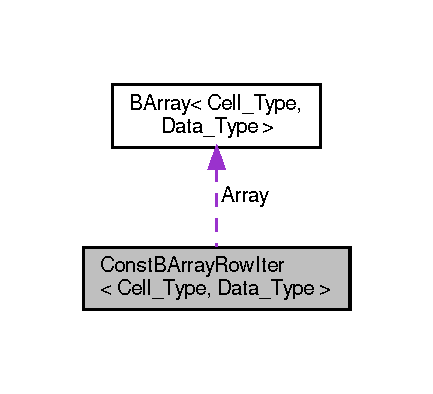
\includegraphics[width=208pt]{class_const_b_array_row_iter__coll__graph}
\end{center}
\end{figure}
\doxysubsection*{Public Member Functions}
\begin{DoxyCompactItemize}
\item 
\mbox{\hyperlink{class_const_b_array_row_iter_aa7eb0016052539d179dfe3fc82732f2e}{Const\+BArray\+Row\+Iter}} (\mbox{\hyperlink{barraydense-meat_8hpp_a92b303b76a3f942ea819498907d5e83c}{const}} \mbox{\hyperlink{class_b_array}{BArray}}$<$ Cell\+\_\+\+Type, Data\+\_\+\+Type $>$ $\ast$\mbox{\hyperlink{barray-meat_8hpp_a6cb31aaad809d508e214b61785d7fb47}{Array\+\_\+}})
\item 
\mbox{\hyperlink{class_const_b_array_row_iter_a5f32704679331be41e994d37294e3476}{$\sim$\+Const\+BArray\+Row\+Iter}} ()
\end{DoxyCompactItemize}
\doxysubsection*{Public Attributes}
\begin{DoxyCompactItemize}
\item 
size\+\_\+t \mbox{\hyperlink{class_const_b_array_row_iter_acc3a8aab1f5543d6074c7cca8f71aba3}{current\+\_\+row}}
\item 
size\+\_\+t \mbox{\hyperlink{class_const_b_array_row_iter_a10d542b63db8c099e34338f72c7e22ce}{current\+\_\+col}}
\item 
\mbox{\hyperlink{typedefs_8hpp_a84308a04a60581533b3c5e796c8248f5}{Row\+\_\+type}}$<$ Cell\+\_\+\+Type $>$\+::const\+\_\+iterator \mbox{\hyperlink{class_const_b_array_row_iter_ac01a8c0291ccc243bd4363bcbc5122a8}{iter}}
\item 
\mbox{\hyperlink{barraydense-meat_8hpp_a92b303b76a3f942ea819498907d5e83c}{const}} \mbox{\hyperlink{class_b_array}{BArray}}$<$ Cell\+\_\+\+Type, Data\+\_\+\+Type $>$ $\ast$ \mbox{\hyperlink{class_const_b_array_row_iter_ae7f5ef61225621953a664e73c6153ed3}{Array}}
\end{DoxyCompactItemize}


\doxysubsection{Detailed Description}
\subsubsection*{template$<$typename Cell\+\_\+\+Type, typename Data\+\_\+\+Type$>$\newline
class Const\+BArray\+Row\+Iter$<$ Cell\+\_\+\+Type, Data\+\_\+\+Type $>$}



Definition at line 10 of file barray-\/iterator.\+hpp.



\doxysubsection{Constructor \& Destructor Documentation}
\mbox{\Hypertarget{class_const_b_array_row_iter_aa7eb0016052539d179dfe3fc82732f2e}\label{class_const_b_array_row_iter_aa7eb0016052539d179dfe3fc82732f2e}} 
\index{ConstBArrayRowIter$<$ Cell\_Type, Data\_Type $>$@{ConstBArrayRowIter$<$ Cell\_Type, Data\_Type $>$}!ConstBArrayRowIter@{ConstBArrayRowIter}}
\index{ConstBArrayRowIter@{ConstBArrayRowIter}!ConstBArrayRowIter$<$ Cell\_Type, Data\_Type $>$@{ConstBArrayRowIter$<$ Cell\_Type, Data\_Type $>$}}
\doxysubsubsection{\texorpdfstring{ConstBArrayRowIter()}{ConstBArrayRowIter()}}
{\footnotesize\ttfamily template$<$typename Cell\+\_\+\+Type , typename Data\+\_\+\+Type $>$ \\
\mbox{\hyperlink{class_const_b_array_row_iter}{Const\+BArray\+Row\+Iter}}$<$ Cell\+\_\+\+Type, Data\+\_\+\+Type $>$\+::\mbox{\hyperlink{class_const_b_array_row_iter}{Const\+BArray\+Row\+Iter}} (\begin{DoxyParamCaption}\item[{\mbox{\hyperlink{barraydense-meat_8hpp_a92b303b76a3f942ea819498907d5e83c}{const}} \mbox{\hyperlink{class_b_array}{BArray}}$<$ Cell\+\_\+\+Type, Data\+\_\+\+Type $>$ $\ast$}]{Array\+\_\+ }\end{DoxyParamCaption})\hspace{0.3cm}{\ttfamily [inline]}}



Definition at line 17 of file barray-\/iterator.\+hpp.

\mbox{\Hypertarget{class_const_b_array_row_iter_a5f32704679331be41e994d37294e3476}\label{class_const_b_array_row_iter_a5f32704679331be41e994d37294e3476}} 
\index{ConstBArrayRowIter$<$ Cell\_Type, Data\_Type $>$@{ConstBArrayRowIter$<$ Cell\_Type, Data\_Type $>$}!````~ConstBArrayRowIter@{$\sim$ConstBArrayRowIter}}
\index{````~ConstBArrayRowIter@{$\sim$ConstBArrayRowIter}!ConstBArrayRowIter$<$ Cell\_Type, Data\_Type $>$@{ConstBArrayRowIter$<$ Cell\_Type, Data\_Type $>$}}
\doxysubsubsection{\texorpdfstring{$\sim$ConstBArrayRowIter()}{~ConstBArrayRowIter()}}
{\footnotesize\ttfamily template$<$typename Cell\+\_\+\+Type , typename Data\+\_\+\+Type $>$ \\
\mbox{\hyperlink{class_const_b_array_row_iter}{Const\+BArray\+Row\+Iter}}$<$ Cell\+\_\+\+Type, Data\+\_\+\+Type $>$\+::$\sim$\mbox{\hyperlink{class_const_b_array_row_iter}{Const\+BArray\+Row\+Iter}} (\begin{DoxyParamCaption}{ }\end{DoxyParamCaption})\hspace{0.3cm}{\ttfamily [inline]}}



Definition at line 29 of file barray-\/iterator.\+hpp.



\doxysubsection{Member Data Documentation}
\mbox{\Hypertarget{class_const_b_array_row_iter_ae7f5ef61225621953a664e73c6153ed3}\label{class_const_b_array_row_iter_ae7f5ef61225621953a664e73c6153ed3}} 
\index{ConstBArrayRowIter$<$ Cell\_Type, Data\_Type $>$@{ConstBArrayRowIter$<$ Cell\_Type, Data\_Type $>$}!Array@{Array}}
\index{Array@{Array}!ConstBArrayRowIter$<$ Cell\_Type, Data\_Type $>$@{ConstBArrayRowIter$<$ Cell\_Type, Data\_Type $>$}}
\doxysubsubsection{\texorpdfstring{Array}{Array}}
{\footnotesize\ttfamily template$<$typename Cell\+\_\+\+Type , typename Data\+\_\+\+Type $>$ \\
\mbox{\hyperlink{barraydense-meat_8hpp_a92b303b76a3f942ea819498907d5e83c}{const}} \mbox{\hyperlink{class_b_array}{BArray}}$<$Cell\+\_\+\+Type,Data\+\_\+\+Type$>$$\ast$ \mbox{\hyperlink{class_const_b_array_row_iter}{Const\+BArray\+Row\+Iter}}$<$ Cell\+\_\+\+Type, Data\+\_\+\+Type $>$\+::Array}



Definition at line 15 of file barray-\/iterator.\+hpp.

\mbox{\Hypertarget{class_const_b_array_row_iter_a10d542b63db8c099e34338f72c7e22ce}\label{class_const_b_array_row_iter_a10d542b63db8c099e34338f72c7e22ce}} 
\index{ConstBArrayRowIter$<$ Cell\_Type, Data\_Type $>$@{ConstBArrayRowIter$<$ Cell\_Type, Data\_Type $>$}!current\_col@{current\_col}}
\index{current\_col@{current\_col}!ConstBArrayRowIter$<$ Cell\_Type, Data\_Type $>$@{ConstBArrayRowIter$<$ Cell\_Type, Data\_Type $>$}}
\doxysubsubsection{\texorpdfstring{current\_col}{current\_col}}
{\footnotesize\ttfamily template$<$typename Cell\+\_\+\+Type , typename Data\+\_\+\+Type $>$ \\
size\+\_\+t \mbox{\hyperlink{class_const_b_array_row_iter}{Const\+BArray\+Row\+Iter}}$<$ Cell\+\_\+\+Type, Data\+\_\+\+Type $>$\+::current\+\_\+col}



Definition at line 13 of file barray-\/iterator.\+hpp.

\mbox{\Hypertarget{class_const_b_array_row_iter_acc3a8aab1f5543d6074c7cca8f71aba3}\label{class_const_b_array_row_iter_acc3a8aab1f5543d6074c7cca8f71aba3}} 
\index{ConstBArrayRowIter$<$ Cell\_Type, Data\_Type $>$@{ConstBArrayRowIter$<$ Cell\_Type, Data\_Type $>$}!current\_row@{current\_row}}
\index{current\_row@{current\_row}!ConstBArrayRowIter$<$ Cell\_Type, Data\_Type $>$@{ConstBArrayRowIter$<$ Cell\_Type, Data\_Type $>$}}
\doxysubsubsection{\texorpdfstring{current\_row}{current\_row}}
{\footnotesize\ttfamily template$<$typename Cell\+\_\+\+Type , typename Data\+\_\+\+Type $>$ \\
size\+\_\+t \mbox{\hyperlink{class_const_b_array_row_iter}{Const\+BArray\+Row\+Iter}}$<$ Cell\+\_\+\+Type, Data\+\_\+\+Type $>$\+::current\+\_\+row}



Definition at line 13 of file barray-\/iterator.\+hpp.

\mbox{\Hypertarget{class_const_b_array_row_iter_ac01a8c0291ccc243bd4363bcbc5122a8}\label{class_const_b_array_row_iter_ac01a8c0291ccc243bd4363bcbc5122a8}} 
\index{ConstBArrayRowIter$<$ Cell\_Type, Data\_Type $>$@{ConstBArrayRowIter$<$ Cell\_Type, Data\_Type $>$}!iter@{iter}}
\index{iter@{iter}!ConstBArrayRowIter$<$ Cell\_Type, Data\_Type $>$@{ConstBArrayRowIter$<$ Cell\_Type, Data\_Type $>$}}
\doxysubsubsection{\texorpdfstring{iter}{iter}}
{\footnotesize\ttfamily template$<$typename Cell\+\_\+\+Type , typename Data\+\_\+\+Type $>$ \\
\mbox{\hyperlink{typedefs_8hpp_a84308a04a60581533b3c5e796c8248f5}{Row\+\_\+type}}$<$Cell\+\_\+\+Type$>$\+::const\+\_\+iterator \mbox{\hyperlink{class_const_b_array_row_iter}{Const\+BArray\+Row\+Iter}}$<$ Cell\+\_\+\+Type, Data\+\_\+\+Type $>$\+::iter}



Definition at line 14 of file barray-\/iterator.\+hpp.



The documentation for this class was generated from the following file\+:\begin{DoxyCompactItemize}
\item 
include/barry/\mbox{\hyperlink{barray-iterator_8hpp}{barray-\/iterator.\+hpp}}\end{DoxyCompactItemize}

\hypertarget{classbarry_1_1_counter}{}\section{barry\+:\+:Counter$<$ Array\+\_\+\+Type, Data\+\_\+\+Type $>$ Class Template Reference}
\label{classbarry_1_1_counter}\index{barry\+::\+Counter$<$ Array\+\_\+\+Type, Data\+\_\+\+Type $>$@{barry\+::\+Counter$<$ Array\+\_\+\+Type, Data\+\_\+\+Type $>$}}


A counter function based on change statistics.  




{\ttfamily \#include $<$barry.\+hpp$>$}

\subsection*{Public Member Functions}
\begin{DoxyCompactItemize}
\item 
\hyperlink{classbarry_1_1_counter}{Counter}$<$ Array\+\_\+\+Type, Data\+\_\+\+Type $>$ \hyperlink{classbarry_1_1_counter_a058b8f695d6b6493c5d03aee8c01a86c}{operator=} (const \hyperlink{classbarry_1_1_counter}{Counter}$<$ Array\+\_\+\+Type, Data\+\_\+\+Type $>$ \&counter\+\_\+)
\item 
\hyperlink{classbarry_1_1_counter_ad899c3d55bb15e76ed7df05006e88b38}{$\sim$\+Counter} ()
\item 
double \hyperlink{classbarry_1_1_counter_a7b99fc45147d89c1b2db987e6b11f1f0}{count} (Array\+\_\+\+Type \&Array, \hyperlink{namespacebarry_a11dfc53ddb4672278319aa04f1e09a6c}{uint} i, \hyperlink{namespacebarry_a11dfc53ddb4672278319aa04f1e09a6c}{uint} j)
\item 
double \hyperlink{classbarry_1_1_counter_a835aa75876bc43a84ecbde4fd6a03fd5}{init} (Array\+\_\+\+Type \&Array, \hyperlink{namespacebarry_a11dfc53ddb4672278319aa04f1e09a6c}{uint} i, \hyperlink{namespacebarry_a11dfc53ddb4672278319aa04f1e09a6c}{uint} j)
\end{DoxyCompactItemize}
\begin{Indent}\textbf{ Creator passing a counter and an initializer}\par
{\em 
\begin{DoxyParams}{Parameters}
{\em count\+\_\+fun\+\_\+} & The main counter function. \\
\hline
{\em init\+\_\+fun\+\_\+} & The initializer function can also be used to check if the {\ttfamily \hyperlink{classbarry_1_1_b_array}{B\+Array}} as the needed variables (see \hyperlink{class_b_array_a9576163b52124021575e50dbcca2f6b9}{B\+Array\+::data}). \\
\hline
{\em data\+\_\+} & Data to be used with the counter. \\
\hline
{\em delete\+\_\+data\+\_\+} & When {\ttfamily true}, the destructor will delete the pointer in the main data. \\
\hline
\end{DoxyParams}
}\begin{DoxyCompactItemize}
\item 
\hyperlink{classbarry_1_1_counter_a3c990d6dbcdc553b3179c8353497a7df}{Counter} ()
\item 
\hyperlink{classbarry_1_1_counter_a1e886197c8f42b2552ada2786726fa38}{Counter} (\hyperlink{namespacebarry_a89b0a03ea2e7f83f2ae89be70a798337}{Counter\+\_\+fun\+\_\+type}$<$ Array\+\_\+\+Type, Data\+\_\+\+Type $>$ count\+\_\+fun\+\_\+, \hyperlink{namespacebarry_a89b0a03ea2e7f83f2ae89be70a798337}{Counter\+\_\+fun\+\_\+type}$<$ Array\+\_\+\+Type, Data\+\_\+\+Type $>$ init\+\_\+fun\+\_\+=nullptr, Data\+\_\+\+Type $\ast$data\+\_\+=nullptr, bool delete\+\_\+data\+\_\+=false)
\item 
\hyperlink{classbarry_1_1_counter_a89aa39dd007b8aa1bcde97519d516806}{Counter} (const \hyperlink{classbarry_1_1_counter}{Counter}$<$ Array\+\_\+\+Type, Data\+\_\+\+Type $>$ \&counter\+\_\+)
\end{DoxyCompactItemize}
\end{Indent}
\subsection*{Public Attributes}
\begin{DoxyCompactItemize}
\item 
\hyperlink{namespacebarry_a89b0a03ea2e7f83f2ae89be70a798337}{Counter\+\_\+fun\+\_\+type}$<$ Array\+\_\+\+Type, Data\+\_\+\+Type $>$ \hyperlink{classbarry_1_1_counter_aa535e164838a3a9c780e8d15fe45679b}{count\+\_\+fun}
\item 
\hyperlink{namespacebarry_a89b0a03ea2e7f83f2ae89be70a798337}{Counter\+\_\+fun\+\_\+type}$<$ Array\+\_\+\+Type, Data\+\_\+\+Type $>$ \hyperlink{classbarry_1_1_counter_a2509d75d3fc9e33d708911a38373d8ab}{init\+\_\+fun}
\item 
Data\+\_\+\+Type $\ast$ \hyperlink{classbarry_1_1_counter_af8196eeaaa4b58b788969c07aee7f1ee}{data} = nullptr
\item 
bool \hyperlink{classbarry_1_1_counter_a5445fa47abeff4b5675a5e5c12e4917a}{delete\+\_\+data} = false
\end{DoxyCompactItemize}


\subsection{Detailed Description}
\subsubsection*{template$<$typename Array\+\_\+\+Type = B\+Array$<$$>$, typename Data\+\_\+\+Type = bool$>$\newline
class barry\+::\+Counter$<$ Array\+\_\+\+Type, Data\+\_\+\+Type $>$}

A counter function based on change statistics. 

This class is used by {\ttfamily Count\+Stats} and {\ttfamily \hyperlink{classbarry_1_1_stats_counter}{Stats\+Counter}} as a way to count statistics using change statistics. 

Definition at line 122 of file barry.\+hpp.



\subsection{Constructor \& Destructor Documentation}
\mbox{\Hypertarget{classbarry_1_1_counter_a3c990d6dbcdc553b3179c8353497a7df}\label{classbarry_1_1_counter_a3c990d6dbcdc553b3179c8353497a7df}} 
\index{barry\+::\+Counter@{barry\+::\+Counter}!Counter@{Counter}}
\index{Counter@{Counter}!barry\+::\+Counter@{barry\+::\+Counter}}
\subsubsection{\texorpdfstring{Counter()}{Counter()}\hspace{0.1cm}{\footnotesize\ttfamily [1/3]}}
{\footnotesize\ttfamily template$<$typename Array\+\_\+\+Type  = B\+Array$<$$>$, typename Data\+\_\+\+Type  = bool$>$ \\
\hyperlink{classbarry_1_1_counter}{barry\+::\+Counter}$<$ Array\+\_\+\+Type, Data\+\_\+\+Type $>$\+::\hyperlink{classbarry_1_1_counter}{Counter} (\begin{DoxyParamCaption}{ }\end{DoxyParamCaption})\hspace{0.3cm}{\ttfamily [inline]}}



Definition at line 34 of file barry.\+hpp.

\mbox{\Hypertarget{classbarry_1_1_counter_a1e886197c8f42b2552ada2786726fa38}\label{classbarry_1_1_counter_a1e886197c8f42b2552ada2786726fa38}} 
\index{barry\+::\+Counter@{barry\+::\+Counter}!Counter@{Counter}}
\index{Counter@{Counter}!barry\+::\+Counter@{barry\+::\+Counter}}
\subsubsection{\texorpdfstring{Counter()}{Counter()}\hspace{0.1cm}{\footnotesize\ttfamily [2/3]}}
{\footnotesize\ttfamily template$<$typename Array\+\_\+\+Type  = B\+Array$<$$>$, typename Data\+\_\+\+Type  = bool$>$ \\
\hyperlink{classbarry_1_1_counter}{barry\+::\+Counter}$<$ Array\+\_\+\+Type, Data\+\_\+\+Type $>$\+::\hyperlink{classbarry_1_1_counter}{Counter} (\begin{DoxyParamCaption}\item[{\hyperlink{namespacebarry_a89b0a03ea2e7f83f2ae89be70a798337}{Counter\+\_\+fun\+\_\+type}$<$ Array\+\_\+\+Type, Data\+\_\+\+Type $>$}]{count\+\_\+fun\+\_\+,  }\item[{\hyperlink{namespacebarry_a89b0a03ea2e7f83f2ae89be70a798337}{Counter\+\_\+fun\+\_\+type}$<$ Array\+\_\+\+Type, Data\+\_\+\+Type $>$}]{init\+\_\+fun\+\_\+ = {\ttfamily nullptr},  }\item[{Data\+\_\+\+Type $\ast$}]{data\+\_\+ = {\ttfamily nullptr},  }\item[{bool}]{delete\+\_\+data\+\_\+ = {\ttfamily false} }\end{DoxyParamCaption})\hspace{0.3cm}{\ttfamily [inline]}}



Definition at line 36 of file barry.\+hpp.

\mbox{\Hypertarget{classbarry_1_1_counter_a89aa39dd007b8aa1bcde97519d516806}\label{classbarry_1_1_counter_a89aa39dd007b8aa1bcde97519d516806}} 
\index{barry\+::\+Counter@{barry\+::\+Counter}!Counter@{Counter}}
\index{Counter@{Counter}!barry\+::\+Counter@{barry\+::\+Counter}}
\subsubsection{\texorpdfstring{Counter()}{Counter()}\hspace{0.1cm}{\footnotesize\ttfamily [3/3]}}
{\footnotesize\ttfamily template$<$typename Array\+\_\+\+Type , typename Data\+\_\+\+Type $>$ \\
\hyperlink{classbarry_1_1_counter}{Counter}$<$ Array\+\_\+\+Type, Data\+\_\+\+Type $>$\+::\hyperlink{classbarry_1_1_counter}{Counter} (\begin{DoxyParamCaption}\item[{const \hyperlink{classbarry_1_1_counter}{Counter}$<$ Array\+\_\+\+Type, Data\+\_\+\+Type $>$ \&}]{counter\+\_\+ }\end{DoxyParamCaption})\hspace{0.3cm}{\ttfamily [inline]}}



Definition at line 7 of file barry.\+hpp.

\mbox{\Hypertarget{classbarry_1_1_counter_ad899c3d55bb15e76ed7df05006e88b38}\label{classbarry_1_1_counter_ad899c3d55bb15e76ed7df05006e88b38}} 
\index{barry\+::\+Counter@{barry\+::\+Counter}!````~Counter@{$\sim$\+Counter}}
\index{````~Counter@{$\sim$\+Counter}!barry\+::\+Counter@{barry\+::\+Counter}}
\subsubsection{\texorpdfstring{$\sim$\+Counter()}{~Counter()}}
{\footnotesize\ttfamily template$<$typename Array\+\_\+\+Type  = B\+Array$<$$>$, typename Data\+\_\+\+Type  = bool$>$ \\
\hyperlink{classbarry_1_1_counter}{barry\+::\+Counter}$<$ Array\+\_\+\+Type, Data\+\_\+\+Type $>$\+::$\sim$\hyperlink{classbarry_1_1_counter}{Counter} (\begin{DoxyParamCaption}{ }\end{DoxyParamCaption})\hspace{0.3cm}{\ttfamily [inline]}}



Definition at line 48 of file barry.\+hpp.



\subsection{Member Function Documentation}
\mbox{\Hypertarget{classbarry_1_1_counter_a7b99fc45147d89c1b2db987e6b11f1f0}\label{classbarry_1_1_counter_a7b99fc45147d89c1b2db987e6b11f1f0}} 
\index{barry\+::\+Counter@{barry\+::\+Counter}!count@{count}}
\index{count@{count}!barry\+::\+Counter@{barry\+::\+Counter}}
\subsubsection{\texorpdfstring{count()}{count()}}
{\footnotesize\ttfamily template$<$typename Array\+\_\+\+Type , typename Data\+\_\+\+Type $>$ \\
double \hyperlink{classbarry_1_1_counter}{Counter}$<$ Array\+\_\+\+Type, Data\+\_\+\+Type $>$\+::count (\begin{DoxyParamCaption}\item[{Array\+\_\+\+Type \&}]{Array,  }\item[{\hyperlink{namespacebarry_a11dfc53ddb4672278319aa04f1e09a6c}{uint}}]{i,  }\item[{\hyperlink{namespacebarry_a11dfc53ddb4672278319aa04f1e09a6c}{uint}}]{j }\end{DoxyParamCaption})\hspace{0.3cm}{\ttfamily [inline]}}



Definition at line 100 of file barry.\+hpp.

\mbox{\Hypertarget{classbarry_1_1_counter_a835aa75876bc43a84ecbde4fd6a03fd5}\label{classbarry_1_1_counter_a835aa75876bc43a84ecbde4fd6a03fd5}} 
\index{barry\+::\+Counter@{barry\+::\+Counter}!init@{init}}
\index{init@{init}!barry\+::\+Counter@{barry\+::\+Counter}}
\subsubsection{\texorpdfstring{init()}{init()}}
{\footnotesize\ttfamily template$<$typename Array\+\_\+\+Type , typename Data\+\_\+\+Type $>$ \\
double \hyperlink{classbarry_1_1_counter}{Counter}$<$ Array\+\_\+\+Type, Data\+\_\+\+Type $>$\+::init (\begin{DoxyParamCaption}\item[{Array\+\_\+\+Type \&}]{Array,  }\item[{\hyperlink{namespacebarry_a11dfc53ddb4672278319aa04f1e09a6c}{uint}}]{i,  }\item[{\hyperlink{namespacebarry_a11dfc53ddb4672278319aa04f1e09a6c}{uint}}]{j }\end{DoxyParamCaption})\hspace{0.3cm}{\ttfamily [inline]}}



Definition at line 108 of file barry.\+hpp.

\mbox{\Hypertarget{classbarry_1_1_counter_a058b8f695d6b6493c5d03aee8c01a86c}\label{classbarry_1_1_counter_a058b8f695d6b6493c5d03aee8c01a86c}} 
\index{barry\+::\+Counter@{barry\+::\+Counter}!operator=@{operator=}}
\index{operator=@{operator=}!barry\+::\+Counter@{barry\+::\+Counter}}
\subsubsection{\texorpdfstring{operator=()}{operator=()}}
{\footnotesize\ttfamily template$<$typename Array\+\_\+\+Type , typename Data\+\_\+\+Type $>$ \\
\hyperlink{classbarry_1_1_counter}{Counter}$<$ Array\+\_\+\+Type, Data\+\_\+\+Type $>$ \hyperlink{classbarry_1_1_counter}{Counter}$<$ Array\+\_\+\+Type, Data\+\_\+\+Type $>$\+::operator= (\begin{DoxyParamCaption}\item[{const \hyperlink{classbarry_1_1_counter}{Counter}$<$ Array\+\_\+\+Type, Data\+\_\+\+Type $>$ \&}]{counter\+\_\+ }\end{DoxyParamCaption})}



Definition at line 24 of file barry.\+hpp.



\subsection{Member Data Documentation}
\mbox{\Hypertarget{classbarry_1_1_counter_aa535e164838a3a9c780e8d15fe45679b}\label{classbarry_1_1_counter_aa535e164838a3a9c780e8d15fe45679b}} 
\index{barry\+::\+Counter@{barry\+::\+Counter}!count\+\_\+fun@{count\+\_\+fun}}
\index{count\+\_\+fun@{count\+\_\+fun}!barry\+::\+Counter@{barry\+::\+Counter}}
\subsubsection{\texorpdfstring{count\+\_\+fun}{count\_fun}}
{\footnotesize\ttfamily template$<$typename Array\+\_\+\+Type  = B\+Array$<$$>$, typename Data\+\_\+\+Type  = bool$>$ \\
\hyperlink{namespacebarry_a89b0a03ea2e7f83f2ae89be70a798337}{Counter\+\_\+fun\+\_\+type}$<$Array\+\_\+\+Type,Data\+\_\+\+Type$>$ \hyperlink{classbarry_1_1_counter}{barry\+::\+Counter}$<$ Array\+\_\+\+Type, Data\+\_\+\+Type $>$\+::count\+\_\+fun}



Definition at line 18 of file barry.\+hpp.

\mbox{\Hypertarget{classbarry_1_1_counter_af8196eeaaa4b58b788969c07aee7f1ee}\label{classbarry_1_1_counter_af8196eeaaa4b58b788969c07aee7f1ee}} 
\index{barry\+::\+Counter@{barry\+::\+Counter}!data@{data}}
\index{data@{data}!barry\+::\+Counter@{barry\+::\+Counter}}
\subsubsection{\texorpdfstring{data}{data}}
{\footnotesize\ttfamily template$<$typename Array\+\_\+\+Type  = B\+Array$<$$>$, typename Data\+\_\+\+Type  = bool$>$ \\
Data\+\_\+\+Type$\ast$ \hyperlink{classbarry_1_1_counter}{barry\+::\+Counter}$<$ Array\+\_\+\+Type, Data\+\_\+\+Type $>$\+::data = nullptr}



Definition at line 20 of file barry.\+hpp.

\mbox{\Hypertarget{classbarry_1_1_counter_a5445fa47abeff4b5675a5e5c12e4917a}\label{classbarry_1_1_counter_a5445fa47abeff4b5675a5e5c12e4917a}} 
\index{barry\+::\+Counter@{barry\+::\+Counter}!delete\+\_\+data@{delete\+\_\+data}}
\index{delete\+\_\+data@{delete\+\_\+data}!barry\+::\+Counter@{barry\+::\+Counter}}
\subsubsection{\texorpdfstring{delete\+\_\+data}{delete\_data}}
{\footnotesize\ttfamily template$<$typename Array\+\_\+\+Type  = B\+Array$<$$>$, typename Data\+\_\+\+Type  = bool$>$ \\
bool \hyperlink{classbarry_1_1_counter}{barry\+::\+Counter}$<$ Array\+\_\+\+Type, Data\+\_\+\+Type $>$\+::delete\+\_\+data = false}



Definition at line 21 of file barry.\+hpp.

\mbox{\Hypertarget{classbarry_1_1_counter_a2509d75d3fc9e33d708911a38373d8ab}\label{classbarry_1_1_counter_a2509d75d3fc9e33d708911a38373d8ab}} 
\index{barry\+::\+Counter@{barry\+::\+Counter}!init\+\_\+fun@{init\+\_\+fun}}
\index{init\+\_\+fun@{init\+\_\+fun}!barry\+::\+Counter@{barry\+::\+Counter}}
\subsubsection{\texorpdfstring{init\+\_\+fun}{init\_fun}}
{\footnotesize\ttfamily template$<$typename Array\+\_\+\+Type  = B\+Array$<$$>$, typename Data\+\_\+\+Type  = bool$>$ \\
\hyperlink{namespacebarry_a89b0a03ea2e7f83f2ae89be70a798337}{Counter\+\_\+fun\+\_\+type}$<$Array\+\_\+\+Type,Data\+\_\+\+Type$>$ \hyperlink{classbarry_1_1_counter}{barry\+::\+Counter}$<$ Array\+\_\+\+Type, Data\+\_\+\+Type $>$\+::init\+\_\+fun}



Definition at line 19 of file barry.\+hpp.



The documentation for this class was generated from the following file\+:\begin{DoxyCompactItemize}
\item 
include/barry/\hyperlink{barry_8hpp}{barry.\+hpp}\end{DoxyCompactItemize}

\hypertarget{class_counter}{}\section{Counter$<$ Array\+\_\+\+Type, Data\+\_\+\+Type $>$ Class Template Reference}
\label{class_counter}\index{Counter$<$ Array\+\_\+\+Type, Data\+\_\+\+Type $>$@{Counter$<$ Array\+\_\+\+Type, Data\+\_\+\+Type $>$}}


A counter function based on change statistics.  




{\ttfamily \#include $<$counters-\/bones.\+hpp$>$}

\subsection*{Public Member Functions}
\begin{DoxyCompactItemize}
\item 
\hyperlink{class_counter_a56c2f4ad875497dea97934cd3ddebc81}{Counter} ()
\item 
\hyperlink{class_counter_ad2a63c2b9b6c593d292dfd47e2f7a780}{Counter} (\hyperlink{typedefs_8hpp_ac0160f52f564dea3ac033b374cffbfe7}{Counter\+\_\+fun\+\_\+type}$<$ Array\+\_\+\+Type, Data\+\_\+\+Type $>$ count\+\_\+fun\+\_\+, \hyperlink{typedefs_8hpp_ac0160f52f564dea3ac033b374cffbfe7}{Counter\+\_\+fun\+\_\+type}$<$ Array\+\_\+\+Type, Data\+\_\+\+Type $>$ init\+\_\+fun\+\_\+=nullptr, Data\+\_\+\+Type $\ast$data\+\_\+=nullptr, bool delete\+\_\+data\+\_\+=false)
\begin{DoxyCompactList}\small\item\em Creator passing a counter and an initializer. \end{DoxyCompactList}\item 
\hyperlink{class_counter_a89aa39dd007b8aa1bcde97519d516806}{Counter} (const \hyperlink{class_counter}{Counter}$<$ Array\+\_\+\+Type, Data\+\_\+\+Type $>$ \&counter\+\_\+)
\item 
\hyperlink{class_counter}{Counter}$<$ Array\+\_\+\+Type, Data\+\_\+\+Type $>$ \hyperlink{class_counter_a058b8f695d6b6493c5d03aee8c01a86c}{operator=} (const \hyperlink{class_counter}{Counter}$<$ Array\+\_\+\+Type, Data\+\_\+\+Type $>$ \&counter\+\_\+)
\item 
\hyperlink{class_counter_a66594b4ffbbf337241b032c1f039b3c0}{$\sim$\+Counter} ()
\item 
double \hyperlink{class_counter_afe1d23e72c3bdca9b2481f36ebde1d95}{count} (Array\+\_\+\+Type $\ast$Array, \hyperlink{typedefs_8hpp_a91ad9478d81a7aaf2593e8d9c3d06a14}{uint} i, \hyperlink{typedefs_8hpp_a91ad9478d81a7aaf2593e8d9c3d06a14}{uint} j)
\item 
double \hyperlink{class_counter_ae0451979ddc51a5fbf00de78c37d3216}{init} (Array\+\_\+\+Type $\ast$Array, \hyperlink{typedefs_8hpp_a91ad9478d81a7aaf2593e8d9c3d06a14}{uint} i, \hyperlink{typedefs_8hpp_a91ad9478d81a7aaf2593e8d9c3d06a14}{uint} j)
\end{DoxyCompactItemize}
\subsection*{Public Attributes}
\begin{DoxyCompactItemize}
\item 
\hyperlink{typedefs_8hpp_ac0160f52f564dea3ac033b374cffbfe7}{Counter\+\_\+fun\+\_\+type}$<$ Array\+\_\+\+Type, Data\+\_\+\+Type $>$ \hyperlink{class_counter_a804d287379ef9b4204a0838edcce3b71}{count\+\_\+fun}
\item 
\hyperlink{typedefs_8hpp_ac0160f52f564dea3ac033b374cffbfe7}{Counter\+\_\+fun\+\_\+type}$<$ Array\+\_\+\+Type, Data\+\_\+\+Type $>$ \hyperlink{class_counter_abb4e0b67e6489d438918495651baa5a8}{init\+\_\+fun}
\item 
Data\+\_\+\+Type $\ast$ \hyperlink{class_counter_a9ebfed99a67888f80c19cabc4098bdd0}{data} = nullptr
\item 
bool \hyperlink{class_counter_a5190fbe81aac2426ac36c0a088e242e7}{delete\+\_\+data} = false
\end{DoxyCompactItemize}


\subsection{Detailed Description}
\subsubsection*{template$<$typename Array\+\_\+\+Type = B\+Array$<$$>$, typename Data\+\_\+\+Type = bool$>$\newline
class Counter$<$ Array\+\_\+\+Type, Data\+\_\+\+Type $>$}

A counter function based on change statistics. 

This class is used by {\ttfamily Count\+Stats} and {\ttfamily \hyperlink{class_stats_counter}{Stats\+Counter}} as a way to count statistics using change statistics. 

Definition at line 15 of file counters-\/bones.\+hpp.



\subsection{Constructor \& Destructor Documentation}
\mbox{\Hypertarget{class_counter_a56c2f4ad875497dea97934cd3ddebc81}\label{class_counter_a56c2f4ad875497dea97934cd3ddebc81}} 
\index{Counter@{Counter}!Counter@{Counter}}
\index{Counter@{Counter}!Counter@{Counter}}
\subsubsection{\texorpdfstring{Counter()}{Counter()}\hspace{0.1cm}{\footnotesize\ttfamily [1/3]}}
{\footnotesize\ttfamily template$<$typename Array\+\_\+\+Type = B\+Array$<$$>$, typename Data\+\_\+\+Type = bool$>$ \\
\hyperlink{class_counter}{Counter}$<$ Array\+\_\+\+Type, Data\+\_\+\+Type $>$\+::\hyperlink{class_counter}{Counter} (\begin{DoxyParamCaption}{ }\end{DoxyParamCaption})\hspace{0.3cm}{\ttfamily [inline]}}



Definition at line 26 of file counters-\/bones.\+hpp.

\mbox{\Hypertarget{class_counter_ad2a63c2b9b6c593d292dfd47e2f7a780}\label{class_counter_ad2a63c2b9b6c593d292dfd47e2f7a780}} 
\index{Counter@{Counter}!Counter@{Counter}}
\index{Counter@{Counter}!Counter@{Counter}}
\subsubsection{\texorpdfstring{Counter()}{Counter()}\hspace{0.1cm}{\footnotesize\ttfamily [2/3]}}
{\footnotesize\ttfamily template$<$typename Array\+\_\+\+Type = B\+Array$<$$>$, typename Data\+\_\+\+Type = bool$>$ \\
\hyperlink{class_counter}{Counter}$<$ Array\+\_\+\+Type, Data\+\_\+\+Type $>$\+::\hyperlink{class_counter}{Counter} (\begin{DoxyParamCaption}\item[{\hyperlink{typedefs_8hpp_ac0160f52f564dea3ac033b374cffbfe7}{Counter\+\_\+fun\+\_\+type}$<$ Array\+\_\+\+Type, Data\+\_\+\+Type $>$}]{count\+\_\+fun\+\_\+,  }\item[{\hyperlink{typedefs_8hpp_ac0160f52f564dea3ac033b374cffbfe7}{Counter\+\_\+fun\+\_\+type}$<$ Array\+\_\+\+Type, Data\+\_\+\+Type $>$}]{init\+\_\+fun\+\_\+ = {\ttfamily nullptr},  }\item[{Data\+\_\+\+Type $\ast$}]{data\+\_\+ = {\ttfamily nullptr},  }\item[{bool}]{delete\+\_\+data\+\_\+ = {\ttfamily false} }\end{DoxyParamCaption})\hspace{0.3cm}{\ttfamily [inline]}}



Creator passing a counter and an initializer. 


\begin{DoxyParams}{Parameters}
{\em count\+\_\+fun\+\_\+} & The main counter function. \\
\hline
{\em init\+\_\+fun\+\_\+} & The initializer function can also be used to check if the {\ttfamily \hyperlink{class_b_array}{B\+Array}} as the needed variables (see \hyperlink{class_b_array_a9576163b52124021575e50dbcca2f6b9}{B\+Array\+::data}). \\
\hline
{\em data\+\_\+} & Data to be used with the counter. \\
\hline
{\em delete\+\_\+data\+\_\+} & When {\ttfamily true}, the destructor will delete the pointer in the main data. \\
\hline
\end{DoxyParams}


Definition at line 38 of file counters-\/bones.\+hpp.

\mbox{\Hypertarget{class_counter_a89aa39dd007b8aa1bcde97519d516806}\label{class_counter_a89aa39dd007b8aa1bcde97519d516806}} 
\index{Counter@{Counter}!Counter@{Counter}}
\index{Counter@{Counter}!Counter@{Counter}}
\subsubsection{\texorpdfstring{Counter()}{Counter()}\hspace{0.1cm}{\footnotesize\ttfamily [3/3]}}
{\footnotesize\ttfamily template$<$typename Array\+\_\+\+Type , typename Data\+\_\+\+Type $>$ \\
\hyperlink{class_counter}{Counter}$<$ Array\+\_\+\+Type, Data\+\_\+\+Type $>$\+::\hyperlink{class_counter}{Counter} (\begin{DoxyParamCaption}\item[{const \hyperlink{class_counter}{Counter}$<$ Array\+\_\+\+Type, Data\+\_\+\+Type $>$ \&}]{counter\+\_\+ }\end{DoxyParamCaption})\hspace{0.3cm}{\ttfamily [inline]}}



Definition at line 7 of file counters-\/meat.\+hpp.

\mbox{\Hypertarget{class_counter_a66594b4ffbbf337241b032c1f039b3c0}\label{class_counter_a66594b4ffbbf337241b032c1f039b3c0}} 
\index{Counter@{Counter}!````~Counter@{$\sim$\+Counter}}
\index{````~Counter@{$\sim$\+Counter}!Counter@{Counter}}
\subsubsection{\texorpdfstring{$\sim$\+Counter()}{~Counter()}}
{\footnotesize\ttfamily template$<$typename Array\+\_\+\+Type = B\+Array$<$$>$, typename Data\+\_\+\+Type = bool$>$ \\
\hyperlink{class_counter}{Counter}$<$ Array\+\_\+\+Type, Data\+\_\+\+Type $>$\+::$\sim$\hyperlink{class_counter}{Counter} (\begin{DoxyParamCaption}{ }\end{DoxyParamCaption})\hspace{0.3cm}{\ttfamily [inline]}}



Definition at line 48 of file counters-\/bones.\+hpp.



\subsection{Member Function Documentation}
\mbox{\Hypertarget{class_counter_afe1d23e72c3bdca9b2481f36ebde1d95}\label{class_counter_afe1d23e72c3bdca9b2481f36ebde1d95}} 
\index{Counter@{Counter}!count@{count}}
\index{count@{count}!Counter@{Counter}}
\subsubsection{\texorpdfstring{count()}{count()}}
{\footnotesize\ttfamily template$<$typename Array\+\_\+\+Type , typename Data\+\_\+\+Type $>$ \\
double \hyperlink{class_counter}{Counter}$<$ Array\+\_\+\+Type, Data\+\_\+\+Type $>$\+::count (\begin{DoxyParamCaption}\item[{Array\+\_\+\+Type $\ast$}]{Array,  }\item[{\hyperlink{typedefs_8hpp_a91ad9478d81a7aaf2593e8d9c3d06a14}{uint}}]{i,  }\item[{\hyperlink{typedefs_8hpp_a91ad9478d81a7aaf2593e8d9c3d06a14}{uint}}]{j }\end{DoxyParamCaption})\hspace{0.3cm}{\ttfamily [inline]}}



Definition at line 100 of file counters-\/meat.\+hpp.

\mbox{\Hypertarget{class_counter_ae0451979ddc51a5fbf00de78c37d3216}\label{class_counter_ae0451979ddc51a5fbf00de78c37d3216}} 
\index{Counter@{Counter}!init@{init}}
\index{init@{init}!Counter@{Counter}}
\subsubsection{\texorpdfstring{init()}{init()}}
{\footnotesize\ttfamily template$<$typename Array\+\_\+\+Type , typename Data\+\_\+\+Type $>$ \\
double \hyperlink{class_counter}{Counter}$<$ Array\+\_\+\+Type, Data\+\_\+\+Type $>$\+::init (\begin{DoxyParamCaption}\item[{Array\+\_\+\+Type $\ast$}]{Array,  }\item[{\hyperlink{typedefs_8hpp_a91ad9478d81a7aaf2593e8d9c3d06a14}{uint}}]{i,  }\item[{\hyperlink{typedefs_8hpp_a91ad9478d81a7aaf2593e8d9c3d06a14}{uint}}]{j }\end{DoxyParamCaption})\hspace{0.3cm}{\ttfamily [inline]}}



Definition at line 108 of file counters-\/meat.\+hpp.

\mbox{\Hypertarget{class_counter_a058b8f695d6b6493c5d03aee8c01a86c}\label{class_counter_a058b8f695d6b6493c5d03aee8c01a86c}} 
\index{Counter@{Counter}!operator=@{operator=}}
\index{operator=@{operator=}!Counter@{Counter}}
\subsubsection{\texorpdfstring{operator=()}{operator=()}}
{\footnotesize\ttfamily template$<$typename Array\+\_\+\+Type , typename Data\+\_\+\+Type $>$ \\
\hyperlink{class_counter}{Counter}$<$ Array\+\_\+\+Type, Data\+\_\+\+Type $>$ \hyperlink{class_counter}{Counter}$<$ Array\+\_\+\+Type, Data\+\_\+\+Type $>$\+::operator= (\begin{DoxyParamCaption}\item[{const \hyperlink{class_counter}{Counter}$<$ Array\+\_\+\+Type, Data\+\_\+\+Type $>$ \&}]{counter\+\_\+ }\end{DoxyParamCaption})}



Definition at line 24 of file counters-\/meat.\+hpp.



\subsection{Member Data Documentation}
\mbox{\Hypertarget{class_counter_a804d287379ef9b4204a0838edcce3b71}\label{class_counter_a804d287379ef9b4204a0838edcce3b71}} 
\index{Counter@{Counter}!count\+\_\+fun@{count\+\_\+fun}}
\index{count\+\_\+fun@{count\+\_\+fun}!Counter@{Counter}}
\subsubsection{\texorpdfstring{count\+\_\+fun}{count\_fun}}
{\footnotesize\ttfamily template$<$typename Array\+\_\+\+Type = B\+Array$<$$>$, typename Data\+\_\+\+Type = bool$>$ \\
\hyperlink{typedefs_8hpp_ac0160f52f564dea3ac033b374cffbfe7}{Counter\+\_\+fun\+\_\+type}$<$Array\+\_\+\+Type,Data\+\_\+\+Type$>$ \hyperlink{class_counter}{Counter}$<$ Array\+\_\+\+Type, Data\+\_\+\+Type $>$\+::count\+\_\+fun}



Definition at line 18 of file counters-\/bones.\+hpp.

\mbox{\Hypertarget{class_counter_a9ebfed99a67888f80c19cabc4098bdd0}\label{class_counter_a9ebfed99a67888f80c19cabc4098bdd0}} 
\index{Counter@{Counter}!data@{data}}
\index{data@{data}!Counter@{Counter}}
\subsubsection{\texorpdfstring{data}{data}}
{\footnotesize\ttfamily template$<$typename Array\+\_\+\+Type = B\+Array$<$$>$, typename Data\+\_\+\+Type = bool$>$ \\
Data\+\_\+\+Type$\ast$ \hyperlink{class_counter}{Counter}$<$ Array\+\_\+\+Type, Data\+\_\+\+Type $>$\+::data = nullptr}



Definition at line 20 of file counters-\/bones.\+hpp.

\mbox{\Hypertarget{class_counter_a5190fbe81aac2426ac36c0a088e242e7}\label{class_counter_a5190fbe81aac2426ac36c0a088e242e7}} 
\index{Counter@{Counter}!delete\+\_\+data@{delete\+\_\+data}}
\index{delete\+\_\+data@{delete\+\_\+data}!Counter@{Counter}}
\subsubsection{\texorpdfstring{delete\+\_\+data}{delete\_data}}
{\footnotesize\ttfamily template$<$typename Array\+\_\+\+Type = B\+Array$<$$>$, typename Data\+\_\+\+Type = bool$>$ \\
bool \hyperlink{class_counter}{Counter}$<$ Array\+\_\+\+Type, Data\+\_\+\+Type $>$\+::delete\+\_\+data = false}



Definition at line 21 of file counters-\/bones.\+hpp.

\mbox{\Hypertarget{class_counter_abb4e0b67e6489d438918495651baa5a8}\label{class_counter_abb4e0b67e6489d438918495651baa5a8}} 
\index{Counter@{Counter}!init\+\_\+fun@{init\+\_\+fun}}
\index{init\+\_\+fun@{init\+\_\+fun}!Counter@{Counter}}
\subsubsection{\texorpdfstring{init\+\_\+fun}{init\_fun}}
{\footnotesize\ttfamily template$<$typename Array\+\_\+\+Type = B\+Array$<$$>$, typename Data\+\_\+\+Type = bool$>$ \\
\hyperlink{typedefs_8hpp_ac0160f52f564dea3ac033b374cffbfe7}{Counter\+\_\+fun\+\_\+type}$<$Array\+\_\+\+Type,Data\+\_\+\+Type$>$ \hyperlink{class_counter}{Counter}$<$ Array\+\_\+\+Type, Data\+\_\+\+Type $>$\+::init\+\_\+fun}



Definition at line 19 of file counters-\/bones.\+hpp.



The documentation for this class was generated from the following files\+:\begin{DoxyCompactItemize}
\item 
include/barry/\hyperlink{counters-bones_8hpp}{counters-\/bones.\+hpp}\item 
include/barry/\hyperlink{counters-meat_8hpp}{counters-\/meat.\+hpp}\end{DoxyCompactItemize}

\hypertarget{classbarry_1_1_counter_vector}{}\section{barry\+:\+:Counter\+Vector$<$ Array\+\_\+\+Type, Data\+\_\+\+Type $>$ Class Template Reference}
\label{classbarry_1_1_counter_vector}\index{barry\+::\+Counter\+Vector$<$ Array\+\_\+\+Type, Data\+\_\+\+Type $>$@{barry\+::\+Counter\+Vector$<$ Array\+\_\+\+Type, Data\+\_\+\+Type $>$}}


Vector of counters.  




{\ttfamily \#include $<$barry.\+hpp$>$}

\subsection*{Public Member Functions}
\begin{DoxyCompactItemize}
\item 
\hyperlink{classbarry_1_1_counter_vector_a620e7a96ebfd05fe71da6476f27c2850}{Counter\+Vector} ()
\item 
\hyperlink{classbarry_1_1_counter_vector_a6a6cfc7b9a3ff220311d312786a8e3eb}{$\sim$\+Counter\+Vector} ()
\item 
\hyperlink{classbarry_1_1_counter}{Counter}$<$ Array\+\_\+\+Type, Data\+\_\+\+Type $>$ $\ast$ \hyperlink{classbarry_1_1_counter_vector_a6eac3e73298e1e6d424b92f324ffe9a8}{operator\mbox{[}$\,$\mbox{]}} (\hyperlink{namespacebarry_a11dfc53ddb4672278319aa04f1e09a6c}{uint} idx)
\item 
\hyperlink{namespacebarry_a11dfc53ddb4672278319aa04f1e09a6c}{uint} \hyperlink{classbarry_1_1_counter_vector_a05508f97e15d5a6dd2fdefb2d03060de}{size} () const
\item 
void \hyperlink{classbarry_1_1_counter_vector_a34fda06ff678691daf3b0455c1a2af48}{add\+\_\+counter} (\hyperlink{classbarry_1_1_counter}{Counter}$<$ Array\+\_\+\+Type, Data\+\_\+\+Type $>$ \&counter)
\item 
void \hyperlink{classbarry_1_1_counter_vector_a062d52e18f1d3ba4c00cbf4c2d89f1e7}{add\+\_\+counter} (\hyperlink{classbarry_1_1_counter}{Counter}$<$ Array\+\_\+\+Type, Data\+\_\+\+Type $>$ $\ast$counter)
\item 
void \hyperlink{classbarry_1_1_counter_vector_adb32ff1af45bc05a292a5cb064dc414d}{add\+\_\+counter} (\hyperlink{namespacebarry_abaaae3200da8e4b7faac3c04fe9c3081}{Counter\+\_\+fun\+\_\+type}$<$ Array\+\_\+\+Type, Data\+\_\+\+Type $>$ count\+\_\+fun\+\_\+, \hyperlink{namespacebarry_abaaae3200da8e4b7faac3c04fe9c3081}{Counter\+\_\+fun\+\_\+type}$<$ Array\+\_\+\+Type, Data\+\_\+\+Type $>$ init\+\_\+fun\+\_\+=nullptr, Data\+\_\+\+Type $\ast$data\+\_\+=nullptr, bool delete\+\_\+data\+\_\+=false)
\item 
void \hyperlink{classbarry_1_1_counter_vector_acce75748f917e3a7898d49a23df996e7}{clear} ()
\end{DoxyCompactItemize}


\subsection{Detailed Description}
\subsubsection*{template$<$typename Array\+\_\+\+Type = B\+Array$<$$>$, typename Data\+\_\+\+Type = bool$>$\newline
class barry\+::\+Counter\+Vector$<$ Array\+\_\+\+Type, Data\+\_\+\+Type $>$}

Vector of counters. 

Various functions hold more than one counter, so this class is a helper class that allows managing multiple counters efficiently. The main data is a vector to pointers of counters. 

Definition at line 84 of file barry.\+hpp.



\subsection{Constructor \& Destructor Documentation}
\mbox{\Hypertarget{classbarry_1_1_counter_vector_a620e7a96ebfd05fe71da6476f27c2850}\label{classbarry_1_1_counter_vector_a620e7a96ebfd05fe71da6476f27c2850}} 
\index{barry\+::\+Counter\+Vector@{barry\+::\+Counter\+Vector}!Counter\+Vector@{Counter\+Vector}}
\index{Counter\+Vector@{Counter\+Vector}!barry\+::\+Counter\+Vector@{barry\+::\+Counter\+Vector}}
\subsubsection{\texorpdfstring{Counter\+Vector()}{CounterVector()}}
{\footnotesize\ttfamily template$<$typename Array\+\_\+\+Type  = B\+Array$<$$>$, typename Data\+\_\+\+Type  = bool$>$ \\
\hyperlink{classbarry_1_1_counter_vector}{barry\+::\+Counter\+Vector}$<$ Array\+\_\+\+Type, Data\+\_\+\+Type $>$\+::\hyperlink{classbarry_1_1_counter_vector}{Counter\+Vector} (\begin{DoxyParamCaption}{ }\end{DoxyParamCaption})\hspace{0.3cm}{\ttfamily [inline]}}



Definition at line 93 of file barry.\+hpp.

\mbox{\Hypertarget{classbarry_1_1_counter_vector_a6a6cfc7b9a3ff220311d312786a8e3eb}\label{classbarry_1_1_counter_vector_a6a6cfc7b9a3ff220311d312786a8e3eb}} 
\index{barry\+::\+Counter\+Vector@{barry\+::\+Counter\+Vector}!````~Counter\+Vector@{$\sim$\+Counter\+Vector}}
\index{````~Counter\+Vector@{$\sim$\+Counter\+Vector}!barry\+::\+Counter\+Vector@{barry\+::\+Counter\+Vector}}
\subsubsection{\texorpdfstring{$\sim$\+Counter\+Vector()}{~CounterVector()}}
{\footnotesize\ttfamily template$<$typename Array\+\_\+\+Type  = B\+Array$<$$>$, typename Data\+\_\+\+Type  = bool$>$ \\
\hyperlink{classbarry_1_1_counter_vector}{barry\+::\+Counter\+Vector}$<$ Array\+\_\+\+Type, Data\+\_\+\+Type $>$\+::$\sim$\hyperlink{classbarry_1_1_counter_vector}{Counter\+Vector} (\begin{DoxyParamCaption}{ }\end{DoxyParamCaption})\hspace{0.3cm}{\ttfamily [inline]}}



Definition at line 96 of file barry.\+hpp.



\subsection{Member Function Documentation}
\mbox{\Hypertarget{classbarry_1_1_counter_vector_a34fda06ff678691daf3b0455c1a2af48}\label{classbarry_1_1_counter_vector_a34fda06ff678691daf3b0455c1a2af48}} 
\index{barry\+::\+Counter\+Vector@{barry\+::\+Counter\+Vector}!add\+\_\+counter@{add\+\_\+counter}}
\index{add\+\_\+counter@{add\+\_\+counter}!barry\+::\+Counter\+Vector@{barry\+::\+Counter\+Vector}}
\subsubsection{\texorpdfstring{add\+\_\+counter()}{add\_counter()}\hspace{0.1cm}{\footnotesize\ttfamily [1/3]}}
{\footnotesize\ttfamily template$<$typename Array\+\_\+\+Type , typename Data\+\_\+\+Type $>$ \\
void \hyperlink{classbarry_1_1_counter_vector}{Counter\+Vector}$<$ Array\+\_\+\+Type, Data\+\_\+\+Type $>$\+::add\+\_\+counter (\begin{DoxyParamCaption}\item[{\hyperlink{classbarry_1_1_counter}{Counter}$<$ Array\+\_\+\+Type, Data\+\_\+\+Type $>$ \&}]{counter }\end{DoxyParamCaption})\hspace{0.3cm}{\ttfamily [inline]}}



Definition at line 124 of file barry.\+hpp.

\mbox{\Hypertarget{classbarry_1_1_counter_vector_a062d52e18f1d3ba4c00cbf4c2d89f1e7}\label{classbarry_1_1_counter_vector_a062d52e18f1d3ba4c00cbf4c2d89f1e7}} 
\index{barry\+::\+Counter\+Vector@{barry\+::\+Counter\+Vector}!add\+\_\+counter@{add\+\_\+counter}}
\index{add\+\_\+counter@{add\+\_\+counter}!barry\+::\+Counter\+Vector@{barry\+::\+Counter\+Vector}}
\subsubsection{\texorpdfstring{add\+\_\+counter()}{add\_counter()}\hspace{0.1cm}{\footnotesize\ttfamily [2/3]}}
{\footnotesize\ttfamily template$<$typename Array\+\_\+\+Type , typename Data\+\_\+\+Type $>$ \\
void \hyperlink{classbarry_1_1_counter_vector}{Counter\+Vector}$<$ Array\+\_\+\+Type, Data\+\_\+\+Type $>$\+::add\+\_\+counter (\begin{DoxyParamCaption}\item[{\hyperlink{classbarry_1_1_counter}{Counter}$<$ Array\+\_\+\+Type, Data\+\_\+\+Type $>$ $\ast$}]{counter }\end{DoxyParamCaption})\hspace{0.3cm}{\ttfamily [inline]}}



Definition at line 135 of file barry.\+hpp.

\mbox{\Hypertarget{classbarry_1_1_counter_vector_adb32ff1af45bc05a292a5cb064dc414d}\label{classbarry_1_1_counter_vector_adb32ff1af45bc05a292a5cb064dc414d}} 
\index{barry\+::\+Counter\+Vector@{barry\+::\+Counter\+Vector}!add\+\_\+counter@{add\+\_\+counter}}
\index{add\+\_\+counter@{add\+\_\+counter}!barry\+::\+Counter\+Vector@{barry\+::\+Counter\+Vector}}
\subsubsection{\texorpdfstring{add\+\_\+counter()}{add\_counter()}\hspace{0.1cm}{\footnotesize\ttfamily [3/3]}}
{\footnotesize\ttfamily template$<$typename Array\+\_\+\+Type , typename Data\+\_\+\+Type $>$ \\
void \hyperlink{classbarry_1_1_counter_vector}{Counter\+Vector}$<$ Array\+\_\+\+Type, Data\+\_\+\+Type $>$\+::add\+\_\+counter (\begin{DoxyParamCaption}\item[{\hyperlink{namespacebarry_abaaae3200da8e4b7faac3c04fe9c3081}{Counter\+\_\+fun\+\_\+type}$<$ Array\+\_\+\+Type, Data\+\_\+\+Type $>$}]{count\+\_\+fun\+\_\+,  }\item[{\hyperlink{namespacebarry_abaaae3200da8e4b7faac3c04fe9c3081}{Counter\+\_\+fun\+\_\+type}$<$ Array\+\_\+\+Type, Data\+\_\+\+Type $>$}]{init\+\_\+fun\+\_\+ = {\ttfamily nullptr},  }\item[{Data\+\_\+\+Type $\ast$}]{data\+\_\+ = {\ttfamily nullptr},  }\item[{bool}]{delete\+\_\+data\+\_\+ = {\ttfamily false} }\end{DoxyParamCaption})\hspace{0.3cm}{\ttfamily [inline]}}



Definition at line 145 of file barry.\+hpp.

\mbox{\Hypertarget{classbarry_1_1_counter_vector_acce75748f917e3a7898d49a23df996e7}\label{classbarry_1_1_counter_vector_acce75748f917e3a7898d49a23df996e7}} 
\index{barry\+::\+Counter\+Vector@{barry\+::\+Counter\+Vector}!clear@{clear}}
\index{clear@{clear}!barry\+::\+Counter\+Vector@{barry\+::\+Counter\+Vector}}
\subsubsection{\texorpdfstring{clear()}{clear()}}
{\footnotesize\ttfamily template$<$typename Array\+\_\+\+Type , typename Data\+\_\+\+Type $>$ \\
void \hyperlink{classbarry_1_1_counter_vector}{Counter\+Vector}$<$ Array\+\_\+\+Type, Data\+\_\+\+Type $>$\+::clear (\begin{DoxyParamCaption}{ }\end{DoxyParamCaption})\hspace{0.3cm}{\ttfamily [inline]}}



Definition at line 165 of file barry.\+hpp.

\mbox{\Hypertarget{classbarry_1_1_counter_vector_a6eac3e73298e1e6d424b92f324ffe9a8}\label{classbarry_1_1_counter_vector_a6eac3e73298e1e6d424b92f324ffe9a8}} 
\index{barry\+::\+Counter\+Vector@{barry\+::\+Counter\+Vector}!operator\mbox{[}\mbox{]}@{operator[]}}
\index{operator\mbox{[}\mbox{]}@{operator[]}!barry\+::\+Counter\+Vector@{barry\+::\+Counter\+Vector}}
\subsubsection{\texorpdfstring{operator[]()}{operator[]()}}
{\footnotesize\ttfamily template$<$typename Array\+\_\+\+Type , typename Data\+\_\+\+Type $>$ \\
\hyperlink{classbarry_1_1_counter}{Counter}$<$ Array\+\_\+\+Type, Data\+\_\+\+Type $>$ $\ast$ \hyperlink{classbarry_1_1_counter_vector}{Counter\+Vector}$<$ Array\+\_\+\+Type, Data\+\_\+\+Type $>$\+::operator\mbox{[}$\,$\mbox{]} (\begin{DoxyParamCaption}\item[{\hyperlink{namespacebarry_a11dfc53ddb4672278319aa04f1e09a6c}{uint}}]{idx }\end{DoxyParamCaption})\hspace{0.3cm}{\ttfamily [inline]}}



Definition at line 119 of file barry.\+hpp.

\mbox{\Hypertarget{classbarry_1_1_counter_vector_a05508f97e15d5a6dd2fdefb2d03060de}\label{classbarry_1_1_counter_vector_a05508f97e15d5a6dd2fdefb2d03060de}} 
\index{barry\+::\+Counter\+Vector@{barry\+::\+Counter\+Vector}!size@{size}}
\index{size@{size}!barry\+::\+Counter\+Vector@{barry\+::\+Counter\+Vector}}
\subsubsection{\texorpdfstring{size()}{size()}}
{\footnotesize\ttfamily template$<$typename Array\+\_\+\+Type  = B\+Array$<$$>$, typename Data\+\_\+\+Type  = bool$>$ \\
\hyperlink{namespacebarry_a11dfc53ddb4672278319aa04f1e09a6c}{uint} \hyperlink{classbarry_1_1_counter_vector}{barry\+::\+Counter\+Vector}$<$ Array\+\_\+\+Type, Data\+\_\+\+Type $>$\+::size (\begin{DoxyParamCaption}{ }\end{DoxyParamCaption}) const\hspace{0.3cm}{\ttfamily [inline]}}



Definition at line 101 of file barry.\+hpp.



The documentation for this class was generated from the following file\+:\begin{DoxyCompactItemize}
\item 
include/\hyperlink{barry_8hpp}{barry.\+hpp}\end{DoxyCompactItemize}

\hypertarget{class_counter_vector}{}\section{Counter\+Vector$<$ Array\+\_\+\+Type, Data\+\_\+\+Type $>$ Class Template Reference}
\label{class_counter_vector}\index{Counter\+Vector$<$ Array\+\_\+\+Type, Data\+\_\+\+Type $>$@{Counter\+Vector$<$ Array\+\_\+\+Type, Data\+\_\+\+Type $>$}}


Vector of counters.  




{\ttfamily \#include $<$counters-\/bones.\+hpp$>$}

\subsection*{Public Member Functions}
\begin{DoxyCompactItemize}
\item 
\hyperlink{class_counter_vector_a536074f2ce013785e547a7bc30bc1942}{Counter\+Vector} ()
\item 
\hyperlink{class_counter_vector_ac6fc360b2df296630fb2614836dd74af}{$\sim$\+Counter\+Vector} ()
\item 
\hyperlink{class_counter}{Counter}$<$ Array\+\_\+\+Type, Data\+\_\+\+Type $>$ $\ast$ \hyperlink{class_counter_vector_a6eac3e73298e1e6d424b92f324ffe9a8}{operator\mbox{[}$\,$\mbox{]}} (\hyperlink{typedefs_8hpp_a91ad9478d81a7aaf2593e8d9c3d06a14}{uint} idx)
\item 
\hyperlink{typedefs_8hpp_a91ad9478d81a7aaf2593e8d9c3d06a14}{uint} \hyperlink{class_counter_vector_affee3825ee1b1ce01b926f443c67f585}{size} () const
\item 
void \hyperlink{class_counter_vector_a34fda06ff678691daf3b0455c1a2af48}{add\+\_\+counter} (\hyperlink{class_counter}{Counter}$<$ Array\+\_\+\+Type, Data\+\_\+\+Type $>$ \&counter)
\item 
void \hyperlink{class_counter_vector_a062d52e18f1d3ba4c00cbf4c2d89f1e7}{add\+\_\+counter} (\hyperlink{class_counter}{Counter}$<$ Array\+\_\+\+Type, Data\+\_\+\+Type $>$ $\ast$counter)
\item 
void \hyperlink{class_counter_vector_adb32ff1af45bc05a292a5cb064dc414d}{add\+\_\+counter} (\hyperlink{typedefs_8hpp_ac0160f52f564dea3ac033b374cffbfe7}{Counter\+\_\+fun\+\_\+type}$<$ Array\+\_\+\+Type, Data\+\_\+\+Type $>$ count\+\_\+fun\+\_\+, \hyperlink{typedefs_8hpp_ac0160f52f564dea3ac033b374cffbfe7}{Counter\+\_\+fun\+\_\+type}$<$ Array\+\_\+\+Type, Data\+\_\+\+Type $>$ init\+\_\+fun\+\_\+=nullptr, Data\+\_\+\+Type $\ast$data\+\_\+=nullptr, bool delete\+\_\+data\+\_\+=false)
\item 
void \hyperlink{class_counter_vector_acce75748f917e3a7898d49a23df996e7}{clear} ()
\end{DoxyCompactItemize}


\subsection{Detailed Description}
\subsubsection*{template$<$typename Array\+\_\+\+Type = B\+Array$<$$>$, typename Data\+\_\+\+Type = bool$>$\newline
class Counter\+Vector$<$ Array\+\_\+\+Type, Data\+\_\+\+Type $>$}

Vector of counters. 

Various functions hold more than one counter, so this class is a helper class that allows managing multiple counters efficiently. The main data is a vector to pointers of counters. 

Definition at line 84 of file counters-\/bones.\+hpp.



\subsection{Constructor \& Destructor Documentation}
\mbox{\Hypertarget{class_counter_vector_a536074f2ce013785e547a7bc30bc1942}\label{class_counter_vector_a536074f2ce013785e547a7bc30bc1942}} 
\index{Counter\+Vector@{Counter\+Vector}!Counter\+Vector@{Counter\+Vector}}
\index{Counter\+Vector@{Counter\+Vector}!Counter\+Vector@{Counter\+Vector}}
\subsubsection{\texorpdfstring{Counter\+Vector()}{CounterVector()}}
{\footnotesize\ttfamily template$<$typename Array\+\_\+\+Type = B\+Array$<$$>$, typename Data\+\_\+\+Type = bool$>$ \\
\hyperlink{class_counter_vector}{Counter\+Vector}$<$ Array\+\_\+\+Type, Data\+\_\+\+Type $>$\+::\hyperlink{class_counter_vector}{Counter\+Vector} (\begin{DoxyParamCaption}{ }\end{DoxyParamCaption})\hspace{0.3cm}{\ttfamily [inline]}}



Definition at line 93 of file counters-\/bones.\+hpp.

\mbox{\Hypertarget{class_counter_vector_ac6fc360b2df296630fb2614836dd74af}\label{class_counter_vector_ac6fc360b2df296630fb2614836dd74af}} 
\index{Counter\+Vector@{Counter\+Vector}!````~Counter\+Vector@{$\sim$\+Counter\+Vector}}
\index{````~Counter\+Vector@{$\sim$\+Counter\+Vector}!Counter\+Vector@{Counter\+Vector}}
\subsubsection{\texorpdfstring{$\sim$\+Counter\+Vector()}{~CounterVector()}}
{\footnotesize\ttfamily template$<$typename Array\+\_\+\+Type = B\+Array$<$$>$, typename Data\+\_\+\+Type = bool$>$ \\
\hyperlink{class_counter_vector}{Counter\+Vector}$<$ Array\+\_\+\+Type, Data\+\_\+\+Type $>$\+::$\sim$\hyperlink{class_counter_vector}{Counter\+Vector} (\begin{DoxyParamCaption}{ }\end{DoxyParamCaption})\hspace{0.3cm}{\ttfamily [inline]}}



Definition at line 96 of file counters-\/bones.\+hpp.



\subsection{Member Function Documentation}
\mbox{\Hypertarget{class_counter_vector_a34fda06ff678691daf3b0455c1a2af48}\label{class_counter_vector_a34fda06ff678691daf3b0455c1a2af48}} 
\index{Counter\+Vector@{Counter\+Vector}!add\+\_\+counter@{add\+\_\+counter}}
\index{add\+\_\+counter@{add\+\_\+counter}!Counter\+Vector@{Counter\+Vector}}
\subsubsection{\texorpdfstring{add\+\_\+counter()}{add\_counter()}\hspace{0.1cm}{\footnotesize\ttfamily [1/3]}}
{\footnotesize\ttfamily template$<$typename Array\+\_\+\+Type, typename Data\+\_\+\+Type$>$ \\
void \hyperlink{class_counter_vector}{Counter\+Vector}$<$ Array\+\_\+\+Type, Data\+\_\+\+Type $>$\+::add\+\_\+counter (\begin{DoxyParamCaption}\item[{\hyperlink{class_counter}{Counter}$<$ Array\+\_\+\+Type, Data\+\_\+\+Type $>$ \&}]{counter }\end{DoxyParamCaption})\hspace{0.3cm}{\ttfamily [inline]}}



Definition at line 124 of file counters-\/bones.\+hpp.

\mbox{\Hypertarget{class_counter_vector_a062d52e18f1d3ba4c00cbf4c2d89f1e7}\label{class_counter_vector_a062d52e18f1d3ba4c00cbf4c2d89f1e7}} 
\index{Counter\+Vector@{Counter\+Vector}!add\+\_\+counter@{add\+\_\+counter}}
\index{add\+\_\+counter@{add\+\_\+counter}!Counter\+Vector@{Counter\+Vector}}
\subsubsection{\texorpdfstring{add\+\_\+counter()}{add\_counter()}\hspace{0.1cm}{\footnotesize\ttfamily [2/3]}}
{\footnotesize\ttfamily template$<$typename Array\+\_\+\+Type, typename Data\+\_\+\+Type$>$ \\
void \hyperlink{class_counter_vector}{Counter\+Vector}$<$ Array\+\_\+\+Type, Data\+\_\+\+Type $>$\+::add\+\_\+counter (\begin{DoxyParamCaption}\item[{\hyperlink{class_counter}{Counter}$<$ Array\+\_\+\+Type, Data\+\_\+\+Type $>$ $\ast$}]{counter }\end{DoxyParamCaption})\hspace{0.3cm}{\ttfamily [inline]}}



Definition at line 135 of file counters-\/bones.\+hpp.

\mbox{\Hypertarget{class_counter_vector_adb32ff1af45bc05a292a5cb064dc414d}\label{class_counter_vector_adb32ff1af45bc05a292a5cb064dc414d}} 
\index{Counter\+Vector@{Counter\+Vector}!add\+\_\+counter@{add\+\_\+counter}}
\index{add\+\_\+counter@{add\+\_\+counter}!Counter\+Vector@{Counter\+Vector}}
\subsubsection{\texorpdfstring{add\+\_\+counter()}{add\_counter()}\hspace{0.1cm}{\footnotesize\ttfamily [3/3]}}
{\footnotesize\ttfamily template$<$typename Array\+\_\+\+Type, typename Data\+\_\+\+Type$>$ \\
void \hyperlink{class_counter_vector}{Counter\+Vector}$<$ Array\+\_\+\+Type, Data\+\_\+\+Type $>$\+::add\+\_\+counter (\begin{DoxyParamCaption}\item[{\hyperlink{typedefs_8hpp_ac0160f52f564dea3ac033b374cffbfe7}{Counter\+\_\+fun\+\_\+type}$<$ Array\+\_\+\+Type, Data\+\_\+\+Type $>$}]{count\+\_\+fun\+\_\+,  }\item[{\hyperlink{typedefs_8hpp_ac0160f52f564dea3ac033b374cffbfe7}{Counter\+\_\+fun\+\_\+type}$<$ Array\+\_\+\+Type, Data\+\_\+\+Type $>$}]{init\+\_\+fun\+\_\+ = {\ttfamily nullptr},  }\item[{Data\+\_\+\+Type $\ast$}]{data\+\_\+ = {\ttfamily nullptr},  }\item[{bool}]{delete\+\_\+data\+\_\+ = {\ttfamily false} }\end{DoxyParamCaption})\hspace{0.3cm}{\ttfamily [inline]}}



Definition at line 145 of file counters-\/bones.\+hpp.

\mbox{\Hypertarget{class_counter_vector_acce75748f917e3a7898d49a23df996e7}\label{class_counter_vector_acce75748f917e3a7898d49a23df996e7}} 
\index{Counter\+Vector@{Counter\+Vector}!clear@{clear}}
\index{clear@{clear}!Counter\+Vector@{Counter\+Vector}}
\subsubsection{\texorpdfstring{clear()}{clear()}}
{\footnotesize\ttfamily template$<$typename Array\+\_\+\+Type , typename Data\+\_\+\+Type $>$ \\
void \hyperlink{class_counter_vector}{Counter\+Vector}$<$ Array\+\_\+\+Type, Data\+\_\+\+Type $>$\+::clear (\begin{DoxyParamCaption}{ }\end{DoxyParamCaption})\hspace{0.3cm}{\ttfamily [inline]}}



Definition at line 169 of file counters-\/bones.\+hpp.

\mbox{\Hypertarget{class_counter_vector_a6eac3e73298e1e6d424b92f324ffe9a8}\label{class_counter_vector_a6eac3e73298e1e6d424b92f324ffe9a8}} 
\index{Counter\+Vector@{Counter\+Vector}!operator\mbox{[}\mbox{]}@{operator[]}}
\index{operator\mbox{[}\mbox{]}@{operator[]}!Counter\+Vector@{Counter\+Vector}}
\subsubsection{\texorpdfstring{operator[]()}{operator[]()}}
{\footnotesize\ttfamily template$<$typename Array\+\_\+\+Type , typename Data\+\_\+\+Type $>$ \\
\hyperlink{class_counter}{Counter}$<$ Array\+\_\+\+Type, Data\+\_\+\+Type $>$ $\ast$ \hyperlink{class_counter_vector}{Counter\+Vector}$<$ Array\+\_\+\+Type, Data\+\_\+\+Type $>$\+::operator\mbox{[}$\,$\mbox{]} (\begin{DoxyParamCaption}\item[{\hyperlink{typedefs_8hpp_a91ad9478d81a7aaf2593e8d9c3d06a14}{uint}}]{idx }\end{DoxyParamCaption})\hspace{0.3cm}{\ttfamily [inline]}}



Definition at line 119 of file counters-\/bones.\+hpp.

\mbox{\Hypertarget{class_counter_vector_affee3825ee1b1ce01b926f443c67f585}\label{class_counter_vector_affee3825ee1b1ce01b926f443c67f585}} 
\index{Counter\+Vector@{Counter\+Vector}!size@{size}}
\index{size@{size}!Counter\+Vector@{Counter\+Vector}}
\subsubsection{\texorpdfstring{size()}{size()}}
{\footnotesize\ttfamily template$<$typename Array\+\_\+\+Type = B\+Array$<$$>$, typename Data\+\_\+\+Type = bool$>$ \\
\hyperlink{typedefs_8hpp_a91ad9478d81a7aaf2593e8d9c3d06a14}{uint} \hyperlink{class_counter_vector}{Counter\+Vector}$<$ Array\+\_\+\+Type, Data\+\_\+\+Type $>$\+::size (\begin{DoxyParamCaption}{ }\end{DoxyParamCaption}) const\hspace{0.3cm}{\ttfamily [inline]}}



Definition at line 101 of file counters-\/bones.\+hpp.



The documentation for this class was generated from the following file\+:\begin{DoxyCompactItemize}
\item 
include/\hyperlink{counters-bones_8hpp}{counters-\/bones.\+hpp}\end{DoxyCompactItemize}

\hypertarget{classbarry_1_1_entries}{}\section{barry\+:\+:Entries$<$ Cell\+\_\+\+Type $>$ Class Template Reference}
\label{classbarry_1_1_entries}\index{barry\+::\+Entries$<$ Cell\+\_\+\+Type $>$@{barry\+::\+Entries$<$ Cell\+\_\+\+Type $>$}}


{\ttfamily \#include $<$barry.\+hpp$>$}

\subsection*{Public Member Functions}
\begin{DoxyCompactItemize}
\item 
\hyperlink{classbarry_1_1_entries_aa51d37ad8e5f441fd64c954dfab9ad04}{Entries} ()
\item 
\hyperlink{classbarry_1_1_entries_a22dda1d0afd4fbe4b658e55ca1b61f16}{Entries} (\hyperlink{namespacebarry_a11dfc53ddb4672278319aa04f1e09a6c}{uint} n)
\item 
\hyperlink{classbarry_1_1_entries_a8d74af4d3b545fb79f9f4e8e894160cb}{$\sim$\+Entries} ()
\item 
void \hyperlink{classbarry_1_1_entries_a0c1e6fb0a6e2c462ba782433ac11e026}{resize} (\hyperlink{namespacebarry_a11dfc53ddb4672278319aa04f1e09a6c}{uint} n)
\end{DoxyCompactItemize}
\subsection*{Public Attributes}
\begin{DoxyCompactItemize}
\item 
std\+::vector$<$ \hyperlink{namespacebarry_a11dfc53ddb4672278319aa04f1e09a6c}{uint} $>$ \hyperlink{classbarry_1_1_entries_a5992282ca5f39dbbbd4195d7176b6295}{source}
\item 
std\+::vector$<$ \hyperlink{namespacebarry_a11dfc53ddb4672278319aa04f1e09a6c}{uint} $>$ \hyperlink{classbarry_1_1_entries_a07de39535af23bc1f9e3918b32a39b18}{target}
\item 
std\+::vector$<$ Cell\+\_\+\+Type $>$ \hyperlink{classbarry_1_1_entries_af2570fcd2f42e9a1704f9c254507284c}{val}
\end{DoxyCompactItemize}


\subsection{Detailed Description}
\subsubsection*{template$<$typename Cell\+\_\+\+Type$>$\newline
class barry\+::\+Entries$<$ Cell\+\_\+\+Type $>$}



Definition at line 60 of file barry.\+hpp.



\subsection{Constructor \& Destructor Documentation}
\mbox{\Hypertarget{classbarry_1_1_entries_aa51d37ad8e5f441fd64c954dfab9ad04}\label{classbarry_1_1_entries_aa51d37ad8e5f441fd64c954dfab9ad04}} 
\index{barry\+::\+Entries@{barry\+::\+Entries}!Entries@{Entries}}
\index{Entries@{Entries}!barry\+::\+Entries@{barry\+::\+Entries}}
\subsubsection{\texorpdfstring{Entries()}{Entries()}\hspace{0.1cm}{\footnotesize\ttfamily [1/2]}}
{\footnotesize\ttfamily template$<$typename Cell\+\_\+\+Type $>$ \\
\hyperlink{classbarry_1_1_entries}{barry\+::\+Entries}$<$ Cell\+\_\+\+Type $>$\+::\hyperlink{classbarry_1_1_entries}{Entries} (\begin{DoxyParamCaption}{ }\end{DoxyParamCaption})\hspace{0.3cm}{\ttfamily [inline]}}



Definition at line 66 of file barry.\+hpp.

\mbox{\Hypertarget{classbarry_1_1_entries_a22dda1d0afd4fbe4b658e55ca1b61f16}\label{classbarry_1_1_entries_a22dda1d0afd4fbe4b658e55ca1b61f16}} 
\index{barry\+::\+Entries@{barry\+::\+Entries}!Entries@{Entries}}
\index{Entries@{Entries}!barry\+::\+Entries@{barry\+::\+Entries}}
\subsubsection{\texorpdfstring{Entries()}{Entries()}\hspace{0.1cm}{\footnotesize\ttfamily [2/2]}}
{\footnotesize\ttfamily template$<$typename Cell\+\_\+\+Type $>$ \\
\hyperlink{classbarry_1_1_entries}{barry\+::\+Entries}$<$ Cell\+\_\+\+Type $>$\+::\hyperlink{classbarry_1_1_entries}{Entries} (\begin{DoxyParamCaption}\item[{\hyperlink{namespacebarry_a11dfc53ddb4672278319aa04f1e09a6c}{uint}}]{n }\end{DoxyParamCaption})\hspace{0.3cm}{\ttfamily [inline]}}



Definition at line 67 of file barry.\+hpp.

\mbox{\Hypertarget{classbarry_1_1_entries_a8d74af4d3b545fb79f9f4e8e894160cb}\label{classbarry_1_1_entries_a8d74af4d3b545fb79f9f4e8e894160cb}} 
\index{barry\+::\+Entries@{barry\+::\+Entries}!````~Entries@{$\sim$\+Entries}}
\index{````~Entries@{$\sim$\+Entries}!barry\+::\+Entries@{barry\+::\+Entries}}
\subsubsection{\texorpdfstring{$\sim$\+Entries()}{~Entries()}}
{\footnotesize\ttfamily template$<$typename Cell\+\_\+\+Type $>$ \\
\hyperlink{classbarry_1_1_entries}{barry\+::\+Entries}$<$ Cell\+\_\+\+Type $>$\+::$\sim$\hyperlink{classbarry_1_1_entries}{Entries} (\begin{DoxyParamCaption}{ }\end{DoxyParamCaption})\hspace{0.3cm}{\ttfamily [inline]}}



Definition at line 74 of file barry.\+hpp.



\subsection{Member Function Documentation}
\mbox{\Hypertarget{classbarry_1_1_entries_a0c1e6fb0a6e2c462ba782433ac11e026}\label{classbarry_1_1_entries_a0c1e6fb0a6e2c462ba782433ac11e026}} 
\index{barry\+::\+Entries@{barry\+::\+Entries}!resize@{resize}}
\index{resize@{resize}!barry\+::\+Entries@{barry\+::\+Entries}}
\subsubsection{\texorpdfstring{resize()}{resize()}}
{\footnotesize\ttfamily template$<$typename Cell\+\_\+\+Type $>$ \\
void \hyperlink{classbarry_1_1_entries}{barry\+::\+Entries}$<$ Cell\+\_\+\+Type $>$\+::resize (\begin{DoxyParamCaption}\item[{\hyperlink{namespacebarry_a11dfc53ddb4672278319aa04f1e09a6c}{uint}}]{n }\end{DoxyParamCaption})\hspace{0.3cm}{\ttfamily [inline]}}



Definition at line 76 of file barry.\+hpp.



\subsection{Member Data Documentation}
\mbox{\Hypertarget{classbarry_1_1_entries_a5992282ca5f39dbbbd4195d7176b6295}\label{classbarry_1_1_entries_a5992282ca5f39dbbbd4195d7176b6295}} 
\index{barry\+::\+Entries@{barry\+::\+Entries}!source@{source}}
\index{source@{source}!barry\+::\+Entries@{barry\+::\+Entries}}
\subsubsection{\texorpdfstring{source}{source}}
{\footnotesize\ttfamily template$<$typename Cell\+\_\+\+Type $>$ \\
std\+::vector$<$ \hyperlink{namespacebarry_a11dfc53ddb4672278319aa04f1e09a6c}{uint} $>$ \hyperlink{classbarry_1_1_entries}{barry\+::\+Entries}$<$ Cell\+\_\+\+Type $>$\+::source}



Definition at line 62 of file barry.\+hpp.

\mbox{\Hypertarget{classbarry_1_1_entries_a07de39535af23bc1f9e3918b32a39b18}\label{classbarry_1_1_entries_a07de39535af23bc1f9e3918b32a39b18}} 
\index{barry\+::\+Entries@{barry\+::\+Entries}!target@{target}}
\index{target@{target}!barry\+::\+Entries@{barry\+::\+Entries}}
\subsubsection{\texorpdfstring{target}{target}}
{\footnotesize\ttfamily template$<$typename Cell\+\_\+\+Type $>$ \\
std\+::vector$<$ \hyperlink{namespacebarry_a11dfc53ddb4672278319aa04f1e09a6c}{uint} $>$ \hyperlink{classbarry_1_1_entries}{barry\+::\+Entries}$<$ Cell\+\_\+\+Type $>$\+::target}



Definition at line 63 of file barry.\+hpp.

\mbox{\Hypertarget{classbarry_1_1_entries_af2570fcd2f42e9a1704f9c254507284c}\label{classbarry_1_1_entries_af2570fcd2f42e9a1704f9c254507284c}} 
\index{barry\+::\+Entries@{barry\+::\+Entries}!val@{val}}
\index{val@{val}!barry\+::\+Entries@{barry\+::\+Entries}}
\subsubsection{\texorpdfstring{val}{val}}
{\footnotesize\ttfamily template$<$typename Cell\+\_\+\+Type $>$ \\
std\+::vector$<$ Cell\+\_\+\+Type $>$ \hyperlink{classbarry_1_1_entries}{barry\+::\+Entries}$<$ Cell\+\_\+\+Type $>$\+::val}



Definition at line 64 of file barry.\+hpp.



The documentation for this class was generated from the following file\+:\begin{DoxyCompactItemize}
\item 
include/barry/\hyperlink{barry_8hpp}{barry.\+hpp}\end{DoxyCompactItemize}

\hypertarget{class_entries}{}\doxysection{Entries$<$ Cell\+\_\+\+Type $>$ Class Template Reference}
\label{class_entries}\index{Entries$<$ Cell\_Type $>$@{Entries$<$ Cell\_Type $>$}}


A wrapper class to store {\ttfamily source}, {\ttfamily target}, {\ttfamily val} from a {\ttfamily \mbox{\hyperlink{class_b_array}{BArray}}} object.  




{\ttfamily \#include $<$typedefs.\+hpp$>$}

\doxysubsection*{Public Member Functions}
\begin{DoxyCompactItemize}
\item 
\mbox{\hyperlink{class_entries_a9e6cba5965f285beb3c0356c79f592d2}{Entries}} ()
\item 
\mbox{\hyperlink{class_entries_a03249234a765e3363ae89dba76b3ff9f}{Entries}} (\mbox{\hyperlink{typedefs_8hpp_a91ad9478d81a7aaf2593e8d9c3d06a14}{uint}} n)
\item 
\mbox{\hyperlink{class_entries_aeda42186376731bd3a9b3902a09395a4}{$\sim$\+Entries}} ()
\item 
void \mbox{\hyperlink{class_entries_a8b539e4c53aab5d6ce8305af346b7089}{resize}} (\mbox{\hyperlink{typedefs_8hpp_a91ad9478d81a7aaf2593e8d9c3d06a14}{uint}} n)
\end{DoxyCompactItemize}
\doxysubsection*{Public Attributes}
\begin{DoxyCompactItemize}
\item 
std\+::vector$<$ \mbox{\hyperlink{typedefs_8hpp_a91ad9478d81a7aaf2593e8d9c3d06a14}{uint}} $>$ \mbox{\hyperlink{class_entries_a6a7c589df4cd6ea98386466440dfdc98}{source}}
\item 
std\+::vector$<$ \mbox{\hyperlink{typedefs_8hpp_a91ad9478d81a7aaf2593e8d9c3d06a14}{uint}} $>$ \mbox{\hyperlink{class_entries_a02dad3917fa68044b9ea9c60b2909fd7}{target}}
\item 
std\+::vector$<$ Cell\+\_\+\+Type $>$ \mbox{\hyperlink{class_entries_ae0726e20b17868665cdae6ff70f93bb4}{val}}
\end{DoxyCompactItemize}


\doxysubsection{Detailed Description}
\subsubsection*{template$<$typename Cell\+\_\+\+Type$>$\newline
class Entries$<$ Cell\+\_\+\+Type $>$}

A wrapper class to store {\ttfamily source}, {\ttfamily target}, {\ttfamily val} from a {\ttfamily \mbox{\hyperlink{class_b_array}{BArray}}} object. 


\begin{DoxyTemplParams}{Template Parameters}
{\em Cell\+\_\+\+Type} & Any type \\
\hline
\end{DoxyTemplParams}


Definition at line 69 of file typedefs.\+hpp.



\doxysubsection{Constructor \& Destructor Documentation}
\mbox{\Hypertarget{class_entries_a9e6cba5965f285beb3c0356c79f592d2}\label{class_entries_a9e6cba5965f285beb3c0356c79f592d2}} 
\index{Entries$<$ Cell\_Type $>$@{Entries$<$ Cell\_Type $>$}!Entries@{Entries}}
\index{Entries@{Entries}!Entries$<$ Cell\_Type $>$@{Entries$<$ Cell\_Type $>$}}
\doxysubsubsection{\texorpdfstring{Entries()}{Entries()}\hspace{0.1cm}{\footnotesize\ttfamily [1/2]}}
{\footnotesize\ttfamily template$<$typename Cell\+\_\+\+Type $>$ \\
\mbox{\hyperlink{class_entries}{Entries}}$<$ Cell\+\_\+\+Type $>$\+::\mbox{\hyperlink{class_entries}{Entries}} (\begin{DoxyParamCaption}{ }\end{DoxyParamCaption})\hspace{0.3cm}{\ttfamily [inline]}}



Definition at line 75 of file typedefs.\+hpp.

\mbox{\Hypertarget{class_entries_a03249234a765e3363ae89dba76b3ff9f}\label{class_entries_a03249234a765e3363ae89dba76b3ff9f}} 
\index{Entries$<$ Cell\_Type $>$@{Entries$<$ Cell\_Type $>$}!Entries@{Entries}}
\index{Entries@{Entries}!Entries$<$ Cell\_Type $>$@{Entries$<$ Cell\_Type $>$}}
\doxysubsubsection{\texorpdfstring{Entries()}{Entries()}\hspace{0.1cm}{\footnotesize\ttfamily [2/2]}}
{\footnotesize\ttfamily template$<$typename Cell\+\_\+\+Type $>$ \\
\mbox{\hyperlink{class_entries}{Entries}}$<$ Cell\+\_\+\+Type $>$\+::\mbox{\hyperlink{class_entries}{Entries}} (\begin{DoxyParamCaption}\item[{\mbox{\hyperlink{typedefs_8hpp_a91ad9478d81a7aaf2593e8d9c3d06a14}{uint}}}]{n }\end{DoxyParamCaption})\hspace{0.3cm}{\ttfamily [inline]}}



Definition at line 76 of file typedefs.\+hpp.

\mbox{\Hypertarget{class_entries_aeda42186376731bd3a9b3902a09395a4}\label{class_entries_aeda42186376731bd3a9b3902a09395a4}} 
\index{Entries$<$ Cell\_Type $>$@{Entries$<$ Cell\_Type $>$}!````~Entries@{$\sim$Entries}}
\index{````~Entries@{$\sim$Entries}!Entries$<$ Cell\_Type $>$@{Entries$<$ Cell\_Type $>$}}
\doxysubsubsection{\texorpdfstring{$\sim$Entries()}{~Entries()}}
{\footnotesize\ttfamily template$<$typename Cell\+\_\+\+Type $>$ \\
\mbox{\hyperlink{class_entries}{Entries}}$<$ Cell\+\_\+\+Type $>$\+::$\sim$\mbox{\hyperlink{class_entries}{Entries}} (\begin{DoxyParamCaption}{ }\end{DoxyParamCaption})\hspace{0.3cm}{\ttfamily [inline]}}



Definition at line 83 of file typedefs.\+hpp.



\doxysubsection{Member Function Documentation}
\mbox{\Hypertarget{class_entries_a8b539e4c53aab5d6ce8305af346b7089}\label{class_entries_a8b539e4c53aab5d6ce8305af346b7089}} 
\index{Entries$<$ Cell\_Type $>$@{Entries$<$ Cell\_Type $>$}!resize@{resize}}
\index{resize@{resize}!Entries$<$ Cell\_Type $>$@{Entries$<$ Cell\_Type $>$}}
\doxysubsubsection{\texorpdfstring{resize()}{resize()}}
{\footnotesize\ttfamily template$<$typename Cell\+\_\+\+Type $>$ \\
void \mbox{\hyperlink{class_entries}{Entries}}$<$ Cell\+\_\+\+Type $>$\+::resize (\begin{DoxyParamCaption}\item[{\mbox{\hyperlink{typedefs_8hpp_a91ad9478d81a7aaf2593e8d9c3d06a14}{uint}}}]{n }\end{DoxyParamCaption})\hspace{0.3cm}{\ttfamily [inline]}}



Definition at line 85 of file typedefs.\+hpp.



\doxysubsection{Member Data Documentation}
\mbox{\Hypertarget{class_entries_a6a7c589df4cd6ea98386466440dfdc98}\label{class_entries_a6a7c589df4cd6ea98386466440dfdc98}} 
\index{Entries$<$ Cell\_Type $>$@{Entries$<$ Cell\_Type $>$}!source@{source}}
\index{source@{source}!Entries$<$ Cell\_Type $>$@{Entries$<$ Cell\_Type $>$}}
\doxysubsubsection{\texorpdfstring{source}{source}}
{\footnotesize\ttfamily template$<$typename Cell\+\_\+\+Type $>$ \\
std\+::vector$<$ \mbox{\hyperlink{typedefs_8hpp_a91ad9478d81a7aaf2593e8d9c3d06a14}{uint}} $>$ \mbox{\hyperlink{class_entries}{Entries}}$<$ Cell\+\_\+\+Type $>$\+::source}



Definition at line 71 of file typedefs.\+hpp.

\mbox{\Hypertarget{class_entries_a02dad3917fa68044b9ea9c60b2909fd7}\label{class_entries_a02dad3917fa68044b9ea9c60b2909fd7}} 
\index{Entries$<$ Cell\_Type $>$@{Entries$<$ Cell\_Type $>$}!target@{target}}
\index{target@{target}!Entries$<$ Cell\_Type $>$@{Entries$<$ Cell\_Type $>$}}
\doxysubsubsection{\texorpdfstring{target}{target}}
{\footnotesize\ttfamily template$<$typename Cell\+\_\+\+Type $>$ \\
std\+::vector$<$ \mbox{\hyperlink{typedefs_8hpp_a91ad9478d81a7aaf2593e8d9c3d06a14}{uint}} $>$ \mbox{\hyperlink{class_entries}{Entries}}$<$ Cell\+\_\+\+Type $>$\+::target}



Definition at line 72 of file typedefs.\+hpp.

\mbox{\Hypertarget{class_entries_ae0726e20b17868665cdae6ff70f93bb4}\label{class_entries_ae0726e20b17868665cdae6ff70f93bb4}} 
\index{Entries$<$ Cell\_Type $>$@{Entries$<$ Cell\_Type $>$}!val@{val}}
\index{val@{val}!Entries$<$ Cell\_Type $>$@{Entries$<$ Cell\_Type $>$}}
\doxysubsubsection{\texorpdfstring{val}{val}}
{\footnotesize\ttfamily template$<$typename Cell\+\_\+\+Type $>$ \\
std\+::vector$<$ Cell\+\_\+\+Type $>$ \mbox{\hyperlink{class_entries}{Entries}}$<$ Cell\+\_\+\+Type $>$\+::val}



Definition at line 73 of file typedefs.\+hpp.



The documentation for this class was generated from the following file\+:\begin{DoxyCompactItemize}
\item 
include/barry/\mbox{\hyperlink{typedefs_8hpp}{typedefs.\+hpp}}\end{DoxyCompactItemize}

\hypertarget{classbarry_1_1_freq_table}{}\section{barry\+:\+:Freq\+Table$<$ T $>$ Class Template Reference}
\label{classbarry_1_1_freq_table}\index{barry\+::\+Freq\+Table$<$ T $>$@{barry\+::\+Freq\+Table$<$ T $>$}}


Database of statistics.  




{\ttfamily \#include $<$barry.\+hpp$>$}

\subsection*{Public Member Functions}
\begin{DoxyCompactItemize}
\item 
\hyperlink{classbarry_1_1_freq_table_aea4b22f8097950c3d78e81ab2ed38ae1}{Freq\+Table} ()
\item 
\hyperlink{classbarry_1_1_freq_table_a420a7e4e6740ed7f2b0db1a238f53713}{$\sim$\+Freq\+Table} ()
\item 
void \hyperlink{classbarry_1_1_freq_table_a919e08556ba3aa9535a64827315bb89a}{add} (const std\+::vector$<$ T $>$ \&x)
\item 
\hyperlink{namespacebarry_a3e2d8c3b6cf602107559d4237d9f1315}{Counts\+\_\+type} \hyperlink{classbarry_1_1_freq_table_a1898e62605d8753e170189936d403e05}{as\+\_\+vector} () const
\item 
\hyperlink{namespacebarry_a2f0d3aab1d67e4c8eaeab9022e16139f}{Map\+Vec\+\_\+type}$<$ T, \hyperlink{namespacebarry_a11dfc53ddb4672278319aa04f1e09a6c}{uint} $>$ \hyperlink{classbarry_1_1_freq_table_a7b99496d1c2f4193654752856b30d1a5}{get\+\_\+data} () const
\item 
const \hyperlink{namespacebarry_a2f0d3aab1d67e4c8eaeab9022e16139f}{Map\+Vec\+\_\+type}$<$ T, \hyperlink{namespacebarry_a11dfc53ddb4672278319aa04f1e09a6c}{uint} $>$ $\ast$ \hyperlink{classbarry_1_1_freq_table_ab5dd6677f52072c93d18b2b9a3369ae7}{get\+\_\+data\+\_\+ptr} () const
\item 
void \hyperlink{classbarry_1_1_freq_table_a326660096e4309780aea8355d0f74ac7}{clear} ()
\item 
void \hyperlink{classbarry_1_1_freq_table_a0bdced25f7c0bee38e073c4654578d19}{reserve} (unsigned int n)
\end{DoxyCompactItemize}


\subsection{Detailed Description}
\subsubsection*{template$<$typename T = double$>$\newline
class barry\+::\+Freq\+Table$<$ T $>$}

Database of statistics. 

This is mostly used in {\ttfamily \hyperlink{classbarry_1_1_support}{Support}}. 

Definition at line 15 of file barry.\+hpp.



\subsection{Constructor \& Destructor Documentation}
\mbox{\Hypertarget{classbarry_1_1_freq_table_aea4b22f8097950c3d78e81ab2ed38ae1}\label{classbarry_1_1_freq_table_aea4b22f8097950c3d78e81ab2ed38ae1}} 
\index{barry\+::\+Freq\+Table@{barry\+::\+Freq\+Table}!Freq\+Table@{Freq\+Table}}
\index{Freq\+Table@{Freq\+Table}!barry\+::\+Freq\+Table@{barry\+::\+Freq\+Table}}
\subsubsection{\texorpdfstring{Freq\+Table()}{FreqTable()}}
{\footnotesize\ttfamily template$<$typename T  = double$>$ \\
\hyperlink{classbarry_1_1_freq_table}{barry\+::\+Freq\+Table}$<$ T $>$\+::\hyperlink{classbarry_1_1_freq_table}{Freq\+Table} (\begin{DoxyParamCaption}{ }\end{DoxyParamCaption})\hspace{0.3cm}{\ttfamily [inline]}}



Definition at line 27 of file barry.\+hpp.

\mbox{\Hypertarget{classbarry_1_1_freq_table_a420a7e4e6740ed7f2b0db1a238f53713}\label{classbarry_1_1_freq_table_a420a7e4e6740ed7f2b0db1a238f53713}} 
\index{barry\+::\+Freq\+Table@{barry\+::\+Freq\+Table}!````~Freq\+Table@{$\sim$\+Freq\+Table}}
\index{````~Freq\+Table@{$\sim$\+Freq\+Table}!barry\+::\+Freq\+Table@{barry\+::\+Freq\+Table}}
\subsubsection{\texorpdfstring{$\sim$\+Freq\+Table()}{~FreqTable()}}
{\footnotesize\ttfamily template$<$typename T  = double$>$ \\
\hyperlink{classbarry_1_1_freq_table}{barry\+::\+Freq\+Table}$<$ T $>$\+::$\sim$\hyperlink{classbarry_1_1_freq_table}{Freq\+Table} (\begin{DoxyParamCaption}{ }\end{DoxyParamCaption})\hspace{0.3cm}{\ttfamily [inline]}}



Definition at line 28 of file barry.\+hpp.



\subsection{Member Function Documentation}
\mbox{\Hypertarget{classbarry_1_1_freq_table_a919e08556ba3aa9535a64827315bb89a}\label{classbarry_1_1_freq_table_a919e08556ba3aa9535a64827315bb89a}} 
\index{barry\+::\+Freq\+Table@{barry\+::\+Freq\+Table}!add@{add}}
\index{add@{add}!barry\+::\+Freq\+Table@{barry\+::\+Freq\+Table}}
\subsubsection{\texorpdfstring{add()}{add()}}
{\footnotesize\ttfamily template$<$typename T $>$ \\
void \hyperlink{classbarry_1_1_freq_table}{Freq\+Table}$<$ T $>$\+::add (\begin{DoxyParamCaption}\item[{const std\+::vector$<$ T $>$ \&}]{x }\end{DoxyParamCaption})\hspace{0.3cm}{\ttfamily [inline]}}



Definition at line 44 of file barry.\+hpp.

\mbox{\Hypertarget{classbarry_1_1_freq_table_a1898e62605d8753e170189936d403e05}\label{classbarry_1_1_freq_table_a1898e62605d8753e170189936d403e05}} 
\index{barry\+::\+Freq\+Table@{barry\+::\+Freq\+Table}!as\+\_\+vector@{as\+\_\+vector}}
\index{as\+\_\+vector@{as\+\_\+vector}!barry\+::\+Freq\+Table@{barry\+::\+Freq\+Table}}
\subsubsection{\texorpdfstring{as\+\_\+vector()}{as\_vector()}}
{\footnotesize\ttfamily template$<$typename T $>$ \\
\hyperlink{namespacebarry_a3e2d8c3b6cf602107559d4237d9f1315}{Counts\+\_\+type} \hyperlink{classbarry_1_1_freq_table}{Freq\+Table}$<$ T $>$\+::as\+\_\+vector (\begin{DoxyParamCaption}{ }\end{DoxyParamCaption}) const\hspace{0.3cm}{\ttfamily [inline]}}



Definition at line 58 of file barry.\+hpp.

\mbox{\Hypertarget{classbarry_1_1_freq_table_a326660096e4309780aea8355d0f74ac7}\label{classbarry_1_1_freq_table_a326660096e4309780aea8355d0f74ac7}} 
\index{barry\+::\+Freq\+Table@{barry\+::\+Freq\+Table}!clear@{clear}}
\index{clear@{clear}!barry\+::\+Freq\+Table@{barry\+::\+Freq\+Table}}
\subsubsection{\texorpdfstring{clear()}{clear()}}
{\footnotesize\ttfamily template$<$typename T $>$ \\
void \hyperlink{classbarry_1_1_freq_table}{Freq\+Table}$<$ T $>$\+::clear (\begin{DoxyParamCaption}{ }\end{DoxyParamCaption})\hspace{0.3cm}{\ttfamily [inline]}}



Definition at line 80 of file barry.\+hpp.

\mbox{\Hypertarget{classbarry_1_1_freq_table_a7b99496d1c2f4193654752856b30d1a5}\label{classbarry_1_1_freq_table_a7b99496d1c2f4193654752856b30d1a5}} 
\index{barry\+::\+Freq\+Table@{barry\+::\+Freq\+Table}!get\+\_\+data@{get\+\_\+data}}
\index{get\+\_\+data@{get\+\_\+data}!barry\+::\+Freq\+Table@{barry\+::\+Freq\+Table}}
\subsubsection{\texorpdfstring{get\+\_\+data()}{get\_data()}}
{\footnotesize\ttfamily template$<$typename T $>$ \\
\hyperlink{namespacebarry_a2f0d3aab1d67e4c8eaeab9022e16139f}{Map\+Vec\+\_\+type}$<$ T, \hyperlink{namespacebarry_a11dfc53ddb4672278319aa04f1e09a6c}{uint} $>$ \hyperlink{classbarry_1_1_freq_table}{Freq\+Table}$<$ T $>$\+::get\+\_\+data (\begin{DoxyParamCaption}{ }\end{DoxyParamCaption}) const\hspace{0.3cm}{\ttfamily [inline]}}



Definition at line 70 of file barry.\+hpp.

\mbox{\Hypertarget{classbarry_1_1_freq_table_ab5dd6677f52072c93d18b2b9a3369ae7}\label{classbarry_1_1_freq_table_ab5dd6677f52072c93d18b2b9a3369ae7}} 
\index{barry\+::\+Freq\+Table@{barry\+::\+Freq\+Table}!get\+\_\+data\+\_\+ptr@{get\+\_\+data\+\_\+ptr}}
\index{get\+\_\+data\+\_\+ptr@{get\+\_\+data\+\_\+ptr}!barry\+::\+Freq\+Table@{barry\+::\+Freq\+Table}}
\subsubsection{\texorpdfstring{get\+\_\+data\+\_\+ptr()}{get\_data\_ptr()}}
{\footnotesize\ttfamily template$<$typename T $>$ \\
const \hyperlink{namespacebarry_a2f0d3aab1d67e4c8eaeab9022e16139f}{Map\+Vec\+\_\+type}$<$ T, \hyperlink{namespacebarry_a11dfc53ddb4672278319aa04f1e09a6c}{uint} $>$ $\ast$ \hyperlink{classbarry_1_1_freq_table}{Freq\+Table}$<$ T $>$\+::get\+\_\+data\+\_\+ptr (\begin{DoxyParamCaption}{ }\end{DoxyParamCaption}) const\hspace{0.3cm}{\ttfamily [inline]}}



Definition at line 75 of file barry.\+hpp.

\mbox{\Hypertarget{classbarry_1_1_freq_table_a0bdced25f7c0bee38e073c4654578d19}\label{classbarry_1_1_freq_table_a0bdced25f7c0bee38e073c4654578d19}} 
\index{barry\+::\+Freq\+Table@{barry\+::\+Freq\+Table}!reserve@{reserve}}
\index{reserve@{reserve}!barry\+::\+Freq\+Table@{barry\+::\+Freq\+Table}}
\subsubsection{\texorpdfstring{reserve()}{reserve()}}
{\footnotesize\ttfamily template$<$typename T $>$ \\
void \hyperlink{classbarry_1_1_freq_table}{Freq\+Table}$<$ T $>$\+::reserve (\begin{DoxyParamCaption}\item[{unsigned int}]{n }\end{DoxyParamCaption})\hspace{0.3cm}{\ttfamily [inline]}}



Definition at line 86 of file barry.\+hpp.



The documentation for this class was generated from the following file\+:\begin{DoxyCompactItemize}
\item 
include/\hyperlink{barry_8hpp}{barry.\+hpp}\end{DoxyCompactItemize}

\hypertarget{class_freq_table}{}\doxysection{Freq\+Table$<$ T $>$ Class Template Reference}
\label{class_freq_table}\index{FreqTable$<$ T $>$@{FreqTable$<$ T $>$}}


Database of statistics.  




{\ttfamily \#include $<$statsdb.\+hpp$>$}

\doxysubsection*{Public Member Functions}
\begin{DoxyCompactItemize}
\item 
\mbox{\hyperlink{class_freq_table_a2fdea53e35f9a301d7d1bbf6b7da5f41}{Freq\+Table}} ()
\item 
\mbox{\hyperlink{class_freq_table_a7ed627807a61c484243636137609abcd}{$\sim$\+Freq\+Table}} ()
\item 
void \mbox{\hyperlink{class_freq_table_a919e08556ba3aa9535a64827315bb89a}{add}} (const std\+::vector$<$ T $>$ \&x)
\item 
\mbox{\hyperlink{typedefs_8hpp_aee40fa17c1fddb63dd1f2b1470ade95b}{Counts\+\_\+type}} \mbox{\hyperlink{class_freq_table_a1898e62605d8753e170189936d403e05}{as\+\_\+vector}} () const
\item 
\mbox{\hyperlink{typedefs_8hpp_a02ed8dec96bc528c8bc3d8cb3c4674a5}{Map\+Vec\+\_\+type}}$<$ T, \mbox{\hyperlink{typedefs_8hpp_a91ad9478d81a7aaf2593e8d9c3d06a14}{uint}} $>$ \mbox{\hyperlink{class_freq_table_a7b99496d1c2f4193654752856b30d1a5}{get\+\_\+data}} () const
\item 
const \mbox{\hyperlink{typedefs_8hpp_a02ed8dec96bc528c8bc3d8cb3c4674a5}{Map\+Vec\+\_\+type}}$<$ T, \mbox{\hyperlink{typedefs_8hpp_a91ad9478d81a7aaf2593e8d9c3d06a14}{uint}} $>$ $\ast$ \mbox{\hyperlink{class_freq_table_ab5dd6677f52072c93d18b2b9a3369ae7}{get\+\_\+data\+\_\+ptr}} () const
\item 
void \mbox{\hyperlink{class_freq_table_a326660096e4309780aea8355d0f74ac7}{clear}} ()
\item 
void \mbox{\hyperlink{class_freq_table_a0bdced25f7c0bee38e073c4654578d19}{reserve}} (unsigned int n)
\item 
void \mbox{\hyperlink{class_freq_table_a4fe8f5e3b5bf64a1cbaf99deb96298d4}{print}} () const
\item 
size\+\_\+t \mbox{\hyperlink{class_freq_table_af1f26bddaded94f0d5acb68f3a94fb86}{size}} () const \mbox{\hyperlink{counters-meat_8hpp_ae763aeff9df78ca7be5f904fa4bbdc09}{noexcept}}
\end{DoxyCompactItemize}


\doxysubsection{Detailed Description}
\subsubsection*{template$<$typename T = double$>$\newline
class Freq\+Table$<$ T $>$}

Database of statistics. 

This is mostly used in {\ttfamily \mbox{\hyperlink{class_support}{Support}}}. 

Definition at line 16 of file statsdb.\+hpp.



\doxysubsection{Constructor \& Destructor Documentation}
\mbox{\Hypertarget{class_freq_table_a2fdea53e35f9a301d7d1bbf6b7da5f41}\label{class_freq_table_a2fdea53e35f9a301d7d1bbf6b7da5f41}} 
\index{FreqTable$<$ T $>$@{FreqTable$<$ T $>$}!FreqTable@{FreqTable}}
\index{FreqTable@{FreqTable}!FreqTable$<$ T $>$@{FreqTable$<$ T $>$}}
\doxysubsubsection{\texorpdfstring{FreqTable()}{FreqTable()}}
{\footnotesize\ttfamily template$<$typename T  = double$>$ \\
\mbox{\hyperlink{class_freq_table}{Freq\+Table}}$<$ T $>$\+::\mbox{\hyperlink{class_freq_table}{Freq\+Table}} (\begin{DoxyParamCaption}{ }\end{DoxyParamCaption})\hspace{0.3cm}{\ttfamily [inline]}}



Definition at line 28 of file statsdb.\+hpp.

\mbox{\Hypertarget{class_freq_table_a7ed627807a61c484243636137609abcd}\label{class_freq_table_a7ed627807a61c484243636137609abcd}} 
\index{FreqTable$<$ T $>$@{FreqTable$<$ T $>$}!````~FreqTable@{$\sim$FreqTable}}
\index{````~FreqTable@{$\sim$FreqTable}!FreqTable$<$ T $>$@{FreqTable$<$ T $>$}}
\doxysubsubsection{\texorpdfstring{$\sim$FreqTable()}{~FreqTable()}}
{\footnotesize\ttfamily template$<$typename T  = double$>$ \\
\mbox{\hyperlink{class_freq_table}{Freq\+Table}}$<$ T $>$\+::$\sim$\mbox{\hyperlink{class_freq_table}{Freq\+Table}} (\begin{DoxyParamCaption}{ }\end{DoxyParamCaption})\hspace{0.3cm}{\ttfamily [inline]}}



Definition at line 29 of file statsdb.\+hpp.



\doxysubsection{Member Function Documentation}
\mbox{\Hypertarget{class_freq_table_a919e08556ba3aa9535a64827315bb89a}\label{class_freq_table_a919e08556ba3aa9535a64827315bb89a}} 
\index{FreqTable$<$ T $>$@{FreqTable$<$ T $>$}!add@{add}}
\index{add@{add}!FreqTable$<$ T $>$@{FreqTable$<$ T $>$}}
\doxysubsubsection{\texorpdfstring{add()}{add()}}
{\footnotesize\ttfamily template$<$typename T $>$ \\
void \mbox{\hyperlink{class_freq_table}{Freq\+Table}}$<$ T $>$\+::add (\begin{DoxyParamCaption}\item[{const std\+::vector$<$ T $>$ \&}]{x }\end{DoxyParamCaption})\hspace{0.3cm}{\ttfamily [inline]}}



Definition at line 47 of file statsdb.\+hpp.

\mbox{\Hypertarget{class_freq_table_a1898e62605d8753e170189936d403e05}\label{class_freq_table_a1898e62605d8753e170189936d403e05}} 
\index{FreqTable$<$ T $>$@{FreqTable$<$ T $>$}!as\_vector@{as\_vector}}
\index{as\_vector@{as\_vector}!FreqTable$<$ T $>$@{FreqTable$<$ T $>$}}
\doxysubsubsection{\texorpdfstring{as\_vector()}{as\_vector()}}
{\footnotesize\ttfamily template$<$typename T $>$ \\
\mbox{\hyperlink{typedefs_8hpp_aee40fa17c1fddb63dd1f2b1470ade95b}{Counts\+\_\+type}} \mbox{\hyperlink{class_freq_table}{Freq\+Table}}$<$ T $>$\+::as\+\_\+vector\hspace{0.3cm}{\ttfamily [inline]}}



Definition at line 61 of file statsdb.\+hpp.

\mbox{\Hypertarget{class_freq_table_a326660096e4309780aea8355d0f74ac7}\label{class_freq_table_a326660096e4309780aea8355d0f74ac7}} 
\index{FreqTable$<$ T $>$@{FreqTable$<$ T $>$}!clear@{clear}}
\index{clear@{clear}!FreqTable$<$ T $>$@{FreqTable$<$ T $>$}}
\doxysubsubsection{\texorpdfstring{clear()}{clear()}}
{\footnotesize\ttfamily template$<$typename T $>$ \\
void \mbox{\hyperlink{class_freq_table}{Freq\+Table}}$<$ T $>$\+::clear\hspace{0.3cm}{\ttfamily [inline]}}



Definition at line 83 of file statsdb.\+hpp.

\mbox{\Hypertarget{class_freq_table_a7b99496d1c2f4193654752856b30d1a5}\label{class_freq_table_a7b99496d1c2f4193654752856b30d1a5}} 
\index{FreqTable$<$ T $>$@{FreqTable$<$ T $>$}!get\_data@{get\_data}}
\index{get\_data@{get\_data}!FreqTable$<$ T $>$@{FreqTable$<$ T $>$}}
\doxysubsubsection{\texorpdfstring{get\_data()}{get\_data()}}
{\footnotesize\ttfamily template$<$typename T $>$ \\
\mbox{\hyperlink{typedefs_8hpp_a02ed8dec96bc528c8bc3d8cb3c4674a5}{Map\+Vec\+\_\+type}}$<$ T, \mbox{\hyperlink{typedefs_8hpp_a91ad9478d81a7aaf2593e8d9c3d06a14}{uint}} $>$ \mbox{\hyperlink{class_freq_table}{Freq\+Table}}$<$ T $>$\+::get\+\_\+data\hspace{0.3cm}{\ttfamily [inline]}}



Definition at line 73 of file statsdb.\+hpp.

\mbox{\Hypertarget{class_freq_table_ab5dd6677f52072c93d18b2b9a3369ae7}\label{class_freq_table_ab5dd6677f52072c93d18b2b9a3369ae7}} 
\index{FreqTable$<$ T $>$@{FreqTable$<$ T $>$}!get\_data\_ptr@{get\_data\_ptr}}
\index{get\_data\_ptr@{get\_data\_ptr}!FreqTable$<$ T $>$@{FreqTable$<$ T $>$}}
\doxysubsubsection{\texorpdfstring{get\_data\_ptr()}{get\_data\_ptr()}}
{\footnotesize\ttfamily template$<$typename T $>$ \\
const \mbox{\hyperlink{typedefs_8hpp_a02ed8dec96bc528c8bc3d8cb3c4674a5}{Map\+Vec\+\_\+type}}$<$ T, \mbox{\hyperlink{typedefs_8hpp_a91ad9478d81a7aaf2593e8d9c3d06a14}{uint}} $>$ $\ast$ \mbox{\hyperlink{class_freq_table}{Freq\+Table}}$<$ T $>$\+::get\+\_\+data\+\_\+ptr\hspace{0.3cm}{\ttfamily [inline]}}



Definition at line 78 of file statsdb.\+hpp.

\mbox{\Hypertarget{class_freq_table_a4fe8f5e3b5bf64a1cbaf99deb96298d4}\label{class_freq_table_a4fe8f5e3b5bf64a1cbaf99deb96298d4}} 
\index{FreqTable$<$ T $>$@{FreqTable$<$ T $>$}!print@{print}}
\index{print@{print}!FreqTable$<$ T $>$@{FreqTable$<$ T $>$}}
\doxysubsubsection{\texorpdfstring{print()}{print()}}
{\footnotesize\ttfamily template$<$typename T $>$ \\
void \mbox{\hyperlink{class_freq_table}{Freq\+Table}}$<$ T $>$\+::print\hspace{0.3cm}{\ttfamily [inline]}}



Definition at line 102 of file statsdb.\+hpp.

\mbox{\Hypertarget{class_freq_table_a0bdced25f7c0bee38e073c4654578d19}\label{class_freq_table_a0bdced25f7c0bee38e073c4654578d19}} 
\index{FreqTable$<$ T $>$@{FreqTable$<$ T $>$}!reserve@{reserve}}
\index{reserve@{reserve}!FreqTable$<$ T $>$@{FreqTable$<$ T $>$}}
\doxysubsubsection{\texorpdfstring{reserve()}{reserve()}}
{\footnotesize\ttfamily template$<$typename T $>$ \\
void \mbox{\hyperlink{class_freq_table}{Freq\+Table}}$<$ T $>$\+::reserve (\begin{DoxyParamCaption}\item[{unsigned int}]{n }\end{DoxyParamCaption})\hspace{0.3cm}{\ttfamily [inline]}}



Definition at line 89 of file statsdb.\+hpp.

\mbox{\Hypertarget{class_freq_table_af1f26bddaded94f0d5acb68f3a94fb86}\label{class_freq_table_af1f26bddaded94f0d5acb68f3a94fb86}} 
\index{FreqTable$<$ T $>$@{FreqTable$<$ T $>$}!size@{size}}
\index{size@{size}!FreqTable$<$ T $>$@{FreqTable$<$ T $>$}}
\doxysubsubsection{\texorpdfstring{size()}{size()}}
{\footnotesize\ttfamily template$<$typename T $>$ \\
size\+\_\+t \mbox{\hyperlink{class_freq_table}{Freq\+Table}}$<$ T $>$\+::size\hspace{0.3cm}{\ttfamily [inline]}, {\ttfamily [noexcept]}}



Definition at line 126 of file statsdb.\+hpp.



The documentation for this class was generated from the following file\+:\begin{DoxyCompactItemize}
\item 
include/barry/\mbox{\hyperlink{statsdb_8hpp}{statsdb.\+hpp}}\end{DoxyCompactItemize}

\hypertarget{classbarry_1_1_model}{}\section{barry\+:\+:Model$<$ Array\+\_\+\+Type, Data\+\_\+\+Counter\+\_\+\+Type, Data\+\_\+\+Rule\+\_\+\+Type $>$ Class Template Reference}
\label{classbarry_1_1_model}\index{barry\+::\+Model$<$ Array\+\_\+\+Type, Data\+\_\+\+Counter\+\_\+\+Type, Data\+\_\+\+Rule\+\_\+\+Type $>$@{barry\+::\+Model$<$ Array\+\_\+\+Type, Data\+\_\+\+Counter\+\_\+\+Type, Data\+\_\+\+Rule\+\_\+\+Type $>$}}


General framework for discrete exponential models. This class allows generating discrete exponential models in the form of a linear exponential model\+: \[ \frac{ \exp{\left(\theta^{\mbox{t}}c(A)\right)} }{ \sum_{A'\in \mathcal{A}}\exp{\left(\theta^{\mbox{t}}c(A')\right)} } \].  




{\ttfamily \#include $<$barry.\+hpp$>$}



Collaboration diagram for barry\+:\+:Model$<$ Array\+\_\+\+Type, Data\+\_\+\+Counter\+\_\+\+Type, Data\+\_\+\+Rule\+\_\+\+Type $>$\+:\nopagebreak
\begin{figure}[H]
\begin{center}
\leavevmode
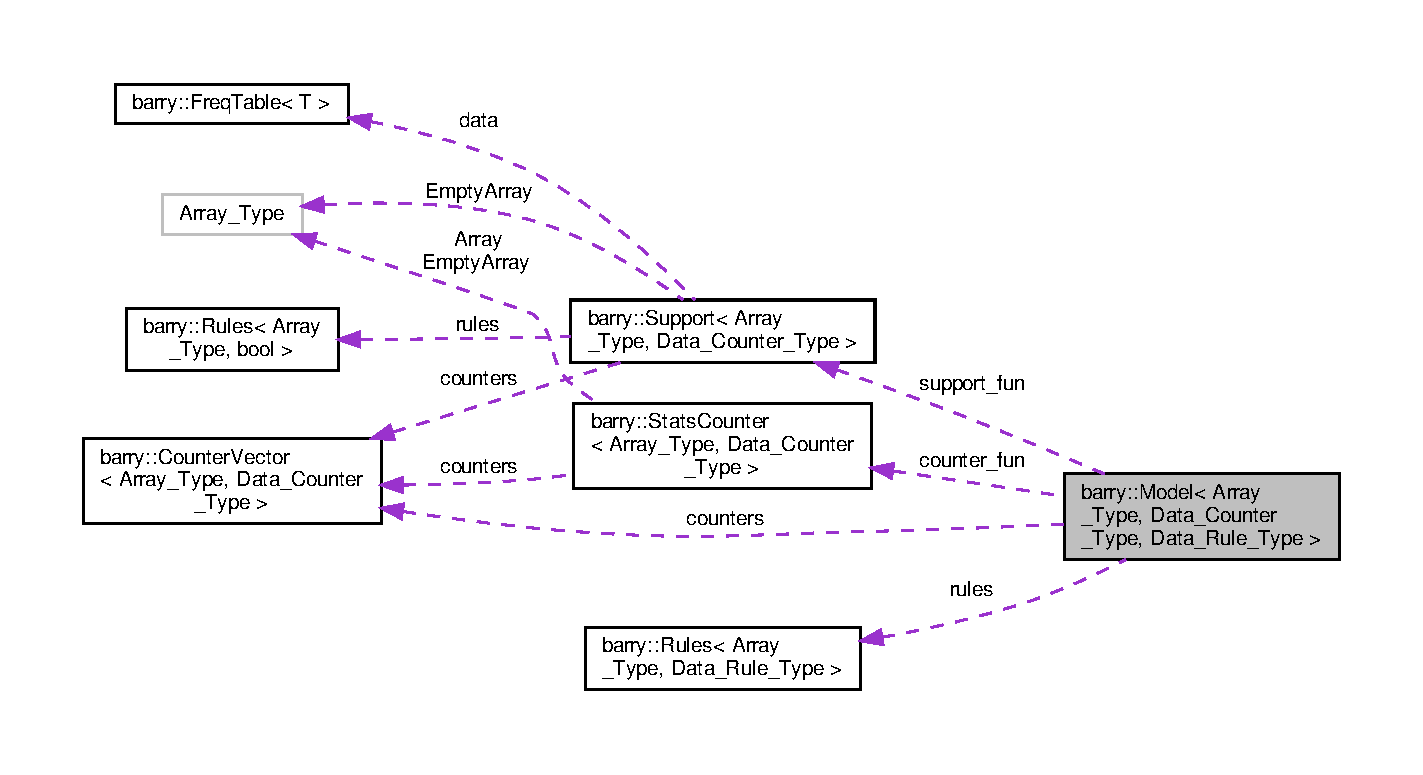
\includegraphics[width=350pt]{classbarry_1_1_model__coll__graph}
\end{center}
\end{figure}
\subsection*{Public Member Functions}
\begin{DoxyCompactItemize}
\item 
\hyperlink{classbarry_1_1_model_a29e6e0c37d9a892772c5ee95ce1e1043}{Model} ()
\item 
\hyperlink{classbarry_1_1_model_a46639bb435ca2992dac8858528a5362e}{Model} (\hyperlink{namespacebarry_a11dfc53ddb4672278319aa04f1e09a6c}{uint} size\+\_\+)
\item 
\hyperlink{classbarry_1_1_model_a047905a921baa9e51a4f07d337379375}{Model} (const \hyperlink{classbarry_1_1_model}{Model}$<$ Array\+\_\+\+Type, Data\+\_\+\+Counter\+\_\+\+Type, Data\+\_\+\+Rule\+\_\+\+Type $>$ \&Model\+\_\+)
\item 
\hyperlink{classbarry_1_1_model}{Model}$<$ Array\+\_\+\+Type, Data\+\_\+\+Counter\+\_\+\+Type, Data\+\_\+\+Rule\+\_\+\+Type $>$ \& \hyperlink{classbarry_1_1_model_a4944b5918dc4a9a59f72587da1e6bb3a}{operator=} (const \hyperlink{classbarry_1_1_model}{Model}$<$ Array\+\_\+\+Type, Data\+\_\+\+Counter\+\_\+\+Type, Data\+\_\+\+Rule\+\_\+\+Type $>$ \&Model\+\_\+)
\item 
\hyperlink{classbarry_1_1_model_a2b8617c8bb1b8c76bbaa0f596af0c132}{$\sim$\+Model} ()
\item 
void \hyperlink{classbarry_1_1_model_a06a6f52dfc6868908cf11e6663a93904}{store\+\_\+psets} ()
\item 
void \hyperlink{classbarry_1_1_model_add1847cdaf3f5bbde6c14efc2e4d16df}{set\+\_\+keygen} (std\+::function$<$ std\+::vector$<$ double $>$(const Array\+\_\+\+Type \&)$>$ keygen\+\_\+)
\item 
\hyperlink{namespacebarry_a11dfc53ddb4672278319aa04f1e09a6c}{uint} \hyperlink{classbarry_1_1_model_a17a2205b52c03bb29eefb8fb126a01f6}{add\+\_\+array} (const Array\+\_\+\+Type \&Array\+\_\+, bool force\+\_\+new=false)
\begin{DoxyCompactList}\small\item\em Adds an array to the support of not already included. \end{DoxyCompactList}\item 
void \hyperlink{classbarry_1_1_model_ac00b5c6a1446ad00fdf1d92c9cb1df3c}{print\+\_\+stats} (\hyperlink{namespacebarry_a11dfc53ddb4672278319aa04f1e09a6c}{uint} i) const
\item 
Array\+\_\+\+Type \hyperlink{classbarry_1_1_model_a1b7b9ad1362b8de49c00e7e8d5d3675e}{sample} (const Array\+\_\+\+Type \&Array\+\_\+, const std\+::vector$<$ double $>$ \&params=\{\})
\item 
Array\+\_\+\+Type \hyperlink{classbarry_1_1_model_a7fb66a67707f610b70ee05b814373f49}{sample} (const \hyperlink{namespacebarry_a11dfc53ddb4672278319aa04f1e09a6c}{uint} \&i, const std\+::vector$<$ double $>$ \&params)
\end{DoxyCompactItemize}
\begin{Indent}\textbf{ Wrappers for the `\+Counters` member.}\par
{\em These will add counters to the model, which are shared by the support and the actual counter function. }\begin{DoxyCompactItemize}
\item 
void \hyperlink{classbarry_1_1_model_a1548bd4681944c3eb761a22a38ef5547}{add\+\_\+counter} (\hyperlink{classbarry_1_1_counter}{Counter}$<$ Array\+\_\+\+Type, Data\+\_\+\+Counter\+\_\+\+Type $>$ \&counter)
\item 
void \hyperlink{classbarry_1_1_model_a6c1f524daf08e10888a49318030616c4}{add\+\_\+counter} (\hyperlink{classbarry_1_1_counter}{Counter}$<$ Array\+\_\+\+Type, Data\+\_\+\+Counter\+\_\+\+Type $>$ $\ast$counter)
\item 
void \hyperlink{classbarry_1_1_model_a4e4a18943bda513a844dc11aa088a698}{add\+\_\+counter} (\hyperlink{namespacebarry_abaaae3200da8e4b7faac3c04fe9c3081}{Counter\+\_\+fun\+\_\+type}$<$ Array\+\_\+\+Type, Data\+\_\+\+Counter\+\_\+\+Type $>$ count\+\_\+fun\+\_\+, \hyperlink{namespacebarry_abaaae3200da8e4b7faac3c04fe9c3081}{Counter\+\_\+fun\+\_\+type}$<$ Array\+\_\+\+Type, Data\+\_\+\+Counter\+\_\+\+Type $>$ init\+\_\+fun\+\_\+=nullptr, Data\+\_\+\+Counter\+\_\+\+Type $\ast$data\+\_\+=nullptr, bool delete\+\_\+data\+\_\+=false)
\item 
void \hyperlink{classbarry_1_1_model_aab2ba8c90b888cfa2143bccf42fcb89f}{set\+\_\+counters} (\hyperlink{classbarry_1_1_counters}{Counters}$<$ Array\+\_\+\+Type, Data\+\_\+\+Counter\+\_\+\+Type $>$ $\ast$counters\+\_\+)
\end{DoxyCompactItemize}
\end{Indent}
\begin{Indent}\textbf{ Wrappers for the `\+Rules` member.}\par
{\em These will add rules to the model, which are shared by the support and the actual counter function. }\begin{DoxyCompactItemize}
\item 
void \hyperlink{classbarry_1_1_model_af2c3f6300b90e6a2a4deaebaf2b0e732}{add\+\_\+rule} (\hyperlink{classbarry_1_1_rule}{Rule}$<$ Array\+\_\+\+Type, Data\+\_\+\+Rule\+\_\+\+Type $>$ \&rule)
\item 
void \hyperlink{classbarry_1_1_model_aba5b01457e2f624766a72ba15b8cb6be}{add\+\_\+rule} (\hyperlink{classbarry_1_1_rule}{Rule}$<$ Array\+\_\+\+Type, Data\+\_\+\+Rule\+\_\+\+Type $>$ $\ast$rule)
\item 
void \hyperlink{classbarry_1_1_model_af3a1a343dfff4f40443bee4ddf76a0ba}{add\+\_\+rule} (\hyperlink{namespacebarry_aefd7e6d4ba228e2ce1074d075c512178}{Rule\+\_\+fun\+\_\+type}$<$ Array\+\_\+\+Type, Data\+\_\+\+Rule\+\_\+\+Type $>$ count\+\_\+fun\+\_\+, Data\+\_\+\+Rule\+\_\+\+Type $\ast$data\+\_\+=nullptr, bool delete\+\_\+data\+\_\+=false)
\item 
void \hyperlink{classbarry_1_1_model_a86a46cf6fdc7c6514b97263f9ee4130b}{set\+\_\+rules} (\hyperlink{classbarry_1_1_rules}{Rules}$<$ Array\+\_\+\+Type, Data\+\_\+\+Rule\+\_\+\+Type $>$ $\ast$rules\+\_\+)
\end{DoxyCompactItemize}
\end{Indent}
\begin{Indent}\textbf{ Likelihood functions.}\par
{\em Calculation of likelihood functions is done reusing normalizing constants. Before recalculating the normalizing constant, the function checks whether {\ttfamily params} matches the last set vector of parameters used to compute it.


\begin{DoxyParams}{Parameters}
{\em params} & Vector of parameters \\
\hline
{\em as\+\_\+log} & When {\ttfamily true}, the function returns the log-\/likelihood. \\
\hline
\end{DoxyParams}
}\begin{DoxyCompactItemize}
\item 
double \hyperlink{classbarry_1_1_model_ae75fe2213980b6b245e279c7836ab99b}{likelihood} (const std\+::vector$<$ double $>$ \&params, const \hyperlink{namespacebarry_a11dfc53ddb4672278319aa04f1e09a6c}{uint} \&i, bool as\+\_\+log=false)
\item 
double \hyperlink{classbarry_1_1_model_a1a11a54860e22fbd152de4d7cfd30b89}{likelihood} (const std\+::vector$<$ double $>$ \&params, const Array\+\_\+\+Type \&Array\+\_\+, bool as\+\_\+log=false)
\item 
double \hyperlink{classbarry_1_1_model_ab88f541fc010f0ee1a415c9cb6c292b7}{likelihood} (const std\+::vector$<$ double $>$ \&params, const std\+::vector$<$ double $>$ \&target\+\_\+, const \hyperlink{namespacebarry_a11dfc53ddb4672278319aa04f1e09a6c}{uint} \&i, bool as\+\_\+log=false)
\item 
double \hyperlink{classbarry_1_1_model_a31d16ef478d772cedde0813575074a0f}{likelihood\+\_\+total} (const std\+::vector$<$ double $>$ \&params, bool as\+\_\+log=false)
\end{DoxyCompactItemize}
\end{Indent}
\begin{Indent}\textbf{ Extract elements by index}\par
{\em 
\begin{DoxyParams}{Parameters}
{\em i} & Index relative to the array in the model. \\
\hline
{\em params} & A new vector of model parameters to compute the normalizing constant. \\
\hline
{\em as\+\_\+log} & When {\ttfamily true} returns the logged version of the normalizing constant. \\
\hline
\end{DoxyParams}
}\begin{DoxyCompactItemize}
\item 
double \hyperlink{classbarry_1_1_model_a8de55fd86cdca46936e455721754a2af}{get\+\_\+norm\+\_\+const} (const std\+::vector$<$ double $>$ \&params, const \hyperlink{namespacebarry_a11dfc53ddb4672278319aa04f1e09a6c}{uint} \&i, bool as\+\_\+log=false)
\item 
const std\+::vector$<$ Array\+\_\+\+Type $>$ $\ast$ \hyperlink{classbarry_1_1_model_ad09221a8938765deec2c9d4d0fa8dec5}{get\+\_\+pset} (const \hyperlink{namespacebarry_a11dfc53ddb4672278319aa04f1e09a6c}{uint} \&i)
\item 
const std\+::vector$<$ std\+::vector$<$ double $>$ $>$ $\ast$ \hyperlink{classbarry_1_1_model_adde1cf74eb0ca7f771b7878af9766cdf}{get\+\_\+stats} (const \hyperlink{namespacebarry_a11dfc53ddb4672278319aa04f1e09a6c}{uint} \&i)
\end{DoxyCompactItemize}
\end{Indent}
\begin{Indent}\textbf{ Size of the model}\par
{\em Number of different supports included in the model

This will return the size of {\ttfamily stats}.

\begin{DoxyReturn}{Returns}
unsigned int 
\end{DoxyReturn}
}\begin{DoxyCompactItemize}
\item 
unsigned int \hyperlink{classbarry_1_1_model_ab3f157dbb542a48fe5bf412ff7d467fd}{size} () const
\item 
unsigned int \hyperlink{classbarry_1_1_model_a4b5edbe891b6da2319ea3fa6f1aba11d}{size\+\_\+unique} () const
\end{DoxyCompactItemize}
\end{Indent}
\subsection*{Public Attributes}
\begin{DoxyCompactItemize}
\item 
std\+::vector$<$ \hyperlink{namespacebarry_a3e2d8c3b6cf602107559d4237d9f1315}{Counts\+\_\+type} $>$ \hyperlink{classbarry_1_1_model_a09fa1641ee40f23bad698a7c78db4b87}{stats}
\item 
std\+::vector$<$ \hyperlink{namespacebarry_a11dfc53ddb4672278319aa04f1e09a6c}{uint} $>$ \hyperlink{classbarry_1_1_model_a6e72cbb235cf592668c286931a488830}{n\+\_\+arrays\+\_\+per\+\_\+stats}
\item 
\hyperlink{namespacebarry_a2f0d3aab1d67e4c8eaeab9022e16139f}{Map\+Vec\+\_\+type}$<$ double, \hyperlink{namespacebarry_a11dfc53ddb4672278319aa04f1e09a6c}{uint} $>$ \hyperlink{classbarry_1_1_model_a802069270d02f2e2ad7e5f2adb51c2bc}{keys2support}
\begin{DoxyCompactList}\small\item\em Map of types of arrays to support sets. \end{DoxyCompactList}\item 
std\+::vector$<$ std\+::vector$<$ double $>$ $>$ \hyperlink{classbarry_1_1_model_ace8577c5c0c7bd927a2337515155ab6f}{params\+\_\+last}
\begin{DoxyCompactList}\small\item\em Vector of the previously used parameters. \end{DoxyCompactList}\item 
std\+::vector$<$ double $>$ \hyperlink{classbarry_1_1_model_a600630f5fad408c157b21404dbde4bc1}{normalizing\+\_\+constants}
\item 
std\+::vector$<$ bool $>$ \hyperlink{classbarry_1_1_model_ae7b6def02fcb353830362713490c9825}{first\+\_\+calc\+\_\+done}
\item 
std\+::function$<$ std\+::vector$<$ double $>$const Array\+\_\+\+Type \&)$>$ \hyperlink{classbarry_1_1_model_a68f7422006423a4f0a00c3e4f5d0e1d5}{keygen} = nullptr
\begin{DoxyCompactList}\small\item\em Function to extract features of the array to be hash. \end{DoxyCompactList}\end{DoxyCompactItemize}
\begin{Indent}\textbf{ Container space for the powerset (and its sufficient stats)}\par
{\em This is useful in the case of using simulations or evaluating functions that need to account for the full set of states. }\begin{DoxyCompactItemize}
\item 
bool \hyperlink{classbarry_1_1_model_a08c74ccd0aa76906f724ccb5e36d0762}{with\+\_\+pset} = false
\item 
std\+::vector$<$ std\+::vector$<$ Array\+\_\+\+Type $>$ $>$ \hyperlink{classbarry_1_1_model_ae5aad2049cc19ee36e9c2cfefd65a0dd}{pset\+\_\+arrays}
\item 
std\+::vector$<$ std\+::vector$<$ std\+::vector$<$ double $>$ $>$ $>$ \hyperlink{classbarry_1_1_model_a3763f129965942611eb58e9779336f34}{pset\+\_\+stats}
\item 
std\+::vector$<$ std\+::vector$<$ double $>$ $>$ \hyperlink{classbarry_1_1_model_a4ccabb6842238fa5c7ff3476ef760423}{pset\+\_\+probs}
\end{DoxyCompactItemize}
\end{Indent}
\begin{Indent}\textbf{ Information about the arrays used in the model}\par
{\em {\ttfamily target\+\_\+stats} holds the observed sufficient statistics for each array in the dataset. {\ttfamily array\+\_\+frequency} contains the frequency with which each of the target stats (arrays) shows in the support. {\ttfamily array2support} maps array indices (0, 1, ...) to the corresponding support. }\begin{DoxyCompactItemize}
\item 
std\+::vector$<$ std\+::vector$<$ double $>$ $>$ \hyperlink{classbarry_1_1_model_ab2a0fde37b6a6da5a5faffcd24ec4c27}{target\+\_\+stats}
\item 
std\+::vector$<$ \hyperlink{namespacebarry_a11dfc53ddb4672278319aa04f1e09a6c}{uint} $>$ \hyperlink{classbarry_1_1_model_a64041df6ecac9aface20f9d13c0b22eb}{array\+\_\+frequency}
\item 
std\+::vector$<$ \hyperlink{namespacebarry_a11dfc53ddb4672278319aa04f1e09a6c}{uint} $>$ \hyperlink{classbarry_1_1_model_a9cd0e9c9d29df6637ab30ebe3daeeff7}{arrays2support}
\end{DoxyCompactItemize}
\end{Indent}
\begin{Indent}\textbf{ Functions to compute statistics}\par
{\em Arguments are recycled to save memory and computation. }\begin{DoxyCompactItemize}
\item 
\hyperlink{classbarry_1_1_counters}{Counters}$<$ Array\+\_\+\+Type, Data\+\_\+\+Counter\+\_\+\+Type $>$ \hyperlink{classbarry_1_1_model_aea013a7ac325ece7564e8ea9cdf441a2}{counters}
\item 
\hyperlink{classbarry_1_1_rules}{Rules}$<$ Array\+\_\+\+Type, Data\+\_\+\+Rule\+\_\+\+Type $>$ \hyperlink{classbarry_1_1_model_a53e5242ce0ed2bc7194a0662d09493f2}{rules}
\item 
\hyperlink{classbarry_1_1_support}{Support}$<$ Array\+\_\+\+Type, Data\+\_\+\+Counter\+\_\+\+Type, Data\+\_\+\+Rule\+\_\+\+Type $>$ \hyperlink{classbarry_1_1_model_afd005aae0fdd12a8c68d1fd8823b3727}{support\+\_\+fun}
\item 
\hyperlink{classbarry_1_1_stats_counter}{Stats\+Counter}$<$ Array\+\_\+\+Type, Data\+\_\+\+Counter\+\_\+\+Type $>$ \hyperlink{classbarry_1_1_model_ada40ca4ec8b21a3dbbe646edbfb1df45}{counter\+\_\+fun}
\end{DoxyCompactItemize}
\end{Indent}
\subsection*{Random number generation}
\label{_amgrp9e5d9cca94c03e04e66d088f8628d19b}%
Random number generation \begin{DoxyCompactItemize}
\item 
std\+::mt19937 $\ast$ \hyperlink{classbarry_1_1_model_adc85f6765d272293333a83bc2a4e90d2}{rengine} = nullptr
\item 
bool \hyperlink{classbarry_1_1_model_afe239e83969b6b99eddf1ecd509bc8f2}{rengine\+\_\+deleted} = true
\item 
void \hyperlink{classbarry_1_1_model_a1e1cdb67d12968394dbd68dad0cff208}{set\+\_\+rengine} (std\+::mt19937 $\ast$rengine\+\_\+, bool delete\+\_\+=false)
\item 
void \hyperlink{classbarry_1_1_model_a175a1772d843dedd603f6bb572cfa30a}{set\+\_\+seed} (unsigned int s)
\end{DoxyCompactItemize}


\subsection{Detailed Description}
\subsubsection*{template$<$typename Array\+\_\+\+Type = B\+Array$<$$>$, typename Data\+\_\+\+Counter\+\_\+\+Type = bool, typename Data\+\_\+\+Rule\+\_\+\+Type = bool$>$\newline
class barry\+::\+Model$<$ Array\+\_\+\+Type, Data\+\_\+\+Counter\+\_\+\+Type, Data\+\_\+\+Rule\+\_\+\+Type $>$}

General framework for discrete exponential models. This class allows generating discrete exponential models in the form of a linear exponential model\+: \[ \frac{ \exp{\left(\theta^{\mbox{t}}c(A)\right)} }{ \sum_{A'\in \mathcal{A}}\exp{\left(\theta^{\mbox{t}}c(A')\right)} } \]. 

This implementation aims to reduce the number of times that the support needs to be computed. Models included here use more than a single array, and thus allow the function to recycle support sets as needed. For example, if we are looking at directed graphs all of the same size and without vertex level features, i.\+e. a model that only counts edges, triangles, etc. then the support needs to be fully computed only once.


\begin{DoxyTemplParams}{Template Parameters}
{\em Array\+\_\+\+Type} & Class of {\ttfamily \hyperlink{classbarry_1_1_b_array}{B\+Array}} object. \\
\hline
{\em Data\+\_\+\+Counter\+\_\+\+Type} & Any type. \\
\hline
{\em Data\+\_\+\+Rule\+\_\+\+Type} & Any type. \\
\hline
\end{DoxyTemplParams}


Definition at line 95 of file barry.\+hpp.



\subsection{Constructor \& Destructor Documentation}
\mbox{\Hypertarget{classbarry_1_1_model_a29e6e0c37d9a892772c5ee95ce1e1043}\label{classbarry_1_1_model_a29e6e0c37d9a892772c5ee95ce1e1043}} 
\index{barry\+::\+Model@{barry\+::\+Model}!Model@{Model}}
\index{Model@{Model}!barry\+::\+Model@{barry\+::\+Model}}
\subsubsection{\texorpdfstring{Model()}{Model()}\hspace{0.1cm}{\footnotesize\ttfamily [1/3]}}
{\footnotesize\ttfamily template$<$typename Array\+\_\+\+Type , typename Data\+\_\+\+Counter\+\_\+\+Type , typename Data\+\_\+\+Rule\+\_\+\+Type $>$ \\
\hyperlink{classbarry_1_1_model}{Model}$<$ Array\+\_\+\+Type, Data\+\_\+\+Counter\+\_\+\+Type, Data\+\_\+\+Rule\+\_\+\+Type $>$\+::\hyperlink{classbarry_1_1_model}{Model} (\begin{DoxyParamCaption}{ }\end{DoxyParamCaption})\hspace{0.3cm}{\ttfamily [inline]}}



Definition at line 7 of file barry.\+hpp.

\mbox{\Hypertarget{classbarry_1_1_model_a46639bb435ca2992dac8858528a5362e}\label{classbarry_1_1_model_a46639bb435ca2992dac8858528a5362e}} 
\index{barry\+::\+Model@{barry\+::\+Model}!Model@{Model}}
\index{Model@{Model}!barry\+::\+Model@{barry\+::\+Model}}
\subsubsection{\texorpdfstring{Model()}{Model()}\hspace{0.1cm}{\footnotesize\ttfamily [2/3]}}
{\footnotesize\ttfamily template$<$typename Array\+\_\+\+Type , typename Data\+\_\+\+Counter\+\_\+\+Type , typename Data\+\_\+\+Rule\+\_\+\+Type $>$ \\
\hyperlink{classbarry_1_1_model}{Model}$<$ Array\+\_\+\+Type, Data\+\_\+\+Counter\+\_\+\+Type, Data\+\_\+\+Rule\+\_\+\+Type $>$\+::\hyperlink{classbarry_1_1_model}{Model} (\begin{DoxyParamCaption}\item[{\hyperlink{namespacebarry_a11dfc53ddb4672278319aa04f1e09a6c}{uint}}]{size\+\_\+ }\end{DoxyParamCaption})\hspace{0.3cm}{\ttfamily [inline]}}



Definition at line 27 of file barry.\+hpp.

\mbox{\Hypertarget{classbarry_1_1_model_a047905a921baa9e51a4f07d337379375}\label{classbarry_1_1_model_a047905a921baa9e51a4f07d337379375}} 
\index{barry\+::\+Model@{barry\+::\+Model}!Model@{Model}}
\index{Model@{Model}!barry\+::\+Model@{barry\+::\+Model}}
\subsubsection{\texorpdfstring{Model()}{Model()}\hspace{0.1cm}{\footnotesize\ttfamily [3/3]}}
{\footnotesize\ttfamily template$<$typename Array\+\_\+\+Type , typename Data\+\_\+\+Counter\+\_\+\+Type , typename Data\+\_\+\+Rule\+\_\+\+Type $>$ \\
\hyperlink{classbarry_1_1_model}{Model}$<$ Array\+\_\+\+Type, Data\+\_\+\+Counter\+\_\+\+Type, Data\+\_\+\+Rule\+\_\+\+Type $>$\+::\hyperlink{classbarry_1_1_model}{Model} (\begin{DoxyParamCaption}\item[{const \hyperlink{classbarry_1_1_model}{Model}$<$ Array\+\_\+\+Type, Data\+\_\+\+Counter\+\_\+\+Type, Data\+\_\+\+Rule\+\_\+\+Type $>$ \&}]{Model\+\_\+ }\end{DoxyParamCaption})\hspace{0.3cm}{\ttfamily [inline]}}



Definition at line 50 of file barry.\+hpp.

\mbox{\Hypertarget{classbarry_1_1_model_a2b8617c8bb1b8c76bbaa0f596af0c132}\label{classbarry_1_1_model_a2b8617c8bb1b8c76bbaa0f596af0c132}} 
\index{barry\+::\+Model@{barry\+::\+Model}!````~Model@{$\sim$\+Model}}
\index{````~Model@{$\sim$\+Model}!barry\+::\+Model@{barry\+::\+Model}}
\subsubsection{\texorpdfstring{$\sim$\+Model()}{~Model()}}
{\footnotesize\ttfamily template$<$typename Array\+\_\+\+Type  = B\+Array$<$$>$, typename Data\+\_\+\+Counter\+\_\+\+Type  = bool, typename Data\+\_\+\+Rule\+\_\+\+Type  = bool$>$ \\
\hyperlink{classbarry_1_1_model}{barry\+::\+Model}$<$ Array\+\_\+\+Type, Data\+\_\+\+Counter\+\_\+\+Type, Data\+\_\+\+Rule\+\_\+\+Type $>$\+::$\sim$\hyperlink{classbarry_1_1_model}{Model} (\begin{DoxyParamCaption}{ }\end{DoxyParamCaption})\hspace{0.3cm}{\ttfamily [inline]}}



Definition at line 186 of file barry.\+hpp.



\subsection{Member Function Documentation}
\mbox{\Hypertarget{classbarry_1_1_model_a17a2205b52c03bb29eefb8fb126a01f6}\label{classbarry_1_1_model_a17a2205b52c03bb29eefb8fb126a01f6}} 
\index{barry\+::\+Model@{barry\+::\+Model}!add\+\_\+array@{add\+\_\+array}}
\index{add\+\_\+array@{add\+\_\+array}!barry\+::\+Model@{barry\+::\+Model}}
\subsubsection{\texorpdfstring{add\+\_\+array()}{add\_array()}}
{\footnotesize\ttfamily template$<$typename Array\+\_\+\+Type , typename Data\+\_\+\+Counter\+\_\+\+Type , typename Data\+\_\+\+Rule\+\_\+\+Type $>$ \\
\hyperlink{namespacebarry_a11dfc53ddb4672278319aa04f1e09a6c}{uint} \hyperlink{classbarry_1_1_model}{Model}$<$ Array\+\_\+\+Type, Data\+\_\+\+Counter\+\_\+\+Type, Data\+\_\+\+Rule\+\_\+\+Type $>$\+::add\+\_\+array (\begin{DoxyParamCaption}\item[{const Array\+\_\+\+Type \&}]{Array\+\_\+,  }\item[{bool}]{force\+\_\+new = {\ttfamily false} }\end{DoxyParamCaption})\hspace{0.3cm}{\ttfamily [inline]}}



Adds an array to the support of not already included. 


\begin{DoxyParams}{Parameters}
{\em Array\+\_\+} & array to be added \\
\hline
{\em force\+\_\+new} & If {\ttfamily false}, it will use {\ttfamily keygen} to obtain a double vector and create a hash of it. If the hash has been computed earlier, the support is recycled.\\
\hline
\end{DoxyParams}
\begin{DoxyReturn}{Returns}
The number of the array. 
\end{DoxyReturn}
When computing with the powerset, we need to grow the corresponding vectors on the fly 

Definition at line 229 of file barry.\+hpp.

\mbox{\Hypertarget{classbarry_1_1_model_a1548bd4681944c3eb761a22a38ef5547}\label{classbarry_1_1_model_a1548bd4681944c3eb761a22a38ef5547}} 
\index{barry\+::\+Model@{barry\+::\+Model}!add\+\_\+counter@{add\+\_\+counter}}
\index{add\+\_\+counter@{add\+\_\+counter}!barry\+::\+Model@{barry\+::\+Model}}
\subsubsection{\texorpdfstring{add\+\_\+counter()}{add\_counter()}\hspace{0.1cm}{\footnotesize\ttfamily [1/3]}}
{\footnotesize\ttfamily template$<$typename Array\+\_\+\+Type , typename Data\+\_\+\+Counter\+\_\+\+Type , typename Data\+\_\+\+Rule\+\_\+\+Type $>$ \\
void \hyperlink{classbarry_1_1_model}{Model}$<$ Array\+\_\+\+Type, Data\+\_\+\+Counter\+\_\+\+Type, Data\+\_\+\+Rule\+\_\+\+Type $>$\+::add\+\_\+counter (\begin{DoxyParamCaption}\item[{\hyperlink{classbarry_1_1_counter}{Counter}$<$ Array\+\_\+\+Type, Data\+\_\+\+Counter\+\_\+\+Type $>$ \&}]{counter }\end{DoxyParamCaption})\hspace{0.3cm}{\ttfamily [inline]}}



Definition at line 131 of file barry.\+hpp.

\mbox{\Hypertarget{classbarry_1_1_model_a6c1f524daf08e10888a49318030616c4}\label{classbarry_1_1_model_a6c1f524daf08e10888a49318030616c4}} 
\index{barry\+::\+Model@{barry\+::\+Model}!add\+\_\+counter@{add\+\_\+counter}}
\index{add\+\_\+counter@{add\+\_\+counter}!barry\+::\+Model@{barry\+::\+Model}}
\subsubsection{\texorpdfstring{add\+\_\+counter()}{add\_counter()}\hspace{0.1cm}{\footnotesize\ttfamily [2/3]}}
{\footnotesize\ttfamily template$<$typename Array\+\_\+\+Type , typename Data\+\_\+\+Counter\+\_\+\+Type , typename Data\+\_\+\+Rule\+\_\+\+Type $>$ \\
void \hyperlink{classbarry_1_1_model}{Model}$<$ Array\+\_\+\+Type, Data\+\_\+\+Counter\+\_\+\+Type, Data\+\_\+\+Rule\+\_\+\+Type $>$\+::add\+\_\+counter (\begin{DoxyParamCaption}\item[{\hyperlink{classbarry_1_1_counter}{Counter}$<$ Array\+\_\+\+Type, Data\+\_\+\+Counter\+\_\+\+Type $>$ $\ast$}]{counter }\end{DoxyParamCaption})\hspace{0.3cm}{\ttfamily [inline]}}



Definition at line 140 of file barry.\+hpp.

\mbox{\Hypertarget{classbarry_1_1_model_a4e4a18943bda513a844dc11aa088a698}\label{classbarry_1_1_model_a4e4a18943bda513a844dc11aa088a698}} 
\index{barry\+::\+Model@{barry\+::\+Model}!add\+\_\+counter@{add\+\_\+counter}}
\index{add\+\_\+counter@{add\+\_\+counter}!barry\+::\+Model@{barry\+::\+Model}}
\subsubsection{\texorpdfstring{add\+\_\+counter()}{add\_counter()}\hspace{0.1cm}{\footnotesize\ttfamily [3/3]}}
{\footnotesize\ttfamily template$<$typename Array\+\_\+\+Type , typename Data\+\_\+\+Counter\+\_\+\+Type , typename Data\+\_\+\+Rule\+\_\+\+Type $>$ \\
void \hyperlink{classbarry_1_1_model}{Model}$<$ Array\+\_\+\+Type, Data\+\_\+\+Counter\+\_\+\+Type, Data\+\_\+\+Rule\+\_\+\+Type $>$\+::add\+\_\+counter (\begin{DoxyParamCaption}\item[{\hyperlink{namespacebarry_abaaae3200da8e4b7faac3c04fe9c3081}{Counter\+\_\+fun\+\_\+type}$<$ Array\+\_\+\+Type, Data\+\_\+\+Counter\+\_\+\+Type $>$}]{count\+\_\+fun\+\_\+,  }\item[{\hyperlink{namespacebarry_abaaae3200da8e4b7faac3c04fe9c3081}{Counter\+\_\+fun\+\_\+type}$<$ Array\+\_\+\+Type, Data\+\_\+\+Counter\+\_\+\+Type $>$}]{init\+\_\+fun\+\_\+ = {\ttfamily nullptr},  }\item[{Data\+\_\+\+Counter\+\_\+\+Type $\ast$}]{data\+\_\+ = {\ttfamily nullptr},  }\item[{bool}]{delete\+\_\+data\+\_\+ = {\ttfamily false} }\end{DoxyParamCaption})\hspace{0.3cm}{\ttfamily [inline]}}



Definition at line 150 of file barry.\+hpp.

\mbox{\Hypertarget{classbarry_1_1_model_af2c3f6300b90e6a2a4deaebaf2b0e732}\label{classbarry_1_1_model_af2c3f6300b90e6a2a4deaebaf2b0e732}} 
\index{barry\+::\+Model@{barry\+::\+Model}!add\+\_\+rule@{add\+\_\+rule}}
\index{add\+\_\+rule@{add\+\_\+rule}!barry\+::\+Model@{barry\+::\+Model}}
\subsubsection{\texorpdfstring{add\+\_\+rule()}{add\_rule()}\hspace{0.1cm}{\footnotesize\ttfamily [1/3]}}
{\footnotesize\ttfamily template$<$typename Array\+\_\+\+Type , typename Data\+\_\+\+Counter\+\_\+\+Type , typename Data\+\_\+\+Rule\+\_\+\+Type $>$ \\
void \hyperlink{classbarry_1_1_model}{Model}$<$ Array\+\_\+\+Type, Data\+\_\+\+Counter\+\_\+\+Type, Data\+\_\+\+Rule\+\_\+\+Type $>$\+::add\+\_\+rule (\begin{DoxyParamCaption}\item[{\hyperlink{classbarry_1_1_rule}{Rule}$<$ Array\+\_\+\+Type, Data\+\_\+\+Rule\+\_\+\+Type $>$ \&}]{rule }\end{DoxyParamCaption})\hspace{0.3cm}{\ttfamily [inline]}}



Definition at line 182 of file barry.\+hpp.

\mbox{\Hypertarget{classbarry_1_1_model_aba5b01457e2f624766a72ba15b8cb6be}\label{classbarry_1_1_model_aba5b01457e2f624766a72ba15b8cb6be}} 
\index{barry\+::\+Model@{barry\+::\+Model}!add\+\_\+rule@{add\+\_\+rule}}
\index{add\+\_\+rule@{add\+\_\+rule}!barry\+::\+Model@{barry\+::\+Model}}
\subsubsection{\texorpdfstring{add\+\_\+rule()}{add\_rule()}\hspace{0.1cm}{\footnotesize\ttfamily [2/3]}}
{\footnotesize\ttfamily template$<$typename Array\+\_\+\+Type , typename Data\+\_\+\+Counter\+\_\+\+Type , typename Data\+\_\+\+Rule\+\_\+\+Type $>$ \\
void \hyperlink{classbarry_1_1_model}{Model}$<$ Array\+\_\+\+Type, Data\+\_\+\+Counter\+\_\+\+Type, Data\+\_\+\+Rule\+\_\+\+Type $>$\+::add\+\_\+rule (\begin{DoxyParamCaption}\item[{\hyperlink{classbarry_1_1_rule}{Rule}$<$ Array\+\_\+\+Type, Data\+\_\+\+Rule\+\_\+\+Type $>$ $\ast$}]{rule }\end{DoxyParamCaption})\hspace{0.3cm}{\ttfamily [inline]}}



Definition at line 191 of file barry.\+hpp.

\mbox{\Hypertarget{classbarry_1_1_model_af3a1a343dfff4f40443bee4ddf76a0ba}\label{classbarry_1_1_model_af3a1a343dfff4f40443bee4ddf76a0ba}} 
\index{barry\+::\+Model@{barry\+::\+Model}!add\+\_\+rule@{add\+\_\+rule}}
\index{add\+\_\+rule@{add\+\_\+rule}!barry\+::\+Model@{barry\+::\+Model}}
\subsubsection{\texorpdfstring{add\+\_\+rule()}{add\_rule()}\hspace{0.1cm}{\footnotesize\ttfamily [3/3]}}
{\footnotesize\ttfamily template$<$typename Array\+\_\+\+Type , typename Data\+\_\+\+Counter\+\_\+\+Type , typename Data\+\_\+\+Rule\+\_\+\+Type $>$ \\
void \hyperlink{classbarry_1_1_model}{Model}$<$ Array\+\_\+\+Type, Data\+\_\+\+Counter\+\_\+\+Type, Data\+\_\+\+Rule\+\_\+\+Type $>$\+::add\+\_\+rule (\begin{DoxyParamCaption}\item[{\hyperlink{namespacebarry_aefd7e6d4ba228e2ce1074d075c512178}{Rule\+\_\+fun\+\_\+type}$<$ Array\+\_\+\+Type, Data\+\_\+\+Rule\+\_\+\+Type $>$}]{count\+\_\+fun\+\_\+,  }\item[{Data\+\_\+\+Rule\+\_\+\+Type $\ast$}]{data\+\_\+ = {\ttfamily nullptr},  }\item[{bool}]{delete\+\_\+data\+\_\+ = {\ttfamily false} }\end{DoxyParamCaption})\hspace{0.3cm}{\ttfamily [inline]}}



Definition at line 201 of file barry.\+hpp.

\mbox{\Hypertarget{classbarry_1_1_model_a8de55fd86cdca46936e455721754a2af}\label{classbarry_1_1_model_a8de55fd86cdca46936e455721754a2af}} 
\index{barry\+::\+Model@{barry\+::\+Model}!get\+\_\+norm\+\_\+const@{get\+\_\+norm\+\_\+const}}
\index{get\+\_\+norm\+\_\+const@{get\+\_\+norm\+\_\+const}!barry\+::\+Model@{barry\+::\+Model}}
\subsubsection{\texorpdfstring{get\+\_\+norm\+\_\+const()}{get\_norm\_const()}}
{\footnotesize\ttfamily template$<$typename Array\+\_\+\+Type , typename Data\+\_\+\+Counter\+\_\+\+Type , typename Data\+\_\+\+Rule\+\_\+\+Type $>$ \\
double \hyperlink{classbarry_1_1_model}{Model}$<$ Array\+\_\+\+Type, Data\+\_\+\+Counter\+\_\+\+Type, Data\+\_\+\+Rule\+\_\+\+Type $>$\+::get\+\_\+norm\+\_\+const (\begin{DoxyParamCaption}\item[{const std\+::vector$<$ double $>$ \&}]{params,  }\item[{const \hyperlink{namespacebarry_a11dfc53ddb4672278319aa04f1e09a6c}{uint} \&}]{i,  }\item[{bool}]{as\+\_\+log = {\ttfamily false} }\end{DoxyParamCaption})\hspace{0.3cm}{\ttfamily [inline]}}



Definition at line 440 of file barry.\+hpp.

\mbox{\Hypertarget{classbarry_1_1_model_ad09221a8938765deec2c9d4d0fa8dec5}\label{classbarry_1_1_model_ad09221a8938765deec2c9d4d0fa8dec5}} 
\index{barry\+::\+Model@{barry\+::\+Model}!get\+\_\+pset@{get\+\_\+pset}}
\index{get\+\_\+pset@{get\+\_\+pset}!barry\+::\+Model@{barry\+::\+Model}}
\subsubsection{\texorpdfstring{get\+\_\+pset()}{get\_pset()}}
{\footnotesize\ttfamily template$<$typename Array\+\_\+\+Type , typename Data\+\_\+\+Counter\+\_\+\+Type , typename Data\+\_\+\+Rule\+\_\+\+Type $>$ \\
const std\+::vector$<$ Array\+\_\+\+Type $>$ $\ast$ \hyperlink{classbarry_1_1_model}{Model}$<$ Array\+\_\+\+Type, Data\+\_\+\+Counter\+\_\+\+Type, Data\+\_\+\+Rule\+\_\+\+Type $>$\+::get\+\_\+pset (\begin{DoxyParamCaption}\item[{const \hyperlink{namespacebarry_a11dfc53ddb4672278319aa04f1e09a6c}{uint} \&}]{i }\end{DoxyParamCaption})\hspace{0.3cm}{\ttfamily [inline]}}



Definition at line 472 of file barry.\+hpp.

\mbox{\Hypertarget{classbarry_1_1_model_adde1cf74eb0ca7f771b7878af9766cdf}\label{classbarry_1_1_model_adde1cf74eb0ca7f771b7878af9766cdf}} 
\index{barry\+::\+Model@{barry\+::\+Model}!get\+\_\+stats@{get\+\_\+stats}}
\index{get\+\_\+stats@{get\+\_\+stats}!barry\+::\+Model@{barry\+::\+Model}}
\subsubsection{\texorpdfstring{get\+\_\+stats()}{get\_stats()}}
{\footnotesize\ttfamily template$<$typename Array\+\_\+\+Type , typename Data\+\_\+\+Counter\+\_\+\+Type , typename Data\+\_\+\+Rule\+\_\+\+Type $>$ \\
const std\+::vector$<$ std\+::vector$<$ double $>$ $>$ $\ast$ \hyperlink{classbarry_1_1_model}{Model}$<$ Array\+\_\+\+Type, Data\+\_\+\+Counter\+\_\+\+Type, Data\+\_\+\+Rule\+\_\+\+Type $>$\+::get\+\_\+stats (\begin{DoxyParamCaption}\item[{const \hyperlink{namespacebarry_a11dfc53ddb4672278319aa04f1e09a6c}{uint} \&}]{i }\end{DoxyParamCaption})\hspace{0.3cm}{\ttfamily [inline]}}



Definition at line 485 of file barry.\+hpp.

\mbox{\Hypertarget{classbarry_1_1_model_ae75fe2213980b6b245e279c7836ab99b}\label{classbarry_1_1_model_ae75fe2213980b6b245e279c7836ab99b}} 
\index{barry\+::\+Model@{barry\+::\+Model}!likelihood@{likelihood}}
\index{likelihood@{likelihood}!barry\+::\+Model@{barry\+::\+Model}}
\subsubsection{\texorpdfstring{likelihood()}{likelihood()}\hspace{0.1cm}{\footnotesize\ttfamily [1/3]}}
{\footnotesize\ttfamily template$<$typename Array\+\_\+\+Type , typename Data\+\_\+\+Counter\+\_\+\+Type , typename Data\+\_\+\+Rule\+\_\+\+Type $>$ \\
double \hyperlink{classbarry_1_1_model}{Model}$<$ Array\+\_\+\+Type, Data\+\_\+\+Counter\+\_\+\+Type, Data\+\_\+\+Rule\+\_\+\+Type $>$\+::likelihood (\begin{DoxyParamCaption}\item[{const std\+::vector$<$ double $>$ \&}]{params,  }\item[{const \hyperlink{namespacebarry_a11dfc53ddb4672278319aa04f1e09a6c}{uint} \&}]{i,  }\item[{bool}]{as\+\_\+log = {\ttfamily false} }\end{DoxyParamCaption})\hspace{0.3cm}{\ttfamily [inline]}}



Definition at line 313 of file barry.\+hpp.

\mbox{\Hypertarget{classbarry_1_1_model_a1a11a54860e22fbd152de4d7cfd30b89}\label{classbarry_1_1_model_a1a11a54860e22fbd152de4d7cfd30b89}} 
\index{barry\+::\+Model@{barry\+::\+Model}!likelihood@{likelihood}}
\index{likelihood@{likelihood}!barry\+::\+Model@{barry\+::\+Model}}
\subsubsection{\texorpdfstring{likelihood()}{likelihood()}\hspace{0.1cm}{\footnotesize\ttfamily [2/3]}}
{\footnotesize\ttfamily template$<$typename Array\+\_\+\+Type , typename Data\+\_\+\+Counter\+\_\+\+Type , typename Data\+\_\+\+Rule\+\_\+\+Type $>$ \\
double \hyperlink{classbarry_1_1_model}{Model}$<$ Array\+\_\+\+Type, Data\+\_\+\+Counter\+\_\+\+Type, Data\+\_\+\+Rule\+\_\+\+Type $>$\+::likelihood (\begin{DoxyParamCaption}\item[{const std\+::vector$<$ double $>$ \&}]{params,  }\item[{const Array\+\_\+\+Type \&}]{Array\+\_\+,  }\item[{bool}]{as\+\_\+log = {\ttfamily false} }\end{DoxyParamCaption})\hspace{0.3cm}{\ttfamily [inline]}}



Definition at line 346 of file barry.\+hpp.

\mbox{\Hypertarget{classbarry_1_1_model_ab88f541fc010f0ee1a415c9cb6c292b7}\label{classbarry_1_1_model_ab88f541fc010f0ee1a415c9cb6c292b7}} 
\index{barry\+::\+Model@{barry\+::\+Model}!likelihood@{likelihood}}
\index{likelihood@{likelihood}!barry\+::\+Model@{barry\+::\+Model}}
\subsubsection{\texorpdfstring{likelihood()}{likelihood()}\hspace{0.1cm}{\footnotesize\ttfamily [3/3]}}
{\footnotesize\ttfamily template$<$typename Array\+\_\+\+Type , typename Data\+\_\+\+Counter\+\_\+\+Type , typename Data\+\_\+\+Rule\+\_\+\+Type $>$ \\
double \hyperlink{classbarry_1_1_model}{Model}$<$ Array\+\_\+\+Type, Data\+\_\+\+Counter\+\_\+\+Type, Data\+\_\+\+Rule\+\_\+\+Type $>$\+::likelihood (\begin{DoxyParamCaption}\item[{const std\+::vector$<$ double $>$ \&}]{params,  }\item[{const std\+::vector$<$ double $>$ \&}]{target\+\_\+,  }\item[{const \hyperlink{namespacebarry_a11dfc53ddb4672278319aa04f1e09a6c}{uint} \&}]{i,  }\item[{bool}]{as\+\_\+log = {\ttfamily false} }\end{DoxyParamCaption})\hspace{0.3cm}{\ttfamily [inline]}}



Definition at line 366 of file barry.\+hpp.

\mbox{\Hypertarget{classbarry_1_1_model_a31d16ef478d772cedde0813575074a0f}\label{classbarry_1_1_model_a31d16ef478d772cedde0813575074a0f}} 
\index{barry\+::\+Model@{barry\+::\+Model}!likelihood\+\_\+total@{likelihood\+\_\+total}}
\index{likelihood\+\_\+total@{likelihood\+\_\+total}!barry\+::\+Model@{barry\+::\+Model}}
\subsubsection{\texorpdfstring{likelihood\+\_\+total()}{likelihood\_total()}}
{\footnotesize\ttfamily template$<$typename Array\+\_\+\+Type , typename Data\+\_\+\+Counter\+\_\+\+Type , typename Data\+\_\+\+Rule\+\_\+\+Type $>$ \\
double \hyperlink{classbarry_1_1_model}{Model}$<$ Array\+\_\+\+Type, Data\+\_\+\+Counter\+\_\+\+Type, Data\+\_\+\+Rule\+\_\+\+Type $>$\+::likelihood\+\_\+total (\begin{DoxyParamCaption}\item[{const std\+::vector$<$ double $>$ \&}]{params,  }\item[{bool}]{as\+\_\+log = {\ttfamily false} }\end{DoxyParamCaption})\hspace{0.3cm}{\ttfamily [inline]}}



Definition at line 400 of file barry.\+hpp.

\mbox{\Hypertarget{classbarry_1_1_model_a4944b5918dc4a9a59f72587da1e6bb3a}\label{classbarry_1_1_model_a4944b5918dc4a9a59f72587da1e6bb3a}} 
\index{barry\+::\+Model@{barry\+::\+Model}!operator=@{operator=}}
\index{operator=@{operator=}!barry\+::\+Model@{barry\+::\+Model}}
\subsubsection{\texorpdfstring{operator=()}{operator=()}}
{\footnotesize\ttfamily template$<$typename Array\+\_\+\+Type , typename Data\+\_\+\+Counter\+\_\+\+Type , typename Data\+\_\+\+Rule\+\_\+\+Type $>$ \\
\hyperlink{classbarry_1_1_model}{Model}$<$ Array\+\_\+\+Type, Data\+\_\+\+Counter\+\_\+\+Type, Data\+\_\+\+Rule\+\_\+\+Type $>$ \& \hyperlink{classbarry_1_1_model}{Model}$<$ Array\+\_\+\+Type, Data\+\_\+\+Counter\+\_\+\+Type, Data\+\_\+\+Rule\+\_\+\+Type $>$\+::operator= (\begin{DoxyParamCaption}\item[{const \hyperlink{classbarry_1_1_model}{Model}$<$ Array\+\_\+\+Type, Data\+\_\+\+Counter\+\_\+\+Type, Data\+\_\+\+Rule\+\_\+\+Type $>$ \&}]{Model\+\_\+ }\end{DoxyParamCaption})\hspace{0.3cm}{\ttfamily [inline]}}



Definition at line 80 of file barry.\+hpp.

\mbox{\Hypertarget{classbarry_1_1_model_ac00b5c6a1446ad00fdf1d92c9cb1df3c}\label{classbarry_1_1_model_ac00b5c6a1446ad00fdf1d92c9cb1df3c}} 
\index{barry\+::\+Model@{barry\+::\+Model}!print\+\_\+stats@{print\+\_\+stats}}
\index{print\+\_\+stats@{print\+\_\+stats}!barry\+::\+Model@{barry\+::\+Model}}
\subsubsection{\texorpdfstring{print\+\_\+stats()}{print\_stats()}}
{\footnotesize\ttfamily template$<$typename Array\+\_\+\+Type , typename Data\+\_\+\+Counter\+\_\+\+Type , typename Data\+\_\+\+Rule\+\_\+\+Type $>$ \\
void \hyperlink{classbarry_1_1_model}{Model}$<$ Array\+\_\+\+Type, Data\+\_\+\+Counter\+\_\+\+Type, Data\+\_\+\+Rule\+\_\+\+Type $>$\+::print\+\_\+stats (\begin{DoxyParamCaption}\item[{\hyperlink{namespacebarry_a11dfc53ddb4672278319aa04f1e09a6c}{uint}}]{i }\end{DoxyParamCaption}) const\hspace{0.3cm}{\ttfamily [inline]}}



Definition at line 497 of file barry.\+hpp.

\mbox{\Hypertarget{classbarry_1_1_model_a1b7b9ad1362b8de49c00e7e8d5d3675e}\label{classbarry_1_1_model_a1b7b9ad1362b8de49c00e7e8d5d3675e}} 
\index{barry\+::\+Model@{barry\+::\+Model}!sample@{sample}}
\index{sample@{sample}!barry\+::\+Model@{barry\+::\+Model}}
\subsubsection{\texorpdfstring{sample()}{sample()}\hspace{0.1cm}{\footnotesize\ttfamily [1/2]}}
{\footnotesize\ttfamily template$<$typename Array\+\_\+\+Type  = B\+Array$<$$>$, typename Data\+\_\+\+Counter\+\_\+\+Type  = bool, typename Data\+\_\+\+Rule\+\_\+\+Type  = bool$>$ \\
Array\+\_\+\+Type \hyperlink{classbarry_1_1_model}{barry\+::\+Model}$<$ Array\+\_\+\+Type, Data\+\_\+\+Counter\+\_\+\+Type, Data\+\_\+\+Rule\+\_\+\+Type $>$\+::sample (\begin{DoxyParamCaption}\item[{const Array\+\_\+\+Type \&}]{Array\+\_\+,  }\item[{const std\+::vector$<$ double $>$ \&}]{params = {\ttfamily \{\}} }\end{DoxyParamCaption})}

\mbox{\Hypertarget{classbarry_1_1_model_a7fb66a67707f610b70ee05b814373f49}\label{classbarry_1_1_model_a7fb66a67707f610b70ee05b814373f49}} 
\index{barry\+::\+Model@{barry\+::\+Model}!sample@{sample}}
\index{sample@{sample}!barry\+::\+Model@{barry\+::\+Model}}
\subsubsection{\texorpdfstring{sample()}{sample()}\hspace{0.1cm}{\footnotesize\ttfamily [2/2]}}
{\footnotesize\ttfamily template$<$typename Array\+\_\+\+Type , typename Data\+\_\+\+Counter\+\_\+\+Type , typename Data\+\_\+\+Rule\+\_\+\+Type $>$ \\
Array\+\_\+\+Type \hyperlink{classbarry_1_1_model}{Model}$<$ Array\+\_\+\+Type, Data\+\_\+\+Counter\+\_\+\+Type, Data\+\_\+\+Rule\+\_\+\+Type $>$\+::sample (\begin{DoxyParamCaption}\item[{const \hyperlink{namespacebarry_a11dfc53ddb4672278319aa04f1e09a6c}{uint} \&}]{i,  }\item[{const std\+::vector$<$ double $>$ \&}]{params }\end{DoxyParamCaption})\hspace{0.3cm}{\ttfamily [inline]}}



Definition at line 526 of file barry.\+hpp.

\mbox{\Hypertarget{classbarry_1_1_model_aab2ba8c90b888cfa2143bccf42fcb89f}\label{classbarry_1_1_model_aab2ba8c90b888cfa2143bccf42fcb89f}} 
\index{barry\+::\+Model@{barry\+::\+Model}!set\+\_\+counters@{set\+\_\+counters}}
\index{set\+\_\+counters@{set\+\_\+counters}!barry\+::\+Model@{barry\+::\+Model}}
\subsubsection{\texorpdfstring{set\+\_\+counters()}{set\_counters()}}
{\footnotesize\ttfamily template$<$typename Array\+\_\+\+Type , typename Data\+\_\+\+Counter\+\_\+\+Type , typename Data\+\_\+\+Rule\+\_\+\+Type $>$ \\
void \hyperlink{classbarry_1_1_model}{Model}$<$ Array\+\_\+\+Type, Data\+\_\+\+Counter\+\_\+\+Type, Data\+\_\+\+Rule\+\_\+\+Type $>$\+::set\+\_\+counters (\begin{DoxyParamCaption}\item[{\hyperlink{classbarry_1_1_counters}{Counters}$<$ Array\+\_\+\+Type, Data\+\_\+\+Counter\+\_\+\+Type $>$ $\ast$}]{counters\+\_\+ }\end{DoxyParamCaption})\hspace{0.3cm}{\ttfamily [inline]}}



Definition at line 169 of file barry.\+hpp.

\mbox{\Hypertarget{classbarry_1_1_model_add1847cdaf3f5bbde6c14efc2e4d16df}\label{classbarry_1_1_model_add1847cdaf3f5bbde6c14efc2e4d16df}} 
\index{barry\+::\+Model@{barry\+::\+Model}!set\+\_\+keygen@{set\+\_\+keygen}}
\index{set\+\_\+keygen@{set\+\_\+keygen}!barry\+::\+Model@{barry\+::\+Model}}
\subsubsection{\texorpdfstring{set\+\_\+keygen()}{set\_keygen()}}
{\footnotesize\ttfamily template$<$typename Array\+\_\+\+Type , typename Data\+\_\+\+Counter\+\_\+\+Type , typename Data\+\_\+\+Rule\+\_\+\+Type $>$ \\
void \hyperlink{classbarry_1_1_model}{Model}$<$ Array\+\_\+\+Type, Data\+\_\+\+Counter\+\_\+\+Type, Data\+\_\+\+Rule\+\_\+\+Type $>$\+::set\+\_\+keygen (\begin{DoxyParamCaption}\item[{std\+::function$<$ std\+::vector$<$ double $>$(const Array\+\_\+\+Type \&)$>$}]{keygen\+\_\+ }\end{DoxyParamCaption})\hspace{0.3cm}{\ttfamily [inline]}}



Definition at line 123 of file barry.\+hpp.

\mbox{\Hypertarget{classbarry_1_1_model_a1e1cdb67d12968394dbd68dad0cff208}\label{classbarry_1_1_model_a1e1cdb67d12968394dbd68dad0cff208}} 
\index{barry\+::\+Model@{barry\+::\+Model}!set\+\_\+rengine@{set\+\_\+rengine}}
\index{set\+\_\+rengine@{set\+\_\+rengine}!barry\+::\+Model@{barry\+::\+Model}}
\subsubsection{\texorpdfstring{set\+\_\+rengine()}{set\_rengine()}}
{\footnotesize\ttfamily template$<$typename Array\+\_\+\+Type  = B\+Array$<$$>$, typename Data\+\_\+\+Counter\+\_\+\+Type  = bool, typename Data\+\_\+\+Rule\+\_\+\+Type  = bool$>$ \\
void \hyperlink{classbarry_1_1_model}{barry\+::\+Model}$<$ Array\+\_\+\+Type, Data\+\_\+\+Counter\+\_\+\+Type, Data\+\_\+\+Rule\+\_\+\+Type $>$\+::set\+\_\+rengine (\begin{DoxyParamCaption}\item[{std\+::mt19937 $\ast$}]{rengine\+\_\+,  }\item[{bool}]{delete\+\_\+ = {\ttfamily false} }\end{DoxyParamCaption})\hspace{0.3cm}{\ttfamily [inline]}}



Definition at line 106 of file barry.\+hpp.

\mbox{\Hypertarget{classbarry_1_1_model_a86a46cf6fdc7c6514b97263f9ee4130b}\label{classbarry_1_1_model_a86a46cf6fdc7c6514b97263f9ee4130b}} 
\index{barry\+::\+Model@{barry\+::\+Model}!set\+\_\+rules@{set\+\_\+rules}}
\index{set\+\_\+rules@{set\+\_\+rules}!barry\+::\+Model@{barry\+::\+Model}}
\subsubsection{\texorpdfstring{set\+\_\+rules()}{set\_rules()}}
{\footnotesize\ttfamily template$<$typename Array\+\_\+\+Type , typename Data\+\_\+\+Counter\+\_\+\+Type , typename Data\+\_\+\+Rule\+\_\+\+Type $>$ \\
void \hyperlink{classbarry_1_1_model}{Model}$<$ Array\+\_\+\+Type, Data\+\_\+\+Counter\+\_\+\+Type, Data\+\_\+\+Rule\+\_\+\+Type $>$\+::set\+\_\+rules (\begin{DoxyParamCaption}\item[{\hyperlink{classbarry_1_1_rules}{Rules}$<$ Array\+\_\+\+Type, Data\+\_\+\+Rule\+\_\+\+Type $>$ $\ast$}]{rules\+\_\+ }\end{DoxyParamCaption})\hspace{0.3cm}{\ttfamily [inline]}}



Definition at line 218 of file barry.\+hpp.

\mbox{\Hypertarget{classbarry_1_1_model_a175a1772d843dedd603f6bb572cfa30a}\label{classbarry_1_1_model_a175a1772d843dedd603f6bb572cfa30a}} 
\index{barry\+::\+Model@{barry\+::\+Model}!set\+\_\+seed@{set\+\_\+seed}}
\index{set\+\_\+seed@{set\+\_\+seed}!barry\+::\+Model@{barry\+::\+Model}}
\subsubsection{\texorpdfstring{set\+\_\+seed()}{set\_seed()}}
{\footnotesize\ttfamily template$<$typename Array\+\_\+\+Type  = B\+Array$<$$>$, typename Data\+\_\+\+Counter\+\_\+\+Type  = bool, typename Data\+\_\+\+Rule\+\_\+\+Type  = bool$>$ \\
void \hyperlink{classbarry_1_1_model}{barry\+::\+Model}$<$ Array\+\_\+\+Type, Data\+\_\+\+Counter\+\_\+\+Type, Data\+\_\+\+Rule\+\_\+\+Type $>$\+::set\+\_\+seed (\begin{DoxyParamCaption}\item[{unsigned int}]{s }\end{DoxyParamCaption})\hspace{0.3cm}{\ttfamily [inline]}}



Definition at line 112 of file barry.\+hpp.

\mbox{\Hypertarget{classbarry_1_1_model_ab3f157dbb542a48fe5bf412ff7d467fd}\label{classbarry_1_1_model_ab3f157dbb542a48fe5bf412ff7d467fd}} 
\index{barry\+::\+Model@{barry\+::\+Model}!size@{size}}
\index{size@{size}!barry\+::\+Model@{barry\+::\+Model}}
\subsubsection{\texorpdfstring{size()}{size()}}
{\footnotesize\ttfamily template$<$typename Array\+\_\+\+Type , typename Data\+\_\+\+Counter\+\_\+\+Type , typename Data\+\_\+\+Rule\+\_\+\+Type $>$ \\
\hyperlink{namespacebarry_a11dfc53ddb4672278319aa04f1e09a6c}{uint} \hyperlink{classbarry_1_1_model}{Model}$<$ Array\+\_\+\+Type, Data\+\_\+\+Counter\+\_\+\+Type, Data\+\_\+\+Rule\+\_\+\+Type $>$\+::size (\begin{DoxyParamCaption}{ }\end{DoxyParamCaption}) const\hspace{0.3cm}{\ttfamily [inline]}}



Definition at line 516 of file barry.\+hpp.

\mbox{\Hypertarget{classbarry_1_1_model_a4b5edbe891b6da2319ea3fa6f1aba11d}\label{classbarry_1_1_model_a4b5edbe891b6da2319ea3fa6f1aba11d}} 
\index{barry\+::\+Model@{barry\+::\+Model}!size\+\_\+unique@{size\+\_\+unique}}
\index{size\+\_\+unique@{size\+\_\+unique}!barry\+::\+Model@{barry\+::\+Model}}
\subsubsection{\texorpdfstring{size\+\_\+unique()}{size\_unique()}}
{\footnotesize\ttfamily template$<$typename Array\+\_\+\+Type , typename Data\+\_\+\+Counter\+\_\+\+Type , typename Data\+\_\+\+Rule\+\_\+\+Type $>$ \\
\hyperlink{namespacebarry_a11dfc53ddb4672278319aa04f1e09a6c}{uint} \hyperlink{classbarry_1_1_model}{Model}$<$ Array\+\_\+\+Type, Data\+\_\+\+Counter\+\_\+\+Type, Data\+\_\+\+Rule\+\_\+\+Type $>$\+::size\+\_\+unique (\begin{DoxyParamCaption}{ }\end{DoxyParamCaption}) const\hspace{0.3cm}{\ttfamily [inline]}}



Definition at line 521 of file barry.\+hpp.

\mbox{\Hypertarget{classbarry_1_1_model_a06a6f52dfc6868908cf11e6663a93904}\label{classbarry_1_1_model_a06a6f52dfc6868908cf11e6663a93904}} 
\index{barry\+::\+Model@{barry\+::\+Model}!store\+\_\+psets@{store\+\_\+psets}}
\index{store\+\_\+psets@{store\+\_\+psets}!barry\+::\+Model@{barry\+::\+Model}}
\subsubsection{\texorpdfstring{store\+\_\+psets()}{store\_psets()}}
{\footnotesize\ttfamily template$<$typename Array\+\_\+\+Type , typename Data\+\_\+\+Counter\+\_\+\+Type , typename Data\+\_\+\+Rule\+\_\+\+Type $>$ \\
void \hyperlink{classbarry_1_1_model}{Model}$<$ Array\+\_\+\+Type, Data\+\_\+\+Counter\+\_\+\+Type, Data\+\_\+\+Rule\+\_\+\+Type $>$\+::store\+\_\+psets (\begin{DoxyParamCaption}{ }\end{DoxyParamCaption})\hspace{0.3cm}{\ttfamily [inline]}}



Definition at line 115 of file barry.\+hpp.



\subsection{Member Data Documentation}
\mbox{\Hypertarget{classbarry_1_1_model_a64041df6ecac9aface20f9d13c0b22eb}\label{classbarry_1_1_model_a64041df6ecac9aface20f9d13c0b22eb}} 
\index{barry\+::\+Model@{barry\+::\+Model}!array\+\_\+frequency@{array\+\_\+frequency}}
\index{array\+\_\+frequency@{array\+\_\+frequency}!barry\+::\+Model@{barry\+::\+Model}}
\subsubsection{\texorpdfstring{array\+\_\+frequency}{array\_frequency}}
{\footnotesize\ttfamily template$<$typename Array\+\_\+\+Type  = B\+Array$<$$>$, typename Data\+\_\+\+Counter\+\_\+\+Type  = bool, typename Data\+\_\+\+Rule\+\_\+\+Type  = bool$>$ \\
std\+::vector$<$ \hyperlink{namespacebarry_a11dfc53ddb4672278319aa04f1e09a6c}{uint} $>$ \hyperlink{classbarry_1_1_model}{barry\+::\+Model}$<$ Array\+\_\+\+Type, Data\+\_\+\+Counter\+\_\+\+Type, Data\+\_\+\+Rule\+\_\+\+Type $>$\+::array\+\_\+frequency}



Definition at line 150 of file barry.\+hpp.

\mbox{\Hypertarget{classbarry_1_1_model_a9cd0e9c9d29df6637ab30ebe3daeeff7}\label{classbarry_1_1_model_a9cd0e9c9d29df6637ab30ebe3daeeff7}} 
\index{barry\+::\+Model@{barry\+::\+Model}!arrays2support@{arrays2support}}
\index{arrays2support@{arrays2support}!barry\+::\+Model@{barry\+::\+Model}}
\subsubsection{\texorpdfstring{arrays2support}{arrays2support}}
{\footnotesize\ttfamily template$<$typename Array\+\_\+\+Type  = B\+Array$<$$>$, typename Data\+\_\+\+Counter\+\_\+\+Type  = bool, typename Data\+\_\+\+Rule\+\_\+\+Type  = bool$>$ \\
std\+::vector$<$ \hyperlink{namespacebarry_a11dfc53ddb4672278319aa04f1e09a6c}{uint} $>$ \hyperlink{classbarry_1_1_model}{barry\+::\+Model}$<$ Array\+\_\+\+Type, Data\+\_\+\+Counter\+\_\+\+Type, Data\+\_\+\+Rule\+\_\+\+Type $>$\+::arrays2support}



Definition at line 151 of file barry.\+hpp.

\mbox{\Hypertarget{classbarry_1_1_model_ada40ca4ec8b21a3dbbe646edbfb1df45}\label{classbarry_1_1_model_ada40ca4ec8b21a3dbbe646edbfb1df45}} 
\index{barry\+::\+Model@{barry\+::\+Model}!counter\+\_\+fun@{counter\+\_\+fun}}
\index{counter\+\_\+fun@{counter\+\_\+fun}!barry\+::\+Model@{barry\+::\+Model}}
\subsubsection{\texorpdfstring{counter\+\_\+fun}{counter\_fun}}
{\footnotesize\ttfamily template$<$typename Array\+\_\+\+Type  = B\+Array$<$$>$, typename Data\+\_\+\+Counter\+\_\+\+Type  = bool, typename Data\+\_\+\+Rule\+\_\+\+Type  = bool$>$ \\
\hyperlink{classbarry_1_1_stats_counter}{Stats\+Counter}$<$Array\+\_\+\+Type,Data\+\_\+\+Counter\+\_\+\+Type$>$ \hyperlink{classbarry_1_1_model}{barry\+::\+Model}$<$ Array\+\_\+\+Type, Data\+\_\+\+Counter\+\_\+\+Type, Data\+\_\+\+Rule\+\_\+\+Type $>$\+::counter\+\_\+fun}



Definition at line 168 of file barry.\+hpp.

\mbox{\Hypertarget{classbarry_1_1_model_aea013a7ac325ece7564e8ea9cdf441a2}\label{classbarry_1_1_model_aea013a7ac325ece7564e8ea9cdf441a2}} 
\index{barry\+::\+Model@{barry\+::\+Model}!counters@{counters}}
\index{counters@{counters}!barry\+::\+Model@{barry\+::\+Model}}
\subsubsection{\texorpdfstring{counters}{counters}}
{\footnotesize\ttfamily template$<$typename Array\+\_\+\+Type  = B\+Array$<$$>$, typename Data\+\_\+\+Counter\+\_\+\+Type  = bool, typename Data\+\_\+\+Rule\+\_\+\+Type  = bool$>$ \\
\hyperlink{classbarry_1_1_counters}{Counters}$<$Array\+\_\+\+Type,Data\+\_\+\+Counter\+\_\+\+Type$>$ \hyperlink{classbarry_1_1_model}{barry\+::\+Model}$<$ Array\+\_\+\+Type, Data\+\_\+\+Counter\+\_\+\+Type, Data\+\_\+\+Rule\+\_\+\+Type $>$\+::counters}



Definition at line 165 of file barry.\+hpp.

\mbox{\Hypertarget{classbarry_1_1_model_ae7b6def02fcb353830362713490c9825}\label{classbarry_1_1_model_ae7b6def02fcb353830362713490c9825}} 
\index{barry\+::\+Model@{barry\+::\+Model}!first\+\_\+calc\+\_\+done@{first\+\_\+calc\+\_\+done}}
\index{first\+\_\+calc\+\_\+done@{first\+\_\+calc\+\_\+done}!barry\+::\+Model@{barry\+::\+Model}}
\subsubsection{\texorpdfstring{first\+\_\+calc\+\_\+done}{first\_calc\_done}}
{\footnotesize\ttfamily template$<$typename Array\+\_\+\+Type  = B\+Array$<$$>$, typename Data\+\_\+\+Counter\+\_\+\+Type  = bool, typename Data\+\_\+\+Rule\+\_\+\+Type  = bool$>$ \\
std\+::vector$<$ bool $>$ \hyperlink{classbarry_1_1_model}{barry\+::\+Model}$<$ Array\+\_\+\+Type, Data\+\_\+\+Counter\+\_\+\+Type, Data\+\_\+\+Rule\+\_\+\+Type $>$\+::first\+\_\+calc\+\_\+done}



Definition at line 174 of file barry.\+hpp.

\mbox{\Hypertarget{classbarry_1_1_model_a68f7422006423a4f0a00c3e4f5d0e1d5}\label{classbarry_1_1_model_a68f7422006423a4f0a00c3e4f5d0e1d5}} 
\index{barry\+::\+Model@{barry\+::\+Model}!keygen@{keygen}}
\index{keygen@{keygen}!barry\+::\+Model@{barry\+::\+Model}}
\subsubsection{\texorpdfstring{keygen}{keygen}}
{\footnotesize\ttfamily template$<$typename Array\+\_\+\+Type  = B\+Array$<$$>$, typename Data\+\_\+\+Counter\+\_\+\+Type  = bool, typename Data\+\_\+\+Rule\+\_\+\+Type  = bool$>$ \\
std\+::function$<$std\+::vector$<$double$>$const Array\+\_\+\+Type \&)$>$ \hyperlink{classbarry_1_1_model}{barry\+::\+Model}$<$ Array\+\_\+\+Type, Data\+\_\+\+Counter\+\_\+\+Type, Data\+\_\+\+Rule\+\_\+\+Type $>$\+::keygen = nullptr}



Function to extract features of the array to be hash. 



Definition at line 178 of file barry.\+hpp.

\mbox{\Hypertarget{classbarry_1_1_model_a802069270d02f2e2ad7e5f2adb51c2bc}\label{classbarry_1_1_model_a802069270d02f2e2ad7e5f2adb51c2bc}} 
\index{barry\+::\+Model@{barry\+::\+Model}!keys2support@{keys2support}}
\index{keys2support@{keys2support}!barry\+::\+Model@{barry\+::\+Model}}
\subsubsection{\texorpdfstring{keys2support}{keys2support}}
{\footnotesize\ttfamily template$<$typename Array\+\_\+\+Type  = B\+Array$<$$>$, typename Data\+\_\+\+Counter\+\_\+\+Type  = bool, typename Data\+\_\+\+Rule\+\_\+\+Type  = bool$>$ \\
\hyperlink{namespacebarry_a2f0d3aab1d67e4c8eaeab9022e16139f}{Map\+Vec\+\_\+type}$<$ double, \hyperlink{namespacebarry_a11dfc53ddb4672278319aa04f1e09a6c}{uint} $>$ \hyperlink{classbarry_1_1_model}{barry\+::\+Model}$<$ Array\+\_\+\+Type, Data\+\_\+\+Counter\+\_\+\+Type, Data\+\_\+\+Rule\+\_\+\+Type $>$\+::keys2support}



Map of types of arrays to support sets. 

This is of the same length as the vector {\ttfamily stats}. 

Definition at line 158 of file barry.\+hpp.

\mbox{\Hypertarget{classbarry_1_1_model_a6e72cbb235cf592668c286931a488830}\label{classbarry_1_1_model_a6e72cbb235cf592668c286931a488830}} 
\index{barry\+::\+Model@{barry\+::\+Model}!n\+\_\+arrays\+\_\+per\+\_\+stats@{n\+\_\+arrays\+\_\+per\+\_\+stats}}
\index{n\+\_\+arrays\+\_\+per\+\_\+stats@{n\+\_\+arrays\+\_\+per\+\_\+stats}!barry\+::\+Model@{barry\+::\+Model}}
\subsubsection{\texorpdfstring{n\+\_\+arrays\+\_\+per\+\_\+stats}{n\_arrays\_per\_stats}}
{\footnotesize\ttfamily template$<$typename Array\+\_\+\+Type  = B\+Array$<$$>$, typename Data\+\_\+\+Counter\+\_\+\+Type  = bool, typename Data\+\_\+\+Rule\+\_\+\+Type  = bool$>$ \\
std\+::vector$<$ \hyperlink{namespacebarry_a11dfc53ddb4672278319aa04f1e09a6c}{uint} $>$ \hyperlink{classbarry_1_1_model}{barry\+::\+Model}$<$ Array\+\_\+\+Type, Data\+\_\+\+Counter\+\_\+\+Type, Data\+\_\+\+Rule\+\_\+\+Type $>$\+::n\+\_\+arrays\+\_\+per\+\_\+stats}



Definition at line 127 of file barry.\+hpp.

\mbox{\Hypertarget{classbarry_1_1_model_a600630f5fad408c157b21404dbde4bc1}\label{classbarry_1_1_model_a600630f5fad408c157b21404dbde4bc1}} 
\index{barry\+::\+Model@{barry\+::\+Model}!normalizing\+\_\+constants@{normalizing\+\_\+constants}}
\index{normalizing\+\_\+constants@{normalizing\+\_\+constants}!barry\+::\+Model@{barry\+::\+Model}}
\subsubsection{\texorpdfstring{normalizing\+\_\+constants}{normalizing\_constants}}
{\footnotesize\ttfamily template$<$typename Array\+\_\+\+Type  = B\+Array$<$$>$, typename Data\+\_\+\+Counter\+\_\+\+Type  = bool, typename Data\+\_\+\+Rule\+\_\+\+Type  = bool$>$ \\
std\+::vector$<$ double $>$ \hyperlink{classbarry_1_1_model}{barry\+::\+Model}$<$ Array\+\_\+\+Type, Data\+\_\+\+Counter\+\_\+\+Type, Data\+\_\+\+Rule\+\_\+\+Type $>$\+::normalizing\+\_\+constants}



Definition at line 173 of file barry.\+hpp.

\mbox{\Hypertarget{classbarry_1_1_model_ace8577c5c0c7bd927a2337515155ab6f}\label{classbarry_1_1_model_ace8577c5c0c7bd927a2337515155ab6f}} 
\index{barry\+::\+Model@{barry\+::\+Model}!params\+\_\+last@{params\+\_\+last}}
\index{params\+\_\+last@{params\+\_\+last}!barry\+::\+Model@{barry\+::\+Model}}
\subsubsection{\texorpdfstring{params\+\_\+last}{params\_last}}
{\footnotesize\ttfamily template$<$typename Array\+\_\+\+Type  = B\+Array$<$$>$, typename Data\+\_\+\+Counter\+\_\+\+Type  = bool, typename Data\+\_\+\+Rule\+\_\+\+Type  = bool$>$ \\
std\+::vector$<$ std\+::vector$<$double$>$ $>$ \hyperlink{classbarry_1_1_model}{barry\+::\+Model}$<$ Array\+\_\+\+Type, Data\+\_\+\+Counter\+\_\+\+Type, Data\+\_\+\+Rule\+\_\+\+Type $>$\+::params\+\_\+last}



Vector of the previously used parameters. 



Definition at line 172 of file barry.\+hpp.

\mbox{\Hypertarget{classbarry_1_1_model_ae5aad2049cc19ee36e9c2cfefd65a0dd}\label{classbarry_1_1_model_ae5aad2049cc19ee36e9c2cfefd65a0dd}} 
\index{barry\+::\+Model@{barry\+::\+Model}!pset\+\_\+arrays@{pset\+\_\+arrays}}
\index{pset\+\_\+arrays@{pset\+\_\+arrays}!barry\+::\+Model@{barry\+::\+Model}}
\subsubsection{\texorpdfstring{pset\+\_\+arrays}{pset\_arrays}}
{\footnotesize\ttfamily template$<$typename Array\+\_\+\+Type  = B\+Array$<$$>$, typename Data\+\_\+\+Counter\+\_\+\+Type  = bool, typename Data\+\_\+\+Rule\+\_\+\+Type  = bool$>$ \\
std\+::vector$<$ std\+::vector$<$ Array\+\_\+\+Type $>$ $>$ \hyperlink{classbarry_1_1_model}{barry\+::\+Model}$<$ Array\+\_\+\+Type, Data\+\_\+\+Counter\+\_\+\+Type, Data\+\_\+\+Rule\+\_\+\+Type $>$\+::pset\+\_\+arrays}



Definition at line 136 of file barry.\+hpp.

\mbox{\Hypertarget{classbarry_1_1_model_a4ccabb6842238fa5c7ff3476ef760423}\label{classbarry_1_1_model_a4ccabb6842238fa5c7ff3476ef760423}} 
\index{barry\+::\+Model@{barry\+::\+Model}!pset\+\_\+probs@{pset\+\_\+probs}}
\index{pset\+\_\+probs@{pset\+\_\+probs}!barry\+::\+Model@{barry\+::\+Model}}
\subsubsection{\texorpdfstring{pset\+\_\+probs}{pset\_probs}}
{\footnotesize\ttfamily template$<$typename Array\+\_\+\+Type  = B\+Array$<$$>$, typename Data\+\_\+\+Counter\+\_\+\+Type  = bool, typename Data\+\_\+\+Rule\+\_\+\+Type  = bool$>$ \\
std\+::vector$<$ std\+::vector$<$double$>$ $>$ \hyperlink{classbarry_1_1_model}{barry\+::\+Model}$<$ Array\+\_\+\+Type, Data\+\_\+\+Counter\+\_\+\+Type, Data\+\_\+\+Rule\+\_\+\+Type $>$\+::pset\+\_\+probs}



Definition at line 138 of file barry.\+hpp.

\mbox{\Hypertarget{classbarry_1_1_model_a3763f129965942611eb58e9779336f34}\label{classbarry_1_1_model_a3763f129965942611eb58e9779336f34}} 
\index{barry\+::\+Model@{barry\+::\+Model}!pset\+\_\+stats@{pset\+\_\+stats}}
\index{pset\+\_\+stats@{pset\+\_\+stats}!barry\+::\+Model@{barry\+::\+Model}}
\subsubsection{\texorpdfstring{pset\+\_\+stats}{pset\_stats}}
{\footnotesize\ttfamily template$<$typename Array\+\_\+\+Type  = B\+Array$<$$>$, typename Data\+\_\+\+Counter\+\_\+\+Type  = bool, typename Data\+\_\+\+Rule\+\_\+\+Type  = bool$>$ \\
std\+::vector$<$ std\+::vector$<$ std\+::vector$<$double$>$ $>$ $>$ \hyperlink{classbarry_1_1_model}{barry\+::\+Model}$<$ Array\+\_\+\+Type, Data\+\_\+\+Counter\+\_\+\+Type, Data\+\_\+\+Rule\+\_\+\+Type $>$\+::pset\+\_\+stats}



Definition at line 137 of file barry.\+hpp.

\mbox{\Hypertarget{classbarry_1_1_model_adc85f6765d272293333a83bc2a4e90d2}\label{classbarry_1_1_model_adc85f6765d272293333a83bc2a4e90d2}} 
\index{barry\+::\+Model@{barry\+::\+Model}!rengine@{rengine}}
\index{rengine@{rengine}!barry\+::\+Model@{barry\+::\+Model}}
\subsubsection{\texorpdfstring{rengine}{rengine}}
{\footnotesize\ttfamily template$<$typename Array\+\_\+\+Type  = B\+Array$<$$>$, typename Data\+\_\+\+Counter\+\_\+\+Type  = bool, typename Data\+\_\+\+Rule\+\_\+\+Type  = bool$>$ \\
std\+::mt19937$\ast$ \hyperlink{classbarry_1_1_model}{barry\+::\+Model}$<$ Array\+\_\+\+Type, Data\+\_\+\+Counter\+\_\+\+Type, Data\+\_\+\+Rule\+\_\+\+Type $>$\+::rengine = nullptr}



Definition at line 104 of file barry.\+hpp.

\mbox{\Hypertarget{classbarry_1_1_model_afe239e83969b6b99eddf1ecd509bc8f2}\label{classbarry_1_1_model_afe239e83969b6b99eddf1ecd509bc8f2}} 
\index{barry\+::\+Model@{barry\+::\+Model}!rengine\+\_\+deleted@{rengine\+\_\+deleted}}
\index{rengine\+\_\+deleted@{rengine\+\_\+deleted}!barry\+::\+Model@{barry\+::\+Model}}
\subsubsection{\texorpdfstring{rengine\+\_\+deleted}{rengine\_deleted}}
{\footnotesize\ttfamily template$<$typename Array\+\_\+\+Type  = B\+Array$<$$>$, typename Data\+\_\+\+Counter\+\_\+\+Type  = bool, typename Data\+\_\+\+Rule\+\_\+\+Type  = bool$>$ \\
bool \hyperlink{classbarry_1_1_model}{barry\+::\+Model}$<$ Array\+\_\+\+Type, Data\+\_\+\+Counter\+\_\+\+Type, Data\+\_\+\+Rule\+\_\+\+Type $>$\+::rengine\+\_\+deleted = true}



Definition at line 105 of file barry.\+hpp.

\mbox{\Hypertarget{classbarry_1_1_model_a53e5242ce0ed2bc7194a0662d09493f2}\label{classbarry_1_1_model_a53e5242ce0ed2bc7194a0662d09493f2}} 
\index{barry\+::\+Model@{barry\+::\+Model}!rules@{rules}}
\index{rules@{rules}!barry\+::\+Model@{barry\+::\+Model}}
\subsubsection{\texorpdfstring{rules}{rules}}
{\footnotesize\ttfamily template$<$typename Array\+\_\+\+Type  = B\+Array$<$$>$, typename Data\+\_\+\+Counter\+\_\+\+Type  = bool, typename Data\+\_\+\+Rule\+\_\+\+Type  = bool$>$ \\
\hyperlink{classbarry_1_1_rules}{Rules}$<$Array\+\_\+\+Type,Data\+\_\+\+Rule\+\_\+\+Type$>$ \hyperlink{classbarry_1_1_model}{barry\+::\+Model}$<$ Array\+\_\+\+Type, Data\+\_\+\+Counter\+\_\+\+Type, Data\+\_\+\+Rule\+\_\+\+Type $>$\+::rules}



Definition at line 166 of file barry.\+hpp.

\mbox{\Hypertarget{classbarry_1_1_model_a09fa1641ee40f23bad698a7c78db4b87}\label{classbarry_1_1_model_a09fa1641ee40f23bad698a7c78db4b87}} 
\index{barry\+::\+Model@{barry\+::\+Model}!stats@{stats}}
\index{stats@{stats}!barry\+::\+Model@{barry\+::\+Model}}
\subsubsection{\texorpdfstring{stats}{stats}}
{\footnotesize\ttfamily template$<$typename Array\+\_\+\+Type  = B\+Array$<$$>$, typename Data\+\_\+\+Counter\+\_\+\+Type  = bool, typename Data\+\_\+\+Rule\+\_\+\+Type  = bool$>$ \\
std\+::vector$<$ \hyperlink{namespacebarry_a3e2d8c3b6cf602107559d4237d9f1315}{Counts\+\_\+type} $>$ \hyperlink{classbarry_1_1_model}{barry\+::\+Model}$<$ Array\+\_\+\+Type, Data\+\_\+\+Counter\+\_\+\+Type, Data\+\_\+\+Rule\+\_\+\+Type $>$\+::stats}



Definition at line 121 of file barry.\+hpp.

\mbox{\Hypertarget{classbarry_1_1_model_afd005aae0fdd12a8c68d1fd8823b3727}\label{classbarry_1_1_model_afd005aae0fdd12a8c68d1fd8823b3727}} 
\index{barry\+::\+Model@{barry\+::\+Model}!support\+\_\+fun@{support\+\_\+fun}}
\index{support\+\_\+fun@{support\+\_\+fun}!barry\+::\+Model@{barry\+::\+Model}}
\subsubsection{\texorpdfstring{support\+\_\+fun}{support\_fun}}
{\footnotesize\ttfamily template$<$typename Array\+\_\+\+Type  = B\+Array$<$$>$, typename Data\+\_\+\+Counter\+\_\+\+Type  = bool, typename Data\+\_\+\+Rule\+\_\+\+Type  = bool$>$ \\
\hyperlink{classbarry_1_1_support}{Support}$<$Array\+\_\+\+Type,Data\+\_\+\+Counter\+\_\+\+Type,Data\+\_\+\+Rule\+\_\+\+Type$>$ \hyperlink{classbarry_1_1_model}{barry\+::\+Model}$<$ Array\+\_\+\+Type, Data\+\_\+\+Counter\+\_\+\+Type, Data\+\_\+\+Rule\+\_\+\+Type $>$\+::support\+\_\+fun}



Definition at line 167 of file barry.\+hpp.

\mbox{\Hypertarget{classbarry_1_1_model_ab2a0fde37b6a6da5a5faffcd24ec4c27}\label{classbarry_1_1_model_ab2a0fde37b6a6da5a5faffcd24ec4c27}} 
\index{barry\+::\+Model@{barry\+::\+Model}!target\+\_\+stats@{target\+\_\+stats}}
\index{target\+\_\+stats@{target\+\_\+stats}!barry\+::\+Model@{barry\+::\+Model}}
\subsubsection{\texorpdfstring{target\+\_\+stats}{target\_stats}}
{\footnotesize\ttfamily template$<$typename Array\+\_\+\+Type  = B\+Array$<$$>$, typename Data\+\_\+\+Counter\+\_\+\+Type  = bool, typename Data\+\_\+\+Rule\+\_\+\+Type  = bool$>$ \\
std\+::vector$<$ std\+::vector$<$ double $>$ $>$ \hyperlink{classbarry_1_1_model}{barry\+::\+Model}$<$ Array\+\_\+\+Type, Data\+\_\+\+Counter\+\_\+\+Type, Data\+\_\+\+Rule\+\_\+\+Type $>$\+::target\+\_\+stats}



Definition at line 149 of file barry.\+hpp.

\mbox{\Hypertarget{classbarry_1_1_model_a08c74ccd0aa76906f724ccb5e36d0762}\label{classbarry_1_1_model_a08c74ccd0aa76906f724ccb5e36d0762}} 
\index{barry\+::\+Model@{barry\+::\+Model}!with\+\_\+pset@{with\+\_\+pset}}
\index{with\+\_\+pset@{with\+\_\+pset}!barry\+::\+Model@{barry\+::\+Model}}
\subsubsection{\texorpdfstring{with\+\_\+pset}{with\_pset}}
{\footnotesize\ttfamily template$<$typename Array\+\_\+\+Type  = B\+Array$<$$>$, typename Data\+\_\+\+Counter\+\_\+\+Type  = bool, typename Data\+\_\+\+Rule\+\_\+\+Type  = bool$>$ \\
bool \hyperlink{classbarry_1_1_model}{barry\+::\+Model}$<$ Array\+\_\+\+Type, Data\+\_\+\+Counter\+\_\+\+Type, Data\+\_\+\+Rule\+\_\+\+Type $>$\+::with\+\_\+pset = false}



Definition at line 135 of file barry.\+hpp.



The documentation for this class was generated from the following file\+:\begin{DoxyCompactItemize}
\item 
include/barry/\hyperlink{barry_8hpp}{barry.\+hpp}\end{DoxyCompactItemize}

\hypertarget{class_model}{}\doxysection{Model$<$ Array\+\_\+\+Type, Data\+\_\+\+Counter\+\_\+\+Type, Data\+\_\+\+Rule\+\_\+\+Type, Data\+\_\+\+Rule\+\_\+\+Dyn\+\_\+\+Type $>$ Class Template Reference}
\label{class_model}\index{Model$<$ Array\_Type, Data\_Counter\_Type, Data\_Rule\_Type, Data\_Rule\_Dyn\_Type $>$@{Model$<$ Array\_Type, Data\_Counter\_Type, Data\_Rule\_Type, Data\_Rule\_Dyn\_Type $>$}}


General framework for discrete exponential models. This class allows generating discrete exponential models in the form of a linear exponential model\+:  




{\ttfamily \#include $<$model-\/bones.\+hpp$>$}

\doxysubsection*{Public Member Functions}
\begin{DoxyCompactItemize}
\item 
void \mbox{\hyperlink{class_model_af86cd3bfb4b3c929a263090950435a3c}{set\+\_\+rengine}} (std\+::mt19937 $\ast$rengine\+\_\+, bool delete\+\_\+=\mbox{\hyperlink{barraydense-meet_8hpp_ad716ef2b93f5b18b847c03c7911159e2}{false}})
\item 
void \mbox{\hyperlink{class_model_a616ea1628570afcd5701a4e923e6dc1c}{set\+\_\+seed}} (unsigned int s)
\item 
\mbox{\hyperlink{class_model_ad1a83640422f8f2a9ea2d3f593bf3799}{Model}} ()
\item 
\mbox{\hyperlink{class_model_a1ee6f4435dbb9c96b81720838eb31189}{Model}} (\mbox{\hyperlink{typedefs_8hpp_a91ad9478d81a7aaf2593e8d9c3d06a14}{uint}} size\+\_\+)
\item 
\mbox{\hyperlink{class_model_a43b71b392309bd71ed7c49f783b8815b}{Model}} (\mbox{\hyperlink{barraydense-meet_8hpp_a4395e24e4bdd804c6851de7ac099a258}{const}} \mbox{\hyperlink{class_model}{Model}}$<$ Array\+\_\+\+Type, Data\+\_\+\+Counter\+\_\+\+Type, Data\+\_\+\+Rule\+\_\+\+Type, Data\+\_\+\+Rule\+\_\+\+Dyn\+\_\+\+Type $>$ \&Model\+\_\+)
\item 
\mbox{\hyperlink{class_model}{Model}}$<$ Array\+\_\+\+Type, Data\+\_\+\+Counter\+\_\+\+Type, Data\+\_\+\+Rule\+\_\+\+Type, Data\+\_\+\+Rule\+\_\+\+Dyn\+\_\+\+Type $>$ \& \mbox{\hyperlink{class_model_a4efbb1070a633381712aee3d2e5e8fb0}{operator=}} (\mbox{\hyperlink{barraydense-meet_8hpp_a4395e24e4bdd804c6851de7ac099a258}{const}} \mbox{\hyperlink{class_model}{Model}}$<$ Array\+\_\+\+Type, Data\+\_\+\+Counter\+\_\+\+Type, Data\+\_\+\+Rule\+\_\+\+Type, Data\+\_\+\+Rule\+\_\+\+Dyn\+\_\+\+Type $>$ \&Model\+\_\+)
\item 
\mbox{\hyperlink{class_model_aa9122e81cbe406bc84e98a95983c0a5d}{$\sim$\+Model}} ()
\item 
void \mbox{\hyperlink{class_model_a3e8c4587b259d60fcf7c70c7e3f55082}{store\+\_\+psets}} () \mbox{\hyperlink{counters-meat_8hpp_ae763aeff9df78ca7be5f904fa4bbdc09}{noexcept}}
\item 
void \mbox{\hyperlink{class_model_a879c5c5caf9aa858d08dcaa1be6cebb9}{set\+\_\+keygen}} (std\+::function$<$ std\+::vector$<$ double $>$(\mbox{\hyperlink{barraydense-meet_8hpp_a4395e24e4bdd804c6851de7ac099a258}{const}} Array\+\_\+\+Type \&)$>$ keygen\+\_\+)
\item 
std\+::vector$<$ double $>$ \mbox{\hyperlink{class_model_a5ab59e34639b590094bc2716d056e78c}{gen\+\_\+key}} (\mbox{\hyperlink{barraydense-meet_8hpp_a4395e24e4bdd804c6851de7ac099a258}{const}} Array\+\_\+\+Type \&\mbox{\hyperlink{barray-meat_8hpp_a6cb31aaad809d508e214b61785d7fb47}{Array\+\_\+}})
\item 
\mbox{\hyperlink{typedefs_8hpp_a91ad9478d81a7aaf2593e8d9c3d06a14}{uint}} \mbox{\hyperlink{class_model_adfae0a0516667eebe5afe3c3f3c9a146}{add\+\_\+array}} (\mbox{\hyperlink{barraydense-meet_8hpp_a4395e24e4bdd804c6851de7ac099a258}{const}} Array\+\_\+\+Type \&\mbox{\hyperlink{barray-meat_8hpp_a6cb31aaad809d508e214b61785d7fb47}{Array\+\_\+}}, bool force\+\_\+new=\mbox{\hyperlink{barraydense-meet_8hpp_ad716ef2b93f5b18b847c03c7911159e2}{false}})
\begin{DoxyCompactList}\small\item\em Adds an array to the support of not already included. \end{DoxyCompactList}\item 
void \mbox{\hyperlink{class_model_acd6c7c2599ae49a5a3818b2b699c652c}{print\+\_\+stats}} (\mbox{\hyperlink{typedefs_8hpp_a91ad9478d81a7aaf2593e8d9c3d06a14}{uint}} \mbox{\hyperlink{counters-meat_8hpp_aa0ecde9bec2f4c6686780ccf4f5fe835}{i}}) \mbox{\hyperlink{barraydense-meet_8hpp_a4395e24e4bdd804c6851de7ac099a258}{const}}
\item 
void \mbox{\hyperlink{class_model_a9b882a97407460beb9b97405fac98dd9}{print}} () \mbox{\hyperlink{barraydense-meet_8hpp_a4395e24e4bdd804c6851de7ac099a258}{const}}
\begin{DoxyCompactList}\small\item\em Prints information about the model. \end{DoxyCompactList}\item 
Array\+\_\+\+Type \mbox{\hyperlink{class_model_a2adac6eb2d37bd67d5f0222374ce193d}{sample}} (\mbox{\hyperlink{barraydense-meet_8hpp_a4395e24e4bdd804c6851de7ac099a258}{const}} Array\+\_\+\+Type \&\mbox{\hyperlink{barray-meat_8hpp_a6cb31aaad809d508e214b61785d7fb47}{Array\+\_\+}}, \mbox{\hyperlink{barraydense-meet_8hpp_a4395e24e4bdd804c6851de7ac099a258}{const}} std\+::vector$<$ double $>$ \&params=\{\})
\item 
Array\+\_\+\+Type \mbox{\hyperlink{class_model_af550a98c8cf963b3892d5b0ded7b2069}{sample}} (\mbox{\hyperlink{barraydense-meet_8hpp_a4395e24e4bdd804c6851de7ac099a258}{const}} \mbox{\hyperlink{typedefs_8hpp_a91ad9478d81a7aaf2593e8d9c3d06a14}{uint}} \&\mbox{\hyperlink{counters-meat_8hpp_aa0ecde9bec2f4c6686780ccf4f5fe835}{i}}, \mbox{\hyperlink{barraydense-meet_8hpp_a4395e24e4bdd804c6851de7ac099a258}{const}} std\+::vector$<$ double $>$ \&params)
\item 
double \mbox{\hyperlink{class_model_a1a8667f173641433b8ba05885c3f6734}{conditional\+\_\+prob}} (\mbox{\hyperlink{barraydense-meet_8hpp_a4395e24e4bdd804c6851de7ac099a258}{const}} Array\+\_\+\+Type \&\mbox{\hyperlink{barray-meat_8hpp_a6cb31aaad809d508e214b61785d7fb47}{Array\+\_\+}}, \mbox{\hyperlink{barraydense-meet_8hpp_a4395e24e4bdd804c6851de7ac099a258}{const}} std\+::vector$<$ double $>$ \&params, unsigned int \mbox{\hyperlink{counters-meat_8hpp_aa0ecde9bec2f4c6686780ccf4f5fe835}{i}}, unsigned int \mbox{\hyperlink{statscounter-meat_8hpp_abbe66f29402555d707260862a10eb56e}{j}})
\begin{DoxyCompactList}\small\item\em Conditional probability (\char`\"{}\+Gibbs sampler\char`\"{}) \end{DoxyCompactList}\item 
\mbox{\hyperlink{barraydense-meet_8hpp_a4395e24e4bdd804c6851de7ac099a258}{const}} std\+::mt19937 $\ast$ \mbox{\hyperlink{class_model_ab98a5c50c97fca438b0dc959fe9d5448}{get\+\_\+rengine}} () \mbox{\hyperlink{barraydense-meet_8hpp_a4395e24e4bdd804c6851de7ac099a258}{const}}
\item 
\mbox{\hyperlink{class_counters}{Counters}}$<$ Array\+\_\+\+Type, Data\+\_\+\+Counter\+\_\+\+Type $>$ $\ast$ \mbox{\hyperlink{class_model_ab79035281970e647253bf5c26481e588}{get\+\_\+counters}} ()
\item 
\mbox{\hyperlink{class_rules}{Rules}}$<$ Array\+\_\+\+Type, Data\+\_\+\+Rule\+\_\+\+Type $>$ $\ast$ \mbox{\hyperlink{class_model_a4c9d8b857f82d69275f120f2461072b8}{get\+\_\+rules}} ()
\item 
\mbox{\hyperlink{class_rules}{Rules}}$<$ Array\+\_\+\+Type, Data\+\_\+\+Rule\+\_\+\+Dyn\+\_\+\+Type $>$ $\ast$ \mbox{\hyperlink{class_model_aff4a65facf467f1857160abc9cb720f2}{get\+\_\+rules\+\_\+dyn}} ()
\item 
\mbox{\hyperlink{class_support}{Support}}$<$ Array\+\_\+\+Type, Data\+\_\+\+Counter\+\_\+\+Type, Data\+\_\+\+Rule\+\_\+\+Type, Data\+\_\+\+Rule\+\_\+\+Dyn\+\_\+\+Type $>$ $\ast$ \mbox{\hyperlink{class_model_abedfdf782647e5401f832d0121fdab5c}{get\+\_\+support}} ()
\end{DoxyCompactItemize}
\begin{Indent}\textbf{ Wrappers for the $<$tt$>$Counters$<$/tt$>$ member.}\par
{\em These will add counters to the model, which are shared by the support and the actual counter function. }\begin{DoxyCompactItemize}
\item 
void \mbox{\hyperlink{class_model_a2326ca9975e29d3cf1902b6e60c613b9}{add\+\_\+counter}} (\mbox{\hyperlink{class_counter}{Counter}}$<$ Array\+\_\+\+Type, Data\+\_\+\+Counter\+\_\+\+Type $>$ \&\mbox{\hyperlink{counters-meat_8hpp_a05e7c45c1c713c659ddb90b333c34ade}{counter}})
\item 
void \mbox{\hyperlink{class_model_aaa60b9d0bd48d7bedab2d3f410c89e77}{add\+\_\+counter}} (\mbox{\hyperlink{class_counter}{Counter}}$<$ Array\+\_\+\+Type, Data\+\_\+\+Counter\+\_\+\+Type $>$ $\ast$\mbox{\hyperlink{counters-meat_8hpp_a05e7c45c1c713c659ddb90b333c34ade}{counter}})
\item 
void \mbox{\hyperlink{class_model_add0f1260296a7b9a56df81a7997f9afc}{add\+\_\+counter}} (\mbox{\hyperlink{typedefs_8hpp_a1e12ad6cdda3588f5b2157a5ad3177d2}{Counter\+\_\+fun\+\_\+type}}$<$ Array\+\_\+\+Type, Data\+\_\+\+Counter\+\_\+\+Type $>$ \mbox{\hyperlink{counters-meat_8hpp_a4c3b0c42e7e960fe3d847ee31a0adc7c}{count\+\_\+fun\+\_\+}}, \mbox{\hyperlink{typedefs_8hpp_a1e12ad6cdda3588f5b2157a5ad3177d2}{Counter\+\_\+fun\+\_\+type}}$<$ Array\+\_\+\+Type, Data\+\_\+\+Counter\+\_\+\+Type $>$ \mbox{\hyperlink{counters-meat_8hpp_a75f789c12bebd743c636550d811dc23e}{init\+\_\+fun\+\_\+}}=nullptr, Data\+\_\+\+Counter\+\_\+\+Type $\ast$\mbox{\hyperlink{counters-meat_8hpp_a77488349c8b3388dc5690a67b65a04e5}{data\+\_\+}}=nullptr, bool \mbox{\hyperlink{counters-meat_8hpp_af718bf4df04265bb15a46f5ca3129afa}{delete\+\_\+data\+\_\+}}=\mbox{\hyperlink{barraydense-meet_8hpp_ad716ef2b93f5b18b847c03c7911159e2}{false}})
\item 
void \mbox{\hyperlink{class_model_a93632a05117d5b862d082885015c9363}{set\+\_\+counters}} (\mbox{\hyperlink{class_counters}{Counters}}$<$ Array\+\_\+\+Type, Data\+\_\+\+Counter\+\_\+\+Type $>$ $\ast$\mbox{\hyperlink{support-meat_8hpp_aa79c6fa1f7864a8258e8f2c0a68b6d35}{counters\+\_\+}})
\end{DoxyCompactItemize}
\end{Indent}
\begin{Indent}\textbf{ Wrappers for the $<$tt$>$Rules$<$/tt$>$ member.}\par
{\em These will add rules to the model, which are shared by the support and the actual counter function. }\begin{DoxyCompactItemize}
\item 
void \mbox{\hyperlink{class_model_af9b85db739f6947861fe123136c11c07}{add\+\_\+rule}} (\mbox{\hyperlink{class_rule}{Rule}}$<$ Array\+\_\+\+Type, Data\+\_\+\+Rule\+\_\+\+Type $>$ \&rule)
\item 
void \mbox{\hyperlink{class_model_a9e74ed2e29c0c2a14af5f80022628633}{add\+\_\+rule}} (\mbox{\hyperlink{class_rule}{Rule}}$<$ Array\+\_\+\+Type, Data\+\_\+\+Rule\+\_\+\+Type $>$ $\ast$rule)
\item 
void \mbox{\hyperlink{class_model_a3310000e2bf3bb1f5e02fafa84dca7e7}{add\+\_\+rule}} (\mbox{\hyperlink{typedefs_8hpp_a99982bdca40c23ca6f901c8e66da78a1}{Rule\+\_\+fun\+\_\+type}}$<$ Array\+\_\+\+Type, Data\+\_\+\+Rule\+\_\+\+Type $>$ \mbox{\hyperlink{counters-meat_8hpp_a4c3b0c42e7e960fe3d847ee31a0adc7c}{count\+\_\+fun\+\_\+}}, Data\+\_\+\+Rule\+\_\+\+Type $\ast$\mbox{\hyperlink{counters-meat_8hpp_a77488349c8b3388dc5690a67b65a04e5}{data\+\_\+}}=nullptr, bool \mbox{\hyperlink{counters-meat_8hpp_af718bf4df04265bb15a46f5ca3129afa}{delete\+\_\+data\+\_\+}}=\mbox{\hyperlink{barraydense-meet_8hpp_ad716ef2b93f5b18b847c03c7911159e2}{false}})
\item 
void \mbox{\hyperlink{class_model_a696fd8dc85423d35fee3b9718877abb4}{set\+\_\+rules}} (\mbox{\hyperlink{class_rules}{Rules}}$<$ Array\+\_\+\+Type, Data\+\_\+\+Rule\+\_\+\+Type $>$ $\ast$\mbox{\hyperlink{support-meat_8hpp_a193348dc03fb67a29c0fbac36e823588}{rules\+\_\+}})
\item 
void \mbox{\hyperlink{class_model_a37a168110eee4743dc5b1af5b67c7f6a}{add\+\_\+rule\+\_\+dyn}} (\mbox{\hyperlink{class_rule}{Rule}}$<$ Array\+\_\+\+Type, Data\+\_\+\+Rule\+\_\+\+Dyn\+\_\+\+Type $>$ \&rule)
\item 
void \mbox{\hyperlink{class_model_a16bdfebe17039c3bee9036695ae15b3d}{add\+\_\+rule\+\_\+dyn}} (\mbox{\hyperlink{class_rule}{Rule}}$<$ Array\+\_\+\+Type, Data\+\_\+\+Rule\+\_\+\+Dyn\+\_\+\+Type $>$ $\ast$rule)
\item 
void \mbox{\hyperlink{class_model_ad73751c54d16bfc1992794ed2bfc2718}{add\+\_\+rule\+\_\+dyn}} (\mbox{\hyperlink{typedefs_8hpp_a99982bdca40c23ca6f901c8e66da78a1}{Rule\+\_\+fun\+\_\+type}}$<$ Array\+\_\+\+Type, Data\+\_\+\+Rule\+\_\+\+Dyn\+\_\+\+Type $>$ \mbox{\hyperlink{counters-meat_8hpp_a4c3b0c42e7e960fe3d847ee31a0adc7c}{count\+\_\+fun\+\_\+}}, Data\+\_\+\+Rule\+\_\+\+Dyn\+\_\+\+Type $\ast$\mbox{\hyperlink{counters-meat_8hpp_a77488349c8b3388dc5690a67b65a04e5}{data\+\_\+}}=nullptr, bool \mbox{\hyperlink{counters-meat_8hpp_af718bf4df04265bb15a46f5ca3129afa}{delete\+\_\+data\+\_\+}}=\mbox{\hyperlink{barraydense-meet_8hpp_ad716ef2b93f5b18b847c03c7911159e2}{false}})
\item 
void \mbox{\hyperlink{class_model_ab200cf9d28983471fa8264fc90071bad}{set\+\_\+rules\+\_\+dyn}} (\mbox{\hyperlink{class_rules}{Rules}}$<$ Array\+\_\+\+Type, Data\+\_\+\+Rule\+\_\+\+Dyn\+\_\+\+Type $>$ $\ast$\mbox{\hyperlink{support-meat_8hpp_a193348dc03fb67a29c0fbac36e823588}{rules\+\_\+}})
\end{DoxyCompactItemize}
\end{Indent}
\begin{Indent}\textbf{ Likelihood functions.}\par
{\em Calculation of likelihood functions is done reusing normalizing constants. Before recalculating the normalizing constant, the function checks whether {\ttfamily params} matches the last set vector of parameters used to compute it.


\begin{DoxyParams}{Parameters}
{\em params} & Vector of parameters \\
\hline
{\em as\+\_\+log} & When {\ttfamily true}, the function returns the log-\/likelihood. \\
\hline
\end{DoxyParams}
}\begin{DoxyCompactItemize}
\item 
double \mbox{\hyperlink{class_model_a6b7ca648f1b2f04967e0d3473ae13eab}{likelihood}} (\mbox{\hyperlink{barraydense-meet_8hpp_a4395e24e4bdd804c6851de7ac099a258}{const}} std\+::vector$<$ double $>$ \&params, \mbox{\hyperlink{barraydense-meet_8hpp_a4395e24e4bdd804c6851de7ac099a258}{const}} \mbox{\hyperlink{typedefs_8hpp_a91ad9478d81a7aaf2593e8d9c3d06a14}{uint}} \&\mbox{\hyperlink{counters-meat_8hpp_aa0ecde9bec2f4c6686780ccf4f5fe835}{i}}, bool as\+\_\+log=\mbox{\hyperlink{barraydense-meet_8hpp_ad716ef2b93f5b18b847c03c7911159e2}{false}})
\item 
double \mbox{\hyperlink{class_model_a42cc1109ccaf9b016a1c1787cd356c0b}{likelihood}} (\mbox{\hyperlink{barraydense-meet_8hpp_a4395e24e4bdd804c6851de7ac099a258}{const}} std\+::vector$<$ double $>$ \&params, \mbox{\hyperlink{barraydense-meet_8hpp_a4395e24e4bdd804c6851de7ac099a258}{const}} Array\+\_\+\+Type \&\mbox{\hyperlink{barray-meat_8hpp_a6cb31aaad809d508e214b61785d7fb47}{Array\+\_\+}}, int \mbox{\hyperlink{counters-meat_8hpp_aa0ecde9bec2f4c6686780ccf4f5fe835}{i}}=-\/1, bool as\+\_\+log=\mbox{\hyperlink{barraydense-meet_8hpp_ad716ef2b93f5b18b847c03c7911159e2}{false}})
\item 
double \mbox{\hyperlink{class_model_a64f75d5e8fda31a27e3bf2aeb95a81da}{likelihood}} (\mbox{\hyperlink{barraydense-meet_8hpp_a4395e24e4bdd804c6851de7ac099a258}{const}} std\+::vector$<$ double $>$ \&params, \mbox{\hyperlink{barraydense-meet_8hpp_a4395e24e4bdd804c6851de7ac099a258}{const}} std\+::vector$<$ double $>$ \&target\+\_\+, \mbox{\hyperlink{barraydense-meet_8hpp_a4395e24e4bdd804c6851de7ac099a258}{const}} \mbox{\hyperlink{typedefs_8hpp_a91ad9478d81a7aaf2593e8d9c3d06a14}{uint}} \&\mbox{\hyperlink{counters-meat_8hpp_aa0ecde9bec2f4c6686780ccf4f5fe835}{i}}, bool as\+\_\+log=\mbox{\hyperlink{barraydense-meet_8hpp_ad716ef2b93f5b18b847c03c7911159e2}{false}})
\item 
double \mbox{\hyperlink{class_model_a849c382c401986612056d6fdf043deb4}{likelihood\+\_\+total}} (\mbox{\hyperlink{barraydense-meet_8hpp_a4395e24e4bdd804c6851de7ac099a258}{const}} std\+::vector$<$ double $>$ \&params, bool as\+\_\+log=\mbox{\hyperlink{barraydense-meet_8hpp_ad716ef2b93f5b18b847c03c7911159e2}{false}})
\end{DoxyCompactItemize}
\end{Indent}
\begin{Indent}\textbf{ Extract elements by index}\par
{\em 
\begin{DoxyParams}{Parameters}
{\em i} & Index relative to the array in the model. \\
\hline
{\em params} & A new vector of model parameters to compute the normalizing constant. \\
\hline
{\em as\+\_\+log} & When {\ttfamily true} returns the logged version of the normalizing constant. \\
\hline
\end{DoxyParams}
}\begin{DoxyCompactItemize}
\item 
double \mbox{\hyperlink{class_model_a9e1685f87f57bca1432ef77dcb86b3b6}{get\+\_\+norm\+\_\+const}} (\mbox{\hyperlink{barraydense-meet_8hpp_a4395e24e4bdd804c6851de7ac099a258}{const}} std\+::vector$<$ double $>$ \&params, \mbox{\hyperlink{barraydense-meet_8hpp_a4395e24e4bdd804c6851de7ac099a258}{const}} \mbox{\hyperlink{typedefs_8hpp_a91ad9478d81a7aaf2593e8d9c3d06a14}{uint}} \&\mbox{\hyperlink{counters-meat_8hpp_aa0ecde9bec2f4c6686780ccf4f5fe835}{i}}, bool as\+\_\+log=\mbox{\hyperlink{barraydense-meet_8hpp_ad716ef2b93f5b18b847c03c7911159e2}{false}})
\item 
\mbox{\hyperlink{barraydense-meet_8hpp_a4395e24e4bdd804c6851de7ac099a258}{const}} std\+::vector$<$ Array\+\_\+\+Type $>$ $\ast$ \mbox{\hyperlink{class_model_a3b8e6ed2cc916e02759a730fdcdaecfd}{get\+\_\+pset}} (\mbox{\hyperlink{barraydense-meet_8hpp_a4395e24e4bdd804c6851de7ac099a258}{const}} \mbox{\hyperlink{typedefs_8hpp_a91ad9478d81a7aaf2593e8d9c3d06a14}{uint}} \&\mbox{\hyperlink{counters-meat_8hpp_aa0ecde9bec2f4c6686780ccf4f5fe835}{i}})
\item 
\mbox{\hyperlink{barraydense-meet_8hpp_a4395e24e4bdd804c6851de7ac099a258}{const}} std\+::vector$<$ std\+::vector$<$ double $>$ $>$ $\ast$ \mbox{\hyperlink{class_model_a2dd1551af539117400ddbfe42ac25ebe}{get\+\_\+pset\+\_\+stats}} (\mbox{\hyperlink{barraydense-meet_8hpp_a4395e24e4bdd804c6851de7ac099a258}{const}} \mbox{\hyperlink{typedefs_8hpp_a91ad9478d81a7aaf2593e8d9c3d06a14}{uint}} \&\mbox{\hyperlink{counters-meat_8hpp_aa0ecde9bec2f4c6686780ccf4f5fe835}{i}})
\end{DoxyCompactItemize}
\end{Indent}
\begin{Indent}\textbf{ Size of the model}\par
{\em Number of different supports included in the model

This will return the size of {\ttfamily stats}.

\begin{DoxyReturn}{Returns}
{\ttfamily \mbox{\hyperlink{class_model_ac9e1a5bb0ba275abb36f2e220b04dbd8}{size()}}} returns the number of arrays in the model. 

{\ttfamily \mbox{\hyperlink{class_model_ab25ddd02d4e0cd5b6be7169291b814be}{size\+\_\+unique()}}} returns the number of unique arrays (according to the hasher) in the model. 

{\ttfamily \mbox{\hyperlink{class_model_a9d519dbe33fe258f09274243bd80b33a}{nterms()}}} returns the number of terms in the model. 
\end{DoxyReturn}
}\begin{DoxyCompactItemize}
\item 
unsigned int \mbox{\hyperlink{class_model_ac9e1a5bb0ba275abb36f2e220b04dbd8}{size}} () \mbox{\hyperlink{barraydense-meet_8hpp_a4395e24e4bdd804c6851de7ac099a258}{const}} \mbox{\hyperlink{counters-meat_8hpp_ae763aeff9df78ca7be5f904fa4bbdc09}{noexcept}}
\item 
unsigned int \mbox{\hyperlink{class_model_ab25ddd02d4e0cd5b6be7169291b814be}{size\+\_\+unique}} () \mbox{\hyperlink{barraydense-meet_8hpp_a4395e24e4bdd804c6851de7ac099a258}{const}} \mbox{\hyperlink{counters-meat_8hpp_ae763aeff9df78ca7be5f904fa4bbdc09}{noexcept}}
\item 
unsigned int \mbox{\hyperlink{class_model_a9d519dbe33fe258f09274243bd80b33a}{nterms}} () \mbox{\hyperlink{barraydense-meet_8hpp_a4395e24e4bdd804c6851de7ac099a258}{const}} \mbox{\hyperlink{counters-meat_8hpp_ae763aeff9df78ca7be5f904fa4bbdc09}{noexcept}}
\item 
unsigned int \mbox{\hyperlink{class_model_a2e1bbdf9ab840e64da0ba3e348812e62}{support\+\_\+size}} () \mbox{\hyperlink{barraydense-meet_8hpp_a4395e24e4bdd804c6851de7ac099a258}{const}} \mbox{\hyperlink{counters-meat_8hpp_ae763aeff9df78ca7be5f904fa4bbdc09}{noexcept}}
\item 
std\+::vector$<$ std\+::string $>$ \mbox{\hyperlink{class_model_a61b7baf9d45f885832db74fb9cd99c4d}{colnames}} () \mbox{\hyperlink{barraydense-meet_8hpp_a4395e24e4bdd804c6851de7ac099a258}{const}}
\end{DoxyCompactItemize}
\end{Indent}


\doxysubsection{Detailed Description}
\subsubsection*{template$<$typename Array\+\_\+\+Type = BArray$<$$>$, typename Data\+\_\+\+Counter\+\_\+\+Type = bool, typename Data\+\_\+\+Rule\+\_\+\+Type = bool, typename Data\+\_\+\+Rule\+\_\+\+Dyn\+\_\+\+Type = bool$>$\newline
class Model$<$ Array\+\_\+\+Type, Data\+\_\+\+Counter\+\_\+\+Type, Data\+\_\+\+Rule\+\_\+\+Type, Data\+\_\+\+Rule\+\_\+\+Dyn\+\_\+\+Type $>$}

General framework for discrete exponential models. This class allows generating discrete exponential models in the form of a linear exponential model\+: 

\[ \frac{ \exp{\left(\theta^{\mbox{t}}c(A)\right)} }{ \sum_{A\textnormal{\textquotesingle}\in \mathcal{A}}\exp{\left(\theta^{\mbox{t}}c(A\textnormal{\textquotesingle})\right)} } \]

This implementation aims to reduce the number of times that the support needs to be computed. Models included here use more than a single array, and thus allow the function to recycle support sets as needed. For example, if we are looking at directed graphs all of the same size and without vertex level features, i.\+e. a model that only counts edges, triangles, etc. then the support needs to be fully computed only once.


\begin{DoxyTemplParams}{Template Parameters}
{\em Array\+\_\+\+Type} & Class of {\ttfamily \mbox{\hyperlink{class_b_array}{BArray}}} object. \\
\hline
{\em Data\+\_\+\+Counter\+\_\+\+Type} & Any type. \\
\hline
{\em Data\+\_\+\+Rule\+\_\+\+Type} & Any type. \\
\hline
\end{DoxyTemplParams}


Definition at line 47 of file model-\/bones.\+hpp.



\doxysubsection{Constructor \& Destructor Documentation}
\mbox{\Hypertarget{class_model_ad1a83640422f8f2a9ea2d3f593bf3799}\label{class_model_ad1a83640422f8f2a9ea2d3f593bf3799}} 
\index{Model$<$ Array\_Type, Data\_Counter\_Type, Data\_Rule\_Type, Data\_Rule\_Dyn\_Type $>$@{Model$<$ Array\_Type, Data\_Counter\_Type, Data\_Rule\_Type, Data\_Rule\_Dyn\_Type $>$}!Model@{Model}}
\index{Model@{Model}!Model$<$ Array\_Type, Data\_Counter\_Type, Data\_Rule\_Type, Data\_Rule\_Dyn\_Type $>$@{Model$<$ Array\_Type, Data\_Counter\_Type, Data\_Rule\_Type, Data\_Rule\_Dyn\_Type $>$}}
\doxysubsubsection{\texorpdfstring{Model()}{Model()}\hspace{0.1cm}{\footnotesize\ttfamily [1/3]}}
{\footnotesize\ttfamily template$<$typename Array\+\_\+\+Type  = BArray$<$$>$, typename Data\+\_\+\+Counter\+\_\+\+Type  = bool, typename Data\+\_\+\+Rule\+\_\+\+Type  = bool, typename Data\+\_\+\+Rule\+\_\+\+Dyn\+\_\+\+Type  = bool$>$ \\
\mbox{\hyperlink{class_model}{Model}}$<$ Array\+\_\+\+Type, Data\+\_\+\+Counter\+\_\+\+Type, Data\+\_\+\+Rule\+\_\+\+Type, Data\+\_\+\+Rule\+\_\+\+Dyn\+\_\+\+Type $>$\+::\mbox{\hyperlink{class_model}{Model}} (\begin{DoxyParamCaption}{ }\end{DoxyParamCaption})}

\mbox{\Hypertarget{class_model_a1ee6f4435dbb9c96b81720838eb31189}\label{class_model_a1ee6f4435dbb9c96b81720838eb31189}} 
\index{Model$<$ Array\_Type, Data\_Counter\_Type, Data\_Rule\_Type, Data\_Rule\_Dyn\_Type $>$@{Model$<$ Array\_Type, Data\_Counter\_Type, Data\_Rule\_Type, Data\_Rule\_Dyn\_Type $>$}!Model@{Model}}
\index{Model@{Model}!Model$<$ Array\_Type, Data\_Counter\_Type, Data\_Rule\_Type, Data\_Rule\_Dyn\_Type $>$@{Model$<$ Array\_Type, Data\_Counter\_Type, Data\_Rule\_Type, Data\_Rule\_Dyn\_Type $>$}}
\doxysubsubsection{\texorpdfstring{Model()}{Model()}\hspace{0.1cm}{\footnotesize\ttfamily [2/3]}}
{\footnotesize\ttfamily template$<$typename Array\+\_\+\+Type  = BArray$<$$>$, typename Data\+\_\+\+Counter\+\_\+\+Type  = bool, typename Data\+\_\+\+Rule\+\_\+\+Type  = bool, typename Data\+\_\+\+Rule\+\_\+\+Dyn\+\_\+\+Type  = bool$>$ \\
\mbox{\hyperlink{class_model}{Model}}$<$ Array\+\_\+\+Type, Data\+\_\+\+Counter\+\_\+\+Type, Data\+\_\+\+Rule\+\_\+\+Type, Data\+\_\+\+Rule\+\_\+\+Dyn\+\_\+\+Type $>$\+::\mbox{\hyperlink{class_model}{Model}} (\begin{DoxyParamCaption}\item[{\mbox{\hyperlink{typedefs_8hpp_a91ad9478d81a7aaf2593e8d9c3d06a14}{uint}}}]{size\+\_\+ }\end{DoxyParamCaption})}

\mbox{\Hypertarget{class_model_a43b71b392309bd71ed7c49f783b8815b}\label{class_model_a43b71b392309bd71ed7c49f783b8815b}} 
\index{Model$<$ Array\_Type, Data\_Counter\_Type, Data\_Rule\_Type, Data\_Rule\_Dyn\_Type $>$@{Model$<$ Array\_Type, Data\_Counter\_Type, Data\_Rule\_Type, Data\_Rule\_Dyn\_Type $>$}!Model@{Model}}
\index{Model@{Model}!Model$<$ Array\_Type, Data\_Counter\_Type, Data\_Rule\_Type, Data\_Rule\_Dyn\_Type $>$@{Model$<$ Array\_Type, Data\_Counter\_Type, Data\_Rule\_Type, Data\_Rule\_Dyn\_Type $>$}}
\doxysubsubsection{\texorpdfstring{Model()}{Model()}\hspace{0.1cm}{\footnotesize\ttfamily [3/3]}}
{\footnotesize\ttfamily template$<$typename Array\+\_\+\+Type  = BArray$<$$>$, typename Data\+\_\+\+Counter\+\_\+\+Type  = bool, typename Data\+\_\+\+Rule\+\_\+\+Type  = bool, typename Data\+\_\+\+Rule\+\_\+\+Dyn\+\_\+\+Type  = bool$>$ \\
\mbox{\hyperlink{class_model}{Model}}$<$ Array\+\_\+\+Type, Data\+\_\+\+Counter\+\_\+\+Type, Data\+\_\+\+Rule\+\_\+\+Type, Data\+\_\+\+Rule\+\_\+\+Dyn\+\_\+\+Type $>$\+::\mbox{\hyperlink{class_model}{Model}} (\begin{DoxyParamCaption}\item[{\mbox{\hyperlink{barraydense-meet_8hpp_a4395e24e4bdd804c6851de7ac099a258}{const}} \mbox{\hyperlink{class_model}{Model}}$<$ Array\+\_\+\+Type, Data\+\_\+\+Counter\+\_\+\+Type, Data\+\_\+\+Rule\+\_\+\+Type, Data\+\_\+\+Rule\+\_\+\+Dyn\+\_\+\+Type $>$ \&}]{Model\+\_\+ }\end{DoxyParamCaption})}

\mbox{\Hypertarget{class_model_aa9122e81cbe406bc84e98a95983c0a5d}\label{class_model_aa9122e81cbe406bc84e98a95983c0a5d}} 
\index{Model$<$ Array\_Type, Data\_Counter\_Type, Data\_Rule\_Type, Data\_Rule\_Dyn\_Type $>$@{Model$<$ Array\_Type, Data\_Counter\_Type, Data\_Rule\_Type, Data\_Rule\_Dyn\_Type $>$}!````~Model@{$\sim$Model}}
\index{````~Model@{$\sim$Model}!Model$<$ Array\_Type, Data\_Counter\_Type, Data\_Rule\_Type, Data\_Rule\_Dyn\_Type $>$@{Model$<$ Array\_Type, Data\_Counter\_Type, Data\_Rule\_Type, Data\_Rule\_Dyn\_Type $>$}}
\doxysubsubsection{\texorpdfstring{$\sim$Model()}{~Model()}}
{\footnotesize\ttfamily template$<$typename Array\+\_\+\+Type  = BArray$<$$>$, typename Data\+\_\+\+Counter\+\_\+\+Type  = bool, typename Data\+\_\+\+Rule\+\_\+\+Type  = bool, typename Data\+\_\+\+Rule\+\_\+\+Dyn\+\_\+\+Type  = bool$>$ \\
\mbox{\hyperlink{class_model}{Model}}$<$ Array\+\_\+\+Type, Data\+\_\+\+Counter\+\_\+\+Type, Data\+\_\+\+Rule\+\_\+\+Type, Data\+\_\+\+Rule\+\_\+\+Dyn\+\_\+\+Type $>$\+::$\sim$\mbox{\hyperlink{class_model}{Model}} (\begin{DoxyParamCaption}{ }\end{DoxyParamCaption})\hspace{0.3cm}{\ttfamily [inline]}}



Definition at line 149 of file model-\/bones.\+hpp.



\doxysubsection{Member Function Documentation}
\mbox{\Hypertarget{class_model_adfae0a0516667eebe5afe3c3f3c9a146}\label{class_model_adfae0a0516667eebe5afe3c3f3c9a146}} 
\index{Model$<$ Array\_Type, Data\_Counter\_Type, Data\_Rule\_Type, Data\_Rule\_Dyn\_Type $>$@{Model$<$ Array\_Type, Data\_Counter\_Type, Data\_Rule\_Type, Data\_Rule\_Dyn\_Type $>$}!add\_array@{add\_array}}
\index{add\_array@{add\_array}!Model$<$ Array\_Type, Data\_Counter\_Type, Data\_Rule\_Type, Data\_Rule\_Dyn\_Type $>$@{Model$<$ Array\_Type, Data\_Counter\_Type, Data\_Rule\_Type, Data\_Rule\_Dyn\_Type $>$}}
\doxysubsubsection{\texorpdfstring{add\_array()}{add\_array()}}
{\footnotesize\ttfamily template$<$typename Array\+\_\+\+Type  = BArray$<$$>$, typename Data\+\_\+\+Counter\+\_\+\+Type  = bool, typename Data\+\_\+\+Rule\+\_\+\+Type  = bool, typename Data\+\_\+\+Rule\+\_\+\+Dyn\+\_\+\+Type  = bool$>$ \\
\mbox{\hyperlink{typedefs_8hpp_a91ad9478d81a7aaf2593e8d9c3d06a14}{uint}} \mbox{\hyperlink{class_model}{Model}}$<$ Array\+\_\+\+Type, Data\+\_\+\+Counter\+\_\+\+Type, Data\+\_\+\+Rule\+\_\+\+Type, Data\+\_\+\+Rule\+\_\+\+Dyn\+\_\+\+Type $>$\+::add\+\_\+array (\begin{DoxyParamCaption}\item[{\mbox{\hyperlink{barraydense-meet_8hpp_a4395e24e4bdd804c6851de7ac099a258}{const}} Array\+\_\+\+Type \&}]{Array\+\_\+,  }\item[{bool}]{force\+\_\+new = {\ttfamily \mbox{\hyperlink{barraydense-meet_8hpp_ad716ef2b93f5b18b847c03c7911159e2}{false}}} }\end{DoxyParamCaption})}



Adds an array to the support of not already included. 


\begin{DoxyParams}{Parameters}
{\em Array\+\_\+} & array to be added \\
\hline
{\em force\+\_\+new} & If {\ttfamily false}, it will use {\ttfamily keygen} to obtain a double vector and create a hash of it. If the hash has been computed earlier, the support is recycled.\\
\hline
\end{DoxyParams}
\begin{DoxyReturn}{Returns}
The number of the array. 
\end{DoxyReturn}
\mbox{\Hypertarget{class_model_a2326ca9975e29d3cf1902b6e60c613b9}\label{class_model_a2326ca9975e29d3cf1902b6e60c613b9}} 
\index{Model$<$ Array\_Type, Data\_Counter\_Type, Data\_Rule\_Type, Data\_Rule\_Dyn\_Type $>$@{Model$<$ Array\_Type, Data\_Counter\_Type, Data\_Rule\_Type, Data\_Rule\_Dyn\_Type $>$}!add\_counter@{add\_counter}}
\index{add\_counter@{add\_counter}!Model$<$ Array\_Type, Data\_Counter\_Type, Data\_Rule\_Type, Data\_Rule\_Dyn\_Type $>$@{Model$<$ Array\_Type, Data\_Counter\_Type, Data\_Rule\_Type, Data\_Rule\_Dyn\_Type $>$}}
\doxysubsubsection{\texorpdfstring{add\_counter()}{add\_counter()}\hspace{0.1cm}{\footnotesize\ttfamily [1/3]}}
{\footnotesize\ttfamily template$<$typename Array\+\_\+\+Type  = BArray$<$$>$, typename Data\+\_\+\+Counter\+\_\+\+Type  = bool, typename Data\+\_\+\+Rule\+\_\+\+Type  = bool, typename Data\+\_\+\+Rule\+\_\+\+Dyn\+\_\+\+Type  = bool$>$ \\
void \mbox{\hyperlink{class_model}{Model}}$<$ Array\+\_\+\+Type, Data\+\_\+\+Counter\+\_\+\+Type, Data\+\_\+\+Rule\+\_\+\+Type, Data\+\_\+\+Rule\+\_\+\+Dyn\+\_\+\+Type $>$\+::add\+\_\+counter (\begin{DoxyParamCaption}\item[{\mbox{\hyperlink{class_counter}{Counter}}$<$ Array\+\_\+\+Type, Data\+\_\+\+Counter\+\_\+\+Type $>$ \&}]{counter }\end{DoxyParamCaption})}

\mbox{\Hypertarget{class_model_aaa60b9d0bd48d7bedab2d3f410c89e77}\label{class_model_aaa60b9d0bd48d7bedab2d3f410c89e77}} 
\index{Model$<$ Array\_Type, Data\_Counter\_Type, Data\_Rule\_Type, Data\_Rule\_Dyn\_Type $>$@{Model$<$ Array\_Type, Data\_Counter\_Type, Data\_Rule\_Type, Data\_Rule\_Dyn\_Type $>$}!add\_counter@{add\_counter}}
\index{add\_counter@{add\_counter}!Model$<$ Array\_Type, Data\_Counter\_Type, Data\_Rule\_Type, Data\_Rule\_Dyn\_Type $>$@{Model$<$ Array\_Type, Data\_Counter\_Type, Data\_Rule\_Type, Data\_Rule\_Dyn\_Type $>$}}
\doxysubsubsection{\texorpdfstring{add\_counter()}{add\_counter()}\hspace{0.1cm}{\footnotesize\ttfamily [2/3]}}
{\footnotesize\ttfamily template$<$typename Array\+\_\+\+Type  = BArray$<$$>$, typename Data\+\_\+\+Counter\+\_\+\+Type  = bool, typename Data\+\_\+\+Rule\+\_\+\+Type  = bool, typename Data\+\_\+\+Rule\+\_\+\+Dyn\+\_\+\+Type  = bool$>$ \\
void \mbox{\hyperlink{class_model}{Model}}$<$ Array\+\_\+\+Type, Data\+\_\+\+Counter\+\_\+\+Type, Data\+\_\+\+Rule\+\_\+\+Type, Data\+\_\+\+Rule\+\_\+\+Dyn\+\_\+\+Type $>$\+::add\+\_\+counter (\begin{DoxyParamCaption}\item[{\mbox{\hyperlink{class_counter}{Counter}}$<$ Array\+\_\+\+Type, Data\+\_\+\+Counter\+\_\+\+Type $>$ $\ast$}]{counter }\end{DoxyParamCaption})}

\mbox{\Hypertarget{class_model_add0f1260296a7b9a56df81a7997f9afc}\label{class_model_add0f1260296a7b9a56df81a7997f9afc}} 
\index{Model$<$ Array\_Type, Data\_Counter\_Type, Data\_Rule\_Type, Data\_Rule\_Dyn\_Type $>$@{Model$<$ Array\_Type, Data\_Counter\_Type, Data\_Rule\_Type, Data\_Rule\_Dyn\_Type $>$}!add\_counter@{add\_counter}}
\index{add\_counter@{add\_counter}!Model$<$ Array\_Type, Data\_Counter\_Type, Data\_Rule\_Type, Data\_Rule\_Dyn\_Type $>$@{Model$<$ Array\_Type, Data\_Counter\_Type, Data\_Rule\_Type, Data\_Rule\_Dyn\_Type $>$}}
\doxysubsubsection{\texorpdfstring{add\_counter()}{add\_counter()}\hspace{0.1cm}{\footnotesize\ttfamily [3/3]}}
{\footnotesize\ttfamily template$<$typename Array\+\_\+\+Type  = BArray$<$$>$, typename Data\+\_\+\+Counter\+\_\+\+Type  = bool, typename Data\+\_\+\+Rule\+\_\+\+Type  = bool, typename Data\+\_\+\+Rule\+\_\+\+Dyn\+\_\+\+Type  = bool$>$ \\
void \mbox{\hyperlink{class_model}{Model}}$<$ Array\+\_\+\+Type, Data\+\_\+\+Counter\+\_\+\+Type, Data\+\_\+\+Rule\+\_\+\+Type, Data\+\_\+\+Rule\+\_\+\+Dyn\+\_\+\+Type $>$\+::add\+\_\+counter (\begin{DoxyParamCaption}\item[{\mbox{\hyperlink{typedefs_8hpp_a1e12ad6cdda3588f5b2157a5ad3177d2}{Counter\+\_\+fun\+\_\+type}}$<$ Array\+\_\+\+Type, Data\+\_\+\+Counter\+\_\+\+Type $>$}]{count\+\_\+fun\+\_\+,  }\item[{\mbox{\hyperlink{typedefs_8hpp_a1e12ad6cdda3588f5b2157a5ad3177d2}{Counter\+\_\+fun\+\_\+type}}$<$ Array\+\_\+\+Type, Data\+\_\+\+Counter\+\_\+\+Type $>$}]{init\+\_\+fun\+\_\+ = {\ttfamily nullptr},  }\item[{Data\+\_\+\+Counter\+\_\+\+Type $\ast$}]{data\+\_\+ = {\ttfamily nullptr},  }\item[{bool}]{delete\+\_\+data\+\_\+ = {\ttfamily \mbox{\hyperlink{barraydense-meet_8hpp_ad716ef2b93f5b18b847c03c7911159e2}{false}}} }\end{DoxyParamCaption})}

\mbox{\Hypertarget{class_model_af9b85db739f6947861fe123136c11c07}\label{class_model_af9b85db739f6947861fe123136c11c07}} 
\index{Model$<$ Array\_Type, Data\_Counter\_Type, Data\_Rule\_Type, Data\_Rule\_Dyn\_Type $>$@{Model$<$ Array\_Type, Data\_Counter\_Type, Data\_Rule\_Type, Data\_Rule\_Dyn\_Type $>$}!add\_rule@{add\_rule}}
\index{add\_rule@{add\_rule}!Model$<$ Array\_Type, Data\_Counter\_Type, Data\_Rule\_Type, Data\_Rule\_Dyn\_Type $>$@{Model$<$ Array\_Type, Data\_Counter\_Type, Data\_Rule\_Type, Data\_Rule\_Dyn\_Type $>$}}
\doxysubsubsection{\texorpdfstring{add\_rule()}{add\_rule()}\hspace{0.1cm}{\footnotesize\ttfamily [1/3]}}
{\footnotesize\ttfamily template$<$typename Array\+\_\+\+Type  = BArray$<$$>$, typename Data\+\_\+\+Counter\+\_\+\+Type  = bool, typename Data\+\_\+\+Rule\+\_\+\+Type  = bool, typename Data\+\_\+\+Rule\+\_\+\+Dyn\+\_\+\+Type  = bool$>$ \\
void \mbox{\hyperlink{class_model}{Model}}$<$ Array\+\_\+\+Type, Data\+\_\+\+Counter\+\_\+\+Type, Data\+\_\+\+Rule\+\_\+\+Type, Data\+\_\+\+Rule\+\_\+\+Dyn\+\_\+\+Type $>$\+::add\+\_\+rule (\begin{DoxyParamCaption}\item[{\mbox{\hyperlink{class_rule}{Rule}}$<$ Array\+\_\+\+Type, Data\+\_\+\+Rule\+\_\+\+Type $>$ \&}]{rule }\end{DoxyParamCaption})}

\mbox{\Hypertarget{class_model_a9e74ed2e29c0c2a14af5f80022628633}\label{class_model_a9e74ed2e29c0c2a14af5f80022628633}} 
\index{Model$<$ Array\_Type, Data\_Counter\_Type, Data\_Rule\_Type, Data\_Rule\_Dyn\_Type $>$@{Model$<$ Array\_Type, Data\_Counter\_Type, Data\_Rule\_Type, Data\_Rule\_Dyn\_Type $>$}!add\_rule@{add\_rule}}
\index{add\_rule@{add\_rule}!Model$<$ Array\_Type, Data\_Counter\_Type, Data\_Rule\_Type, Data\_Rule\_Dyn\_Type $>$@{Model$<$ Array\_Type, Data\_Counter\_Type, Data\_Rule\_Type, Data\_Rule\_Dyn\_Type $>$}}
\doxysubsubsection{\texorpdfstring{add\_rule()}{add\_rule()}\hspace{0.1cm}{\footnotesize\ttfamily [2/3]}}
{\footnotesize\ttfamily template$<$typename Array\+\_\+\+Type  = BArray$<$$>$, typename Data\+\_\+\+Counter\+\_\+\+Type  = bool, typename Data\+\_\+\+Rule\+\_\+\+Type  = bool, typename Data\+\_\+\+Rule\+\_\+\+Dyn\+\_\+\+Type  = bool$>$ \\
void \mbox{\hyperlink{class_model}{Model}}$<$ Array\+\_\+\+Type, Data\+\_\+\+Counter\+\_\+\+Type, Data\+\_\+\+Rule\+\_\+\+Type, Data\+\_\+\+Rule\+\_\+\+Dyn\+\_\+\+Type $>$\+::add\+\_\+rule (\begin{DoxyParamCaption}\item[{\mbox{\hyperlink{class_rule}{Rule}}$<$ Array\+\_\+\+Type, Data\+\_\+\+Rule\+\_\+\+Type $>$ $\ast$}]{rule }\end{DoxyParamCaption})}

\mbox{\Hypertarget{class_model_a3310000e2bf3bb1f5e02fafa84dca7e7}\label{class_model_a3310000e2bf3bb1f5e02fafa84dca7e7}} 
\index{Model$<$ Array\_Type, Data\_Counter\_Type, Data\_Rule\_Type, Data\_Rule\_Dyn\_Type $>$@{Model$<$ Array\_Type, Data\_Counter\_Type, Data\_Rule\_Type, Data\_Rule\_Dyn\_Type $>$}!add\_rule@{add\_rule}}
\index{add\_rule@{add\_rule}!Model$<$ Array\_Type, Data\_Counter\_Type, Data\_Rule\_Type, Data\_Rule\_Dyn\_Type $>$@{Model$<$ Array\_Type, Data\_Counter\_Type, Data\_Rule\_Type, Data\_Rule\_Dyn\_Type $>$}}
\doxysubsubsection{\texorpdfstring{add\_rule()}{add\_rule()}\hspace{0.1cm}{\footnotesize\ttfamily [3/3]}}
{\footnotesize\ttfamily template$<$typename Array\+\_\+\+Type  = BArray$<$$>$, typename Data\+\_\+\+Counter\+\_\+\+Type  = bool, typename Data\+\_\+\+Rule\+\_\+\+Type  = bool, typename Data\+\_\+\+Rule\+\_\+\+Dyn\+\_\+\+Type  = bool$>$ \\
void \mbox{\hyperlink{class_model}{Model}}$<$ Array\+\_\+\+Type, Data\+\_\+\+Counter\+\_\+\+Type, Data\+\_\+\+Rule\+\_\+\+Type, Data\+\_\+\+Rule\+\_\+\+Dyn\+\_\+\+Type $>$\+::add\+\_\+rule (\begin{DoxyParamCaption}\item[{\mbox{\hyperlink{typedefs_8hpp_a99982bdca40c23ca6f901c8e66da78a1}{Rule\+\_\+fun\+\_\+type}}$<$ Array\+\_\+\+Type, Data\+\_\+\+Rule\+\_\+\+Type $>$}]{count\+\_\+fun\+\_\+,  }\item[{Data\+\_\+\+Rule\+\_\+\+Type $\ast$}]{data\+\_\+ = {\ttfamily nullptr},  }\item[{bool}]{delete\+\_\+data\+\_\+ = {\ttfamily \mbox{\hyperlink{barraydense-meet_8hpp_ad716ef2b93f5b18b847c03c7911159e2}{false}}} }\end{DoxyParamCaption})}

\mbox{\Hypertarget{class_model_a37a168110eee4743dc5b1af5b67c7f6a}\label{class_model_a37a168110eee4743dc5b1af5b67c7f6a}} 
\index{Model$<$ Array\_Type, Data\_Counter\_Type, Data\_Rule\_Type, Data\_Rule\_Dyn\_Type $>$@{Model$<$ Array\_Type, Data\_Counter\_Type, Data\_Rule\_Type, Data\_Rule\_Dyn\_Type $>$}!add\_rule\_dyn@{add\_rule\_dyn}}
\index{add\_rule\_dyn@{add\_rule\_dyn}!Model$<$ Array\_Type, Data\_Counter\_Type, Data\_Rule\_Type, Data\_Rule\_Dyn\_Type $>$@{Model$<$ Array\_Type, Data\_Counter\_Type, Data\_Rule\_Type, Data\_Rule\_Dyn\_Type $>$}}
\doxysubsubsection{\texorpdfstring{add\_rule\_dyn()}{add\_rule\_dyn()}\hspace{0.1cm}{\footnotesize\ttfamily [1/3]}}
{\footnotesize\ttfamily template$<$typename Array\+\_\+\+Type  = BArray$<$$>$, typename Data\+\_\+\+Counter\+\_\+\+Type  = bool, typename Data\+\_\+\+Rule\+\_\+\+Type  = bool, typename Data\+\_\+\+Rule\+\_\+\+Dyn\+\_\+\+Type  = bool$>$ \\
void \mbox{\hyperlink{class_model}{Model}}$<$ Array\+\_\+\+Type, Data\+\_\+\+Counter\+\_\+\+Type, Data\+\_\+\+Rule\+\_\+\+Type, Data\+\_\+\+Rule\+\_\+\+Dyn\+\_\+\+Type $>$\+::add\+\_\+rule\+\_\+dyn (\begin{DoxyParamCaption}\item[{\mbox{\hyperlink{class_rule}{Rule}}$<$ Array\+\_\+\+Type, Data\+\_\+\+Rule\+\_\+\+Dyn\+\_\+\+Type $>$ \&}]{rule }\end{DoxyParamCaption})}

\mbox{\Hypertarget{class_model_a16bdfebe17039c3bee9036695ae15b3d}\label{class_model_a16bdfebe17039c3bee9036695ae15b3d}} 
\index{Model$<$ Array\_Type, Data\_Counter\_Type, Data\_Rule\_Type, Data\_Rule\_Dyn\_Type $>$@{Model$<$ Array\_Type, Data\_Counter\_Type, Data\_Rule\_Type, Data\_Rule\_Dyn\_Type $>$}!add\_rule\_dyn@{add\_rule\_dyn}}
\index{add\_rule\_dyn@{add\_rule\_dyn}!Model$<$ Array\_Type, Data\_Counter\_Type, Data\_Rule\_Type, Data\_Rule\_Dyn\_Type $>$@{Model$<$ Array\_Type, Data\_Counter\_Type, Data\_Rule\_Type, Data\_Rule\_Dyn\_Type $>$}}
\doxysubsubsection{\texorpdfstring{add\_rule\_dyn()}{add\_rule\_dyn()}\hspace{0.1cm}{\footnotesize\ttfamily [2/3]}}
{\footnotesize\ttfamily template$<$typename Array\+\_\+\+Type  = BArray$<$$>$, typename Data\+\_\+\+Counter\+\_\+\+Type  = bool, typename Data\+\_\+\+Rule\+\_\+\+Type  = bool, typename Data\+\_\+\+Rule\+\_\+\+Dyn\+\_\+\+Type  = bool$>$ \\
void \mbox{\hyperlink{class_model}{Model}}$<$ Array\+\_\+\+Type, Data\+\_\+\+Counter\+\_\+\+Type, Data\+\_\+\+Rule\+\_\+\+Type, Data\+\_\+\+Rule\+\_\+\+Dyn\+\_\+\+Type $>$\+::add\+\_\+rule\+\_\+dyn (\begin{DoxyParamCaption}\item[{\mbox{\hyperlink{class_rule}{Rule}}$<$ Array\+\_\+\+Type, Data\+\_\+\+Rule\+\_\+\+Dyn\+\_\+\+Type $>$ $\ast$}]{rule }\end{DoxyParamCaption})}

\mbox{\Hypertarget{class_model_ad73751c54d16bfc1992794ed2bfc2718}\label{class_model_ad73751c54d16bfc1992794ed2bfc2718}} 
\index{Model$<$ Array\_Type, Data\_Counter\_Type, Data\_Rule\_Type, Data\_Rule\_Dyn\_Type $>$@{Model$<$ Array\_Type, Data\_Counter\_Type, Data\_Rule\_Type, Data\_Rule\_Dyn\_Type $>$}!add\_rule\_dyn@{add\_rule\_dyn}}
\index{add\_rule\_dyn@{add\_rule\_dyn}!Model$<$ Array\_Type, Data\_Counter\_Type, Data\_Rule\_Type, Data\_Rule\_Dyn\_Type $>$@{Model$<$ Array\_Type, Data\_Counter\_Type, Data\_Rule\_Type, Data\_Rule\_Dyn\_Type $>$}}
\doxysubsubsection{\texorpdfstring{add\_rule\_dyn()}{add\_rule\_dyn()}\hspace{0.1cm}{\footnotesize\ttfamily [3/3]}}
{\footnotesize\ttfamily template$<$typename Array\+\_\+\+Type  = BArray$<$$>$, typename Data\+\_\+\+Counter\+\_\+\+Type  = bool, typename Data\+\_\+\+Rule\+\_\+\+Type  = bool, typename Data\+\_\+\+Rule\+\_\+\+Dyn\+\_\+\+Type  = bool$>$ \\
void \mbox{\hyperlink{class_model}{Model}}$<$ Array\+\_\+\+Type, Data\+\_\+\+Counter\+\_\+\+Type, Data\+\_\+\+Rule\+\_\+\+Type, Data\+\_\+\+Rule\+\_\+\+Dyn\+\_\+\+Type $>$\+::add\+\_\+rule\+\_\+dyn (\begin{DoxyParamCaption}\item[{\mbox{\hyperlink{typedefs_8hpp_a99982bdca40c23ca6f901c8e66da78a1}{Rule\+\_\+fun\+\_\+type}}$<$ Array\+\_\+\+Type, Data\+\_\+\+Rule\+\_\+\+Dyn\+\_\+\+Type $>$}]{count\+\_\+fun\+\_\+,  }\item[{Data\+\_\+\+Rule\+\_\+\+Dyn\+\_\+\+Type $\ast$}]{data\+\_\+ = {\ttfamily nullptr},  }\item[{bool}]{delete\+\_\+data\+\_\+ = {\ttfamily \mbox{\hyperlink{barraydense-meet_8hpp_ad716ef2b93f5b18b847c03c7911159e2}{false}}} }\end{DoxyParamCaption})}

\mbox{\Hypertarget{class_model_a61b7baf9d45f885832db74fb9cd99c4d}\label{class_model_a61b7baf9d45f885832db74fb9cd99c4d}} 
\index{Model$<$ Array\_Type, Data\_Counter\_Type, Data\_Rule\_Type, Data\_Rule\_Dyn\_Type $>$@{Model$<$ Array\_Type, Data\_Counter\_Type, Data\_Rule\_Type, Data\_Rule\_Dyn\_Type $>$}!colnames@{colnames}}
\index{colnames@{colnames}!Model$<$ Array\_Type, Data\_Counter\_Type, Data\_Rule\_Type, Data\_Rule\_Dyn\_Type $>$@{Model$<$ Array\_Type, Data\_Counter\_Type, Data\_Rule\_Type, Data\_Rule\_Dyn\_Type $>$}}
\doxysubsubsection{\texorpdfstring{colnames()}{colnames()}}
{\footnotesize\ttfamily template$<$typename Array\+\_\+\+Type  = BArray$<$$>$, typename Data\+\_\+\+Counter\+\_\+\+Type  = bool, typename Data\+\_\+\+Rule\+\_\+\+Type  = bool, typename Data\+\_\+\+Rule\+\_\+\+Dyn\+\_\+\+Type  = bool$>$ \\
std\+::vector$<$ std\+::string $>$ \mbox{\hyperlink{class_model}{Model}}$<$ Array\+\_\+\+Type, Data\+\_\+\+Counter\+\_\+\+Type, Data\+\_\+\+Rule\+\_\+\+Type, Data\+\_\+\+Rule\+\_\+\+Dyn\+\_\+\+Type $>$\+::colnames (\begin{DoxyParamCaption}{ }\end{DoxyParamCaption}) const}

\mbox{\Hypertarget{class_model_a1a8667f173641433b8ba05885c3f6734}\label{class_model_a1a8667f173641433b8ba05885c3f6734}} 
\index{Model$<$ Array\_Type, Data\_Counter\_Type, Data\_Rule\_Type, Data\_Rule\_Dyn\_Type $>$@{Model$<$ Array\_Type, Data\_Counter\_Type, Data\_Rule\_Type, Data\_Rule\_Dyn\_Type $>$}!conditional\_prob@{conditional\_prob}}
\index{conditional\_prob@{conditional\_prob}!Model$<$ Array\_Type, Data\_Counter\_Type, Data\_Rule\_Type, Data\_Rule\_Dyn\_Type $>$@{Model$<$ Array\_Type, Data\_Counter\_Type, Data\_Rule\_Type, Data\_Rule\_Dyn\_Type $>$}}
\doxysubsubsection{\texorpdfstring{conditional\_prob()}{conditional\_prob()}}
{\footnotesize\ttfamily template$<$typename Array\+\_\+\+Type  = BArray$<$$>$, typename Data\+\_\+\+Counter\+\_\+\+Type  = bool, typename Data\+\_\+\+Rule\+\_\+\+Type  = bool, typename Data\+\_\+\+Rule\+\_\+\+Dyn\+\_\+\+Type  = bool$>$ \\
double \mbox{\hyperlink{class_model}{Model}}$<$ Array\+\_\+\+Type, Data\+\_\+\+Counter\+\_\+\+Type, Data\+\_\+\+Rule\+\_\+\+Type, Data\+\_\+\+Rule\+\_\+\+Dyn\+\_\+\+Type $>$\+::conditional\+\_\+prob (\begin{DoxyParamCaption}\item[{\mbox{\hyperlink{barraydense-meet_8hpp_a4395e24e4bdd804c6851de7ac099a258}{const}} Array\+\_\+\+Type \&}]{Array\+\_\+,  }\item[{\mbox{\hyperlink{barraydense-meet_8hpp_a4395e24e4bdd804c6851de7ac099a258}{const}} std\+::vector$<$ double $>$ \&}]{params,  }\item[{unsigned int}]{i,  }\item[{unsigned int}]{j }\end{DoxyParamCaption})}



Conditional probability (\char`\"{}\+Gibbs sampler\char`\"{}) 

Computes the conditional probability of observing P\{Y(i,j) = $\vert$ Y$^\wedge$C, theta\}, i.\+e., the probability of observing the entry Y(i,j) equal to one given the rest of the array.


\begin{DoxyParams}{Parameters}
{\em Array\+\_\+} & Array to check \\
\hline
{\em params} & Vector of parameters \\
\hline
{\em i} & Row entry \\
\hline
{\em j} & Column entry \\
\hline
\end{DoxyParams}
\begin{DoxyReturn}{Returns}
double The conditional probability 
\end{DoxyReturn}
\mbox{\Hypertarget{class_model_a5ab59e34639b590094bc2716d056e78c}\label{class_model_a5ab59e34639b590094bc2716d056e78c}} 
\index{Model$<$ Array\_Type, Data\_Counter\_Type, Data\_Rule\_Type, Data\_Rule\_Dyn\_Type $>$@{Model$<$ Array\_Type, Data\_Counter\_Type, Data\_Rule\_Type, Data\_Rule\_Dyn\_Type $>$}!gen\_key@{gen\_key}}
\index{gen\_key@{gen\_key}!Model$<$ Array\_Type, Data\_Counter\_Type, Data\_Rule\_Type, Data\_Rule\_Dyn\_Type $>$@{Model$<$ Array\_Type, Data\_Counter\_Type, Data\_Rule\_Type, Data\_Rule\_Dyn\_Type $>$}}
\doxysubsubsection{\texorpdfstring{gen\_key()}{gen\_key()}}
{\footnotesize\ttfamily template$<$typename Array\+\_\+\+Type  = BArray$<$$>$, typename Data\+\_\+\+Counter\+\_\+\+Type  = bool, typename Data\+\_\+\+Rule\+\_\+\+Type  = bool, typename Data\+\_\+\+Rule\+\_\+\+Dyn\+\_\+\+Type  = bool$>$ \\
std\+::vector$<$ double $>$ \mbox{\hyperlink{class_model}{Model}}$<$ Array\+\_\+\+Type, Data\+\_\+\+Counter\+\_\+\+Type, Data\+\_\+\+Rule\+\_\+\+Type, Data\+\_\+\+Rule\+\_\+\+Dyn\+\_\+\+Type $>$\+::gen\+\_\+key (\begin{DoxyParamCaption}\item[{\mbox{\hyperlink{barraydense-meet_8hpp_a4395e24e4bdd804c6851de7ac099a258}{const}} Array\+\_\+\+Type \&}]{Array\+\_\+ }\end{DoxyParamCaption})}

\mbox{\Hypertarget{class_model_ab79035281970e647253bf5c26481e588}\label{class_model_ab79035281970e647253bf5c26481e588}} 
\index{Model$<$ Array\_Type, Data\_Counter\_Type, Data\_Rule\_Type, Data\_Rule\_Dyn\_Type $>$@{Model$<$ Array\_Type, Data\_Counter\_Type, Data\_Rule\_Type, Data\_Rule\_Dyn\_Type $>$}!get\_counters@{get\_counters}}
\index{get\_counters@{get\_counters}!Model$<$ Array\_Type, Data\_Counter\_Type, Data\_Rule\_Type, Data\_Rule\_Dyn\_Type $>$@{Model$<$ Array\_Type, Data\_Counter\_Type, Data\_Rule\_Type, Data\_Rule\_Dyn\_Type $>$}}
\doxysubsubsection{\texorpdfstring{get\_counters()}{get\_counters()}}
{\footnotesize\ttfamily template$<$typename Array\+\_\+\+Type  = BArray$<$$>$, typename Data\+\_\+\+Counter\+\_\+\+Type  = bool, typename Data\+\_\+\+Rule\+\_\+\+Type  = bool, typename Data\+\_\+\+Rule\+\_\+\+Dyn\+\_\+\+Type  = bool$>$ \\
\mbox{\hyperlink{class_counters}{Counters}}$<$Array\+\_\+\+Type,Data\+\_\+\+Counter\+\_\+\+Type$>$$\ast$ \mbox{\hyperlink{class_model}{Model}}$<$ Array\+\_\+\+Type, Data\+\_\+\+Counter\+\_\+\+Type, Data\+\_\+\+Rule\+\_\+\+Type, Data\+\_\+\+Rule\+\_\+\+Dyn\+\_\+\+Type $>$\+::get\+\_\+counters (\begin{DoxyParamCaption}{ }\end{DoxyParamCaption})}

\mbox{\Hypertarget{class_model_a9e1685f87f57bca1432ef77dcb86b3b6}\label{class_model_a9e1685f87f57bca1432ef77dcb86b3b6}} 
\index{Model$<$ Array\_Type, Data\_Counter\_Type, Data\_Rule\_Type, Data\_Rule\_Dyn\_Type $>$@{Model$<$ Array\_Type, Data\_Counter\_Type, Data\_Rule\_Type, Data\_Rule\_Dyn\_Type $>$}!get\_norm\_const@{get\_norm\_const}}
\index{get\_norm\_const@{get\_norm\_const}!Model$<$ Array\_Type, Data\_Counter\_Type, Data\_Rule\_Type, Data\_Rule\_Dyn\_Type $>$@{Model$<$ Array\_Type, Data\_Counter\_Type, Data\_Rule\_Type, Data\_Rule\_Dyn\_Type $>$}}
\doxysubsubsection{\texorpdfstring{get\_norm\_const()}{get\_norm\_const()}}
{\footnotesize\ttfamily template$<$typename Array\+\_\+\+Type  = BArray$<$$>$, typename Data\+\_\+\+Counter\+\_\+\+Type  = bool, typename Data\+\_\+\+Rule\+\_\+\+Type  = bool, typename Data\+\_\+\+Rule\+\_\+\+Dyn\+\_\+\+Type  = bool$>$ \\
double \mbox{\hyperlink{class_model}{Model}}$<$ Array\+\_\+\+Type, Data\+\_\+\+Counter\+\_\+\+Type, Data\+\_\+\+Rule\+\_\+\+Type, Data\+\_\+\+Rule\+\_\+\+Dyn\+\_\+\+Type $>$\+::get\+\_\+norm\+\_\+const (\begin{DoxyParamCaption}\item[{\mbox{\hyperlink{barraydense-meet_8hpp_a4395e24e4bdd804c6851de7ac099a258}{const}} std\+::vector$<$ double $>$ \&}]{params,  }\item[{\mbox{\hyperlink{barraydense-meet_8hpp_a4395e24e4bdd804c6851de7ac099a258}{const}} \mbox{\hyperlink{typedefs_8hpp_a91ad9478d81a7aaf2593e8d9c3d06a14}{uint}} \&}]{i,  }\item[{bool}]{as\+\_\+log = {\ttfamily \mbox{\hyperlink{barraydense-meet_8hpp_ad716ef2b93f5b18b847c03c7911159e2}{false}}} }\end{DoxyParamCaption})}

\mbox{\Hypertarget{class_model_a3b8e6ed2cc916e02759a730fdcdaecfd}\label{class_model_a3b8e6ed2cc916e02759a730fdcdaecfd}} 
\index{Model$<$ Array\_Type, Data\_Counter\_Type, Data\_Rule\_Type, Data\_Rule\_Dyn\_Type $>$@{Model$<$ Array\_Type, Data\_Counter\_Type, Data\_Rule\_Type, Data\_Rule\_Dyn\_Type $>$}!get\_pset@{get\_pset}}
\index{get\_pset@{get\_pset}!Model$<$ Array\_Type, Data\_Counter\_Type, Data\_Rule\_Type, Data\_Rule\_Dyn\_Type $>$@{Model$<$ Array\_Type, Data\_Counter\_Type, Data\_Rule\_Type, Data\_Rule\_Dyn\_Type $>$}}
\doxysubsubsection{\texorpdfstring{get\_pset()}{get\_pset()}}
{\footnotesize\ttfamily template$<$typename Array\+\_\+\+Type  = BArray$<$$>$, typename Data\+\_\+\+Counter\+\_\+\+Type  = bool, typename Data\+\_\+\+Rule\+\_\+\+Type  = bool, typename Data\+\_\+\+Rule\+\_\+\+Dyn\+\_\+\+Type  = bool$>$ \\
\mbox{\hyperlink{barraydense-meet_8hpp_a4395e24e4bdd804c6851de7ac099a258}{const}} std\+::vector$<$ Array\+\_\+\+Type $>$$\ast$ \mbox{\hyperlink{class_model}{Model}}$<$ Array\+\_\+\+Type, Data\+\_\+\+Counter\+\_\+\+Type, Data\+\_\+\+Rule\+\_\+\+Type, Data\+\_\+\+Rule\+\_\+\+Dyn\+\_\+\+Type $>$\+::get\+\_\+pset (\begin{DoxyParamCaption}\item[{\mbox{\hyperlink{barraydense-meet_8hpp_a4395e24e4bdd804c6851de7ac099a258}{const}} \mbox{\hyperlink{typedefs_8hpp_a91ad9478d81a7aaf2593e8d9c3d06a14}{uint}} \&}]{i }\end{DoxyParamCaption})}

\mbox{\Hypertarget{class_model_a2dd1551af539117400ddbfe42ac25ebe}\label{class_model_a2dd1551af539117400ddbfe42ac25ebe}} 
\index{Model$<$ Array\_Type, Data\_Counter\_Type, Data\_Rule\_Type, Data\_Rule\_Dyn\_Type $>$@{Model$<$ Array\_Type, Data\_Counter\_Type, Data\_Rule\_Type, Data\_Rule\_Dyn\_Type $>$}!get\_pset\_stats@{get\_pset\_stats}}
\index{get\_pset\_stats@{get\_pset\_stats}!Model$<$ Array\_Type, Data\_Counter\_Type, Data\_Rule\_Type, Data\_Rule\_Dyn\_Type $>$@{Model$<$ Array\_Type, Data\_Counter\_Type, Data\_Rule\_Type, Data\_Rule\_Dyn\_Type $>$}}
\doxysubsubsection{\texorpdfstring{get\_pset\_stats()}{get\_pset\_stats()}}
{\footnotesize\ttfamily template$<$typename Array\+\_\+\+Type  = BArray$<$$>$, typename Data\+\_\+\+Counter\+\_\+\+Type  = bool, typename Data\+\_\+\+Rule\+\_\+\+Type  = bool, typename Data\+\_\+\+Rule\+\_\+\+Dyn\+\_\+\+Type  = bool$>$ \\
\mbox{\hyperlink{barraydense-meet_8hpp_a4395e24e4bdd804c6851de7ac099a258}{const}} std\+::vector$<$ std\+::vector$<$ double $>$ $>$$\ast$ \mbox{\hyperlink{class_model}{Model}}$<$ Array\+\_\+\+Type, Data\+\_\+\+Counter\+\_\+\+Type, Data\+\_\+\+Rule\+\_\+\+Type, Data\+\_\+\+Rule\+\_\+\+Dyn\+\_\+\+Type $>$\+::get\+\_\+pset\+\_\+stats (\begin{DoxyParamCaption}\item[{\mbox{\hyperlink{barraydense-meet_8hpp_a4395e24e4bdd804c6851de7ac099a258}{const}} \mbox{\hyperlink{typedefs_8hpp_a91ad9478d81a7aaf2593e8d9c3d06a14}{uint}} \&}]{i }\end{DoxyParamCaption})}

\mbox{\Hypertarget{class_model_ab98a5c50c97fca438b0dc959fe9d5448}\label{class_model_ab98a5c50c97fca438b0dc959fe9d5448}} 
\index{Model$<$ Array\_Type, Data\_Counter\_Type, Data\_Rule\_Type, Data\_Rule\_Dyn\_Type $>$@{Model$<$ Array\_Type, Data\_Counter\_Type, Data\_Rule\_Type, Data\_Rule\_Dyn\_Type $>$}!get\_rengine@{get\_rengine}}
\index{get\_rengine@{get\_rengine}!Model$<$ Array\_Type, Data\_Counter\_Type, Data\_Rule\_Type, Data\_Rule\_Dyn\_Type $>$@{Model$<$ Array\_Type, Data\_Counter\_Type, Data\_Rule\_Type, Data\_Rule\_Dyn\_Type $>$}}
\doxysubsubsection{\texorpdfstring{get\_rengine()}{get\_rengine()}}
{\footnotesize\ttfamily template$<$typename Array\+\_\+\+Type  = BArray$<$$>$, typename Data\+\_\+\+Counter\+\_\+\+Type  = bool, typename Data\+\_\+\+Rule\+\_\+\+Type  = bool, typename Data\+\_\+\+Rule\+\_\+\+Dyn\+\_\+\+Type  = bool$>$ \\
\mbox{\hyperlink{barraydense-meet_8hpp_a4395e24e4bdd804c6851de7ac099a258}{const}} std\+::mt19937$\ast$ \mbox{\hyperlink{class_model}{Model}}$<$ Array\+\_\+\+Type, Data\+\_\+\+Counter\+\_\+\+Type, Data\+\_\+\+Rule\+\_\+\+Type, Data\+\_\+\+Rule\+\_\+\+Dyn\+\_\+\+Type $>$\+::get\+\_\+rengine (\begin{DoxyParamCaption}{ }\end{DoxyParamCaption}) const}

\mbox{\Hypertarget{class_model_a4c9d8b857f82d69275f120f2461072b8}\label{class_model_a4c9d8b857f82d69275f120f2461072b8}} 
\index{Model$<$ Array\_Type, Data\_Counter\_Type, Data\_Rule\_Type, Data\_Rule\_Dyn\_Type $>$@{Model$<$ Array\_Type, Data\_Counter\_Type, Data\_Rule\_Type, Data\_Rule\_Dyn\_Type $>$}!get\_rules@{get\_rules}}
\index{get\_rules@{get\_rules}!Model$<$ Array\_Type, Data\_Counter\_Type, Data\_Rule\_Type, Data\_Rule\_Dyn\_Type $>$@{Model$<$ Array\_Type, Data\_Counter\_Type, Data\_Rule\_Type, Data\_Rule\_Dyn\_Type $>$}}
\doxysubsubsection{\texorpdfstring{get\_rules()}{get\_rules()}}
{\footnotesize\ttfamily template$<$typename Array\+\_\+\+Type  = BArray$<$$>$, typename Data\+\_\+\+Counter\+\_\+\+Type  = bool, typename Data\+\_\+\+Rule\+\_\+\+Type  = bool, typename Data\+\_\+\+Rule\+\_\+\+Dyn\+\_\+\+Type  = bool$>$ \\
\mbox{\hyperlink{class_rules}{Rules}}$<$Array\+\_\+\+Type,Data\+\_\+\+Rule\+\_\+\+Type$>$$\ast$ \mbox{\hyperlink{class_model}{Model}}$<$ Array\+\_\+\+Type, Data\+\_\+\+Counter\+\_\+\+Type, Data\+\_\+\+Rule\+\_\+\+Type, Data\+\_\+\+Rule\+\_\+\+Dyn\+\_\+\+Type $>$\+::get\+\_\+rules (\begin{DoxyParamCaption}{ }\end{DoxyParamCaption})}

\mbox{\Hypertarget{class_model_aff4a65facf467f1857160abc9cb720f2}\label{class_model_aff4a65facf467f1857160abc9cb720f2}} 
\index{Model$<$ Array\_Type, Data\_Counter\_Type, Data\_Rule\_Type, Data\_Rule\_Dyn\_Type $>$@{Model$<$ Array\_Type, Data\_Counter\_Type, Data\_Rule\_Type, Data\_Rule\_Dyn\_Type $>$}!get\_rules\_dyn@{get\_rules\_dyn}}
\index{get\_rules\_dyn@{get\_rules\_dyn}!Model$<$ Array\_Type, Data\_Counter\_Type, Data\_Rule\_Type, Data\_Rule\_Dyn\_Type $>$@{Model$<$ Array\_Type, Data\_Counter\_Type, Data\_Rule\_Type, Data\_Rule\_Dyn\_Type $>$}}
\doxysubsubsection{\texorpdfstring{get\_rules\_dyn()}{get\_rules\_dyn()}}
{\footnotesize\ttfamily template$<$typename Array\+\_\+\+Type  = BArray$<$$>$, typename Data\+\_\+\+Counter\+\_\+\+Type  = bool, typename Data\+\_\+\+Rule\+\_\+\+Type  = bool, typename Data\+\_\+\+Rule\+\_\+\+Dyn\+\_\+\+Type  = bool$>$ \\
\mbox{\hyperlink{class_rules}{Rules}}$<$Array\+\_\+\+Type,Data\+\_\+\+Rule\+\_\+\+Dyn\+\_\+\+Type$>$$\ast$ \mbox{\hyperlink{class_model}{Model}}$<$ Array\+\_\+\+Type, Data\+\_\+\+Counter\+\_\+\+Type, Data\+\_\+\+Rule\+\_\+\+Type, Data\+\_\+\+Rule\+\_\+\+Dyn\+\_\+\+Type $>$\+::get\+\_\+rules\+\_\+dyn (\begin{DoxyParamCaption}{ }\end{DoxyParamCaption})}

\mbox{\Hypertarget{class_model_abedfdf782647e5401f832d0121fdab5c}\label{class_model_abedfdf782647e5401f832d0121fdab5c}} 
\index{Model$<$ Array\_Type, Data\_Counter\_Type, Data\_Rule\_Type, Data\_Rule\_Dyn\_Type $>$@{Model$<$ Array\_Type, Data\_Counter\_Type, Data\_Rule\_Type, Data\_Rule\_Dyn\_Type $>$}!get\_support@{get\_support}}
\index{get\_support@{get\_support}!Model$<$ Array\_Type, Data\_Counter\_Type, Data\_Rule\_Type, Data\_Rule\_Dyn\_Type $>$@{Model$<$ Array\_Type, Data\_Counter\_Type, Data\_Rule\_Type, Data\_Rule\_Dyn\_Type $>$}}
\doxysubsubsection{\texorpdfstring{get\_support()}{get\_support()}}
{\footnotesize\ttfamily template$<$typename Array\+\_\+\+Type  = BArray$<$$>$, typename Data\+\_\+\+Counter\+\_\+\+Type  = bool, typename Data\+\_\+\+Rule\+\_\+\+Type  = bool, typename Data\+\_\+\+Rule\+\_\+\+Dyn\+\_\+\+Type  = bool$>$ \\
\mbox{\hyperlink{class_support}{Support}}$<$Array\+\_\+\+Type,Data\+\_\+\+Counter\+\_\+\+Type,Data\+\_\+\+Rule\+\_\+\+Type,Data\+\_\+\+Rule\+\_\+\+Dyn\+\_\+\+Type$>$$\ast$ \mbox{\hyperlink{class_model}{Model}}$<$ Array\+\_\+\+Type, Data\+\_\+\+Counter\+\_\+\+Type, Data\+\_\+\+Rule\+\_\+\+Type, Data\+\_\+\+Rule\+\_\+\+Dyn\+\_\+\+Type $>$\+::get\+\_\+support (\begin{DoxyParamCaption}{ }\end{DoxyParamCaption})}

\mbox{\Hypertarget{class_model_a42cc1109ccaf9b016a1c1787cd356c0b}\label{class_model_a42cc1109ccaf9b016a1c1787cd356c0b}} 
\index{Model$<$ Array\_Type, Data\_Counter\_Type, Data\_Rule\_Type, Data\_Rule\_Dyn\_Type $>$@{Model$<$ Array\_Type, Data\_Counter\_Type, Data\_Rule\_Type, Data\_Rule\_Dyn\_Type $>$}!likelihood@{likelihood}}
\index{likelihood@{likelihood}!Model$<$ Array\_Type, Data\_Counter\_Type, Data\_Rule\_Type, Data\_Rule\_Dyn\_Type $>$@{Model$<$ Array\_Type, Data\_Counter\_Type, Data\_Rule\_Type, Data\_Rule\_Dyn\_Type $>$}}
\doxysubsubsection{\texorpdfstring{likelihood()}{likelihood()}\hspace{0.1cm}{\footnotesize\ttfamily [1/3]}}
{\footnotesize\ttfamily template$<$typename Array\+\_\+\+Type  = BArray$<$$>$, typename Data\+\_\+\+Counter\+\_\+\+Type  = bool, typename Data\+\_\+\+Rule\+\_\+\+Type  = bool, typename Data\+\_\+\+Rule\+\_\+\+Dyn\+\_\+\+Type  = bool$>$ \\
double \mbox{\hyperlink{class_model}{Model}}$<$ Array\+\_\+\+Type, Data\+\_\+\+Counter\+\_\+\+Type, Data\+\_\+\+Rule\+\_\+\+Type, Data\+\_\+\+Rule\+\_\+\+Dyn\+\_\+\+Type $>$\+::likelihood (\begin{DoxyParamCaption}\item[{\mbox{\hyperlink{barraydense-meet_8hpp_a4395e24e4bdd804c6851de7ac099a258}{const}} std\+::vector$<$ double $>$ \&}]{params,  }\item[{\mbox{\hyperlink{barraydense-meet_8hpp_a4395e24e4bdd804c6851de7ac099a258}{const}} Array\+\_\+\+Type \&}]{Array\+\_\+,  }\item[{int}]{i = {\ttfamily -\/1},  }\item[{bool}]{as\+\_\+log = {\ttfamily \mbox{\hyperlink{barraydense-meet_8hpp_ad716ef2b93f5b18b847c03c7911159e2}{false}}} }\end{DoxyParamCaption})}

\mbox{\Hypertarget{class_model_a64f75d5e8fda31a27e3bf2aeb95a81da}\label{class_model_a64f75d5e8fda31a27e3bf2aeb95a81da}} 
\index{Model$<$ Array\_Type, Data\_Counter\_Type, Data\_Rule\_Type, Data\_Rule\_Dyn\_Type $>$@{Model$<$ Array\_Type, Data\_Counter\_Type, Data\_Rule\_Type, Data\_Rule\_Dyn\_Type $>$}!likelihood@{likelihood}}
\index{likelihood@{likelihood}!Model$<$ Array\_Type, Data\_Counter\_Type, Data\_Rule\_Type, Data\_Rule\_Dyn\_Type $>$@{Model$<$ Array\_Type, Data\_Counter\_Type, Data\_Rule\_Type, Data\_Rule\_Dyn\_Type $>$}}
\doxysubsubsection{\texorpdfstring{likelihood()}{likelihood()}\hspace{0.1cm}{\footnotesize\ttfamily [2/3]}}
{\footnotesize\ttfamily template$<$typename Array\+\_\+\+Type  = BArray$<$$>$, typename Data\+\_\+\+Counter\+\_\+\+Type  = bool, typename Data\+\_\+\+Rule\+\_\+\+Type  = bool, typename Data\+\_\+\+Rule\+\_\+\+Dyn\+\_\+\+Type  = bool$>$ \\
double \mbox{\hyperlink{class_model}{Model}}$<$ Array\+\_\+\+Type, Data\+\_\+\+Counter\+\_\+\+Type, Data\+\_\+\+Rule\+\_\+\+Type, Data\+\_\+\+Rule\+\_\+\+Dyn\+\_\+\+Type $>$\+::likelihood (\begin{DoxyParamCaption}\item[{\mbox{\hyperlink{barraydense-meet_8hpp_a4395e24e4bdd804c6851de7ac099a258}{const}} std\+::vector$<$ double $>$ \&}]{params,  }\item[{\mbox{\hyperlink{barraydense-meet_8hpp_a4395e24e4bdd804c6851de7ac099a258}{const}} std\+::vector$<$ double $>$ \&}]{target\+\_\+,  }\item[{\mbox{\hyperlink{barraydense-meet_8hpp_a4395e24e4bdd804c6851de7ac099a258}{const}} \mbox{\hyperlink{typedefs_8hpp_a91ad9478d81a7aaf2593e8d9c3d06a14}{uint}} \&}]{i,  }\item[{bool}]{as\+\_\+log = {\ttfamily \mbox{\hyperlink{barraydense-meet_8hpp_ad716ef2b93f5b18b847c03c7911159e2}{false}}} }\end{DoxyParamCaption})}

\mbox{\Hypertarget{class_model_a6b7ca648f1b2f04967e0d3473ae13eab}\label{class_model_a6b7ca648f1b2f04967e0d3473ae13eab}} 
\index{Model$<$ Array\_Type, Data\_Counter\_Type, Data\_Rule\_Type, Data\_Rule\_Dyn\_Type $>$@{Model$<$ Array\_Type, Data\_Counter\_Type, Data\_Rule\_Type, Data\_Rule\_Dyn\_Type $>$}!likelihood@{likelihood}}
\index{likelihood@{likelihood}!Model$<$ Array\_Type, Data\_Counter\_Type, Data\_Rule\_Type, Data\_Rule\_Dyn\_Type $>$@{Model$<$ Array\_Type, Data\_Counter\_Type, Data\_Rule\_Type, Data\_Rule\_Dyn\_Type $>$}}
\doxysubsubsection{\texorpdfstring{likelihood()}{likelihood()}\hspace{0.1cm}{\footnotesize\ttfamily [3/3]}}
{\footnotesize\ttfamily template$<$typename Array\+\_\+\+Type  = BArray$<$$>$, typename Data\+\_\+\+Counter\+\_\+\+Type  = bool, typename Data\+\_\+\+Rule\+\_\+\+Type  = bool, typename Data\+\_\+\+Rule\+\_\+\+Dyn\+\_\+\+Type  = bool$>$ \\
double \mbox{\hyperlink{class_model}{Model}}$<$ Array\+\_\+\+Type, Data\+\_\+\+Counter\+\_\+\+Type, Data\+\_\+\+Rule\+\_\+\+Type, Data\+\_\+\+Rule\+\_\+\+Dyn\+\_\+\+Type $>$\+::likelihood (\begin{DoxyParamCaption}\item[{\mbox{\hyperlink{barraydense-meet_8hpp_a4395e24e4bdd804c6851de7ac099a258}{const}} std\+::vector$<$ double $>$ \&}]{params,  }\item[{\mbox{\hyperlink{barraydense-meet_8hpp_a4395e24e4bdd804c6851de7ac099a258}{const}} \mbox{\hyperlink{typedefs_8hpp_a91ad9478d81a7aaf2593e8d9c3d06a14}{uint}} \&}]{i,  }\item[{bool}]{as\+\_\+log = {\ttfamily \mbox{\hyperlink{barraydense-meet_8hpp_ad716ef2b93f5b18b847c03c7911159e2}{false}}} }\end{DoxyParamCaption})}

\mbox{\Hypertarget{class_model_a849c382c401986612056d6fdf043deb4}\label{class_model_a849c382c401986612056d6fdf043deb4}} 
\index{Model$<$ Array\_Type, Data\_Counter\_Type, Data\_Rule\_Type, Data\_Rule\_Dyn\_Type $>$@{Model$<$ Array\_Type, Data\_Counter\_Type, Data\_Rule\_Type, Data\_Rule\_Dyn\_Type $>$}!likelihood\_total@{likelihood\_total}}
\index{likelihood\_total@{likelihood\_total}!Model$<$ Array\_Type, Data\_Counter\_Type, Data\_Rule\_Type, Data\_Rule\_Dyn\_Type $>$@{Model$<$ Array\_Type, Data\_Counter\_Type, Data\_Rule\_Type, Data\_Rule\_Dyn\_Type $>$}}
\doxysubsubsection{\texorpdfstring{likelihood\_total()}{likelihood\_total()}}
{\footnotesize\ttfamily template$<$typename Array\+\_\+\+Type  = BArray$<$$>$, typename Data\+\_\+\+Counter\+\_\+\+Type  = bool, typename Data\+\_\+\+Rule\+\_\+\+Type  = bool, typename Data\+\_\+\+Rule\+\_\+\+Dyn\+\_\+\+Type  = bool$>$ \\
double \mbox{\hyperlink{class_model}{Model}}$<$ Array\+\_\+\+Type, Data\+\_\+\+Counter\+\_\+\+Type, Data\+\_\+\+Rule\+\_\+\+Type, Data\+\_\+\+Rule\+\_\+\+Dyn\+\_\+\+Type $>$\+::likelihood\+\_\+total (\begin{DoxyParamCaption}\item[{\mbox{\hyperlink{barraydense-meet_8hpp_a4395e24e4bdd804c6851de7ac099a258}{const}} std\+::vector$<$ double $>$ \&}]{params,  }\item[{bool}]{as\+\_\+log = {\ttfamily \mbox{\hyperlink{barraydense-meet_8hpp_ad716ef2b93f5b18b847c03c7911159e2}{false}}} }\end{DoxyParamCaption})}

\mbox{\Hypertarget{class_model_a9d519dbe33fe258f09274243bd80b33a}\label{class_model_a9d519dbe33fe258f09274243bd80b33a}} 
\index{Model$<$ Array\_Type, Data\_Counter\_Type, Data\_Rule\_Type, Data\_Rule\_Dyn\_Type $>$@{Model$<$ Array\_Type, Data\_Counter\_Type, Data\_Rule\_Type, Data\_Rule\_Dyn\_Type $>$}!nterms@{nterms}}
\index{nterms@{nterms}!Model$<$ Array\_Type, Data\_Counter\_Type, Data\_Rule\_Type, Data\_Rule\_Dyn\_Type $>$@{Model$<$ Array\_Type, Data\_Counter\_Type, Data\_Rule\_Type, Data\_Rule\_Dyn\_Type $>$}}
\doxysubsubsection{\texorpdfstring{nterms()}{nterms()}}
{\footnotesize\ttfamily template$<$typename Array\+\_\+\+Type  = BArray$<$$>$, typename Data\+\_\+\+Counter\+\_\+\+Type  = bool, typename Data\+\_\+\+Rule\+\_\+\+Type  = bool, typename Data\+\_\+\+Rule\+\_\+\+Dyn\+\_\+\+Type  = bool$>$ \\
unsigned int \mbox{\hyperlink{class_model}{Model}}$<$ Array\+\_\+\+Type, Data\+\_\+\+Counter\+\_\+\+Type, Data\+\_\+\+Rule\+\_\+\+Type, Data\+\_\+\+Rule\+\_\+\+Dyn\+\_\+\+Type $>$\+::nterms (\begin{DoxyParamCaption}{ }\end{DoxyParamCaption}) const\hspace{0.3cm}{\ttfamily [noexcept]}}

\mbox{\Hypertarget{class_model_a4efbb1070a633381712aee3d2e5e8fb0}\label{class_model_a4efbb1070a633381712aee3d2e5e8fb0}} 
\index{Model$<$ Array\_Type, Data\_Counter\_Type, Data\_Rule\_Type, Data\_Rule\_Dyn\_Type $>$@{Model$<$ Array\_Type, Data\_Counter\_Type, Data\_Rule\_Type, Data\_Rule\_Dyn\_Type $>$}!operator=@{operator=}}
\index{operator=@{operator=}!Model$<$ Array\_Type, Data\_Counter\_Type, Data\_Rule\_Type, Data\_Rule\_Dyn\_Type $>$@{Model$<$ Array\_Type, Data\_Counter\_Type, Data\_Rule\_Type, Data\_Rule\_Dyn\_Type $>$}}
\doxysubsubsection{\texorpdfstring{operator=()}{operator=()}}
{\footnotesize\ttfamily template$<$typename Array\+\_\+\+Type  = BArray$<$$>$, typename Data\+\_\+\+Counter\+\_\+\+Type  = bool, typename Data\+\_\+\+Rule\+\_\+\+Type  = bool, typename Data\+\_\+\+Rule\+\_\+\+Dyn\+\_\+\+Type  = bool$>$ \\
\mbox{\hyperlink{class_model}{Model}}$<$Array\+\_\+\+Type,Data\+\_\+\+Counter\+\_\+\+Type,Data\+\_\+\+Rule\+\_\+\+Type,Data\+\_\+\+Rule\+\_\+\+Dyn\+\_\+\+Type$>$\& \mbox{\hyperlink{class_model}{Model}}$<$ Array\+\_\+\+Type, Data\+\_\+\+Counter\+\_\+\+Type, Data\+\_\+\+Rule\+\_\+\+Type, Data\+\_\+\+Rule\+\_\+\+Dyn\+\_\+\+Type $>$\+::operator= (\begin{DoxyParamCaption}\item[{\mbox{\hyperlink{barraydense-meet_8hpp_a4395e24e4bdd804c6851de7ac099a258}{const}} \mbox{\hyperlink{class_model}{Model}}$<$ Array\+\_\+\+Type, Data\+\_\+\+Counter\+\_\+\+Type, Data\+\_\+\+Rule\+\_\+\+Type, Data\+\_\+\+Rule\+\_\+\+Dyn\+\_\+\+Type $>$ \&}]{Model\+\_\+ }\end{DoxyParamCaption})}

\mbox{\Hypertarget{class_model_a9b882a97407460beb9b97405fac98dd9}\label{class_model_a9b882a97407460beb9b97405fac98dd9}} 
\index{Model$<$ Array\_Type, Data\_Counter\_Type, Data\_Rule\_Type, Data\_Rule\_Dyn\_Type $>$@{Model$<$ Array\_Type, Data\_Counter\_Type, Data\_Rule\_Type, Data\_Rule\_Dyn\_Type $>$}!print@{print}}
\index{print@{print}!Model$<$ Array\_Type, Data\_Counter\_Type, Data\_Rule\_Type, Data\_Rule\_Dyn\_Type $>$@{Model$<$ Array\_Type, Data\_Counter\_Type, Data\_Rule\_Type, Data\_Rule\_Dyn\_Type $>$}}
\doxysubsubsection{\texorpdfstring{print()}{print()}}
{\footnotesize\ttfamily template$<$typename Array\+\_\+\+Type  = BArray$<$$>$, typename Data\+\_\+\+Counter\+\_\+\+Type  = bool, typename Data\+\_\+\+Rule\+\_\+\+Type  = bool, typename Data\+\_\+\+Rule\+\_\+\+Dyn\+\_\+\+Type  = bool$>$ \\
void \mbox{\hyperlink{class_model}{Model}}$<$ Array\+\_\+\+Type, Data\+\_\+\+Counter\+\_\+\+Type, Data\+\_\+\+Rule\+\_\+\+Type, Data\+\_\+\+Rule\+\_\+\+Dyn\+\_\+\+Type $>$\+::print (\begin{DoxyParamCaption}{ }\end{DoxyParamCaption}) const}



Prints information about the model. 

\mbox{\Hypertarget{class_model_acd6c7c2599ae49a5a3818b2b699c652c}\label{class_model_acd6c7c2599ae49a5a3818b2b699c652c}} 
\index{Model$<$ Array\_Type, Data\_Counter\_Type, Data\_Rule\_Type, Data\_Rule\_Dyn\_Type $>$@{Model$<$ Array\_Type, Data\_Counter\_Type, Data\_Rule\_Type, Data\_Rule\_Dyn\_Type $>$}!print\_stats@{print\_stats}}
\index{print\_stats@{print\_stats}!Model$<$ Array\_Type, Data\_Counter\_Type, Data\_Rule\_Type, Data\_Rule\_Dyn\_Type $>$@{Model$<$ Array\_Type, Data\_Counter\_Type, Data\_Rule\_Type, Data\_Rule\_Dyn\_Type $>$}}
\doxysubsubsection{\texorpdfstring{print\_stats()}{print\_stats()}}
{\footnotesize\ttfamily template$<$typename Array\+\_\+\+Type  = BArray$<$$>$, typename Data\+\_\+\+Counter\+\_\+\+Type  = bool, typename Data\+\_\+\+Rule\+\_\+\+Type  = bool, typename Data\+\_\+\+Rule\+\_\+\+Dyn\+\_\+\+Type  = bool$>$ \\
void \mbox{\hyperlink{class_model}{Model}}$<$ Array\+\_\+\+Type, Data\+\_\+\+Counter\+\_\+\+Type, Data\+\_\+\+Rule\+\_\+\+Type, Data\+\_\+\+Rule\+\_\+\+Dyn\+\_\+\+Type $>$\+::print\+\_\+stats (\begin{DoxyParamCaption}\item[{\mbox{\hyperlink{typedefs_8hpp_a91ad9478d81a7aaf2593e8d9c3d06a14}{uint}}}]{i }\end{DoxyParamCaption}) const}

\mbox{\Hypertarget{class_model_a2adac6eb2d37bd67d5f0222374ce193d}\label{class_model_a2adac6eb2d37bd67d5f0222374ce193d}} 
\index{Model$<$ Array\_Type, Data\_Counter\_Type, Data\_Rule\_Type, Data\_Rule\_Dyn\_Type $>$@{Model$<$ Array\_Type, Data\_Counter\_Type, Data\_Rule\_Type, Data\_Rule\_Dyn\_Type $>$}!sample@{sample}}
\index{sample@{sample}!Model$<$ Array\_Type, Data\_Counter\_Type, Data\_Rule\_Type, Data\_Rule\_Dyn\_Type $>$@{Model$<$ Array\_Type, Data\_Counter\_Type, Data\_Rule\_Type, Data\_Rule\_Dyn\_Type $>$}}
\doxysubsubsection{\texorpdfstring{sample()}{sample()}\hspace{0.1cm}{\footnotesize\ttfamily [1/2]}}
{\footnotesize\ttfamily template$<$typename Array\+\_\+\+Type  = BArray$<$$>$, typename Data\+\_\+\+Counter\+\_\+\+Type  = bool, typename Data\+\_\+\+Rule\+\_\+\+Type  = bool, typename Data\+\_\+\+Rule\+\_\+\+Dyn\+\_\+\+Type  = bool$>$ \\
Array\+\_\+\+Type \mbox{\hyperlink{class_model}{Model}}$<$ Array\+\_\+\+Type, Data\+\_\+\+Counter\+\_\+\+Type, Data\+\_\+\+Rule\+\_\+\+Type, Data\+\_\+\+Rule\+\_\+\+Dyn\+\_\+\+Type $>$\+::sample (\begin{DoxyParamCaption}\item[{\mbox{\hyperlink{barraydense-meet_8hpp_a4395e24e4bdd804c6851de7ac099a258}{const}} Array\+\_\+\+Type \&}]{Array\+\_\+,  }\item[{\mbox{\hyperlink{barraydense-meet_8hpp_a4395e24e4bdd804c6851de7ac099a258}{const}} std\+::vector$<$ double $>$ \&}]{params = {\ttfamily \{\}} }\end{DoxyParamCaption})}

\mbox{\Hypertarget{class_model_af550a98c8cf963b3892d5b0ded7b2069}\label{class_model_af550a98c8cf963b3892d5b0ded7b2069}} 
\index{Model$<$ Array\_Type, Data\_Counter\_Type, Data\_Rule\_Type, Data\_Rule\_Dyn\_Type $>$@{Model$<$ Array\_Type, Data\_Counter\_Type, Data\_Rule\_Type, Data\_Rule\_Dyn\_Type $>$}!sample@{sample}}
\index{sample@{sample}!Model$<$ Array\_Type, Data\_Counter\_Type, Data\_Rule\_Type, Data\_Rule\_Dyn\_Type $>$@{Model$<$ Array\_Type, Data\_Counter\_Type, Data\_Rule\_Type, Data\_Rule\_Dyn\_Type $>$}}
\doxysubsubsection{\texorpdfstring{sample()}{sample()}\hspace{0.1cm}{\footnotesize\ttfamily [2/2]}}
{\footnotesize\ttfamily template$<$typename Array\+\_\+\+Type  = BArray$<$$>$, typename Data\+\_\+\+Counter\+\_\+\+Type  = bool, typename Data\+\_\+\+Rule\+\_\+\+Type  = bool, typename Data\+\_\+\+Rule\+\_\+\+Dyn\+\_\+\+Type  = bool$>$ \\
Array\+\_\+\+Type \mbox{\hyperlink{class_model}{Model}}$<$ Array\+\_\+\+Type, Data\+\_\+\+Counter\+\_\+\+Type, Data\+\_\+\+Rule\+\_\+\+Type, Data\+\_\+\+Rule\+\_\+\+Dyn\+\_\+\+Type $>$\+::sample (\begin{DoxyParamCaption}\item[{\mbox{\hyperlink{barraydense-meet_8hpp_a4395e24e4bdd804c6851de7ac099a258}{const}} \mbox{\hyperlink{typedefs_8hpp_a91ad9478d81a7aaf2593e8d9c3d06a14}{uint}} \&}]{i,  }\item[{\mbox{\hyperlink{barraydense-meet_8hpp_a4395e24e4bdd804c6851de7ac099a258}{const}} std\+::vector$<$ double $>$ \&}]{params }\end{DoxyParamCaption})}

\mbox{\Hypertarget{class_model_a93632a05117d5b862d082885015c9363}\label{class_model_a93632a05117d5b862d082885015c9363}} 
\index{Model$<$ Array\_Type, Data\_Counter\_Type, Data\_Rule\_Type, Data\_Rule\_Dyn\_Type $>$@{Model$<$ Array\_Type, Data\_Counter\_Type, Data\_Rule\_Type, Data\_Rule\_Dyn\_Type $>$}!set\_counters@{set\_counters}}
\index{set\_counters@{set\_counters}!Model$<$ Array\_Type, Data\_Counter\_Type, Data\_Rule\_Type, Data\_Rule\_Dyn\_Type $>$@{Model$<$ Array\_Type, Data\_Counter\_Type, Data\_Rule\_Type, Data\_Rule\_Dyn\_Type $>$}}
\doxysubsubsection{\texorpdfstring{set\_counters()}{set\_counters()}}
{\footnotesize\ttfamily template$<$typename Array\+\_\+\+Type  = BArray$<$$>$, typename Data\+\_\+\+Counter\+\_\+\+Type  = bool, typename Data\+\_\+\+Rule\+\_\+\+Type  = bool, typename Data\+\_\+\+Rule\+\_\+\+Dyn\+\_\+\+Type  = bool$>$ \\
void \mbox{\hyperlink{class_model}{Model}}$<$ Array\+\_\+\+Type, Data\+\_\+\+Counter\+\_\+\+Type, Data\+\_\+\+Rule\+\_\+\+Type, Data\+\_\+\+Rule\+\_\+\+Dyn\+\_\+\+Type $>$\+::set\+\_\+counters (\begin{DoxyParamCaption}\item[{\mbox{\hyperlink{class_counters}{Counters}}$<$ Array\+\_\+\+Type, Data\+\_\+\+Counter\+\_\+\+Type $>$ $\ast$}]{counters\+\_\+ }\end{DoxyParamCaption})}

\mbox{\Hypertarget{class_model_a879c5c5caf9aa858d08dcaa1be6cebb9}\label{class_model_a879c5c5caf9aa858d08dcaa1be6cebb9}} 
\index{Model$<$ Array\_Type, Data\_Counter\_Type, Data\_Rule\_Type, Data\_Rule\_Dyn\_Type $>$@{Model$<$ Array\_Type, Data\_Counter\_Type, Data\_Rule\_Type, Data\_Rule\_Dyn\_Type $>$}!set\_keygen@{set\_keygen}}
\index{set\_keygen@{set\_keygen}!Model$<$ Array\_Type, Data\_Counter\_Type, Data\_Rule\_Type, Data\_Rule\_Dyn\_Type $>$@{Model$<$ Array\_Type, Data\_Counter\_Type, Data\_Rule\_Type, Data\_Rule\_Dyn\_Type $>$}}
\doxysubsubsection{\texorpdfstring{set\_keygen()}{set\_keygen()}}
{\footnotesize\ttfamily template$<$typename Array\+\_\+\+Type  = BArray$<$$>$, typename Data\+\_\+\+Counter\+\_\+\+Type  = bool, typename Data\+\_\+\+Rule\+\_\+\+Type  = bool, typename Data\+\_\+\+Rule\+\_\+\+Dyn\+\_\+\+Type  = bool$>$ \\
void \mbox{\hyperlink{class_model}{Model}}$<$ Array\+\_\+\+Type, Data\+\_\+\+Counter\+\_\+\+Type, Data\+\_\+\+Rule\+\_\+\+Type, Data\+\_\+\+Rule\+\_\+\+Dyn\+\_\+\+Type $>$\+::set\+\_\+keygen (\begin{DoxyParamCaption}\item[{std\+::function$<$ std\+::vector$<$ double $>$(\mbox{\hyperlink{barraydense-meet_8hpp_a4395e24e4bdd804c6851de7ac099a258}{const}} Array\+\_\+\+Type \&)$>$}]{keygen\+\_\+ }\end{DoxyParamCaption})}

\mbox{\Hypertarget{class_model_af86cd3bfb4b3c929a263090950435a3c}\label{class_model_af86cd3bfb4b3c929a263090950435a3c}} 
\index{Model$<$ Array\_Type, Data\_Counter\_Type, Data\_Rule\_Type, Data\_Rule\_Dyn\_Type $>$@{Model$<$ Array\_Type, Data\_Counter\_Type, Data\_Rule\_Type, Data\_Rule\_Dyn\_Type $>$}!set\_rengine@{set\_rengine}}
\index{set\_rengine@{set\_rengine}!Model$<$ Array\_Type, Data\_Counter\_Type, Data\_Rule\_Type, Data\_Rule\_Dyn\_Type $>$@{Model$<$ Array\_Type, Data\_Counter\_Type, Data\_Rule\_Type, Data\_Rule\_Dyn\_Type $>$}}
\doxysubsubsection{\texorpdfstring{set\_rengine()}{set\_rengine()}}
{\footnotesize\ttfamily template$<$typename Array\+\_\+\+Type  = BArray$<$$>$, typename Data\+\_\+\+Counter\+\_\+\+Type  = bool, typename Data\+\_\+\+Rule\+\_\+\+Type  = bool, typename Data\+\_\+\+Rule\+\_\+\+Dyn\+\_\+\+Type  = bool$>$ \\
void \mbox{\hyperlink{class_model}{Model}}$<$ Array\+\_\+\+Type, Data\+\_\+\+Counter\+\_\+\+Type, Data\+\_\+\+Rule\+\_\+\+Type, Data\+\_\+\+Rule\+\_\+\+Dyn\+\_\+\+Type $>$\+::set\+\_\+rengine (\begin{DoxyParamCaption}\item[{std\+::mt19937 $\ast$}]{rengine\+\_\+,  }\item[{bool}]{delete\+\_\+ = {\ttfamily \mbox{\hyperlink{barraydense-meet_8hpp_ad716ef2b93f5b18b847c03c7911159e2}{false}}} }\end{DoxyParamCaption})\hspace{0.3cm}{\ttfamily [inline]}}



Definition at line 119 of file model-\/bones.\+hpp.

\mbox{\Hypertarget{class_model_a696fd8dc85423d35fee3b9718877abb4}\label{class_model_a696fd8dc85423d35fee3b9718877abb4}} 
\index{Model$<$ Array\_Type, Data\_Counter\_Type, Data\_Rule\_Type, Data\_Rule\_Dyn\_Type $>$@{Model$<$ Array\_Type, Data\_Counter\_Type, Data\_Rule\_Type, Data\_Rule\_Dyn\_Type $>$}!set\_rules@{set\_rules}}
\index{set\_rules@{set\_rules}!Model$<$ Array\_Type, Data\_Counter\_Type, Data\_Rule\_Type, Data\_Rule\_Dyn\_Type $>$@{Model$<$ Array\_Type, Data\_Counter\_Type, Data\_Rule\_Type, Data\_Rule\_Dyn\_Type $>$}}
\doxysubsubsection{\texorpdfstring{set\_rules()}{set\_rules()}}
{\footnotesize\ttfamily template$<$typename Array\+\_\+\+Type  = BArray$<$$>$, typename Data\+\_\+\+Counter\+\_\+\+Type  = bool, typename Data\+\_\+\+Rule\+\_\+\+Type  = bool, typename Data\+\_\+\+Rule\+\_\+\+Dyn\+\_\+\+Type  = bool$>$ \\
void \mbox{\hyperlink{class_model}{Model}}$<$ Array\+\_\+\+Type, Data\+\_\+\+Counter\+\_\+\+Type, Data\+\_\+\+Rule\+\_\+\+Type, Data\+\_\+\+Rule\+\_\+\+Dyn\+\_\+\+Type $>$\+::set\+\_\+rules (\begin{DoxyParamCaption}\item[{\mbox{\hyperlink{class_rules}{Rules}}$<$ Array\+\_\+\+Type, Data\+\_\+\+Rule\+\_\+\+Type $>$ $\ast$}]{rules\+\_\+ }\end{DoxyParamCaption})}

\mbox{\Hypertarget{class_model_ab200cf9d28983471fa8264fc90071bad}\label{class_model_ab200cf9d28983471fa8264fc90071bad}} 
\index{Model$<$ Array\_Type, Data\_Counter\_Type, Data\_Rule\_Type, Data\_Rule\_Dyn\_Type $>$@{Model$<$ Array\_Type, Data\_Counter\_Type, Data\_Rule\_Type, Data\_Rule\_Dyn\_Type $>$}!set\_rules\_dyn@{set\_rules\_dyn}}
\index{set\_rules\_dyn@{set\_rules\_dyn}!Model$<$ Array\_Type, Data\_Counter\_Type, Data\_Rule\_Type, Data\_Rule\_Dyn\_Type $>$@{Model$<$ Array\_Type, Data\_Counter\_Type, Data\_Rule\_Type, Data\_Rule\_Dyn\_Type $>$}}
\doxysubsubsection{\texorpdfstring{set\_rules\_dyn()}{set\_rules\_dyn()}}
{\footnotesize\ttfamily template$<$typename Array\+\_\+\+Type  = BArray$<$$>$, typename Data\+\_\+\+Counter\+\_\+\+Type  = bool, typename Data\+\_\+\+Rule\+\_\+\+Type  = bool, typename Data\+\_\+\+Rule\+\_\+\+Dyn\+\_\+\+Type  = bool$>$ \\
void \mbox{\hyperlink{class_model}{Model}}$<$ Array\+\_\+\+Type, Data\+\_\+\+Counter\+\_\+\+Type, Data\+\_\+\+Rule\+\_\+\+Type, Data\+\_\+\+Rule\+\_\+\+Dyn\+\_\+\+Type $>$\+::set\+\_\+rules\+\_\+dyn (\begin{DoxyParamCaption}\item[{\mbox{\hyperlink{class_rules}{Rules}}$<$ Array\+\_\+\+Type, Data\+\_\+\+Rule\+\_\+\+Dyn\+\_\+\+Type $>$ $\ast$}]{rules\+\_\+ }\end{DoxyParamCaption})}

\mbox{\Hypertarget{class_model_a616ea1628570afcd5701a4e923e6dc1c}\label{class_model_a616ea1628570afcd5701a4e923e6dc1c}} 
\index{Model$<$ Array\_Type, Data\_Counter\_Type, Data\_Rule\_Type, Data\_Rule\_Dyn\_Type $>$@{Model$<$ Array\_Type, Data\_Counter\_Type, Data\_Rule\_Type, Data\_Rule\_Dyn\_Type $>$}!set\_seed@{set\_seed}}
\index{set\_seed@{set\_seed}!Model$<$ Array\_Type, Data\_Counter\_Type, Data\_Rule\_Type, Data\_Rule\_Dyn\_Type $>$@{Model$<$ Array\_Type, Data\_Counter\_Type, Data\_Rule\_Type, Data\_Rule\_Dyn\_Type $>$}}
\doxysubsubsection{\texorpdfstring{set\_seed()}{set\_seed()}}
{\footnotesize\ttfamily template$<$typename Array\+\_\+\+Type  = BArray$<$$>$, typename Data\+\_\+\+Counter\+\_\+\+Type  = bool, typename Data\+\_\+\+Rule\+\_\+\+Type  = bool, typename Data\+\_\+\+Rule\+\_\+\+Dyn\+\_\+\+Type  = bool$>$ \\
void \mbox{\hyperlink{class_model}{Model}}$<$ Array\+\_\+\+Type, Data\+\_\+\+Counter\+\_\+\+Type, Data\+\_\+\+Rule\+\_\+\+Type, Data\+\_\+\+Rule\+\_\+\+Dyn\+\_\+\+Type $>$\+::set\+\_\+seed (\begin{DoxyParamCaption}\item[{unsigned int}]{s }\end{DoxyParamCaption})\hspace{0.3cm}{\ttfamily [inline]}}



Definition at line 129 of file model-\/bones.\+hpp.

\mbox{\Hypertarget{class_model_ac9e1a5bb0ba275abb36f2e220b04dbd8}\label{class_model_ac9e1a5bb0ba275abb36f2e220b04dbd8}} 
\index{Model$<$ Array\_Type, Data\_Counter\_Type, Data\_Rule\_Type, Data\_Rule\_Dyn\_Type $>$@{Model$<$ Array\_Type, Data\_Counter\_Type, Data\_Rule\_Type, Data\_Rule\_Dyn\_Type $>$}!size@{size}}
\index{size@{size}!Model$<$ Array\_Type, Data\_Counter\_Type, Data\_Rule\_Type, Data\_Rule\_Dyn\_Type $>$@{Model$<$ Array\_Type, Data\_Counter\_Type, Data\_Rule\_Type, Data\_Rule\_Dyn\_Type $>$}}
\doxysubsubsection{\texorpdfstring{size()}{size()}}
{\footnotesize\ttfamily template$<$typename Array\+\_\+\+Type  = BArray$<$$>$, typename Data\+\_\+\+Counter\+\_\+\+Type  = bool, typename Data\+\_\+\+Rule\+\_\+\+Type  = bool, typename Data\+\_\+\+Rule\+\_\+\+Dyn\+\_\+\+Type  = bool$>$ \\
unsigned int \mbox{\hyperlink{class_model}{Model}}$<$ Array\+\_\+\+Type, Data\+\_\+\+Counter\+\_\+\+Type, Data\+\_\+\+Rule\+\_\+\+Type, Data\+\_\+\+Rule\+\_\+\+Dyn\+\_\+\+Type $>$\+::size (\begin{DoxyParamCaption}{ }\end{DoxyParamCaption}) const\hspace{0.3cm}{\ttfamily [noexcept]}}

\mbox{\Hypertarget{class_model_ab25ddd02d4e0cd5b6be7169291b814be}\label{class_model_ab25ddd02d4e0cd5b6be7169291b814be}} 
\index{Model$<$ Array\_Type, Data\_Counter\_Type, Data\_Rule\_Type, Data\_Rule\_Dyn\_Type $>$@{Model$<$ Array\_Type, Data\_Counter\_Type, Data\_Rule\_Type, Data\_Rule\_Dyn\_Type $>$}!size\_unique@{size\_unique}}
\index{size\_unique@{size\_unique}!Model$<$ Array\_Type, Data\_Counter\_Type, Data\_Rule\_Type, Data\_Rule\_Dyn\_Type $>$@{Model$<$ Array\_Type, Data\_Counter\_Type, Data\_Rule\_Type, Data\_Rule\_Dyn\_Type $>$}}
\doxysubsubsection{\texorpdfstring{size\_unique()}{size\_unique()}}
{\footnotesize\ttfamily template$<$typename Array\+\_\+\+Type  = BArray$<$$>$, typename Data\+\_\+\+Counter\+\_\+\+Type  = bool, typename Data\+\_\+\+Rule\+\_\+\+Type  = bool, typename Data\+\_\+\+Rule\+\_\+\+Dyn\+\_\+\+Type  = bool$>$ \\
unsigned int \mbox{\hyperlink{class_model}{Model}}$<$ Array\+\_\+\+Type, Data\+\_\+\+Counter\+\_\+\+Type, Data\+\_\+\+Rule\+\_\+\+Type, Data\+\_\+\+Rule\+\_\+\+Dyn\+\_\+\+Type $>$\+::size\+\_\+unique (\begin{DoxyParamCaption}{ }\end{DoxyParamCaption}) const\hspace{0.3cm}{\ttfamily [noexcept]}}

\mbox{\Hypertarget{class_model_a3e8c4587b259d60fcf7c70c7e3f55082}\label{class_model_a3e8c4587b259d60fcf7c70c7e3f55082}} 
\index{Model$<$ Array\_Type, Data\_Counter\_Type, Data\_Rule\_Type, Data\_Rule\_Dyn\_Type $>$@{Model$<$ Array\_Type, Data\_Counter\_Type, Data\_Rule\_Type, Data\_Rule\_Dyn\_Type $>$}!store\_psets@{store\_psets}}
\index{store\_psets@{store\_psets}!Model$<$ Array\_Type, Data\_Counter\_Type, Data\_Rule\_Type, Data\_Rule\_Dyn\_Type $>$@{Model$<$ Array\_Type, Data\_Counter\_Type, Data\_Rule\_Type, Data\_Rule\_Dyn\_Type $>$}}
\doxysubsubsection{\texorpdfstring{store\_psets()}{store\_psets()}}
{\footnotesize\ttfamily template$<$typename Array\+\_\+\+Type  = BArray$<$$>$, typename Data\+\_\+\+Counter\+\_\+\+Type  = bool, typename Data\+\_\+\+Rule\+\_\+\+Type  = bool, typename Data\+\_\+\+Rule\+\_\+\+Dyn\+\_\+\+Type  = bool$>$ \\
void \mbox{\hyperlink{class_model}{Model}}$<$ Array\+\_\+\+Type, Data\+\_\+\+Counter\+\_\+\+Type, Data\+\_\+\+Rule\+\_\+\+Type, Data\+\_\+\+Rule\+\_\+\+Dyn\+\_\+\+Type $>$\+::store\+\_\+psets (\begin{DoxyParamCaption}{ }\end{DoxyParamCaption})\hspace{0.3cm}{\ttfamily [noexcept]}}

\mbox{\Hypertarget{class_model_a2e1bbdf9ab840e64da0ba3e348812e62}\label{class_model_a2e1bbdf9ab840e64da0ba3e348812e62}} 
\index{Model$<$ Array\_Type, Data\_Counter\_Type, Data\_Rule\_Type, Data\_Rule\_Dyn\_Type $>$@{Model$<$ Array\_Type, Data\_Counter\_Type, Data\_Rule\_Type, Data\_Rule\_Dyn\_Type $>$}!support\_size@{support\_size}}
\index{support\_size@{support\_size}!Model$<$ Array\_Type, Data\_Counter\_Type, Data\_Rule\_Type, Data\_Rule\_Dyn\_Type $>$@{Model$<$ Array\_Type, Data\_Counter\_Type, Data\_Rule\_Type, Data\_Rule\_Dyn\_Type $>$}}
\doxysubsubsection{\texorpdfstring{support\_size()}{support\_size()}}
{\footnotesize\ttfamily template$<$typename Array\+\_\+\+Type  = BArray$<$$>$, typename Data\+\_\+\+Counter\+\_\+\+Type  = bool, typename Data\+\_\+\+Rule\+\_\+\+Type  = bool, typename Data\+\_\+\+Rule\+\_\+\+Dyn\+\_\+\+Type  = bool$>$ \\
unsigned int \mbox{\hyperlink{class_model}{Model}}$<$ Array\+\_\+\+Type, Data\+\_\+\+Counter\+\_\+\+Type, Data\+\_\+\+Rule\+\_\+\+Type, Data\+\_\+\+Rule\+\_\+\+Dyn\+\_\+\+Type $>$\+::support\+\_\+size (\begin{DoxyParamCaption}{ }\end{DoxyParamCaption}) const\hspace{0.3cm}{\ttfamily [noexcept]}}



The documentation for this class was generated from the following file\+:\begin{DoxyCompactItemize}
\item 
include/barry/\mbox{\hyperlink{model-bones_8hpp}{model-\/bones.\+hpp}}\end{DoxyCompactItemize}

\hypertarget{classbarry_1_1counters_1_1network_1_1_net_counter_data}{}\section{barry\+:\+:counters\+:\+:network\+:\+:Net\+Counter\+Data Class Reference}
\label{classbarry_1_1counters_1_1network_1_1_net_counter_data}\index{barry\+::counters\+::network\+::\+Net\+Counter\+Data@{barry\+::counters\+::network\+::\+Net\+Counter\+Data}}


{\ttfamily \#include $<$barry.\+hpp$>$}

\subsection*{Public Member Functions}
\begin{DoxyCompactItemize}
\item 
\hyperlink{classbarry_1_1counters_1_1network_1_1_net_counter_data_a1fef852e8037b9334988e4df719d2e30}{Net\+Counter\+Data} ()
\item 
\hyperlink{classbarry_1_1counters_1_1network_1_1_net_counter_data_aec809349144f7b82fd0866ba89df1413}{Net\+Counter\+Data} (const std\+::vector$<$ \hyperlink{namespacebarry_a11dfc53ddb4672278319aa04f1e09a6c}{uint} $>$ indices\+\_\+, const std\+::vector$<$ double $>$ numbers\+\_\+)
\item 
\hyperlink{classbarry_1_1counters_1_1network_1_1_net_counter_data_ac2bfc760b63c81a8f6c316b338e95944}{$\sim$\+Net\+Counter\+Data} ()
\end{DoxyCompactItemize}
\subsection*{Public Attributes}
\begin{DoxyCompactItemize}
\item 
std\+::vector$<$ \hyperlink{namespacebarry_a11dfc53ddb4672278319aa04f1e09a6c}{uint} $>$ \hyperlink{classbarry_1_1counters_1_1network_1_1_net_counter_data_a2fb56e7f412a813c45cf1a3d5439a017}{indices}
\item 
std\+::vector$<$ double $>$ \hyperlink{classbarry_1_1counters_1_1network_1_1_net_counter_data_a720381c090feafdf9652f0ca19c5cc4b}{numbers}
\end{DoxyCompactItemize}


\subsection{Detailed Description}


Definition at line 48 of file barry.\+hpp.



\subsection{Constructor \& Destructor Documentation}
\mbox{\Hypertarget{classbarry_1_1counters_1_1network_1_1_net_counter_data_a1fef852e8037b9334988e4df719d2e30}\label{classbarry_1_1counters_1_1network_1_1_net_counter_data_a1fef852e8037b9334988e4df719d2e30}} 
\index{barry\+::counters\+::network\+::\+Net\+Counter\+Data@{barry\+::counters\+::network\+::\+Net\+Counter\+Data}!Net\+Counter\+Data@{Net\+Counter\+Data}}
\index{Net\+Counter\+Data@{Net\+Counter\+Data}!barry\+::counters\+::network\+::\+Net\+Counter\+Data@{barry\+::counters\+::network\+::\+Net\+Counter\+Data}}
\subsubsection{\texorpdfstring{Net\+Counter\+Data()}{NetCounterData()}\hspace{0.1cm}{\footnotesize\ttfamily [1/2]}}
{\footnotesize\ttfamily barry\+::counters\+::network\+::\+Net\+Counter\+Data\+::\+Net\+Counter\+Data (\begin{DoxyParamCaption}{ }\end{DoxyParamCaption})\hspace{0.3cm}{\ttfamily [inline]}}



Definition at line 53 of file barry.\+hpp.

\mbox{\Hypertarget{classbarry_1_1counters_1_1network_1_1_net_counter_data_aec809349144f7b82fd0866ba89df1413}\label{classbarry_1_1counters_1_1network_1_1_net_counter_data_aec809349144f7b82fd0866ba89df1413}} 
\index{barry\+::counters\+::network\+::\+Net\+Counter\+Data@{barry\+::counters\+::network\+::\+Net\+Counter\+Data}!Net\+Counter\+Data@{Net\+Counter\+Data}}
\index{Net\+Counter\+Data@{Net\+Counter\+Data}!barry\+::counters\+::network\+::\+Net\+Counter\+Data@{barry\+::counters\+::network\+::\+Net\+Counter\+Data}}
\subsubsection{\texorpdfstring{Net\+Counter\+Data()}{NetCounterData()}\hspace{0.1cm}{\footnotesize\ttfamily [2/2]}}
{\footnotesize\ttfamily barry\+::counters\+::network\+::\+Net\+Counter\+Data\+::\+Net\+Counter\+Data (\begin{DoxyParamCaption}\item[{const std\+::vector$<$ \hyperlink{namespacebarry_a11dfc53ddb4672278319aa04f1e09a6c}{uint} $>$}]{indices\+\_\+,  }\item[{const std\+::vector$<$ double $>$}]{numbers\+\_\+ }\end{DoxyParamCaption})\hspace{0.3cm}{\ttfamily [inline]}}



Definition at line 54 of file barry.\+hpp.

\mbox{\Hypertarget{classbarry_1_1counters_1_1network_1_1_net_counter_data_ac2bfc760b63c81a8f6c316b338e95944}\label{classbarry_1_1counters_1_1network_1_1_net_counter_data_ac2bfc760b63c81a8f6c316b338e95944}} 
\index{barry\+::counters\+::network\+::\+Net\+Counter\+Data@{barry\+::counters\+::network\+::\+Net\+Counter\+Data}!````~Net\+Counter\+Data@{$\sim$\+Net\+Counter\+Data}}
\index{````~Net\+Counter\+Data@{$\sim$\+Net\+Counter\+Data}!barry\+::counters\+::network\+::\+Net\+Counter\+Data@{barry\+::counters\+::network\+::\+Net\+Counter\+Data}}
\subsubsection{\texorpdfstring{$\sim$\+Net\+Counter\+Data()}{~NetCounterData()}}
{\footnotesize\ttfamily barry\+::counters\+::network\+::\+Net\+Counter\+Data\+::$\sim$\+Net\+Counter\+Data (\begin{DoxyParamCaption}{ }\end{DoxyParamCaption})\hspace{0.3cm}{\ttfamily [inline]}}



Definition at line 59 of file barry.\+hpp.



\subsection{Member Data Documentation}
\mbox{\Hypertarget{classbarry_1_1counters_1_1network_1_1_net_counter_data_a2fb56e7f412a813c45cf1a3d5439a017}\label{classbarry_1_1counters_1_1network_1_1_net_counter_data_a2fb56e7f412a813c45cf1a3d5439a017}} 
\index{barry\+::counters\+::network\+::\+Net\+Counter\+Data@{barry\+::counters\+::network\+::\+Net\+Counter\+Data}!indices@{indices}}
\index{indices@{indices}!barry\+::counters\+::network\+::\+Net\+Counter\+Data@{barry\+::counters\+::network\+::\+Net\+Counter\+Data}}
\subsubsection{\texorpdfstring{indices}{indices}}
{\footnotesize\ttfamily std\+::vector$<$ \hyperlink{namespacebarry_a11dfc53ddb4672278319aa04f1e09a6c}{uint} $>$ barry\+::counters\+::network\+::\+Net\+Counter\+Data\+::indices}



Definition at line 50 of file barry.\+hpp.

\mbox{\Hypertarget{classbarry_1_1counters_1_1network_1_1_net_counter_data_a720381c090feafdf9652f0ca19c5cc4b}\label{classbarry_1_1counters_1_1network_1_1_net_counter_data_a720381c090feafdf9652f0ca19c5cc4b}} 
\index{barry\+::counters\+::network\+::\+Net\+Counter\+Data@{barry\+::counters\+::network\+::\+Net\+Counter\+Data}!numbers@{numbers}}
\index{numbers@{numbers}!barry\+::counters\+::network\+::\+Net\+Counter\+Data@{barry\+::counters\+::network\+::\+Net\+Counter\+Data}}
\subsubsection{\texorpdfstring{numbers}{numbers}}
{\footnotesize\ttfamily std\+::vector$<$ double $>$ barry\+::counters\+::network\+::\+Net\+Counter\+Data\+::numbers}



Definition at line 51 of file barry.\+hpp.



The documentation for this class was generated from the following file\+:\begin{DoxyCompactItemize}
\item 
include/\hyperlink{barry_8hpp}{barry.\+hpp}\end{DoxyCompactItemize}

\hypertarget{class_net_counter_data}{}\doxysection{Net\+Counter\+Data Class Reference}
\label{class_net_counter_data}\index{NetCounterData@{NetCounterData}}


Data class used to store arbitrary uint or double vectors.  




{\ttfamily \#include $<$network.\+hpp$>$}

\doxysubsection*{Public Member Functions}
\begin{DoxyCompactItemize}
\item 
\mbox{\hyperlink{class_net_counter_data_ac3a5083286ad4fad43e6b6d5db1f7caa}{Net\+Counter\+Data}} ()
\item 
\mbox{\hyperlink{class_net_counter_data_ac816e1f8892a4d6f500df387309c1b1b}{Net\+Counter\+Data}} (\mbox{\hyperlink{barraydense-meat_8hpp_a4395e24e4bdd804c6851de7ac099a258}{const}} std\+::vector$<$ \mbox{\hyperlink{typedefs_8hpp_a91ad9478d81a7aaf2593e8d9c3d06a14}{uint}} $>$ indices\+\_\+, \mbox{\hyperlink{barraydense-meat_8hpp_a4395e24e4bdd804c6851de7ac099a258}{const}} std\+::vector$<$ double $>$ numbers\+\_\+)
\item 
\mbox{\hyperlink{class_net_counter_data_a2e88fcc7f0296d791fe9f0facd24489f}{$\sim$\+Net\+Counter\+Data}} ()
\end{DoxyCompactItemize}
\doxysubsection*{Public Attributes}
\begin{DoxyCompactItemize}
\item 
std\+::vector$<$ \mbox{\hyperlink{typedefs_8hpp_a91ad9478d81a7aaf2593e8d9c3d06a14}{uint}} $>$ \mbox{\hyperlink{class_net_counter_data_ae2f47af99f3fa785d3faac089ab90d83}{indices}}
\item 
std\+::vector$<$ double $>$ \mbox{\hyperlink{class_net_counter_data_ad218e01cd14fb4abfbe21d8d92a6cbd3}{numbers}}
\end{DoxyCompactItemize}


\doxysubsection{Detailed Description}
Data class used to store arbitrary uint or double vectors. 

Definition at line 56 of file network.\+hpp.



\doxysubsection{Constructor \& Destructor Documentation}
\mbox{\Hypertarget{class_net_counter_data_ac3a5083286ad4fad43e6b6d5db1f7caa}\label{class_net_counter_data_ac3a5083286ad4fad43e6b6d5db1f7caa}} 
\index{NetCounterData@{NetCounterData}!NetCounterData@{NetCounterData}}
\index{NetCounterData@{NetCounterData}!NetCounterData@{NetCounterData}}
\doxysubsubsection{\texorpdfstring{NetCounterData()}{NetCounterData()}\hspace{0.1cm}{\footnotesize\ttfamily [1/2]}}
{\footnotesize\ttfamily Net\+Counter\+Data\+::\+Net\+Counter\+Data (\begin{DoxyParamCaption}{ }\end{DoxyParamCaption})\hspace{0.3cm}{\ttfamily [inline]}}



Definition at line 62 of file network.\+hpp.

\mbox{\Hypertarget{class_net_counter_data_ac816e1f8892a4d6f500df387309c1b1b}\label{class_net_counter_data_ac816e1f8892a4d6f500df387309c1b1b}} 
\index{NetCounterData@{NetCounterData}!NetCounterData@{NetCounterData}}
\index{NetCounterData@{NetCounterData}!NetCounterData@{NetCounterData}}
\doxysubsubsection{\texorpdfstring{NetCounterData()}{NetCounterData()}\hspace{0.1cm}{\footnotesize\ttfamily [2/2]}}
{\footnotesize\ttfamily Net\+Counter\+Data\+::\+Net\+Counter\+Data (\begin{DoxyParamCaption}\item[{\mbox{\hyperlink{barraydense-meat_8hpp_a4395e24e4bdd804c6851de7ac099a258}{const}} std\+::vector$<$ \mbox{\hyperlink{typedefs_8hpp_a91ad9478d81a7aaf2593e8d9c3d06a14}{uint}} $>$}]{indices\+\_\+,  }\item[{\mbox{\hyperlink{barraydense-meat_8hpp_a4395e24e4bdd804c6851de7ac099a258}{const}} std\+::vector$<$ double $>$}]{numbers\+\_\+ }\end{DoxyParamCaption})\hspace{0.3cm}{\ttfamily [inline]}}



Definition at line 63 of file network.\+hpp.

\mbox{\Hypertarget{class_net_counter_data_a2e88fcc7f0296d791fe9f0facd24489f}\label{class_net_counter_data_a2e88fcc7f0296d791fe9f0facd24489f}} 
\index{NetCounterData@{NetCounterData}!````~NetCounterData@{$\sim$NetCounterData}}
\index{````~NetCounterData@{$\sim$NetCounterData}!NetCounterData@{NetCounterData}}
\doxysubsubsection{\texorpdfstring{$\sim$NetCounterData()}{~NetCounterData()}}
{\footnotesize\ttfamily Net\+Counter\+Data\+::$\sim$\+Net\+Counter\+Data (\begin{DoxyParamCaption}{ }\end{DoxyParamCaption})\hspace{0.3cm}{\ttfamily [inline]}}



Definition at line 68 of file network.\+hpp.



\doxysubsection{Member Data Documentation}
\mbox{\Hypertarget{class_net_counter_data_ae2f47af99f3fa785d3faac089ab90d83}\label{class_net_counter_data_ae2f47af99f3fa785d3faac089ab90d83}} 
\index{NetCounterData@{NetCounterData}!indices@{indices}}
\index{indices@{indices}!NetCounterData@{NetCounterData}}
\doxysubsubsection{\texorpdfstring{indices}{indices}}
{\footnotesize\ttfamily std\+::vector$<$ \mbox{\hyperlink{typedefs_8hpp_a91ad9478d81a7aaf2593e8d9c3d06a14}{uint}} $>$ Net\+Counter\+Data\+::indices}



Definition at line 59 of file network.\+hpp.

\mbox{\Hypertarget{class_net_counter_data_ad218e01cd14fb4abfbe21d8d92a6cbd3}\label{class_net_counter_data_ad218e01cd14fb4abfbe21d8d92a6cbd3}} 
\index{NetCounterData@{NetCounterData}!numbers@{numbers}}
\index{numbers@{numbers}!NetCounterData@{NetCounterData}}
\doxysubsubsection{\texorpdfstring{numbers}{numbers}}
{\footnotesize\ttfamily std\+::vector$<$ double $>$ Net\+Counter\+Data\+::numbers}



Definition at line 60 of file network.\+hpp.



The documentation for this class was generated from the following file\+:\begin{DoxyCompactItemize}
\item 
include/barry/counters/\mbox{\hyperlink{network_8hpp}{network.\+hpp}}\end{DoxyCompactItemize}

\hypertarget{classbarry_1_1counters_1_1network_1_1_network_data}{}\section{barry\+:\+:counters\+:\+:network\+:\+:Network\+Data Class Reference}
\label{classbarry_1_1counters_1_1network_1_1_network_data}\index{barry\+::counters\+::network\+::\+Network\+Data@{barry\+::counters\+::network\+::\+Network\+Data}}


Data class for Networks.  




{\ttfamily \#include $<$barry.\+hpp$>$}

\subsection*{Public Member Functions}
\begin{DoxyCompactItemize}
\item 
\hyperlink{classbarry_1_1counters_1_1network_1_1_network_data_a285d956b719012c5296aa537aca17fb2}{Network\+Data} ()
\item 
\hyperlink{classbarry_1_1counters_1_1network_1_1_network_data_a6db461d607e95bc04dfb527f3422142d}{Network\+Data} (std\+::vector$<$ double $>$ vertex\+\_\+attr\+\_\+, bool directed\+\_\+=true)
\item 
\hyperlink{classbarry_1_1counters_1_1network_1_1_network_data_ac37270f77de515f8a60a18b75a5bb60d}{Network\+Data} (std\+::vector$<$ std\+::vector$<$ double $>$ $>$ vertex\+\_\+attr\+\_\+, bool directed\+\_\+=true)
\item 
\hyperlink{classbarry_1_1counters_1_1network_1_1_network_data_a60bea8d32eea6cd2eca0de3a84257382}{$\sim$\+Network\+Data} ()
\end{DoxyCompactItemize}
\subsection*{Public Attributes}
\begin{DoxyCompactItemize}
\item 
bool \hyperlink{classbarry_1_1counters_1_1network_1_1_network_data_a9262461efbee895496824c0d09e1abbc}{directed} = true
\item 
std\+::vector$<$ std\+::vector$<$ double $>$ $>$ \hyperlink{classbarry_1_1counters_1_1network_1_1_network_data_ac3a4971ef7e4b087b29cf30e7ddb0ea8}{vertex\+\_\+attr}
\end{DoxyCompactItemize}


\subsection{Detailed Description}
Data class for Networks. 

This holds information about whether the graph is directed or not, and, if defined, vectors of node (vertex) attributes ({\ttfamily vertex\+\_\+attr}). 

Definition at line 12 of file barry.\+hpp.



\subsection{Constructor \& Destructor Documentation}
\mbox{\Hypertarget{classbarry_1_1counters_1_1network_1_1_network_data_a285d956b719012c5296aa537aca17fb2}\label{classbarry_1_1counters_1_1network_1_1_network_data_a285d956b719012c5296aa537aca17fb2}} 
\index{barry\+::counters\+::network\+::\+Network\+Data@{barry\+::counters\+::network\+::\+Network\+Data}!Network\+Data@{Network\+Data}}
\index{Network\+Data@{Network\+Data}!barry\+::counters\+::network\+::\+Network\+Data@{barry\+::counters\+::network\+::\+Network\+Data}}
\subsubsection{\texorpdfstring{Network\+Data()}{NetworkData()}\hspace{0.1cm}{\footnotesize\ttfamily [1/3]}}
{\footnotesize\ttfamily barry\+::counters\+::network\+::\+Network\+Data\+::\+Network\+Data (\begin{DoxyParamCaption}{ }\end{DoxyParamCaption})\hspace{0.3cm}{\ttfamily [inline]}}



Definition at line 18 of file barry.\+hpp.

\mbox{\Hypertarget{classbarry_1_1counters_1_1network_1_1_network_data_a6db461d607e95bc04dfb527f3422142d}\label{classbarry_1_1counters_1_1network_1_1_network_data_a6db461d607e95bc04dfb527f3422142d}} 
\index{barry\+::counters\+::network\+::\+Network\+Data@{barry\+::counters\+::network\+::\+Network\+Data}!Network\+Data@{Network\+Data}}
\index{Network\+Data@{Network\+Data}!barry\+::counters\+::network\+::\+Network\+Data@{barry\+::counters\+::network\+::\+Network\+Data}}
\subsubsection{\texorpdfstring{Network\+Data()}{NetworkData()}\hspace{0.1cm}{\footnotesize\ttfamily [2/3]}}
{\footnotesize\ttfamily barry\+::counters\+::network\+::\+Network\+Data\+::\+Network\+Data (\begin{DoxyParamCaption}\item[{std\+::vector$<$ double $>$}]{vertex\+\_\+attr\+\_\+,  }\item[{bool}]{directed\+\_\+ = {\ttfamily true} }\end{DoxyParamCaption})\hspace{0.3cm}{\ttfamily [inline]}}



Definition at line 20 of file barry.\+hpp.

\mbox{\Hypertarget{classbarry_1_1counters_1_1network_1_1_network_data_ac37270f77de515f8a60a18b75a5bb60d}\label{classbarry_1_1counters_1_1network_1_1_network_data_ac37270f77de515f8a60a18b75a5bb60d}} 
\index{barry\+::counters\+::network\+::\+Network\+Data@{barry\+::counters\+::network\+::\+Network\+Data}!Network\+Data@{Network\+Data}}
\index{Network\+Data@{Network\+Data}!barry\+::counters\+::network\+::\+Network\+Data@{barry\+::counters\+::network\+::\+Network\+Data}}
\subsubsection{\texorpdfstring{Network\+Data()}{NetworkData()}\hspace{0.1cm}{\footnotesize\ttfamily [3/3]}}
{\footnotesize\ttfamily barry\+::counters\+::network\+::\+Network\+Data\+::\+Network\+Data (\begin{DoxyParamCaption}\item[{std\+::vector$<$ std\+::vector$<$ double $>$ $>$}]{vertex\+\_\+attr\+\_\+,  }\item[{bool}]{directed\+\_\+ = {\ttfamily true} }\end{DoxyParamCaption})\hspace{0.3cm}{\ttfamily [inline]}}



Definition at line 25 of file barry.\+hpp.

\mbox{\Hypertarget{classbarry_1_1counters_1_1network_1_1_network_data_a60bea8d32eea6cd2eca0de3a84257382}\label{classbarry_1_1counters_1_1network_1_1_network_data_a60bea8d32eea6cd2eca0de3a84257382}} 
\index{barry\+::counters\+::network\+::\+Network\+Data@{barry\+::counters\+::network\+::\+Network\+Data}!````~Network\+Data@{$\sim$\+Network\+Data}}
\index{````~Network\+Data@{$\sim$\+Network\+Data}!barry\+::counters\+::network\+::\+Network\+Data@{barry\+::counters\+::network\+::\+Network\+Data}}
\subsubsection{\texorpdfstring{$\sim$\+Network\+Data()}{~NetworkData()}}
{\footnotesize\ttfamily barry\+::counters\+::network\+::\+Network\+Data\+::$\sim$\+Network\+Data (\begin{DoxyParamCaption}{ }\end{DoxyParamCaption})\hspace{0.3cm}{\ttfamily [inline]}}



Definition at line 31 of file barry.\+hpp.



\subsection{Member Data Documentation}
\mbox{\Hypertarget{classbarry_1_1counters_1_1network_1_1_network_data_a9262461efbee895496824c0d09e1abbc}\label{classbarry_1_1counters_1_1network_1_1_network_data_a9262461efbee895496824c0d09e1abbc}} 
\index{barry\+::counters\+::network\+::\+Network\+Data@{barry\+::counters\+::network\+::\+Network\+Data}!directed@{directed}}
\index{directed@{directed}!barry\+::counters\+::network\+::\+Network\+Data@{barry\+::counters\+::network\+::\+Network\+Data}}
\subsubsection{\texorpdfstring{directed}{directed}}
{\footnotesize\ttfamily bool barry\+::counters\+::network\+::\+Network\+Data\+::directed = true}



Definition at line 15 of file barry.\+hpp.

\mbox{\Hypertarget{classbarry_1_1counters_1_1network_1_1_network_data_ac3a4971ef7e4b087b29cf30e7ddb0ea8}\label{classbarry_1_1counters_1_1network_1_1_network_data_ac3a4971ef7e4b087b29cf30e7ddb0ea8}} 
\index{barry\+::counters\+::network\+::\+Network\+Data@{barry\+::counters\+::network\+::\+Network\+Data}!vertex\+\_\+attr@{vertex\+\_\+attr}}
\index{vertex\+\_\+attr@{vertex\+\_\+attr}!barry\+::counters\+::network\+::\+Network\+Data@{barry\+::counters\+::network\+::\+Network\+Data}}
\subsubsection{\texorpdfstring{vertex\+\_\+attr}{vertex\_attr}}
{\footnotesize\ttfamily std\+::vector$<$ std\+::vector$<$ double $>$ $>$ barry\+::counters\+::network\+::\+Network\+Data\+::vertex\+\_\+attr}



Definition at line 16 of file barry.\+hpp.



The documentation for this class was generated from the following file\+:\begin{DoxyCompactItemize}
\item 
include/\hyperlink{barry_8hpp}{barry.\+hpp}\end{DoxyCompactItemize}

\hypertarget{class_network_data}{}\section{Network\+Data Class Reference}
\label{class_network_data}\index{Network\+Data@{Network\+Data}}


Data class for Networks.  




{\ttfamily \#include $<$network.\+hpp$>$}

\subsection*{Public Member Functions}
\begin{DoxyCompactItemize}
\item 
\hyperlink{class_network_data_af62a7dde71c52bc49bc1e0ddc27b4724}{Network\+Data} ()
\item 
\hyperlink{class_network_data_a431d2c3a6cf9f61437643b767821e4a5}{Network\+Data} (std\+::vector$<$ double $>$ vertex\+\_\+attr\+\_\+, bool directed\+\_\+=true)
\item 
\hyperlink{class_network_data_ac4b5a740d40bc84695653c3e3499ac65}{Network\+Data} (std\+::vector$<$ std\+::vector$<$ double $>$ $>$ vertex\+\_\+attr\+\_\+, bool directed\+\_\+=true)
\item 
\hyperlink{class_network_data_a4667137d76017d3c69a789ad6cf86931}{$\sim$\+Network\+Data} ()
\end{DoxyCompactItemize}
\subsection*{Public Attributes}
\begin{DoxyCompactItemize}
\item 
bool \hyperlink{class_network_data_a5e67b89f22ad1151680a5f4428c6c780}{directed} = true
\item 
std\+::vector$<$ std\+::vector$<$ double $>$ $>$ \hyperlink{class_network_data_a3dc3e5549abc6daa85f30dbdc504ecac}{vertex\+\_\+attr}
\end{DoxyCompactItemize}


\subsection{Detailed Description}
Data class for Networks. 

This holds information about whether the graph is directed or not, and, if defined, vectors of node (vertex) attributes ({\ttfamily vertex\+\_\+attr}). 

Definition at line 12 of file network.\+hpp.



\subsection{Constructor \& Destructor Documentation}
\mbox{\Hypertarget{class_network_data_af62a7dde71c52bc49bc1e0ddc27b4724}\label{class_network_data_af62a7dde71c52bc49bc1e0ddc27b4724}} 
\index{Network\+Data@{Network\+Data}!Network\+Data@{Network\+Data}}
\index{Network\+Data@{Network\+Data}!Network\+Data@{Network\+Data}}
\subsubsection{\texorpdfstring{Network\+Data()}{NetworkData()}\hspace{0.1cm}{\footnotesize\ttfamily [1/3]}}
{\footnotesize\ttfamily Network\+Data\+::\+Network\+Data (\begin{DoxyParamCaption}{ }\end{DoxyParamCaption})\hspace{0.3cm}{\ttfamily [inline]}}



Definition at line 18 of file network.\+hpp.

\mbox{\Hypertarget{class_network_data_a431d2c3a6cf9f61437643b767821e4a5}\label{class_network_data_a431d2c3a6cf9f61437643b767821e4a5}} 
\index{Network\+Data@{Network\+Data}!Network\+Data@{Network\+Data}}
\index{Network\+Data@{Network\+Data}!Network\+Data@{Network\+Data}}
\subsubsection{\texorpdfstring{Network\+Data()}{NetworkData()}\hspace{0.1cm}{\footnotesize\ttfamily [2/3]}}
{\footnotesize\ttfamily Network\+Data\+::\+Network\+Data (\begin{DoxyParamCaption}\item[{std\+::vector$<$ double $>$}]{vertex\+\_\+attr\+\_\+,  }\item[{bool}]{directed\+\_\+ = {\ttfamily true} }\end{DoxyParamCaption})\hspace{0.3cm}{\ttfamily [inline]}}



Definition at line 20 of file network.\+hpp.

\mbox{\Hypertarget{class_network_data_ac4b5a740d40bc84695653c3e3499ac65}\label{class_network_data_ac4b5a740d40bc84695653c3e3499ac65}} 
\index{Network\+Data@{Network\+Data}!Network\+Data@{Network\+Data}}
\index{Network\+Data@{Network\+Data}!Network\+Data@{Network\+Data}}
\subsubsection{\texorpdfstring{Network\+Data()}{NetworkData()}\hspace{0.1cm}{\footnotesize\ttfamily [3/3]}}
{\footnotesize\ttfamily Network\+Data\+::\+Network\+Data (\begin{DoxyParamCaption}\item[{std\+::vector$<$ std\+::vector$<$ double $>$ $>$}]{vertex\+\_\+attr\+\_\+,  }\item[{bool}]{directed\+\_\+ = {\ttfamily true} }\end{DoxyParamCaption})\hspace{0.3cm}{\ttfamily [inline]}}



Definition at line 25 of file network.\+hpp.

\mbox{\Hypertarget{class_network_data_a4667137d76017d3c69a789ad6cf86931}\label{class_network_data_a4667137d76017d3c69a789ad6cf86931}} 
\index{Network\+Data@{Network\+Data}!````~Network\+Data@{$\sim$\+Network\+Data}}
\index{````~Network\+Data@{$\sim$\+Network\+Data}!Network\+Data@{Network\+Data}}
\subsubsection{\texorpdfstring{$\sim$\+Network\+Data()}{~NetworkData()}}
{\footnotesize\ttfamily Network\+Data\+::$\sim$\+Network\+Data (\begin{DoxyParamCaption}{ }\end{DoxyParamCaption})\hspace{0.3cm}{\ttfamily [inline]}}



Definition at line 31 of file network.\+hpp.



\subsection{Member Data Documentation}
\mbox{\Hypertarget{class_network_data_a5e67b89f22ad1151680a5f4428c6c780}\label{class_network_data_a5e67b89f22ad1151680a5f4428c6c780}} 
\index{Network\+Data@{Network\+Data}!directed@{directed}}
\index{directed@{directed}!Network\+Data@{Network\+Data}}
\subsubsection{\texorpdfstring{directed}{directed}}
{\footnotesize\ttfamily bool Network\+Data\+::directed = true}



Definition at line 15 of file network.\+hpp.

\mbox{\Hypertarget{class_network_data_a3dc3e5549abc6daa85f30dbdc504ecac}\label{class_network_data_a3dc3e5549abc6daa85f30dbdc504ecac}} 
\index{Network\+Data@{Network\+Data}!vertex\+\_\+attr@{vertex\+\_\+attr}}
\index{vertex\+\_\+attr@{vertex\+\_\+attr}!Network\+Data@{Network\+Data}}
\subsubsection{\texorpdfstring{vertex\+\_\+attr}{vertex\_attr}}
{\footnotesize\ttfamily std\+::vector$<$ std\+::vector$<$ double $>$ $>$ Network\+Data\+::vertex\+\_\+attr}



Definition at line 16 of file network.\+hpp.



The documentation for this class was generated from the following file\+:\begin{DoxyCompactItemize}
\item 
include/counters/\hyperlink{network_8hpp}{network.\+hpp}\end{DoxyCompactItemize}

\hypertarget{classbarry_1_1counters_1_1phylo_1_1_node_data}{}\section{barry\+:\+:counters\+:\+:phylo\+:\+:Node\+Data Class Reference}
\label{classbarry_1_1counters_1_1phylo_1_1_node_data}\index{barry\+::counters\+::phylo\+::\+Node\+Data@{barry\+::counters\+::phylo\+::\+Node\+Data}}


Data definition for the {\ttfamily Phylo\+Array} class.  




{\ttfamily \#include $<$barry.\+hpp$>$}

\subsection*{Public Member Functions}
\begin{DoxyCompactItemize}
\item 
\hyperlink{classbarry_1_1counters_1_1phylo_1_1_node_data_ab6c4e49f9964d587e4fba24f9bb41b30}{Node\+Data} ()
\item 
\hyperlink{classbarry_1_1counters_1_1phylo_1_1_node_data_a0559756b8139d402af5046755992d83a}{Node\+Data} (const std\+::vector$<$ double $>$ \&blengths\+\_\+, const std\+::vector$<$ bool $>$ \&states\+\_\+, bool duplication\+\_\+=true)
\item 
\hyperlink{classbarry_1_1counters_1_1phylo_1_1_node_data_a80396a94a947fcb032dc28d3bd66bcdd}{$\sim$\+Node\+Data} ()
\end{DoxyCompactItemize}
\subsection*{Public Attributes}
\begin{DoxyCompactItemize}
\item 
std\+::vector$<$ double $>$ \hyperlink{classbarry_1_1counters_1_1phylo_1_1_node_data_a2ce8909e4774fa283d91ea550c8987b7}{blengths}
\item 
std\+::vector$<$ bool $>$ \hyperlink{classbarry_1_1counters_1_1phylo_1_1_node_data_a9a88332b03b6c78f386a1fafac660052}{states}
\item 
bool \hyperlink{classbarry_1_1counters_1_1phylo_1_1_node_data_a4f45761944f23c8e292750b3ed0569bb}{duplication} = true
\end{DoxyCompactItemize}


\subsection{Detailed Description}
Data definition for the {\ttfamily Phylo\+Array} class. 

This holds basic information about a given node. 

Definition at line 13 of file barry.\+hpp.



\subsection{Constructor \& Destructor Documentation}
\mbox{\Hypertarget{classbarry_1_1counters_1_1phylo_1_1_node_data_ab6c4e49f9964d587e4fba24f9bb41b30}\label{classbarry_1_1counters_1_1phylo_1_1_node_data_ab6c4e49f9964d587e4fba24f9bb41b30}} 
\index{barry\+::counters\+::phylo\+::\+Node\+Data@{barry\+::counters\+::phylo\+::\+Node\+Data}!Node\+Data@{Node\+Data}}
\index{Node\+Data@{Node\+Data}!barry\+::counters\+::phylo\+::\+Node\+Data@{barry\+::counters\+::phylo\+::\+Node\+Data}}
\subsubsection{\texorpdfstring{Node\+Data()}{NodeData()}\hspace{0.1cm}{\footnotesize\ttfamily [1/2]}}
{\footnotesize\ttfamily barry\+::counters\+::phylo\+::\+Node\+Data\+::\+Node\+Data (\begin{DoxyParamCaption}{ }\end{DoxyParamCaption})\hspace{0.3cm}{\ttfamily [inline]}}



Definition at line 31 of file barry.\+hpp.

\mbox{\Hypertarget{classbarry_1_1counters_1_1phylo_1_1_node_data_a0559756b8139d402af5046755992d83a}\label{classbarry_1_1counters_1_1phylo_1_1_node_data_a0559756b8139d402af5046755992d83a}} 
\index{barry\+::counters\+::phylo\+::\+Node\+Data@{barry\+::counters\+::phylo\+::\+Node\+Data}!Node\+Data@{Node\+Data}}
\index{Node\+Data@{Node\+Data}!barry\+::counters\+::phylo\+::\+Node\+Data@{barry\+::counters\+::phylo\+::\+Node\+Data}}
\subsubsection{\texorpdfstring{Node\+Data()}{NodeData()}\hspace{0.1cm}{\footnotesize\ttfamily [2/2]}}
{\footnotesize\ttfamily barry\+::counters\+::phylo\+::\+Node\+Data\+::\+Node\+Data (\begin{DoxyParamCaption}\item[{const std\+::vector$<$ double $>$ \&}]{blengths\+\_\+,  }\item[{const std\+::vector$<$ bool $>$ \&}]{states\+\_\+,  }\item[{bool}]{duplication\+\_\+ = {\ttfamily true} }\end{DoxyParamCaption})\hspace{0.3cm}{\ttfamily [inline]}}



Definition at line 33 of file barry.\+hpp.

\mbox{\Hypertarget{classbarry_1_1counters_1_1phylo_1_1_node_data_a80396a94a947fcb032dc28d3bd66bcdd}\label{classbarry_1_1counters_1_1phylo_1_1_node_data_a80396a94a947fcb032dc28d3bd66bcdd}} 
\index{barry\+::counters\+::phylo\+::\+Node\+Data@{barry\+::counters\+::phylo\+::\+Node\+Data}!````~Node\+Data@{$\sim$\+Node\+Data}}
\index{````~Node\+Data@{$\sim$\+Node\+Data}!barry\+::counters\+::phylo\+::\+Node\+Data@{barry\+::counters\+::phylo\+::\+Node\+Data}}
\subsubsection{\texorpdfstring{$\sim$\+Node\+Data()}{~NodeData()}}
{\footnotesize\ttfamily barry\+::counters\+::phylo\+::\+Node\+Data\+::$\sim$\+Node\+Data (\begin{DoxyParamCaption}{ }\end{DoxyParamCaption})\hspace{0.3cm}{\ttfamily [inline]}}



Definition at line 39 of file barry.\+hpp.



\subsection{Member Data Documentation}
\mbox{\Hypertarget{classbarry_1_1counters_1_1phylo_1_1_node_data_a2ce8909e4774fa283d91ea550c8987b7}\label{classbarry_1_1counters_1_1phylo_1_1_node_data_a2ce8909e4774fa283d91ea550c8987b7}} 
\index{barry\+::counters\+::phylo\+::\+Node\+Data@{barry\+::counters\+::phylo\+::\+Node\+Data}!blengths@{blengths}}
\index{blengths@{blengths}!barry\+::counters\+::phylo\+::\+Node\+Data@{barry\+::counters\+::phylo\+::\+Node\+Data}}
\subsubsection{\texorpdfstring{blengths}{blengths}}
{\footnotesize\ttfamily std\+::vector$<$ double $>$ barry\+::counters\+::phylo\+::\+Node\+Data\+::blengths}

Branch length. 

Definition at line 19 of file barry.\+hpp.

\mbox{\Hypertarget{classbarry_1_1counters_1_1phylo_1_1_node_data_a4f45761944f23c8e292750b3ed0569bb}\label{classbarry_1_1counters_1_1phylo_1_1_node_data_a4f45761944f23c8e292750b3ed0569bb}} 
\index{barry\+::counters\+::phylo\+::\+Node\+Data@{barry\+::counters\+::phylo\+::\+Node\+Data}!duplication@{duplication}}
\index{duplication@{duplication}!barry\+::counters\+::phylo\+::\+Node\+Data@{barry\+::counters\+::phylo\+::\+Node\+Data}}
\subsubsection{\texorpdfstring{duplication}{duplication}}
{\footnotesize\ttfamily bool barry\+::counters\+::phylo\+::\+Node\+Data\+::duplication = true}



Definition at line 29 of file barry.\+hpp.

\mbox{\Hypertarget{classbarry_1_1counters_1_1phylo_1_1_node_data_a9a88332b03b6c78f386a1fafac660052}\label{classbarry_1_1counters_1_1phylo_1_1_node_data_a9a88332b03b6c78f386a1fafac660052}} 
\index{barry\+::counters\+::phylo\+::\+Node\+Data@{barry\+::counters\+::phylo\+::\+Node\+Data}!states@{states}}
\index{states@{states}!barry\+::counters\+::phylo\+::\+Node\+Data@{barry\+::counters\+::phylo\+::\+Node\+Data}}
\subsubsection{\texorpdfstring{states}{states}}
{\footnotesize\ttfamily std\+::vector$<$ bool $>$ barry\+::counters\+::phylo\+::\+Node\+Data\+::states}

State of the parent node. 

Definition at line 24 of file barry.\+hpp.



The documentation for this class was generated from the following file\+:\begin{DoxyCompactItemize}
\item 
include/\hyperlink{barry_8hpp}{barry.\+hpp}\end{DoxyCompactItemize}

\hypertarget{class_node_data}{}\doxysection{Node\+Data Class Reference}
\label{class_node_data}\index{NodeData@{NodeData}}


Data definition for the {\ttfamily Phylo\+Array} class.  




{\ttfamily \#include $<$phylo.\+hpp$>$}

\doxysubsection*{Public Member Functions}
\begin{DoxyCompactItemize}
\item 
\mbox{\hyperlink{class_node_data_a0a90191ba4c987afa3406f829967d8e2}{Node\+Data}} (\mbox{\hyperlink{barraydense-meat_8hpp_a92b303b76a3f942ea819498907d5e83c}{const}} std\+::vector$<$ double $>$ \&blengths\+\_\+, \mbox{\hyperlink{barraydense-meat_8hpp_a92b303b76a3f942ea819498907d5e83c}{const}} std\+::vector$<$ bool $>$ \&states\+\_\+, bool duplication\+\_\+=true)
\end{DoxyCompactItemize}
\doxysubsection*{Public Attributes}
\begin{DoxyCompactItemize}
\item 
std\+::vector$<$ double $>$ \mbox{\hyperlink{class_node_data_a02da5f097c105813216d87ef89ad7bd4}{blengths}} = \{\}
\item 
std\+::vector$<$ bool $>$ \mbox{\hyperlink{class_node_data_a33caaadde6afe892624501bdb0edaea6}{states}} = \{\}
\item 
bool \mbox{\hyperlink{class_node_data_a6c21d52091bb4fa6e3d431856da17caa}{duplication}} = true
\end{DoxyCompactItemize}


\doxysubsection{Detailed Description}
Data definition for the {\ttfamily Phylo\+Array} class. 

Details about the available counters for {\ttfamily Phylo\+Array} objects can be found in the \mbox{\hyperlink{group__counters-phylo}{Phylo counters}} section.

This holds basic information about a given node. 

Definition at line 38 of file phylo.\+hpp.



\doxysubsection{Constructor \& Destructor Documentation}
\mbox{\Hypertarget{class_node_data_a0a90191ba4c987afa3406f829967d8e2}\label{class_node_data_a0a90191ba4c987afa3406f829967d8e2}} 
\index{NodeData@{NodeData}!NodeData@{NodeData}}
\index{NodeData@{NodeData}!NodeData@{NodeData}}
\doxysubsubsection{\texorpdfstring{NodeData()}{NodeData()}}
{\footnotesize\ttfamily Node\+Data\+::\+Node\+Data (\begin{DoxyParamCaption}\item[{\mbox{\hyperlink{barraydense-meat_8hpp_a92b303b76a3f942ea819498907d5e83c}{const}} std\+::vector$<$ double $>$ \&}]{blengths\+\_\+,  }\item[{\mbox{\hyperlink{barraydense-meat_8hpp_a92b303b76a3f942ea819498907d5e83c}{const}} std\+::vector$<$ bool $>$ \&}]{states\+\_\+,  }\item[{bool}]{duplication\+\_\+ = {\ttfamily true} }\end{DoxyParamCaption})\hspace{0.3cm}{\ttfamily [inline]}}



Definition at line 58 of file phylo.\+hpp.



\doxysubsection{Member Data Documentation}
\mbox{\Hypertarget{class_node_data_a02da5f097c105813216d87ef89ad7bd4}\label{class_node_data_a02da5f097c105813216d87ef89ad7bd4}} 
\index{NodeData@{NodeData}!blengths@{blengths}}
\index{blengths@{blengths}!NodeData@{NodeData}}
\doxysubsubsection{\texorpdfstring{blengths}{blengths}}
{\footnotesize\ttfamily std\+::vector$<$ double $>$ Node\+Data\+::blengths = \{\}}

Branch length. 

Definition at line 44 of file phylo.\+hpp.

\mbox{\Hypertarget{class_node_data_a6c21d52091bb4fa6e3d431856da17caa}\label{class_node_data_a6c21d52091bb4fa6e3d431856da17caa}} 
\index{NodeData@{NodeData}!duplication@{duplication}}
\index{duplication@{duplication}!NodeData@{NodeData}}
\doxysubsubsection{\texorpdfstring{duplication}{duplication}}
{\footnotesize\ttfamily bool Node\+Data\+::duplication = true}



Definition at line 54 of file phylo.\+hpp.

\mbox{\Hypertarget{class_node_data_a33caaadde6afe892624501bdb0edaea6}\label{class_node_data_a33caaadde6afe892624501bdb0edaea6}} 
\index{NodeData@{NodeData}!states@{states}}
\index{states@{states}!NodeData@{NodeData}}
\doxysubsubsection{\texorpdfstring{states}{states}}
{\footnotesize\ttfamily std\+::vector$<$ bool $>$ Node\+Data\+::states = \{\}}

State of the parent node. 

Definition at line 49 of file phylo.\+hpp.



The documentation for this class was generated from the following file\+:\begin{DoxyCompactItemize}
\item 
include/barry/counters/\mbox{\hyperlink{phylo_8hpp}{phylo.\+hpp}}\end{DoxyCompactItemize}

\hypertarget{classbarry_1_1_power_set}{}\section{barry\+:\+:Power\+Set$<$ Array\+\_\+\+Type, Data\+\_\+\+Rule\+\_\+\+Type $>$ Class Template Reference}
\label{classbarry_1_1_power_set}\index{barry\+::\+Power\+Set$<$ Array\+\_\+\+Type, Data\+\_\+\+Rule\+\_\+\+Type $>$@{barry\+::\+Power\+Set$<$ Array\+\_\+\+Type, Data\+\_\+\+Rule\+\_\+\+Type $>$}}


Powerset of a binary array.  




{\ttfamily \#include $<$barry.\+hpp$>$}

\subsection*{Public Member Functions}
\begin{DoxyCompactItemize}
\item 
void \hyperlink{classbarry_1_1_power_set_a8eefc9606c6339938a8d9adcd0d7e153}{init\+\_\+support} ()
\item 
void \hyperlink{classbarry_1_1_power_set_ad3b707294498105b2cc1a04017cc96d2}{calc} ()
\item 
void \hyperlink{classbarry_1_1_power_set_aba11dd8802cd2eb529c7c30b55994248}{reset} (\hyperlink{namespacebarry_a11dfc53ddb4672278319aa04f1e09a6c}{uint} N\+\_\+, \hyperlink{namespacebarry_a11dfc53ddb4672278319aa04f1e09a6c}{uint} M\+\_\+)
\end{DoxyCompactItemize}
\begin{Indent}\textbf{ Construct and destroy a Power\+Set object}\par
\begin{DoxyCompactItemize}
\item 
\hyperlink{classbarry_1_1_power_set_ab2fa4e40323bb9225225bb52b86ff345}{Power\+Set} ()
\item 
\hyperlink{classbarry_1_1_power_set_a96a31964644ea81991fe103a2a8bfb1f}{Power\+Set} (\hyperlink{namespacebarry_a11dfc53ddb4672278319aa04f1e09a6c}{uint} N\+\_\+, \hyperlink{namespacebarry_a11dfc53ddb4672278319aa04f1e09a6c}{uint} M\+\_\+)
\item 
\hyperlink{classbarry_1_1_power_set_acc20a68ff11aa1891d9a0676ed50808f}{Power\+Set} (const Array\+\_\+\+Type \&array)
\item 
\hyperlink{classbarry_1_1_power_set_a89a176c9517e81a066adffad3c46aba5}{$\sim$\+Power\+Set} ()
\end{DoxyCompactItemize}
\end{Indent}
\begin{Indent}\textbf{ Wrappers for the `\+Rules` member.}\par
{\em These will add rules to the model, which are shared by the support and the actual counter function. }\begin{DoxyCompactItemize}
\item 
void \hyperlink{classbarry_1_1_power_set_a00ee318a40da91bcf0bff79bf71454ab}{add\+\_\+rule} (\hyperlink{classbarry_1_1_rule}{Rule}$<$ Array\+\_\+\+Type, Data\+\_\+\+Rule\+\_\+\+Type $>$ \&rule)
\item 
void \hyperlink{classbarry_1_1_power_set_a6cb8fb8f09b4c190e2ac6c07daa1241e}{add\+\_\+rule} (\hyperlink{classbarry_1_1_rule}{Rule}$<$ Array\+\_\+\+Type, Data\+\_\+\+Rule\+\_\+\+Type $>$ $\ast$rule)
\item 
void \hyperlink{classbarry_1_1_power_set_aae5eae12186fff037efa3884ac2b3dcc}{add\+\_\+rule} (\hyperlink{namespacebarry_a3b914cb0dafdd5e5c19d142e8fa96c92}{Rule\+\_\+fun\+\_\+type}$<$ Array\+\_\+\+Type, Data\+\_\+\+Rule\+\_\+\+Type $>$ count\+\_\+fun\+\_\+, Data\+\_\+\+Rule\+\_\+\+Type $\ast$data\+\_\+=nullptr, bool delete\+\_\+data\+\_\+=false)
\end{DoxyCompactItemize}
\end{Indent}
\begin{Indent}\textbf{ Getter functions}\par
\begin{DoxyCompactItemize}
\item 
const std\+::vector$<$ Array\+\_\+\+Type $>$ $\ast$ \hyperlink{classbarry_1_1_power_set_a80b283b1ac115f1be049a09f1a69586a}{get\+\_\+data\+\_\+ptr} () const
\item 
std\+::vector$<$ Array\+\_\+\+Type $>$ \hyperlink{classbarry_1_1_power_set_a53ca37c9cb14abd6f61bc0127ac9d067}{get\+\_\+data} () const
\item 
std\+::vector$<$ Array\+\_\+\+Type $>$\+::iterator \hyperlink{classbarry_1_1_power_set_a0db34800ac228a47917cc9f3e08a88a9}{begin} ()
\item 
std\+::vector$<$ Array\+\_\+\+Type $>$\+::iterator \hyperlink{classbarry_1_1_power_set_a1fb01ffc52e39a831058c480e981da9e}{end} ()
\item 
\hyperlink{namespacebarry_a11dfc53ddb4672278319aa04f1e09a6c}{uint} \hyperlink{classbarry_1_1_power_set_af8b336d7b958c44bb69cd24d7a462ed8}{size} () const
\item 
const Array\+\_\+\+Type \& \hyperlink{classbarry_1_1_power_set_a8da3f3a278b35999f232cb9f9312b0cc}{operator\mbox{[}$\,$\mbox{]}} (const unsigned int \&i) const
\end{DoxyCompactItemize}
\end{Indent}
\subsection*{Public Attributes}
\begin{DoxyCompactItemize}
\item 
Array\+\_\+\+Type \hyperlink{classbarry_1_1_power_set_a7709618ce9c3d9346499c7b23b91392a}{Empty\+Array}
\item 
std\+::vector$<$ Array\+\_\+\+Type $>$ \hyperlink{classbarry_1_1_power_set_a90fecd17a9d1f36153c07bc929b1630f}{data}
\item 
\hyperlink{classbarry_1_1_rules}{Rules}$<$ Array\+\_\+\+Type, Data\+\_\+\+Rule\+\_\+\+Type $>$ $\ast$ \hyperlink{classbarry_1_1_power_set_ae8eee09092e96fbefde320ba89fdcbfc}{rules}
\item 
\hyperlink{namespacebarry_a11dfc53ddb4672278319aa04f1e09a6c}{uint} \hyperlink{classbarry_1_1_power_set_adea0f6434b17b3fc391475a11db00c2f}{N}
\item 
\hyperlink{namespacebarry_a11dfc53ddb4672278319aa04f1e09a6c}{uint} \hyperlink{classbarry_1_1_power_set_ae64182a21f9969a2c9fdf73ab23a6c5e}{M}
\item 
bool \hyperlink{classbarry_1_1_power_set_aac868bcdb4a7f6c17d35aa29cf8e5028}{rules\+\_\+deleted} = false
\item 
std\+::vector$<$ std\+::pair$<$ \hyperlink{namespacebarry_a11dfc53ddb4672278319aa04f1e09a6c}{uint}, \hyperlink{namespacebarry_a11dfc53ddb4672278319aa04f1e09a6c}{uint} $>$ $>$ \hyperlink{classbarry_1_1_power_set_a2bc42422f23546d55fef96f053c0c4ea}{coordinates\+\_\+free}
\item 
std\+::vector$<$ std\+::pair$<$ \hyperlink{namespacebarry_a11dfc53ddb4672278319aa04f1e09a6c}{uint}, \hyperlink{namespacebarry_a11dfc53ddb4672278319aa04f1e09a6c}{uint} $>$ $>$ \hyperlink{classbarry_1_1_power_set_a46fa867445a84be388ee62602922980a}{coordinates\+\_\+locked}
\end{DoxyCompactItemize}


\subsection{Detailed Description}
\subsubsection*{template$<$typename Array\+\_\+\+Type = B\+Array$<$$>$, typename Data\+\_\+\+Rule\+\_\+\+Type = bool$>$\newline
class barry\+::\+Power\+Set$<$ Array\+\_\+\+Type, Data\+\_\+\+Rule\+\_\+\+Type $>$}

Powerset of a binary array. 


\begin{DoxyTemplParams}{Template Parameters}
{\em Array\+\_\+\+Type} & \\
\hline
{\em Data\+\_\+\+Rule\+\_\+\+Type} & \\
\hline
\end{DoxyTemplParams}


Definition at line 17 of file barry.\+hpp.



\subsection{Constructor \& Destructor Documentation}
\mbox{\Hypertarget{classbarry_1_1_power_set_ab2fa4e40323bb9225225bb52b86ff345}\label{classbarry_1_1_power_set_ab2fa4e40323bb9225225bb52b86ff345}} 
\index{barry\+::\+Power\+Set@{barry\+::\+Power\+Set}!Power\+Set@{Power\+Set}}
\index{Power\+Set@{Power\+Set}!barry\+::\+Power\+Set@{barry\+::\+Power\+Set}}
\subsubsection{\texorpdfstring{Power\+Set()}{PowerSet()}\hspace{0.1cm}{\footnotesize\ttfamily [1/3]}}
{\footnotesize\ttfamily template$<$typename Array\+\_\+\+Type  = B\+Array$<$$>$, typename Data\+\_\+\+Rule\+\_\+\+Type  = bool$>$ \\
\hyperlink{classbarry_1_1_power_set}{barry\+::\+Power\+Set}$<$ Array\+\_\+\+Type, Data\+\_\+\+Rule\+\_\+\+Type $>$\+::\hyperlink{classbarry_1_1_power_set}{Power\+Set} (\begin{DoxyParamCaption}{ }\end{DoxyParamCaption})\hspace{0.3cm}{\ttfamily [inline]}}



Definition at line 39 of file barry.\+hpp.

\mbox{\Hypertarget{classbarry_1_1_power_set_a96a31964644ea81991fe103a2a8bfb1f}\label{classbarry_1_1_power_set_a96a31964644ea81991fe103a2a8bfb1f}} 
\index{barry\+::\+Power\+Set@{barry\+::\+Power\+Set}!Power\+Set@{Power\+Set}}
\index{Power\+Set@{Power\+Set}!barry\+::\+Power\+Set@{barry\+::\+Power\+Set}}
\subsubsection{\texorpdfstring{Power\+Set()}{PowerSet()}\hspace{0.1cm}{\footnotesize\ttfamily [2/3]}}
{\footnotesize\ttfamily template$<$typename Array\+\_\+\+Type  = B\+Array$<$$>$, typename Data\+\_\+\+Rule\+\_\+\+Type  = bool$>$ \\
\hyperlink{classbarry_1_1_power_set}{barry\+::\+Power\+Set}$<$ Array\+\_\+\+Type, Data\+\_\+\+Rule\+\_\+\+Type $>$\+::\hyperlink{classbarry_1_1_power_set}{Power\+Set} (\begin{DoxyParamCaption}\item[{\hyperlink{namespacebarry_a11dfc53ddb4672278319aa04f1e09a6c}{uint}}]{N\+\_\+,  }\item[{\hyperlink{namespacebarry_a11dfc53ddb4672278319aa04f1e09a6c}{uint}}]{M\+\_\+ }\end{DoxyParamCaption})\hspace{0.3cm}{\ttfamily [inline]}}



Definition at line 41 of file barry.\+hpp.

\mbox{\Hypertarget{classbarry_1_1_power_set_acc20a68ff11aa1891d9a0676ed50808f}\label{classbarry_1_1_power_set_acc20a68ff11aa1891d9a0676ed50808f}} 
\index{barry\+::\+Power\+Set@{barry\+::\+Power\+Set}!Power\+Set@{Power\+Set}}
\index{Power\+Set@{Power\+Set}!barry\+::\+Power\+Set@{barry\+::\+Power\+Set}}
\subsubsection{\texorpdfstring{Power\+Set()}{PowerSet()}\hspace{0.1cm}{\footnotesize\ttfamily [3/3]}}
{\footnotesize\ttfamily template$<$typename Array\+\_\+\+Type , typename Data\+\_\+\+Rule\+\_\+\+Type $>$ \\
\hyperlink{classbarry_1_1_power_set}{Power\+Set}$<$ Array\+\_\+\+Type, Data\+\_\+\+Rule\+\_\+\+Type $>$\+::\hyperlink{classbarry_1_1_power_set}{Power\+Set} (\begin{DoxyParamCaption}\item[{const Array\+\_\+\+Type \&}]{array }\end{DoxyParamCaption})\hspace{0.3cm}{\ttfamily [inline]}}



Definition at line 7 of file barry.\+hpp.

\mbox{\Hypertarget{classbarry_1_1_power_set_a89a176c9517e81a066adffad3c46aba5}\label{classbarry_1_1_power_set_a89a176c9517e81a066adffad3c46aba5}} 
\index{barry\+::\+Power\+Set@{barry\+::\+Power\+Set}!````~Power\+Set@{$\sim$\+Power\+Set}}
\index{````~Power\+Set@{$\sim$\+Power\+Set}!barry\+::\+Power\+Set@{barry\+::\+Power\+Set}}
\subsubsection{\texorpdfstring{$\sim$\+Power\+Set()}{~PowerSet()}}
{\footnotesize\ttfamily template$<$typename Array\+\_\+\+Type , typename Data\+\_\+\+Rule\+\_\+\+Type $>$ \\
\hyperlink{classbarry_1_1_power_set}{Power\+Set}$<$ Array\+\_\+\+Type, Data\+\_\+\+Rule\+\_\+\+Type $>$\+::$\sim$\hyperlink{classbarry_1_1_power_set}{Power\+Set} (\begin{DoxyParamCaption}{ }\end{DoxyParamCaption})\hspace{0.3cm}{\ttfamily [inline]}}



Definition at line 15 of file barry.\+hpp.



\subsection{Member Function Documentation}
\mbox{\Hypertarget{classbarry_1_1_power_set_a00ee318a40da91bcf0bff79bf71454ab}\label{classbarry_1_1_power_set_a00ee318a40da91bcf0bff79bf71454ab}} 
\index{barry\+::\+Power\+Set@{barry\+::\+Power\+Set}!add\+\_\+rule@{add\+\_\+rule}}
\index{add\+\_\+rule@{add\+\_\+rule}!barry\+::\+Power\+Set@{barry\+::\+Power\+Set}}
\subsubsection{\texorpdfstring{add\+\_\+rule()}{add\_rule()}\hspace{0.1cm}{\footnotesize\ttfamily [1/3]}}
{\footnotesize\ttfamily template$<$typename Array\+\_\+\+Type , typename Data\+\_\+\+Rule\+\_\+\+Type $>$ \\
void \hyperlink{classbarry_1_1_power_set}{Power\+Set}$<$ Array\+\_\+\+Type, Data\+\_\+\+Rule\+\_\+\+Type $>$\+::add\+\_\+rule (\begin{DoxyParamCaption}\item[{\hyperlink{classbarry_1_1_rule}{Rule}$<$ Array\+\_\+\+Type, Data\+\_\+\+Rule\+\_\+\+Type $>$ \&}]{rule }\end{DoxyParamCaption})\hspace{0.3cm}{\ttfamily [inline]}}



Definition at line 113 of file barry.\+hpp.

\mbox{\Hypertarget{classbarry_1_1_power_set_a6cb8fb8f09b4c190e2ac6c07daa1241e}\label{classbarry_1_1_power_set_a6cb8fb8f09b4c190e2ac6c07daa1241e}} 
\index{barry\+::\+Power\+Set@{barry\+::\+Power\+Set}!add\+\_\+rule@{add\+\_\+rule}}
\index{add\+\_\+rule@{add\+\_\+rule}!barry\+::\+Power\+Set@{barry\+::\+Power\+Set}}
\subsubsection{\texorpdfstring{add\+\_\+rule()}{add\_rule()}\hspace{0.1cm}{\footnotesize\ttfamily [2/3]}}
{\footnotesize\ttfamily template$<$typename Array\+\_\+\+Type , typename Data\+\_\+\+Rule\+\_\+\+Type $>$ \\
void \hyperlink{classbarry_1_1_power_set}{Power\+Set}$<$ Array\+\_\+\+Type, Data\+\_\+\+Rule\+\_\+\+Type $>$\+::add\+\_\+rule (\begin{DoxyParamCaption}\item[{\hyperlink{classbarry_1_1_rule}{Rule}$<$ Array\+\_\+\+Type, Data\+\_\+\+Rule\+\_\+\+Type $>$ $\ast$}]{rule }\end{DoxyParamCaption})\hspace{0.3cm}{\ttfamily [inline]}}



Definition at line 122 of file barry.\+hpp.

\mbox{\Hypertarget{classbarry_1_1_power_set_aae5eae12186fff037efa3884ac2b3dcc}\label{classbarry_1_1_power_set_aae5eae12186fff037efa3884ac2b3dcc}} 
\index{barry\+::\+Power\+Set@{barry\+::\+Power\+Set}!add\+\_\+rule@{add\+\_\+rule}}
\index{add\+\_\+rule@{add\+\_\+rule}!barry\+::\+Power\+Set@{barry\+::\+Power\+Set}}
\subsubsection{\texorpdfstring{add\+\_\+rule()}{add\_rule()}\hspace{0.1cm}{\footnotesize\ttfamily [3/3]}}
{\footnotesize\ttfamily template$<$typename Array\+\_\+\+Type , typename Data\+\_\+\+Rule\+\_\+\+Type $>$ \\
void \hyperlink{classbarry_1_1_power_set}{Power\+Set}$<$ Array\+\_\+\+Type, Data\+\_\+\+Rule\+\_\+\+Type $>$\+::add\+\_\+rule (\begin{DoxyParamCaption}\item[{\hyperlink{namespacebarry_a3b914cb0dafdd5e5c19d142e8fa96c92}{Rule\+\_\+fun\+\_\+type}$<$ Array\+\_\+\+Type, Data\+\_\+\+Rule\+\_\+\+Type $>$}]{count\+\_\+fun\+\_\+,  }\item[{Data\+\_\+\+Rule\+\_\+\+Type $\ast$}]{data\+\_\+ = {\ttfamily nullptr},  }\item[{bool}]{delete\+\_\+data\+\_\+ = {\ttfamily false} }\end{DoxyParamCaption})\hspace{0.3cm}{\ttfamily [inline]}}



Definition at line 132 of file barry.\+hpp.

\mbox{\Hypertarget{classbarry_1_1_power_set_a0db34800ac228a47917cc9f3e08a88a9}\label{classbarry_1_1_power_set_a0db34800ac228a47917cc9f3e08a88a9}} 
\index{barry\+::\+Power\+Set@{barry\+::\+Power\+Set}!begin@{begin}}
\index{begin@{begin}!barry\+::\+Power\+Set@{barry\+::\+Power\+Set}}
\subsubsection{\texorpdfstring{begin()}{begin()}}
{\footnotesize\ttfamily template$<$typename Array\+\_\+\+Type  = B\+Array$<$$>$, typename Data\+\_\+\+Rule\+\_\+\+Type  = bool$>$ \\
std\+::vector$<$ Array\+\_\+\+Type $>$\+::iterator \hyperlink{classbarry_1_1_power_set}{barry\+::\+Power\+Set}$<$ Array\+\_\+\+Type, Data\+\_\+\+Rule\+\_\+\+Type $>$\+::begin (\begin{DoxyParamCaption}{ }\end{DoxyParamCaption})\hspace{0.3cm}{\ttfamily [inline]}}



Definition at line 73 of file barry.\+hpp.

\mbox{\Hypertarget{classbarry_1_1_power_set_ad3b707294498105b2cc1a04017cc96d2}\label{classbarry_1_1_power_set_ad3b707294498105b2cc1a04017cc96d2}} 
\index{barry\+::\+Power\+Set@{barry\+::\+Power\+Set}!calc@{calc}}
\index{calc@{calc}!barry\+::\+Power\+Set@{barry\+::\+Power\+Set}}
\subsubsection{\texorpdfstring{calc()}{calc()}}
{\footnotesize\ttfamily template$<$typename Array\+\_\+\+Type , typename Data\+\_\+\+Rule\+\_\+\+Type $>$ \\
void \hyperlink{classbarry_1_1_power_set}{Power\+Set}$<$ Array\+\_\+\+Type, Data\+\_\+\+Rule\+\_\+\+Type $>$\+::calc (\begin{DoxyParamCaption}{ }\end{DoxyParamCaption})\hspace{0.3cm}{\ttfamily [inline]}}



Definition at line 88 of file barry.\+hpp.

\mbox{\Hypertarget{classbarry_1_1_power_set_a1fb01ffc52e39a831058c480e981da9e}\label{classbarry_1_1_power_set_a1fb01ffc52e39a831058c480e981da9e}} 
\index{barry\+::\+Power\+Set@{barry\+::\+Power\+Set}!end@{end}}
\index{end@{end}!barry\+::\+Power\+Set@{barry\+::\+Power\+Set}}
\subsubsection{\texorpdfstring{end()}{end()}}
{\footnotesize\ttfamily template$<$typename Array\+\_\+\+Type  = B\+Array$<$$>$, typename Data\+\_\+\+Rule\+\_\+\+Type  = bool$>$ \\
std\+::vector$<$ Array\+\_\+\+Type $>$\+::iterator \hyperlink{classbarry_1_1_power_set}{barry\+::\+Power\+Set}$<$ Array\+\_\+\+Type, Data\+\_\+\+Rule\+\_\+\+Type $>$\+::end (\begin{DoxyParamCaption}{ }\end{DoxyParamCaption})\hspace{0.3cm}{\ttfamily [inline]}}



Definition at line 74 of file barry.\+hpp.

\mbox{\Hypertarget{classbarry_1_1_power_set_a53ca37c9cb14abd6f61bc0127ac9d067}\label{classbarry_1_1_power_set_a53ca37c9cb14abd6f61bc0127ac9d067}} 
\index{barry\+::\+Power\+Set@{barry\+::\+Power\+Set}!get\+\_\+data@{get\+\_\+data}}
\index{get\+\_\+data@{get\+\_\+data}!barry\+::\+Power\+Set@{barry\+::\+Power\+Set}}
\subsubsection{\texorpdfstring{get\+\_\+data()}{get\_data()}}
{\footnotesize\ttfamily template$<$typename Array\+\_\+\+Type  = B\+Array$<$$>$, typename Data\+\_\+\+Rule\+\_\+\+Type  = bool$>$ \\
std\+::vector$<$ Array\+\_\+\+Type $>$ \hyperlink{classbarry_1_1_power_set}{barry\+::\+Power\+Set}$<$ Array\+\_\+\+Type, Data\+\_\+\+Rule\+\_\+\+Type $>$\+::get\+\_\+data (\begin{DoxyParamCaption}{ }\end{DoxyParamCaption}) const\hspace{0.3cm}{\ttfamily [inline]}}



Definition at line 72 of file barry.\+hpp.

\mbox{\Hypertarget{classbarry_1_1_power_set_a80b283b1ac115f1be049a09f1a69586a}\label{classbarry_1_1_power_set_a80b283b1ac115f1be049a09f1a69586a}} 
\index{barry\+::\+Power\+Set@{barry\+::\+Power\+Set}!get\+\_\+data\+\_\+ptr@{get\+\_\+data\+\_\+ptr}}
\index{get\+\_\+data\+\_\+ptr@{get\+\_\+data\+\_\+ptr}!barry\+::\+Power\+Set@{barry\+::\+Power\+Set}}
\subsubsection{\texorpdfstring{get\+\_\+data\+\_\+ptr()}{get\_data\_ptr()}}
{\footnotesize\ttfamily template$<$typename Array\+\_\+\+Type  = B\+Array$<$$>$, typename Data\+\_\+\+Rule\+\_\+\+Type  = bool$>$ \\
const std\+::vector$<$ Array\+\_\+\+Type $>$$\ast$ \hyperlink{classbarry_1_1_power_set}{barry\+::\+Power\+Set}$<$ Array\+\_\+\+Type, Data\+\_\+\+Rule\+\_\+\+Type $>$\+::get\+\_\+data\+\_\+ptr (\begin{DoxyParamCaption}{ }\end{DoxyParamCaption}) const\hspace{0.3cm}{\ttfamily [inline]}}



Definition at line 71 of file barry.\+hpp.

\mbox{\Hypertarget{classbarry_1_1_power_set_a8eefc9606c6339938a8d9adcd0d7e153}\label{classbarry_1_1_power_set_a8eefc9606c6339938a8d9adcd0d7e153}} 
\index{barry\+::\+Power\+Set@{barry\+::\+Power\+Set}!init\+\_\+support@{init\+\_\+support}}
\index{init\+\_\+support@{init\+\_\+support}!barry\+::\+Power\+Set@{barry\+::\+Power\+Set}}
\subsubsection{\texorpdfstring{init\+\_\+support()}{init\_support()}}
{\footnotesize\ttfamily template$<$typename Array\+\_\+\+Type , typename Data\+\_\+\+Rule\+\_\+\+Type $>$ \\
void \hyperlink{classbarry_1_1_power_set}{Power\+Set}$<$ Array\+\_\+\+Type, Data\+\_\+\+Rule\+\_\+\+Type $>$\+::init\+\_\+support (\begin{DoxyParamCaption}{ }\end{DoxyParamCaption})\hspace{0.3cm}{\ttfamily [inline]}}



Definition at line 21 of file barry.\+hpp.

\mbox{\Hypertarget{classbarry_1_1_power_set_a8da3f3a278b35999f232cb9f9312b0cc}\label{classbarry_1_1_power_set_a8da3f3a278b35999f232cb9f9312b0cc}} 
\index{barry\+::\+Power\+Set@{barry\+::\+Power\+Set}!operator\mbox{[}\mbox{]}@{operator[]}}
\index{operator\mbox{[}\mbox{]}@{operator[]}!barry\+::\+Power\+Set@{barry\+::\+Power\+Set}}
\subsubsection{\texorpdfstring{operator[]()}{operator[]()}}
{\footnotesize\ttfamily template$<$typename Array\+\_\+\+Type  = B\+Array$<$$>$, typename Data\+\_\+\+Rule\+\_\+\+Type  = bool$>$ \\
const Array\+\_\+\+Type\& \hyperlink{classbarry_1_1_power_set}{barry\+::\+Power\+Set}$<$ Array\+\_\+\+Type, Data\+\_\+\+Rule\+\_\+\+Type $>$\+::operator\mbox{[}$\,$\mbox{]} (\begin{DoxyParamCaption}\item[{const unsigned int \&}]{i }\end{DoxyParamCaption}) const\hspace{0.3cm}{\ttfamily [inline]}}



Definition at line 76 of file barry.\+hpp.

\mbox{\Hypertarget{classbarry_1_1_power_set_aba11dd8802cd2eb529c7c30b55994248}\label{classbarry_1_1_power_set_aba11dd8802cd2eb529c7c30b55994248}} 
\index{barry\+::\+Power\+Set@{barry\+::\+Power\+Set}!reset@{reset}}
\index{reset@{reset}!barry\+::\+Power\+Set@{barry\+::\+Power\+Set}}
\subsubsection{\texorpdfstring{reset()}{reset()}}
{\footnotesize\ttfamily template$<$typename Array\+\_\+\+Type , typename Data\+\_\+\+Rule\+\_\+\+Type $>$ \\
void \hyperlink{classbarry_1_1_power_set}{Power\+Set}$<$ Array\+\_\+\+Type, Data\+\_\+\+Rule\+\_\+\+Type $>$\+::reset (\begin{DoxyParamCaption}\item[{\hyperlink{namespacebarry_a11dfc53ddb4672278319aa04f1e09a6c}{uint}}]{N\+\_\+,  }\item[{\hyperlink{namespacebarry_a11dfc53ddb4672278319aa04f1e09a6c}{uint}}]{M\+\_\+ }\end{DoxyParamCaption})\hspace{0.3cm}{\ttfamily [inline]}}



Definition at line 101 of file barry.\+hpp.

\mbox{\Hypertarget{classbarry_1_1_power_set_af8b336d7b958c44bb69cd24d7a462ed8}\label{classbarry_1_1_power_set_af8b336d7b958c44bb69cd24d7a462ed8}} 
\index{barry\+::\+Power\+Set@{barry\+::\+Power\+Set}!size@{size}}
\index{size@{size}!barry\+::\+Power\+Set@{barry\+::\+Power\+Set}}
\subsubsection{\texorpdfstring{size()}{size()}}
{\footnotesize\ttfamily template$<$typename Array\+\_\+\+Type  = B\+Array$<$$>$, typename Data\+\_\+\+Rule\+\_\+\+Type  = bool$>$ \\
\hyperlink{namespacebarry_a11dfc53ddb4672278319aa04f1e09a6c}{uint} \hyperlink{classbarry_1_1_power_set}{barry\+::\+Power\+Set}$<$ Array\+\_\+\+Type, Data\+\_\+\+Rule\+\_\+\+Type $>$\+::size (\begin{DoxyParamCaption}{ }\end{DoxyParamCaption}) const\hspace{0.3cm}{\ttfamily [inline]}}



Definition at line 75 of file barry.\+hpp.



\subsection{Member Data Documentation}
\mbox{\Hypertarget{classbarry_1_1_power_set_a2bc42422f23546d55fef96f053c0c4ea}\label{classbarry_1_1_power_set_a2bc42422f23546d55fef96f053c0c4ea}} 
\index{barry\+::\+Power\+Set@{barry\+::\+Power\+Set}!coordinates\+\_\+free@{coordinates\+\_\+free}}
\index{coordinates\+\_\+free@{coordinates\+\_\+free}!barry\+::\+Power\+Set@{barry\+::\+Power\+Set}}
\subsubsection{\texorpdfstring{coordinates\+\_\+free}{coordinates\_free}}
{\footnotesize\ttfamily template$<$typename Array\+\_\+\+Type  = B\+Array$<$$>$, typename Data\+\_\+\+Rule\+\_\+\+Type  = bool$>$ \\
std\+::vector$<$ std\+::pair$<$\hyperlink{namespacebarry_a11dfc53ddb4672278319aa04f1e09a6c}{uint},\hyperlink{namespacebarry_a11dfc53ddb4672278319aa04f1e09a6c}{uint}$>$ $>$ \hyperlink{classbarry_1_1_power_set}{barry\+::\+Power\+Set}$<$ Array\+\_\+\+Type, Data\+\_\+\+Rule\+\_\+\+Type $>$\+::coordinates\+\_\+free}



Definition at line 31 of file barry.\+hpp.

\mbox{\Hypertarget{classbarry_1_1_power_set_a46fa867445a84be388ee62602922980a}\label{classbarry_1_1_power_set_a46fa867445a84be388ee62602922980a}} 
\index{barry\+::\+Power\+Set@{barry\+::\+Power\+Set}!coordinates\+\_\+locked@{coordinates\+\_\+locked}}
\index{coordinates\+\_\+locked@{coordinates\+\_\+locked}!barry\+::\+Power\+Set@{barry\+::\+Power\+Set}}
\subsubsection{\texorpdfstring{coordinates\+\_\+locked}{coordinates\_locked}}
{\footnotesize\ttfamily template$<$typename Array\+\_\+\+Type  = B\+Array$<$$>$, typename Data\+\_\+\+Rule\+\_\+\+Type  = bool$>$ \\
std\+::vector$<$ std\+::pair$<$\hyperlink{namespacebarry_a11dfc53ddb4672278319aa04f1e09a6c}{uint},\hyperlink{namespacebarry_a11dfc53ddb4672278319aa04f1e09a6c}{uint}$>$ $>$ \hyperlink{classbarry_1_1_power_set}{barry\+::\+Power\+Set}$<$ Array\+\_\+\+Type, Data\+\_\+\+Rule\+\_\+\+Type $>$\+::coordinates\+\_\+locked}



Definition at line 32 of file barry.\+hpp.

\mbox{\Hypertarget{classbarry_1_1_power_set_a90fecd17a9d1f36153c07bc929b1630f}\label{classbarry_1_1_power_set_a90fecd17a9d1f36153c07bc929b1630f}} 
\index{barry\+::\+Power\+Set@{barry\+::\+Power\+Set}!data@{data}}
\index{data@{data}!barry\+::\+Power\+Set@{barry\+::\+Power\+Set}}
\subsubsection{\texorpdfstring{data}{data}}
{\footnotesize\ttfamily template$<$typename Array\+\_\+\+Type  = B\+Array$<$$>$, typename Data\+\_\+\+Rule\+\_\+\+Type  = bool$>$ \\
std\+::vector$<$ Array\+\_\+\+Type $>$ \hyperlink{classbarry_1_1_power_set}{barry\+::\+Power\+Set}$<$ Array\+\_\+\+Type, Data\+\_\+\+Rule\+\_\+\+Type $>$\+::data}



Definition at line 24 of file barry.\+hpp.

\mbox{\Hypertarget{classbarry_1_1_power_set_a7709618ce9c3d9346499c7b23b91392a}\label{classbarry_1_1_power_set_a7709618ce9c3d9346499c7b23b91392a}} 
\index{barry\+::\+Power\+Set@{barry\+::\+Power\+Set}!Empty\+Array@{Empty\+Array}}
\index{Empty\+Array@{Empty\+Array}!barry\+::\+Power\+Set@{barry\+::\+Power\+Set}}
\subsubsection{\texorpdfstring{Empty\+Array}{EmptyArray}}
{\footnotesize\ttfamily template$<$typename Array\+\_\+\+Type  = B\+Array$<$$>$, typename Data\+\_\+\+Rule\+\_\+\+Type  = bool$>$ \\
Array\+\_\+\+Type \hyperlink{classbarry_1_1_power_set}{barry\+::\+Power\+Set}$<$ Array\+\_\+\+Type, Data\+\_\+\+Rule\+\_\+\+Type $>$\+::Empty\+Array}



Definition at line 23 of file barry.\+hpp.

\mbox{\Hypertarget{classbarry_1_1_power_set_ae64182a21f9969a2c9fdf73ab23a6c5e}\label{classbarry_1_1_power_set_ae64182a21f9969a2c9fdf73ab23a6c5e}} 
\index{barry\+::\+Power\+Set@{barry\+::\+Power\+Set}!M@{M}}
\index{M@{M}!barry\+::\+Power\+Set@{barry\+::\+Power\+Set}}
\subsubsection{\texorpdfstring{M}{M}}
{\footnotesize\ttfamily template$<$typename Array\+\_\+\+Type  = B\+Array$<$$>$, typename Data\+\_\+\+Rule\+\_\+\+Type  = bool$>$ \\
\hyperlink{namespacebarry_a11dfc53ddb4672278319aa04f1e09a6c}{uint} \hyperlink{classbarry_1_1_power_set}{barry\+::\+Power\+Set}$<$ Array\+\_\+\+Type, Data\+\_\+\+Rule\+\_\+\+Type $>$\+::M}



Definition at line 27 of file barry.\+hpp.

\mbox{\Hypertarget{classbarry_1_1_power_set_adea0f6434b17b3fc391475a11db00c2f}\label{classbarry_1_1_power_set_adea0f6434b17b3fc391475a11db00c2f}} 
\index{barry\+::\+Power\+Set@{barry\+::\+Power\+Set}!N@{N}}
\index{N@{N}!barry\+::\+Power\+Set@{barry\+::\+Power\+Set}}
\subsubsection{\texorpdfstring{N}{N}}
{\footnotesize\ttfamily template$<$typename Array\+\_\+\+Type  = B\+Array$<$$>$, typename Data\+\_\+\+Rule\+\_\+\+Type  = bool$>$ \\
\hyperlink{namespacebarry_a11dfc53ddb4672278319aa04f1e09a6c}{uint} \hyperlink{classbarry_1_1_power_set}{barry\+::\+Power\+Set}$<$ Array\+\_\+\+Type, Data\+\_\+\+Rule\+\_\+\+Type $>$\+::N}



Definition at line 27 of file barry.\+hpp.

\mbox{\Hypertarget{classbarry_1_1_power_set_ae8eee09092e96fbefde320ba89fdcbfc}\label{classbarry_1_1_power_set_ae8eee09092e96fbefde320ba89fdcbfc}} 
\index{barry\+::\+Power\+Set@{barry\+::\+Power\+Set}!rules@{rules}}
\index{rules@{rules}!barry\+::\+Power\+Set@{barry\+::\+Power\+Set}}
\subsubsection{\texorpdfstring{rules}{rules}}
{\footnotesize\ttfamily template$<$typename Array\+\_\+\+Type  = B\+Array$<$$>$, typename Data\+\_\+\+Rule\+\_\+\+Type  = bool$>$ \\
\hyperlink{classbarry_1_1_rules}{Rules}$<$Array\+\_\+\+Type,Data\+\_\+\+Rule\+\_\+\+Type$>$$\ast$ \hyperlink{classbarry_1_1_power_set}{barry\+::\+Power\+Set}$<$ Array\+\_\+\+Type, Data\+\_\+\+Rule\+\_\+\+Type $>$\+::rules}



Definition at line 25 of file barry.\+hpp.

\mbox{\Hypertarget{classbarry_1_1_power_set_aac868bcdb4a7f6c17d35aa29cf8e5028}\label{classbarry_1_1_power_set_aac868bcdb4a7f6c17d35aa29cf8e5028}} 
\index{barry\+::\+Power\+Set@{barry\+::\+Power\+Set}!rules\+\_\+deleted@{rules\+\_\+deleted}}
\index{rules\+\_\+deleted@{rules\+\_\+deleted}!barry\+::\+Power\+Set@{barry\+::\+Power\+Set}}
\subsubsection{\texorpdfstring{rules\+\_\+deleted}{rules\_deleted}}
{\footnotesize\ttfamily template$<$typename Array\+\_\+\+Type  = B\+Array$<$$>$, typename Data\+\_\+\+Rule\+\_\+\+Type  = bool$>$ \\
bool \hyperlink{classbarry_1_1_power_set}{barry\+::\+Power\+Set}$<$ Array\+\_\+\+Type, Data\+\_\+\+Rule\+\_\+\+Type $>$\+::rules\+\_\+deleted = false}



Definition at line 28 of file barry.\+hpp.



The documentation for this class was generated from the following file\+:\begin{DoxyCompactItemize}
\item 
include/barry/\hyperlink{barry_8hpp}{barry.\+hpp}\end{DoxyCompactItemize}

\hypertarget{class_power_set}{}\doxysection{Power\+Set$<$ Array\+\_\+\+Type, Data\+\_\+\+Rule\+\_\+\+Type $>$ Class Template Reference}
\label{class_power_set}\index{PowerSet$<$ Array\_Type, Data\_Rule\_Type $>$@{PowerSet$<$ Array\_Type, Data\_Rule\_Type $>$}}


Powerset of a binary array.  




{\ttfamily \#include $<$powerset-\/bones.\+hpp$>$}



Collaboration diagram for Power\+Set$<$ Array\+\_\+\+Type, Data\+\_\+\+Rule\+\_\+\+Type $>$\+:
\nopagebreak
\begin{figure}[H]
\begin{center}
\leavevmode
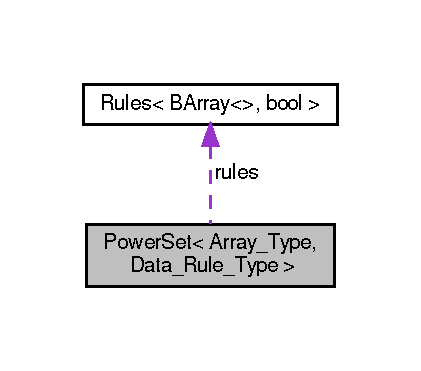
\includegraphics[width=202pt]{class_power_set__coll__graph}
\end{center}
\end{figure}
\doxysubsection*{Public Member Functions}
\begin{DoxyCompactItemize}
\item 
void \mbox{\hyperlink{class_power_set_a8eefc9606c6339938a8d9adcd0d7e153}{init\+\_\+support}} ()
\item 
void \mbox{\hyperlink{class_power_set_ad3b707294498105b2cc1a04017cc96d2}{calc}} ()
\item 
void \mbox{\hyperlink{class_power_set_af7d11e5c37d3a69b5e526c67632c646c}{reset}} (size\+\_\+t N\+\_\+, size\+\_\+t M\+\_\+)
\end{DoxyCompactItemize}
\begin{Indent}\textbf{ Construct and destroy a Power\+Set object}\par
\begin{DoxyCompactItemize}
\item 
\mbox{\hyperlink{class_power_set_a095815ccc44c88e0da73d92c6b5cf5f3}{Power\+Set}} ()
\item 
\mbox{\hyperlink{class_power_set_ad25c0d16623800a432a953cd9953c644}{Power\+Set}} (size\+\_\+t N\+\_\+, size\+\_\+t M\+\_\+)
\item 
\mbox{\hyperlink{class_power_set_acc20a68ff11aa1891d9a0676ed50808f}{Power\+Set}} (const Array\+\_\+\+Type \&array)
\item 
\mbox{\hyperlink{class_power_set_a89a176c9517e81a066adffad3c46aba5}{$\sim$\+Power\+Set}} ()
\end{DoxyCompactItemize}
\end{Indent}
\begin{Indent}\textbf{ Wrappers for the $<$tt$>$Rules$<$/tt$>$ member.}\par
{\em These will add rules to the model, which are shared by the support and the actual counter function. }\begin{DoxyCompactItemize}
\item 
void \mbox{\hyperlink{class_power_set_a76d15305bc98b5c03904398e81457368}{add\+\_\+rule}} (\mbox{\hyperlink{class_rule}{Rule}}$<$ Array\+\_\+\+Type, \mbox{\hyperlink{model-meat_8hpp_ab662732874257647dc631846c67da586}{Data\+\_\+\+Rule\+\_\+\+Type}} $>$ rule)
\item 
void \mbox{\hyperlink{class_power_set_a3c9f2ab6184688d9879c6555b4c3e813}{add\+\_\+rule}} (\mbox{\hyperlink{typedefs_8hpp_a940d68f006f1ffee7f5b207bf61aefe4}{Rule\+\_\+fun\+\_\+type}}$<$ Array\+\_\+\+Type, \mbox{\hyperlink{model-meat_8hpp_ab662732874257647dc631846c67da586}{Data\+\_\+\+Rule\+\_\+\+Type}} $>$ \mbox{\hyperlink{model-meat_8hpp_a2648076475c82f8bfed17e9c46b36f68}{count\+\_\+fun\+\_\+}}, \mbox{\hyperlink{model-meat_8hpp_ab662732874257647dc631846c67da586}{Data\+\_\+\+Rule\+\_\+\+Type}} \mbox{\hyperlink{model-meat_8hpp_add877eae455a35aea9e5c7de9c6f2dbb}{data\+\_\+}})
\end{DoxyCompactItemize}
\end{Indent}
\begin{Indent}\textbf{ Getter functions}\par
\begin{DoxyCompactItemize}
\item 
const std\+::vector$<$ Array\+\_\+\+Type $>$ $\ast$ \mbox{\hyperlink{class_power_set_a99cf1aa56e63a16c023bf7057b0b9288}{get\+\_\+data\+\_\+ptr}} () const
\item 
std\+::vector$<$ Array\+\_\+\+Type $>$ \mbox{\hyperlink{class_power_set_a4de44631d9a7967db4dd791d42166115}{get\+\_\+data}} () const
\item 
std\+::vector$<$ Array\+\_\+\+Type $>$\+::iterator \mbox{\hyperlink{class_power_set_abed9d58db924366d8a38baf168131fc3}{begin}} ()
\item 
std\+::vector$<$ Array\+\_\+\+Type $>$\+::iterator \mbox{\hyperlink{class_power_set_ac734ed684aa314b722a05d423c607a38}{end}} ()
\item 
std\+::size\+\_\+t \mbox{\hyperlink{class_power_set_a9a92b7c43517e11f3245a7ae89a578ef}{size}} () const \mbox{\hyperlink{counters-meat_8hpp_ae763aeff9df78ca7be5f904fa4bbdc09}{noexcept}}
\item 
const Array\+\_\+\+Type \& \mbox{\hyperlink{class_power_set_ab237095aa18a4997a3cec61d64cfe1dc}{operator\mbox{[}$\,$\mbox{]}}} (const size\+\_\+t \&\mbox{\hyperlink{model-meat_8hpp_a981162f997bbddbdcaf8234da58a6094}{i}}) const
\end{DoxyCompactItemize}
\end{Indent}
\doxysubsection*{Public Attributes}
\begin{DoxyCompactItemize}
\item 
Array\+\_\+\+Type \mbox{\hyperlink{class_power_set_a367db2c97e0301dd0dd78e5e4b458d34}{Empty\+Array}}
\item 
std\+::vector$<$ Array\+\_\+\+Type $>$ \mbox{\hyperlink{class_power_set_af456c157d157692ba5890c549c51af75}{data}}
\item 
\mbox{\hyperlink{class_rules}{Rules}}$<$ Array\+\_\+\+Type, \mbox{\hyperlink{model-meat_8hpp_ab662732874257647dc631846c67da586}{Data\+\_\+\+Rule\+\_\+\+Type}} $>$ $\ast$ \mbox{\hyperlink{class_power_set_afa542ecc31858c8644d1e76078eb1713}{rules}}
\item 
size\+\_\+t \mbox{\hyperlink{class_power_set_a0d23e8e17d30ac0dcb740634bf817ac7}{N}}
\item 
size\+\_\+t \mbox{\hyperlink{class_power_set_abfbefec5e1bbda8282ca3fcba2bb4b8e}{M}}
\item 
bool \mbox{\hyperlink{class_power_set_a08b6baf1e244e023d997ddaecbc2116f}{rules\+\_\+deleted}} = false
\item 
std\+::vector$<$ size\+\_\+t $>$ \mbox{\hyperlink{class_power_set_a1ccab9487dde1f4d1961983eb28c0976}{coordinates\+\_\+free}}
\item 
std\+::vector$<$ size\+\_\+t $>$ \mbox{\hyperlink{class_power_set_ad9e1a542a0234e3f943611de2bcab51a}{coordinates\+\_\+locked}}
\item 
size\+\_\+t \mbox{\hyperlink{class_power_set_a017d35750d824f8e9ce7e03b996c4d4c}{n\+\_\+free}}
\item 
size\+\_\+t \mbox{\hyperlink{class_power_set_a690b4321cd83063d5b78d192993864b2}{n\+\_\+locked}}
\end{DoxyCompactItemize}


\doxysubsection{Detailed Description}
\subsubsection*{template$<$typename Array\+\_\+\+Type = BArray$<$$>$, typename Data\+\_\+\+Rule\+\_\+\+Type = bool$>$\newline
class Power\+Set$<$ Array\+\_\+\+Type, Data\+\_\+\+Rule\+\_\+\+Type $>$}

Powerset of a binary array. 


\begin{DoxyTemplParams}{Template Parameters}
{\em Array\+\_\+\+Type} & \\
\hline
{\em Data\+\_\+\+Rule\+\_\+\+Type} & \\
\hline
\end{DoxyTemplParams}


Definition at line 11 of file powerset-\/bones.\+hpp.



\doxysubsection{Constructor \& Destructor Documentation}
\mbox{\Hypertarget{class_power_set_a095815ccc44c88e0da73d92c6b5cf5f3}\label{class_power_set_a095815ccc44c88e0da73d92c6b5cf5f3}} 
\index{PowerSet$<$ Array\_Type, Data\_Rule\_Type $>$@{PowerSet$<$ Array\_Type, Data\_Rule\_Type $>$}!PowerSet@{PowerSet}}
\index{PowerSet@{PowerSet}!PowerSet$<$ Array\_Type, Data\_Rule\_Type $>$@{PowerSet$<$ Array\_Type, Data\_Rule\_Type $>$}}
\doxysubsubsection{\texorpdfstring{PowerSet()}{PowerSet()}\hspace{0.1cm}{\footnotesize\ttfamily [1/3]}}
{\footnotesize\ttfamily template$<$typename Array\+\_\+\+Type  = BArray$<$$>$, typename Data\+\_\+\+Rule\+\_\+\+Type  = bool$>$ \\
\mbox{\hyperlink{class_power_set}{Power\+Set}}$<$ Array\+\_\+\+Type, \mbox{\hyperlink{model-meat_8hpp_ab662732874257647dc631846c67da586}{Data\+\_\+\+Rule\+\_\+\+Type}} $>$\+::\mbox{\hyperlink{class_power_set}{Power\+Set}} (\begin{DoxyParamCaption}{ }\end{DoxyParamCaption})\hspace{0.3cm}{\ttfamily [inline]}}



Definition at line 36 of file powerset-\/bones.\+hpp.

\mbox{\Hypertarget{class_power_set_ad25c0d16623800a432a953cd9953c644}\label{class_power_set_ad25c0d16623800a432a953cd9953c644}} 
\index{PowerSet$<$ Array\_Type, Data\_Rule\_Type $>$@{PowerSet$<$ Array\_Type, Data\_Rule\_Type $>$}!PowerSet@{PowerSet}}
\index{PowerSet@{PowerSet}!PowerSet$<$ Array\_Type, Data\_Rule\_Type $>$@{PowerSet$<$ Array\_Type, Data\_Rule\_Type $>$}}
\doxysubsubsection{\texorpdfstring{PowerSet()}{PowerSet()}\hspace{0.1cm}{\footnotesize\ttfamily [2/3]}}
{\footnotesize\ttfamily template$<$typename Array\+\_\+\+Type  = BArray$<$$>$, typename Data\+\_\+\+Rule\+\_\+\+Type  = bool$>$ \\
\mbox{\hyperlink{class_power_set}{Power\+Set}}$<$ Array\+\_\+\+Type, \mbox{\hyperlink{model-meat_8hpp_ab662732874257647dc631846c67da586}{Data\+\_\+\+Rule\+\_\+\+Type}} $>$\+::\mbox{\hyperlink{class_power_set}{Power\+Set}} (\begin{DoxyParamCaption}\item[{size\+\_\+t}]{N\+\_\+,  }\item[{size\+\_\+t}]{M\+\_\+ }\end{DoxyParamCaption})\hspace{0.3cm}{\ttfamily [inline]}}



Definition at line 38 of file powerset-\/bones.\+hpp.

\mbox{\Hypertarget{class_power_set_acc20a68ff11aa1891d9a0676ed50808f}\label{class_power_set_acc20a68ff11aa1891d9a0676ed50808f}} 
\index{PowerSet$<$ Array\_Type, Data\_Rule\_Type $>$@{PowerSet$<$ Array\_Type, Data\_Rule\_Type $>$}!PowerSet@{PowerSet}}
\index{PowerSet@{PowerSet}!PowerSet$<$ Array\_Type, Data\_Rule\_Type $>$@{PowerSet$<$ Array\_Type, Data\_Rule\_Type $>$}}
\doxysubsubsection{\texorpdfstring{PowerSet()}{PowerSet()}\hspace{0.1cm}{\footnotesize\ttfamily [3/3]}}
{\footnotesize\ttfamily template$<$typename Array\+\_\+\+Type , typename Data\+\_\+\+Rule\+\_\+\+Type $>$ \\
\mbox{\hyperlink{class_power_set}{Power\+Set}}$<$ Array\+\_\+\+Type, \mbox{\hyperlink{model-meat_8hpp_ab662732874257647dc631846c67da586}{Data\+\_\+\+Rule\+\_\+\+Type}} $>$\+::\mbox{\hyperlink{class_power_set}{Power\+Set}} (\begin{DoxyParamCaption}\item[{const Array\+\_\+\+Type \&}]{array }\end{DoxyParamCaption})\hspace{0.3cm}{\ttfamily [inline]}}



Definition at line 5 of file powerset-\/meat.\+hpp.

\mbox{\Hypertarget{class_power_set_a89a176c9517e81a066adffad3c46aba5}\label{class_power_set_a89a176c9517e81a066adffad3c46aba5}} 
\index{PowerSet$<$ Array\_Type, Data\_Rule\_Type $>$@{PowerSet$<$ Array\_Type, Data\_Rule\_Type $>$}!````~PowerSet@{$\sim$PowerSet}}
\index{````~PowerSet@{$\sim$PowerSet}!PowerSet$<$ Array\_Type, Data\_Rule\_Type $>$@{PowerSet$<$ Array\_Type, Data\_Rule\_Type $>$}}
\doxysubsubsection{\texorpdfstring{$\sim$PowerSet()}{~PowerSet()}}
{\footnotesize\ttfamily template$<$typename Array\+\_\+\+Type , typename Data\+\_\+\+Rule\+\_\+\+Type $>$ \\
\mbox{\hyperlink{class_power_set}{Power\+Set}}$<$ Array\+\_\+\+Type, \mbox{\hyperlink{model-meat_8hpp_ab662732874257647dc631846c67da586}{Data\+\_\+\+Rule\+\_\+\+Type}} $>$\+::$\sim$\mbox{\hyperlink{class_power_set}{Power\+Set}}\hspace{0.3cm}{\ttfamily [inline]}}



Definition at line 13 of file powerset-\/meat.\+hpp.



\doxysubsection{Member Function Documentation}
\mbox{\Hypertarget{class_power_set_a76d15305bc98b5c03904398e81457368}\label{class_power_set_a76d15305bc98b5c03904398e81457368}} 
\index{PowerSet$<$ Array\_Type, Data\_Rule\_Type $>$@{PowerSet$<$ Array\_Type, Data\_Rule\_Type $>$}!add\_rule@{add\_rule}}
\index{add\_rule@{add\_rule}!PowerSet$<$ Array\_Type, Data\_Rule\_Type $>$@{PowerSet$<$ Array\_Type, Data\_Rule\_Type $>$}}
\doxysubsubsection{\texorpdfstring{add\_rule()}{add\_rule()}\hspace{0.1cm}{\footnotesize\ttfamily [1/2]}}
{\footnotesize\ttfamily template$<$typename Array\+\_\+\+Type , typename Data\+\_\+\+Rule\+\_\+\+Type $>$ \\
void \mbox{\hyperlink{class_power_set}{Power\+Set}}$<$ Array\+\_\+\+Type, \mbox{\hyperlink{model-meat_8hpp_ab662732874257647dc631846c67da586}{Data\+\_\+\+Rule\+\_\+\+Type}} $>$\+::add\+\_\+rule (\begin{DoxyParamCaption}\item[{\mbox{\hyperlink{class_rule}{Rule}}$<$ Array\+\_\+\+Type, \mbox{\hyperlink{model-meat_8hpp_ab662732874257647dc631846c67da586}{Data\+\_\+\+Rule\+\_\+\+Type}} $>$}]{rule }\end{DoxyParamCaption})\hspace{0.3cm}{\ttfamily [inline]}}



Definition at line 173 of file powerset-\/meat.\+hpp.

\mbox{\Hypertarget{class_power_set_a3c9f2ab6184688d9879c6555b4c3e813}\label{class_power_set_a3c9f2ab6184688d9879c6555b4c3e813}} 
\index{PowerSet$<$ Array\_Type, Data\_Rule\_Type $>$@{PowerSet$<$ Array\_Type, Data\_Rule\_Type $>$}!add\_rule@{add\_rule}}
\index{add\_rule@{add\_rule}!PowerSet$<$ Array\_Type, Data\_Rule\_Type $>$@{PowerSet$<$ Array\_Type, Data\_Rule\_Type $>$}}
\doxysubsubsection{\texorpdfstring{add\_rule()}{add\_rule()}\hspace{0.1cm}{\footnotesize\ttfamily [2/2]}}
{\footnotesize\ttfamily template$<$typename Array\+\_\+\+Type , typename Data\+\_\+\+Rule\+\_\+\+Type $>$ \\
void \mbox{\hyperlink{class_power_set}{Power\+Set}}$<$ Array\+\_\+\+Type, \mbox{\hyperlink{model-meat_8hpp_ab662732874257647dc631846c67da586}{Data\+\_\+\+Rule\+\_\+\+Type}} $>$\+::add\+\_\+rule (\begin{DoxyParamCaption}\item[{\mbox{\hyperlink{typedefs_8hpp_a940d68f006f1ffee7f5b207bf61aefe4}{Rule\+\_\+fun\+\_\+type}}$<$ Array\+\_\+\+Type, \mbox{\hyperlink{model-meat_8hpp_ab662732874257647dc631846c67da586}{Data\+\_\+\+Rule\+\_\+\+Type}} $>$}]{count\+\_\+fun\+\_\+,  }\item[{\mbox{\hyperlink{model-meat_8hpp_ab662732874257647dc631846c67da586}{Data\+\_\+\+Rule\+\_\+\+Type}}}]{data\+\_\+ }\end{DoxyParamCaption})\hspace{0.3cm}{\ttfamily [inline]}}



Definition at line 182 of file powerset-\/meat.\+hpp.

\mbox{\Hypertarget{class_power_set_abed9d58db924366d8a38baf168131fc3}\label{class_power_set_abed9d58db924366d8a38baf168131fc3}} 
\index{PowerSet$<$ Array\_Type, Data\_Rule\_Type $>$@{PowerSet$<$ Array\_Type, Data\_Rule\_Type $>$}!begin@{begin}}
\index{begin@{begin}!PowerSet$<$ Array\_Type, Data\_Rule\_Type $>$@{PowerSet$<$ Array\_Type, Data\_Rule\_Type $>$}}
\doxysubsubsection{\texorpdfstring{begin()}{begin()}}
{\footnotesize\ttfamily template$<$typename Array\+\_\+\+Type  = BArray$<$$>$, typename Data\+\_\+\+Rule\+\_\+\+Type  = bool$>$ \\
std\+::vector$<$ Array\+\_\+\+Type $>$\+::iterator \mbox{\hyperlink{class_power_set}{Power\+Set}}$<$ Array\+\_\+\+Type, \mbox{\hyperlink{model-meat_8hpp_ab662732874257647dc631846c67da586}{Data\+\_\+\+Rule\+\_\+\+Type}} $>$\+::begin (\begin{DoxyParamCaption}{ }\end{DoxyParamCaption})\hspace{0.3cm}{\ttfamily [inline]}}



Definition at line 68 of file powerset-\/bones.\+hpp.

\mbox{\Hypertarget{class_power_set_ad3b707294498105b2cc1a04017cc96d2}\label{class_power_set_ad3b707294498105b2cc1a04017cc96d2}} 
\index{PowerSet$<$ Array\_Type, Data\_Rule\_Type $>$@{PowerSet$<$ Array\_Type, Data\_Rule\_Type $>$}!calc@{calc}}
\index{calc@{calc}!PowerSet$<$ Array\_Type, Data\_Rule\_Type $>$@{PowerSet$<$ Array\_Type, Data\_Rule\_Type $>$}}
\doxysubsubsection{\texorpdfstring{calc()}{calc()}}
{\footnotesize\ttfamily template$<$typename Array\+\_\+\+Type , typename Data\+\_\+\+Rule\+\_\+\+Type $>$ \\
void \mbox{\hyperlink{class_power_set}{Power\+Set}}$<$ Array\+\_\+\+Type, \mbox{\hyperlink{model-meat_8hpp_ab662732874257647dc631846c67da586}{Data\+\_\+\+Rule\+\_\+\+Type}} $>$\+::calc\hspace{0.3cm}{\ttfamily [inline]}}



Definition at line 144 of file powerset-\/meat.\+hpp.

\mbox{\Hypertarget{class_power_set_ac734ed684aa314b722a05d423c607a38}\label{class_power_set_ac734ed684aa314b722a05d423c607a38}} 
\index{PowerSet$<$ Array\_Type, Data\_Rule\_Type $>$@{PowerSet$<$ Array\_Type, Data\_Rule\_Type $>$}!end@{end}}
\index{end@{end}!PowerSet$<$ Array\_Type, Data\_Rule\_Type $>$@{PowerSet$<$ Array\_Type, Data\_Rule\_Type $>$}}
\doxysubsubsection{\texorpdfstring{end()}{end()}}
{\footnotesize\ttfamily template$<$typename Array\+\_\+\+Type  = BArray$<$$>$, typename Data\+\_\+\+Rule\+\_\+\+Type  = bool$>$ \\
std\+::vector$<$ Array\+\_\+\+Type $>$\+::iterator \mbox{\hyperlink{class_power_set}{Power\+Set}}$<$ Array\+\_\+\+Type, \mbox{\hyperlink{model-meat_8hpp_ab662732874257647dc631846c67da586}{Data\+\_\+\+Rule\+\_\+\+Type}} $>$\+::end (\begin{DoxyParamCaption}{ }\end{DoxyParamCaption})\hspace{0.3cm}{\ttfamily [inline]}}



Definition at line 69 of file powerset-\/bones.\+hpp.

\mbox{\Hypertarget{class_power_set_a4de44631d9a7967db4dd791d42166115}\label{class_power_set_a4de44631d9a7967db4dd791d42166115}} 
\index{PowerSet$<$ Array\_Type, Data\_Rule\_Type $>$@{PowerSet$<$ Array\_Type, Data\_Rule\_Type $>$}!get\_data@{get\_data}}
\index{get\_data@{get\_data}!PowerSet$<$ Array\_Type, Data\_Rule\_Type $>$@{PowerSet$<$ Array\_Type, Data\_Rule\_Type $>$}}
\doxysubsubsection{\texorpdfstring{get\_data()}{get\_data()}}
{\footnotesize\ttfamily template$<$typename Array\+\_\+\+Type  = BArray$<$$>$, typename Data\+\_\+\+Rule\+\_\+\+Type  = bool$>$ \\
std\+::vector$<$ Array\+\_\+\+Type $>$ \mbox{\hyperlink{class_power_set}{Power\+Set}}$<$ Array\+\_\+\+Type, \mbox{\hyperlink{model-meat_8hpp_ab662732874257647dc631846c67da586}{Data\+\_\+\+Rule\+\_\+\+Type}} $>$\+::get\+\_\+data (\begin{DoxyParamCaption}{ }\end{DoxyParamCaption}) const\hspace{0.3cm}{\ttfamily [inline]}}



Definition at line 67 of file powerset-\/bones.\+hpp.

\mbox{\Hypertarget{class_power_set_a99cf1aa56e63a16c023bf7057b0b9288}\label{class_power_set_a99cf1aa56e63a16c023bf7057b0b9288}} 
\index{PowerSet$<$ Array\_Type, Data\_Rule\_Type $>$@{PowerSet$<$ Array\_Type, Data\_Rule\_Type $>$}!get\_data\_ptr@{get\_data\_ptr}}
\index{get\_data\_ptr@{get\_data\_ptr}!PowerSet$<$ Array\_Type, Data\_Rule\_Type $>$@{PowerSet$<$ Array\_Type, Data\_Rule\_Type $>$}}
\doxysubsubsection{\texorpdfstring{get\_data\_ptr()}{get\_data\_ptr()}}
{\footnotesize\ttfamily template$<$typename Array\+\_\+\+Type  = BArray$<$$>$, typename Data\+\_\+\+Rule\+\_\+\+Type  = bool$>$ \\
const std\+::vector$<$ Array\+\_\+\+Type $>$$\ast$ \mbox{\hyperlink{class_power_set}{Power\+Set}}$<$ Array\+\_\+\+Type, \mbox{\hyperlink{model-meat_8hpp_ab662732874257647dc631846c67da586}{Data\+\_\+\+Rule\+\_\+\+Type}} $>$\+::get\+\_\+data\+\_\+ptr (\begin{DoxyParamCaption}{ }\end{DoxyParamCaption}) const\hspace{0.3cm}{\ttfamily [inline]}}



Definition at line 66 of file powerset-\/bones.\+hpp.

\mbox{\Hypertarget{class_power_set_a8eefc9606c6339938a8d9adcd0d7e153}\label{class_power_set_a8eefc9606c6339938a8d9adcd0d7e153}} 
\index{PowerSet$<$ Array\_Type, Data\_Rule\_Type $>$@{PowerSet$<$ Array\_Type, Data\_Rule\_Type $>$}!init\_support@{init\_support}}
\index{init\_support@{init\_support}!PowerSet$<$ Array\_Type, Data\_Rule\_Type $>$@{PowerSet$<$ Array\_Type, Data\_Rule\_Type $>$}}
\doxysubsubsection{\texorpdfstring{init\_support()}{init\_support()}}
{\footnotesize\ttfamily template$<$typename Array\+\_\+\+Type , typename Data\+\_\+\+Rule\+\_\+\+Type $>$ \\
void \mbox{\hyperlink{class_power_set}{Power\+Set}}$<$ Array\+\_\+\+Type, \mbox{\hyperlink{model-meat_8hpp_ab662732874257647dc631846c67da586}{Data\+\_\+\+Rule\+\_\+\+Type}} $>$\+::init\+\_\+support\hspace{0.3cm}{\ttfamily [inline]}}



Definition at line 19 of file powerset-\/meat.\+hpp.

\mbox{\Hypertarget{class_power_set_ab237095aa18a4997a3cec61d64cfe1dc}\label{class_power_set_ab237095aa18a4997a3cec61d64cfe1dc}} 
\index{PowerSet$<$ Array\_Type, Data\_Rule\_Type $>$@{PowerSet$<$ Array\_Type, Data\_Rule\_Type $>$}!operator\mbox{[}\mbox{]}@{operator[]}}
\index{operator\mbox{[}\mbox{]}@{operator[]}!PowerSet$<$ Array\_Type, Data\_Rule\_Type $>$@{PowerSet$<$ Array\_Type, Data\_Rule\_Type $>$}}
\doxysubsubsection{\texorpdfstring{operator[]()}{operator[]()}}
{\footnotesize\ttfamily template$<$typename Array\+\_\+\+Type  = BArray$<$$>$, typename Data\+\_\+\+Rule\+\_\+\+Type  = bool$>$ \\
const Array\+\_\+\+Type\& \mbox{\hyperlink{class_power_set}{Power\+Set}}$<$ Array\+\_\+\+Type, \mbox{\hyperlink{model-meat_8hpp_ab662732874257647dc631846c67da586}{Data\+\_\+\+Rule\+\_\+\+Type}} $>$\+::operator\mbox{[}$\,$\mbox{]} (\begin{DoxyParamCaption}\item[{const size\+\_\+t \&}]{i }\end{DoxyParamCaption}) const\hspace{0.3cm}{\ttfamily [inline]}}



Definition at line 71 of file powerset-\/bones.\+hpp.

\mbox{\Hypertarget{class_power_set_af7d11e5c37d3a69b5e526c67632c646c}\label{class_power_set_af7d11e5c37d3a69b5e526c67632c646c}} 
\index{PowerSet$<$ Array\_Type, Data\_Rule\_Type $>$@{PowerSet$<$ Array\_Type, Data\_Rule\_Type $>$}!reset@{reset}}
\index{reset@{reset}!PowerSet$<$ Array\_Type, Data\_Rule\_Type $>$@{PowerSet$<$ Array\_Type, Data\_Rule\_Type $>$}}
\doxysubsubsection{\texorpdfstring{reset()}{reset()}}
{\footnotesize\ttfamily template$<$typename Array\+\_\+\+Type , typename Data\+\_\+\+Rule\+\_\+\+Type $>$ \\
void \mbox{\hyperlink{class_power_set}{Power\+Set}}$<$ Array\+\_\+\+Type, \mbox{\hyperlink{model-meat_8hpp_ab662732874257647dc631846c67da586}{Data\+\_\+\+Rule\+\_\+\+Type}} $>$\+::reset (\begin{DoxyParamCaption}\item[{size\+\_\+t}]{N\+\_\+,  }\item[{size\+\_\+t}]{M\+\_\+ }\end{DoxyParamCaption})\hspace{0.3cm}{\ttfamily [inline]}}



Definition at line 160 of file powerset-\/meat.\+hpp.

\mbox{\Hypertarget{class_power_set_a9a92b7c43517e11f3245a7ae89a578ef}\label{class_power_set_a9a92b7c43517e11f3245a7ae89a578ef}} 
\index{PowerSet$<$ Array\_Type, Data\_Rule\_Type $>$@{PowerSet$<$ Array\_Type, Data\_Rule\_Type $>$}!size@{size}}
\index{size@{size}!PowerSet$<$ Array\_Type, Data\_Rule\_Type $>$@{PowerSet$<$ Array\_Type, Data\_Rule\_Type $>$}}
\doxysubsubsection{\texorpdfstring{size()}{size()}}
{\footnotesize\ttfamily template$<$typename Array\+\_\+\+Type  = BArray$<$$>$, typename Data\+\_\+\+Rule\+\_\+\+Type  = bool$>$ \\
std\+::size\+\_\+t \mbox{\hyperlink{class_power_set}{Power\+Set}}$<$ Array\+\_\+\+Type, \mbox{\hyperlink{model-meat_8hpp_ab662732874257647dc631846c67da586}{Data\+\_\+\+Rule\+\_\+\+Type}} $>$\+::size (\begin{DoxyParamCaption}{ }\end{DoxyParamCaption}) const\hspace{0.3cm}{\ttfamily [inline]}, {\ttfamily [noexcept]}}



Definition at line 70 of file powerset-\/bones.\+hpp.



\doxysubsection{Member Data Documentation}
\mbox{\Hypertarget{class_power_set_a1ccab9487dde1f4d1961983eb28c0976}\label{class_power_set_a1ccab9487dde1f4d1961983eb28c0976}} 
\index{PowerSet$<$ Array\_Type, Data\_Rule\_Type $>$@{PowerSet$<$ Array\_Type, Data\_Rule\_Type $>$}!coordinates\_free@{coordinates\_free}}
\index{coordinates\_free@{coordinates\_free}!PowerSet$<$ Array\_Type, Data\_Rule\_Type $>$@{PowerSet$<$ Array\_Type, Data\_Rule\_Type $>$}}
\doxysubsubsection{\texorpdfstring{coordinates\_free}{coordinates\_free}}
{\footnotesize\ttfamily template$<$typename Array\+\_\+\+Type  = BArray$<$$>$, typename Data\+\_\+\+Rule\+\_\+\+Type  = bool$>$ \\
std\+::vector$<$ size\+\_\+t $>$ \mbox{\hyperlink{class_power_set}{Power\+Set}}$<$ Array\+\_\+\+Type, \mbox{\hyperlink{model-meat_8hpp_ab662732874257647dc631846c67da586}{Data\+\_\+\+Rule\+\_\+\+Type}} $>$\+::coordinates\+\_\+free}



Definition at line 26 of file powerset-\/bones.\+hpp.

\mbox{\Hypertarget{class_power_set_ad9e1a542a0234e3f943611de2bcab51a}\label{class_power_set_ad9e1a542a0234e3f943611de2bcab51a}} 
\index{PowerSet$<$ Array\_Type, Data\_Rule\_Type $>$@{PowerSet$<$ Array\_Type, Data\_Rule\_Type $>$}!coordinates\_locked@{coordinates\_locked}}
\index{coordinates\_locked@{coordinates\_locked}!PowerSet$<$ Array\_Type, Data\_Rule\_Type $>$@{PowerSet$<$ Array\_Type, Data\_Rule\_Type $>$}}
\doxysubsubsection{\texorpdfstring{coordinates\_locked}{coordinates\_locked}}
{\footnotesize\ttfamily template$<$typename Array\+\_\+\+Type  = BArray$<$$>$, typename Data\+\_\+\+Rule\+\_\+\+Type  = bool$>$ \\
std\+::vector$<$ size\+\_\+t $>$ \mbox{\hyperlink{class_power_set}{Power\+Set}}$<$ Array\+\_\+\+Type, \mbox{\hyperlink{model-meat_8hpp_ab662732874257647dc631846c67da586}{Data\+\_\+\+Rule\+\_\+\+Type}} $>$\+::coordinates\+\_\+locked}



Definition at line 27 of file powerset-\/bones.\+hpp.

\mbox{\Hypertarget{class_power_set_af456c157d157692ba5890c549c51af75}\label{class_power_set_af456c157d157692ba5890c549c51af75}} 
\index{PowerSet$<$ Array\_Type, Data\_Rule\_Type $>$@{PowerSet$<$ Array\_Type, Data\_Rule\_Type $>$}!data@{data}}
\index{data@{data}!PowerSet$<$ Array\_Type, Data\_Rule\_Type $>$@{PowerSet$<$ Array\_Type, Data\_Rule\_Type $>$}}
\doxysubsubsection{\texorpdfstring{data}{data}}
{\footnotesize\ttfamily template$<$typename Array\+\_\+\+Type  = BArray$<$$>$, typename Data\+\_\+\+Rule\+\_\+\+Type  = bool$>$ \\
std\+::vector$<$ Array\+\_\+\+Type $>$ \mbox{\hyperlink{class_power_set}{Power\+Set}}$<$ Array\+\_\+\+Type, \mbox{\hyperlink{model-meat_8hpp_ab662732874257647dc631846c67da586}{Data\+\_\+\+Rule\+\_\+\+Type}} $>$\+::data}



Definition at line 19 of file powerset-\/bones.\+hpp.

\mbox{\Hypertarget{class_power_set_a367db2c97e0301dd0dd78e5e4b458d34}\label{class_power_set_a367db2c97e0301dd0dd78e5e4b458d34}} 
\index{PowerSet$<$ Array\_Type, Data\_Rule\_Type $>$@{PowerSet$<$ Array\_Type, Data\_Rule\_Type $>$}!EmptyArray@{EmptyArray}}
\index{EmptyArray@{EmptyArray}!PowerSet$<$ Array\_Type, Data\_Rule\_Type $>$@{PowerSet$<$ Array\_Type, Data\_Rule\_Type $>$}}
\doxysubsubsection{\texorpdfstring{EmptyArray}{EmptyArray}}
{\footnotesize\ttfamily template$<$typename Array\+\_\+\+Type  = BArray$<$$>$, typename Data\+\_\+\+Rule\+\_\+\+Type  = bool$>$ \\
Array\+\_\+\+Type \mbox{\hyperlink{class_power_set}{Power\+Set}}$<$ Array\+\_\+\+Type, \mbox{\hyperlink{model-meat_8hpp_ab662732874257647dc631846c67da586}{Data\+\_\+\+Rule\+\_\+\+Type}} $>$\+::Empty\+Array}



Definition at line 18 of file powerset-\/bones.\+hpp.

\mbox{\Hypertarget{class_power_set_abfbefec5e1bbda8282ca3fcba2bb4b8e}\label{class_power_set_abfbefec5e1bbda8282ca3fcba2bb4b8e}} 
\index{PowerSet$<$ Array\_Type, Data\_Rule\_Type $>$@{PowerSet$<$ Array\_Type, Data\_Rule\_Type $>$}!M@{M}}
\index{M@{M}!PowerSet$<$ Array\_Type, Data\_Rule\_Type $>$@{PowerSet$<$ Array\_Type, Data\_Rule\_Type $>$}}
\doxysubsubsection{\texorpdfstring{M}{M}}
{\footnotesize\ttfamily template$<$typename Array\+\_\+\+Type  = BArray$<$$>$, typename Data\+\_\+\+Rule\+\_\+\+Type  = bool$>$ \\
size\+\_\+t \mbox{\hyperlink{class_power_set}{Power\+Set}}$<$ Array\+\_\+\+Type, \mbox{\hyperlink{model-meat_8hpp_ab662732874257647dc631846c67da586}{Data\+\_\+\+Rule\+\_\+\+Type}} $>$\+::M}



Definition at line 22 of file powerset-\/bones.\+hpp.

\mbox{\Hypertarget{class_power_set_a0d23e8e17d30ac0dcb740634bf817ac7}\label{class_power_set_a0d23e8e17d30ac0dcb740634bf817ac7}} 
\index{PowerSet$<$ Array\_Type, Data\_Rule\_Type $>$@{PowerSet$<$ Array\_Type, Data\_Rule\_Type $>$}!N@{N}}
\index{N@{N}!PowerSet$<$ Array\_Type, Data\_Rule\_Type $>$@{PowerSet$<$ Array\_Type, Data\_Rule\_Type $>$}}
\doxysubsubsection{\texorpdfstring{N}{N}}
{\footnotesize\ttfamily template$<$typename Array\+\_\+\+Type  = BArray$<$$>$, typename Data\+\_\+\+Rule\+\_\+\+Type  = bool$>$ \\
size\+\_\+t \mbox{\hyperlink{class_power_set}{Power\+Set}}$<$ Array\+\_\+\+Type, \mbox{\hyperlink{model-meat_8hpp_ab662732874257647dc631846c67da586}{Data\+\_\+\+Rule\+\_\+\+Type}} $>$\+::N}



Definition at line 22 of file powerset-\/bones.\+hpp.

\mbox{\Hypertarget{class_power_set_a017d35750d824f8e9ce7e03b996c4d4c}\label{class_power_set_a017d35750d824f8e9ce7e03b996c4d4c}} 
\index{PowerSet$<$ Array\_Type, Data\_Rule\_Type $>$@{PowerSet$<$ Array\_Type, Data\_Rule\_Type $>$}!n\_free@{n\_free}}
\index{n\_free@{n\_free}!PowerSet$<$ Array\_Type, Data\_Rule\_Type $>$@{PowerSet$<$ Array\_Type, Data\_Rule\_Type $>$}}
\doxysubsubsection{\texorpdfstring{n\_free}{n\_free}}
{\footnotesize\ttfamily template$<$typename Array\+\_\+\+Type  = BArray$<$$>$, typename Data\+\_\+\+Rule\+\_\+\+Type  = bool$>$ \\
size\+\_\+t \mbox{\hyperlink{class_power_set}{Power\+Set}}$<$ Array\+\_\+\+Type, \mbox{\hyperlink{model-meat_8hpp_ab662732874257647dc631846c67da586}{Data\+\_\+\+Rule\+\_\+\+Type}} $>$\+::n\+\_\+free}



Definition at line 28 of file powerset-\/bones.\+hpp.

\mbox{\Hypertarget{class_power_set_a690b4321cd83063d5b78d192993864b2}\label{class_power_set_a690b4321cd83063d5b78d192993864b2}} 
\index{PowerSet$<$ Array\_Type, Data\_Rule\_Type $>$@{PowerSet$<$ Array\_Type, Data\_Rule\_Type $>$}!n\_locked@{n\_locked}}
\index{n\_locked@{n\_locked}!PowerSet$<$ Array\_Type, Data\_Rule\_Type $>$@{PowerSet$<$ Array\_Type, Data\_Rule\_Type $>$}}
\doxysubsubsection{\texorpdfstring{n\_locked}{n\_locked}}
{\footnotesize\ttfamily template$<$typename Array\+\_\+\+Type  = BArray$<$$>$, typename Data\+\_\+\+Rule\+\_\+\+Type  = bool$>$ \\
size\+\_\+t \mbox{\hyperlink{class_power_set}{Power\+Set}}$<$ Array\+\_\+\+Type, \mbox{\hyperlink{model-meat_8hpp_ab662732874257647dc631846c67da586}{Data\+\_\+\+Rule\+\_\+\+Type}} $>$\+::n\+\_\+locked}



Definition at line 29 of file powerset-\/bones.\+hpp.

\mbox{\Hypertarget{class_power_set_afa542ecc31858c8644d1e76078eb1713}\label{class_power_set_afa542ecc31858c8644d1e76078eb1713}} 
\index{PowerSet$<$ Array\_Type, Data\_Rule\_Type $>$@{PowerSet$<$ Array\_Type, Data\_Rule\_Type $>$}!rules@{rules}}
\index{rules@{rules}!PowerSet$<$ Array\_Type, Data\_Rule\_Type $>$@{PowerSet$<$ Array\_Type, Data\_Rule\_Type $>$}}
\doxysubsubsection{\texorpdfstring{rules}{rules}}
{\footnotesize\ttfamily template$<$typename Array\+\_\+\+Type  = BArray$<$$>$, typename Data\+\_\+\+Rule\+\_\+\+Type  = bool$>$ \\
\mbox{\hyperlink{class_rules}{Rules}}$<$Array\+\_\+\+Type,\mbox{\hyperlink{model-meat_8hpp_ab662732874257647dc631846c67da586}{Data\+\_\+\+Rule\+\_\+\+Type}}$>$$\ast$ \mbox{\hyperlink{class_power_set}{Power\+Set}}$<$ Array\+\_\+\+Type, \mbox{\hyperlink{model-meat_8hpp_ab662732874257647dc631846c67da586}{Data\+\_\+\+Rule\+\_\+\+Type}} $>$\+::rules}



Definition at line 20 of file powerset-\/bones.\+hpp.

\mbox{\Hypertarget{class_power_set_a08b6baf1e244e023d997ddaecbc2116f}\label{class_power_set_a08b6baf1e244e023d997ddaecbc2116f}} 
\index{PowerSet$<$ Array\_Type, Data\_Rule\_Type $>$@{PowerSet$<$ Array\_Type, Data\_Rule\_Type $>$}!rules\_deleted@{rules\_deleted}}
\index{rules\_deleted@{rules\_deleted}!PowerSet$<$ Array\_Type, Data\_Rule\_Type $>$@{PowerSet$<$ Array\_Type, Data\_Rule\_Type $>$}}
\doxysubsubsection{\texorpdfstring{rules\_deleted}{rules\_deleted}}
{\footnotesize\ttfamily template$<$typename Array\+\_\+\+Type  = BArray$<$$>$, typename Data\+\_\+\+Rule\+\_\+\+Type  = bool$>$ \\
bool \mbox{\hyperlink{class_power_set}{Power\+Set}}$<$ Array\+\_\+\+Type, \mbox{\hyperlink{model-meat_8hpp_ab662732874257647dc631846c67da586}{Data\+\_\+\+Rule\+\_\+\+Type}} $>$\+::rules\+\_\+deleted = false}



Definition at line 23 of file powerset-\/bones.\+hpp.



The documentation for this class was generated from the following files\+:\begin{DoxyCompactItemize}
\item 
include/barry/\mbox{\hyperlink{powerset-bones_8hpp}{powerset-\/bones.\+hpp}}\item 
include/barry/\mbox{\hyperlink{powerset-meat_8hpp}{powerset-\/meat.\+hpp}}\end{DoxyCompactItemize}

\hypertarget{classbarry_1_1_stats_counter}{}\section{barry\+:\+:Stats\+Counter$<$ Array\+\_\+\+Type, Data\+\_\+\+Type $>$ Class Template Reference}
\label{classbarry_1_1_stats_counter}\index{barry\+::\+Stats\+Counter$<$ Array\+\_\+\+Type, Data\+\_\+\+Type $>$@{barry\+::\+Stats\+Counter$<$ Array\+\_\+\+Type, Data\+\_\+\+Type $>$}}


Count stats for a single Array.  




{\ttfamily \#include $<$barry.\+hpp$>$}

\subsection*{Public Member Functions}
\begin{DoxyCompactItemize}
\item 
\hyperlink{classbarry_1_1_stats_counter_a43e9fa90ef0b1fb716f0e75d1b803ef1}{Stats\+Counter} (const Array\+\_\+\+Type $\ast$Array\+\_\+)
\begin{DoxyCompactList}\small\item\em Creator of a {\ttfamily \hyperlink{classbarry_1_1_stats_counter}{Stats\+Counter}} \end{DoxyCompactList}\item 
\hyperlink{classbarry_1_1_stats_counter_a407df1580b207faac92c476c7062b840}{Stats\+Counter} ()
\begin{DoxyCompactList}\small\item\em Can be created without setting the array. \end{DoxyCompactList}\item 
\hyperlink{classbarry_1_1_stats_counter_a2824d86765d94e909e4b33396250b6c7}{$\sim$\+Stats\+Counter} ()
\item 
void \hyperlink{classbarry_1_1_stats_counter_a8dabc3a7a9931acbb76900a67d728f70}{reset\+\_\+array} (const Array\+\_\+\+Type $\ast$Array\+\_\+)
\begin{DoxyCompactList}\small\item\em Changes the reference array for the counting. \end{DoxyCompactList}\item 
void \hyperlink{classbarry_1_1_stats_counter_a829e41243a7b18cf71337deeec9f7030}{add\+\_\+counter} (\hyperlink{classbarry_1_1_counter}{Counter}$<$ Array\+\_\+\+Type, Data\+\_\+\+Type $>$ $\ast$f\+\_\+)
\item 
void \hyperlink{classbarry_1_1_stats_counter_ad175dcd2bd30d017881783de546ac333}{add\+\_\+counter} (\hyperlink{classbarry_1_1_counter}{Counter}$<$ Array\+\_\+\+Type, Data\+\_\+\+Type $>$ f\+\_\+)
\item 
void \hyperlink{classbarry_1_1_stats_counter_a1d66f7d7326cac60a46ee56a8eb0a497}{set\+\_\+counters} (\hyperlink{classbarry_1_1_counters}{Counters}$<$ Array\+\_\+\+Type, Data\+\_\+\+Type $>$ $\ast$counters\+\_\+)
\item 
void \hyperlink{classbarry_1_1_stats_counter_a19bd5936619e190c0d8918b4f343922e}{count\+\_\+init} (\hyperlink{namespacebarry_a11dfc53ddb4672278319aa04f1e09a6c}{uint} i, \hyperlink{namespacebarry_a11dfc53ddb4672278319aa04f1e09a6c}{uint} j)
\begin{DoxyCompactList}\small\item\em \hyperlink{classbarry_1_1_counter}{Counter} functions This function recurses through the entries of {\ttfamily Array} and at each step of adding a new cell it uses the functions to list the statistics. \end{DoxyCompactList}\item 
void \hyperlink{classbarry_1_1_stats_counter_ab81166f7cb67eeaecc469016d237019a}{count\+\_\+current} (\hyperlink{namespacebarry_a11dfc53ddb4672278319aa04f1e09a6c}{uint} i, \hyperlink{namespacebarry_a11dfc53ddb4672278319aa04f1e09a6c}{uint} j)
\item 
std\+::vector$<$ double $>$ \hyperlink{classbarry_1_1_stats_counter_a83bd92031a1499109c98f238221cbd67}{count\+\_\+all} ()
\end{DoxyCompactItemize}
\subsection*{Public Attributes}
\begin{DoxyCompactItemize}
\item 
const Array\+\_\+\+Type $\ast$ \hyperlink{classbarry_1_1_stats_counter_a4a963a5edf23d0527e1ef87c52c04a97}{Array}
\item 
Array\+\_\+\+Type \hyperlink{classbarry_1_1_stats_counter_ad78463fadfa385a69121c40fdc8fd193}{Empty\+Array}
\item 
std\+::vector$<$ double $>$ \hyperlink{classbarry_1_1_stats_counter_ad99718884cffbeca3cb98d574f6956a1}{current\+\_\+stats}
\item 
\hyperlink{classbarry_1_1_counters}{Counters}$<$ Array\+\_\+\+Type, Data\+\_\+\+Type $>$ $\ast$ \hyperlink{classbarry_1_1_stats_counter_a7100901cfe8f02c96b76b381fa06f94c}{counters}
\item 
bool \hyperlink{classbarry_1_1_stats_counter_a0e9924b44520a91c7384a464fa9711b7}{counter\+\_\+deleted} = false
\end{DoxyCompactItemize}


\subsection{Detailed Description}
\subsubsection*{template$<$typename Array\+\_\+\+Type = B\+Array$<$$>$, typename Data\+\_\+\+Type = bool$>$\newline
class barry\+::\+Stats\+Counter$<$ Array\+\_\+\+Type, Data\+\_\+\+Type $>$}

Count stats for a single Array. 

Users can a list of functions that can be used with this. The baseline set of arguments is a pointer to a binary array and a dataset to add the counts to. 

Definition at line 16 of file barry.\+hpp.



\subsection{Constructor \& Destructor Documentation}
\mbox{\Hypertarget{classbarry_1_1_stats_counter_a43e9fa90ef0b1fb716f0e75d1b803ef1}\label{classbarry_1_1_stats_counter_a43e9fa90ef0b1fb716f0e75d1b803ef1}} 
\index{barry\+::\+Stats\+Counter@{barry\+::\+Stats\+Counter}!Stats\+Counter@{Stats\+Counter}}
\index{Stats\+Counter@{Stats\+Counter}!barry\+::\+Stats\+Counter@{barry\+::\+Stats\+Counter}}
\subsubsection{\texorpdfstring{Stats\+Counter()}{StatsCounter()}\hspace{0.1cm}{\footnotesize\ttfamily [1/2]}}
{\footnotesize\ttfamily template$<$typename Array\+\_\+\+Type = B\+Array$<$$>$, typename Data\+\_\+\+Type = bool$>$ \\
\hyperlink{classbarry_1_1_stats_counter}{barry\+::\+Stats\+Counter}$<$ Array\+\_\+\+Type, Data\+\_\+\+Type $>$\+::\hyperlink{classbarry_1_1_stats_counter}{Stats\+Counter} (\begin{DoxyParamCaption}\item[{const Array\+\_\+\+Type $\ast$}]{Array\+\_\+ }\end{DoxyParamCaption})\hspace{0.3cm}{\ttfamily [inline]}}



Creator of a {\ttfamily \hyperlink{classbarry_1_1_stats_counter}{Stats\+Counter}} 


\begin{DoxyParams}{Parameters}
{\em Array\+\_\+} & A const pointer to a {\ttfamily \hyperlink{classbarry_1_1_b_array}{B\+Array}}. \\
\hline
\end{DoxyParams}


Definition at line 34 of file barry.\+hpp.

\mbox{\Hypertarget{classbarry_1_1_stats_counter_a407df1580b207faac92c476c7062b840}\label{classbarry_1_1_stats_counter_a407df1580b207faac92c476c7062b840}} 
\index{barry\+::\+Stats\+Counter@{barry\+::\+Stats\+Counter}!Stats\+Counter@{Stats\+Counter}}
\index{Stats\+Counter@{Stats\+Counter}!barry\+::\+Stats\+Counter@{barry\+::\+Stats\+Counter}}
\subsubsection{\texorpdfstring{Stats\+Counter()}{StatsCounter()}\hspace{0.1cm}{\footnotesize\ttfamily [2/2]}}
{\footnotesize\ttfamily template$<$typename Array\+\_\+\+Type = B\+Array$<$$>$, typename Data\+\_\+\+Type = bool$>$ \\
\hyperlink{classbarry_1_1_stats_counter}{barry\+::\+Stats\+Counter}$<$ Array\+\_\+\+Type, Data\+\_\+\+Type $>$\+::\hyperlink{classbarry_1_1_stats_counter}{Stats\+Counter} (\begin{DoxyParamCaption}{ }\end{DoxyParamCaption})\hspace{0.3cm}{\ttfamily [inline]}}



Can be created without setting the array. 



Definition at line 49 of file barry.\+hpp.

\mbox{\Hypertarget{classbarry_1_1_stats_counter_a2824d86765d94e909e4b33396250b6c7}\label{classbarry_1_1_stats_counter_a2824d86765d94e909e4b33396250b6c7}} 
\index{barry\+::\+Stats\+Counter@{barry\+::\+Stats\+Counter}!````~Stats\+Counter@{$\sim$\+Stats\+Counter}}
\index{````~Stats\+Counter@{$\sim$\+Stats\+Counter}!barry\+::\+Stats\+Counter@{barry\+::\+Stats\+Counter}}
\subsubsection{\texorpdfstring{$\sim$\+Stats\+Counter()}{~StatsCounter()}}
{\footnotesize\ttfamily template$<$typename Array\+\_\+\+Type , typename Data\+\_\+\+Type $>$ \\
\hyperlink{classbarry_1_1_stats_counter}{Stats\+Counter}$<$ Array\+\_\+\+Type, Data\+\_\+\+Type $>$\+::$\sim$\hyperlink{classbarry_1_1_stats_counter}{Stats\+Counter} (\begin{DoxyParamCaption}{ }\end{DoxyParamCaption})\hspace{0.3cm}{\ttfamily [inline]}}



Definition at line 7 of file barry.\+hpp.



\subsection{Member Function Documentation}
\mbox{\Hypertarget{classbarry_1_1_stats_counter_a829e41243a7b18cf71337deeec9f7030}\label{classbarry_1_1_stats_counter_a829e41243a7b18cf71337deeec9f7030}} 
\index{barry\+::\+Stats\+Counter@{barry\+::\+Stats\+Counter}!add\+\_\+counter@{add\+\_\+counter}}
\index{add\+\_\+counter@{add\+\_\+counter}!barry\+::\+Stats\+Counter@{barry\+::\+Stats\+Counter}}
\subsubsection{\texorpdfstring{add\+\_\+counter()}{add\_counter()}\hspace{0.1cm}{\footnotesize\ttfamily [1/2]}}
{\footnotesize\ttfamily template$<$typename Array\+\_\+\+Type, typename Data\+\_\+\+Type$>$ \\
void \hyperlink{classbarry_1_1_stats_counter}{Stats\+Counter}$<$ Array\+\_\+\+Type, Data\+\_\+\+Type $>$\+::add\+\_\+counter (\begin{DoxyParamCaption}\item[{\hyperlink{classbarry_1_1_counter}{Counter}$<$ Array\+\_\+\+Type, Data\+\_\+\+Type $>$ $\ast$}]{f\+\_\+ }\end{DoxyParamCaption})\hspace{0.3cm}{\ttfamily [inline]}}



Definition at line 25 of file barry.\+hpp.

\mbox{\Hypertarget{classbarry_1_1_stats_counter_ad175dcd2bd30d017881783de546ac333}\label{classbarry_1_1_stats_counter_ad175dcd2bd30d017881783de546ac333}} 
\index{barry\+::\+Stats\+Counter@{barry\+::\+Stats\+Counter}!add\+\_\+counter@{add\+\_\+counter}}
\index{add\+\_\+counter@{add\+\_\+counter}!barry\+::\+Stats\+Counter@{barry\+::\+Stats\+Counter}}
\subsubsection{\texorpdfstring{add\+\_\+counter()}{add\_counter()}\hspace{0.1cm}{\footnotesize\ttfamily [2/2]}}
{\footnotesize\ttfamily template$<$typename Array\+\_\+\+Type, typename Data\+\_\+\+Type$>$ \\
void \hyperlink{classbarry_1_1_stats_counter}{Stats\+Counter}$<$ Array\+\_\+\+Type, Data\+\_\+\+Type $>$\+::add\+\_\+counter (\begin{DoxyParamCaption}\item[{\hyperlink{classbarry_1_1_counter}{Counter}$<$ Array\+\_\+\+Type, Data\+\_\+\+Type $>$}]{f\+\_\+ }\end{DoxyParamCaption})\hspace{0.3cm}{\ttfamily [inline]}}



Definition at line 35 of file barry.\+hpp.

\mbox{\Hypertarget{classbarry_1_1_stats_counter_a83bd92031a1499109c98f238221cbd67}\label{classbarry_1_1_stats_counter_a83bd92031a1499109c98f238221cbd67}} 
\index{barry\+::\+Stats\+Counter@{barry\+::\+Stats\+Counter}!count\+\_\+all@{count\+\_\+all}}
\index{count\+\_\+all@{count\+\_\+all}!barry\+::\+Stats\+Counter@{barry\+::\+Stats\+Counter}}
\subsubsection{\texorpdfstring{count\+\_\+all()}{count\_all()}}
{\footnotesize\ttfamily template$<$typename Array\+\_\+\+Type , typename Data\+\_\+\+Type $>$ \\
std\+::vector$<$ double $>$ \hyperlink{classbarry_1_1_stats_counter}{Stats\+Counter}$<$ Array\+\_\+\+Type, Data\+\_\+\+Type $>$\+::count\+\_\+all (\begin{DoxyParamCaption}{ }\end{DoxyParamCaption})\hspace{0.3cm}{\ttfamily [inline]}}



Definition at line 99 of file barry.\+hpp.

\mbox{\Hypertarget{classbarry_1_1_stats_counter_ab81166f7cb67eeaecc469016d237019a}\label{classbarry_1_1_stats_counter_ab81166f7cb67eeaecc469016d237019a}} 
\index{barry\+::\+Stats\+Counter@{barry\+::\+Stats\+Counter}!count\+\_\+current@{count\+\_\+current}}
\index{count\+\_\+current@{count\+\_\+current}!barry\+::\+Stats\+Counter@{barry\+::\+Stats\+Counter}}
\subsubsection{\texorpdfstring{count\+\_\+current()}{count\_current()}}
{\footnotesize\ttfamily template$<$typename Array\+\_\+\+Type , typename Data\+\_\+\+Type $>$ \\
void \hyperlink{classbarry_1_1_stats_counter}{Stats\+Counter}$<$ Array\+\_\+\+Type, Data\+\_\+\+Type $>$\+::count\+\_\+current (\begin{DoxyParamCaption}\item[{\hyperlink{namespacebarry_a11dfc53ddb4672278319aa04f1e09a6c}{uint}}]{i,  }\item[{\hyperlink{namespacebarry_a11dfc53ddb4672278319aa04f1e09a6c}{uint}}]{j }\end{DoxyParamCaption})\hspace{0.3cm}{\ttfamily [inline]}}



Definition at line 81 of file barry.\+hpp.

\mbox{\Hypertarget{classbarry_1_1_stats_counter_a19bd5936619e190c0d8918b4f343922e}\label{classbarry_1_1_stats_counter_a19bd5936619e190c0d8918b4f343922e}} 
\index{barry\+::\+Stats\+Counter@{barry\+::\+Stats\+Counter}!count\+\_\+init@{count\+\_\+init}}
\index{count\+\_\+init@{count\+\_\+init}!barry\+::\+Stats\+Counter@{barry\+::\+Stats\+Counter}}
\subsubsection{\texorpdfstring{count\+\_\+init()}{count\_init()}}
{\footnotesize\ttfamily template$<$typename Array\+\_\+\+Type , typename Data\+\_\+\+Type $>$ \\
void \hyperlink{classbarry_1_1_stats_counter}{Stats\+Counter}$<$ Array\+\_\+\+Type, Data\+\_\+\+Type $>$\+::count\+\_\+init (\begin{DoxyParamCaption}\item[{\hyperlink{namespacebarry_a11dfc53ddb4672278319aa04f1e09a6c}{uint}}]{i,  }\item[{\hyperlink{namespacebarry_a11dfc53ddb4672278319aa04f1e09a6c}{uint}}]{j }\end{DoxyParamCaption})\hspace{0.3cm}{\ttfamily [inline]}}



\hyperlink{classbarry_1_1_counter}{Counter} functions This function recurses through the entries of {\ttfamily Array} and at each step of adding a new cell it uses the functions to list the statistics. 



Definition at line 61 of file barry.\+hpp.

\mbox{\Hypertarget{classbarry_1_1_stats_counter_a8dabc3a7a9931acbb76900a67d728f70}\label{classbarry_1_1_stats_counter_a8dabc3a7a9931acbb76900a67d728f70}} 
\index{barry\+::\+Stats\+Counter@{barry\+::\+Stats\+Counter}!reset\+\_\+array@{reset\+\_\+array}}
\index{reset\+\_\+array@{reset\+\_\+array}!barry\+::\+Stats\+Counter@{barry\+::\+Stats\+Counter}}
\subsubsection{\texorpdfstring{reset\+\_\+array()}{reset\_array()}}
{\footnotesize\ttfamily template$<$typename Array\+\_\+\+Type, typename Data\+\_\+\+Type $>$ \\
void \hyperlink{classbarry_1_1_stats_counter}{Stats\+Counter}$<$ Array\+\_\+\+Type, Data\+\_\+\+Type $>$\+::reset\+\_\+array (\begin{DoxyParamCaption}\item[{const Array\+\_\+\+Type $\ast$}]{Array\+\_\+ }\end{DoxyParamCaption})\hspace{0.3cm}{\ttfamily [inline]}}



Changes the reference array for the counting. 


\begin{DoxyParams}{Parameters}
{\em Array\+\_\+} & A pointer to an array of class {\ttfamily Array\+\_\+\+Type}. \\
\hline
\end{DoxyParams}


Definition at line 14 of file barry.\+hpp.

\mbox{\Hypertarget{classbarry_1_1_stats_counter_a1d66f7d7326cac60a46ee56a8eb0a497}\label{classbarry_1_1_stats_counter_a1d66f7d7326cac60a46ee56a8eb0a497}} 
\index{barry\+::\+Stats\+Counter@{barry\+::\+Stats\+Counter}!set\+\_\+counters@{set\+\_\+counters}}
\index{set\+\_\+counters@{set\+\_\+counters}!barry\+::\+Stats\+Counter@{barry\+::\+Stats\+Counter}}
\subsubsection{\texorpdfstring{set\+\_\+counters()}{set\_counters()}}
{\footnotesize\ttfamily template$<$typename Array\+\_\+\+Type, typename Data\+\_\+\+Type$>$ \\
void \hyperlink{classbarry_1_1_stats_counter}{Stats\+Counter}$<$ Array\+\_\+\+Type, Data\+\_\+\+Type $>$\+::set\+\_\+counters (\begin{DoxyParamCaption}\item[{\hyperlink{classbarry_1_1_counters}{Counters}$<$ Array\+\_\+\+Type, Data\+\_\+\+Type $>$ $\ast$}]{counters\+\_\+ }\end{DoxyParamCaption})\hspace{0.3cm}{\ttfamily [inline]}}



Definition at line 46 of file barry.\+hpp.



\subsection{Member Data Documentation}
\mbox{\Hypertarget{classbarry_1_1_stats_counter_a4a963a5edf23d0527e1ef87c52c04a97}\label{classbarry_1_1_stats_counter_a4a963a5edf23d0527e1ef87c52c04a97}} 
\index{barry\+::\+Stats\+Counter@{barry\+::\+Stats\+Counter}!Array@{Array}}
\index{Array@{Array}!barry\+::\+Stats\+Counter@{barry\+::\+Stats\+Counter}}
\subsubsection{\texorpdfstring{Array}{Array}}
{\footnotesize\ttfamily template$<$typename Array\+\_\+\+Type = B\+Array$<$$>$, typename Data\+\_\+\+Type = bool$>$ \\
const Array\+\_\+\+Type$\ast$ \hyperlink{classbarry_1_1_stats_counter}{barry\+::\+Stats\+Counter}$<$ Array\+\_\+\+Type, Data\+\_\+\+Type $>$\+::Array}



Definition at line 21 of file barry.\+hpp.

\mbox{\Hypertarget{classbarry_1_1_stats_counter_a0e9924b44520a91c7384a464fa9711b7}\label{classbarry_1_1_stats_counter_a0e9924b44520a91c7384a464fa9711b7}} 
\index{barry\+::\+Stats\+Counter@{barry\+::\+Stats\+Counter}!counter\+\_\+deleted@{counter\+\_\+deleted}}
\index{counter\+\_\+deleted@{counter\+\_\+deleted}!barry\+::\+Stats\+Counter@{barry\+::\+Stats\+Counter}}
\subsubsection{\texorpdfstring{counter\+\_\+deleted}{counter\_deleted}}
{\footnotesize\ttfamily template$<$typename Array\+\_\+\+Type = B\+Array$<$$>$, typename Data\+\_\+\+Type = bool$>$ \\
bool \hyperlink{classbarry_1_1_stats_counter}{barry\+::\+Stats\+Counter}$<$ Array\+\_\+\+Type, Data\+\_\+\+Type $>$\+::counter\+\_\+deleted = false}



Definition at line 27 of file barry.\+hpp.

\mbox{\Hypertarget{classbarry_1_1_stats_counter_a7100901cfe8f02c96b76b381fa06f94c}\label{classbarry_1_1_stats_counter_a7100901cfe8f02c96b76b381fa06f94c}} 
\index{barry\+::\+Stats\+Counter@{barry\+::\+Stats\+Counter}!counters@{counters}}
\index{counters@{counters}!barry\+::\+Stats\+Counter@{barry\+::\+Stats\+Counter}}
\subsubsection{\texorpdfstring{counters}{counters}}
{\footnotesize\ttfamily template$<$typename Array\+\_\+\+Type = B\+Array$<$$>$, typename Data\+\_\+\+Type = bool$>$ \\
\hyperlink{classbarry_1_1_counters}{Counters}$<$Array\+\_\+\+Type,Data\+\_\+\+Type$>$$\ast$ \hyperlink{classbarry_1_1_stats_counter}{barry\+::\+Stats\+Counter}$<$ Array\+\_\+\+Type, Data\+\_\+\+Type $>$\+::counters}



Definition at line 26 of file barry.\+hpp.

\mbox{\Hypertarget{classbarry_1_1_stats_counter_ad99718884cffbeca3cb98d574f6956a1}\label{classbarry_1_1_stats_counter_ad99718884cffbeca3cb98d574f6956a1}} 
\index{barry\+::\+Stats\+Counter@{barry\+::\+Stats\+Counter}!current\+\_\+stats@{current\+\_\+stats}}
\index{current\+\_\+stats@{current\+\_\+stats}!barry\+::\+Stats\+Counter@{barry\+::\+Stats\+Counter}}
\subsubsection{\texorpdfstring{current\+\_\+stats}{current\_stats}}
{\footnotesize\ttfamily template$<$typename Array\+\_\+\+Type = B\+Array$<$$>$, typename Data\+\_\+\+Type = bool$>$ \\
std\+::vector$<$ double $>$ \hyperlink{classbarry_1_1_stats_counter}{barry\+::\+Stats\+Counter}$<$ Array\+\_\+\+Type, Data\+\_\+\+Type $>$\+::current\+\_\+stats}



Definition at line 23 of file barry.\+hpp.

\mbox{\Hypertarget{classbarry_1_1_stats_counter_ad78463fadfa385a69121c40fdc8fd193}\label{classbarry_1_1_stats_counter_ad78463fadfa385a69121c40fdc8fd193}} 
\index{barry\+::\+Stats\+Counter@{barry\+::\+Stats\+Counter}!Empty\+Array@{Empty\+Array}}
\index{Empty\+Array@{Empty\+Array}!barry\+::\+Stats\+Counter@{barry\+::\+Stats\+Counter}}
\subsubsection{\texorpdfstring{Empty\+Array}{EmptyArray}}
{\footnotesize\ttfamily template$<$typename Array\+\_\+\+Type = B\+Array$<$$>$, typename Data\+\_\+\+Type = bool$>$ \\
Array\+\_\+\+Type \hyperlink{classbarry_1_1_stats_counter}{barry\+::\+Stats\+Counter}$<$ Array\+\_\+\+Type, Data\+\_\+\+Type $>$\+::Empty\+Array}



Definition at line 22 of file barry.\+hpp.



The documentation for this class was generated from the following file\+:\begin{DoxyCompactItemize}
\item 
include/barry/\hyperlink{barry_8hpp}{barry.\+hpp}\end{DoxyCompactItemize}

\hypertarget{class_stats_counter}{}\doxysection{Stats\+Counter$<$ Array\+\_\+\+Type, Data\+\_\+\+Type $>$ Class Template Reference}
\label{class_stats_counter}\index{StatsCounter$<$ Array\_Type, Data\_Type $>$@{StatsCounter$<$ Array\_Type, Data\_Type $>$}}


Count stats for a single Array.  




{\ttfamily \#include $<$statscounter-\/bones.\+hpp$>$}

\doxysubsection*{Public Member Functions}
\begin{DoxyCompactItemize}
\item 
\mbox{\hyperlink{class_stats_counter_aad1531e93d2d217c5cfd6b389ccf6fba}{Stats\+Counter}} (\mbox{\hyperlink{barraydense-meat_8hpp_a849b2391311252597e9d126537bd7464}{const}} Array\+\_\+\+Type $\ast$\mbox{\hyperlink{barray-meat_8hpp_a6cb31aaad809d508e214b61785d7fb47}{Array\+\_\+}})
\begin{DoxyCompactList}\small\item\em Creator of a {\ttfamily \mbox{\hyperlink{class_stats_counter}{Stats\+Counter}}} \end{DoxyCompactList}\item 
\mbox{\hyperlink{class_stats_counter_a214736b392345a4232251957a2207c84}{Stats\+Counter}} (\mbox{\hyperlink{barraydense-meat_8hpp_a849b2391311252597e9d126537bd7464}{const}} \mbox{\hyperlink{network_8hpp_a9ba41d6263c31a6f9a92d45bc8b2ff87}{Network\+Dense}} $\ast$\mbox{\hyperlink{barray-meat_8hpp_a6cb31aaad809d508e214b61785d7fb47}{Array\+\_\+}})
\item 
\mbox{\hyperlink{class_stats_counter_a6cef1e5bb4914a49ba8dd0f63070f81c}{Stats\+Counter}} ()
\begin{DoxyCompactList}\small\item\em Can be created without setting the array. \end{DoxyCompactList}\item 
\mbox{\hyperlink{class_stats_counter_a2824d86765d94e909e4b33396250b6c7}{$\sim$\+Stats\+Counter}} ()
\item 
void \mbox{\hyperlink{class_stats_counter_a8dabc3a7a9931acbb76900a67d728f70}{reset\+\_\+array}} (\mbox{\hyperlink{barraydense-meat_8hpp_a849b2391311252597e9d126537bd7464}{const}} Array\+\_\+\+Type $\ast$\mbox{\hyperlink{barray-meat_8hpp_a6cb31aaad809d508e214b61785d7fb47}{Array\+\_\+}})
\begin{DoxyCompactList}\small\item\em Changes the reference array for the counting. \end{DoxyCompactList}\item 
void \mbox{\hyperlink{class_stats_counter_a829e41243a7b18cf71337deeec9f7030}{add\+\_\+counter}} (\mbox{\hyperlink{class_counter}{Counter}}$<$ Array\+\_\+\+Type, Data\+\_\+\+Type $>$ $\ast$\mbox{\hyperlink{support-meat_8hpp_aa80d872ce00a593ea8f27137907b9cf3}{f\+\_\+}})
\item 
void \mbox{\hyperlink{class_stats_counter_ad175dcd2bd30d017881783de546ac333}{add\+\_\+counter}} (\mbox{\hyperlink{class_counter}{Counter}}$<$ Array\+\_\+\+Type, Data\+\_\+\+Type $>$ \mbox{\hyperlink{support-meat_8hpp_aa80d872ce00a593ea8f27137907b9cf3}{f\+\_\+}})
\item 
void \mbox{\hyperlink{class_stats_counter_a1d66f7d7326cac60a46ee56a8eb0a497}{set\+\_\+counters}} (\mbox{\hyperlink{class_counters}{Counters}}$<$ Array\+\_\+\+Type, Data\+\_\+\+Type $>$ $\ast$\mbox{\hyperlink{support-meat_8hpp_aa79c6fa1f7864a8258e8f2c0a68b6d35}{counters\+\_\+}})
\item 
void \mbox{\hyperlink{class_stats_counter_a19bd5936619e190c0d8918b4f343922e}{count\+\_\+init}} (\mbox{\hyperlink{typedefs_8hpp_a91ad9478d81a7aaf2593e8d9c3d06a14}{uint}} \mbox{\hyperlink{counters-meat_8hpp_aa0ecde9bec2f4c6686780ccf4f5fe835}{i}}, \mbox{\hyperlink{typedefs_8hpp_a91ad9478d81a7aaf2593e8d9c3d06a14}{uint}} \mbox{\hyperlink{statscounter-meat_8hpp_abbe66f29402555d707260862a10eb56e}{j}})
\begin{DoxyCompactList}\small\item\em \mbox{\hyperlink{class_counter}{Counter}} functions This function recurses through the entries of {\ttfamily Array} and at each step of adding a new cell it uses the functions to list the statistics. \end{DoxyCompactList}\item 
void \mbox{\hyperlink{class_stats_counter_ab81166f7cb67eeaecc469016d237019a}{count\+\_\+current}} (\mbox{\hyperlink{typedefs_8hpp_a91ad9478d81a7aaf2593e8d9c3d06a14}{uint}} \mbox{\hyperlink{counters-meat_8hpp_aa0ecde9bec2f4c6686780ccf4f5fe835}{i}}, \mbox{\hyperlink{typedefs_8hpp_a91ad9478d81a7aaf2593e8d9c3d06a14}{uint}} \mbox{\hyperlink{statscounter-meat_8hpp_abbe66f29402555d707260862a10eb56e}{j}})
\item 
std\+::vector$<$ double $>$ \mbox{\hyperlink{class_stats_counter_a83bd92031a1499109c98f238221cbd67}{count\+\_\+all}} ()
\item 
std\+::vector$<$ double $>$ \mbox{\hyperlink{class_stats_counter_aaf5ca8bd41d659c42531bb86ca599210}{count\+\_\+all\+\_\+dense}} ()
\item 
\mbox{\hyperlink{class_counters}{Counters}}$<$ Array\+\_\+\+Type, Data\+\_\+\+Type $>$ $\ast$ \mbox{\hyperlink{class_stats_counter_aefed9e17931afb386933df0a4c2ff588}{get\+\_\+counters}} ()
\item 
std\+::vector$<$ std\+::string $>$ \mbox{\hyperlink{class_stats_counter_aa7e4572b8f58a0fb79cdf3125ceb3520}{get\+\_\+names}} () \mbox{\hyperlink{barraydense-meat_8hpp_a849b2391311252597e9d126537bd7464}{const}}
\item 
std\+::vector$<$ std\+::string $>$ \mbox{\hyperlink{class_stats_counter_a0e013d18fa1155ce296025778d8cb92f}{get\+\_\+descriptions}} () \mbox{\hyperlink{barraydense-meat_8hpp_a849b2391311252597e9d126537bd7464}{const}}
\end{DoxyCompactItemize}


\doxysubsection{Detailed Description}
\subsubsection*{template$<$typename Array\+\_\+\+Type = BArray$<$$>$, typename Data\+\_\+\+Type = bool$>$\newline
class Stats\+Counter$<$ Array\+\_\+\+Type, Data\+\_\+\+Type $>$}

Count stats for a single Array. 

Users can a list of functions that can be used with this. The baseline set of arguments is a pointer to a binary array and a dataset to add the counts to. 

Definition at line 19 of file statscounter-\/bones.\+hpp.



\doxysubsection{Constructor \& Destructor Documentation}
\mbox{\Hypertarget{class_stats_counter_aad1531e93d2d217c5cfd6b389ccf6fba}\label{class_stats_counter_aad1531e93d2d217c5cfd6b389ccf6fba}} 
\index{StatsCounter$<$ Array\_Type, Data\_Type $>$@{StatsCounter$<$ Array\_Type, Data\_Type $>$}!StatsCounter@{StatsCounter}}
\index{StatsCounter@{StatsCounter}!StatsCounter$<$ Array\_Type, Data\_Type $>$@{StatsCounter$<$ Array\_Type, Data\_Type $>$}}
\doxysubsubsection{\texorpdfstring{StatsCounter()}{StatsCounter()}\hspace{0.1cm}{\footnotesize\ttfamily [1/3]}}
{\footnotesize\ttfamily template$<$typename Array\+\_\+\+Type  = BArray$<$$>$, typename Data\+\_\+\+Type  = bool$>$ \\
\mbox{\hyperlink{class_stats_counter}{Stats\+Counter}}$<$ Array\+\_\+\+Type, Data\+\_\+\+Type $>$\+::\mbox{\hyperlink{class_stats_counter}{Stats\+Counter}} (\begin{DoxyParamCaption}\item[{\mbox{\hyperlink{barraydense-meat_8hpp_a849b2391311252597e9d126537bd7464}{const}} Array\+\_\+\+Type $\ast$}]{Array\+\_\+ }\end{DoxyParamCaption})\hspace{0.3cm}{\ttfamily [inline]}}



Creator of a {\ttfamily \mbox{\hyperlink{class_stats_counter}{Stats\+Counter}}} 


\begin{DoxyParams}{Parameters}
{\em Array\+\_\+} & A const pointer to a {\ttfamily \mbox{\hyperlink{class_b_array}{BArray}}}. \\
\hline
\end{DoxyParams}


Definition at line 40 of file statscounter-\/bones.\+hpp.

\mbox{\Hypertarget{class_stats_counter_a214736b392345a4232251957a2207c84}\label{class_stats_counter_a214736b392345a4232251957a2207c84}} 
\index{StatsCounter$<$ Array\_Type, Data\_Type $>$@{StatsCounter$<$ Array\_Type, Data\_Type $>$}!StatsCounter@{StatsCounter}}
\index{StatsCounter@{StatsCounter}!StatsCounter$<$ Array\_Type, Data\_Type $>$@{StatsCounter$<$ Array\_Type, Data\_Type $>$}}
\doxysubsubsection{\texorpdfstring{StatsCounter()}{StatsCounter()}\hspace{0.1cm}{\footnotesize\ttfamily [2/3]}}
{\footnotesize\ttfamily template$<$typename Array\+\_\+\+Type  = BArray$<$$>$, typename Data\+\_\+\+Type  = bool$>$ \\
\mbox{\hyperlink{class_stats_counter}{Stats\+Counter}}$<$ Array\+\_\+\+Type, Data\+\_\+\+Type $>$\+::\mbox{\hyperlink{class_stats_counter}{Stats\+Counter}} (\begin{DoxyParamCaption}\item[{\mbox{\hyperlink{barraydense-meat_8hpp_a849b2391311252597e9d126537bd7464}{const}} \mbox{\hyperlink{network_8hpp_a9ba41d6263c31a6f9a92d45bc8b2ff87}{Network\+Dense}} $\ast$}]{Array\+\_\+ }\end{DoxyParamCaption})\hspace{0.3cm}{\ttfamily [inline]}}



Definition at line 51 of file statscounter-\/bones.\+hpp.

\mbox{\Hypertarget{class_stats_counter_a6cef1e5bb4914a49ba8dd0f63070f81c}\label{class_stats_counter_a6cef1e5bb4914a49ba8dd0f63070f81c}} 
\index{StatsCounter$<$ Array\_Type, Data\_Type $>$@{StatsCounter$<$ Array\_Type, Data\_Type $>$}!StatsCounter@{StatsCounter}}
\index{StatsCounter@{StatsCounter}!StatsCounter$<$ Array\_Type, Data\_Type $>$@{StatsCounter$<$ Array\_Type, Data\_Type $>$}}
\doxysubsubsection{\texorpdfstring{StatsCounter()}{StatsCounter()}\hspace{0.1cm}{\footnotesize\ttfamily [3/3]}}
{\footnotesize\ttfamily template$<$typename Array\+\_\+\+Type  = BArray$<$$>$, typename Data\+\_\+\+Type  = bool$>$ \\
\mbox{\hyperlink{class_stats_counter}{Stats\+Counter}}$<$ Array\+\_\+\+Type, Data\+\_\+\+Type $>$\+::\mbox{\hyperlink{class_stats_counter}{Stats\+Counter}} (\begin{DoxyParamCaption}{ }\end{DoxyParamCaption})\hspace{0.3cm}{\ttfamily [inline]}}



Can be created without setting the array. 



Definition at line 68 of file statscounter-\/bones.\+hpp.

\mbox{\Hypertarget{class_stats_counter_a2824d86765d94e909e4b33396250b6c7}\label{class_stats_counter_a2824d86765d94e909e4b33396250b6c7}} 
\index{StatsCounter$<$ Array\_Type, Data\_Type $>$@{StatsCounter$<$ Array\_Type, Data\_Type $>$}!````~StatsCounter@{$\sim$StatsCounter}}
\index{````~StatsCounter@{$\sim$StatsCounter}!StatsCounter$<$ Array\_Type, Data\_Type $>$@{StatsCounter$<$ Array\_Type, Data\_Type $>$}}
\doxysubsubsection{\texorpdfstring{$\sim$StatsCounter()}{~StatsCounter()}}
{\footnotesize\ttfamily template$<$typename Array\+\_\+\+Type  = BArray$<$$>$, typename Data\+\_\+\+Type  = bool$>$ \\
\mbox{\hyperlink{class_stats_counter}{Stats\+Counter}}$<$ Array\+\_\+\+Type, Data\+\_\+\+Type $>$\+::$\sim$\mbox{\hyperlink{class_stats_counter}{Stats\+Counter}} (\begin{DoxyParamCaption}{ }\end{DoxyParamCaption})}



\doxysubsection{Member Function Documentation}
\mbox{\Hypertarget{class_stats_counter_a829e41243a7b18cf71337deeec9f7030}\label{class_stats_counter_a829e41243a7b18cf71337deeec9f7030}} 
\index{StatsCounter$<$ Array\_Type, Data\_Type $>$@{StatsCounter$<$ Array\_Type, Data\_Type $>$}!add\_counter@{add\_counter}}
\index{add\_counter@{add\_counter}!StatsCounter$<$ Array\_Type, Data\_Type $>$@{StatsCounter$<$ Array\_Type, Data\_Type $>$}}
\doxysubsubsection{\texorpdfstring{add\_counter()}{add\_counter()}\hspace{0.1cm}{\footnotesize\ttfamily [1/2]}}
{\footnotesize\ttfamily template$<$typename Array\+\_\+\+Type  = BArray$<$$>$, typename Data\+\_\+\+Type  = bool$>$ \\
void \mbox{\hyperlink{class_stats_counter}{Stats\+Counter}}$<$ Array\+\_\+\+Type, Data\+\_\+\+Type $>$\+::add\+\_\+counter (\begin{DoxyParamCaption}\item[{\mbox{\hyperlink{class_counter}{Counter}}$<$ Array\+\_\+\+Type, Data\+\_\+\+Type $>$ $\ast$}]{f\+\_\+ }\end{DoxyParamCaption})}

\mbox{\Hypertarget{class_stats_counter_ad175dcd2bd30d017881783de546ac333}\label{class_stats_counter_ad175dcd2bd30d017881783de546ac333}} 
\index{StatsCounter$<$ Array\_Type, Data\_Type $>$@{StatsCounter$<$ Array\_Type, Data\_Type $>$}!add\_counter@{add\_counter}}
\index{add\_counter@{add\_counter}!StatsCounter$<$ Array\_Type, Data\_Type $>$@{StatsCounter$<$ Array\_Type, Data\_Type $>$}}
\doxysubsubsection{\texorpdfstring{add\_counter()}{add\_counter()}\hspace{0.1cm}{\footnotesize\ttfamily [2/2]}}
{\footnotesize\ttfamily template$<$typename Array\+\_\+\+Type  = BArray$<$$>$, typename Data\+\_\+\+Type  = bool$>$ \\
void \mbox{\hyperlink{class_stats_counter}{Stats\+Counter}}$<$ Array\+\_\+\+Type, Data\+\_\+\+Type $>$\+::add\+\_\+counter (\begin{DoxyParamCaption}\item[{\mbox{\hyperlink{class_counter}{Counter}}$<$ Array\+\_\+\+Type, Data\+\_\+\+Type $>$}]{f\+\_\+ }\end{DoxyParamCaption})}

\mbox{\Hypertarget{class_stats_counter_a83bd92031a1499109c98f238221cbd67}\label{class_stats_counter_a83bd92031a1499109c98f238221cbd67}} 
\index{StatsCounter$<$ Array\_Type, Data\_Type $>$@{StatsCounter$<$ Array\_Type, Data\_Type $>$}!count\_all@{count\_all}}
\index{count\_all@{count\_all}!StatsCounter$<$ Array\_Type, Data\_Type $>$@{StatsCounter$<$ Array\_Type, Data\_Type $>$}}
\doxysubsubsection{\texorpdfstring{count\_all()}{count\_all()}}
{\footnotesize\ttfamily template$<$typename Array\+\_\+\+Type , typename Data\+\_\+\+Type $>$ \\
std\+::vector$<$ double $>$ \mbox{\hyperlink{class_stats_counter}{Stats\+Counter}}$<$ Array\+\_\+\+Type, Data\+\_\+\+Type $>$\+::count\+\_\+all\hspace{0.3cm}{\ttfamily [inline]}}



Definition at line 93 of file statscounter-\/meat.\+hpp.

\mbox{\Hypertarget{class_stats_counter_aaf5ca8bd41d659c42531bb86ca599210}\label{class_stats_counter_aaf5ca8bd41d659c42531bb86ca599210}} 
\index{StatsCounter$<$ Array\_Type, Data\_Type $>$@{StatsCounter$<$ Array\_Type, Data\_Type $>$}!count\_all\_dense@{count\_all\_dense}}
\index{count\_all\_dense@{count\_all\_dense}!StatsCounter$<$ Array\_Type, Data\_Type $>$@{StatsCounter$<$ Array\_Type, Data\_Type $>$}}
\doxysubsubsection{\texorpdfstring{count\_all\_dense()}{count\_all\_dense()}}
{\footnotesize\ttfamily template$<$typename Array\+\_\+\+Type , typename Data\+\_\+\+Type $>$ \\
std\+::vector$<$ double $>$ \mbox{\hyperlink{class_stats_counter}{Stats\+Counter}}$<$ Array\+\_\+\+Type, Data\+\_\+\+Type $>$\+::count\+\_\+all\+\_\+dense\hspace{0.3cm}{\ttfamily [inline]}}



Definition at line 164 of file statscounter-\/meat.\+hpp.

\mbox{\Hypertarget{class_stats_counter_ab81166f7cb67eeaecc469016d237019a}\label{class_stats_counter_ab81166f7cb67eeaecc469016d237019a}} 
\index{StatsCounter$<$ Array\_Type, Data\_Type $>$@{StatsCounter$<$ Array\_Type, Data\_Type $>$}!count\_current@{count\_current}}
\index{count\_current@{count\_current}!StatsCounter$<$ Array\_Type, Data\_Type $>$@{StatsCounter$<$ Array\_Type, Data\_Type $>$}}
\doxysubsubsection{\texorpdfstring{count\_current()}{count\_current()}}
{\footnotesize\ttfamily template$<$typename Array\+\_\+\+Type  = BArray$<$$>$, typename Data\+\_\+\+Type  = bool$>$ \\
void \mbox{\hyperlink{class_stats_counter}{Stats\+Counter}}$<$ Array\+\_\+\+Type, Data\+\_\+\+Type $>$\+::count\+\_\+current (\begin{DoxyParamCaption}\item[{\mbox{\hyperlink{typedefs_8hpp_a91ad9478d81a7aaf2593e8d9c3d06a14}{uint}}}]{i,  }\item[{\mbox{\hyperlink{typedefs_8hpp_a91ad9478d81a7aaf2593e8d9c3d06a14}{uint}}}]{j }\end{DoxyParamCaption})}

\mbox{\Hypertarget{class_stats_counter_a19bd5936619e190c0d8918b4f343922e}\label{class_stats_counter_a19bd5936619e190c0d8918b4f343922e}} 
\index{StatsCounter$<$ Array\_Type, Data\_Type $>$@{StatsCounter$<$ Array\_Type, Data\_Type $>$}!count\_init@{count\_init}}
\index{count\_init@{count\_init}!StatsCounter$<$ Array\_Type, Data\_Type $>$@{StatsCounter$<$ Array\_Type, Data\_Type $>$}}
\doxysubsubsection{\texorpdfstring{count\_init()}{count\_init()}}
{\footnotesize\ttfamily template$<$typename Array\+\_\+\+Type  = BArray$<$$>$, typename Data\+\_\+\+Type  = bool$>$ \\
void \mbox{\hyperlink{class_stats_counter}{Stats\+Counter}}$<$ Array\+\_\+\+Type, Data\+\_\+\+Type $>$\+::count\+\_\+init (\begin{DoxyParamCaption}\item[{\mbox{\hyperlink{typedefs_8hpp_a91ad9478d81a7aaf2593e8d9c3d06a14}{uint}}}]{i,  }\item[{\mbox{\hyperlink{typedefs_8hpp_a91ad9478d81a7aaf2593e8d9c3d06a14}{uint}}}]{j }\end{DoxyParamCaption})}



\mbox{\hyperlink{class_counter}{Counter}} functions This function recurses through the entries of {\ttfamily Array} and at each step of adding a new cell it uses the functions to list the statistics. 

\mbox{\Hypertarget{class_stats_counter_aefed9e17931afb386933df0a4c2ff588}\label{class_stats_counter_aefed9e17931afb386933df0a4c2ff588}} 
\index{StatsCounter$<$ Array\_Type, Data\_Type $>$@{StatsCounter$<$ Array\_Type, Data\_Type $>$}!get\_counters@{get\_counters}}
\index{get\_counters@{get\_counters}!StatsCounter$<$ Array\_Type, Data\_Type $>$@{StatsCounter$<$ Array\_Type, Data\_Type $>$}}
\doxysubsubsection{\texorpdfstring{get\_counters()}{get\_counters()}}
{\footnotesize\ttfamily template$<$typename Array\+\_\+\+Type  = BArray$<$$>$, typename Data\+\_\+\+Type  = bool$>$ \\
\mbox{\hyperlink{class_counters}{Counters}}$<$Array\+\_\+\+Type,Data\+\_\+\+Type$>$$\ast$ \mbox{\hyperlink{class_stats_counter}{Stats\+Counter}}$<$ Array\+\_\+\+Type, Data\+\_\+\+Type $>$\+::get\+\_\+counters (\begin{DoxyParamCaption}{ }\end{DoxyParamCaption})}

\mbox{\Hypertarget{class_stats_counter_a0e013d18fa1155ce296025778d8cb92f}\label{class_stats_counter_a0e013d18fa1155ce296025778d8cb92f}} 
\index{StatsCounter$<$ Array\_Type, Data\_Type $>$@{StatsCounter$<$ Array\_Type, Data\_Type $>$}!get\_descriptions@{get\_descriptions}}
\index{get\_descriptions@{get\_descriptions}!StatsCounter$<$ Array\_Type, Data\_Type $>$@{StatsCounter$<$ Array\_Type, Data\_Type $>$}}
\doxysubsubsection{\texorpdfstring{get\_descriptions()}{get\_descriptions()}}
{\footnotesize\ttfamily template$<$typename Array\+\_\+\+Type  = BArray$<$$>$, typename Data\+\_\+\+Type  = bool$>$ \\
std\+::vector$<$ std\+::string $>$ \mbox{\hyperlink{class_stats_counter}{Stats\+Counter}}$<$ Array\+\_\+\+Type, Data\+\_\+\+Type $>$\+::get\+\_\+descriptions (\begin{DoxyParamCaption}{ }\end{DoxyParamCaption}) const}

\mbox{\Hypertarget{class_stats_counter_aa7e4572b8f58a0fb79cdf3125ceb3520}\label{class_stats_counter_aa7e4572b8f58a0fb79cdf3125ceb3520}} 
\index{StatsCounter$<$ Array\_Type, Data\_Type $>$@{StatsCounter$<$ Array\_Type, Data\_Type $>$}!get\_names@{get\_names}}
\index{get\_names@{get\_names}!StatsCounter$<$ Array\_Type, Data\_Type $>$@{StatsCounter$<$ Array\_Type, Data\_Type $>$}}
\doxysubsubsection{\texorpdfstring{get\_names()}{get\_names()}}
{\footnotesize\ttfamily template$<$typename Array\+\_\+\+Type  = BArray$<$$>$, typename Data\+\_\+\+Type  = bool$>$ \\
std\+::vector$<$ std\+::string $>$ \mbox{\hyperlink{class_stats_counter}{Stats\+Counter}}$<$ Array\+\_\+\+Type, Data\+\_\+\+Type $>$\+::get\+\_\+names (\begin{DoxyParamCaption}{ }\end{DoxyParamCaption}) const}

\mbox{\Hypertarget{class_stats_counter_a8dabc3a7a9931acbb76900a67d728f70}\label{class_stats_counter_a8dabc3a7a9931acbb76900a67d728f70}} 
\index{StatsCounter$<$ Array\_Type, Data\_Type $>$@{StatsCounter$<$ Array\_Type, Data\_Type $>$}!reset\_array@{reset\_array}}
\index{reset\_array@{reset\_array}!StatsCounter$<$ Array\_Type, Data\_Type $>$@{StatsCounter$<$ Array\_Type, Data\_Type $>$}}
\doxysubsubsection{\texorpdfstring{reset\_array()}{reset\_array()}}
{\footnotesize\ttfamily template$<$typename Array\+\_\+\+Type  = BArray$<$$>$, typename Data\+\_\+\+Type  = bool$>$ \\
void \mbox{\hyperlink{class_stats_counter}{Stats\+Counter}}$<$ Array\+\_\+\+Type, Data\+\_\+\+Type $>$\+::reset\+\_\+array (\begin{DoxyParamCaption}\item[{\mbox{\hyperlink{barraydense-meat_8hpp_a849b2391311252597e9d126537bd7464}{const}} Array\+\_\+\+Type $\ast$}]{Array\+\_\+ }\end{DoxyParamCaption})}



Changes the reference array for the counting. 


\begin{DoxyParams}{Parameters}
{\em Array\+\_\+} & A pointer to an array of class {\ttfamily Array\+\_\+\+Type}. \\
\hline
\end{DoxyParams}
\mbox{\Hypertarget{class_stats_counter_a1d66f7d7326cac60a46ee56a8eb0a497}\label{class_stats_counter_a1d66f7d7326cac60a46ee56a8eb0a497}} 
\index{StatsCounter$<$ Array\_Type, Data\_Type $>$@{StatsCounter$<$ Array\_Type, Data\_Type $>$}!set\_counters@{set\_counters}}
\index{set\_counters@{set\_counters}!StatsCounter$<$ Array\_Type, Data\_Type $>$@{StatsCounter$<$ Array\_Type, Data\_Type $>$}}
\doxysubsubsection{\texorpdfstring{set\_counters()}{set\_counters()}}
{\footnotesize\ttfamily template$<$typename Array\+\_\+\+Type  = BArray$<$$>$, typename Data\+\_\+\+Type  = bool$>$ \\
void \mbox{\hyperlink{class_stats_counter}{Stats\+Counter}}$<$ Array\+\_\+\+Type, Data\+\_\+\+Type $>$\+::set\+\_\+counters (\begin{DoxyParamCaption}\item[{\mbox{\hyperlink{class_counters}{Counters}}$<$ Array\+\_\+\+Type, Data\+\_\+\+Type $>$ $\ast$}]{counters\+\_\+ }\end{DoxyParamCaption})}



The documentation for this class was generated from the following files\+:\begin{DoxyCompactItemize}
\item 
include/barry/\mbox{\hyperlink{statscounter-bones_8hpp}{statscounter-\/bones.\+hpp}}\item 
include/barry/\mbox{\hyperlink{statscounter-meat_8hpp}{statscounter-\/meat.\+hpp}}\end{DoxyCompactItemize}

\hypertarget{class_support}{}\doxysection{Support$<$ Array\+\_\+\+Type, Data\+\_\+\+Counter\+\_\+\+Type, Data\+\_\+\+Rule\+\_\+\+Type, Data\+\_\+\+Rule\+\_\+\+Dyn\+\_\+\+Type $>$ Class Template Reference}
\label{class_support}\index{Support$<$ Array\_Type, Data\_Counter\_Type, Data\_Rule\_Type, Data\_Rule\_Dyn\_Type $>$@{Support$<$ Array\_Type, Data\_Counter\_Type, Data\_Rule\_Type, Data\_Rule\_Dyn\_Type $>$}}


Compute the support of sufficient statistics.  




{\ttfamily \#include $<$support-\/bones.\+hpp$>$}

\doxysubsection*{Public Member Functions}
\begin{DoxyCompactItemize}
\item 
\mbox{\hyperlink{class_support_a4197eb1067185aee7c79434f4d8e469c}{Support}} (const Array\+\_\+\+Type \&Array\+\_\+)
\begin{DoxyCompactList}\small\item\em Constructor passing a reference Array. \end{DoxyCompactList}\item 
\mbox{\hyperlink{class_support_a4d0d11f25b9bd66121a629a2870c1e91}{Support}} (size\+\_\+t N\+\_\+, size\+\_\+t M\+\_\+)
\begin{DoxyCompactList}\small\item\em Constructor specifying the dimensions of the array (empty). \end{DoxyCompactList}\item 
\mbox{\hyperlink{class_support_ae24e462f00c68fd4e603b61684fc0e6f}{Support}} ()
\item 
\mbox{\hyperlink{class_support_ad4b178a6a9593273f72dccdba252b949}{$\sim$\+Support}} ()
\item 
void \mbox{\hyperlink{class_support_a50d9804b965b3b3a9f9fd6d0e60a3204}{init\+\_\+support}} (std\+::vector$<$ Array\+\_\+\+Type $>$ $\ast$array\+\_\+bank=nullptr, std\+::vector$<$ double $>$ $\ast$stats\+\_\+bank=nullptr)
\item 
void \mbox{\hyperlink{class_support_a1f72e55e9f2ffbd5bb07ccecfa6ad876}{calc}} (std\+::vector$<$ Array\+\_\+\+Type $>$ $\ast$array\+\_\+bank=nullptr, std\+::vector$<$ double $>$ $\ast$stats\+\_\+bank=nullptr, size\+\_\+t max\+\_\+num\+\_\+elements\+\_\+=0u)
\begin{DoxyCompactList}\small\item\em Computes the entire support. \end{DoxyCompactList}\item 
const std\+::vector$<$ double $>$ \& \mbox{\hyperlink{class_support_aaaec4ce57d2d79265289ab8a7b6f60d4}{get\+\_\+counts}} () const
\item 
std\+::vector$<$ double $>$ $\ast$ \mbox{\hyperlink{class_support_afc4fca55ca37dc97ed692687c38c7ce2}{get\+\_\+current\+\_\+stats}} ()
\begin{DoxyCompactList}\small\item\em List current statistics. \end{DoxyCompactList}\item 
void \mbox{\hyperlink{class_support_a62f4f98b01bb0a9424a425d38cd0e83d}{print}} () const
\item 
const \mbox{\hyperlink{class_freq_table}{Freq\+Table}}$<$ double $>$ \& \mbox{\hyperlink{class_support_ac19420a6296244d85274261f39e4ceae}{get\+\_\+data}} () const
\item 
\mbox{\hyperlink{class_counters}{Counters}}$<$ Array\+\_\+\+Type, Data\+\_\+\+Counter\+\_\+\+Type $>$ $\ast$ \mbox{\hyperlink{class_support_a9f2237792f9688bf86ae89454048db9a}{get\+\_\+counters}} ()
\begin{DoxyCompactList}\small\item\em Vector of couter functions. \end{DoxyCompactList}\item 
\mbox{\hyperlink{class_rules}{Rules}}$<$ Array\+\_\+\+Type, Data\+\_\+\+Rule\+\_\+\+Type $>$ $\ast$ \mbox{\hyperlink{class_support_a368a9c7797e1a76c3ee150070e66c212}{get\+\_\+rules}} ()
\begin{DoxyCompactList}\small\item\em Vector of static rules (cells to iterate). \end{DoxyCompactList}\item 
\mbox{\hyperlink{class_rules}{Rules}}$<$ Array\+\_\+\+Type, Data\+\_\+\+Rule\+\_\+\+Dyn\+\_\+\+Type $>$ $\ast$ \mbox{\hyperlink{class_support_a53daafcd49daac43c6e8841a8a17a05a}{get\+\_\+rules\+\_\+dyn}} ()
\begin{DoxyCompactList}\small\item\em Vector of dynamic rules (to include/exclude a realizaton). \end{DoxyCompactList}\end{DoxyCompactItemize}
\begin{Indent}\textbf{ Resets the support calculator}\par
{\em If needed, the counters of a support object can be reused.


\begin{DoxyParams}{Parameters}
{\em Array\+\_\+} & New array over which the support will be computed. \\
\hline
\end{DoxyParams}
}\begin{DoxyCompactItemize}
\item 
void \mbox{\hyperlink{class_support_ac583eaddbf96b6825beb4aeb45bc3a99}{reset\+\_\+array}} ()
\item 
void \mbox{\hyperlink{class_support_ac1e766ceaae569d8b6a925f9dcfb817c}{reset\+\_\+array}} (const Array\+\_\+\+Type \&Array\+\_\+)
\end{DoxyCompactItemize}
\end{Indent}
\begin{Indent}\textbf{ Manage counters}\par
{\em 
\begin{DoxyParams}{Parameters}
{\em f\+\_\+} & A counter to be added. \\
\hline
{\em counters\+\_\+} & A vector of counters to be added. \\
\hline
\end{DoxyParams}
}\begin{DoxyCompactItemize}
\item 
void \mbox{\hyperlink{class_support_ab23c6d59f0b2fc3de6ca9a6a1c273fb0}{add\+\_\+counter}} (\mbox{\hyperlink{class_counter}{Counter}}$<$ Array\+\_\+\+Type, Data\+\_\+\+Counter\+\_\+\+Type $>$ \mbox{\hyperlink{statscounter-meat_8hpp_aeb989e52b3e937243d9b3ea2eee6ae8d}{f\+\_\+}})
\item 
void \mbox{\hyperlink{class_support_afc199188011973ef28bcf7dd1383743e}{set\+\_\+counters}} (\mbox{\hyperlink{class_counters}{Counters}}$<$ Array\+\_\+\+Type, Data\+\_\+\+Counter\+\_\+\+Type $>$ $\ast$\mbox{\hyperlink{statscounter-meat_8hpp_a06420c7858d72514761c1cca0654f9c0}{counters\+\_\+}})
\end{DoxyCompactItemize}
\end{Indent}
\begin{Indent}\textbf{ Manage rules}\par
{\em 
\begin{DoxyParams}{Parameters}
{\em f\+\_\+} & A rule to be added. \\
\hline
{\em counters\+\_\+} & A vector of rules to be added. \\
\hline
\end{DoxyParams}
}\begin{DoxyCompactItemize}
\item 
void \mbox{\hyperlink{class_support_a60a380edc9eeae8c7f88d06440116c48}{add\+\_\+rule}} (\mbox{\hyperlink{class_rule}{Rule}}$<$ Array\+\_\+\+Type, Data\+\_\+\+Rule\+\_\+\+Type $>$ $\ast$\mbox{\hyperlink{statscounter-meat_8hpp_aeb989e52b3e937243d9b3ea2eee6ae8d}{f\+\_\+}})
\item 
void \mbox{\hyperlink{class_support_a98650a3fd5c652922e00edc9163074e1}{add\+\_\+rule}} (\mbox{\hyperlink{class_rule}{Rule}}$<$ Array\+\_\+\+Type, Data\+\_\+\+Rule\+\_\+\+Type $>$ \mbox{\hyperlink{statscounter-meat_8hpp_aeb989e52b3e937243d9b3ea2eee6ae8d}{f\+\_\+}})
\item 
void \mbox{\hyperlink{class_support_af537df5404dcd989b9d606e4dae454e1}{set\+\_\+rules}} (\mbox{\hyperlink{class_rules}{Rules}}$<$ Array\+\_\+\+Type, Data\+\_\+\+Rule\+\_\+\+Type $>$ $\ast$rules\+\_\+)
\item 
void \mbox{\hyperlink{class_support_a71e963ffbb78d36ea75f96afc6a477e3}{add\+\_\+rule\+\_\+dyn}} (\mbox{\hyperlink{class_rule}{Rule}}$<$ Array\+\_\+\+Type, Data\+\_\+\+Rule\+\_\+\+Dyn\+\_\+\+Type $>$ $\ast$\mbox{\hyperlink{statscounter-meat_8hpp_aeb989e52b3e937243d9b3ea2eee6ae8d}{f\+\_\+}})
\item 
void \mbox{\hyperlink{class_support_a1e29c5a5a603a704cf08ca7094dff9d7}{add\+\_\+rule\+\_\+dyn}} (\mbox{\hyperlink{class_rule}{Rule}}$<$ Array\+\_\+\+Type, Data\+\_\+\+Rule\+\_\+\+Dyn\+\_\+\+Type $>$ \mbox{\hyperlink{statscounter-meat_8hpp_aeb989e52b3e937243d9b3ea2eee6ae8d}{f\+\_\+}})
\item 
void \mbox{\hyperlink{class_support_a9e296aa740b9aad3e7feef3981002c9e}{set\+\_\+rules\+\_\+dyn}} (\mbox{\hyperlink{class_rules}{Rules}}$<$ Array\+\_\+\+Type, Data\+\_\+\+Rule\+\_\+\+Dyn\+\_\+\+Type $>$ $\ast$rules\+\_\+)
\item 
bool \mbox{\hyperlink{class_support_a0f3a2ffc8015a7967b5fc892cd2e3888}{eval\+\_\+rules\+\_\+dyn}} (const std\+::vector$<$ double $>$ \&counts, const size\+\_\+t \&\mbox{\hyperlink{counters-meat_8hpp_ae46bd26d7133dfe98f8cec7c5ac5c7a1}{i}}, const size\+\_\+t \&\mbox{\hyperlink{statscounter-meat_8hpp_abf2d9f657468255c5b9964ea2b6e9e15}{j}})
\end{DoxyCompactItemize}
\end{Indent}
\doxysubsection*{Public Attributes}
\begin{DoxyCompactItemize}
\item 
size\+\_\+t \mbox{\hyperlink{class_support_aa2ee591e2319d86b5b6057416efbd3f9}{N}}
\item 
size\+\_\+t \mbox{\hyperlink{class_support_a2f9ae22fb7422025ccf7985ebad3a4fd}{M}}
\item 
bool \mbox{\hyperlink{class_support_a97091e3705c3d816ea02d078bca42f71}{delete\+\_\+counters}} = true
\item 
bool \mbox{\hyperlink{class_support_af0c0f1a81bd42c8640ddfa151ed98815}{delete\+\_\+rules}} = true
\item 
bool \mbox{\hyperlink{class_support_a186d2735c60ab0b0e5da69e1a5cce92b}{delete\+\_\+rules\+\_\+dyn}} = true
\item 
size\+\_\+t \mbox{\hyperlink{class_support_adf702084b154c32f92cd90b642c09281}{max\+\_\+num\+\_\+elements}} = \mbox{\hyperlink{barry-configuration_8hpp_a4e96e4fea282b750197f31432abe3d97}{BARRY\+\_\+\+MAX\+\_\+\+NUM\+\_\+\+ELEMENTS}}
\item 
std\+::vector$<$ double $>$ \mbox{\hyperlink{class_support_a259923d608585376992618f66087efc4}{current\+\_\+stats}}
\item 
std\+::vector$<$ size\+\_\+t $>$ \mbox{\hyperlink{class_support_a60579f8384f5db6f7f586214439d348f}{coordinates\+\_\+free}}
\item 
std\+::vector$<$ size\+\_\+t $>$ \mbox{\hyperlink{class_support_ac8aae72646b103c79a048f34b1718358}{coordinates\+\_\+locked}}
\item 
size\+\_\+t \mbox{\hyperlink{class_support_a4d939728c8c020717eba4232a4a89f38}{coordiantes\+\_\+n\+\_\+free}}
\item 
size\+\_\+t \mbox{\hyperlink{class_support_a5061f4f3257702ce64355aa3af22be1f}{coordiantes\+\_\+n\+\_\+locked}}
\item 
std\+::vector$<$ double $>$ \mbox{\hyperlink{class_support_a7981b38d84ec4782ff139a2d6c1a7871}{change\+\_\+stats}}
\item 
std\+::vector$<$ size\+\_\+t $>$ \mbox{\hyperlink{class_support_af10c9a101c751eb4d5d0b331d8ff0465}{hashes}}
\item 
std\+::vector$<$ bool $>$ \mbox{\hyperlink{class_support_a6f2e96153f42a5e4a7bebfa79adcc331}{hashes\+\_\+initialized}}
\item 
size\+\_\+t \mbox{\hyperlink{class_support_a5f6b17222ab5591a9120d16179f06062}{n\+\_\+counters}}
\end{DoxyCompactItemize}


\doxysubsection{Detailed Description}
\subsubsection*{template$<$typename Array\+\_\+\+Type = BArray$<$bool, bool$>$, typename Data\+\_\+\+Counter\+\_\+\+Type = bool, typename Data\+\_\+\+Rule\+\_\+\+Type = bool, typename Data\+\_\+\+Rule\+\_\+\+Dyn\+\_\+\+Type = bool$>$\newline
class Support$<$ Array\+\_\+\+Type, Data\+\_\+\+Counter\+\_\+\+Type, Data\+\_\+\+Rule\+\_\+\+Type, Data\+\_\+\+Rule\+\_\+\+Dyn\+\_\+\+Type $>$}

Compute the support of sufficient statistics. 

Given an array and a set of counters, this object iterates throughout the support set of the Array while at the same time computing the support of the sufficient statitics.

The members {\ttfamily rule} and {\ttfamily rule\+\_\+dyn} allow constraining the support. The first will establish which cells of the array will be used to iterate, for example, in the case of social networks, self-\/loops are not allowed, so the entire diagonal would be fixed to zero, reducing the size of the support.

In the case of {\ttfamily rule\+\_\+dyn}, the function will stablish dynamically whether the current state will be included in the counts or not. For example, this set of rules can be used to constrain the support to networks that have a prescribed degree sequence. 

Definition at line 42 of file support-\/bones.\+hpp.



\doxysubsection{Constructor \& Destructor Documentation}
\mbox{\Hypertarget{class_support_a4197eb1067185aee7c79434f4d8e469c}\label{class_support_a4197eb1067185aee7c79434f4d8e469c}} 
\index{Support$<$ Array\_Type, Data\_Counter\_Type, Data\_Rule\_Type, Data\_Rule\_Dyn\_Type $>$@{Support$<$ Array\_Type, Data\_Counter\_Type, Data\_Rule\_Type, Data\_Rule\_Dyn\_Type $>$}!Support@{Support}}
\index{Support@{Support}!Support$<$ Array\_Type, Data\_Counter\_Type, Data\_Rule\_Type, Data\_Rule\_Dyn\_Type $>$@{Support$<$ Array\_Type, Data\_Counter\_Type, Data\_Rule\_Type, Data\_Rule\_Dyn\_Type $>$}}
\doxysubsubsection{\texorpdfstring{Support()}{Support()}\hspace{0.1cm}{\footnotesize\ttfamily [1/3]}}
{\footnotesize\ttfamily template$<$typename Array\+\_\+\+Type  = BArray$<$bool, bool$>$, typename Data\+\_\+\+Counter\+\_\+\+Type  = bool, typename Data\+\_\+\+Rule\+\_\+\+Type  = bool, typename Data\+\_\+\+Rule\+\_\+\+Dyn\+\_\+\+Type  = bool$>$ \\
\mbox{\hyperlink{class_support}{Support}}$<$ Array\+\_\+\+Type, Data\+\_\+\+Counter\+\_\+\+Type, Data\+\_\+\+Rule\+\_\+\+Type, Data\+\_\+\+Rule\+\_\+\+Dyn\+\_\+\+Type $>$\+::\mbox{\hyperlink{class_support}{Support}} (\begin{DoxyParamCaption}\item[{const Array\+\_\+\+Type \&}]{Array\+\_\+ }\end{DoxyParamCaption})\hspace{0.3cm}{\ttfamily [inline]}}



Constructor passing a reference Array. 



Definition at line 89 of file support-\/bones.\+hpp.

\mbox{\Hypertarget{class_support_a4d0d11f25b9bd66121a629a2870c1e91}\label{class_support_a4d0d11f25b9bd66121a629a2870c1e91}} 
\index{Support$<$ Array\_Type, Data\_Counter\_Type, Data\_Rule\_Type, Data\_Rule\_Dyn\_Type $>$@{Support$<$ Array\_Type, Data\_Counter\_Type, Data\_Rule\_Type, Data\_Rule\_Dyn\_Type $>$}!Support@{Support}}
\index{Support@{Support}!Support$<$ Array\_Type, Data\_Counter\_Type, Data\_Rule\_Type, Data\_Rule\_Dyn\_Type $>$@{Support$<$ Array\_Type, Data\_Counter\_Type, Data\_Rule\_Type, Data\_Rule\_Dyn\_Type $>$}}
\doxysubsubsection{\texorpdfstring{Support()}{Support()}\hspace{0.1cm}{\footnotesize\ttfamily [2/3]}}
{\footnotesize\ttfamily template$<$typename Array\+\_\+\+Type  = BArray$<$bool, bool$>$, typename Data\+\_\+\+Counter\+\_\+\+Type  = bool, typename Data\+\_\+\+Rule\+\_\+\+Type  = bool, typename Data\+\_\+\+Rule\+\_\+\+Dyn\+\_\+\+Type  = bool$>$ \\
\mbox{\hyperlink{class_support}{Support}}$<$ Array\+\_\+\+Type, Data\+\_\+\+Counter\+\_\+\+Type, Data\+\_\+\+Rule\+\_\+\+Type, Data\+\_\+\+Rule\+\_\+\+Dyn\+\_\+\+Type $>$\+::\mbox{\hyperlink{class_support}{Support}} (\begin{DoxyParamCaption}\item[{size\+\_\+t}]{N\+\_\+,  }\item[{size\+\_\+t}]{M\+\_\+ }\end{DoxyParamCaption})\hspace{0.3cm}{\ttfamily [inline]}}



Constructor specifying the dimensions of the array (empty). 



Definition at line 98 of file support-\/bones.\+hpp.

\mbox{\Hypertarget{class_support_ae24e462f00c68fd4e603b61684fc0e6f}\label{class_support_ae24e462f00c68fd4e603b61684fc0e6f}} 
\index{Support$<$ Array\_Type, Data\_Counter\_Type, Data\_Rule\_Type, Data\_Rule\_Dyn\_Type $>$@{Support$<$ Array\_Type, Data\_Counter\_Type, Data\_Rule\_Type, Data\_Rule\_Dyn\_Type $>$}!Support@{Support}}
\index{Support@{Support}!Support$<$ Array\_Type, Data\_Counter\_Type, Data\_Rule\_Type, Data\_Rule\_Dyn\_Type $>$@{Support$<$ Array\_Type, Data\_Counter\_Type, Data\_Rule\_Type, Data\_Rule\_Dyn\_Type $>$}}
\doxysubsubsection{\texorpdfstring{Support()}{Support()}\hspace{0.1cm}{\footnotesize\ttfamily [3/3]}}
{\footnotesize\ttfamily template$<$typename Array\+\_\+\+Type  = BArray$<$bool, bool$>$, typename Data\+\_\+\+Counter\+\_\+\+Type  = bool, typename Data\+\_\+\+Rule\+\_\+\+Type  = bool, typename Data\+\_\+\+Rule\+\_\+\+Dyn\+\_\+\+Type  = bool$>$ \\
\mbox{\hyperlink{class_support}{Support}}$<$ Array\+\_\+\+Type, Data\+\_\+\+Counter\+\_\+\+Type, Data\+\_\+\+Rule\+\_\+\+Type, Data\+\_\+\+Rule\+\_\+\+Dyn\+\_\+\+Type $>$\+::\mbox{\hyperlink{class_support}{Support}} (\begin{DoxyParamCaption}{ }\end{DoxyParamCaption})\hspace{0.3cm}{\ttfamily [inline]}}



Definition at line 105 of file support-\/bones.\+hpp.

\mbox{\Hypertarget{class_support_ad4b178a6a9593273f72dccdba252b949}\label{class_support_ad4b178a6a9593273f72dccdba252b949}} 
\index{Support$<$ Array\_Type, Data\_Counter\_Type, Data\_Rule\_Type, Data\_Rule\_Dyn\_Type $>$@{Support$<$ Array\_Type, Data\_Counter\_Type, Data\_Rule\_Type, Data\_Rule\_Dyn\_Type $>$}!````~Support@{$\sim$Support}}
\index{````~Support@{$\sim$Support}!Support$<$ Array\_Type, Data\_Counter\_Type, Data\_Rule\_Type, Data\_Rule\_Dyn\_Type $>$@{Support$<$ Array\_Type, Data\_Counter\_Type, Data\_Rule\_Type, Data\_Rule\_Dyn\_Type $>$}}
\doxysubsubsection{\texorpdfstring{$\sim$Support()}{~Support()}}
{\footnotesize\ttfamily template$<$typename Array\+\_\+\+Type  = BArray$<$bool, bool$>$, typename Data\+\_\+\+Counter\+\_\+\+Type  = bool, typename Data\+\_\+\+Rule\+\_\+\+Type  = bool, typename Data\+\_\+\+Rule\+\_\+\+Dyn\+\_\+\+Type  = bool$>$ \\
\mbox{\hyperlink{class_support}{Support}}$<$ Array\+\_\+\+Type, Data\+\_\+\+Counter\+\_\+\+Type, Data\+\_\+\+Rule\+\_\+\+Type, Data\+\_\+\+Rule\+\_\+\+Dyn\+\_\+\+Type $>$\+::$\sim$\mbox{\hyperlink{class_support}{Support}} (\begin{DoxyParamCaption}{ }\end{DoxyParamCaption})\hspace{0.3cm}{\ttfamily [inline]}}



Definition at line 112 of file support-\/bones.\+hpp.



\doxysubsection{Member Function Documentation}
\mbox{\Hypertarget{class_support_ab23c6d59f0b2fc3de6ca9a6a1c273fb0}\label{class_support_ab23c6d59f0b2fc3de6ca9a6a1c273fb0}} 
\index{Support$<$ Array\_Type, Data\_Counter\_Type, Data\_Rule\_Type, Data\_Rule\_Dyn\_Type $>$@{Support$<$ Array\_Type, Data\_Counter\_Type, Data\_Rule\_Type, Data\_Rule\_Dyn\_Type $>$}!add\_counter@{add\_counter}}
\index{add\_counter@{add\_counter}!Support$<$ Array\_Type, Data\_Counter\_Type, Data\_Rule\_Type, Data\_Rule\_Dyn\_Type $>$@{Support$<$ Array\_Type, Data\_Counter\_Type, Data\_Rule\_Type, Data\_Rule\_Dyn\_Type $>$}}
\doxysubsubsection{\texorpdfstring{add\_counter()}{add\_counter()}}
{\footnotesize\ttfamily template$<$typename Array\+\_\+\+Type , typename Data\+\_\+\+Counter\+\_\+\+Type , typename Data\+\_\+\+Rule\+\_\+\+Type , typename Data\+\_\+\+Rule\+\_\+\+Dyn\+\_\+\+Type $>$ \\
void \mbox{\hyperlink{class_support}{Support}}$<$ Array\+\_\+\+Type, Data\+\_\+\+Counter\+\_\+\+Type, Data\+\_\+\+Rule\+\_\+\+Type, Data\+\_\+\+Rule\+\_\+\+Dyn\+\_\+\+Type $>$\+::add\+\_\+counter (\begin{DoxyParamCaption}\item[{\mbox{\hyperlink{class_counter}{Counter}}$<$ Array\+\_\+\+Type, Data\+\_\+\+Counter\+\_\+\+Type $>$}]{f\+\_\+ }\end{DoxyParamCaption})\hspace{0.3cm}{\ttfamily [inline]}}



Definition at line 417 of file support-\/meat.\+hpp.

\mbox{\Hypertarget{class_support_a60a380edc9eeae8c7f88d06440116c48}\label{class_support_a60a380edc9eeae8c7f88d06440116c48}} 
\index{Support$<$ Array\_Type, Data\_Counter\_Type, Data\_Rule\_Type, Data\_Rule\_Dyn\_Type $>$@{Support$<$ Array\_Type, Data\_Counter\_Type, Data\_Rule\_Type, Data\_Rule\_Dyn\_Type $>$}!add\_rule@{add\_rule}}
\index{add\_rule@{add\_rule}!Support$<$ Array\_Type, Data\_Counter\_Type, Data\_Rule\_Type, Data\_Rule\_Dyn\_Type $>$@{Support$<$ Array\_Type, Data\_Counter\_Type, Data\_Rule\_Type, Data\_Rule\_Dyn\_Type $>$}}
\doxysubsubsection{\texorpdfstring{add\_rule()}{add\_rule()}\hspace{0.1cm}{\footnotesize\ttfamily [1/2]}}
{\footnotesize\ttfamily template$<$typename Array\+\_\+\+Type , typename Data\+\_\+\+Counter\+\_\+\+Type , typename Data\+\_\+\+Rule\+\_\+\+Type , typename Data\+\_\+\+Rule\+\_\+\+Dyn\+\_\+\+Type $>$ \\
void \mbox{\hyperlink{class_support}{Support}}$<$ Array\+\_\+\+Type, Data\+\_\+\+Counter\+\_\+\+Type, Data\+\_\+\+Rule\+\_\+\+Type, Data\+\_\+\+Rule\+\_\+\+Dyn\+\_\+\+Type $>$\+::add\+\_\+rule (\begin{DoxyParamCaption}\item[{\mbox{\hyperlink{class_rule}{Rule}}$<$ Array\+\_\+\+Type, Data\+\_\+\+Rule\+\_\+\+Type $>$ $\ast$}]{f\+\_\+ }\end{DoxyParamCaption})\hspace{0.3cm}{\ttfamily [inline]}}



Definition at line 444 of file support-\/meat.\+hpp.

\mbox{\Hypertarget{class_support_a98650a3fd5c652922e00edc9163074e1}\label{class_support_a98650a3fd5c652922e00edc9163074e1}} 
\index{Support$<$ Array\_Type, Data\_Counter\_Type, Data\_Rule\_Type, Data\_Rule\_Dyn\_Type $>$@{Support$<$ Array\_Type, Data\_Counter\_Type, Data\_Rule\_Type, Data\_Rule\_Dyn\_Type $>$}!add\_rule@{add\_rule}}
\index{add\_rule@{add\_rule}!Support$<$ Array\_Type, Data\_Counter\_Type, Data\_Rule\_Type, Data\_Rule\_Dyn\_Type $>$@{Support$<$ Array\_Type, Data\_Counter\_Type, Data\_Rule\_Type, Data\_Rule\_Dyn\_Type $>$}}
\doxysubsubsection{\texorpdfstring{add\_rule()}{add\_rule()}\hspace{0.1cm}{\footnotesize\ttfamily [2/2]}}
{\footnotesize\ttfamily template$<$typename Array\+\_\+\+Type , typename Data\+\_\+\+Counter\+\_\+\+Type , typename Data\+\_\+\+Rule\+\_\+\+Type , typename Data\+\_\+\+Rule\+\_\+\+Dyn\+\_\+\+Type $>$ \\
void \mbox{\hyperlink{class_support}{Support}}$<$ Array\+\_\+\+Type, Data\+\_\+\+Counter\+\_\+\+Type, Data\+\_\+\+Rule\+\_\+\+Type, Data\+\_\+\+Rule\+\_\+\+Dyn\+\_\+\+Type $>$\+::add\+\_\+rule (\begin{DoxyParamCaption}\item[{\mbox{\hyperlink{class_rule}{Rule}}$<$ Array\+\_\+\+Type, Data\+\_\+\+Rule\+\_\+\+Type $>$}]{f\+\_\+ }\end{DoxyParamCaption})\hspace{0.3cm}{\ttfamily [inline]}}



Definition at line 454 of file support-\/meat.\+hpp.

\mbox{\Hypertarget{class_support_a71e963ffbb78d36ea75f96afc6a477e3}\label{class_support_a71e963ffbb78d36ea75f96afc6a477e3}} 
\index{Support$<$ Array\_Type, Data\_Counter\_Type, Data\_Rule\_Type, Data\_Rule\_Dyn\_Type $>$@{Support$<$ Array\_Type, Data\_Counter\_Type, Data\_Rule\_Type, Data\_Rule\_Dyn\_Type $>$}!add\_rule\_dyn@{add\_rule\_dyn}}
\index{add\_rule\_dyn@{add\_rule\_dyn}!Support$<$ Array\_Type, Data\_Counter\_Type, Data\_Rule\_Type, Data\_Rule\_Dyn\_Type $>$@{Support$<$ Array\_Type, Data\_Counter\_Type, Data\_Rule\_Type, Data\_Rule\_Dyn\_Type $>$}}
\doxysubsubsection{\texorpdfstring{add\_rule\_dyn()}{add\_rule\_dyn()}\hspace{0.1cm}{\footnotesize\ttfamily [1/2]}}
{\footnotesize\ttfamily template$<$typename Array\+\_\+\+Type , typename Data\+\_\+\+Counter\+\_\+\+Type , typename Data\+\_\+\+Rule\+\_\+\+Type , typename Data\+\_\+\+Rule\+\_\+\+Dyn\+\_\+\+Type $>$ \\
void \mbox{\hyperlink{class_support}{Support}}$<$ Array\+\_\+\+Type, Data\+\_\+\+Counter\+\_\+\+Type, Data\+\_\+\+Rule\+\_\+\+Type, Data\+\_\+\+Rule\+\_\+\+Dyn\+\_\+\+Type $>$\+::add\+\_\+rule\+\_\+dyn (\begin{DoxyParamCaption}\item[{\mbox{\hyperlink{class_rule}{Rule}}$<$ Array\+\_\+\+Type, Data\+\_\+\+Rule\+\_\+\+Dyn\+\_\+\+Type $>$ $\ast$}]{f\+\_\+ }\end{DoxyParamCaption})\hspace{0.3cm}{\ttfamily [inline]}}



Definition at line 479 of file support-\/meat.\+hpp.

\mbox{\Hypertarget{class_support_a1e29c5a5a603a704cf08ca7094dff9d7}\label{class_support_a1e29c5a5a603a704cf08ca7094dff9d7}} 
\index{Support$<$ Array\_Type, Data\_Counter\_Type, Data\_Rule\_Type, Data\_Rule\_Dyn\_Type $>$@{Support$<$ Array\_Type, Data\_Counter\_Type, Data\_Rule\_Type, Data\_Rule\_Dyn\_Type $>$}!add\_rule\_dyn@{add\_rule\_dyn}}
\index{add\_rule\_dyn@{add\_rule\_dyn}!Support$<$ Array\_Type, Data\_Counter\_Type, Data\_Rule\_Type, Data\_Rule\_Dyn\_Type $>$@{Support$<$ Array\_Type, Data\_Counter\_Type, Data\_Rule\_Type, Data\_Rule\_Dyn\_Type $>$}}
\doxysubsubsection{\texorpdfstring{add\_rule\_dyn()}{add\_rule\_dyn()}\hspace{0.1cm}{\footnotesize\ttfamily [2/2]}}
{\footnotesize\ttfamily template$<$typename Array\+\_\+\+Type , typename Data\+\_\+\+Counter\+\_\+\+Type , typename Data\+\_\+\+Rule\+\_\+\+Type , typename Data\+\_\+\+Rule\+\_\+\+Dyn\+\_\+\+Type $>$ \\
void \mbox{\hyperlink{class_support}{Support}}$<$ Array\+\_\+\+Type, Data\+\_\+\+Counter\+\_\+\+Type, Data\+\_\+\+Rule\+\_\+\+Type, Data\+\_\+\+Rule\+\_\+\+Dyn\+\_\+\+Type $>$\+::add\+\_\+rule\+\_\+dyn (\begin{DoxyParamCaption}\item[{\mbox{\hyperlink{class_rule}{Rule}}$<$ Array\+\_\+\+Type, Data\+\_\+\+Rule\+\_\+\+Dyn\+\_\+\+Type $>$}]{f\+\_\+ }\end{DoxyParamCaption})\hspace{0.3cm}{\ttfamily [inline]}}



Definition at line 489 of file support-\/meat.\+hpp.

\mbox{\Hypertarget{class_support_a1f72e55e9f2ffbd5bb07ccecfa6ad876}\label{class_support_a1f72e55e9f2ffbd5bb07ccecfa6ad876}} 
\index{Support$<$ Array\_Type, Data\_Counter\_Type, Data\_Rule\_Type, Data\_Rule\_Dyn\_Type $>$@{Support$<$ Array\_Type, Data\_Counter\_Type, Data\_Rule\_Type, Data\_Rule\_Dyn\_Type $>$}!calc@{calc}}
\index{calc@{calc}!Support$<$ Array\_Type, Data\_Counter\_Type, Data\_Rule\_Type, Data\_Rule\_Dyn\_Type $>$@{Support$<$ Array\_Type, Data\_Counter\_Type, Data\_Rule\_Type, Data\_Rule\_Dyn\_Type $>$}}
\doxysubsubsection{\texorpdfstring{calc()}{calc()}}
{\footnotesize\ttfamily template$<$typename Array\+\_\+\+Type , typename Data\+\_\+\+Counter\+\_\+\+Type , typename Data\+\_\+\+Rule\+\_\+\+Type , typename Data\+\_\+\+Rule\+\_\+\+Dyn\+\_\+\+Type $>$ \\
void \mbox{\hyperlink{class_support}{Support}}$<$ Array\+\_\+\+Type, Data\+\_\+\+Counter\+\_\+\+Type, Data\+\_\+\+Rule\+\_\+\+Type, Data\+\_\+\+Rule\+\_\+\+Dyn\+\_\+\+Type $>$\+::calc (\begin{DoxyParamCaption}\item[{std\+::vector$<$ Array\+\_\+\+Type $>$ $\ast$}]{array\+\_\+bank = {\ttfamily nullptr},  }\item[{std\+::vector$<$ double $>$ $\ast$}]{stats\+\_\+bank = {\ttfamily nullptr},  }\item[{size\+\_\+t}]{max\+\_\+num\+\_\+elements\+\_\+ = {\ttfamily 0u} }\end{DoxyParamCaption})\hspace{0.3cm}{\ttfamily [inline]}}



Computes the entire support. 

Not to be used by the user. Sets the starting point in the array (column-\/major).


\begin{DoxyParams}{Parameters}
{\em array\+\_\+bank} & If specified, the counter will add to the vector each possible state of the array, as it counts.\\
\hline
{\em stats\+\_\+bank} & If specified, the counter will add to the vector each possible set of statistics, as it counts. \\
\hline
\end{DoxyParams}


Definition at line 383 of file support-\/meat.\+hpp.

\mbox{\Hypertarget{class_support_a0f3a2ffc8015a7967b5fc892cd2e3888}\label{class_support_a0f3a2ffc8015a7967b5fc892cd2e3888}} 
\index{Support$<$ Array\_Type, Data\_Counter\_Type, Data\_Rule\_Type, Data\_Rule\_Dyn\_Type $>$@{Support$<$ Array\_Type, Data\_Counter\_Type, Data\_Rule\_Type, Data\_Rule\_Dyn\_Type $>$}!eval\_rules\_dyn@{eval\_rules\_dyn}}
\index{eval\_rules\_dyn@{eval\_rules\_dyn}!Support$<$ Array\_Type, Data\_Counter\_Type, Data\_Rule\_Type, Data\_Rule\_Dyn\_Type $>$@{Support$<$ Array\_Type, Data\_Counter\_Type, Data\_Rule\_Type, Data\_Rule\_Dyn\_Type $>$}}
\doxysubsubsection{\texorpdfstring{eval\_rules\_dyn()}{eval\_rules\_dyn()}}
{\footnotesize\ttfamily template$<$typename Array\+\_\+\+Type , typename Data\+\_\+\+Counter\+\_\+\+Type , typename Data\+\_\+\+Rule\+\_\+\+Type , typename Data\+\_\+\+Rule\+\_\+\+Dyn\+\_\+\+Type $>$ \\
bool \mbox{\hyperlink{class_support}{Support}}$<$ Array\+\_\+\+Type, Data\+\_\+\+Counter\+\_\+\+Type, Data\+\_\+\+Rule\+\_\+\+Type, Data\+\_\+\+Rule\+\_\+\+Dyn\+\_\+\+Type $>$\+::eval\+\_\+rules\+\_\+dyn (\begin{DoxyParamCaption}\item[{const std\+::vector$<$ double $>$ \&}]{counts,  }\item[{const size\+\_\+t \&}]{i,  }\item[{const size\+\_\+t \&}]{j }\end{DoxyParamCaption})\hspace{0.3cm}{\ttfamily [inline]}}



Definition at line 514 of file support-\/meat.\+hpp.

\mbox{\Hypertarget{class_support_a9f2237792f9688bf86ae89454048db9a}\label{class_support_a9f2237792f9688bf86ae89454048db9a}} 
\index{Support$<$ Array\_Type, Data\_Counter\_Type, Data\_Rule\_Type, Data\_Rule\_Dyn\_Type $>$@{Support$<$ Array\_Type, Data\_Counter\_Type, Data\_Rule\_Type, Data\_Rule\_Dyn\_Type $>$}!get\_counters@{get\_counters}}
\index{get\_counters@{get\_counters}!Support$<$ Array\_Type, Data\_Counter\_Type, Data\_Rule\_Type, Data\_Rule\_Dyn\_Type $>$@{Support$<$ Array\_Type, Data\_Counter\_Type, Data\_Rule\_Type, Data\_Rule\_Dyn\_Type $>$}}
\doxysubsubsection{\texorpdfstring{get\_counters()}{get\_counters()}}
{\footnotesize\ttfamily template$<$typename Array\+\_\+\+Type , typename Data\+\_\+\+Counter\+\_\+\+Type , typename Data\+\_\+\+Rule\+\_\+\+Type , typename Data\+\_\+\+Rule\+\_\+\+Dyn\+\_\+\+Type $>$ \\
\mbox{\hyperlink{class_counters}{Counters}}$<$ Array\+\_\+\+Type, Data\+\_\+\+Counter\+\_\+\+Type $>$ $\ast$ \mbox{\hyperlink{class_support}{Support}}$<$ Array\+\_\+\+Type, Data\+\_\+\+Counter\+\_\+\+Type, Data\+\_\+\+Rule\+\_\+\+Type, Data\+\_\+\+Rule\+\_\+\+Dyn\+\_\+\+Type $>$\+::get\+\_\+counters\hspace{0.3cm}{\ttfamily [inline]}}



Vector of couter functions. 



Definition at line 593 of file support-\/meat.\+hpp.

\mbox{\Hypertarget{class_support_aaaec4ce57d2d79265289ab8a7b6f60d4}\label{class_support_aaaec4ce57d2d79265289ab8a7b6f60d4}} 
\index{Support$<$ Array\_Type, Data\_Counter\_Type, Data\_Rule\_Type, Data\_Rule\_Dyn\_Type $>$@{Support$<$ Array\_Type, Data\_Counter\_Type, Data\_Rule\_Type, Data\_Rule\_Dyn\_Type $>$}!get\_counts@{get\_counts}}
\index{get\_counts@{get\_counts}!Support$<$ Array\_Type, Data\_Counter\_Type, Data\_Rule\_Type, Data\_Rule\_Dyn\_Type $>$@{Support$<$ Array\_Type, Data\_Counter\_Type, Data\_Rule\_Type, Data\_Rule\_Dyn\_Type $>$}}
\doxysubsubsection{\texorpdfstring{get\_counts()}{get\_counts()}}
{\footnotesize\ttfamily template$<$typename Array\+\_\+\+Type , typename Data\+\_\+\+Counter\+\_\+\+Type , typename Data\+\_\+\+Rule\+\_\+\+Type , typename Data\+\_\+\+Rule\+\_\+\+Dyn\+\_\+\+Type $>$ \\
const std\+::vector$<$ double $>$ \& \mbox{\hyperlink{class_support}{Support}}$<$ Array\+\_\+\+Type, Data\+\_\+\+Counter\+\_\+\+Type, Data\+\_\+\+Rule\+\_\+\+Type, Data\+\_\+\+Rule\+\_\+\+Dyn\+\_\+\+Type $>$\+::get\+\_\+counts\hspace{0.3cm}{\ttfamily [inline]}}



Definition at line 557 of file support-\/meat.\+hpp.

\mbox{\Hypertarget{class_support_afc4fca55ca37dc97ed692687c38c7ce2}\label{class_support_afc4fca55ca37dc97ed692687c38c7ce2}} 
\index{Support$<$ Array\_Type, Data\_Counter\_Type, Data\_Rule\_Type, Data\_Rule\_Dyn\_Type $>$@{Support$<$ Array\_Type, Data\_Counter\_Type, Data\_Rule\_Type, Data\_Rule\_Dyn\_Type $>$}!get\_current\_stats@{get\_current\_stats}}
\index{get\_current\_stats@{get\_current\_stats}!Support$<$ Array\_Type, Data\_Counter\_Type, Data\_Rule\_Type, Data\_Rule\_Dyn\_Type $>$@{Support$<$ Array\_Type, Data\_Counter\_Type, Data\_Rule\_Type, Data\_Rule\_Dyn\_Type $>$}}
\doxysubsubsection{\texorpdfstring{get\_current\_stats()}{get\_current\_stats()}}
{\footnotesize\ttfamily template$<$typename Array\+\_\+\+Type , typename Data\+\_\+\+Counter\+\_\+\+Type , typename Data\+\_\+\+Rule\+\_\+\+Type , typename Data\+\_\+\+Rule\+\_\+\+Dyn\+\_\+\+Type $>$ \\
std\+::vector$<$ double $>$ $\ast$ \mbox{\hyperlink{class_support}{Support}}$<$ Array\+\_\+\+Type, Data\+\_\+\+Counter\+\_\+\+Type, Data\+\_\+\+Rule\+\_\+\+Type, Data\+\_\+\+Rule\+\_\+\+Dyn\+\_\+\+Type $>$\+::get\+\_\+current\+\_\+stats\hspace{0.3cm}{\ttfamily [inline]}}



List current statistics. 



Definition at line 571 of file support-\/meat.\+hpp.

\mbox{\Hypertarget{class_support_ac19420a6296244d85274261f39e4ceae}\label{class_support_ac19420a6296244d85274261f39e4ceae}} 
\index{Support$<$ Array\_Type, Data\_Counter\_Type, Data\_Rule\_Type, Data\_Rule\_Dyn\_Type $>$@{Support$<$ Array\_Type, Data\_Counter\_Type, Data\_Rule\_Type, Data\_Rule\_Dyn\_Type $>$}!get\_data@{get\_data}}
\index{get\_data@{get\_data}!Support$<$ Array\_Type, Data\_Counter\_Type, Data\_Rule\_Type, Data\_Rule\_Dyn\_Type $>$@{Support$<$ Array\_Type, Data\_Counter\_Type, Data\_Rule\_Type, Data\_Rule\_Dyn\_Type $>$}}
\doxysubsubsection{\texorpdfstring{get\_data()}{get\_data()}}
{\footnotesize\ttfamily template$<$typename Array\+\_\+\+Type , typename Data\+\_\+\+Counter\+\_\+\+Type , typename Data\+\_\+\+Rule\+\_\+\+Type , typename Data\+\_\+\+Rule\+\_\+\+Dyn\+\_\+\+Type $>$ \\
const \mbox{\hyperlink{class_freq_table}{Freq\+Table}}$<$ double $>$ \& \mbox{\hyperlink{class_support}{Support}}$<$ Array\+\_\+\+Type, Data\+\_\+\+Counter\+\_\+\+Type, Data\+\_\+\+Rule\+\_\+\+Type, Data\+\_\+\+Rule\+\_\+\+Dyn\+\_\+\+Type $>$\+::get\+\_\+data\hspace{0.3cm}{\ttfamily [inline]}}



Definition at line 588 of file support-\/meat.\+hpp.

\mbox{\Hypertarget{class_support_a368a9c7797e1a76c3ee150070e66c212}\label{class_support_a368a9c7797e1a76c3ee150070e66c212}} 
\index{Support$<$ Array\_Type, Data\_Counter\_Type, Data\_Rule\_Type, Data\_Rule\_Dyn\_Type $>$@{Support$<$ Array\_Type, Data\_Counter\_Type, Data\_Rule\_Type, Data\_Rule\_Dyn\_Type $>$}!get\_rules@{get\_rules}}
\index{get\_rules@{get\_rules}!Support$<$ Array\_Type, Data\_Counter\_Type, Data\_Rule\_Type, Data\_Rule\_Dyn\_Type $>$@{Support$<$ Array\_Type, Data\_Counter\_Type, Data\_Rule\_Type, Data\_Rule\_Dyn\_Type $>$}}
\doxysubsubsection{\texorpdfstring{get\_rules()}{get\_rules()}}
{\footnotesize\ttfamily template$<$typename Array\+\_\+\+Type , typename Data\+\_\+\+Counter\+\_\+\+Type , typename Data\+\_\+\+Rule\+\_\+\+Type , typename Data\+\_\+\+Rule\+\_\+\+Dyn\+\_\+\+Type $>$ \\
\mbox{\hyperlink{class_rules}{Rules}}$<$ Array\+\_\+\+Type, Data\+\_\+\+Rule\+\_\+\+Type $>$ $\ast$ \mbox{\hyperlink{class_support}{Support}}$<$ Array\+\_\+\+Type, Data\+\_\+\+Counter\+\_\+\+Type, Data\+\_\+\+Rule\+\_\+\+Type, Data\+\_\+\+Rule\+\_\+\+Dyn\+\_\+\+Type $>$\+::get\+\_\+rules\hspace{0.3cm}{\ttfamily [inline]}}



Vector of static rules (cells to iterate). 



Definition at line 598 of file support-\/meat.\+hpp.

\mbox{\Hypertarget{class_support_a53daafcd49daac43c6e8841a8a17a05a}\label{class_support_a53daafcd49daac43c6e8841a8a17a05a}} 
\index{Support$<$ Array\_Type, Data\_Counter\_Type, Data\_Rule\_Type, Data\_Rule\_Dyn\_Type $>$@{Support$<$ Array\_Type, Data\_Counter\_Type, Data\_Rule\_Type, Data\_Rule\_Dyn\_Type $>$}!get\_rules\_dyn@{get\_rules\_dyn}}
\index{get\_rules\_dyn@{get\_rules\_dyn}!Support$<$ Array\_Type, Data\_Counter\_Type, Data\_Rule\_Type, Data\_Rule\_Dyn\_Type $>$@{Support$<$ Array\_Type, Data\_Counter\_Type, Data\_Rule\_Type, Data\_Rule\_Dyn\_Type $>$}}
\doxysubsubsection{\texorpdfstring{get\_rules\_dyn()}{get\_rules\_dyn()}}
{\footnotesize\ttfamily template$<$typename Array\+\_\+\+Type , typename Data\+\_\+\+Counter\+\_\+\+Type , typename Data\+\_\+\+Rule\+\_\+\+Type , typename Data\+\_\+\+Rule\+\_\+\+Dyn\+\_\+\+Type $>$ \\
\mbox{\hyperlink{class_rules}{Rules}}$<$ Array\+\_\+\+Type, Data\+\_\+\+Rule\+\_\+\+Dyn\+\_\+\+Type $>$ $\ast$ \mbox{\hyperlink{class_support}{Support}}$<$ Array\+\_\+\+Type, Data\+\_\+\+Counter\+\_\+\+Type, Data\+\_\+\+Rule\+\_\+\+Type, Data\+\_\+\+Rule\+\_\+\+Dyn\+\_\+\+Type $>$\+::get\+\_\+rules\+\_\+dyn\hspace{0.3cm}{\ttfamily [inline]}}



Vector of dynamic rules (to include/exclude a realizaton). 



Definition at line 603 of file support-\/meat.\+hpp.

\mbox{\Hypertarget{class_support_a50d9804b965b3b3a9f9fd6d0e60a3204}\label{class_support_a50d9804b965b3b3a9f9fd6d0e60a3204}} 
\index{Support$<$ Array\_Type, Data\_Counter\_Type, Data\_Rule\_Type, Data\_Rule\_Dyn\_Type $>$@{Support$<$ Array\_Type, Data\_Counter\_Type, Data\_Rule\_Type, Data\_Rule\_Dyn\_Type $>$}!init\_support@{init\_support}}
\index{init\_support@{init\_support}!Support$<$ Array\_Type, Data\_Counter\_Type, Data\_Rule\_Type, Data\_Rule\_Dyn\_Type $>$@{Support$<$ Array\_Type, Data\_Counter\_Type, Data\_Rule\_Type, Data\_Rule\_Dyn\_Type $>$}}
\doxysubsubsection{\texorpdfstring{init\_support()}{init\_support()}}
{\footnotesize\ttfamily template$<$typename Array\+\_\+\+Type , typename Data\+\_\+\+Counter\+\_\+\+Type , typename Data\+\_\+\+Rule\+\_\+\+Type , typename Data\+\_\+\+Rule\+\_\+\+Dyn\+\_\+\+Type $>$ \\
void \mbox{\hyperlink{class_support}{Support}}$<$ Array\+\_\+\+Type, Data\+\_\+\+Counter\+\_\+\+Type, Data\+\_\+\+Rule\+\_\+\+Type, Data\+\_\+\+Rule\+\_\+\+Dyn\+\_\+\+Type $>$\+::init\+\_\+support (\begin{DoxyParamCaption}\item[{std\+::vector$<$ Array\+\_\+\+Type $>$ $\ast$}]{array\+\_\+bank = {\ttfamily nullptr},  }\item[{std\+::vector$<$ double $>$ $\ast$}]{stats\+\_\+bank = {\ttfamily nullptr} }\end{DoxyParamCaption})\hspace{0.3cm}{\ttfamily [inline]}}



Definition at line 5 of file support-\/meat.\+hpp.

\mbox{\Hypertarget{class_support_a62f4f98b01bb0a9424a425d38cd0e83d}\label{class_support_a62f4f98b01bb0a9424a425d38cd0e83d}} 
\index{Support$<$ Array\_Type, Data\_Counter\_Type, Data\_Rule\_Type, Data\_Rule\_Dyn\_Type $>$@{Support$<$ Array\_Type, Data\_Counter\_Type, Data\_Rule\_Type, Data\_Rule\_Dyn\_Type $>$}!print@{print}}
\index{print@{print}!Support$<$ Array\_Type, Data\_Counter\_Type, Data\_Rule\_Type, Data\_Rule\_Dyn\_Type $>$@{Support$<$ Array\_Type, Data\_Counter\_Type, Data\_Rule\_Type, Data\_Rule\_Dyn\_Type $>$}}
\doxysubsubsection{\texorpdfstring{print()}{print()}}
{\footnotesize\ttfamily template$<$typename Array\+\_\+\+Type , typename Data\+\_\+\+Counter\+\_\+\+Type , typename Data\+\_\+\+Rule\+\_\+\+Type , typename Data\+\_\+\+Rule\+\_\+\+Dyn\+\_\+\+Type $>$ \\
void \mbox{\hyperlink{class_support}{Support}}$<$ Array\+\_\+\+Type, Data\+\_\+\+Counter\+\_\+\+Type, Data\+\_\+\+Rule\+\_\+\+Type, Data\+\_\+\+Rule\+\_\+\+Dyn\+\_\+\+Type $>$\+::print\hspace{0.3cm}{\ttfamily [inline]}}



Definition at line 576 of file support-\/meat.\+hpp.

\mbox{\Hypertarget{class_support_ac583eaddbf96b6825beb4aeb45bc3a99}\label{class_support_ac583eaddbf96b6825beb4aeb45bc3a99}} 
\index{Support$<$ Array\_Type, Data\_Counter\_Type, Data\_Rule\_Type, Data\_Rule\_Dyn\_Type $>$@{Support$<$ Array\_Type, Data\_Counter\_Type, Data\_Rule\_Type, Data\_Rule\_Dyn\_Type $>$}!reset\_array@{reset\_array}}
\index{reset\_array@{reset\_array}!Support$<$ Array\_Type, Data\_Counter\_Type, Data\_Rule\_Type, Data\_Rule\_Dyn\_Type $>$@{Support$<$ Array\_Type, Data\_Counter\_Type, Data\_Rule\_Type, Data\_Rule\_Dyn\_Type $>$}}
\doxysubsubsection{\texorpdfstring{reset\_array()}{reset\_array()}\hspace{0.1cm}{\footnotesize\ttfamily [1/2]}}
{\footnotesize\ttfamily template$<$typename Array\+\_\+\+Type , typename Data\+\_\+\+Counter\+\_\+\+Type , typename Data\+\_\+\+Rule\+\_\+\+Type , typename Data\+\_\+\+Rule\+\_\+\+Dyn\+\_\+\+Type $>$ \\
void \mbox{\hyperlink{class_support}{Support}}$<$ Array\+\_\+\+Type, Data\+\_\+\+Counter\+\_\+\+Type, Data\+\_\+\+Rule\+\_\+\+Type, Data\+\_\+\+Rule\+\_\+\+Dyn\+\_\+\+Type $>$\+::reset\+\_\+array\hspace{0.3cm}{\ttfamily [inline]}}



Definition at line 111 of file support-\/meat.\+hpp.

\mbox{\Hypertarget{class_support_ac1e766ceaae569d8b6a925f9dcfb817c}\label{class_support_ac1e766ceaae569d8b6a925f9dcfb817c}} 
\index{Support$<$ Array\_Type, Data\_Counter\_Type, Data\_Rule\_Type, Data\_Rule\_Dyn\_Type $>$@{Support$<$ Array\_Type, Data\_Counter\_Type, Data\_Rule\_Type, Data\_Rule\_Dyn\_Type $>$}!reset\_array@{reset\_array}}
\index{reset\_array@{reset\_array}!Support$<$ Array\_Type, Data\_Counter\_Type, Data\_Rule\_Type, Data\_Rule\_Dyn\_Type $>$@{Support$<$ Array\_Type, Data\_Counter\_Type, Data\_Rule\_Type, Data\_Rule\_Dyn\_Type $>$}}
\doxysubsubsection{\texorpdfstring{reset\_array()}{reset\_array()}\hspace{0.1cm}{\footnotesize\ttfamily [2/2]}}
{\footnotesize\ttfamily template$<$typename Array\+\_\+\+Type , typename Data\+\_\+\+Counter\+\_\+\+Type , typename Data\+\_\+\+Rule\+\_\+\+Type , typename Data\+\_\+\+Rule\+\_\+\+Dyn\+\_\+\+Type $>$ \\
void \mbox{\hyperlink{class_support}{Support}}$<$ Array\+\_\+\+Type, Data\+\_\+\+Counter\+\_\+\+Type, Data\+\_\+\+Rule\+\_\+\+Type, Data\+\_\+\+Rule\+\_\+\+Dyn\+\_\+\+Type $>$\+::reset\+\_\+array (\begin{DoxyParamCaption}\item[{const Array\+\_\+\+Type \&}]{Array\+\_\+ }\end{DoxyParamCaption})\hspace{0.3cm}{\ttfamily [inline]}}



Definition at line 118 of file support-\/meat.\+hpp.

\mbox{\Hypertarget{class_support_afc199188011973ef28bcf7dd1383743e}\label{class_support_afc199188011973ef28bcf7dd1383743e}} 
\index{Support$<$ Array\_Type, Data\_Counter\_Type, Data\_Rule\_Type, Data\_Rule\_Dyn\_Type $>$@{Support$<$ Array\_Type, Data\_Counter\_Type, Data\_Rule\_Type, Data\_Rule\_Dyn\_Type $>$}!set\_counters@{set\_counters}}
\index{set\_counters@{set\_counters}!Support$<$ Array\_Type, Data\_Counter\_Type, Data\_Rule\_Type, Data\_Rule\_Dyn\_Type $>$@{Support$<$ Array\_Type, Data\_Counter\_Type, Data\_Rule\_Type, Data\_Rule\_Dyn\_Type $>$}}
\doxysubsubsection{\texorpdfstring{set\_counters()}{set\_counters()}}
{\footnotesize\ttfamily template$<$typename Array\+\_\+\+Type , typename Data\+\_\+\+Counter\+\_\+\+Type , typename Data\+\_\+\+Rule\+\_\+\+Type , typename Data\+\_\+\+Rule\+\_\+\+Dyn\+\_\+\+Type $>$ \\
void \mbox{\hyperlink{class_support}{Support}}$<$ Array\+\_\+\+Type, Data\+\_\+\+Counter\+\_\+\+Type, Data\+\_\+\+Rule\+\_\+\+Type, Data\+\_\+\+Rule\+\_\+\+Dyn\+\_\+\+Type $>$\+::set\+\_\+counters (\begin{DoxyParamCaption}\item[{\mbox{\hyperlink{class_counters}{Counters}}$<$ Array\+\_\+\+Type, Data\+\_\+\+Counter\+\_\+\+Type $>$ $\ast$}]{counters\+\_\+ }\end{DoxyParamCaption})\hspace{0.3cm}{\ttfamily [inline]}}



Definition at line 427 of file support-\/meat.\+hpp.

\mbox{\Hypertarget{class_support_af537df5404dcd989b9d606e4dae454e1}\label{class_support_af537df5404dcd989b9d606e4dae454e1}} 
\index{Support$<$ Array\_Type, Data\_Counter\_Type, Data\_Rule\_Type, Data\_Rule\_Dyn\_Type $>$@{Support$<$ Array\_Type, Data\_Counter\_Type, Data\_Rule\_Type, Data\_Rule\_Dyn\_Type $>$}!set\_rules@{set\_rules}}
\index{set\_rules@{set\_rules}!Support$<$ Array\_Type, Data\_Counter\_Type, Data\_Rule\_Type, Data\_Rule\_Dyn\_Type $>$@{Support$<$ Array\_Type, Data\_Counter\_Type, Data\_Rule\_Type, Data\_Rule\_Dyn\_Type $>$}}
\doxysubsubsection{\texorpdfstring{set\_rules()}{set\_rules()}}
{\footnotesize\ttfamily template$<$typename Array\+\_\+\+Type , typename Data\+\_\+\+Counter\+\_\+\+Type , typename Data\+\_\+\+Rule\+\_\+\+Type , typename Data\+\_\+\+Rule\+\_\+\+Dyn\+\_\+\+Type $>$ \\
void \mbox{\hyperlink{class_support}{Support}}$<$ Array\+\_\+\+Type, Data\+\_\+\+Counter\+\_\+\+Type, Data\+\_\+\+Rule\+\_\+\+Type, Data\+\_\+\+Rule\+\_\+\+Dyn\+\_\+\+Type $>$\+::set\+\_\+rules (\begin{DoxyParamCaption}\item[{\mbox{\hyperlink{class_rules}{Rules}}$<$ Array\+\_\+\+Type, Data\+\_\+\+Rule\+\_\+\+Type $>$ $\ast$}]{rules\+\_\+ }\end{DoxyParamCaption})\hspace{0.3cm}{\ttfamily [inline]}}



Definition at line 464 of file support-\/meat.\+hpp.

\mbox{\Hypertarget{class_support_a9e296aa740b9aad3e7feef3981002c9e}\label{class_support_a9e296aa740b9aad3e7feef3981002c9e}} 
\index{Support$<$ Array\_Type, Data\_Counter\_Type, Data\_Rule\_Type, Data\_Rule\_Dyn\_Type $>$@{Support$<$ Array\_Type, Data\_Counter\_Type, Data\_Rule\_Type, Data\_Rule\_Dyn\_Type $>$}!set\_rules\_dyn@{set\_rules\_dyn}}
\index{set\_rules\_dyn@{set\_rules\_dyn}!Support$<$ Array\_Type, Data\_Counter\_Type, Data\_Rule\_Type, Data\_Rule\_Dyn\_Type $>$@{Support$<$ Array\_Type, Data\_Counter\_Type, Data\_Rule\_Type, Data\_Rule\_Dyn\_Type $>$}}
\doxysubsubsection{\texorpdfstring{set\_rules\_dyn()}{set\_rules\_dyn()}}
{\footnotesize\ttfamily template$<$typename Array\+\_\+\+Type , typename Data\+\_\+\+Counter\+\_\+\+Type , typename Data\+\_\+\+Rule\+\_\+\+Type , typename Data\+\_\+\+Rule\+\_\+\+Dyn\+\_\+\+Type $>$ \\
void \mbox{\hyperlink{class_support}{Support}}$<$ Array\+\_\+\+Type, Data\+\_\+\+Counter\+\_\+\+Type, Data\+\_\+\+Rule\+\_\+\+Type, Data\+\_\+\+Rule\+\_\+\+Dyn\+\_\+\+Type $>$\+::set\+\_\+rules\+\_\+dyn (\begin{DoxyParamCaption}\item[{\mbox{\hyperlink{class_rules}{Rules}}$<$ Array\+\_\+\+Type, Data\+\_\+\+Rule\+\_\+\+Dyn\+\_\+\+Type $>$ $\ast$}]{rules\+\_\+ }\end{DoxyParamCaption})\hspace{0.3cm}{\ttfamily [inline]}}



Definition at line 499 of file support-\/meat.\+hpp.



\doxysubsection{Member Data Documentation}
\mbox{\Hypertarget{class_support_a7981b38d84ec4782ff139a2d6c1a7871}\label{class_support_a7981b38d84ec4782ff139a2d6c1a7871}} 
\index{Support$<$ Array\_Type, Data\_Counter\_Type, Data\_Rule\_Type, Data\_Rule\_Dyn\_Type $>$@{Support$<$ Array\_Type, Data\_Counter\_Type, Data\_Rule\_Type, Data\_Rule\_Dyn\_Type $>$}!change\_stats@{change\_stats}}
\index{change\_stats@{change\_stats}!Support$<$ Array\_Type, Data\_Counter\_Type, Data\_Rule\_Type, Data\_Rule\_Dyn\_Type $>$@{Support$<$ Array\_Type, Data\_Counter\_Type, Data\_Rule\_Type, Data\_Rule\_Dyn\_Type $>$}}
\doxysubsubsection{\texorpdfstring{change\_stats}{change\_stats}}
{\footnotesize\ttfamily template$<$typename Array\+\_\+\+Type  = BArray$<$bool, bool$>$, typename Data\+\_\+\+Counter\+\_\+\+Type  = bool, typename Data\+\_\+\+Rule\+\_\+\+Type  = bool, typename Data\+\_\+\+Rule\+\_\+\+Dyn\+\_\+\+Type  = bool$>$ \\
std\+::vector$<$ double $>$ \mbox{\hyperlink{class_support}{Support}}$<$ Array\+\_\+\+Type, Data\+\_\+\+Counter\+\_\+\+Type, Data\+\_\+\+Rule\+\_\+\+Type, Data\+\_\+\+Rule\+\_\+\+Dyn\+\_\+\+Type $>$\+::change\+\_\+stats}



Definition at line 82 of file support-\/bones.\+hpp.

\mbox{\Hypertarget{class_support_a4d939728c8c020717eba4232a4a89f38}\label{class_support_a4d939728c8c020717eba4232a4a89f38}} 
\index{Support$<$ Array\_Type, Data\_Counter\_Type, Data\_Rule\_Type, Data\_Rule\_Dyn\_Type $>$@{Support$<$ Array\_Type, Data\_Counter\_Type, Data\_Rule\_Type, Data\_Rule\_Dyn\_Type $>$}!coordiantes\_n\_free@{coordiantes\_n\_free}}
\index{coordiantes\_n\_free@{coordiantes\_n\_free}!Support$<$ Array\_Type, Data\_Counter\_Type, Data\_Rule\_Type, Data\_Rule\_Dyn\_Type $>$@{Support$<$ Array\_Type, Data\_Counter\_Type, Data\_Rule\_Type, Data\_Rule\_Dyn\_Type $>$}}
\doxysubsubsection{\texorpdfstring{coordiantes\_n\_free}{coordiantes\_n\_free}}
{\footnotesize\ttfamily template$<$typename Array\+\_\+\+Type  = BArray$<$bool, bool$>$, typename Data\+\_\+\+Counter\+\_\+\+Type  = bool, typename Data\+\_\+\+Rule\+\_\+\+Type  = bool, typename Data\+\_\+\+Rule\+\_\+\+Dyn\+\_\+\+Type  = bool$>$ \\
size\+\_\+t \mbox{\hyperlink{class_support}{Support}}$<$ Array\+\_\+\+Type, Data\+\_\+\+Counter\+\_\+\+Type, Data\+\_\+\+Rule\+\_\+\+Type, Data\+\_\+\+Rule\+\_\+\+Dyn\+\_\+\+Type $>$\+::coordiantes\+\_\+n\+\_\+free}



Definition at line 80 of file support-\/bones.\+hpp.

\mbox{\Hypertarget{class_support_a5061f4f3257702ce64355aa3af22be1f}\label{class_support_a5061f4f3257702ce64355aa3af22be1f}} 
\index{Support$<$ Array\_Type, Data\_Counter\_Type, Data\_Rule\_Type, Data\_Rule\_Dyn\_Type $>$@{Support$<$ Array\_Type, Data\_Counter\_Type, Data\_Rule\_Type, Data\_Rule\_Dyn\_Type $>$}!coordiantes\_n\_locked@{coordiantes\_n\_locked}}
\index{coordiantes\_n\_locked@{coordiantes\_n\_locked}!Support$<$ Array\_Type, Data\_Counter\_Type, Data\_Rule\_Type, Data\_Rule\_Dyn\_Type $>$@{Support$<$ Array\_Type, Data\_Counter\_Type, Data\_Rule\_Type, Data\_Rule\_Dyn\_Type $>$}}
\doxysubsubsection{\texorpdfstring{coordiantes\_n\_locked}{coordiantes\_n\_locked}}
{\footnotesize\ttfamily template$<$typename Array\+\_\+\+Type  = BArray$<$bool, bool$>$, typename Data\+\_\+\+Counter\+\_\+\+Type  = bool, typename Data\+\_\+\+Rule\+\_\+\+Type  = bool, typename Data\+\_\+\+Rule\+\_\+\+Dyn\+\_\+\+Type  = bool$>$ \\
size\+\_\+t \mbox{\hyperlink{class_support}{Support}}$<$ Array\+\_\+\+Type, Data\+\_\+\+Counter\+\_\+\+Type, Data\+\_\+\+Rule\+\_\+\+Type, Data\+\_\+\+Rule\+\_\+\+Dyn\+\_\+\+Type $>$\+::coordiantes\+\_\+n\+\_\+locked}



Definition at line 81 of file support-\/bones.\+hpp.

\mbox{\Hypertarget{class_support_a60579f8384f5db6f7f586214439d348f}\label{class_support_a60579f8384f5db6f7f586214439d348f}} 
\index{Support$<$ Array\_Type, Data\_Counter\_Type, Data\_Rule\_Type, Data\_Rule\_Dyn\_Type $>$@{Support$<$ Array\_Type, Data\_Counter\_Type, Data\_Rule\_Type, Data\_Rule\_Dyn\_Type $>$}!coordinates\_free@{coordinates\_free}}
\index{coordinates\_free@{coordinates\_free}!Support$<$ Array\_Type, Data\_Counter\_Type, Data\_Rule\_Type, Data\_Rule\_Dyn\_Type $>$@{Support$<$ Array\_Type, Data\_Counter\_Type, Data\_Rule\_Type, Data\_Rule\_Dyn\_Type $>$}}
\doxysubsubsection{\texorpdfstring{coordinates\_free}{coordinates\_free}}
{\footnotesize\ttfamily template$<$typename Array\+\_\+\+Type  = BArray$<$bool, bool$>$, typename Data\+\_\+\+Counter\+\_\+\+Type  = bool, typename Data\+\_\+\+Rule\+\_\+\+Type  = bool, typename Data\+\_\+\+Rule\+\_\+\+Dyn\+\_\+\+Type  = bool$>$ \\
std\+::vector$<$ size\+\_\+t $>$ \mbox{\hyperlink{class_support}{Support}}$<$ Array\+\_\+\+Type, Data\+\_\+\+Counter\+\_\+\+Type, Data\+\_\+\+Rule\+\_\+\+Type, Data\+\_\+\+Rule\+\_\+\+Dyn\+\_\+\+Type $>$\+::coordinates\+\_\+free}



Definition at line 78 of file support-\/bones.\+hpp.

\mbox{\Hypertarget{class_support_ac8aae72646b103c79a048f34b1718358}\label{class_support_ac8aae72646b103c79a048f34b1718358}} 
\index{Support$<$ Array\_Type, Data\_Counter\_Type, Data\_Rule\_Type, Data\_Rule\_Dyn\_Type $>$@{Support$<$ Array\_Type, Data\_Counter\_Type, Data\_Rule\_Type, Data\_Rule\_Dyn\_Type $>$}!coordinates\_locked@{coordinates\_locked}}
\index{coordinates\_locked@{coordinates\_locked}!Support$<$ Array\_Type, Data\_Counter\_Type, Data\_Rule\_Type, Data\_Rule\_Dyn\_Type $>$@{Support$<$ Array\_Type, Data\_Counter\_Type, Data\_Rule\_Type, Data\_Rule\_Dyn\_Type $>$}}
\doxysubsubsection{\texorpdfstring{coordinates\_locked}{coordinates\_locked}}
{\footnotesize\ttfamily template$<$typename Array\+\_\+\+Type  = BArray$<$bool, bool$>$, typename Data\+\_\+\+Counter\+\_\+\+Type  = bool, typename Data\+\_\+\+Rule\+\_\+\+Type  = bool, typename Data\+\_\+\+Rule\+\_\+\+Dyn\+\_\+\+Type  = bool$>$ \\
std\+::vector$<$ size\+\_\+t $>$ \mbox{\hyperlink{class_support}{Support}}$<$ Array\+\_\+\+Type, Data\+\_\+\+Counter\+\_\+\+Type, Data\+\_\+\+Rule\+\_\+\+Type, Data\+\_\+\+Rule\+\_\+\+Dyn\+\_\+\+Type $>$\+::coordinates\+\_\+locked}



Definition at line 79 of file support-\/bones.\+hpp.

\mbox{\Hypertarget{class_support_a259923d608585376992618f66087efc4}\label{class_support_a259923d608585376992618f66087efc4}} 
\index{Support$<$ Array\_Type, Data\_Counter\_Type, Data\_Rule\_Type, Data\_Rule\_Dyn\_Type $>$@{Support$<$ Array\_Type, Data\_Counter\_Type, Data\_Rule\_Type, Data\_Rule\_Dyn\_Type $>$}!current\_stats@{current\_stats}}
\index{current\_stats@{current\_stats}!Support$<$ Array\_Type, Data\_Counter\_Type, Data\_Rule\_Type, Data\_Rule\_Dyn\_Type $>$@{Support$<$ Array\_Type, Data\_Counter\_Type, Data\_Rule\_Type, Data\_Rule\_Dyn\_Type $>$}}
\doxysubsubsection{\texorpdfstring{current\_stats}{current\_stats}}
{\footnotesize\ttfamily template$<$typename Array\+\_\+\+Type  = BArray$<$bool, bool$>$, typename Data\+\_\+\+Counter\+\_\+\+Type  = bool, typename Data\+\_\+\+Rule\+\_\+\+Type  = bool, typename Data\+\_\+\+Rule\+\_\+\+Dyn\+\_\+\+Type  = bool$>$ \\
std\+::vector$<$ double $>$ \mbox{\hyperlink{class_support}{Support}}$<$ Array\+\_\+\+Type, Data\+\_\+\+Counter\+\_\+\+Type, Data\+\_\+\+Rule\+\_\+\+Type, Data\+\_\+\+Rule\+\_\+\+Dyn\+\_\+\+Type $>$\+::current\+\_\+stats}



Definition at line 77 of file support-\/bones.\+hpp.

\mbox{\Hypertarget{class_support_a97091e3705c3d816ea02d078bca42f71}\label{class_support_a97091e3705c3d816ea02d078bca42f71}} 
\index{Support$<$ Array\_Type, Data\_Counter\_Type, Data\_Rule\_Type, Data\_Rule\_Dyn\_Type $>$@{Support$<$ Array\_Type, Data\_Counter\_Type, Data\_Rule\_Type, Data\_Rule\_Dyn\_Type $>$}!delete\_counters@{delete\_counters}}
\index{delete\_counters@{delete\_counters}!Support$<$ Array\_Type, Data\_Counter\_Type, Data\_Rule\_Type, Data\_Rule\_Dyn\_Type $>$@{Support$<$ Array\_Type, Data\_Counter\_Type, Data\_Rule\_Type, Data\_Rule\_Dyn\_Type $>$}}
\doxysubsubsection{\texorpdfstring{delete\_counters}{delete\_counters}}
{\footnotesize\ttfamily template$<$typename Array\+\_\+\+Type  = BArray$<$bool, bool$>$, typename Data\+\_\+\+Counter\+\_\+\+Type  = bool, typename Data\+\_\+\+Rule\+\_\+\+Type  = bool, typename Data\+\_\+\+Rule\+\_\+\+Dyn\+\_\+\+Type  = bool$>$ \\
bool \mbox{\hyperlink{class_support}{Support}}$<$ Array\+\_\+\+Type, Data\+\_\+\+Counter\+\_\+\+Type, Data\+\_\+\+Rule\+\_\+\+Type, Data\+\_\+\+Rule\+\_\+\+Dyn\+\_\+\+Type $>$\+::delete\+\_\+counters = true}



Definition at line 71 of file support-\/bones.\+hpp.

\mbox{\Hypertarget{class_support_af0c0f1a81bd42c8640ddfa151ed98815}\label{class_support_af0c0f1a81bd42c8640ddfa151ed98815}} 
\index{Support$<$ Array\_Type, Data\_Counter\_Type, Data\_Rule\_Type, Data\_Rule\_Dyn\_Type $>$@{Support$<$ Array\_Type, Data\_Counter\_Type, Data\_Rule\_Type, Data\_Rule\_Dyn\_Type $>$}!delete\_rules@{delete\_rules}}
\index{delete\_rules@{delete\_rules}!Support$<$ Array\_Type, Data\_Counter\_Type, Data\_Rule\_Type, Data\_Rule\_Dyn\_Type $>$@{Support$<$ Array\_Type, Data\_Counter\_Type, Data\_Rule\_Type, Data\_Rule\_Dyn\_Type $>$}}
\doxysubsubsection{\texorpdfstring{delete\_rules}{delete\_rules}}
{\footnotesize\ttfamily template$<$typename Array\+\_\+\+Type  = BArray$<$bool, bool$>$, typename Data\+\_\+\+Counter\+\_\+\+Type  = bool, typename Data\+\_\+\+Rule\+\_\+\+Type  = bool, typename Data\+\_\+\+Rule\+\_\+\+Dyn\+\_\+\+Type  = bool$>$ \\
bool \mbox{\hyperlink{class_support}{Support}}$<$ Array\+\_\+\+Type, Data\+\_\+\+Counter\+\_\+\+Type, Data\+\_\+\+Rule\+\_\+\+Type, Data\+\_\+\+Rule\+\_\+\+Dyn\+\_\+\+Type $>$\+::delete\+\_\+rules = true}



Definition at line 72 of file support-\/bones.\+hpp.

\mbox{\Hypertarget{class_support_a186d2735c60ab0b0e5da69e1a5cce92b}\label{class_support_a186d2735c60ab0b0e5da69e1a5cce92b}} 
\index{Support$<$ Array\_Type, Data\_Counter\_Type, Data\_Rule\_Type, Data\_Rule\_Dyn\_Type $>$@{Support$<$ Array\_Type, Data\_Counter\_Type, Data\_Rule\_Type, Data\_Rule\_Dyn\_Type $>$}!delete\_rules\_dyn@{delete\_rules\_dyn}}
\index{delete\_rules\_dyn@{delete\_rules\_dyn}!Support$<$ Array\_Type, Data\_Counter\_Type, Data\_Rule\_Type, Data\_Rule\_Dyn\_Type $>$@{Support$<$ Array\_Type, Data\_Counter\_Type, Data\_Rule\_Type, Data\_Rule\_Dyn\_Type $>$}}
\doxysubsubsection{\texorpdfstring{delete\_rules\_dyn}{delete\_rules\_dyn}}
{\footnotesize\ttfamily template$<$typename Array\+\_\+\+Type  = BArray$<$bool, bool$>$, typename Data\+\_\+\+Counter\+\_\+\+Type  = bool, typename Data\+\_\+\+Rule\+\_\+\+Type  = bool, typename Data\+\_\+\+Rule\+\_\+\+Dyn\+\_\+\+Type  = bool$>$ \\
bool \mbox{\hyperlink{class_support}{Support}}$<$ Array\+\_\+\+Type, Data\+\_\+\+Counter\+\_\+\+Type, Data\+\_\+\+Rule\+\_\+\+Type, Data\+\_\+\+Rule\+\_\+\+Dyn\+\_\+\+Type $>$\+::delete\+\_\+rules\+\_\+dyn = true}



Definition at line 73 of file support-\/bones.\+hpp.

\mbox{\Hypertarget{class_support_af10c9a101c751eb4d5d0b331d8ff0465}\label{class_support_af10c9a101c751eb4d5d0b331d8ff0465}} 
\index{Support$<$ Array\_Type, Data\_Counter\_Type, Data\_Rule\_Type, Data\_Rule\_Dyn\_Type $>$@{Support$<$ Array\_Type, Data\_Counter\_Type, Data\_Rule\_Type, Data\_Rule\_Dyn\_Type $>$}!hashes@{hashes}}
\index{hashes@{hashes}!Support$<$ Array\_Type, Data\_Counter\_Type, Data\_Rule\_Type, Data\_Rule\_Dyn\_Type $>$@{Support$<$ Array\_Type, Data\_Counter\_Type, Data\_Rule\_Type, Data\_Rule\_Dyn\_Type $>$}}
\doxysubsubsection{\texorpdfstring{hashes}{hashes}}
{\footnotesize\ttfamily template$<$typename Array\+\_\+\+Type  = BArray$<$bool, bool$>$, typename Data\+\_\+\+Counter\+\_\+\+Type  = bool, typename Data\+\_\+\+Rule\+\_\+\+Type  = bool, typename Data\+\_\+\+Rule\+\_\+\+Dyn\+\_\+\+Type  = bool$>$ \\
std\+::vector$<$ size\+\_\+t $>$ \mbox{\hyperlink{class_support}{Support}}$<$ Array\+\_\+\+Type, Data\+\_\+\+Counter\+\_\+\+Type, Data\+\_\+\+Rule\+\_\+\+Type, Data\+\_\+\+Rule\+\_\+\+Dyn\+\_\+\+Type $>$\+::hashes}



Definition at line 83 of file support-\/bones.\+hpp.

\mbox{\Hypertarget{class_support_a6f2e96153f42a5e4a7bebfa79adcc331}\label{class_support_a6f2e96153f42a5e4a7bebfa79adcc331}} 
\index{Support$<$ Array\_Type, Data\_Counter\_Type, Data\_Rule\_Type, Data\_Rule\_Dyn\_Type $>$@{Support$<$ Array\_Type, Data\_Counter\_Type, Data\_Rule\_Type, Data\_Rule\_Dyn\_Type $>$}!hashes\_initialized@{hashes\_initialized}}
\index{hashes\_initialized@{hashes\_initialized}!Support$<$ Array\_Type, Data\_Counter\_Type, Data\_Rule\_Type, Data\_Rule\_Dyn\_Type $>$@{Support$<$ Array\_Type, Data\_Counter\_Type, Data\_Rule\_Type, Data\_Rule\_Dyn\_Type $>$}}
\doxysubsubsection{\texorpdfstring{hashes\_initialized}{hashes\_initialized}}
{\footnotesize\ttfamily template$<$typename Array\+\_\+\+Type  = BArray$<$bool, bool$>$, typename Data\+\_\+\+Counter\+\_\+\+Type  = bool, typename Data\+\_\+\+Rule\+\_\+\+Type  = bool, typename Data\+\_\+\+Rule\+\_\+\+Dyn\+\_\+\+Type  = bool$>$ \\
std\+::vector$<$ bool $>$ \mbox{\hyperlink{class_support}{Support}}$<$ Array\+\_\+\+Type, Data\+\_\+\+Counter\+\_\+\+Type, Data\+\_\+\+Rule\+\_\+\+Type, Data\+\_\+\+Rule\+\_\+\+Dyn\+\_\+\+Type $>$\+::hashes\+\_\+initialized}



Definition at line 84 of file support-\/bones.\+hpp.

\mbox{\Hypertarget{class_support_a2f9ae22fb7422025ccf7985ebad3a4fd}\label{class_support_a2f9ae22fb7422025ccf7985ebad3a4fd}} 
\index{Support$<$ Array\_Type, Data\_Counter\_Type, Data\_Rule\_Type, Data\_Rule\_Dyn\_Type $>$@{Support$<$ Array\_Type, Data\_Counter\_Type, Data\_Rule\_Type, Data\_Rule\_Dyn\_Type $>$}!M@{M}}
\index{M@{M}!Support$<$ Array\_Type, Data\_Counter\_Type, Data\_Rule\_Type, Data\_Rule\_Dyn\_Type $>$@{Support$<$ Array\_Type, Data\_Counter\_Type, Data\_Rule\_Type, Data\_Rule\_Dyn\_Type $>$}}
\doxysubsubsection{\texorpdfstring{M}{M}}
{\footnotesize\ttfamily template$<$typename Array\+\_\+\+Type  = BArray$<$bool, bool$>$, typename Data\+\_\+\+Counter\+\_\+\+Type  = bool, typename Data\+\_\+\+Rule\+\_\+\+Type  = bool, typename Data\+\_\+\+Rule\+\_\+\+Dyn\+\_\+\+Type  = bool$>$ \\
size\+\_\+t \mbox{\hyperlink{class_support}{Support}}$<$ Array\+\_\+\+Type, Data\+\_\+\+Counter\+\_\+\+Type, Data\+\_\+\+Rule\+\_\+\+Type, Data\+\_\+\+Rule\+\_\+\+Dyn\+\_\+\+Type $>$\+::M}



Definition at line 70 of file support-\/bones.\+hpp.

\mbox{\Hypertarget{class_support_adf702084b154c32f92cd90b642c09281}\label{class_support_adf702084b154c32f92cd90b642c09281}} 
\index{Support$<$ Array\_Type, Data\_Counter\_Type, Data\_Rule\_Type, Data\_Rule\_Dyn\_Type $>$@{Support$<$ Array\_Type, Data\_Counter\_Type, Data\_Rule\_Type, Data\_Rule\_Dyn\_Type $>$}!max\_num\_elements@{max\_num\_elements}}
\index{max\_num\_elements@{max\_num\_elements}!Support$<$ Array\_Type, Data\_Counter\_Type, Data\_Rule\_Type, Data\_Rule\_Dyn\_Type $>$@{Support$<$ Array\_Type, Data\_Counter\_Type, Data\_Rule\_Type, Data\_Rule\_Dyn\_Type $>$}}
\doxysubsubsection{\texorpdfstring{max\_num\_elements}{max\_num\_elements}}
{\footnotesize\ttfamily template$<$typename Array\+\_\+\+Type  = BArray$<$bool, bool$>$, typename Data\+\_\+\+Counter\+\_\+\+Type  = bool, typename Data\+\_\+\+Rule\+\_\+\+Type  = bool, typename Data\+\_\+\+Rule\+\_\+\+Dyn\+\_\+\+Type  = bool$>$ \\
size\+\_\+t \mbox{\hyperlink{class_support}{Support}}$<$ Array\+\_\+\+Type, Data\+\_\+\+Counter\+\_\+\+Type, Data\+\_\+\+Rule\+\_\+\+Type, Data\+\_\+\+Rule\+\_\+\+Dyn\+\_\+\+Type $>$\+::max\+\_\+num\+\_\+elements = \mbox{\hyperlink{barry-configuration_8hpp_a4e96e4fea282b750197f31432abe3d97}{BARRY\+\_\+\+MAX\+\_\+\+NUM\+\_\+\+ELEMENTS}}}



Definition at line 74 of file support-\/bones.\+hpp.

\mbox{\Hypertarget{class_support_aa2ee591e2319d86b5b6057416efbd3f9}\label{class_support_aa2ee591e2319d86b5b6057416efbd3f9}} 
\index{Support$<$ Array\_Type, Data\_Counter\_Type, Data\_Rule\_Type, Data\_Rule\_Dyn\_Type $>$@{Support$<$ Array\_Type, Data\_Counter\_Type, Data\_Rule\_Type, Data\_Rule\_Dyn\_Type $>$}!N@{N}}
\index{N@{N}!Support$<$ Array\_Type, Data\_Counter\_Type, Data\_Rule\_Type, Data\_Rule\_Dyn\_Type $>$@{Support$<$ Array\_Type, Data\_Counter\_Type, Data\_Rule\_Type, Data\_Rule\_Dyn\_Type $>$}}
\doxysubsubsection{\texorpdfstring{N}{N}}
{\footnotesize\ttfamily template$<$typename Array\+\_\+\+Type  = BArray$<$bool, bool$>$, typename Data\+\_\+\+Counter\+\_\+\+Type  = bool, typename Data\+\_\+\+Rule\+\_\+\+Type  = bool, typename Data\+\_\+\+Rule\+\_\+\+Dyn\+\_\+\+Type  = bool$>$ \\
size\+\_\+t \mbox{\hyperlink{class_support}{Support}}$<$ Array\+\_\+\+Type, Data\+\_\+\+Counter\+\_\+\+Type, Data\+\_\+\+Rule\+\_\+\+Type, Data\+\_\+\+Rule\+\_\+\+Dyn\+\_\+\+Type $>$\+::N}



Definition at line 70 of file support-\/bones.\+hpp.

\mbox{\Hypertarget{class_support_a5f6b17222ab5591a9120d16179f06062}\label{class_support_a5f6b17222ab5591a9120d16179f06062}} 
\index{Support$<$ Array\_Type, Data\_Counter\_Type, Data\_Rule\_Type, Data\_Rule\_Dyn\_Type $>$@{Support$<$ Array\_Type, Data\_Counter\_Type, Data\_Rule\_Type, Data\_Rule\_Dyn\_Type $>$}!n\_counters@{n\_counters}}
\index{n\_counters@{n\_counters}!Support$<$ Array\_Type, Data\_Counter\_Type, Data\_Rule\_Type, Data\_Rule\_Dyn\_Type $>$@{Support$<$ Array\_Type, Data\_Counter\_Type, Data\_Rule\_Type, Data\_Rule\_Dyn\_Type $>$}}
\doxysubsubsection{\texorpdfstring{n\_counters}{n\_counters}}
{\footnotesize\ttfamily template$<$typename Array\+\_\+\+Type  = BArray$<$bool, bool$>$, typename Data\+\_\+\+Counter\+\_\+\+Type  = bool, typename Data\+\_\+\+Rule\+\_\+\+Type  = bool, typename Data\+\_\+\+Rule\+\_\+\+Dyn\+\_\+\+Type  = bool$>$ \\
size\+\_\+t \mbox{\hyperlink{class_support}{Support}}$<$ Array\+\_\+\+Type, Data\+\_\+\+Counter\+\_\+\+Type, Data\+\_\+\+Rule\+\_\+\+Type, Data\+\_\+\+Rule\+\_\+\+Dyn\+\_\+\+Type $>$\+::n\+\_\+counters}



Definition at line 85 of file support-\/bones.\+hpp.



The documentation for this class was generated from the following files\+:\begin{DoxyCompactItemize}
\item 
include/barry/\mbox{\hyperlink{support-bones_8hpp}{support-\/bones.\+hpp}}\item 
include/barry/\mbox{\hyperlink{support-meat_8hpp}{support-\/meat.\+hpp}}\end{DoxyCompactItemize}

\hypertarget{classbarry_1_1_support}{}\section{barry\+:\+:Support$<$ Array\+\_\+\+Type, Data\+\_\+\+Type $>$ Class Template Reference}
\label{classbarry_1_1_support}\index{barry\+::\+Support$<$ Array\+\_\+\+Type, Data\+\_\+\+Type $>$@{barry\+::\+Support$<$ Array\+\_\+\+Type, Data\+\_\+\+Type $>$}}


Compute the support of sufficient statistics.  




{\ttfamily \#include $<$barry.\+hpp$>$}



Collaboration diagram for barry\+:\+:Support$<$ Array\+\_\+\+Type, Data\+\_\+\+Type $>$\+:\nopagebreak
\begin{figure}[H]
\begin{center}
\leavevmode
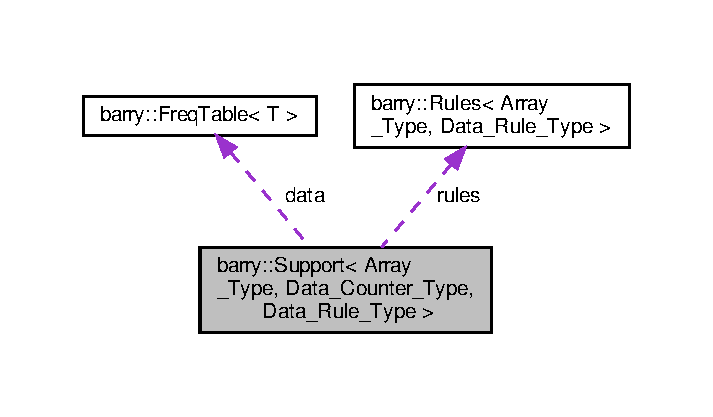
\includegraphics[width=190pt]{classbarry_1_1_support__coll__graph}
\end{center}
\end{figure}
\subsection*{Public Member Functions}
\begin{DoxyCompactItemize}
\item 
\hyperlink{classbarry_1_1_support_ab946f83af83c571de8bd5a17ce453240}{Support} (const Array\+\_\+\+Type $\ast$Array\+\_\+)
\item 
\hyperlink{classbarry_1_1_support_aa451bd21c09935b686869fef96c5b874}{Support} (\hyperlink{namespacebarry_a11dfc53ddb4672278319aa04f1e09a6c}{uint} N\+\_\+, \hyperlink{namespacebarry_a11dfc53ddb4672278319aa04f1e09a6c}{uint} M\+\_\+)
\item 
\hyperlink{classbarry_1_1_support_a1ffd5ee63fa68338cbbf443e1e54e5b4}{$\sim$\+Support} ()
\item 
void \hyperlink{classbarry_1_1_support_a5878ac60282fc1380c92f3ba502f249e}{reset} ()
\begin{DoxyCompactList}\small\item\em Resets the support calculator. \end{DoxyCompactList}\item 
void \hyperlink{classbarry_1_1_support_afbe207cc2762bc698c9ccb3212e9de78}{reset} (const Array\+\_\+\+Type $\ast$Array\+\_\+)
\item 
void \hyperlink{classbarry_1_1_support_a9fc89bd8b15dcad6a4140a3c74073d10}{add\+\_\+counter} (\hyperlink{classbarry_1_1_counter}{Counter}$<$ Array\+\_\+\+Type, Data\+\_\+\+Type $>$ \&f\+\_\+)
\item 
void \hyperlink{classbarry_1_1_support_ab5261952be0746f188ee024e3e8c26c1}{calc} (\hyperlink{namespacebarry_a11dfc53ddb4672278319aa04f1e09a6c}{uint} pos=0u, const bool \&diag=false, std\+::vector$<$ Array\+\_\+\+Type $>$ $\ast$array\+\_\+bank=nullptr, std\+::vector$<$ std\+::vector$<$ double $>$ $>$ $\ast$stats\+\_\+bank=nullptr)
\begin{DoxyCompactList}\small\item\em Computes the entire support. \end{DoxyCompactList}\end{DoxyCompactItemize}
\subsection*{Public Attributes}
\begin{DoxyCompactItemize}
\item 
const Array\+\_\+\+Type $\ast$ \hyperlink{classbarry_1_1_support_a782b1912d7fa2963d79d48a50947f033}{Array}
\item 
Data\+\_\+\+Type $\ast$ \hyperlink{classbarry_1_1_support_ad53c81c95b0a30ec2cea7e7e88774c0c}{data} = nullptr
\item 
Array\+\_\+\+Type \hyperlink{classbarry_1_1_support_ae26e46356041286028ffcc27195b9e8a}{Empty\+Array}
\item 
\hyperlink{classbarry_1_1_stats_d_b}{Stats\+DB} \hyperlink{classbarry_1_1_support_ac9942324040dfed9e0f2347b4d9d25b3}{support}
\item 
std\+::vector$<$ \hyperlink{classbarry_1_1_counter}{Counter}$<$ Array\+\_\+\+Type, Data\+\_\+\+Type $>$ $>$ \hyperlink{classbarry_1_1_support_a9615cb720931f81b57d5caa272b969ab}{counters}
\item 
std\+::vector$<$ double $>$ \hyperlink{classbarry_1_1_support_a094f0851c7d6bfa7876eb0df2be4439e}{current\+\_\+stats}
\item 
\hyperlink{namespacebarry_a11dfc53ddb4672278319aa04f1e09a6c}{uint} \hyperlink{classbarry_1_1_support_a1e3158ceae716505cb0c5fb14374be9b}{N}
\item 
\hyperlink{namespacebarry_a11dfc53ddb4672278319aa04f1e09a6c}{uint} \hyperlink{classbarry_1_1_support_aaceb2f83d235c70034e089087991cff8}{M}
\item 
bool \hyperlink{classbarry_1_1_support_a737bc10d6a6e4e3b18aeef0228bd45bb}{initialized} = false
\end{DoxyCompactItemize}


\subsection{Detailed Description}
\subsubsection*{template$<$typename Array\+\_\+\+Type = B\+Array$<$$>$, typename Data\+\_\+\+Type = bool$>$\newline
class barry\+::\+Support$<$ Array\+\_\+\+Type, Data\+\_\+\+Type $>$}

Compute the support of sufficient statistics. 

Given an array and a set of counters, this object iterates throughout the support set of the Array while at the same time computing the support of the sufficient statitics. 

Definition at line 18 of file barry.\+hpp.



\subsection{Constructor \& Destructor Documentation}
\mbox{\Hypertarget{classbarry_1_1_support_ab946f83af83c571de8bd5a17ce453240}\label{classbarry_1_1_support_ab946f83af83c571de8bd5a17ce453240}} 
\index{barry\+::\+Support@{barry\+::\+Support}!Support@{Support}}
\index{Support@{Support}!barry\+::\+Support@{barry\+::\+Support}}
\subsubsection{\texorpdfstring{Support()}{Support()}\hspace{0.1cm}{\footnotesize\ttfamily [1/2]}}
{\footnotesize\ttfamily template$<$typename Array\+\_\+\+Type  = B\+Array$<$$>$, typename Data\+\_\+\+Type  = bool$>$ \\
\hyperlink{classbarry_1_1_support}{barry\+::\+Support}$<$ Array\+\_\+\+Type, Data\+\_\+\+Type $>$\+::\hyperlink{classbarry_1_1_support}{Support} (\begin{DoxyParamCaption}\item[{const Array\+\_\+\+Type $\ast$}]{Array\+\_\+ }\end{DoxyParamCaption})\hspace{0.3cm}{\ttfamily [inline]}}



Definition at line 31 of file barry.\+hpp.

\mbox{\Hypertarget{classbarry_1_1_support_aa451bd21c09935b686869fef96c5b874}\label{classbarry_1_1_support_aa451bd21c09935b686869fef96c5b874}} 
\index{barry\+::\+Support@{barry\+::\+Support}!Support@{Support}}
\index{Support@{Support}!barry\+::\+Support@{barry\+::\+Support}}
\subsubsection{\texorpdfstring{Support()}{Support()}\hspace{0.1cm}{\footnotesize\ttfamily [2/2]}}
{\footnotesize\ttfamily template$<$typename Array\+\_\+\+Type  = B\+Array$<$$>$, typename Data\+\_\+\+Type  = bool$>$ \\
\hyperlink{classbarry_1_1_support}{barry\+::\+Support}$<$ Array\+\_\+\+Type, Data\+\_\+\+Type $>$\+::\hyperlink{classbarry_1_1_support}{Support} (\begin{DoxyParamCaption}\item[{\hyperlink{namespacebarry_a11dfc53ddb4672278319aa04f1e09a6c}{uint}}]{N\+\_\+,  }\item[{\hyperlink{namespacebarry_a11dfc53ddb4672278319aa04f1e09a6c}{uint}}]{M\+\_\+ }\end{DoxyParamCaption})\hspace{0.3cm}{\ttfamily [inline]}}



Definition at line 40 of file barry.\+hpp.

\mbox{\Hypertarget{classbarry_1_1_support_a1ffd5ee63fa68338cbbf443e1e54e5b4}\label{classbarry_1_1_support_a1ffd5ee63fa68338cbbf443e1e54e5b4}} 
\index{barry\+::\+Support@{barry\+::\+Support}!````~Support@{$\sim$\+Support}}
\index{````~Support@{$\sim$\+Support}!barry\+::\+Support@{barry\+::\+Support}}
\subsubsection{\texorpdfstring{$\sim$\+Support()}{~Support()}}
{\footnotesize\ttfamily template$<$typename Array\+\_\+\+Type  = B\+Array$<$$>$, typename Data\+\_\+\+Type  = bool$>$ \\
\hyperlink{classbarry_1_1_support}{barry\+::\+Support}$<$ Array\+\_\+\+Type, Data\+\_\+\+Type $>$\+::$\sim$\hyperlink{classbarry_1_1_support}{Support} (\begin{DoxyParamCaption}{ }\end{DoxyParamCaption})\hspace{0.3cm}{\ttfamily [inline]}}



Definition at line 41 of file barry.\+hpp.



\subsection{Member Function Documentation}
\mbox{\Hypertarget{classbarry_1_1_support_a9fc89bd8b15dcad6a4140a3c74073d10}\label{classbarry_1_1_support_a9fc89bd8b15dcad6a4140a3c74073d10}} 
\index{barry\+::\+Support@{barry\+::\+Support}!add\+\_\+counter@{add\+\_\+counter}}
\index{add\+\_\+counter@{add\+\_\+counter}!barry\+::\+Support@{barry\+::\+Support}}
\subsubsection{\texorpdfstring{add\+\_\+counter()}{add\_counter()}}
{\footnotesize\ttfamily template$<$typename Array\+\_\+\+Type , typename Data\+\_\+\+Type $>$ \\
void \hyperlink{classbarry_1_1_support}{Support}$<$ Array\+\_\+\+Type, Data\+\_\+\+Type $>$\+::add\+\_\+counter (\begin{DoxyParamCaption}\item[{\hyperlink{classbarry_1_1_counter}{Counter}$<$ Array\+\_\+\+Type, Data\+\_\+\+Type $>$ \&}]{f\+\_\+ }\end{DoxyParamCaption})\hspace{0.3cm}{\ttfamily [inline]}}



Definition at line 183 of file barry.\+hpp.

\mbox{\Hypertarget{classbarry_1_1_support_ab5261952be0746f188ee024e3e8c26c1}\label{classbarry_1_1_support_ab5261952be0746f188ee024e3e8c26c1}} 
\index{barry\+::\+Support@{barry\+::\+Support}!calc@{calc}}
\index{calc@{calc}!barry\+::\+Support@{barry\+::\+Support}}
\subsubsection{\texorpdfstring{calc()}{calc()}}
{\footnotesize\ttfamily template$<$typename Array\+\_\+\+Type , typename Data\+\_\+\+Type $>$ \\
void \hyperlink{classbarry_1_1_support}{Support}$<$ Array\+\_\+\+Type, Data\+\_\+\+Type $>$\+::calc (\begin{DoxyParamCaption}\item[{\hyperlink{namespacebarry_a11dfc53ddb4672278319aa04f1e09a6c}{uint}}]{pos = {\ttfamily 0u},  }\item[{const bool \&}]{diag = {\ttfamily false},  }\item[{std\+::vector$<$ Array\+\_\+\+Type $>$ $\ast$}]{array\+\_\+bank = {\ttfamily nullptr},  }\item[{std\+::vector$<$ std\+::vector$<$ double $>$ $>$ $\ast$}]{stats\+\_\+bank = {\ttfamily nullptr} }\end{DoxyParamCaption})\hspace{0.3cm}{\ttfamily [inline]}}



Computes the entire support. 

Not to be used by the user. Sets the starting point in the array (column-\/major).


\begin{DoxyParams}{Parameters}
{\em diag} & When {\ttfamily true}, includes the diagonal (i=j) in the counts.\\
\hline
{\em array\+\_\+bank} & If specified, the counter will add to the vector each possible state of the array, as it counts.\\
\hline
{\em stats\+\_\+bank} & If specified, the counter will add to the vector each possible set of statistics, as it counts. \\
\hline
\end{DoxyParams}


Definition at line 102 of file barry.\+hpp.

\mbox{\Hypertarget{classbarry_1_1_support_a5878ac60282fc1380c92f3ba502f249e}\label{classbarry_1_1_support_a5878ac60282fc1380c92f3ba502f249e}} 
\index{barry\+::\+Support@{barry\+::\+Support}!reset@{reset}}
\index{reset@{reset}!barry\+::\+Support@{barry\+::\+Support}}
\subsubsection{\texorpdfstring{reset()}{reset()}\hspace{0.1cm}{\footnotesize\ttfamily [1/2]}}
{\footnotesize\ttfamily template$<$typename Array\+\_\+\+Type , typename Data\+\_\+\+Type $>$ \\
void \hyperlink{classbarry_1_1_support}{Support}$<$ Array\+\_\+\+Type, Data\+\_\+\+Type $>$\+::reset (\begin{DoxyParamCaption}{ }\end{DoxyParamCaption})\hspace{0.3cm}{\ttfamily [inline]}}



Resets the support calculator. 

If needed, the counters of a support object can be reused.


\begin{DoxyParams}{Parameters}
{\em Array\+\_\+} & New array over which the support will be computed. \\
\hline
\end{DoxyParams}


Definition at line 79 of file barry.\+hpp.

\mbox{\Hypertarget{classbarry_1_1_support_afbe207cc2762bc698c9ccb3212e9de78}\label{classbarry_1_1_support_afbe207cc2762bc698c9ccb3212e9de78}} 
\index{barry\+::\+Support@{barry\+::\+Support}!reset@{reset}}
\index{reset@{reset}!barry\+::\+Support@{barry\+::\+Support}}
\subsubsection{\texorpdfstring{reset()}{reset()}\hspace{0.1cm}{\footnotesize\ttfamily [2/2]}}
{\footnotesize\ttfamily template$<$typename Array\+\_\+\+Type , typename Data\+\_\+\+Type $>$ \\
void \hyperlink{classbarry_1_1_support}{Support}$<$ Array\+\_\+\+Type, Data\+\_\+\+Type $>$\+::reset (\begin{DoxyParamCaption}\item[{const Array\+\_\+\+Type $\ast$}]{Array\+\_\+ }\end{DoxyParamCaption})\hspace{0.3cm}{\ttfamily [inline]}}



Definition at line 87 of file barry.\+hpp.



\subsection{Member Data Documentation}
\mbox{\Hypertarget{classbarry_1_1_support_a782b1912d7fa2963d79d48a50947f033}\label{classbarry_1_1_support_a782b1912d7fa2963d79d48a50947f033}} 
\index{barry\+::\+Support@{barry\+::\+Support}!Array@{Array}}
\index{Array@{Array}!barry\+::\+Support@{barry\+::\+Support}}
\subsubsection{\texorpdfstring{Array}{Array}}
{\footnotesize\ttfamily template$<$typename Array\+\_\+\+Type  = B\+Array$<$$>$, typename Data\+\_\+\+Type  = bool$>$ \\
const Array\+\_\+\+Type$\ast$ \hyperlink{classbarry_1_1_support}{barry\+::\+Support}$<$ Array\+\_\+\+Type, Data\+\_\+\+Type $>$\+::Array}



Definition at line 21 of file barry.\+hpp.

\mbox{\Hypertarget{classbarry_1_1_support_a9615cb720931f81b57d5caa272b969ab}\label{classbarry_1_1_support_a9615cb720931f81b57d5caa272b969ab}} 
\index{barry\+::\+Support@{barry\+::\+Support}!counters@{counters}}
\index{counters@{counters}!barry\+::\+Support@{barry\+::\+Support}}
\subsubsection{\texorpdfstring{counters}{counters}}
{\footnotesize\ttfamily template$<$typename Array\+\_\+\+Type  = B\+Array$<$$>$, typename Data\+\_\+\+Type  = bool$>$ \\
std\+::vector$<$ \hyperlink{classbarry_1_1_counter}{Counter}$<$Array\+\_\+\+Type, Data\+\_\+\+Type$>$ $>$ \hyperlink{classbarry_1_1_support}{barry\+::\+Support}$<$ Array\+\_\+\+Type, Data\+\_\+\+Type $>$\+::counters}



Definition at line 25 of file barry.\+hpp.

\mbox{\Hypertarget{classbarry_1_1_support_a094f0851c7d6bfa7876eb0df2be4439e}\label{classbarry_1_1_support_a094f0851c7d6bfa7876eb0df2be4439e}} 
\index{barry\+::\+Support@{barry\+::\+Support}!current\+\_\+stats@{current\+\_\+stats}}
\index{current\+\_\+stats@{current\+\_\+stats}!barry\+::\+Support@{barry\+::\+Support}}
\subsubsection{\texorpdfstring{current\+\_\+stats}{current\_stats}}
{\footnotesize\ttfamily template$<$typename Array\+\_\+\+Type  = B\+Array$<$$>$, typename Data\+\_\+\+Type  = bool$>$ \\
std\+::vector$<$ double $>$ \hyperlink{classbarry_1_1_support}{barry\+::\+Support}$<$ Array\+\_\+\+Type, Data\+\_\+\+Type $>$\+::current\+\_\+stats}



Definition at line 26 of file barry.\+hpp.

\mbox{\Hypertarget{classbarry_1_1_support_ad53c81c95b0a30ec2cea7e7e88774c0c}\label{classbarry_1_1_support_ad53c81c95b0a30ec2cea7e7e88774c0c}} 
\index{barry\+::\+Support@{barry\+::\+Support}!data@{data}}
\index{data@{data}!barry\+::\+Support@{barry\+::\+Support}}
\subsubsection{\texorpdfstring{data}{data}}
{\footnotesize\ttfamily template$<$typename Array\+\_\+\+Type  = B\+Array$<$$>$, typename Data\+\_\+\+Type  = bool$>$ \\
Data\+\_\+\+Type$\ast$ \hyperlink{classbarry_1_1_support}{barry\+::\+Support}$<$ Array\+\_\+\+Type, Data\+\_\+\+Type $>$\+::data = nullptr}



Definition at line 22 of file barry.\+hpp.

\mbox{\Hypertarget{classbarry_1_1_support_ae26e46356041286028ffcc27195b9e8a}\label{classbarry_1_1_support_ae26e46356041286028ffcc27195b9e8a}} 
\index{barry\+::\+Support@{barry\+::\+Support}!Empty\+Array@{Empty\+Array}}
\index{Empty\+Array@{Empty\+Array}!barry\+::\+Support@{barry\+::\+Support}}
\subsubsection{\texorpdfstring{Empty\+Array}{EmptyArray}}
{\footnotesize\ttfamily template$<$typename Array\+\_\+\+Type  = B\+Array$<$$>$, typename Data\+\_\+\+Type  = bool$>$ \\
Array\+\_\+\+Type \hyperlink{classbarry_1_1_support}{barry\+::\+Support}$<$ Array\+\_\+\+Type, Data\+\_\+\+Type $>$\+::Empty\+Array}



Definition at line 23 of file barry.\+hpp.

\mbox{\Hypertarget{classbarry_1_1_support_a737bc10d6a6e4e3b18aeef0228bd45bb}\label{classbarry_1_1_support_a737bc10d6a6e4e3b18aeef0228bd45bb}} 
\index{barry\+::\+Support@{barry\+::\+Support}!initialized@{initialized}}
\index{initialized@{initialized}!barry\+::\+Support@{barry\+::\+Support}}
\subsubsection{\texorpdfstring{initialized}{initialized}}
{\footnotesize\ttfamily template$<$typename Array\+\_\+\+Type  = B\+Array$<$$>$, typename Data\+\_\+\+Type  = bool$>$ \\
bool \hyperlink{classbarry_1_1_support}{barry\+::\+Support}$<$ Array\+\_\+\+Type, Data\+\_\+\+Type $>$\+::initialized = false}



Definition at line 29 of file barry.\+hpp.

\mbox{\Hypertarget{classbarry_1_1_support_aaceb2f83d235c70034e089087991cff8}\label{classbarry_1_1_support_aaceb2f83d235c70034e089087991cff8}} 
\index{barry\+::\+Support@{barry\+::\+Support}!M@{M}}
\index{M@{M}!barry\+::\+Support@{barry\+::\+Support}}
\subsubsection{\texorpdfstring{M}{M}}
{\footnotesize\ttfamily template$<$typename Array\+\_\+\+Type  = B\+Array$<$$>$, typename Data\+\_\+\+Type  = bool$>$ \\
\hyperlink{namespacebarry_a11dfc53ddb4672278319aa04f1e09a6c}{uint} \hyperlink{classbarry_1_1_support}{barry\+::\+Support}$<$ Array\+\_\+\+Type, Data\+\_\+\+Type $>$\+::M}



Definition at line 28 of file barry.\+hpp.

\mbox{\Hypertarget{classbarry_1_1_support_a1e3158ceae716505cb0c5fb14374be9b}\label{classbarry_1_1_support_a1e3158ceae716505cb0c5fb14374be9b}} 
\index{barry\+::\+Support@{barry\+::\+Support}!N@{N}}
\index{N@{N}!barry\+::\+Support@{barry\+::\+Support}}
\subsubsection{\texorpdfstring{N}{N}}
{\footnotesize\ttfamily template$<$typename Array\+\_\+\+Type  = B\+Array$<$$>$, typename Data\+\_\+\+Type  = bool$>$ \\
\hyperlink{namespacebarry_a11dfc53ddb4672278319aa04f1e09a6c}{uint} \hyperlink{classbarry_1_1_support}{barry\+::\+Support}$<$ Array\+\_\+\+Type, Data\+\_\+\+Type $>$\+::N}



Definition at line 28 of file barry.\+hpp.

\mbox{\Hypertarget{classbarry_1_1_support_ac9942324040dfed9e0f2347b4d9d25b3}\label{classbarry_1_1_support_ac9942324040dfed9e0f2347b4d9d25b3}} 
\index{barry\+::\+Support@{barry\+::\+Support}!support@{support}}
\index{support@{support}!barry\+::\+Support@{barry\+::\+Support}}
\subsubsection{\texorpdfstring{support}{support}}
{\footnotesize\ttfamily template$<$typename Array\+\_\+\+Type  = B\+Array$<$$>$, typename Data\+\_\+\+Type  = bool$>$ \\
\hyperlink{classbarry_1_1_stats_d_b}{Stats\+DB} \hyperlink{classbarry_1_1_support}{barry\+::\+Support}$<$ Array\+\_\+\+Type, Data\+\_\+\+Type $>$\+::support}



Definition at line 24 of file barry.\+hpp.



The documentation for this class was generated from the following file\+:\begin{DoxyCompactItemize}
\item 
include/\hyperlink{barry_8hpp}{barry.\+hpp}\end{DoxyCompactItemize}

\hypertarget{structbarry_1_1vec_hasher}{}\section{barry\+:\+:vec\+Hasher$<$ T $>$ Struct Template Reference}
\label{structbarry_1_1vec_hasher}\index{barry\+::vec\+Hasher$<$ T $>$@{barry\+::vec\+Hasher$<$ T $>$}}


{\ttfamily \#include $<$barry.\+hpp$>$}

\subsection*{Public Member Functions}
\begin{DoxyCompactItemize}
\item 
std\+::size\+\_\+t \hyperlink{structbarry_1_1vec_hasher_ada8dea483f4fc12f469e161b2fd09225}{operator()} (std\+::vector$<$ T $>$ const \&dat) const noexcept
\end{DoxyCompactItemize}


\subsection{Detailed Description}
\subsubsection*{template$<$typename T$>$\newline
struct barry\+::vec\+Hasher$<$ T $>$}



Definition at line 87 of file barry.\+hpp.



\subsection{Member Function Documentation}
\mbox{\Hypertarget{structbarry_1_1vec_hasher_ada8dea483f4fc12f469e161b2fd09225}\label{structbarry_1_1vec_hasher_ada8dea483f4fc12f469e161b2fd09225}} 
\index{barry\+::vec\+Hasher@{barry\+::vec\+Hasher}!operator()@{operator()}}
\index{operator()@{operator()}!barry\+::vec\+Hasher@{barry\+::vec\+Hasher}}
\subsubsection{\texorpdfstring{operator()()}{operator()()}}
{\footnotesize\ttfamily template$<$typename T $>$ \\
std\+::size\+\_\+t \hyperlink{structbarry_1_1vec_hasher}{barry\+::vec\+Hasher}$<$ T $>$\+::operator() (\begin{DoxyParamCaption}\item[{std\+::vector$<$ T $>$ const \&}]{dat }\end{DoxyParamCaption}) const\hspace{0.3cm}{\ttfamily [inline]}, {\ttfamily [noexcept]}}



Definition at line 88 of file barry.\+hpp.



The documentation for this struct was generated from the following file\+:\begin{DoxyCompactItemize}
\item 
include/barry/\hyperlink{barry_8hpp}{barry.\+hpp}\end{DoxyCompactItemize}

\hypertarget{structvec_hasher}{}\section{vec\+Hasher$<$ T $>$ Struct Template Reference}
\label{structvec_hasher}\index{vec\+Hasher$<$ T $>$@{vec\+Hasher$<$ T $>$}}


{\ttfamily \#include $<$statsdb.\+hpp$>$}

\subsection*{Public Member Functions}
\begin{DoxyCompactItemize}
\item 
std\+::size\+\_\+t \hyperlink{structvec_hasher_ae8127d9b7d302fe59bd64e7067e7ba61}{operator()} (std\+::vector$<$ T $>$ const \&dat) const noexcept
\end{DoxyCompactItemize}


\subsection{Detailed Description}
\subsubsection*{template$<$typename T$>$\newline
struct vec\+Hasher$<$ T $>$}



Definition at line 10 of file statsdb.\+hpp.



\subsection{Member Function Documentation}
\mbox{\Hypertarget{structvec_hasher_ae8127d9b7d302fe59bd64e7067e7ba61}\label{structvec_hasher_ae8127d9b7d302fe59bd64e7067e7ba61}} 
\index{vec\+Hasher@{vec\+Hasher}!operator()@{operator()}}
\index{operator()@{operator()}!vec\+Hasher@{vec\+Hasher}}
\subsubsection{\texorpdfstring{operator()()}{operator()()}}
{\footnotesize\ttfamily template$<$typename T $>$ \\
std\+::size\+\_\+t \hyperlink{structvec_hasher}{vec\+Hasher}$<$ T $>$\+::operator() (\begin{DoxyParamCaption}\item[{std\+::vector$<$ T $>$ const \&}]{dat }\end{DoxyParamCaption}) const\hspace{0.3cm}{\ttfamily [inline]}, {\ttfamily [noexcept]}}



Definition at line 11 of file statsdb.\+hpp.



The documentation for this struct was generated from the following file\+:\begin{DoxyCompactItemize}
\item 
include/\hyperlink{statsdb_8hpp}{statsdb.\+hpp}\end{DoxyCompactItemize}

\chapter{File Documentation}
\hypertarget{barray-bones_8hpp}{}\section{include/barray-\/bones.hpp File Reference}
\label{barray-bones_8hpp}\index{include/barray-\/bones.\+hpp@{include/barray-\/bones.\+hpp}}
{\ttfamily \#include \char`\"{}typedefs.\+hpp\char`\"{}}\newline
{\ttfamily \#include \char`\"{}cell-\/bones.\+hpp\char`\"{}}\newline
Include dependency graph for barray-\/bones.hpp\+:\nopagebreak
\begin{figure}[H]
\begin{center}
\leavevmode
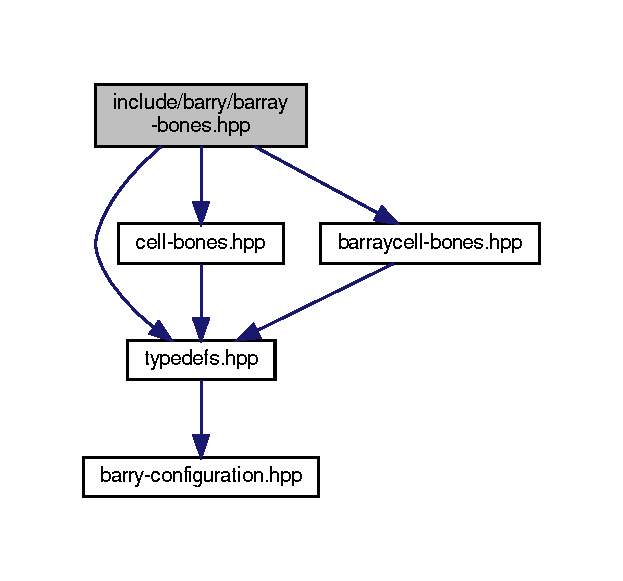
\includegraphics[width=217pt]{barray-bones_8hpp__incl}
\end{center}
\end{figure}
This graph shows which files directly or indirectly include this file\+:\nopagebreak
\begin{figure}[H]
\begin{center}
\leavevmode
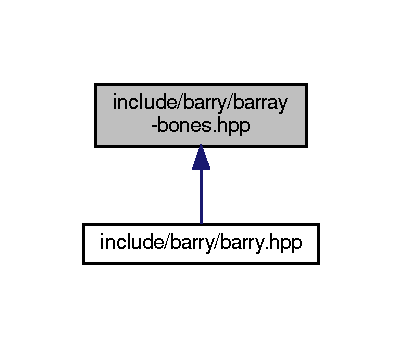
\includegraphics[width=350pt]{barray-bones_8hpp__dep__incl}
\end{center}
\end{figure}
\subsection*{Classes}
\begin{DoxyCompactItemize}
\item 
class \hyperlink{class_b_array}{B\+Array$<$ Cell\+\_\+\+Type, Data\+\_\+\+Type $>$}
\begin{DoxyCompactList}\small\item\em Baseline class for binary arrays. \end{DoxyCompactList}\end{DoxyCompactItemize}
\subsection*{Macros}
\begin{DoxyCompactItemize}
\item 
\#define \hyperlink{barray-bones_8hpp_a130b55fea4c46b3fc84dc76b641f5f0d}{B\+A\+R\+R\+A\+Y\+\_\+\+B\+O\+N\+E\+S\+\_\+\+H\+PP}~1
\end{DoxyCompactItemize}


\subsection{Macro Definition Documentation}
\mbox{\Hypertarget{barray-bones_8hpp_a130b55fea4c46b3fc84dc76b641f5f0d}\label{barray-bones_8hpp_a130b55fea4c46b3fc84dc76b641f5f0d}} 
\index{barray-\/bones.\+hpp@{barray-\/bones.\+hpp}!B\+A\+R\+R\+A\+Y\+\_\+\+B\+O\+N\+E\+S\+\_\+\+H\+PP@{B\+A\+R\+R\+A\+Y\+\_\+\+B\+O\+N\+E\+S\+\_\+\+H\+PP}}
\index{B\+A\+R\+R\+A\+Y\+\_\+\+B\+O\+N\+E\+S\+\_\+\+H\+PP@{B\+A\+R\+R\+A\+Y\+\_\+\+B\+O\+N\+E\+S\+\_\+\+H\+PP}!barray-\/bones.\+hpp@{barray-\/bones.\+hpp}}
\subsubsection{\texorpdfstring{B\+A\+R\+R\+A\+Y\+\_\+\+B\+O\+N\+E\+S\+\_\+\+H\+PP}{BARRAY\_BONES\_HPP}}
{\footnotesize\ttfamily \#define B\+A\+R\+R\+A\+Y\+\_\+\+B\+O\+N\+E\+S\+\_\+\+H\+PP~1}



Definition at line 7 of file barray-\/bones.\+hpp.


\hypertarget{barray-iterator_8hpp}{}\section{include/barray-\/iterator.hpp File Reference}
\label{barray-iterator_8hpp}\index{include/barray-\/iterator.\+hpp@{include/barray-\/iterator.\+hpp}}
{\ttfamily \#include \char`\"{}typedefs.\+hpp\char`\"{}}\newline
{\ttfamily \#include \char`\"{}barray-\/bones.\+hpp\char`\"{}}\newline
Include dependency graph for barray-\/iterator.hpp\+:
\nopagebreak
\begin{figure}[H]
\begin{center}
\leavevmode
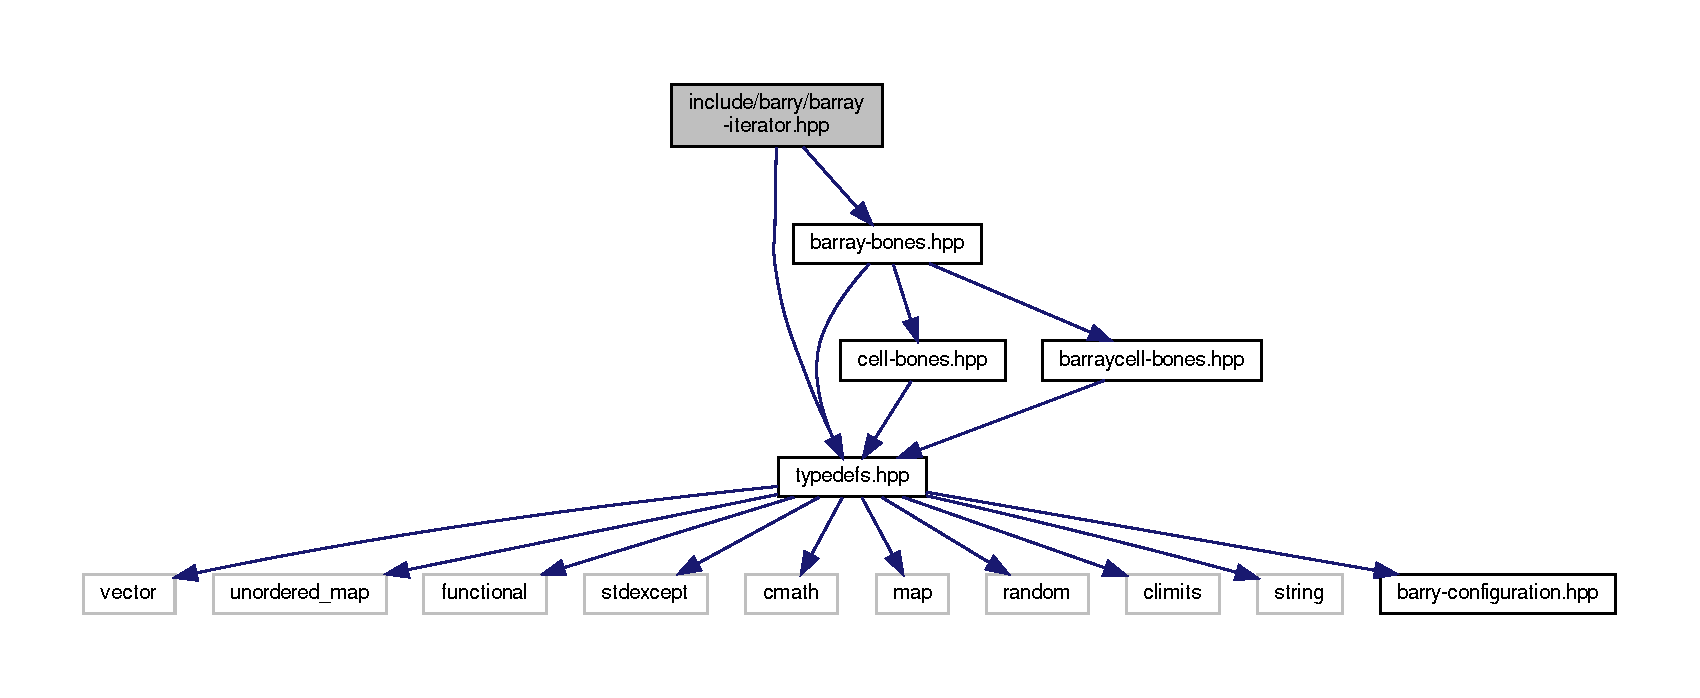
\includegraphics[width=350pt]{barray-iterator_8hpp__incl}
\end{center}
\end{figure}
\subsection*{Classes}
\begin{DoxyCompactItemize}
\item 
class \hyperlink{class_const_b_array_row_iter}{Const\+B\+Array\+Row\+Iter$<$ Cell\+\_\+\+Type, Data\+\_\+\+Type $>$}
\end{DoxyCompactItemize}
\subsection*{Macros}
\begin{DoxyCompactItemize}
\item 
\#define \hyperlink{barray-iterator_8hpp_af7d28058e98dd1797def3cd230abe121}{B\+A\+R\+R\+A\+Y\+\_\+\+I\+T\+E\+R\+A\+T\+O\+R\+\_\+\+H\+PP}~1
\end{DoxyCompactItemize}


\subsection{Macro Definition Documentation}
\mbox{\Hypertarget{barray-iterator_8hpp_af7d28058e98dd1797def3cd230abe121}\label{barray-iterator_8hpp_af7d28058e98dd1797def3cd230abe121}} 
\index{barray-\/iterator.\+hpp@{barray-\/iterator.\+hpp}!B\+A\+R\+R\+A\+Y\+\_\+\+I\+T\+E\+R\+A\+T\+O\+R\+\_\+\+H\+PP@{B\+A\+R\+R\+A\+Y\+\_\+\+I\+T\+E\+R\+A\+T\+O\+R\+\_\+\+H\+PP}}
\index{B\+A\+R\+R\+A\+Y\+\_\+\+I\+T\+E\+R\+A\+T\+O\+R\+\_\+\+H\+PP@{B\+A\+R\+R\+A\+Y\+\_\+\+I\+T\+E\+R\+A\+T\+O\+R\+\_\+\+H\+PP}!barray-\/iterator.\+hpp@{barray-\/iterator.\+hpp}}
\subsubsection{\texorpdfstring{B\+A\+R\+R\+A\+Y\+\_\+\+I\+T\+E\+R\+A\+T\+O\+R\+\_\+\+H\+PP}{BARRAY\_ITERATOR\_HPP}}
{\footnotesize\ttfamily \#define B\+A\+R\+R\+A\+Y\+\_\+\+I\+T\+E\+R\+A\+T\+O\+R\+\_\+\+H\+PP~1}



Definition at line 7 of file barray-\/iterator.\+hpp.


\hypertarget{barray-meat_8hpp}{}\doxysection{include/barry/barray-\/meat.hpp File Reference}
\label{barray-meat_8hpp}\index{include/barry/barray-\/meat.hpp@{include/barry/barray-\/meat.hpp}}
{\ttfamily \#include \char`\"{}barray-\/bones.\+hpp\char`\"{}}\newline
Include dependency graph for barray-\/meat.hpp\+:
\nopagebreak
\begin{figure}[H]
\begin{center}
\leavevmode
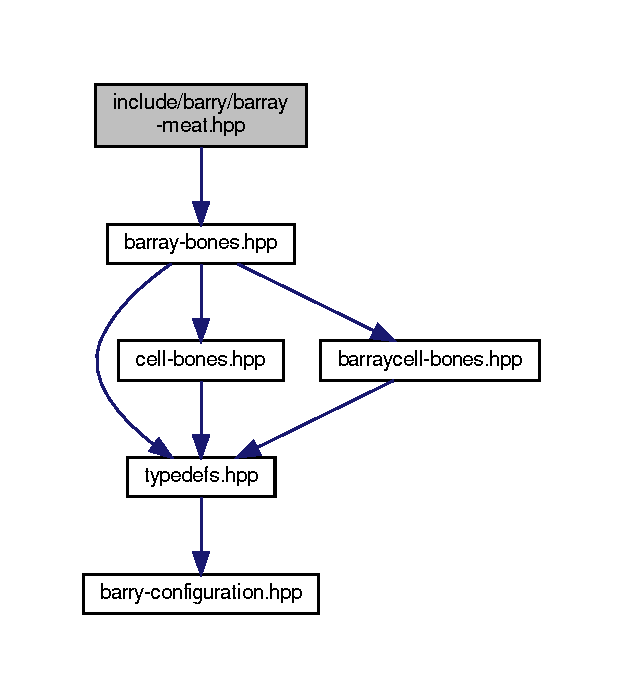
\includegraphics[width=350pt]{barray-meat_8hpp__incl}
\end{center}
\end{figure}
This graph shows which files directly or indirectly include this file\+:
\nopagebreak
\begin{figure}[H]
\begin{center}
\leavevmode
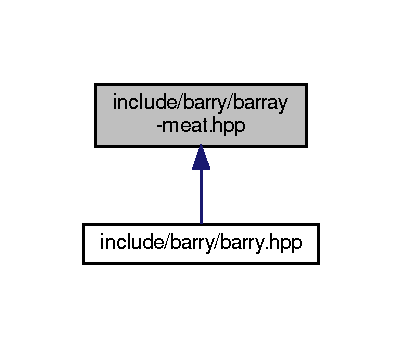
\includegraphics[width=193pt]{barray-meat_8hpp__dep__incl}
\end{center}
\end{figure}
\doxysubsection*{Macros}
\begin{DoxyCompactItemize}
\item 
\#define \mbox{\hyperlink{barray-meat_8hpp_ac63c3ae8d3d35d7ac99e5d4568703cc0}{BARRAY\+\_\+\+TYPE}}()~\mbox{\hyperlink{class_b_array}{BArray}}$<$Cell\+\_\+\+Type, Data\+\_\+\+Type$>$
\item 
\#define \mbox{\hyperlink{barray-meat_8hpp_a5b8ac6aa8527ed4e649879db889d033b}{BARRAY\+\_\+\+TEMPLATE\+\_\+\+ARGS}}()~$<$typename Cell\+\_\+\+Type, typename Data\+\_\+\+Type$>$
\item 
\#define \mbox{\hyperlink{barray-meat_8hpp_af13a653838bf7594b0fb9f15f8a49218}{BARRAY\+\_\+\+TEMPLATE}}(a,  b)~    template \mbox{\hyperlink{barray-meat-operators_8hpp_a6bc423fbf0bf597cd9f254334d29fa0b}{BARRAY\+\_\+\+TEMPLATE\+\_\+\+ARGS}}() inline a \mbox{\hyperlink{barray-meat-operators_8hpp_aa088d077e347efbf290ceeed03ca0d22}{BARRAY\+\_\+\+TYPE}}()\+::b
\item 
\#define \mbox{\hyperlink{barray-meat_8hpp_a391c25765afb3eb7b8288b21dd2eb16b}{ROW}}(a)~\mbox{\hyperlink{counters-meat_8hpp_a2dd4d78a0686fa444ac77760d7446ca3}{this}}-\/$>$el\+\_\+ij\mbox{[}a\mbox{]}
\item 
\#define \mbox{\hyperlink{barray-meat_8hpp_ac2a0f8cf6ac7fdad243406f6e3ea0605}{COL}}(a)~\mbox{\hyperlink{counters-meat_8hpp_a2dd4d78a0686fa444ac77760d7446ca3}{this}}-\/$>$el\+\_\+ji\mbox{[}a\mbox{]}
\end{DoxyCompactItemize}
\doxysubsection*{Functions}
\begin{DoxyCompactItemize}
\item 
\mbox{\hyperlink{barray-meat_8hpp_ab379b1e66687ab09c9bf7c9f384c615b}{BARRAY\+\_\+\+TEMPLATE}} (, \mbox{\hyperlink{class_b_array}{BArray}})(\mbox{\hyperlink{typedefs_8hpp_a91ad9478d81a7aaf2593e8d9c3d06a14}{uint}} N\+\_\+
\item 
el\+\_\+ij \mbox{\hyperlink{barray-meat_8hpp_ae7864209a16418b52c060e3df05cfb1d}{resize}} (\mbox{\hyperlink{barraydense-meat_8hpp_a8cc2e7240164328fdc3f0e5e21032c56}{N}})
\item 
el\+\_\+ji \mbox{\hyperlink{barray-meat_8hpp_ab86136f19f6ddead546b015bf04dc112}{resize}} (\mbox{\hyperlink{barraydense-meat_8hpp_adb61ad66dabc2db1f586c93e095ef9d3}{M}})
\item 
\mbox{\hyperlink{barray-meat_8hpp_a8b04c8536edde866596e149f2596e451}{for}} (\mbox{\hyperlink{typedefs_8hpp_a91ad9478d81a7aaf2593e8d9c3d06a14}{uint}} \mbox{\hyperlink{counters-meat_8hpp_aa0ecde9bec2f4c6686780ccf4f5fe835}{i}}=0u;\mbox{\hyperlink{counters-meat_8hpp_aa0ecde9bec2f4c6686780ccf4f5fe835}{i}}$<$ source.\+size();++\mbox{\hyperlink{counters-meat_8hpp_aa0ecde9bec2f4c6686780ccf4f5fe835}{i}})
\item 
Data\+\_\+\+Type bool \mbox{\hyperlink{barray-meat_8hpp_a96d6e901dc162f711d087a519d039923}{M}} (Array\+\_\+.\+M)
\item 
\mbox{\hyperlink{barray-meat_8hpp_a05fb0e53255f9fbca20d6cb2681fc58a}{BARRAY\+\_\+\+TEMPLATE}} (\mbox{\hyperlink{barray-meat-operators_8hpp_aa088d077e347efbf290ceeed03ca0d22}{BARRAY\+\_\+\+TYPE}}() \&, operator=)(\mbox{\hyperlink{barraydense-meat_8hpp_a92b303b76a3f942ea819498907d5e83c}{const}} \mbox{\hyperlink{class_b_array}{BArray}}$<$ Cell\+\_\+\+Type
\item 
\mbox{\hyperlink{barray-meat_8hpp_abc340348bce10b147bc07f1367e14f4e}{BARRAY\+\_\+\+TEMPLATE}} (, \mbox{\hyperlink{class_b_array}{BArray}})(\mbox{\hyperlink{barray-meat-operators_8hpp_aa088d077e347efbf290ceeed03ca0d22}{BARRAY\+\_\+\+TYPE}}() \&\&x) \mbox{\hyperlink{counters-meat_8hpp_ae763aeff9df78ca7be5f904fa4bbdc09}{noexcept}}
\item 
\mbox{\hyperlink{barray-meat_8hpp_a865f2b939b6482b835c88ef9280148f6}{BARRAY\+\_\+\+TEMPLATE}} (\mbox{\hyperlink{barray-meat-operators_8hpp_aa088d077e347efbf290ceeed03ca0d22}{BARRAY\+\_\+\+TYPE}}() \&, operator=)(\mbox{\hyperlink{barray-meat-operators_8hpp_aa088d077e347efbf290ceeed03ca0d22}{BARRAY\+\_\+\+TYPE}}() \&\&x) \mbox{\hyperlink{counters-meat_8hpp_ae763aeff9df78ca7be5f904fa4bbdc09}{noexcept}}
\item 
\mbox{\hyperlink{barray-meat_8hpp_ad316c2b2c73f532ba7eead8e821367ab}{BARRAY\+\_\+\+TEMPLATE}} (bool, operator==)(\mbox{\hyperlink{barraydense-meat_8hpp_a92b303b76a3f942ea819498907d5e83c}{const}} \mbox{\hyperlink{barray-meat-operators_8hpp_aa088d077e347efbf290ceeed03ca0d22}{BARRAY\+\_\+\+TYPE}}() \&\mbox{\hyperlink{barray-meat_8hpp_a6cb31aaad809d508e214b61785d7fb47}{Array\+\_\+}})
\item 
\mbox{\hyperlink{barray-meat_8hpp_ae9962ae7bb26fa819a29eabc482eb607}{BARRAY\+\_\+\+TEMPLATE}} (,$\sim$\mbox{\hyperlink{class_b_array}{BArray}})()
\item 
\mbox{\hyperlink{barray-meat_8hpp_a206392f061f5ce6eeba276a24266488a}{BARRAY\+\_\+\+TEMPLATE}} (void, set\+\_\+data)(Data\+\_\+\+Type $\ast$\mbox{\hyperlink{counters-meat_8hpp_afb5ad8f08fd716bba9cf4c1760f11927}{data\+\_\+}}
\item 
\mbox{\hyperlink{barray-meat_8hpp_adc7a47e0ebd230fbfbc406d755f104d9}{BARRAY\+\_\+\+TEMPLATE}} (Data\+\_\+\+Type $\ast$, D)()
\item 
\mbox{\hyperlink{barray-meat_8hpp_ad52c7e64a12826aee19213c8d2e5cb16}{BARRAY\+\_\+\+TEMPLATE}} (void, out\+\_\+of\+\_\+range)(\mbox{\hyperlink{typedefs_8hpp_a91ad9478d81a7aaf2593e8d9c3d06a14}{uint}} \mbox{\hyperlink{counters-meat_8hpp_aa0ecde9bec2f4c6686780ccf4f5fe835}{i}}
\item 
\mbox{\hyperlink{barray-meat_8hpp_a8493026b6fc68d741665f31b755fce60}{BARRAY\+\_\+\+TEMPLATE}} (Cell\+\_\+\+Type, get\+\_\+cell)(\mbox{\hyperlink{typedefs_8hpp_a91ad9478d81a7aaf2593e8d9c3d06a14}{uint}} \mbox{\hyperlink{counters-meat_8hpp_aa0ecde9bec2f4c6686780ccf4f5fe835}{i}}
\item 
\mbox{\hyperlink{barray-meat_8hpp_a7392988f028c03d9e341d75a47403068}{if}} (\mbox{\hyperlink{barray-meat_8hpp_adebf5af9ec07cd7e67e2dcf776d6230b}{ROW}}(\mbox{\hyperlink{counters-meat_8hpp_aa0ecde9bec2f4c6686780ccf4f5fe835}{i}}).size()==0u) \mbox{\hyperlink{barray-meat_8hpp_a4725aca18f0b3220c56baad1a1ffc023}{return}}(Cell\+\_\+\+Type) 0.\+0
\item 
\mbox{\hyperlink{barray-meat_8hpp_a473282f8c2b44cf2bb49a8893bb35d2b}{if}} (\mbox{\hyperlink{barray-meat_8hpp_a35e7b789344a67f5d492ebd1c05e261d}{search}} !=\mbox{\hyperlink{barray-meat_8hpp_adebf5af9ec07cd7e67e2dcf776d6230b}{ROW}}(\mbox{\hyperlink{counters-meat_8hpp_aa0ecde9bec2f4c6686780ccf4f5fe835}{i}}).end()) \mbox{\hyperlink{barray-meat_8hpp_a4725aca18f0b3220c56baad1a1ffc023}{return}} \mbox{\hyperlink{barray-meat_8hpp_a35e7b789344a67f5d492ebd1c05e261d}{search}} -\/$>$ \mbox{\hyperlink{barraydense-meat_8hpp_a7c51d076c92c9801c8129c4214b7bcec}{second.\+value}}
\item 
\mbox{\hyperlink{barray-meat_8hpp_a4725aca18f0b3220c56baad1a1ffc023}{return}} (Cell\+\_\+\+Type) 0.\+0
\item 
\mbox{\hyperlink{barray-meat_8hpp_a6e1e09801521041a92dbea338b502c8c}{BARRAY\+\_\+\+TEMPLATE}} (std\+::vector$<$ Cell\+\_\+\+Type $>$, get\+\_\+row\+\_\+vec)(\mbox{\hyperlink{typedefs_8hpp_a91ad9478d81a7aaf2593e8d9c3d06a14}{uint}} \mbox{\hyperlink{counters-meat_8hpp_aa0ecde9bec2f4c6686780ccf4f5fe835}{i}}
\item 
std\+::vector$<$ Cell\+\_\+\+Type $>$ \mbox{\hyperlink{barray-meat_8hpp_a12eee12d7ad4ae646f30b21cd540cc2e}{ans}} (ncol(),(Cell\+\_\+\+Type) \mbox{\hyperlink{barraydense-meat_8hpp_ae6c865df784842196d411c1466b01686}{false}})
\item 
\mbox{\hyperlink{barray-meat_8hpp_ae8aac1f0ca098820ff4c54f7b3566218}{for}} (\mbox{\hyperlink{barraydense-meat_8hpp_a92b303b76a3f942ea819498907d5e83c}{const}} auto \&iter \+:row(\mbox{\hyperlink{counters-meat_8hpp_aa0ecde9bec2f4c6686780ccf4f5fe835}{i}}, \mbox{\hyperlink{barraydense-meat_8hpp_ae6c865df784842196d411c1466b01686}{false}})) \mbox{\hyperlink{barraydense-meat_8hpp_a2e094024a44e50938f0b8faecb5a82d8}{ans}}\mbox{[}\mbox{\hyperlink{barray-meat_8hpp_a2ec77210c1e75f63aada9cde5c937ceb}{iter.\+first}}\mbox{]}
\item 
\mbox{\hyperlink{barray-meat_8hpp_a3b4fca1016c80c61897a8cedaaa08d4d}{BARRAY\+\_\+\+TEMPLATE}} (void, get\+\_\+row\+\_\+vec)(std
\item 
\mbox{\hyperlink{barray-meat_8hpp_a65ba7c41e4057c0d6e9f76b8a0511eed}{BARRAY\+\_\+\+TEMPLATE}} (\mbox{\hyperlink{barray-meat-operators_8hpp_aa088d077e347efbf290ceeed03ca0d22}{BARRAY\+\_\+\+TYPE}}() \&, operator-\/=)(\mbox{\hyperlink{barraydense-meat_8hpp_a92b303b76a3f942ea819498907d5e83c}{const}} std
\item 
\mbox{\hyperlink{barray-meat_8hpp_aeede4027693fa19366fa9e7e194332dd}{BARRAY\+\_\+\+TEMPLATE}} (void, \mbox{\hyperlink{support-meat_8hpp_ab532d2e43799a4eda296996fae57a22f}{insert\+\_\+cell}})(\mbox{\hyperlink{typedefs_8hpp_a91ad9478d81a7aaf2593e8d9c3d06a14}{uint}} \mbox{\hyperlink{counters-meat_8hpp_aa0ecde9bec2f4c6686780ccf4f5fe835}{i}}
\item 
\mbox{\hyperlink{barray-meat_8hpp_a9545e9e49f9298a26c585e557b52413d}{if}} (\mbox{\hyperlink{barraydense-meat_8hpp_a55f9b5f5029c8d5cb64a0c3f2a86b41c}{check\+\_\+exists}})
\item 
\mbox{\hyperlink{barray-meat_8hpp_a9b8c44edae0485e461f86ff37b430d0b}{COL}} (\mbox{\hyperlink{statscounter-meat_8hpp_abbe66f29402555d707260862a10eb56e}{j}}).emplace(\mbox{\hyperlink{counters-meat_8hpp_aa0ecde9bec2f4c6686780ccf4f5fe835}{i}}
\item 
\& \mbox{\hyperlink{barray-meat_8hpp_ab0ecf56654c1482f9ba5df87b3afa180}{ROW}} (\mbox{\hyperlink{counters-meat_8hpp_aa0ecde9bec2f4c6686780ccf4f5fe835}{i}})\mbox{[}\mbox{\hyperlink{statscounter-meat_8hpp_abbe66f29402555d707260862a10eb56e}{j}}\mbox{]})
\item 
\mbox{\hyperlink{barray-meat_8hpp_a88e40ae786e7394af8d9c4d7f4dcdfb5}{BARRAY\+\_\+\+TEMPLATE}} (void, swap\+\_\+cells)(\mbox{\hyperlink{typedefs_8hpp_a91ad9478d81a7aaf2593e8d9c3d06a14}{uint}} i0
\item 
\mbox{\hyperlink{barray-meat_8hpp_acb65203198239b3f540b6e6f8c9efcbe}{if}} (\mbox{\hyperlink{barraydense-meat_8hpp_a1c97d677615ab6c6430f1a5908d3d248}{report}} !=nullptr)($\ast$\mbox{\hyperlink{barraydense-meat_8hpp_a1c97d677615ab6c6430f1a5908d3d248}{report}})
\item 
\mbox{\hyperlink{barray-meat_8hpp_a11a43692b8a84c51fb1c1947040d55f4}{if}} (check0 \&check1)
\item 
\mbox{\hyperlink{support-meat_8hpp_a0544c3fe466e421738dae463968b70ba}{else}} \mbox{\hyperlink{barray-meat_8hpp_ab3e92e830c19645e08147d844814ed15}{if}} (!check0 \&check1)
\item 
\mbox{\hyperlink{support-meat_8hpp_a0544c3fe466e421738dae463968b70ba}{else}} \mbox{\hyperlink{barray-meat_8hpp_a83a48ee41a450e99464538005b262934}{if}} (check0 \&!check1)
\item 
\mbox{\hyperlink{barray-meat_8hpp_a069ccf02f1040dd1b7aa13a33617d27e}{BARRAY\+\_\+\+TEMPLATE}} (void, toggle\+\_\+cell)(\mbox{\hyperlink{typedefs_8hpp_a91ad9478d81a7aaf2593e8d9c3d06a14}{uint}} \mbox{\hyperlink{counters-meat_8hpp_aa0ecde9bec2f4c6686780ccf4f5fe835}{i}}
\item 
\mbox{\hyperlink{barray-meat_8hpp_ad0abf78522405df2ce13d81f4e08ec81}{BARRAY\+\_\+\+TEMPLATE}} (void, swap\+\_\+rows)(\mbox{\hyperlink{typedefs_8hpp_a91ad9478d81a7aaf2593e8d9c3d06a14}{uint}} i0
\item 
\mbox{\hyperlink{barray-meat_8hpp_a9c458194455cb842393bbbc9e4196579}{if}} (\mbox{\hyperlink{barray-meat_8hpp_adebf5af9ec07cd7e67e2dcf776d6230b}{ROW}}(i0).size()==0u) move0
\item 
\mbox{\hyperlink{barray-meat_8hpp_af1a69de3f8efdce61192a3813845f28a}{if}} (\mbox{\hyperlink{barray-meat_8hpp_adebf5af9ec07cd7e67e2dcf776d6230b}{ROW}}(\mbox{\hyperlink{barraydense-meat_8hpp_ae53ac559c37574f7895e8af57d87f849}{i1}}).size()==0u) move1
\item 
\mbox{\hyperlink{barray-meat_8hpp_a0839ee74b40539432425dcf2bc0bbf91}{if}} (!move0 \&\&!move1) \mbox{\hyperlink{barray-meat_8hpp_a4725aca18f0b3220c56baad1a1ffc023}{return}}
\item 
\mbox{\hyperlink{barray-meat_8hpp_adebf5af9ec07cd7e67e2dcf776d6230b}{ROW}} (i0).swap(ROW(\mbox{\hyperlink{barraydense-meat_8hpp_ae53ac559c37574f7895e8af57d87f849}{i1}}))
\item 
\mbox{\hyperlink{barray-meat_8hpp_aeeb31868f975eeb570215f31ae928be1}{BARRAY\+\_\+\+TEMPLATE}} (void, swap\+\_\+cols)(\mbox{\hyperlink{typedefs_8hpp_a91ad9478d81a7aaf2593e8d9c3d06a14}{uint}} \mbox{\hyperlink{barraydense-meat_8hpp_a76215ac0aab4542631c11206d92597e2}{j0}}
\item 
\mbox{\hyperlink{barray-meat_8hpp_af3f7115c83f47f2d6f61dff2a62dc939}{if}} (\mbox{\hyperlink{barray-meat_8hpp_a9b8c44edae0485e461f86ff37b430d0b}{COL}}(\mbox{\hyperlink{barraydense-meat_8hpp_a76215ac0aab4542631c11206d92597e2}{j0}}).size()==0u) check0
\item 
\mbox{\hyperlink{barray-meat_8hpp_ae07e7cc10229100eda78de5b8c5f07ce}{if}} (\mbox{\hyperlink{barray-meat_8hpp_a9b8c44edae0485e461f86ff37b430d0b}{COL}}(\mbox{\hyperlink{barraydense-meat_8hpp_a355f2dae482006084fd82d31f52cbbc1}{j1}}).size()==0u) check1
\item 
\mbox{\hyperlink{barray-meat_8hpp_af5515b6c59b1c043d59299929f5389c3}{if}} (check0 \&\&check1)
\item 
\mbox{\hyperlink{support-meat_8hpp_a0544c3fe466e421738dae463968b70ba}{else}} \mbox{\hyperlink{barray-meat_8hpp_ae2397fb65cfb0df3e91daba11f523325}{if}} (check0 \&\&!check1)
\item 
\mbox{\hyperlink{support-meat_8hpp_a0544c3fe466e421738dae463968b70ba}{else}} \mbox{\hyperlink{barray-meat_8hpp_a2670b7febaa1b1f0157d5a3c997b6bd5}{if}} (!check0 \&\&check1)
\item 
\mbox{\hyperlink{barray-meat_8hpp_aa39f872b06a5776a3a07f054dd9b34b1}{BARRAY\+\_\+\+TEMPLATE}} (void, zero\+\_\+row)(\mbox{\hyperlink{typedefs_8hpp_a91ad9478d81a7aaf2593e8d9c3d06a14}{uint}} \mbox{\hyperlink{counters-meat_8hpp_aa0ecde9bec2f4c6686780ccf4f5fe835}{i}}
\item 
\mbox{\hyperlink{barray-meat_8hpp_a009384dc163a2dc0f6d5465933ef3aa2}{for}} (auto row=row0.\+begin();row !=row0.\+end();++row) \mbox{\hyperlink{support-meat_8hpp_a374b4083f6045b49bcde35a8da4d5e80}{rm\+\_\+cell}}(\mbox{\hyperlink{counters-meat_8hpp_aa0ecde9bec2f4c6686780ccf4f5fe835}{i}}
\item 
\mbox{\hyperlink{barray-meat_8hpp_a071acdda91bf05cde66638e57e6a8ddb}{BARRAY\+\_\+\+TEMPLATE}} (void, zero\+\_\+col)(\mbox{\hyperlink{typedefs_8hpp_a91ad9478d81a7aaf2593e8d9c3d06a14}{uint}} \mbox{\hyperlink{statscounter-meat_8hpp_abbe66f29402555d707260862a10eb56e}{j}}
\item 
\mbox{\hyperlink{barray-meat_8hpp_acf13f0d140cfe4bba66b40e934ab7904}{if}} (\mbox{\hyperlink{barray-meat_8hpp_a9b8c44edae0485e461f86ff37b430d0b}{COL}}(\mbox{\hyperlink{statscounter-meat_8hpp_abbe66f29402555d707260862a10eb56e}{j}}).size()==0u) \mbox{\hyperlink{barray-meat_8hpp_a4725aca18f0b3220c56baad1a1ffc023}{return}}
\item 
\mbox{\hyperlink{barray-meat_8hpp_a92e904728ae60a0c28c17516418e34f5}{BARRAY\+\_\+\+TEMPLATE}} (void, transpose)()
\item 
\mbox{\hyperlink{barray-meat_8hpp_a468d91a5cb53142e5d7fb17e8d94afd2}{BARRAY\+\_\+\+TEMPLATE}} (void, \mbox{\hyperlink{statscounter-meat_8hpp_acdeee95221bfcd8b7b9e1c2e1776259c}{clear}})(bool hard)
\item 
\mbox{\hyperlink{barray-meat_8hpp_a2289d926f0d0d7c5236791c6efea899a}{BARRAY\+\_\+\+TEMPLATE}} (void, \mbox{\hyperlink{statscounter-meat_8hpp_ae40d2e4f8ecd8bbe53d42f61bc802f8d}{resize}})(\mbox{\hyperlink{typedefs_8hpp_a91ad9478d81a7aaf2593e8d9c3d06a14}{uint}} N\+\_\+
\item 
\mbox{\hyperlink{barray-meat_8hpp_a8ed77e31dc7fd2d06507674739bd8f4a}{if}} (\mbox{\hyperlink{barraydense-meat_8hpp_a7ba174ad6ce79b3f56bf6d0ce0d93e34}{M\+\_\+}}$<$ \mbox{\hyperlink{barraydense-meat_8hpp_adb61ad66dabc2db1f586c93e095ef9d3}{M}}) \mbox{\hyperlink{support-meat_8hpp_a60708372bc78ab014d166f99ad509b41}{for}}(\mbox{\hyperlink{typedefs_8hpp_a91ad9478d81a7aaf2593e8d9c3d06a14}{uint}} \mbox{\hyperlink{statscounter-meat_8hpp_abbe66f29402555d707260862a10eb56e}{j}} = N\+\_\+
\end{DoxyCompactItemize}
\doxysubsection*{Variables}
\begin{DoxyCompactItemize}
\item 
\mbox{\hyperlink{typedefs_8hpp_a91ad9478d81a7aaf2593e8d9c3d06a14}{uint}} \mbox{\hyperlink{barray-meat_8hpp_a7ba174ad6ce79b3f56bf6d0ce0d93e34}{M\+\_\+}}
\item 
\mbox{\hyperlink{typedefs_8hpp_a91ad9478d81a7aaf2593e8d9c3d06a14}{uint}} \mbox{\hyperlink{barraydense-meat_8hpp_a92b303b76a3f942ea819498907d5e83c}{const}} std\+::vector$<$ \mbox{\hyperlink{typedefs_8hpp_a91ad9478d81a7aaf2593e8d9c3d06a14}{uint}} $>$ \& \mbox{\hyperlink{barray-meat_8hpp_ab3aa82e361912925fc1ecaf85e5041bf}{source}}
\item 
\mbox{\hyperlink{typedefs_8hpp_a91ad9478d81a7aaf2593e8d9c3d06a14}{uint}} \mbox{\hyperlink{barraydense-meat_8hpp_a92b303b76a3f942ea819498907d5e83c}{const}} std\+::vector$<$ \mbox{\hyperlink{typedefs_8hpp_a91ad9478d81a7aaf2593e8d9c3d06a14}{uint}} $>$ \mbox{\hyperlink{barraydense-meat_8hpp_a92b303b76a3f942ea819498907d5e83c}{const}} std\+::vector$<$ \mbox{\hyperlink{typedefs_8hpp_a91ad9478d81a7aaf2593e8d9c3d06a14}{uint}} $>$ \& \mbox{\hyperlink{barray-meat_8hpp_a653ae33b3514ffbd1ba2223a9e23764b}{target}}
\item 
\mbox{\hyperlink{typedefs_8hpp_a91ad9478d81a7aaf2593e8d9c3d06a14}{uint}} \mbox{\hyperlink{barraydense-meat_8hpp_a92b303b76a3f942ea819498907d5e83c}{const}} std\+::vector$<$ \mbox{\hyperlink{typedefs_8hpp_a91ad9478d81a7aaf2593e8d9c3d06a14}{uint}} $>$ \mbox{\hyperlink{barraydense-meat_8hpp_a92b303b76a3f942ea819498907d5e83c}{const}} std\+::vector$<$ \mbox{\hyperlink{typedefs_8hpp_a91ad9478d81a7aaf2593e8d9c3d06a14}{uint}} $>$ \mbox{\hyperlink{barraydense-meat_8hpp_a92b303b76a3f942ea819498907d5e83c}{const}} std\+::vector$<$ Cell\+\_\+\+Type $>$ \& \mbox{\hyperlink{barray-meat_8hpp_a7c51d076c92c9801c8129c4214b7bcec}{value}}
\item 
\mbox{\hyperlink{typedefs_8hpp_a91ad9478d81a7aaf2593e8d9c3d06a14}{uint}} \mbox{\hyperlink{barraydense-meat_8hpp_a92b303b76a3f942ea819498907d5e83c}{const}} std\+::vector$<$ \mbox{\hyperlink{typedefs_8hpp_a91ad9478d81a7aaf2593e8d9c3d06a14}{uint}} $>$ \mbox{\hyperlink{barraydense-meat_8hpp_a92b303b76a3f942ea819498907d5e83c}{const}} std\+::vector$<$ \mbox{\hyperlink{typedefs_8hpp_a91ad9478d81a7aaf2593e8d9c3d06a14}{uint}} $>$ \mbox{\hyperlink{barraydense-meat_8hpp_a92b303b76a3f942ea819498907d5e83c}{const}} std\+::vector$<$ Cell\+\_\+\+Type $>$ bool \mbox{\hyperlink{barray-meat_8hpp_a1339d67b0cfdee9f9720b2fd7732a121}{add}}
\item 
\mbox{\hyperlink{support-meat_8hpp_a1fcea6eb1c3a87ac95c8c20f7d03226a}{if}}(source.\+size() !=value.\+size()) throw std \mbox{\hyperlink{barray-meat_8hpp_a3aa458046d0f897cceeddda6839e4446}{N}} = N\+\_\+
\item 
\mbox{\hyperlink{barray-meat_8hpp_aad05f78187c942f9dd521605fa81f1ba}{M}} = \mbox{\hyperlink{barraydense-meat_8hpp_a7ba174ad6ce79b3f56bf6d0ce0d93e34}{M\+\_\+}}
\item 
\mbox{\hyperlink{barray-meat_8hpp_a9717e7bbecb906637e86cef6da3d83c2}{return}}
\item 
Data\+\_\+\+Type \& \mbox{\hyperlink{barray-meat_8hpp_a6cb31aaad809d508e214b61785d7fb47}{Array\+\_\+}}
\item 
Data\+\_\+\+Type bool \mbox{\hyperlink{barray-meat_8hpp_aef23c1c7760a3c8e2a7b909b67a3f836}{copy\+\_\+data}}
\item 
bool \mbox{\hyperlink{barray-meat_8hpp_adaf09f50ef2cc695a69c214cd140e4a7}{delete\+\_\+data\+\_\+}}
\item 
\mbox{\hyperlink{barray-meat_8hpp_a511ae0b1c13f95e5f08f1a0dd3da3d93}{data}} = \mbox{\hyperlink{counters-meat_8hpp_afb5ad8f08fd716bba9cf4c1760f11927}{data\+\_\+}}
\item 
\mbox{\hyperlink{barray-meat_8hpp_aa019a8317b63824afc4f0fcdea03f740}{delete\+\_\+data}} = \mbox{\hyperlink{barraydense-meat_8hpp_adaf09f50ef2cc695a69c214cd140e4a7}{delete\+\_\+data\+\_\+}}
\item 
\mbox{\hyperlink{typedefs_8hpp_a91ad9478d81a7aaf2593e8d9c3d06a14}{uint}} \mbox{\hyperlink{statscounter-meat_8hpp_abbe66f29402555d707260862a10eb56e}{j}} \mbox{\hyperlink{barray-meat_8hpp_a849b2391311252597e9d126537bd7464}{const}}
\item 
\mbox{\hyperlink{typedefs_8hpp_a91ad9478d81a7aaf2593e8d9c3d06a14}{uint}} \mbox{\hyperlink{barray-meat_8hpp_abbe66f29402555d707260862a10eb56e}{j}}
\item 
auto \mbox{\hyperlink{barray-meat_8hpp_a35e7b789344a67f5d492ebd1c05e261d}{search}} = \mbox{\hyperlink{barray-meat_8hpp_adebf5af9ec07cd7e67e2dcf776d6230b}{ROW}}(\mbox{\hyperlink{counters-meat_8hpp_aa0ecde9bec2f4c6686780ccf4f5fe835}{i}}).find(\mbox{\hyperlink{statscounter-meat_8hpp_abbe66f29402555d707260862a10eb56e}{j}})
\item 
\mbox{\hyperlink{barray-meat_8hpp_a4725aca18f0b3220c56baad1a1ffc023}{return}} \mbox{\hyperlink{barray-meat_8hpp_a76c0b31eda093c9e1357ff71b5c54906}{ans}}
\item 
\mbox{\hyperlink{typedefs_8hpp_a91ad9478d81a7aaf2593e8d9c3d06a14}{uint}} \mbox{\hyperlink{barraydense-meat_8hpp_a92b303b76a3f942ea819498907d5e83c}{const}} \mbox{\hyperlink{class_cell}{Cell}}$<$ Cell\+\_\+\+Type $>$ \& \mbox{\hyperlink{barray-meat_8hpp_a4f9d6b06db1b3136e48630969fea3b9a}{v}}
\item 
\mbox{\hyperlink{typedefs_8hpp_a91ad9478d81a7aaf2593e8d9c3d06a14}{uint}} \mbox{\hyperlink{barraydense-meat_8hpp_a92b303b76a3f942ea819498907d5e83c}{const}} \mbox{\hyperlink{class_cell}{Cell}}$<$ Cell\+\_\+\+Type $>$ bool \mbox{\hyperlink{barray-meat_8hpp_a8899aeefb231f239e7aecd22c54e0731}{check\+\_\+bounds}}
\item 
\mbox{\hyperlink{typedefs_8hpp_a91ad9478d81a7aaf2593e8d9c3d06a14}{uint}} \mbox{\hyperlink{barraydense-meat_8hpp_a92b303b76a3f942ea819498907d5e83c}{const}} \mbox{\hyperlink{class_cell}{Cell}}$<$ Cell\+\_\+\+Type $>$ bool bool \mbox{\hyperlink{barray-meat_8hpp_a55f9b5f5029c8d5cb64a0c3f2a86b41c}{check\+\_\+exists}}
\item 
\mbox{\hyperlink{barray-meat_8hpp_a0544c3fe466e421738dae463968b70ba}{else}}
\item 
\mbox{\hyperlink{barray-meat_8hpp_aa4487f7305599aa40d6676de295b49c3}{NCells}}
\item 
\mbox{\hyperlink{typedefs_8hpp_a91ad9478d81a7aaf2593e8d9c3d06a14}{uint}} \mbox{\hyperlink{barray-meat_8hpp_a76215ac0aab4542631c11206d92597e2}{j0}}
\item 
\mbox{\hyperlink{typedefs_8hpp_a91ad9478d81a7aaf2593e8d9c3d06a14}{uint}} \mbox{\hyperlink{typedefs_8hpp_a91ad9478d81a7aaf2593e8d9c3d06a14}{uint}} \mbox{\hyperlink{barray-meat_8hpp_ae53ac559c37574f7895e8af57d87f849}{i1}}
\item 
\mbox{\hyperlink{typedefs_8hpp_a91ad9478d81a7aaf2593e8d9c3d06a14}{uint}} \mbox{\hyperlink{typedefs_8hpp_a91ad9478d81a7aaf2593e8d9c3d06a14}{uint}} \mbox{\hyperlink{typedefs_8hpp_a91ad9478d81a7aaf2593e8d9c3d06a14}{uint}} \mbox{\hyperlink{barray-meat_8hpp_a355f2dae482006084fd82d31f52cbbc1}{j1}}
\item 
\mbox{\hyperlink{typedefs_8hpp_a91ad9478d81a7aaf2593e8d9c3d06a14}{uint}} \mbox{\hyperlink{typedefs_8hpp_a91ad9478d81a7aaf2593e8d9c3d06a14}{uint}} \mbox{\hyperlink{typedefs_8hpp_a91ad9478d81a7aaf2593e8d9c3d06a14}{uint}} bool int int $\ast$ \mbox{\hyperlink{barray-meat_8hpp_a1c97d677615ab6c6430f1a5908d3d248}{report}}
\item 
auto \mbox{\hyperlink{barray-meat_8hpp_a13e95ea7fbf70d4bcac33c4b195e3e30}{row0}} = \mbox{\hyperlink{barray-meat_8hpp_adebf5af9ec07cd7e67e2dcf776d6230b}{ROW}}(\mbox{\hyperlink{counters-meat_8hpp_aa0ecde9bec2f4c6686780ccf4f5fe835}{i}})
\item 
row \mbox{\hyperlink{barray-meat_8hpp_a2ec77210c1e75f63aada9cde5c937ceb}{first}}
\item 
row \mbox{\hyperlink{barray-meat_8hpp_ad716ef2b93f5b18b847c03c7911159e2}{false}}
\item 
auto \mbox{\hyperlink{barray-meat_8hpp_a4be96108a26a7c352f29189228823356}{col0}} = \mbox{\hyperlink{barray-meat_8hpp_a9b8c44edae0485e461f86ff37b430d0b}{COL}}(\mbox{\hyperlink{statscounter-meat_8hpp_abbe66f29402555d707260862a10eb56e}{j}})
\end{DoxyCompactItemize}


\doxysubsection{Macro Definition Documentation}
\mbox{\Hypertarget{barray-meat_8hpp_af13a653838bf7594b0fb9f15f8a49218}\label{barray-meat_8hpp_af13a653838bf7594b0fb9f15f8a49218}} 
\index{barray-\/meat.hpp@{barray-\/meat.hpp}!BARRAY\_TEMPLATE@{BARRAY\_TEMPLATE}}
\index{BARRAY\_TEMPLATE@{BARRAY\_TEMPLATE}!barray-\/meat.hpp@{barray-\/meat.hpp}}
\doxysubsubsection{\texorpdfstring{BARRAY\_TEMPLATE}{BARRAY\_TEMPLATE}}
{\footnotesize\ttfamily \#define BARRAY\+\_\+\+TEMPLATE(\begin{DoxyParamCaption}\item[{}]{a,  }\item[{}]{b }\end{DoxyParamCaption})~    template \mbox{\hyperlink{barray-meat-operators_8hpp_a6bc423fbf0bf597cd9f254334d29fa0b}{BARRAY\+\_\+\+TEMPLATE\+\_\+\+ARGS}}() inline a \mbox{\hyperlink{barray-meat-operators_8hpp_aa088d077e347efbf290ceeed03ca0d22}{BARRAY\+\_\+\+TYPE}}()\+::b}



Definition at line 17 of file barray-\/meat.\+hpp.

\mbox{\Hypertarget{barray-meat_8hpp_a5b8ac6aa8527ed4e649879db889d033b}\label{barray-meat_8hpp_a5b8ac6aa8527ed4e649879db889d033b}} 
\index{barray-\/meat.hpp@{barray-\/meat.hpp}!BARRAY\_TEMPLATE\_ARGS@{BARRAY\_TEMPLATE\_ARGS}}
\index{BARRAY\_TEMPLATE\_ARGS@{BARRAY\_TEMPLATE\_ARGS}!barray-\/meat.hpp@{barray-\/meat.hpp}}
\doxysubsubsection{\texorpdfstring{BARRAY\_TEMPLATE\_ARGS}{BARRAY\_TEMPLATE\_ARGS}}
{\footnotesize\ttfamily \#define BARRAY\+\_\+\+TEMPLATE\+\_\+\+ARGS(\begin{DoxyParamCaption}{ }\end{DoxyParamCaption})~$<$typename Cell\+\_\+\+Type, typename Data\+\_\+\+Type$>$}



Definition at line 15 of file barray-\/meat.\+hpp.

\mbox{\Hypertarget{barray-meat_8hpp_ac63c3ae8d3d35d7ac99e5d4568703cc0}\label{barray-meat_8hpp_ac63c3ae8d3d35d7ac99e5d4568703cc0}} 
\index{barray-\/meat.hpp@{barray-\/meat.hpp}!BARRAY\_TYPE@{BARRAY\_TYPE}}
\index{BARRAY\_TYPE@{BARRAY\_TYPE}!barray-\/meat.hpp@{barray-\/meat.hpp}}
\doxysubsubsection{\texorpdfstring{BARRAY\_TYPE}{BARRAY\_TYPE}}
{\footnotesize\ttfamily \#define BARRAY\+\_\+\+TYPE(\begin{DoxyParamCaption}{ }\end{DoxyParamCaption})~\mbox{\hyperlink{class_b_array}{BArray}}$<$Cell\+\_\+\+Type, Data\+\_\+\+Type$>$}



Definition at line 13 of file barray-\/meat.\+hpp.

\mbox{\Hypertarget{barray-meat_8hpp_ac2a0f8cf6ac7fdad243406f6e3ea0605}\label{barray-meat_8hpp_ac2a0f8cf6ac7fdad243406f6e3ea0605}} 
\index{barray-\/meat.hpp@{barray-\/meat.hpp}!COL@{COL}}
\index{COL@{COL}!barray-\/meat.hpp@{barray-\/meat.hpp}}
\doxysubsubsection{\texorpdfstring{COL}{COL}}
{\footnotesize\ttfamily \#define COL(\begin{DoxyParamCaption}\item[{}]{a }\end{DoxyParamCaption})~\mbox{\hyperlink{counters-meat_8hpp_a2dd4d78a0686fa444ac77760d7446ca3}{this}}-\/$>$el\+\_\+ji\mbox{[}a\mbox{]}}



Definition at line 21 of file barray-\/meat.\+hpp.

\mbox{\Hypertarget{barray-meat_8hpp_a391c25765afb3eb7b8288b21dd2eb16b}\label{barray-meat_8hpp_a391c25765afb3eb7b8288b21dd2eb16b}} 
\index{barray-\/meat.hpp@{barray-\/meat.hpp}!ROW@{ROW}}
\index{ROW@{ROW}!barray-\/meat.hpp@{barray-\/meat.hpp}}
\doxysubsubsection{\texorpdfstring{ROW}{ROW}}
{\footnotesize\ttfamily \#define ROW(\begin{DoxyParamCaption}\item[{}]{a }\end{DoxyParamCaption})~\mbox{\hyperlink{counters-meat_8hpp_a2dd4d78a0686fa444ac77760d7446ca3}{this}}-\/$>$el\+\_\+ij\mbox{[}a\mbox{]}}



Definition at line 20 of file barray-\/meat.\+hpp.



\doxysubsection{Function Documentation}
\mbox{\Hypertarget{barray-meat_8hpp_a12eee12d7ad4ae646f30b21cd540cc2e}\label{barray-meat_8hpp_a12eee12d7ad4ae646f30b21cd540cc2e}} 
\index{barray-\/meat.hpp@{barray-\/meat.hpp}!ans@{ans}}
\index{ans@{ans}!barray-\/meat.hpp@{barray-\/meat.hpp}}
\doxysubsubsection{\texorpdfstring{ans()}{ans()}}
{\footnotesize\ttfamily std\+::vector$<$ Cell\+\_\+\+Type $>$ ans (\begin{DoxyParamCaption}\item[{ncol()}]{,  }\item[{(Cell\+\_\+\+Type)}]{false }\end{DoxyParamCaption})}

\mbox{\Hypertarget{barray-meat_8hpp_abc340348bce10b147bc07f1367e14f4e}\label{barray-meat_8hpp_abc340348bce10b147bc07f1367e14f4e}} 
\index{barray-\/meat.hpp@{barray-\/meat.hpp}!BARRAY\_TEMPLATE@{BARRAY\_TEMPLATE}}
\index{BARRAY\_TEMPLATE@{BARRAY\_TEMPLATE}!barray-\/meat.hpp@{barray-\/meat.hpp}}
\doxysubsubsection{\texorpdfstring{BARRAY\_TEMPLATE()}{BARRAY\_TEMPLATE()}\hspace{0.1cm}{\footnotesize\ttfamily [1/23]}}
{\footnotesize\ttfamily BARRAY\+\_\+\+TEMPLATE (\begin{DoxyParamCaption}\item[{\mbox{\hyperlink{class_b_array}{BArray}}}]{ }\end{DoxyParamCaption}) \&\&\hspace{0.3cm}{\ttfamily [noexcept]}}



Definition at line 230 of file barray-\/meat.\+hpp.

\mbox{\Hypertarget{barray-meat_8hpp_ab379b1e66687ab09c9bf7c9f384c615b}\label{barray-meat_8hpp_ab379b1e66687ab09c9bf7c9f384c615b}} 
\index{barray-\/meat.hpp@{barray-\/meat.hpp}!BARRAY\_TEMPLATE@{BARRAY\_TEMPLATE}}
\index{BARRAY\_TEMPLATE@{BARRAY\_TEMPLATE}!barray-\/meat.hpp@{barray-\/meat.hpp}}
\doxysubsubsection{\texorpdfstring{BARRAY\_TEMPLATE()}{BARRAY\_TEMPLATE()}\hspace{0.1cm}{\footnotesize\ttfamily [2/23]}}
{\footnotesize\ttfamily BARRAY\+\_\+\+TEMPLATE (\begin{DoxyParamCaption}\item[{\mbox{\hyperlink{class_b_array}{BArray}}}]{ }\end{DoxyParamCaption})}

\mbox{\Hypertarget{barray-meat_8hpp_ae9962ae7bb26fa819a29eabc482eb607}\label{barray-meat_8hpp_ae9962ae7bb26fa819a29eabc482eb607}} 
\index{barray-\/meat.hpp@{barray-\/meat.hpp}!BARRAY\_TEMPLATE@{BARRAY\_TEMPLATE}}
\index{BARRAY\_TEMPLATE@{BARRAY\_TEMPLATE}!barray-\/meat.hpp@{barray-\/meat.hpp}}
\doxysubsubsection{\texorpdfstring{BARRAY\_TEMPLATE()}{BARRAY\_TEMPLATE()}\hspace{0.1cm}{\footnotesize\ttfamily [3/23]}}
{\footnotesize\ttfamily BARRAY\+\_\+\+TEMPLATE (\begin{DoxyParamCaption}\item[{$\sim$}]{BArray }\end{DoxyParamCaption})}



Definition at line 339 of file barray-\/meat.\+hpp.

\mbox{\Hypertarget{barray-meat_8hpp_a65ba7c41e4057c0d6e9f76b8a0511eed}\label{barray-meat_8hpp_a65ba7c41e4057c0d6e9f76b8a0511eed}} 
\index{barray-\/meat.hpp@{barray-\/meat.hpp}!BARRAY\_TEMPLATE@{BARRAY\_TEMPLATE}}
\index{BARRAY\_TEMPLATE@{BARRAY\_TEMPLATE}!barray-\/meat.hpp@{barray-\/meat.hpp}}
\doxysubsubsection{\texorpdfstring{BARRAY\_TEMPLATE()}{BARRAY\_TEMPLATE()}\hspace{0.1cm}{\footnotesize\ttfamily [4/23]}}
{\footnotesize\ttfamily BARRAY\+\_\+\+TEMPLATE (\begin{DoxyParamCaption}\item[{\mbox{\hyperlink{barray-meat-operators_8hpp_aa088d077e347efbf290ceeed03ca0d22}{BARRAY\+\_\+\+TYPE}}() \&}]{,  }\item[{operator-\/}]{ }\end{DoxyParamCaption}) const}



Definition at line 586 of file barray-\/meat.\+hpp.

\mbox{\Hypertarget{barray-meat_8hpp_a865f2b939b6482b835c88ef9280148f6}\label{barray-meat_8hpp_a865f2b939b6482b835c88ef9280148f6}} 
\index{barray-\/meat.hpp@{barray-\/meat.hpp}!BARRAY\_TEMPLATE@{BARRAY\_TEMPLATE}}
\index{BARRAY\_TEMPLATE@{BARRAY\_TEMPLATE}!barray-\/meat.hpp@{barray-\/meat.hpp}}
\doxysubsubsection{\texorpdfstring{BARRAY\_TEMPLATE()}{BARRAY\_TEMPLATE()}\hspace{0.1cm}{\footnotesize\ttfamily [5/23]}}
{\footnotesize\ttfamily BARRAY\+\_\+\+TEMPLATE (\begin{DoxyParamCaption}\item[{\mbox{\hyperlink{barray-meat-operators_8hpp_aa088d077e347efbf290ceeed03ca0d22}{BARRAY\+\_\+\+TYPE}}() \&}]{,  }\item[{operator}]{ }\end{DoxyParamCaption}) \&\&\hspace{0.3cm}{\ttfamily [noexcept]}}



Definition at line 272 of file barray-\/meat.\+hpp.

\mbox{\Hypertarget{barray-meat_8hpp_a05fb0e53255f9fbca20d6cb2681fc58a}\label{barray-meat_8hpp_a05fb0e53255f9fbca20d6cb2681fc58a}} 
\index{barray-\/meat.hpp@{barray-\/meat.hpp}!BARRAY\_TEMPLATE@{BARRAY\_TEMPLATE}}
\index{BARRAY\_TEMPLATE@{BARRAY\_TEMPLATE}!barray-\/meat.hpp@{barray-\/meat.hpp}}
\doxysubsubsection{\texorpdfstring{BARRAY\_TEMPLATE()}{BARRAY\_TEMPLATE()}\hspace{0.1cm}{\footnotesize\ttfamily [6/23]}}
{\footnotesize\ttfamily BARRAY\+\_\+\+TEMPLATE (\begin{DoxyParamCaption}\item[{\mbox{\hyperlink{barray-meat-operators_8hpp_aa088d077e347efbf290ceeed03ca0d22}{BARRAY\+\_\+\+TYPE}}() \&}]{,  }\item[{operator}]{ }\end{DoxyParamCaption}) const}

\mbox{\Hypertarget{barray-meat_8hpp_ad316c2b2c73f532ba7eead8e821367ab}\label{barray-meat_8hpp_ad316c2b2c73f532ba7eead8e821367ab}} 
\index{barray-\/meat.hpp@{barray-\/meat.hpp}!BARRAY\_TEMPLATE@{BARRAY\_TEMPLATE}}
\index{BARRAY\_TEMPLATE@{BARRAY\_TEMPLATE}!barray-\/meat.hpp@{barray-\/meat.hpp}}
\doxysubsubsection{\texorpdfstring{BARRAY\_TEMPLATE()}{BARRAY\_TEMPLATE()}\hspace{0.1cm}{\footnotesize\ttfamily [7/23]}}
{\footnotesize\ttfamily BARRAY\+\_\+\+TEMPLATE (\begin{DoxyParamCaption}\item[{bool}]{,  }\item[{operator}]{ = {\ttfamily =} }\end{DoxyParamCaption}) const \&}



Definition at line 321 of file barray-\/meat.\+hpp.

\mbox{\Hypertarget{barray-meat_8hpp_a8493026b6fc68d741665f31b755fce60}\label{barray-meat_8hpp_a8493026b6fc68d741665f31b755fce60}} 
\index{barray-\/meat.hpp@{barray-\/meat.hpp}!BARRAY\_TEMPLATE@{BARRAY\_TEMPLATE}}
\index{BARRAY\_TEMPLATE@{BARRAY\_TEMPLATE}!barray-\/meat.hpp@{barray-\/meat.hpp}}
\doxysubsubsection{\texorpdfstring{BARRAY\_TEMPLATE()}{BARRAY\_TEMPLATE()}\hspace{0.1cm}{\footnotesize\ttfamily [8/23]}}
{\footnotesize\ttfamily BARRAY\+\_\+\+TEMPLATE (\begin{DoxyParamCaption}\item[{Cell\+\_\+\+Type}]{,  }\item[{get\+\_\+cell}]{ }\end{DoxyParamCaption})}

\mbox{\Hypertarget{barray-meat_8hpp_adc7a47e0ebd230fbfbc406d755f104d9}\label{barray-meat_8hpp_adc7a47e0ebd230fbfbc406d755f104d9}} 
\index{barray-\/meat.hpp@{barray-\/meat.hpp}!BARRAY\_TEMPLATE@{BARRAY\_TEMPLATE}}
\index{BARRAY\_TEMPLATE@{BARRAY\_TEMPLATE}!barray-\/meat.hpp@{barray-\/meat.hpp}}
\doxysubsubsection{\texorpdfstring{BARRAY\_TEMPLATE()}{BARRAY\_TEMPLATE()}\hspace{0.1cm}{\footnotesize\ttfamily [9/23]}}
{\footnotesize\ttfamily BARRAY\+\_\+\+TEMPLATE (\begin{DoxyParamCaption}\item[{Data\+\_\+\+Type $\ast$}]{,  }\item[{D}]{ }\end{DoxyParamCaption})}



Definition at line 361 of file barray-\/meat.\+hpp.

\mbox{\Hypertarget{barray-meat_8hpp_a6e1e09801521041a92dbea338b502c8c}\label{barray-meat_8hpp_a6e1e09801521041a92dbea338b502c8c}} 
\index{barray-\/meat.hpp@{barray-\/meat.hpp}!BARRAY\_TEMPLATE@{BARRAY\_TEMPLATE}}
\index{BARRAY\_TEMPLATE@{BARRAY\_TEMPLATE}!barray-\/meat.hpp@{barray-\/meat.hpp}}
\doxysubsubsection{\texorpdfstring{BARRAY\_TEMPLATE()}{BARRAY\_TEMPLATE()}\hspace{0.1cm}{\footnotesize\ttfamily [10/23]}}
{\footnotesize\ttfamily BARRAY\+\_\+\+TEMPLATE (\begin{DoxyParamCaption}\item[{std\+::vector$<$ Cell\+\_\+\+Type $>$}]{,  }\item[{get\+\_\+row\+\_\+vec}]{ }\end{DoxyParamCaption})}

\mbox{\Hypertarget{barray-meat_8hpp_a468d91a5cb53142e5d7fb17e8d94afd2}\label{barray-meat_8hpp_a468d91a5cb53142e5d7fb17e8d94afd2}} 
\index{barray-\/meat.hpp@{barray-\/meat.hpp}!BARRAY\_TEMPLATE@{BARRAY\_TEMPLATE}}
\index{BARRAY\_TEMPLATE@{BARRAY\_TEMPLATE}!barray-\/meat.hpp@{barray-\/meat.hpp}}
\doxysubsubsection{\texorpdfstring{BARRAY\_TEMPLATE()}{BARRAY\_TEMPLATE()}\hspace{0.1cm}{\footnotesize\ttfamily [11/23]}}
{\footnotesize\ttfamily BARRAY\+\_\+\+TEMPLATE (\begin{DoxyParamCaption}\item[{void}]{,  }\item[{\mbox{\hyperlink{statscounter-meat_8hpp_acdeee95221bfcd8b7b9e1c2e1776259c}{clear}}}]{ }\end{DoxyParamCaption})}



Definition at line 1119 of file barray-\/meat.\+hpp.

\mbox{\Hypertarget{barray-meat_8hpp_a3b4fca1016c80c61897a8cedaaa08d4d}\label{barray-meat_8hpp_a3b4fca1016c80c61897a8cedaaa08d4d}} 
\index{barray-\/meat.hpp@{barray-\/meat.hpp}!BARRAY\_TEMPLATE@{BARRAY\_TEMPLATE}}
\index{BARRAY\_TEMPLATE@{BARRAY\_TEMPLATE}!barray-\/meat.hpp@{barray-\/meat.hpp}}
\doxysubsubsection{\texorpdfstring{BARRAY\_TEMPLATE()}{BARRAY\_TEMPLATE()}\hspace{0.1cm}{\footnotesize\ttfamily [12/23]}}
{\footnotesize\ttfamily BARRAY\+\_\+\+TEMPLATE (\begin{DoxyParamCaption}\item[{void}]{,  }\item[{get\+\_\+row\+\_\+vec}]{ }\end{DoxyParamCaption})}



Definition at line 441 of file barray-\/meat.\+hpp.

\mbox{\Hypertarget{barray-meat_8hpp_aeede4027693fa19366fa9e7e194332dd}\label{barray-meat_8hpp_aeede4027693fa19366fa9e7e194332dd}} 
\index{barray-\/meat.hpp@{barray-\/meat.hpp}!BARRAY\_TEMPLATE@{BARRAY\_TEMPLATE}}
\index{BARRAY\_TEMPLATE@{BARRAY\_TEMPLATE}!barray-\/meat.hpp@{barray-\/meat.hpp}}
\doxysubsubsection{\texorpdfstring{BARRAY\_TEMPLATE()}{BARRAY\_TEMPLATE()}\hspace{0.1cm}{\footnotesize\ttfamily [13/23]}}
{\footnotesize\ttfamily BARRAY\+\_\+\+TEMPLATE (\begin{DoxyParamCaption}\item[{void}]{,  }\item[{\mbox{\hyperlink{support-meat_8hpp_ab532d2e43799a4eda296996fae57a22f}{insert\+\_\+cell}}}]{ }\end{DoxyParamCaption})}

\mbox{\Hypertarget{barray-meat_8hpp_ad52c7e64a12826aee19213c8d2e5cb16}\label{barray-meat_8hpp_ad52c7e64a12826aee19213c8d2e5cb16}} 
\index{barray-\/meat.hpp@{barray-\/meat.hpp}!BARRAY\_TEMPLATE@{BARRAY\_TEMPLATE}}
\index{BARRAY\_TEMPLATE@{BARRAY\_TEMPLATE}!barray-\/meat.hpp@{barray-\/meat.hpp}}
\doxysubsubsection{\texorpdfstring{BARRAY\_TEMPLATE()}{BARRAY\_TEMPLATE()}\hspace{0.1cm}{\footnotesize\ttfamily [14/23]}}
{\footnotesize\ttfamily BARRAY\+\_\+\+TEMPLATE (\begin{DoxyParamCaption}\item[{void}]{,  }\item[{out\+\_\+of\+\_\+range}]{ }\end{DoxyParamCaption})}

\mbox{\Hypertarget{barray-meat_8hpp_a2289d926f0d0d7c5236791c6efea899a}\label{barray-meat_8hpp_a2289d926f0d0d7c5236791c6efea899a}} 
\index{barray-\/meat.hpp@{barray-\/meat.hpp}!BARRAY\_TEMPLATE@{BARRAY\_TEMPLATE}}
\index{BARRAY\_TEMPLATE@{BARRAY\_TEMPLATE}!barray-\/meat.hpp@{barray-\/meat.hpp}}
\doxysubsubsection{\texorpdfstring{BARRAY\_TEMPLATE()}{BARRAY\_TEMPLATE()}\hspace{0.1cm}{\footnotesize\ttfamily [15/23]}}
{\footnotesize\ttfamily BARRAY\+\_\+\+TEMPLATE (\begin{DoxyParamCaption}\item[{void}]{,  }\item[{\mbox{\hyperlink{statscounter-meat_8hpp_ae40d2e4f8ecd8bbe53d42f61bc802f8d}{resize}}}]{ }\end{DoxyParamCaption})}

\mbox{\Hypertarget{barray-meat_8hpp_a206392f061f5ce6eeba276a24266488a}\label{barray-meat_8hpp_a206392f061f5ce6eeba276a24266488a}} 
\index{barray-\/meat.hpp@{barray-\/meat.hpp}!BARRAY\_TEMPLATE@{BARRAY\_TEMPLATE}}
\index{BARRAY\_TEMPLATE@{BARRAY\_TEMPLATE}!barray-\/meat.hpp@{barray-\/meat.hpp}}
\doxysubsubsection{\texorpdfstring{BARRAY\_TEMPLATE()}{BARRAY\_TEMPLATE()}\hspace{0.1cm}{\footnotesize\ttfamily [16/23]}}
{\footnotesize\ttfamily BARRAY\+\_\+\+TEMPLATE (\begin{DoxyParamCaption}\item[{void}]{,  }\item[{set\+\_\+data}]{ }\end{DoxyParamCaption})}

\mbox{\Hypertarget{barray-meat_8hpp_a88e40ae786e7394af8d9c4d7f4dcdfb5}\label{barray-meat_8hpp_a88e40ae786e7394af8d9c4d7f4dcdfb5}} 
\index{barray-\/meat.hpp@{barray-\/meat.hpp}!BARRAY\_TEMPLATE@{BARRAY\_TEMPLATE}}
\index{BARRAY\_TEMPLATE@{BARRAY\_TEMPLATE}!barray-\/meat.hpp@{barray-\/meat.hpp}}
\doxysubsubsection{\texorpdfstring{BARRAY\_TEMPLATE()}{BARRAY\_TEMPLATE()}\hspace{0.1cm}{\footnotesize\ttfamily [17/23]}}
{\footnotesize\ttfamily BARRAY\+\_\+\+TEMPLATE (\begin{DoxyParamCaption}\item[{void}]{,  }\item[{swap\+\_\+cells}]{ }\end{DoxyParamCaption})}

\mbox{\Hypertarget{barray-meat_8hpp_aeeb31868f975eeb570215f31ae928be1}\label{barray-meat_8hpp_aeeb31868f975eeb570215f31ae928be1}} 
\index{barray-\/meat.hpp@{barray-\/meat.hpp}!BARRAY\_TEMPLATE@{BARRAY\_TEMPLATE}}
\index{BARRAY\_TEMPLATE@{BARRAY\_TEMPLATE}!barray-\/meat.hpp@{barray-\/meat.hpp}}
\doxysubsubsection{\texorpdfstring{BARRAY\_TEMPLATE()}{BARRAY\_TEMPLATE()}\hspace{0.1cm}{\footnotesize\ttfamily [18/23]}}
{\footnotesize\ttfamily BARRAY\+\_\+\+TEMPLATE (\begin{DoxyParamCaption}\item[{void}]{,  }\item[{swap\+\_\+cols}]{ }\end{DoxyParamCaption})}

\mbox{\Hypertarget{barray-meat_8hpp_ad0abf78522405df2ce13d81f4e08ec81}\label{barray-meat_8hpp_ad0abf78522405df2ce13d81f4e08ec81}} 
\index{barray-\/meat.hpp@{barray-\/meat.hpp}!BARRAY\_TEMPLATE@{BARRAY\_TEMPLATE}}
\index{BARRAY\_TEMPLATE@{BARRAY\_TEMPLATE}!barray-\/meat.hpp@{barray-\/meat.hpp}}
\doxysubsubsection{\texorpdfstring{BARRAY\_TEMPLATE()}{BARRAY\_TEMPLATE()}\hspace{0.1cm}{\footnotesize\ttfamily [19/23]}}
{\footnotesize\ttfamily BARRAY\+\_\+\+TEMPLATE (\begin{DoxyParamCaption}\item[{void}]{,  }\item[{swap\+\_\+rows}]{ }\end{DoxyParamCaption})}

\mbox{\Hypertarget{barray-meat_8hpp_a069ccf02f1040dd1b7aa13a33617d27e}\label{barray-meat_8hpp_a069ccf02f1040dd1b7aa13a33617d27e}} 
\index{barray-\/meat.hpp@{barray-\/meat.hpp}!BARRAY\_TEMPLATE@{BARRAY\_TEMPLATE}}
\index{BARRAY\_TEMPLATE@{BARRAY\_TEMPLATE}!barray-\/meat.hpp@{barray-\/meat.hpp}}
\doxysubsubsection{\texorpdfstring{BARRAY\_TEMPLATE()}{BARRAY\_TEMPLATE()}\hspace{0.1cm}{\footnotesize\ttfamily [20/23]}}
{\footnotesize\ttfamily BARRAY\+\_\+\+TEMPLATE (\begin{DoxyParamCaption}\item[{void}]{,  }\item[{toggle\+\_\+cell}]{ }\end{DoxyParamCaption})}

\mbox{\Hypertarget{barray-meat_8hpp_a92e904728ae60a0c28c17516418e34f5}\label{barray-meat_8hpp_a92e904728ae60a0c28c17516418e34f5}} 
\index{barray-\/meat.hpp@{barray-\/meat.hpp}!BARRAY\_TEMPLATE@{BARRAY\_TEMPLATE}}
\index{BARRAY\_TEMPLATE@{BARRAY\_TEMPLATE}!barray-\/meat.hpp@{barray-\/meat.hpp}}
\doxysubsubsection{\texorpdfstring{BARRAY\_TEMPLATE()}{BARRAY\_TEMPLATE()}\hspace{0.1cm}{\footnotesize\ttfamily [21/23]}}
{\footnotesize\ttfamily BARRAY\+\_\+\+TEMPLATE (\begin{DoxyParamCaption}\item[{void}]{,  }\item[{transpose}]{ }\end{DoxyParamCaption})}



Definition at line 1058 of file barray-\/meat.\+hpp.

\mbox{\Hypertarget{barray-meat_8hpp_a071acdda91bf05cde66638e57e6a8ddb}\label{barray-meat_8hpp_a071acdda91bf05cde66638e57e6a8ddb}} 
\index{barray-\/meat.hpp@{barray-\/meat.hpp}!BARRAY\_TEMPLATE@{BARRAY\_TEMPLATE}}
\index{BARRAY\_TEMPLATE@{BARRAY\_TEMPLATE}!barray-\/meat.hpp@{barray-\/meat.hpp}}
\doxysubsubsection{\texorpdfstring{BARRAY\_TEMPLATE()}{BARRAY\_TEMPLATE()}\hspace{0.1cm}{\footnotesize\ttfamily [22/23]}}
{\footnotesize\ttfamily BARRAY\+\_\+\+TEMPLATE (\begin{DoxyParamCaption}\item[{void}]{,  }\item[{zero\+\_\+col}]{ }\end{DoxyParamCaption})}

\mbox{\Hypertarget{barray-meat_8hpp_aa39f872b06a5776a3a07f054dd9b34b1}\label{barray-meat_8hpp_aa39f872b06a5776a3a07f054dd9b34b1}} 
\index{barray-\/meat.hpp@{barray-\/meat.hpp}!BARRAY\_TEMPLATE@{BARRAY\_TEMPLATE}}
\index{BARRAY\_TEMPLATE@{BARRAY\_TEMPLATE}!barray-\/meat.hpp@{barray-\/meat.hpp}}
\doxysubsubsection{\texorpdfstring{BARRAY\_TEMPLATE()}{BARRAY\_TEMPLATE()}\hspace{0.1cm}{\footnotesize\ttfamily [23/23]}}
{\footnotesize\ttfamily BARRAY\+\_\+\+TEMPLATE (\begin{DoxyParamCaption}\item[{void}]{,  }\item[{zero\+\_\+row}]{ }\end{DoxyParamCaption})}

\mbox{\Hypertarget{barray-meat_8hpp_a9b8c44edae0485e461f86ff37b430d0b}\label{barray-meat_8hpp_a9b8c44edae0485e461f86ff37b430d0b}} 
\index{barray-\/meat.hpp@{barray-\/meat.hpp}!COL@{COL}}
\index{COL@{COL}!barray-\/meat.hpp@{barray-\/meat.hpp}}
\doxysubsubsection{\texorpdfstring{COL()}{COL()}}
{\footnotesize\ttfamily COL (\begin{DoxyParamCaption}\item[{\mbox{\hyperlink{statscounter-meat_8hpp_abbe66f29402555d707260862a10eb56e}{j}}}]{ }\end{DoxyParamCaption})}

\mbox{\Hypertarget{barray-meat_8hpp_a009384dc163a2dc0f6d5465933ef3aa2}\label{barray-meat_8hpp_a009384dc163a2dc0f6d5465933ef3aa2}} 
\index{barray-\/meat.hpp@{barray-\/meat.hpp}!for@{for}}
\index{for@{for}!barray-\/meat.hpp@{barray-\/meat.hpp}}
\doxysubsubsection{\texorpdfstring{for()}{for()}\hspace{0.1cm}{\footnotesize\ttfamily [1/3]}}
{\footnotesize\ttfamily for (\begin{DoxyParamCaption}\item[{auto}]{row = {\ttfamily row0.begin();row~!=row0.end();++row} }\end{DoxyParamCaption})}

\mbox{\Hypertarget{barray-meat_8hpp_ae8aac1f0ca098820ff4c54f7b3566218}\label{barray-meat_8hpp_ae8aac1f0ca098820ff4c54f7b3566218}} 
\index{barray-\/meat.hpp@{barray-\/meat.hpp}!for@{for}}
\index{for@{for}!barray-\/meat.hpp@{barray-\/meat.hpp}}
\doxysubsubsection{\texorpdfstring{for()}{for()}\hspace{0.1cm}{\footnotesize\ttfamily [2/3]}}
{\footnotesize\ttfamily for (\begin{DoxyParamCaption}\item[{\mbox{\hyperlink{barraydense-meat_8hpp_a92b303b76a3f942ea819498907d5e83c}{const}} auto \&iter }]{\+:rowi, false }\end{DoxyParamCaption})}

\mbox{\Hypertarget{barray-meat_8hpp_a8b04c8536edde866596e149f2596e451}\label{barray-meat_8hpp_a8b04c8536edde866596e149f2596e451}} 
\index{barray-\/meat.hpp@{barray-\/meat.hpp}!for@{for}}
\index{for@{for}!barray-\/meat.hpp@{barray-\/meat.hpp}}
\doxysubsubsection{\texorpdfstring{for()}{for()}\hspace{0.1cm}{\footnotesize\ttfamily [3/3]}}
{\footnotesize\ttfamily for (\begin{DoxyParamCaption}{ }\end{DoxyParamCaption})}



Definition at line 51 of file barray-\/meat.\+hpp.

\mbox{\Hypertarget{barray-meat_8hpp_a2670b7febaa1b1f0157d5a3c997b6bd5}\label{barray-meat_8hpp_a2670b7febaa1b1f0157d5a3c997b6bd5}} 
\index{barray-\/meat.hpp@{barray-\/meat.hpp}!if@{if}}
\index{if@{if}!barray-\/meat.hpp@{barray-\/meat.hpp}}
\doxysubsubsection{\texorpdfstring{if()}{if()}\hspace{0.1cm}{\footnotesize\ttfamily [1/17]}}
{\footnotesize\ttfamily \mbox{\hyperlink{support-meat_8hpp_a0544c3fe466e421738dae463968b70ba}{else}} if (\begin{DoxyParamCaption}\item[{!check0 \&\&}]{check1 }\end{DoxyParamCaption})}



Definition at line 997 of file barray-\/meat.\+hpp.

\mbox{\Hypertarget{barray-meat_8hpp_ab3e92e830c19645e08147d844814ed15}\label{barray-meat_8hpp_ab3e92e830c19645e08147d844814ed15}} 
\index{barray-\/meat.hpp@{barray-\/meat.hpp}!if@{if}}
\index{if@{if}!barray-\/meat.hpp@{barray-\/meat.hpp}}
\doxysubsubsection{\texorpdfstring{if()}{if()}\hspace{0.1cm}{\footnotesize\ttfamily [2/17]}}
{\footnotesize\ttfamily \mbox{\hyperlink{support-meat_8hpp_a0544c3fe466e421738dae463968b70ba}{else}} if (\begin{DoxyParamCaption}\item[{!check0 \&}]{check1 }\end{DoxyParamCaption})}



Definition at line 845 of file barray-\/meat.\+hpp.

\mbox{\Hypertarget{barray-meat_8hpp_a0839ee74b40539432425dcf2bc0bbf91}\label{barray-meat_8hpp_a0839ee74b40539432425dcf2bc0bbf91}} 
\index{barray-\/meat.hpp@{barray-\/meat.hpp}!if@{if}}
\index{if@{if}!barray-\/meat.hpp@{barray-\/meat.hpp}}
\doxysubsubsection{\texorpdfstring{if()}{if()}\hspace{0.1cm}{\footnotesize\ttfamily [3/17]}}
{\footnotesize\ttfamily if (\begin{DoxyParamCaption}\item[{!move0 \&\&!}]{move1 }\end{DoxyParamCaption})}

\mbox{\Hypertarget{barray-meat_8hpp_a83a48ee41a450e99464538005b262934}\label{barray-meat_8hpp_a83a48ee41a450e99464538005b262934}} 
\index{barray-\/meat.hpp@{barray-\/meat.hpp}!if@{if}}
\index{if@{if}!barray-\/meat.hpp@{barray-\/meat.hpp}}
\doxysubsubsection{\texorpdfstring{if()}{if()}\hspace{0.1cm}{\footnotesize\ttfamily [4/17]}}
{\footnotesize\ttfamily \mbox{\hyperlink{support-meat_8hpp_a0544c3fe466e421738dae463968b70ba}{else}} if (\begin{DoxyParamCaption}\item[{check0 \&!}]{check1 }\end{DoxyParamCaption})}



Definition at line 853 of file barray-\/meat.\+hpp.

\mbox{\Hypertarget{barray-meat_8hpp_ae2397fb65cfb0df3e91daba11f523325}\label{barray-meat_8hpp_ae2397fb65cfb0df3e91daba11f523325}} 
\index{barray-\/meat.hpp@{barray-\/meat.hpp}!if@{if}}
\index{if@{if}!barray-\/meat.hpp@{barray-\/meat.hpp}}
\doxysubsubsection{\texorpdfstring{if()}{if()}\hspace{0.1cm}{\footnotesize\ttfamily [5/17]}}
{\footnotesize\ttfamily \mbox{\hyperlink{support-meat_8hpp_a0544c3fe466e421738dae463968b70ba}{else}} if (\begin{DoxyParamCaption}\item[{check0 \&\&!}]{check1 }\end{DoxyParamCaption})}



Definition at line 988 of file barray-\/meat.\+hpp.

\mbox{\Hypertarget{barray-meat_8hpp_af5515b6c59b1c043d59299929f5389c3}\label{barray-meat_8hpp_af5515b6c59b1c043d59299929f5389c3}} 
\index{barray-\/meat.hpp@{barray-\/meat.hpp}!if@{if}}
\index{if@{if}!barray-\/meat.hpp@{barray-\/meat.hpp}}
\doxysubsubsection{\texorpdfstring{if()}{if()}\hspace{0.1cm}{\footnotesize\ttfamily [6/17]}}
{\footnotesize\ttfamily if (\begin{DoxyParamCaption}\item[{check0 \&\&}]{check1 }\end{DoxyParamCaption})}



Definition at line 961 of file barray-\/meat.\+hpp.

\mbox{\Hypertarget{barray-meat_8hpp_a11a43692b8a84c51fb1c1947040d55f4}\label{barray-meat_8hpp_a11a43692b8a84c51fb1c1947040d55f4}} 
\index{barray-\/meat.hpp@{barray-\/meat.hpp}!if@{if}}
\index{if@{if}!barray-\/meat.hpp@{barray-\/meat.hpp}}
\doxysubsubsection{\texorpdfstring{if()}{if()}\hspace{0.1cm}{\footnotesize\ttfamily [7/17]}}
{\footnotesize\ttfamily if (\begin{DoxyParamCaption}\item[{check0 \&}]{check1 }\end{DoxyParamCaption})}



Definition at line 827 of file barray-\/meat.\+hpp.

\mbox{\Hypertarget{barray-meat_8hpp_a9545e9e49f9298a26c585e557b52413d}\label{barray-meat_8hpp_a9545e9e49f9298a26c585e557b52413d}} 
\index{barray-\/meat.hpp@{barray-\/meat.hpp}!if@{if}}
\index{if@{if}!barray-\/meat.hpp@{barray-\/meat.hpp}}
\doxysubsubsection{\texorpdfstring{if()}{if()}\hspace{0.1cm}{\footnotesize\ttfamily [8/17]}}
{\footnotesize\ttfamily \mbox{\hyperlink{support-meat_8hpp_a0544c3fe466e421738dae463968b70ba}{else}} if (\begin{DoxyParamCaption}\item[{\mbox{\hyperlink{barraydense-meat_8hpp_a55f9b5f5029c8d5cb64a0c3f2a86b41c}{check\+\_\+exists}}}]{ = {\ttfamily =~\mbox{\hyperlink{namespace_c_h_e_c_k_a3acda1c74bfabb5b6b67e19d0ad2d52a}{CHECK\+::\+BOTH}}} }\end{DoxyParamCaption})}



Definition at line 668 of file barray-\/meat.\+hpp.

\mbox{\Hypertarget{barray-meat_8hpp_acf13f0d140cfe4bba66b40e934ab7904}\label{barray-meat_8hpp_acf13f0d140cfe4bba66b40e934ab7904}} 
\index{barray-\/meat.hpp@{barray-\/meat.hpp}!if@{if}}
\index{if@{if}!barray-\/meat.hpp@{barray-\/meat.hpp}}
\doxysubsubsection{\texorpdfstring{if()}{if()}\hspace{0.1cm}{\footnotesize\ttfamily [9/17]}}
{\footnotesize\ttfamily if (\begin{DoxyParamCaption}\item[{\mbox{\hyperlink{barray-meat_8hpp_a9b8c44edae0485e461f86ff37b430d0b}{COL}}(\mbox{\hyperlink{statscounter-meat_8hpp_abbe66f29402555d707260862a10eb56e}{j}}).size()}]{ = {\ttfamily =0u} }\end{DoxyParamCaption})}

\mbox{\Hypertarget{barray-meat_8hpp_af3f7115c83f47f2d6f61dff2a62dc939}\label{barray-meat_8hpp_af3f7115c83f47f2d6f61dff2a62dc939}} 
\index{barray-\/meat.hpp@{barray-\/meat.hpp}!if@{if}}
\index{if@{if}!barray-\/meat.hpp@{barray-\/meat.hpp}}
\doxysubsubsection{\texorpdfstring{if()}{if()}\hspace{0.1cm}{\footnotesize\ttfamily [10/17]}}
{\footnotesize\ttfamily if (\begin{DoxyParamCaption}\item[{\mbox{\hyperlink{barray-meat_8hpp_a9b8c44edae0485e461f86ff37b430d0b}{COL}}(\mbox{\hyperlink{barraydense-meat_8hpp_a76215ac0aab4542631c11206d92597e2}{j0}}).size()}]{ = {\ttfamily =0u} }\end{DoxyParamCaption})}

\mbox{\Hypertarget{barray-meat_8hpp_ae07e7cc10229100eda78de5b8c5f07ce}\label{barray-meat_8hpp_ae07e7cc10229100eda78de5b8c5f07ce}} 
\index{barray-\/meat.hpp@{barray-\/meat.hpp}!if@{if}}
\index{if@{if}!barray-\/meat.hpp@{barray-\/meat.hpp}}
\doxysubsubsection{\texorpdfstring{if()}{if()}\hspace{0.1cm}{\footnotesize\ttfamily [11/17]}}
{\footnotesize\ttfamily if (\begin{DoxyParamCaption}\item[{\mbox{\hyperlink{barray-meat_8hpp_a9b8c44edae0485e461f86ff37b430d0b}{COL}}(\mbox{\hyperlink{barraydense-meat_8hpp_a355f2dae482006084fd82d31f52cbbc1}{j1}}).size()}]{ = {\ttfamily =0u} }\end{DoxyParamCaption})}

\mbox{\Hypertarget{barray-meat_8hpp_a8ed77e31dc7fd2d06507674739bd8f4a}\label{barray-meat_8hpp_a8ed77e31dc7fd2d06507674739bd8f4a}} 
\index{barray-\/meat.hpp@{barray-\/meat.hpp}!if@{if}}
\index{if@{if}!barray-\/meat.hpp@{barray-\/meat.hpp}}
\doxysubsubsection{\texorpdfstring{if()}{if()}\hspace{0.1cm}{\footnotesize\ttfamily [12/17]}}
{\footnotesize\ttfamily \mbox{\hyperlink{support-meat_8hpp_a0544c3fe466e421738dae463968b70ba}{else}} if (\begin{DoxyParamCaption}{ }\end{DoxyParamCaption}) = N\+\_\+}



Definition at line 86 of file barray-\/meat.\+hpp.

\mbox{\Hypertarget{barray-meat_8hpp_acb65203198239b3f540b6e6f8c9efcbe}\label{barray-meat_8hpp_acb65203198239b3f540b6e6f8c9efcbe}} 
\index{barray-\/meat.hpp@{barray-\/meat.hpp}!if@{if}}
\index{if@{if}!barray-\/meat.hpp@{barray-\/meat.hpp}}
\doxysubsubsection{\texorpdfstring{if()}{if()}\hspace{0.1cm}{\footnotesize\ttfamily [13/17]}}
{\footnotesize\ttfamily if (\begin{DoxyParamCaption}\item[{\mbox{\hyperlink{barraydense-meat_8hpp_a1c97d677615ab6c6430f1a5908d3d248}{report}} !}]{ = {\ttfamily nullptr} }\end{DoxyParamCaption})}

\mbox{\Hypertarget{barray-meat_8hpp_a7392988f028c03d9e341d75a47403068}\label{barray-meat_8hpp_a7392988f028c03d9e341d75a47403068}} 
\index{barray-\/meat.hpp@{barray-\/meat.hpp}!if@{if}}
\index{if@{if}!barray-\/meat.hpp@{barray-\/meat.hpp}}
\doxysubsubsection{\texorpdfstring{if()}{if()}\hspace{0.1cm}{\footnotesize\ttfamily [14/17]}}
{\footnotesize\ttfamily if (\begin{DoxyParamCaption}\item[{\mbox{\hyperlink{barray-meat_8hpp_adebf5af9ec07cd7e67e2dcf776d6230b}{ROW}}(\mbox{\hyperlink{counters-meat_8hpp_aa0ecde9bec2f4c6686780ccf4f5fe835}{i}}).size()}]{ = {\ttfamily =0u} }\end{DoxyParamCaption})}

\mbox{\Hypertarget{barray-meat_8hpp_a9c458194455cb842393bbbc9e4196579}\label{barray-meat_8hpp_a9c458194455cb842393bbbc9e4196579}} 
\index{barray-\/meat.hpp@{barray-\/meat.hpp}!if@{if}}
\index{if@{if}!barray-\/meat.hpp@{barray-\/meat.hpp}}
\doxysubsubsection{\texorpdfstring{if()}{if()}\hspace{0.1cm}{\footnotesize\ttfamily [15/17]}}
{\footnotesize\ttfamily if (\begin{DoxyParamCaption}\item[{\mbox{\hyperlink{barray-meat_8hpp_adebf5af9ec07cd7e67e2dcf776d6230b}{ROW}}(i0).size()}]{ = {\ttfamily =0u} }\end{DoxyParamCaption})}

\mbox{\Hypertarget{barray-meat_8hpp_af1a69de3f8efdce61192a3813845f28a}\label{barray-meat_8hpp_af1a69de3f8efdce61192a3813845f28a}} 
\index{barray-\/meat.hpp@{barray-\/meat.hpp}!if@{if}}
\index{if@{if}!barray-\/meat.hpp@{barray-\/meat.hpp}}
\doxysubsubsection{\texorpdfstring{if()}{if()}\hspace{0.1cm}{\footnotesize\ttfamily [16/17]}}
{\footnotesize\ttfamily if (\begin{DoxyParamCaption}\item[{\mbox{\hyperlink{barray-meat_8hpp_adebf5af9ec07cd7e67e2dcf776d6230b}{ROW}}(\mbox{\hyperlink{barraydense-meat_8hpp_ae53ac559c37574f7895e8af57d87f849}{i1}}).size()}]{ = {\ttfamily =0u} }\end{DoxyParamCaption})}

\mbox{\Hypertarget{barray-meat_8hpp_a473282f8c2b44cf2bb49a8893bb35d2b}\label{barray-meat_8hpp_a473282f8c2b44cf2bb49a8893bb35d2b}} 
\index{barray-\/meat.hpp@{barray-\/meat.hpp}!if@{if}}
\index{if@{if}!barray-\/meat.hpp@{barray-\/meat.hpp}}
\doxysubsubsection{\texorpdfstring{if()}{if()}\hspace{0.1cm}{\footnotesize\ttfamily [17/17]}}
{\footnotesize\ttfamily if (\begin{DoxyParamCaption}\item[{\mbox{\hyperlink{barray-meat_8hpp_a35e7b789344a67f5d492ebd1c05e261d}{search}} !}]{ = {\ttfamily \mbox{\hyperlink{barray-meat_8hpp_adebf5af9ec07cd7e67e2dcf776d6230b}{ROW}}(\mbox{\hyperlink{counters-meat_8hpp_aa0ecde9bec2f4c6686780ccf4f5fe835}{i}}).end()} }\end{DoxyParamCaption}) -\/$>$  \mbox{\hyperlink{barraydense-meat_8hpp_a7c51d076c92c9801c8129c4214b7bcec}{second.\+value}}}

\mbox{\Hypertarget{barray-meat_8hpp_a96d6e901dc162f711d087a519d039923}\label{barray-meat_8hpp_a96d6e901dc162f711d087a519d039923}} 
\index{barray-\/meat.hpp@{barray-\/meat.hpp}!M@{M}}
\index{M@{M}!barray-\/meat.hpp@{barray-\/meat.hpp}}
\doxysubsubsection{\texorpdfstring{M()}{M()}}
{\footnotesize\ttfamily Data\+\_\+\+Type bool M (\begin{DoxyParamCaption}\item[{Array\+\_\+.}]{M }\end{DoxyParamCaption})}



Definition at line 136 of file barray-\/meat.\+hpp.

\mbox{\Hypertarget{barray-meat_8hpp_ab86136f19f6ddead546b015bf04dc112}\label{barray-meat_8hpp_ab86136f19f6ddead546b015bf04dc112}} 
\index{barray-\/meat.hpp@{barray-\/meat.hpp}!resize@{resize}}
\index{resize@{resize}!barray-\/meat.hpp@{barray-\/meat.hpp}}
\doxysubsubsection{\texorpdfstring{resize()}{resize()}\hspace{0.1cm}{\footnotesize\ttfamily [1/2]}}
{\footnotesize\ttfamily el\+\_\+ji resize (\begin{DoxyParamCaption}\item[{\mbox{\hyperlink{barraydense-meat_8hpp_adb61ad66dabc2db1f586c93e095ef9d3}{M}}}]{ }\end{DoxyParamCaption})}

\mbox{\Hypertarget{barray-meat_8hpp_ae7864209a16418b52c060e3df05cfb1d}\label{barray-meat_8hpp_ae7864209a16418b52c060e3df05cfb1d}} 
\index{barray-\/meat.hpp@{barray-\/meat.hpp}!resize@{resize}}
\index{resize@{resize}!barray-\/meat.hpp@{barray-\/meat.hpp}}
\doxysubsubsection{\texorpdfstring{resize()}{resize()}\hspace{0.1cm}{\footnotesize\ttfamily [2/2]}}
{\footnotesize\ttfamily el\+\_\+ij resize (\begin{DoxyParamCaption}\item[{\mbox{\hyperlink{barraydense-meat_8hpp_a8cc2e7240164328fdc3f0e5e21032c56}{N}}}]{ }\end{DoxyParamCaption})}

\mbox{\Hypertarget{barray-meat_8hpp_a4725aca18f0b3220c56baad1a1ffc023}\label{barray-meat_8hpp_a4725aca18f0b3220c56baad1a1ffc023}} 
\index{barray-\/meat.hpp@{barray-\/meat.hpp}!return@{return}}
\index{return@{return}!barray-\/meat.hpp@{barray-\/meat.hpp}}
\doxysubsubsection{\texorpdfstring{return()}{return()}}
{\footnotesize\ttfamily return (\begin{DoxyParamCaption}\item[{Cell\+\_\+\+Type}]{ }\end{DoxyParamCaption})}

\mbox{\Hypertarget{barray-meat_8hpp_ab0ecf56654c1482f9ba5df87b3afa180}\label{barray-meat_8hpp_ab0ecf56654c1482f9ba5df87b3afa180}} 
\index{barray-\/meat.hpp@{barray-\/meat.hpp}!ROW@{ROW}}
\index{ROW@{ROW}!barray-\/meat.hpp@{barray-\/meat.hpp}}
\doxysubsubsection{\texorpdfstring{ROW()}{ROW()}\hspace{0.1cm}{\footnotesize\ttfamily [1/2]}}
{\footnotesize\ttfamily \& ROW (\begin{DoxyParamCaption}\item[{\mbox{\hyperlink{counters-meat_8hpp_aa0ecde9bec2f4c6686780ccf4f5fe835}{i}}}]{ }\end{DoxyParamCaption})}

\mbox{\Hypertarget{barray-meat_8hpp_adebf5af9ec07cd7e67e2dcf776d6230b}\label{barray-meat_8hpp_adebf5af9ec07cd7e67e2dcf776d6230b}} 
\index{barray-\/meat.hpp@{barray-\/meat.hpp}!ROW@{ROW}}
\index{ROW@{ROW}!barray-\/meat.hpp@{barray-\/meat.hpp}}
\doxysubsubsection{\texorpdfstring{ROW()}{ROW()}\hspace{0.1cm}{\footnotesize\ttfamily [2/2]}}
{\footnotesize\ttfamily ROW (\begin{DoxyParamCaption}\item[{i0}]{ }\end{DoxyParamCaption})}



\doxysubsection{Variable Documentation}
\mbox{\Hypertarget{barray-meat_8hpp_a1339d67b0cfdee9f9720b2fd7732a121}\label{barray-meat_8hpp_a1339d67b0cfdee9f9720b2fd7732a121}} 
\index{barray-\/meat.hpp@{barray-\/meat.hpp}!add@{add}}
\index{add@{add}!barray-\/meat.hpp@{barray-\/meat.hpp}}
\doxysubsubsection{\texorpdfstring{add}{add}}
{\footnotesize\ttfamily \mbox{\hyperlink{typedefs_8hpp_a91ad9478d81a7aaf2593e8d9c3d06a14}{uint}} \mbox{\hyperlink{barraydense-meat_8hpp_a92b303b76a3f942ea819498907d5e83c}{const}} std\+::vector$<$ \mbox{\hyperlink{typedefs_8hpp_a91ad9478d81a7aaf2593e8d9c3d06a14}{uint}} $>$ \mbox{\hyperlink{barraydense-meat_8hpp_a92b303b76a3f942ea819498907d5e83c}{const}} std\+::vector$<$ \mbox{\hyperlink{typedefs_8hpp_a91ad9478d81a7aaf2593e8d9c3d06a14}{uint}} $>$ bool add}

{\bfseries Initial value\+:}
\begin{DoxyCode}{0}
\DoxyCodeLine{\{}
\DoxyCodeLine{  }
\DoxyCodeLine{    \textcolor{keywordflow}{if} (\mbox{\hyperlink{barray-meat_8hpp_ab3aa82e361912925fc1ecaf85e5041bf}{source}}.size() != \mbox{\hyperlink{barray-meat_8hpp_a653ae33b3514ffbd1ba2223a9e23764b}{target}}.size())}
\DoxyCodeLine{        \textcolor{keywordflow}{throw} std::length\_error(\textcolor{stringliteral}{"{}-\/source-\/ and -\/target-\/ don't match on length."{}})}

\end{DoxyCode}


Definition at line 34 of file barray-\/meat.\+hpp.

\mbox{\Hypertarget{barray-meat_8hpp_a76c0b31eda093c9e1357ff71b5c54906}\label{barray-meat_8hpp_a76c0b31eda093c9e1357ff71b5c54906}} 
\index{barray-\/meat.hpp@{barray-\/meat.hpp}!ans@{ans}}
\index{ans@{ans}!barray-\/meat.hpp@{barray-\/meat.hpp}}
\doxysubsubsection{\texorpdfstring{ans}{ans}}
{\footnotesize\ttfamily \mbox{\hyperlink{barray-meat_8hpp_a4725aca18f0b3220c56baad1a1ffc023}{return}} ans}



Definition at line 438 of file barray-\/meat.\+hpp.

\mbox{\Hypertarget{barray-meat_8hpp_a6cb31aaad809d508e214b61785d7fb47}\label{barray-meat_8hpp_a6cb31aaad809d508e214b61785d7fb47}} 
\index{barray-\/meat.hpp@{barray-\/meat.hpp}!Array\_@{Array\_}}
\index{Array\_@{Array\_}!barray-\/meat.hpp@{barray-\/meat.hpp}}
\doxysubsubsection{\texorpdfstring{Array\_}{Array\_}}
{\footnotesize\ttfamily Data\+\_\+\+Type \& Array\+\_\+}



Definition at line 134 of file barray-\/meat.\+hpp.

\mbox{\Hypertarget{barray-meat_8hpp_a8899aeefb231f239e7aecd22c54e0731}\label{barray-meat_8hpp_a8899aeefb231f239e7aecd22c54e0731}} 
\index{barray-\/meat.hpp@{barray-\/meat.hpp}!check\_bounds@{check\_bounds}}
\index{check\_bounds@{check\_bounds}!barray-\/meat.hpp@{barray-\/meat.hpp}}
\doxysubsubsection{\texorpdfstring{check\_bounds}{check\_bounds}}
{\footnotesize\ttfamily bool check\+\_\+bounds}

{\bfseries Initial value\+:}
\begin{DoxyCode}{0}
\DoxyCodeLine{\{}
\DoxyCodeLine{  }
\DoxyCodeLine{    \textcolor{keywordflow}{if} (\mbox{\hyperlink{barray-meat_8hpp_a8899aeefb231f239e7aecd22c54e0731}{check\_bounds}}) \{}
\DoxyCodeLine{        out\_of\_range(i0,0u);}
\DoxyCodeLine{        out\_of\_range(\mbox{\hyperlink{barray-meat_8hpp_ae53ac559c37574f7895e8af57d87f849}{i1}},0u);}
\DoxyCodeLine{    \}}
\DoxyCodeLine{    }
\DoxyCodeLine{    \textcolor{keywordtype}{bool} move0=\textcolor{keyword}{true}, move1=\textcolor{keyword}{true}}

\end{DoxyCode}


Definition at line 661 of file barray-\/meat.\+hpp.

\mbox{\Hypertarget{barray-meat_8hpp_a55f9b5f5029c8d5cb64a0c3f2a86b41c}\label{barray-meat_8hpp_a55f9b5f5029c8d5cb64a0c3f2a86b41c}} 
\index{barray-\/meat.hpp@{barray-\/meat.hpp}!check\_exists@{check\_exists}}
\index{check\_exists@{check\_exists}!barray-\/meat.hpp@{barray-\/meat.hpp}}
\doxysubsubsection{\texorpdfstring{check\_exists}{check\_exists}}
{\footnotesize\ttfamily \mbox{\hyperlink{typedefs_8hpp_a91ad9478d81a7aaf2593e8d9c3d06a14}{uint}} bool int check\+\_\+exists}

{\bfseries Initial value\+:}
\begin{DoxyCode}{0}
\DoxyCodeLine{\{ }
\DoxyCodeLine{    }
\DoxyCodeLine{    \textcolor{keywordflow}{if} (\mbox{\hyperlink{barray-meat_8hpp_a8899aeefb231f239e7aecd22c54e0731}{check\_bounds}})}
\DoxyCodeLine{        out\_of\_range(\mbox{\hyperlink{counters-meat_8hpp_aa0ecde9bec2f4c6686780ccf4f5fe835}{i}},\mbox{\hyperlink{barray-meat_8hpp_abbe66f29402555d707260862a10eb56e}{j}})}

\end{DoxyCode}


Definition at line 662 of file barray-\/meat.\+hpp.

\mbox{\Hypertarget{barray-meat_8hpp_a4be96108a26a7c352f29189228823356}\label{barray-meat_8hpp_a4be96108a26a7c352f29189228823356}} 
\index{barray-\/meat.hpp@{barray-\/meat.hpp}!col0@{col0}}
\index{col0@{col0}!barray-\/meat.hpp@{barray-\/meat.hpp}}
\doxysubsubsection{\texorpdfstring{col0}{col0}}
{\footnotesize\ttfamily auto col0 = \mbox{\hyperlink{barray-meat_8hpp_a9b8c44edae0485e461f86ff37b430d0b}{COL}}(\mbox{\hyperlink{statscounter-meat_8hpp_abbe66f29402555d707260862a10eb56e}{j}})}



Definition at line 1050 of file barray-\/meat.\+hpp.

\mbox{\Hypertarget{barray-meat_8hpp_a849b2391311252597e9d126537bd7464}\label{barray-meat_8hpp_a849b2391311252597e9d126537bd7464}} 
\index{barray-\/meat.hpp@{barray-\/meat.hpp}!const@{const}}
\index{const@{const}!barray-\/meat.hpp@{barray-\/meat.hpp}}
\doxysubsubsection{\texorpdfstring{const}{const}}
{\footnotesize\ttfamily \mbox{\hyperlink{typedefs_8hpp_a91ad9478d81a7aaf2593e8d9c3d06a14}{uint}} bool \mbox{\hyperlink{barraydense-meat_8hpp_a8899aeefb231f239e7aecd22c54e0731}{check\+\_\+bounds}} const}

{\bfseries Initial value\+:}
\begin{DoxyCode}{0}
\DoxyCodeLine{\{}
\DoxyCodeLine{}
\DoxyCodeLine{    \textcolor{keywordflow}{if} (\mbox{\hyperlink{counters-meat_8hpp_aa0ecde9bec2f4c6686780ccf4f5fe835}{i}} >= \mbox{\hyperlink{barray-meat_8hpp_a3aa458046d0f897cceeddda6839e4446}{N}})}
\DoxyCodeLine{        \textcolor{keywordflow}{throw} std::range\_error(\textcolor{stringliteral}{"{}The row is out of range."{}})}

\end{DoxyCode}


Definition at line 391 of file barray-\/meat.\+hpp.

\mbox{\Hypertarget{barray-meat_8hpp_aef23c1c7760a3c8e2a7b909b67a3f836}\label{barray-meat_8hpp_aef23c1c7760a3c8e2a7b909b67a3f836}} 
\index{barray-\/meat.hpp@{barray-\/meat.hpp}!copy\_data@{copy\_data}}
\index{copy\_data@{copy\_data}!barray-\/meat.hpp@{barray-\/meat.hpp}}
\doxysubsubsection{\texorpdfstring{copy\_data}{copy\_data}}
{\footnotesize\ttfamily Data\+\_\+\+Type bool copy\+\_\+data}



Definition at line 135 of file barray-\/meat.\+hpp.

\mbox{\Hypertarget{barray-meat_8hpp_a511ae0b1c13f95e5f08f1a0dd3da3d93}\label{barray-meat_8hpp_a511ae0b1c13f95e5f08f1a0dd3da3d93}} 
\index{barray-\/meat.hpp@{barray-\/meat.hpp}!data@{data}}
\index{data@{data}!barray-\/meat.hpp@{barray-\/meat.hpp}}
\doxysubsubsection{\texorpdfstring{data}{data}}
{\footnotesize\ttfamily data = \mbox{\hyperlink{counters-meat_8hpp_afb5ad8f08fd716bba9cf4c1760f11927}{data\+\_\+}}}



Definition at line 354 of file barray-\/meat.\+hpp.

\mbox{\Hypertarget{barray-meat_8hpp_aa019a8317b63824afc4f0fcdea03f740}\label{barray-meat_8hpp_aa019a8317b63824afc4f0fcdea03f740}} 
\index{barray-\/meat.hpp@{barray-\/meat.hpp}!delete\_data@{delete\_data}}
\index{delete\_data@{delete\_data}!barray-\/meat.hpp@{barray-\/meat.hpp}}
\doxysubsubsection{\texorpdfstring{delete\_data}{delete\_data}}
{\footnotesize\ttfamily delete\+\_\+data = \mbox{\hyperlink{barraydense-meat_8hpp_adaf09f50ef2cc695a69c214cd140e4a7}{delete\+\_\+data\+\_\+}}}



Definition at line 355 of file barray-\/meat.\+hpp.

\mbox{\Hypertarget{barray-meat_8hpp_adaf09f50ef2cc695a69c214cd140e4a7}\label{barray-meat_8hpp_adaf09f50ef2cc695a69c214cd140e4a7}} 
\index{barray-\/meat.hpp@{barray-\/meat.hpp}!delete\_data\_@{delete\_data\_}}
\index{delete\_data\_@{delete\_data\_}!barray-\/meat.hpp@{barray-\/meat.hpp}}
\doxysubsubsection{\texorpdfstring{delete\_data\_}{delete\_data\_}}
{\footnotesize\ttfamily bool delete\+\_\+data\+\_\+}

{\bfseries Initial value\+:}
\begin{DoxyCode}{0}
\DoxyCodeLine{\{  }
\DoxyCodeLine{}
\DoxyCodeLine{    \textcolor{keywordflow}{if} ((\mbox{\hyperlink{barray-meat_8hpp_a511ae0b1c13f95e5f08f1a0dd3da3d93}{data}} != \textcolor{keyword}{nullptr}) \&\& \mbox{\hyperlink{barray-meat_8hpp_aa019a8317b63824afc4f0fcdea03f740}{delete\_data}})}
\DoxyCodeLine{        \textcolor{keyword}{delete} \mbox{\hyperlink{barray-meat_8hpp_a511ae0b1c13f95e5f08f1a0dd3da3d93}{data}}}

\end{DoxyCode}


Definition at line 348 of file barray-\/meat.\+hpp.

\mbox{\Hypertarget{barray-meat_8hpp_a0544c3fe466e421738dae463968b70ba}\label{barray-meat_8hpp_a0544c3fe466e421738dae463968b70ba}} 
\index{barray-\/meat.hpp@{barray-\/meat.hpp}!else@{else}}
\index{else@{else}!barray-\/meat.hpp@{barray-\/meat.hpp}}
\doxysubsubsection{\texorpdfstring{else}{else}}
{\footnotesize\ttfamily else (\begin{DoxyParamCaption}\item[{void}]{ }\end{DoxyParamCaption})}

{\bfseries Initial value\+:}
\begin{DoxyCode}{0}
\DoxyCodeLine{\{}
\DoxyCodeLine{        }
\DoxyCodeLine{        \mbox{\hyperlink{barray-meat_8hpp_a391c25765afb3eb7b8288b21dd2eb16b}{ROW}}(\mbox{\hyperlink{counters-meat_8hpp_aa0ecde9bec2f4c6686780ccf4f5fe835}{i}}).insert(std::pair< \mbox{\hyperlink{typedefs_8hpp_a91ad9478d81a7aaf2593e8d9c3d06a14}{uint}}, \mbox{\hyperlink{class_cell}{Cell<Cell\_Type>}}>(\mbox{\hyperlink{barray-meat_8hpp_abbe66f29402555d707260862a10eb56e}{j}}, \mbox{\hyperlink{barray-meat_8hpp_a4f9d6b06db1b3136e48630969fea3b9a}{v}}))}

\end{DoxyCode}


Definition at line 692 of file barray-\/meat.\+hpp.

\mbox{\Hypertarget{barray-meat_8hpp_ad716ef2b93f5b18b847c03c7911159e2}\label{barray-meat_8hpp_ad716ef2b93f5b18b847c03c7911159e2}} 
\index{barray-\/meat.hpp@{barray-\/meat.hpp}!false@{false}}
\index{false@{false}!barray-\/meat.hpp@{barray-\/meat.hpp}}
\doxysubsubsection{\texorpdfstring{false}{false}}
{\footnotesize\ttfamily row false}



Definition at line 1031 of file barray-\/meat.\+hpp.

\mbox{\Hypertarget{barray-meat_8hpp_a2ec77210c1e75f63aada9cde5c937ceb}\label{barray-meat_8hpp_a2ec77210c1e75f63aada9cde5c937ceb}} 
\index{barray-\/meat.hpp@{barray-\/meat.hpp}!first@{first}}
\index{first@{first}!barray-\/meat.hpp@{barray-\/meat.hpp}}
\doxysubsubsection{\texorpdfstring{first}{first}}
{\footnotesize\ttfamily row first}



Definition at line 1031 of file barray-\/meat.\+hpp.

\mbox{\Hypertarget{barray-meat_8hpp_ae53ac559c37574f7895e8af57d87f849}\label{barray-meat_8hpp_ae53ac559c37574f7895e8af57d87f849}} 
\index{barray-\/meat.hpp@{barray-\/meat.hpp}!i1@{i1}}
\index{i1@{i1}!barray-\/meat.hpp@{barray-\/meat.hpp}}
\doxysubsubsection{\texorpdfstring{i1}{i1}}
{\footnotesize\ttfamily \mbox{\hyperlink{typedefs_8hpp_a91ad9478d81a7aaf2593e8d9c3d06a14}{uint}} i1}



Definition at line 765 of file barray-\/meat.\+hpp.

\mbox{\Hypertarget{barray-meat_8hpp_abbe66f29402555d707260862a10eb56e}\label{barray-meat_8hpp_abbe66f29402555d707260862a10eb56e}} 
\index{barray-\/meat.hpp@{barray-\/meat.hpp}!j@{j}}
\index{j@{j}!barray-\/meat.hpp@{barray-\/meat.hpp}}
\doxysubsubsection{\texorpdfstring{j}{j}}
{\footnotesize\ttfamily \mbox{\hyperlink{typedefs_8hpp_a91ad9478d81a7aaf2593e8d9c3d06a14}{uint}} j}

{\bfseries Initial value\+:}
\begin{DoxyCode}{0}
\DoxyCodeLine{\{}
\DoxyCodeLine{}
\DoxyCodeLine{    \textcolor{keywordflow}{if} (\mbox{\hyperlink{counters-meat_8hpp_a4db74fa58e4a90b598e4a6f38811e78c}{init\_fun}} == \textcolor{keyword}{nullptr})}
\DoxyCodeLine{        \textcolor{keywordflow}{return} 0.0}

\end{DoxyCode}


Definition at line 403 of file barray-\/meat.\+hpp.

\mbox{\Hypertarget{barray-meat_8hpp_a76215ac0aab4542631c11206d92597e2}\label{barray-meat_8hpp_a76215ac0aab4542631c11206d92597e2}} 
\index{barray-\/meat.hpp@{barray-\/meat.hpp}!j0@{j0}}
\index{j0@{j0}!barray-\/meat.hpp@{barray-\/meat.hpp}}
\doxysubsubsection{\texorpdfstring{j0}{j0}}
{\footnotesize\ttfamily \mbox{\hyperlink{typedefs_8hpp_a91ad9478d81a7aaf2593e8d9c3d06a14}{uint}} j0}



Definition at line 764 of file barray-\/meat.\+hpp.

\mbox{\Hypertarget{barray-meat_8hpp_a355f2dae482006084fd82d31f52cbbc1}\label{barray-meat_8hpp_a355f2dae482006084fd82d31f52cbbc1}} 
\index{barray-\/meat.hpp@{barray-\/meat.hpp}!j1@{j1}}
\index{j1@{j1}!barray-\/meat.hpp@{barray-\/meat.hpp}}
\doxysubsubsection{\texorpdfstring{j1}{j1}}
{\footnotesize\ttfamily \mbox{\hyperlink{typedefs_8hpp_a91ad9478d81a7aaf2593e8d9c3d06a14}{uint}} j1}



Definition at line 765 of file barray-\/meat.\+hpp.

\mbox{\Hypertarget{barray-meat_8hpp_aad05f78187c942f9dd521605fa81f1ba}\label{barray-meat_8hpp_aad05f78187c942f9dd521605fa81f1ba}} 
\index{barray-\/meat.hpp@{barray-\/meat.hpp}!M@{M}}
\index{M@{M}!barray-\/meat.hpp@{barray-\/meat.hpp}}
\doxysubsubsection{\texorpdfstring{M}{M}}
{\footnotesize\ttfamily M = \mbox{\hyperlink{barraydense-meat_8hpp_a7ba174ad6ce79b3f56bf6d0ce0d93e34}{M\+\_\+}}}



Definition at line 44 of file barray-\/meat.\+hpp.

\mbox{\Hypertarget{barray-meat_8hpp_a7ba174ad6ce79b3f56bf6d0ce0d93e34}\label{barray-meat_8hpp_a7ba174ad6ce79b3f56bf6d0ce0d93e34}} 
\index{barray-\/meat.hpp@{barray-\/meat.hpp}!M\_@{M\_}}
\index{M\_@{M\_}!barray-\/meat.hpp@{barray-\/meat.hpp}}
\doxysubsubsection{\texorpdfstring{M\_}{M\_}}
{\footnotesize\ttfamily \mbox{\hyperlink{typedefs_8hpp_a91ad9478d81a7aaf2593e8d9c3d06a14}{uint}} M\+\_\+}

{\bfseries Initial value\+:}
\begin{DoxyCode}{0}
\DoxyCodeLine{\{}
\DoxyCodeLine{  }
\DoxyCodeLine{    }
\DoxyCodeLine{    \textcolor{keywordflow}{if} (N\_ < \mbox{\hyperlink{barray-meat_8hpp_a3aa458046d0f897cceeddda6839e4446}{N}})}
\DoxyCodeLine{        \textcolor{keywordflow}{for} (\mbox{\hyperlink{typedefs_8hpp_a91ad9478d81a7aaf2593e8d9c3d06a14}{uint}} \mbox{\hyperlink{counters-meat_8hpp_aa0ecde9bec2f4c6686780ccf4f5fe835}{i}} = N\_; \mbox{\hyperlink{counters-meat_8hpp_aa0ecde9bec2f4c6686780ccf4f5fe835}{i}} < \mbox{\hyperlink{barray-meat_8hpp_a3aa458046d0f897cceeddda6839e4446}{N}}; ++\mbox{\hyperlink{counters-meat_8hpp_aa0ecde9bec2f4c6686780ccf4f5fe835}{i}})}
\DoxyCodeLine{            zero\_row(\mbox{\hyperlink{counters-meat_8hpp_aa0ecde9bec2f4c6686780ccf4f5fe835}{i}}, \textcolor{keyword}{false})}

\end{DoxyCode}


Definition at line 30 of file barray-\/meat.\+hpp.

\mbox{\Hypertarget{barray-meat_8hpp_a3aa458046d0f897cceeddda6839e4446}\label{barray-meat_8hpp_a3aa458046d0f897cceeddda6839e4446}} 
\index{barray-\/meat.hpp@{barray-\/meat.hpp}!N@{N}}
\index{N@{N}!barray-\/meat.hpp@{barray-\/meat.hpp}}
\doxysubsubsection{\texorpdfstring{N}{N}}
{\footnotesize\ttfamily \mbox{\hyperlink{support-meat_8hpp_a1fcea6eb1c3a87ac95c8c20f7d03226a}{if}} (source.\+size() != target.\+size()) throw std \mbox{\hyperlink{support-meat_8hpp_a1fcea6eb1c3a87ac95c8c20f7d03226a}{if}} (source.\+size() != value.\+size()) throw std N = N\+\_\+}



Definition at line 43 of file barray-\/meat.\+hpp.

\mbox{\Hypertarget{barray-meat_8hpp_aa4487f7305599aa40d6676de295b49c3}\label{barray-meat_8hpp_aa4487f7305599aa40d6676de295b49c3}} 
\index{barray-\/meat.hpp@{barray-\/meat.hpp}!NCells@{NCells}}
\index{NCells@{NCells}!barray-\/meat.hpp@{barray-\/meat.hpp}}
\doxysubsubsection{\texorpdfstring{NCells}{NCells}}
{\footnotesize\ttfamily NCells}



Definition at line 696 of file barray-\/meat.\+hpp.

\mbox{\Hypertarget{barray-meat_8hpp_a1c97d677615ab6c6430f1a5908d3d248}\label{barray-meat_8hpp_a1c97d677615ab6c6430f1a5908d3d248}} 
\index{barray-\/meat.hpp@{barray-\/meat.hpp}!report@{report}}
\index{report@{report}!barray-\/meat.hpp@{barray-\/meat.hpp}}
\doxysubsubsection{\texorpdfstring{report}{report}}
{\footnotesize\ttfamily \mbox{\hyperlink{typedefs_8hpp_a91ad9478d81a7aaf2593e8d9c3d06a14}{uint}} \mbox{\hyperlink{typedefs_8hpp_a91ad9478d81a7aaf2593e8d9c3d06a14}{uint}} \mbox{\hyperlink{typedefs_8hpp_a91ad9478d81a7aaf2593e8d9c3d06a14}{uint}} bool int int$\ast$ report}



Definition at line 768 of file barray-\/meat.\+hpp.

\mbox{\Hypertarget{barray-meat_8hpp_a9717e7bbecb906637e86cef6da3d83c2}\label{barray-meat_8hpp_a9717e7bbecb906637e86cef6da3d83c2}} 
\index{barray-\/meat.hpp@{barray-\/meat.hpp}!return@{return}}
\index{return@{return}!barray-\/meat.hpp@{barray-\/meat.hpp}}
\doxysubsubsection{\texorpdfstring{return}{return}}
{\footnotesize\ttfamily return}



Definition at line 66 of file barray-\/meat.\+hpp.

\mbox{\Hypertarget{barray-meat_8hpp_a13e95ea7fbf70d4bcac33c4b195e3e30}\label{barray-meat_8hpp_a13e95ea7fbf70d4bcac33c4b195e3e30}} 
\index{barray-\/meat.hpp@{barray-\/meat.hpp}!row0@{row0}}
\index{row0@{row0}!barray-\/meat.hpp@{barray-\/meat.hpp}}
\doxysubsubsection{\texorpdfstring{row0}{row0}}
{\footnotesize\ttfamily auto row0 = \mbox{\hyperlink{barray-meat_8hpp_adebf5af9ec07cd7e67e2dcf776d6230b}{ROW}}(\mbox{\hyperlink{counters-meat_8hpp_aa0ecde9bec2f4c6686780ccf4f5fe835}{i}})}



Definition at line 1029 of file barray-\/meat.\+hpp.

\mbox{\Hypertarget{barray-meat_8hpp_a35e7b789344a67f5d492ebd1c05e261d}\label{barray-meat_8hpp_a35e7b789344a67f5d492ebd1c05e261d}} 
\index{barray-\/meat.hpp@{barray-\/meat.hpp}!search@{search}}
\index{search@{search}!barray-\/meat.hpp@{barray-\/meat.hpp}}
\doxysubsubsection{\texorpdfstring{search}{search}}
{\footnotesize\ttfamily auto search = \mbox{\hyperlink{barray-meat_8hpp_adebf5af9ec07cd7e67e2dcf776d6230b}{ROW}}(\mbox{\hyperlink{counters-meat_8hpp_aa0ecde9bec2f4c6686780ccf4f5fe835}{i}}).find(\mbox{\hyperlink{statscounter-meat_8hpp_abbe66f29402555d707260862a10eb56e}{j}})}



Definition at line 415 of file barray-\/meat.\+hpp.

\mbox{\Hypertarget{barray-meat_8hpp_ab3aa82e361912925fc1ecaf85e5041bf}\label{barray-meat_8hpp_ab3aa82e361912925fc1ecaf85e5041bf}} 
\index{barray-\/meat.hpp@{barray-\/meat.hpp}!source@{source}}
\index{source@{source}!barray-\/meat.hpp@{barray-\/meat.hpp}}
\doxysubsubsection{\texorpdfstring{source}{source}}
{\footnotesize\ttfamily \mbox{\hyperlink{typedefs_8hpp_a91ad9478d81a7aaf2593e8d9c3d06a14}{uint}} \mbox{\hyperlink{barraydense-meat_8hpp_a92b303b76a3f942ea819498907d5e83c}{const}} std\+::vector$<$ \mbox{\hyperlink{typedefs_8hpp_a91ad9478d81a7aaf2593e8d9c3d06a14}{uint}} $>$ \& source}



Definition at line 31 of file barray-\/meat.\+hpp.

\mbox{\Hypertarget{barray-meat_8hpp_a653ae33b3514ffbd1ba2223a9e23764b}\label{barray-meat_8hpp_a653ae33b3514ffbd1ba2223a9e23764b}} 
\index{barray-\/meat.hpp@{barray-\/meat.hpp}!target@{target}}
\index{target@{target}!barray-\/meat.hpp@{barray-\/meat.hpp}}
\doxysubsubsection{\texorpdfstring{target}{target}}
{\footnotesize\ttfamily \mbox{\hyperlink{typedefs_8hpp_a91ad9478d81a7aaf2593e8d9c3d06a14}{uint}} \mbox{\hyperlink{barraydense-meat_8hpp_a92b303b76a3f942ea819498907d5e83c}{const}} std\+::vector$<$ \mbox{\hyperlink{typedefs_8hpp_a91ad9478d81a7aaf2593e8d9c3d06a14}{uint}} $>$ \mbox{\hyperlink{barraydense-meat_8hpp_a92b303b76a3f942ea819498907d5e83c}{const}} std\+::vector$<$ \mbox{\hyperlink{typedefs_8hpp_a91ad9478d81a7aaf2593e8d9c3d06a14}{uint}} $>$ \& target}



Definition at line 32 of file barray-\/meat.\+hpp.

\mbox{\Hypertarget{barray-meat_8hpp_a4f9d6b06db1b3136e48630969fea3b9a}\label{barray-meat_8hpp_a4f9d6b06db1b3136e48630969fea3b9a}} 
\index{barray-\/meat.hpp@{barray-\/meat.hpp}!v@{v}}
\index{v@{v}!barray-\/meat.hpp@{barray-\/meat.hpp}}
\doxysubsubsection{\texorpdfstring{v}{v}}
{\footnotesize\ttfamily \mbox{\hyperlink{typedefs_8hpp_a91ad9478d81a7aaf2593e8d9c3d06a14}{uint}} Cell\+\_\+\+Type v}



Definition at line 660 of file barray-\/meat.\+hpp.

\mbox{\Hypertarget{barray-meat_8hpp_a7c51d076c92c9801c8129c4214b7bcec}\label{barray-meat_8hpp_a7c51d076c92c9801c8129c4214b7bcec}} 
\index{barray-\/meat.hpp@{barray-\/meat.hpp}!value@{value}}
\index{value@{value}!barray-\/meat.hpp@{barray-\/meat.hpp}}
\doxysubsubsection{\texorpdfstring{value}{value}}
{\footnotesize\ttfamily \mbox{\hyperlink{typedefs_8hpp_a91ad9478d81a7aaf2593e8d9c3d06a14}{uint}} \mbox{\hyperlink{barraydense-meat_8hpp_a92b303b76a3f942ea819498907d5e83c}{const}} std\+::vector$<$ \mbox{\hyperlink{typedefs_8hpp_a91ad9478d81a7aaf2593e8d9c3d06a14}{uint}} $>$ \mbox{\hyperlink{barraydense-meat_8hpp_a92b303b76a3f942ea819498907d5e83c}{const}} std\+::vector$<$ \mbox{\hyperlink{typedefs_8hpp_a91ad9478d81a7aaf2593e8d9c3d06a14}{uint}} $>$ \mbox{\hyperlink{barraydense-meat_8hpp_a92b303b76a3f942ea819498907d5e83c}{const}} std\+::vector$<$ Cell\+\_\+\+Type $>$\& value}



Definition at line 33 of file barray-\/meat.\+hpp.


\hypertarget{barry_8hpp}{}\section{include/barry/barry.hpp File Reference}
\label{barry_8hpp}\index{include/barry/barry.\+hpp@{include/barry/barry.\+hpp}}
{\ttfamily \#include $<$vector$>$}\newline
{\ttfamily \#include $<$unordered\+\_\+map$>$}\newline
{\ttfamily \#include $<$functional$>$}\newline
{\ttfamily \#include $<$stdexcept$>$}\newline
{\ttfamily \#include $<$cmath$>$}\newline
{\ttfamily \#include $<$map$>$}\newline
{\ttfamily \#include $<$algorithm$>$}\newline
{\ttfamily \#include \char`\"{}typedefs.\+hpp\char`\"{}}\newline
{\ttfamily \#include \char`\"{}cell-\/bones.\+hpp\char`\"{}}\newline
{\ttfamily \#include \char`\"{}cell-\/meat.\+hpp\char`\"{}}\newline
{\ttfamily \#include \char`\"{}barray-\/bones.\+hpp\char`\"{}}\newline
{\ttfamily \#include \char`\"{}barraycell-\/bones.\+hpp\char`\"{}}\newline
{\ttfamily \#include \char`\"{}barray-\/meat.\+hpp\char`\"{}}\newline
{\ttfamily \#include \char`\"{}barraycell-\/meat.\+hpp\char`\"{}}\newline
{\ttfamily \#include \char`\"{}barray-\/meat-\/operators.\+hpp\char`\"{}}\newline
{\ttfamily \#include \char`\"{}counters-\/bones.\+hpp\char`\"{}}\newline
{\ttfamily \#include \char`\"{}counters-\/meat.\+hpp\char`\"{}}\newline
{\ttfamily \#include \char`\"{}statscounter-\/bones.\+hpp\char`\"{}}\newline
{\ttfamily \#include \char`\"{}statscounter-\/meat.\+hpp\char`\"{}}\newline
{\ttfamily \#include \char`\"{}support-\/bones.\+hpp\char`\"{}}\newline
{\ttfamily \#include \char`\"{}support-\/meat.\+hpp\char`\"{}}\newline
{\ttfamily \#include \char`\"{}block-\/bones.\+hpp\char`\"{}}\newline
{\ttfamily \#include \char`\"{}block-\/meat.\+hpp\char`\"{}}\newline
{\ttfamily \#include \char`\"{}powerset-\/bones.\+hpp\char`\"{}}\newline
{\ttfamily \#include \char`\"{}powerset-\/meat.\+hpp\char`\"{}}\newline
{\ttfamily \#include \char`\"{}model-\/bones.\+hpp\char`\"{}}\newline
{\ttfamily \#include \char`\"{}model-\/meat.\+hpp\char`\"{}}\newline
{\ttfamily \#include \char`\"{}rules-\/bones.\+hpp\char`\"{}}\newline
{\ttfamily \#include \char`\"{}rules-\/meat.\+hpp\char`\"{}}\newline
{\ttfamily \#include \char`\"{}counters/network.\+hpp\char`\"{}}\newline
{\ttfamily \#include \char`\"{}counters/phylo.\+hpp\char`\"{}}\newline
Include dependency graph for barry.\+hpp\+:\nopagebreak
\begin{figure}[H]
\begin{center}
\leavevmode
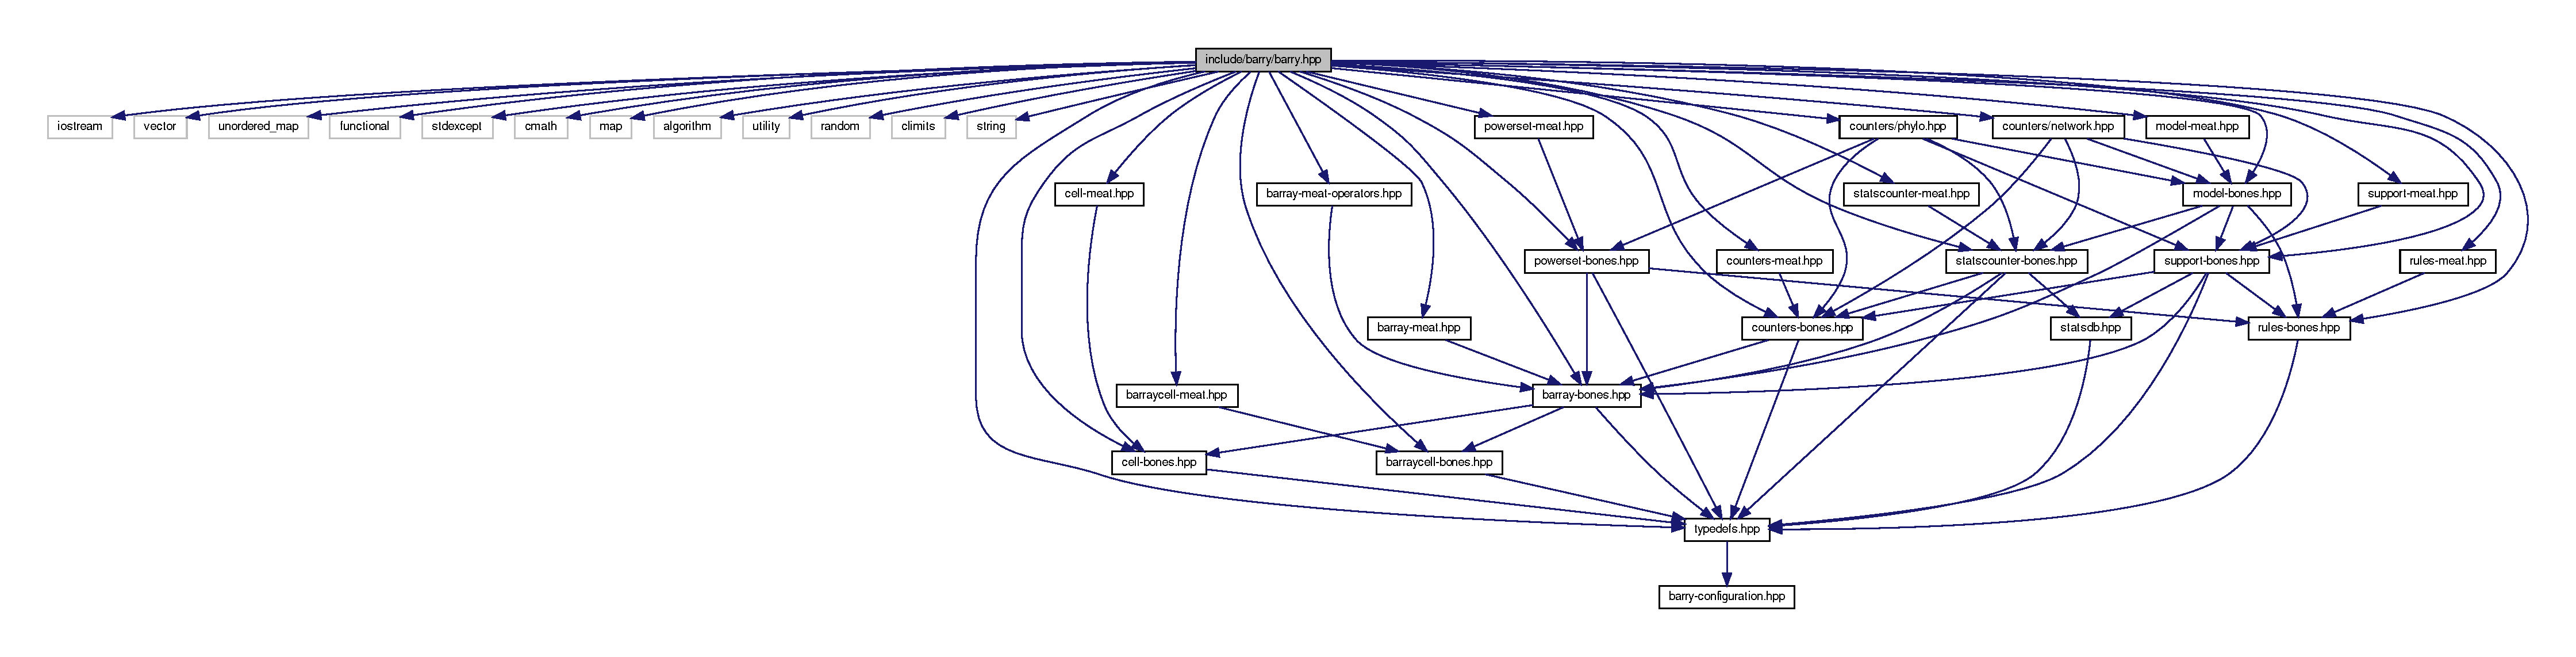
\includegraphics[width=350pt]{barry_8hpp__incl}
\end{center}
\end{figure}
This graph shows which files directly or indirectly include this file\+:\nopagebreak
\begin{figure}[H]
\begin{center}
\leavevmode
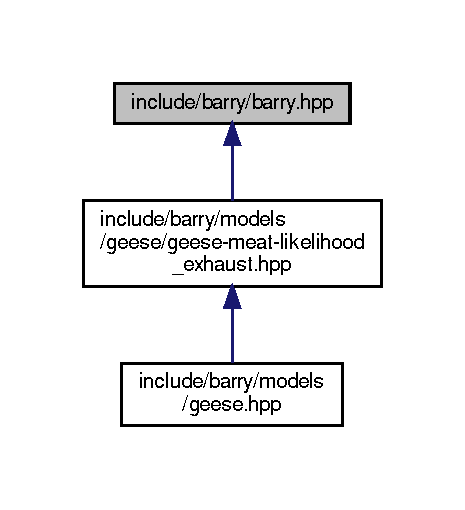
\includegraphics[width=251pt]{barry_8hpp__dep__incl}
\end{center}
\end{figure}
\subsection*{Classes}
\begin{DoxyCompactItemize}
\item 
class \hyperlink{classbarry_1_1_cell}{barry\+::\+Cell$<$ Cell\+\_\+\+Type $>$}
\begin{DoxyCompactList}\small\item\em \hyperlink{classbarry_1_1_entries}{Entries} in \hyperlink{classbarry_1_1_b_array}{B\+Array}. For now, it only has two members\+: \end{DoxyCompactList}\item 
class \hyperlink{classbarry_1_1_entries}{barry\+::\+Entries$<$ Cell\+\_\+\+Type $>$}
\begin{DoxyCompactList}\small\item\em A wrapper class to store {\ttfamily source}, {\ttfamily target}, {\ttfamily val} from a {\ttfamily \hyperlink{classbarry_1_1_b_array}{B\+Array}} object. \end{DoxyCompactList}\item 
struct \hyperlink{structbarry_1_1vec_hasher}{barry\+::vec\+Hasher$<$ T $>$}
\item 
class \hyperlink{classbarry_1_1_b_array}{barry\+::\+B\+Array$<$ Cell\+\_\+\+Type, Data\+\_\+\+Type $>$}
\item 
class \hyperlink{classbarry_1_1_counter}{barry\+::\+Counter$<$ Array\+\_\+\+Type, Data\+\_\+\+Type $>$}
\begin{DoxyCompactList}\small\item\em A counter function based on change statistics. \end{DoxyCompactList}\item 
class \hyperlink{classbarry_1_1_cell}{barry\+::\+Cell$<$ Cell\+\_\+\+Type $>$}
\begin{DoxyCompactList}\small\item\em \hyperlink{classbarry_1_1_entries}{Entries} in \hyperlink{classbarry_1_1_b_array}{B\+Array}. For now, it only has two members\+: \end{DoxyCompactList}\item 
class \hyperlink{classbarry_1_1_b_array_cell}{barry\+::\+B\+Array\+Cell$<$ Cell\+\_\+\+Type, Data\+\_\+\+Type $>$}
\item 
class \hyperlink{classbarry_1_1_counter}{barry\+::\+Counter$<$ Array\+\_\+\+Type, Data\+\_\+\+Type $>$}
\begin{DoxyCompactList}\small\item\em A counter function based on change statistics. \end{DoxyCompactList}\item 
class \hyperlink{classbarry_1_1_counters}{barry\+::\+Counters$<$ Array\+\_\+\+Type, Data\+\_\+\+Type $>$}
\begin{DoxyCompactList}\small\item\em Vector of counters. \end{DoxyCompactList}\item 
class \hyperlink{classbarry_1_1_freq_table}{barry\+::\+Freq\+Table$<$ T $>$}
\begin{DoxyCompactList}\small\item\em Database of statistics. \end{DoxyCompactList}\item 
class \hyperlink{classbarry_1_1_stats_counter}{barry\+::\+Stats\+Counter$<$ Array\+\_\+\+Type, Data\+\_\+\+Type $>$}
\begin{DoxyCompactList}\small\item\em Count stats for a single Array. \end{DoxyCompactList}\item 
class \hyperlink{classbarry_1_1_rule}{barry\+::\+Rule$<$ Array\+\_\+\+Type, Data\+\_\+\+Type $>$}
\begin{DoxyCompactList}\small\item\em \hyperlink{classbarry_1_1_rule}{Rule} for determining if a cell should be included in a sequence. \end{DoxyCompactList}\item 
class \hyperlink{classbarry_1_1_rules}{barry\+::\+Rules$<$ Array\+\_\+\+Type, Data\+\_\+\+Type $>$}
\begin{DoxyCompactList}\small\item\em Vector of objects of class \hyperlink{classbarry_1_1_rule}{Rule}. \end{DoxyCompactList}\item 
class \hyperlink{classbarry_1_1_support}{barry\+::\+Support$<$ Array\+\_\+\+Type, Data\+\_\+\+Counter\+\_\+\+Type, Data\+\_\+\+Rule\+\_\+\+Type $>$}
\begin{DoxyCompactList}\small\item\em Compute the support of sufficient statistics. \end{DoxyCompactList}\item 
class \hyperlink{classbarry_1_1_cell_seq}{barry\+::\+Cell\+Seq$<$ Array\+\_\+\+Type, Data\+\_\+\+Type $>$}
\begin{DoxyCompactList}\small\item\em Sequence of cells indices. \end{DoxyCompactList}\item 
class \hyperlink{classbarry_1_1_power_set}{barry\+::\+Power\+Set$<$ Array\+\_\+\+Type, Data\+\_\+\+Rule\+\_\+\+Type $>$}
\item 
class \hyperlink{classbarry_1_1_model}{barry\+::\+Model$<$ Array\+\_\+\+Type, Data\+\_\+\+Counter\+\_\+\+Type, Data\+\_\+\+Rule\+\_\+\+Type $>$}
\begin{DoxyCompactList}\small\item\em General framework for discrete exponential models. This class allows generating discrete exponential models in the form of a linear exponential model\+: \[ \frac{ \exp{\left(\theta^{\mbox{t}}c(A)\right)} }{ \sum_{A'\in \mathcal{A}}\exp{\left(\theta^{\mbox{t}}c(A')\right)} } \]. \end{DoxyCompactList}\item 
class \hyperlink{classbarry_1_1counters_1_1network_1_1_network_data}{barry\+::counters\+::network\+::\+Network\+Data}
\begin{DoxyCompactList}\small\item\em Data class for Networks. \end{DoxyCompactList}\item 
class \hyperlink{classbarry_1_1counters_1_1network_1_1_net_counter_data}{barry\+::counters\+::network\+::\+Net\+Counter\+Data}
\begin{DoxyCompactList}\small\item\em Data class used to store arbitrary uint or double vectors. \end{DoxyCompactList}\item 
class \hyperlink{classbarry_1_1counters_1_1phylo_1_1_node_data}{barry\+::counters\+::phylo\+::\+Node\+Data}
\begin{DoxyCompactList}\small\item\em Data definition for the {\ttfamily Phylo\+Array} class. \end{DoxyCompactList}\end{DoxyCompactItemize}
\subsection*{Namespaces}
\begin{DoxyCompactItemize}
\item 
 \hyperlink{namespacebarry}{barry}
\begin{DoxyCompactList}\small\item\em barry\+: Your go-\/to motif accountant \end{DoxyCompactList}\item 
 \hyperlink{namespacebarry_1_1_c_h_e_c_k}{barry\+::\+C\+H\+E\+CK}
\begin{DoxyCompactList}\small\item\em Integer constants used to specify which cell should be check. \end{DoxyCompactList}\item 
 \hyperlink{namespacebarry_1_1_e_x_i_s_t_s}{barry\+::\+E\+X\+I\+S\+TS}
\begin{DoxyCompactList}\small\item\em Integer constants used to specify which cell should be check to exist or not. \end{DoxyCompactList}\item 
 \hyperlink{namespacebarry_1_1counters}{barry\+::counters}
\item 
 \hyperlink{namespacebarry_1_1counters_1_1network}{barry\+::counters\+::network}
\item 
 \hyperlink{namespacebarry_1_1counters_1_1phylo}{barry\+::counters\+::phylo}
\end{DoxyCompactItemize}
\subsection*{Macros}
\begin{DoxyCompactItemize}
\item 
\#define \hyperlink{barry_8hpp_ae7fbc217bad33cff559b1fc41375a8ff}{C\+O\+U\+N\+T\+E\+R\+\_\+\+F\+U\+N\+C\+T\+I\+ON}(a)
\item 
\#define \hyperlink{barry_8hpp_a0dd594d2194ac0aa72b14cc42077331b}{C\+O\+U\+N\+T\+E\+R\+\_\+\+L\+A\+M\+B\+DA}(a)
\item 
\#define \hyperlink{barry_8hpp_aca4359c3356b25fb710d4dbc93d8d5a8}{R\+U\+L\+E\+\_\+\+F\+U\+N\+C\+T\+I\+ON}(a)
\item 
\#define \hyperlink{barry_8hpp_a65e3788fca9f405ff460ff7cfbad63f3}{R\+U\+L\+E\+\_\+\+L\+A\+M\+B\+DA}(a)
\end{DoxyCompactItemize}
\subsection*{Typedefs}
\begin{DoxyCompactItemize}
\item 
typedef unsigned int \hyperlink{namespacebarry_a11dfc53ddb4672278319aa04f1e09a6c}{barry\+::uint}
\item 
typedef std\+::vector$<$ std\+::pair$<$ std\+::vector$<$ double $>$, \hyperlink{typedefs_8hpp_a91ad9478d81a7aaf2593e8d9c3d06a14}{uint} $>$ $>$ \hyperlink{namespacebarry_a3e2d8c3b6cf602107559d4237d9f1315}{barry\+::\+Counts\+\_\+type}
\item 
{\footnotesize template$<$typename Cell\+\_\+\+Type $>$ }\\using \hyperlink{namespacebarry_a741876d7060484e80a9f2b9d128d2c8d}{barry\+::\+Row\+\_\+type} = \hyperlink{barry-configuration_8hpp_a1bb64c776ba5e9fc373665103b1a1772}{Map}$<$ \hyperlink{typedefs_8hpp_a91ad9478d81a7aaf2593e8d9c3d06a14}{uint}, \hyperlink{class_cell}{Cell}$<$ Cell\+\_\+\+Type $>$ $>$
\item 
{\footnotesize template$<$typename Cell\+\_\+\+Type $>$ }\\using \hyperlink{namespacebarry_ac328592ccff774bb3614f2cae43cffd7}{barry\+::\+Col\+\_\+type} = \hyperlink{barry-configuration_8hpp_a1bb64c776ba5e9fc373665103b1a1772}{Map}$<$ \hyperlink{typedefs_8hpp_a91ad9478d81a7aaf2593e8d9c3d06a14}{uint}, \hyperlink{class_cell}{Cell}$<$ Cell\+\_\+\+Type $>$ $\ast$$>$
\item 
{\footnotesize template$<$typename Ta  = double, typename Tb  = uint$>$ }\\using \hyperlink{namespacebarry_a2f0d3aab1d67e4c8eaeab9022e16139f}{barry\+::\+Map\+Vec\+\_\+type} = std\+::unordered\+\_\+map$<$ std\+::vector$<$ Ta $>$, Tb, \hyperlink{structvec_hasher}{vec\+Hasher}$<$ Ta $>$ $>$
\item 
typedef std\+::vector$<$ \hyperlink{typedefs_8hpp_a91ad9478d81a7aaf2593e8d9c3d06a14}{uint} $>$ \hyperlink{namespacebarry_1_1counters_1_1phylo_a6ecc0d8ab76f8dc2db152221a8e9e95a}{barry\+::counters\+::phylo\+::\+Phylo\+Counter\+Data}
\item 
typedef std\+::vector$<$ std\+::pair$<$ \hyperlink{typedefs_8hpp_a91ad9478d81a7aaf2593e8d9c3d06a14}{uint}, \hyperlink{typedefs_8hpp_a91ad9478d81a7aaf2593e8d9c3d06a14}{uint} $>$ $>$ \hyperlink{namespacebarry_1_1counters_1_1phylo_a5da540950bcf3372bcedb17a5b23667c}{barry\+::counters\+::phylo\+::\+Phylo\+Rule\+Data}
\end{DoxyCompactItemize}
\begin{Indent}\textbf{ Configuration M\+A\+C\+R\+OS}\par
{\em These are mostly related to performance. The definitions follow\+:


\begin{DoxyItemize}
\item {\ttfamily B\+A\+R\+R\+Y\+\_\+\+U\+S\+E\+\_\+\+U\+N\+O\+R\+D\+E\+R\+E\+D\+\_\+\+M\+AP} If specified, then barry is compiled using {\ttfamily std\+::unordered\+\_\+map}. Otherwise it will use {\ttfamily std\+::map} for the arrays.
\item {\ttfamily B\+A\+R\+R\+Y\+\_\+\+U\+S\+E\+\_\+\+S\+A\+F\+E\+\_\+\+E\+XP} When specified, it will multiply all likelihoods in {\ttfamily \hyperlink{class_model}{Model}} by (1/-\/100)/(1/-\/100) so that numerical overflows are avoided.
\item {\ttfamily B\+A\+R\+R\+Y\+\_\+\+C\+H\+E\+C\+K\+\_\+\+F\+I\+N\+I\+TE} When specified, it will introduce a macro 
\end{DoxyItemize}}\begin{DoxyCompactItemize}
\item 
{\footnotesize template$<$typename Ta , typename Tb $>$ }\\using \hyperlink{namespacebarry_a979a04835a9855ff2054c383c569c89e}{barry\+::\+Map} = std\+::map$<$ Ta, Tb $>$
\end{DoxyCompactItemize}
\end{Indent}
\textbf{ }\par
\begin{DoxyCompactItemize}
\item 
{\footnotesize template$<$typename Array\+\_\+\+Type , typename Data\+\_\+\+Type $>$ }\\using \hyperlink{namespacebarry_abaaae3200da8e4b7faac3c04fe9c3081}{barry\+::\+Counter\+\_\+fun\+\_\+type} = std\+::function$<$ double(const Array\+\_\+\+Type $\ast$, \hyperlink{typedefs_8hpp_a91ad9478d81a7aaf2593e8d9c3d06a14}{uint}, \hyperlink{typedefs_8hpp_a91ad9478d81a7aaf2593e8d9c3d06a14}{uint}, Data\+\_\+\+Type $\ast$)$>$
\begin{DoxyCompactList}\small\item\em \hyperlink{classbarry_1_1_counter}{Counter} and rule functions. \end{DoxyCompactList}\item 
{\footnotesize template$<$typename Array\+\_\+\+Type , typename Data\+\_\+\+Type $>$ }\\using \hyperlink{namespacebarry_aefd7e6d4ba228e2ce1074d075c512178}{barry\+::\+Rule\+\_\+fun\+\_\+type} = std\+::function$<$ bool(const Array\+\_\+\+Type $\ast$, \hyperlink{typedefs_8hpp_a91ad9478d81a7aaf2593e8d9c3d06a14}{uint}, \hyperlink{typedefs_8hpp_a91ad9478d81a7aaf2593e8d9c3d06a14}{uint}, Data\+\_\+\+Type $\ast$)$>$
\end{DoxyCompactItemize}

\begin{Indent}\textbf{ Convenient typedefs for network objects.}\par
\begin{DoxyCompactItemize}
\item 
typedef \hyperlink{class_b_array}{B\+Array}$<$ double, \hyperlink{class_network_data}{Network\+Data} $>$ \hyperlink{namespacebarry_1_1counters_1_1network_a440182967e1ba465e90a4b1d07e3a366}{barry\+::counters\+::network\+::\+Network}
\item 
typedef \hyperlink{class_counter}{Counter}$<$ \hyperlink{network_8hpp_ad0e1efde7782396b9f93c16ce892af05}{Network}, \hyperlink{class_net_counter_data}{Net\+Counter\+Data} $>$ \hyperlink{namespacebarry_1_1counters_1_1network_a067bd9de04608fc2e1586324d3864a45}{barry\+::counters\+::network\+::\+Net\+Counter}
\item 
typedef \hyperlink{class_counters}{Counters}$<$ \hyperlink{network_8hpp_ad0e1efde7782396b9f93c16ce892af05}{Network}, \hyperlink{class_net_counter_data}{Net\+Counter\+Data} $>$ \hyperlink{namespacebarry_1_1counters_1_1network_aa72fdb34752ac24167a06ee196a8fff6}{barry\+::counters\+::network\+::\+Net\+Counters}
\item 
typedef \hyperlink{class_support}{Support}$<$ \hyperlink{network_8hpp_ad0e1efde7782396b9f93c16ce892af05}{Network}, \hyperlink{class_net_counter_data}{Net\+Counter\+Data} $>$ \hyperlink{namespacebarry_1_1counters_1_1network_a4d30be7f465efd7d218f0264f8386b32}{barry\+::counters\+::network\+::\+Net\+Support}
\item 
typedef \hyperlink{class_stats_counter}{Stats\+Counter}$<$ \hyperlink{network_8hpp_ad0e1efde7782396b9f93c16ce892af05}{Network}, \hyperlink{class_net_counter_data}{Net\+Counter\+Data} $>$ \hyperlink{namespacebarry_1_1counters_1_1network_ae26c399917113fe280b3f2859376b8b9}{barry\+::counters\+::network\+::\+Net\+Stats\+Counter}
\item 
typedef \hyperlink{class_model}{Model}$<$ \hyperlink{network_8hpp_ad0e1efde7782396b9f93c16ce892af05}{Network}, \hyperlink{class_net_counter_data}{Net\+Counter\+Data} $>$ \hyperlink{namespacebarry_1_1counters_1_1network_a3ab1ee0750d4a5b0f92253874e055358}{barry\+::counters\+::network\+::\+Net\+Model}
\item 
typedef \hyperlink{class_rule}{Rule}$<$ \hyperlink{network_8hpp_ad0e1efde7782396b9f93c16ce892af05}{Network}, bool $>$ \hyperlink{namespacebarry_1_1counters_1_1network_afbd2c2a61931e69dd5f668c421e87a6f}{barry\+::counters\+::network\+::\+Net\+Rule}
\item 
typedef \hyperlink{class_rules}{Rules}$<$ \hyperlink{network_8hpp_ad0e1efde7782396b9f93c16ce892af05}{Network}, bool $>$ \hyperlink{namespacebarry_1_1counters_1_1network_adbdb20b3ce883777da2364984ea10c56}{barry\+::counters\+::network\+::\+Net\+Rules}
\end{DoxyCompactItemize}
\end{Indent}
\begin{Indent}\textbf{ Convenient typedefs for Node objects.}\par
\begin{DoxyCompactItemize}
\item 
typedef \hyperlink{class_b_array}{B\+Array}$<$ \hyperlink{typedefs_8hpp_a91ad9478d81a7aaf2593e8d9c3d06a14}{uint}, \hyperlink{class_node_data}{Node\+Data} $>$ \hyperlink{namespacebarry_1_1counters_1_1phylo_abd293bf65e494e903639fb5fb2c91604}{barry\+::counters\+::phylo\+::\+Phylo\+Array}
\item 
typedef \hyperlink{class_counter}{Counter}$<$ \hyperlink{phylo_8hpp_a777255ae3149368254234a1bddecb601}{Phylo\+Array}, \hyperlink{phylo_8hpp_adccc07602cc07d6c62a6851478bec99a}{Phylo\+Counter\+Data} $>$ \hyperlink{namespacebarry_1_1counters_1_1phylo_a6523924ce3465c5b212584c57664f953}{barry\+::counters\+::phylo\+::\+Phylo\+Counter}
\item 
typedef \hyperlink{class_counters}{Counters}$<$ \hyperlink{phylo_8hpp_a777255ae3149368254234a1bddecb601}{Phylo\+Array}, \hyperlink{phylo_8hpp_adccc07602cc07d6c62a6851478bec99a}{Phylo\+Counter\+Data} $>$ \hyperlink{namespacebarry_1_1counters_1_1phylo_a4e401ffe66d04091343dcffaf915f8c3}{barry\+::counters\+::phylo\+::\+Phylo\+Counters}
\item 
typedef \hyperlink{class_rule}{Rule}$<$ \hyperlink{phylo_8hpp_a777255ae3149368254234a1bddecb601}{Phylo\+Array}, \hyperlink{phylo_8hpp_ad7d1052d3cdcf6286b6d7907d1ec1eaf}{Phylo\+Rule\+Data} $>$ \hyperlink{namespacebarry_1_1counters_1_1phylo_a46a7015a86c3c1f9df301fb181ccd82c}{barry\+::counters\+::phylo\+::\+Phylo\+Rule}
\item 
typedef \hyperlink{class_rules}{Rules}$<$ \hyperlink{phylo_8hpp_a777255ae3149368254234a1bddecb601}{Phylo\+Array}, \hyperlink{phylo_8hpp_ad7d1052d3cdcf6286b6d7907d1ec1eaf}{Phylo\+Rule\+Data} $>$ \hyperlink{namespacebarry_1_1counters_1_1phylo_a7c915b4eab922a92797db96a7e8917c4}{barry\+::counters\+::phylo\+::\+Phylo\+Rules}
\item 
typedef \hyperlink{class_support}{Support}$<$ \hyperlink{phylo_8hpp_a777255ae3149368254234a1bddecb601}{Phylo\+Array}, \hyperlink{phylo_8hpp_adccc07602cc07d6c62a6851478bec99a}{Phylo\+Counter\+Data}, \hyperlink{phylo_8hpp_ad7d1052d3cdcf6286b6d7907d1ec1eaf}{Phylo\+Rule\+Data} $>$ \hyperlink{namespacebarry_1_1counters_1_1phylo_a29ed06e87d808c2e7d333aa00a0643b5}{barry\+::counters\+::phylo\+::\+Phylo\+Support}
\item 
typedef \hyperlink{class_stats_counter}{Stats\+Counter}$<$ \hyperlink{phylo_8hpp_a777255ae3149368254234a1bddecb601}{Phylo\+Array}, \hyperlink{phylo_8hpp_adccc07602cc07d6c62a6851478bec99a}{Phylo\+Counter\+Data} $>$ \hyperlink{namespacebarry_1_1counters_1_1phylo_abfefb6cff81a19d278b306a79cc011a3}{barry\+::counters\+::phylo\+::\+Phylo\+Stats\+Counter}
\item 
typedef \hyperlink{class_model}{Model}$<$ \hyperlink{phylo_8hpp_a777255ae3149368254234a1bddecb601}{Phylo\+Array}, \hyperlink{phylo_8hpp_adccc07602cc07d6c62a6851478bec99a}{Phylo\+Counter\+Data}, \hyperlink{phylo_8hpp_ad7d1052d3cdcf6286b6d7907d1ec1eaf}{Phylo\+Rule\+Data} $>$ \hyperlink{namespacebarry_1_1counters_1_1phylo_ad32b4186e3bab93119df225fddc3c609}{barry\+::counters\+::phylo\+::\+Phylo\+Model}
\item 
typedef \hyperlink{class_power_set}{Power\+Set}$<$ \hyperlink{phylo_8hpp_a777255ae3149368254234a1bddecb601}{Phylo\+Array}, \hyperlink{phylo_8hpp_ad7d1052d3cdcf6286b6d7907d1ec1eaf}{Phylo\+Rule\+Data} $>$ \hyperlink{namespacebarry_1_1counters_1_1phylo_ae89de0bf34247cac5b080aeb29b25239}{barry\+::counters\+::phylo\+::\+Phylo\+Power\+Set}
\end{DoxyCompactItemize}
\end{Indent}
\subsection*{Functions}
\begin{DoxyCompactItemize}
\item 
{\footnotesize template$<$typename T $>$ }\\T \hyperlink{namespacebarry_a0343fb4152724d5fa1ffa00d4b6182d9}{barry\+::vec\+\_\+inner\+\_\+prod} (const std\+::vector$<$ T $>$ \&a, const std\+::vector$<$ T $>$ \&b)
\item 
{\footnotesize template$<$typename Cell\+\_\+\+Type , typename Data\+\_\+\+Type $>$ }\\void \hyperlink{namespacebarry_a4ec765fc621c31c4ce712443cc4610c3}{barry\+::checkdim\+\_\+} (const \hyperlink{class_b_array}{B\+Array}$<$ Cell\+\_\+\+Type, Data\+\_\+\+Type $>$ \&lhs, const \hyperlink{class_b_array}{B\+Array}$<$ Cell\+\_\+\+Type, Data\+\_\+\+Type $>$ \&rhs)
\item 
{\footnotesize template$<$typename Array\+\_\+\+Type , typename Data\+\_\+\+Type $>$ }\\bool \hyperlink{namespacebarry_afb5a6f58fa7969d3027468e393eecd51}{barry\+::rule\+\_\+fun\+\_\+default} (const Array\+\_\+\+Type $\ast$array, \hyperlink{typedefs_8hpp_a91ad9478d81a7aaf2593e8d9c3d06a14}{uint} i, \hyperlink{typedefs_8hpp_a91ad9478d81a7aaf2593e8d9c3d06a14}{uint} j, Data\+\_\+\+Type $\ast$dat)
\item 
{\footnotesize template$<$typename Array\+\_\+\+Type , typename Data\+\_\+\+Type $>$ }\\bool \hyperlink{namespacebarry_a1cb28b501bc7f88c0b3d68d51ad672e1}{barry\+::default\+\_\+rule} (const Array\+\_\+\+Type $\ast$A, \hyperlink{typedefs_8hpp_a91ad9478d81a7aaf2593e8d9c3d06a14}{uint} i, \hyperlink{typedefs_8hpp_a91ad9478d81a7aaf2593e8d9c3d06a14}{uint} j, Data\+\_\+\+Type $\ast$)
\item 
{\footnotesize template$<$typename Array\+\_\+\+Type , typename Data\+\_\+\+Type $>$ }\\bool \hyperlink{namespacebarry_adec8d64df14ef90c3e94445e791eaa92}{barry\+::sequence\+\_\+rule\+\_\+zero\+\_\+diag} (const Array\+\_\+\+Type $\ast$A, \hyperlink{typedefs_8hpp_a91ad9478d81a7aaf2593e8d9c3d06a14}{uint} i, \hyperlink{typedefs_8hpp_a91ad9478d81a7aaf2593e8d9c3d06a14}{uint} j, Data\+\_\+\+Type $\ast$)
\item 
{\footnotesize template$<$typename Array\+\_\+\+Type , typename Data\+\_\+\+Type $>$ }\\bool \hyperlink{namespacebarry_a2889c6210e2711e33c34ca9c8b5de7d9}{barry\+::sequence\+\_\+rule\+\_\+lower\+\_\+tri} (const Array\+\_\+\+Type $\ast$A, \hyperlink{typedefs_8hpp_a91ad9478d81a7aaf2593e8d9c3d06a14}{uint} i, \hyperlink{typedefs_8hpp_a91ad9478d81a7aaf2593e8d9c3d06a14}{uint} j, Data\+\_\+\+Type $\ast$)
\item 
{\footnotesize template$<$typename Array\+\_\+\+Type , typename Data\+\_\+\+Type $>$ }\\bool \hyperlink{namespacebarry_a1433970b34e5904f846a0aa41abef448}{barry\+::sequence\+\_\+rule\+\_\+upper\+\_\+tri} (const Array\+\_\+\+Type $\ast$A, \hyperlink{typedefs_8hpp_a91ad9478d81a7aaf2593e8d9c3d06a14}{uint} i, \hyperlink{typedefs_8hpp_a91ad9478d81a7aaf2593e8d9c3d06a14}{uint} j, Data\+\_\+\+Type $\ast$)
\item 
double \hyperlink{namespacebarry_a822db820c95822d0e7a51728d9b9858d}{barry\+::update\+\_\+normalizing\+\_\+constant} (const std\+::vector$<$ double $>$ \&params, const \hyperlink{typedefs_8hpp_aee40fa17c1fddb63dd1f2b1470ade95b}{Counts\+\_\+type} \&support)
\item 
double \hyperlink{namespacebarry_a1dcc0a46544cc9733ca8ee5619ef6d20}{barry\+::likelihood\+\_\+} (const std\+::vector$<$ double $>$ \&target\+\_\+stats, const std\+::vector$<$ double $>$ \&params, const double normalizing\+\_\+constant, bool log\+\_\+=false)
\item 
{\footnotesize template$<$typename Array\+\_\+\+Type $>$ }\\std\+::vector$<$ double $>$ \hyperlink{namespacebarry_a22bfc7c4a1f5b5922edfd1101b8ffe3d}{barry\+::keygen\+\_\+default} (const Array\+\_\+\+Type \&Array\+\_\+)
\begin{DoxyCompactList}\small\item\em Array Hasher class (used for computing support) \end{DoxyCompactList}\end{DoxyCompactItemize}
\textbf{ }\par
\begin{DoxyCompactItemize}
\item 
{\footnotesize template$<$typename T $>$ }\\bool \hyperlink{namespacebarry_afbdb85734a7793890ea4268ea114858e}{barry\+::vec\+\_\+equal} (const std\+::vector$<$ T $>$ \&a, const std\+::vector$<$ T $>$ \&b)
\begin{DoxyCompactList}\small\item\em Compares if -\/a-\/ and -\/b-\/ are equal. \end{DoxyCompactList}\item 
{\footnotesize template$<$typename T $>$ }\\bool \hyperlink{namespacebarry_a24c4bd4a99dd82edf66c2d3b645dca08}{barry\+::vec\+\_\+equal\+\_\+approx} (const std\+::vector$<$ T $>$ \&a, const std\+::vector$<$ T $>$ \&b, double eps=1e-\/10)
\end{DoxyCompactItemize}

\begin{Indent}\textbf{ Counters for network models}\par
{\em 
\begin{DoxyParams}{Parameters}
{\em counters} & A pointer to a {\ttfamily Net\+Counters} object ({\ttfamily \hyperlink{class_counters}{Counters}}$<${\ttfamily Network}, {\ttfamily \hyperlink{class_net_counter_data}{Net\+Counter\+Data}}$>$). \\
\hline
\end{DoxyParams}
}\begin{DoxyCompactItemize}
\item 
void \hyperlink{namespacebarry_1_1counters_1_1network_ace52a65ee587dfe7b5e815de70350581}{barry\+::counters\+::network\+::counter\+\_\+edges} (\hyperlink{network_8hpp_a174d872a0e267d33daf4d345fab537a3}{Net\+Counters} $\ast$counters)
\begin{DoxyCompactList}\small\item\em Number of edges. \end{DoxyCompactList}\item 
void \hyperlink{namespacebarry_1_1counters_1_1network_abb12a5ddff5be1b860139a1a9bc3ff87}{barry\+::counters\+::network\+::counter\+\_\+isolates} (\hyperlink{network_8hpp_a174d872a0e267d33daf4d345fab537a3}{Net\+Counters} $\ast$counters)
\begin{DoxyCompactList}\small\item\em Number of isolated vertices. \end{DoxyCompactList}\item 
void \hyperlink{namespacebarry_1_1counters_1_1network_a668c4f3b6abba62e113ae7e382d4b63a}{barry\+::counters\+::network\+::counter\+\_\+mutual} (\hyperlink{network_8hpp_a174d872a0e267d33daf4d345fab537a3}{Net\+Counters} $\ast$counters)
\begin{DoxyCompactList}\small\item\em Number of mutual ties. \end{DoxyCompactList}\item 
void \hyperlink{namespacebarry_1_1counters_1_1network_ac1cf7a400dacb5fd40750ba4a0c00e81}{barry\+::counters\+::network\+::counter\+\_\+istar2} (\hyperlink{network_8hpp_a174d872a0e267d33daf4d345fab537a3}{Net\+Counters} $\ast$counters)
\item 
void \hyperlink{namespacebarry_1_1counters_1_1network_acbeff158b43d56c1fbf76f8c18891f9b}{barry\+::counters\+::network\+::counter\+\_\+ostar2} (\hyperlink{network_8hpp_a174d872a0e267d33daf4d345fab537a3}{Net\+Counters} $\ast$counters)
\item 
void \hyperlink{namespacebarry_1_1counters_1_1network_a5b6fdd52d0fca0ca994f6ba619123265}{barry\+::counters\+::network\+::counter\+\_\+ttriads} (\hyperlink{network_8hpp_a174d872a0e267d33daf4d345fab537a3}{Net\+Counters} $\ast$counters)
\item 
void \hyperlink{namespacebarry_1_1counters_1_1network_af04b15d38a744b0e741005c44b581368}{barry\+::counters\+::network\+::counter\+\_\+ctriads} (\hyperlink{network_8hpp_a174d872a0e267d33daf4d345fab537a3}{Net\+Counters} $\ast$counters)
\item 
void \hyperlink{namespacebarry_1_1counters_1_1network_a91e3daed40ea0514e0ede00ab303a738}{barry\+::counters\+::network\+::counter\+\_\+density} (\hyperlink{network_8hpp_a174d872a0e267d33daf4d345fab537a3}{Net\+Counters} $\ast$counters)
\item 
void \hyperlink{namespacebarry_1_1counters_1_1network_a27ece7e2bbf1ca87810c5ffbdfcce9fc}{barry\+::counters\+::network\+::counter\+\_\+idegree15} (\hyperlink{network_8hpp_a174d872a0e267d33daf4d345fab537a3}{Net\+Counters} $\ast$counters)
\item 
void \hyperlink{namespacebarry_1_1counters_1_1network_af4ab196a242dd233010b342712fe0449}{barry\+::counters\+::network\+::counter\+\_\+odegree15} (\hyperlink{network_8hpp_a174d872a0e267d33daf4d345fab537a3}{Net\+Counters} $\ast$counters)
\item 
void \hyperlink{namespacebarry_1_1counters_1_1network_a0150bbe24de4218a40c0880e55c73e9e}{barry\+::counters\+::network\+::counter\+\_\+absdiff} (\hyperlink{network_8hpp_a174d872a0e267d33daf4d345fab537a3}{Net\+Counters} $\ast$counters, \hyperlink{typedefs_8hpp_a91ad9478d81a7aaf2593e8d9c3d06a14}{uint} attr\+\_\+id, double alpha=1.\+0)
\begin{DoxyCompactList}\small\item\em Sum of absolute attribute difference between ego and alter. \end{DoxyCompactList}\item 
void \hyperlink{namespacebarry_1_1counters_1_1network_a2050eea4ac26f5e10483622633081962}{barry\+::counters\+::network\+::counter\+\_\+diff} (\hyperlink{network_8hpp_a174d872a0e267d33daf4d345fab537a3}{Net\+Counters} $\ast$counters, \hyperlink{typedefs_8hpp_a91ad9478d81a7aaf2593e8d9c3d06a14}{uint} attr\+\_\+id, double alpha=1.\+0, double tail\+\_\+head=true)
\begin{DoxyCompactList}\small\item\em Sum of attribute difference between ego and alter to pow(alpha) \end{DoxyCompactList}\item 
\hyperlink{namespacebarry_1_1counters_1_1network_a7649cd035af193258a69058aea425941}{barry\+::counters\+::network\+::\+N\+E\+T\+W\+O\+R\+K\+\_\+\+C\+O\+U\+N\+T\+ER} (init\+\_\+single\+\_\+attr)
\item 
void \hyperlink{namespacebarry_1_1counters_1_1network_a42073ab360a9f796126662927acc5470}{barry\+::counters\+::network\+::counter\+\_\+nodeicov} (\hyperlink{network_8hpp_a174d872a0e267d33daf4d345fab537a3}{Net\+Counters} $\ast$counters, \hyperlink{typedefs_8hpp_a91ad9478d81a7aaf2593e8d9c3d06a14}{uint} attr\+\_\+id)
\item 
void \hyperlink{namespacebarry_1_1counters_1_1network_a61b287d49772a5bfa3d11d42f70ec1d8}{barry\+::counters\+::network\+::counter\+\_\+nodeocov} (\hyperlink{network_8hpp_a174d872a0e267d33daf4d345fab537a3}{Net\+Counters} $\ast$counters, \hyperlink{typedefs_8hpp_a91ad9478d81a7aaf2593e8d9c3d06a14}{uint} attr\+\_\+id)
\item 
void \hyperlink{namespacebarry_1_1counters_1_1network_a0f18e2af090591c3f47c95849ec324da}{barry\+::counters\+::network\+::counter\+\_\+nodecov} (\hyperlink{network_8hpp_a174d872a0e267d33daf4d345fab537a3}{Net\+Counters} $\ast$counters, \hyperlink{typedefs_8hpp_a91ad9478d81a7aaf2593e8d9c3d06a14}{uint} attr\+\_\+id)
\item 
void \hyperlink{namespacebarry_1_1counters_1_1network_a2333b5893d1ba684925be6855bc33868}{barry\+::counters\+::network\+::counter\+\_\+nodematch} (\hyperlink{network_8hpp_a174d872a0e267d33daf4d345fab537a3}{Net\+Counters} $\ast$counters, \hyperlink{typedefs_8hpp_a91ad9478d81a7aaf2593e8d9c3d06a14}{uint} attr\+\_\+id)
\item 
void \hyperlink{namespacebarry_1_1counters_1_1network_a460e9b4cd736d8ab02ebeb6f84e3e80d}{barry\+::counters\+::network\+::counter\+\_\+idegree} (\hyperlink{network_8hpp_a174d872a0e267d33daf4d345fab537a3}{Net\+Counters} $\ast$counters, std\+::vector$<$ \hyperlink{typedefs_8hpp_a91ad9478d81a7aaf2593e8d9c3d06a14}{uint} $>$ d)
\begin{DoxyCompactList}\small\item\em Counts number of vertices with a given in-\/degree. \end{DoxyCompactList}\item 
void \hyperlink{namespacebarry_1_1counters_1_1network_adb3a690ba6de839767b66f8bda088e2e}{barry\+::counters\+::network\+::counter\+\_\+odegree} (\hyperlink{network_8hpp_a174d872a0e267d33daf4d345fab537a3}{Net\+Counters} $\ast$counters, std\+::vector$<$ \hyperlink{typedefs_8hpp_a91ad9478d81a7aaf2593e8d9c3d06a14}{uint} $>$ d)
\begin{DoxyCompactList}\small\item\em Counts number of vertices with a given out-\/degree. \end{DoxyCompactList}\item 
void \hyperlink{namespacebarry_1_1counters_1_1network_a3d7953d9b68c547fc0d02cc1f6fadb23}{barry\+::counters\+::network\+::counter\+\_\+degree} (\hyperlink{network_8hpp_a174d872a0e267d33daf4d345fab537a3}{Net\+Counters} $\ast$counters, std\+::vector$<$ \hyperlink{typedefs_8hpp_a91ad9478d81a7aaf2593e8d9c3d06a14}{uint} $>$ d)
\begin{DoxyCompactList}\small\item\em Counts number of vertices with a given out-\/degree. \end{DoxyCompactList}\end{DoxyCompactItemize}
\end{Indent}
\begin{Indent}\textbf{ Rules for network models}\par
{\em 
\begin{DoxyParams}{Parameters}
{\em rules} & A pointer to a {\ttfamily Net\+Rules} object ({\ttfamily \hyperlink{class_rules}{Rules}}$<${\ttfamily Network}, {\ttfamily bool}$>$). \\
\hline
\end{DoxyParams}
}\begin{DoxyCompactItemize}
\item 
void \hyperlink{namespacebarry_1_1counters_1_1network_a19680c70c20a093a84b6cc71a2597510}{barry\+::counters\+::network\+::rules\+\_\+zerodiag} (\hyperlink{network_8hpp_a6002c13f2cfcd506080a917d6464ab53}{Net\+Rules} $\ast$rules)
\begin{DoxyCompactList}\small\item\em Number of edges. \end{DoxyCompactList}\end{DoxyCompactItemize}
\end{Indent}
\begin{Indent}\textbf{ Counters for phylogenetic modeling.}\par
{\em 
\begin{DoxyParams}{Parameters}
{\em counters} & A pointer to a {\ttfamily Phylo\+Counters} object ({\ttfamily \hyperlink{class_counters}{Counters}}$<${\ttfamily Phylo\+Array}, {\ttfamily Phylo\+Counter\+Data}$>$). \\
\hline
\end{DoxyParams}
}\begin{DoxyCompactItemize}
\item 
void \hyperlink{namespacebarry_1_1counters_1_1phylo_ae1e599324d656660ce8730b77efcbcce}{barry\+::counters\+::phylo\+::counter\+\_\+overall\+\_\+gains} (\hyperlink{phylo_8hpp_a7f579c2548e28d17881691a3abe7ecb5}{Phylo\+Counters} $\ast$counters, bool duplication=true)
\begin{DoxyCompactList}\small\item\em Overall functional gains. \end{DoxyCompactList}\item 
void \hyperlink{namespacebarry_1_1counters_1_1phylo_afc1215e596c2f5a5e3b6f39273427a9a}{barry\+::counters\+::phylo\+::counter\+\_\+gains} (\hyperlink{phylo_8hpp_a7f579c2548e28d17881691a3abe7ecb5}{Phylo\+Counters} $\ast$counters, std\+::vector$<$ \hyperlink{typedefs_8hpp_a91ad9478d81a7aaf2593e8d9c3d06a14}{uint} $>$ nfun, bool duplication=true)
\begin{DoxyCompactList}\small\item\em Functional gains for a specific function ({\ttfamily nfun}). \end{DoxyCompactList}\item 
void \hyperlink{namespacebarry_1_1counters_1_1phylo_a1a2118168c3e375edf94fc6b53969a6b}{barry\+::counters\+::phylo\+::counter\+\_\+gains\+\_\+k\+\_\+offspring} (\hyperlink{phylo_8hpp_a7f579c2548e28d17881691a3abe7ecb5}{Phylo\+Counters} $\ast$counters, std\+::vector$<$ \hyperlink{typedefs_8hpp_a91ad9478d81a7aaf2593e8d9c3d06a14}{uint} $>$ nfun, \hyperlink{typedefs_8hpp_a91ad9478d81a7aaf2593e8d9c3d06a14}{uint} k=1u, bool duplication=true)
\begin{DoxyCompactList}\small\item\em Functional gains for a specific function ({\ttfamily nfun}). \end{DoxyCompactList}\item 
void \hyperlink{namespacebarry_1_1counters_1_1phylo_a680cd7516f66f06eb8a27d8b252b53ed}{barry\+::counters\+::phylo\+::counter\+\_\+genes\+\_\+changing} (\hyperlink{phylo_8hpp_a7f579c2548e28d17881691a3abe7ecb5}{Phylo\+Counters} $\ast$counters, bool duplication=true)
\begin{DoxyCompactList}\small\item\em Keeps track of how many genes are changing (either 0, 1, or 2 if dealing with regular trees.) \end{DoxyCompactList}\item 
void \hyperlink{namespacebarry_1_1counters_1_1phylo_a79ccde09af0d3d47b1a3162a16bc4597}{barry\+::counters\+::phylo\+::counter\+\_\+overall\+\_\+loss} (\hyperlink{phylo_8hpp_a7f579c2548e28d17881691a3abe7ecb5}{Phylo\+Counters} $\ast$counters, bool duplication=true)
\begin{DoxyCompactList}\small\item\em Overall functional loss. \end{DoxyCompactList}\item 
void \hyperlink{namespacebarry_1_1counters_1_1phylo_a80949b65fbe734d854742306065914bf}{barry\+::counters\+::phylo\+::counter\+\_\+maxfuns} (\hyperlink{phylo_8hpp_a7f579c2548e28d17881691a3abe7ecb5}{Phylo\+Counters} $\ast$counters, \hyperlink{typedefs_8hpp_a91ad9478d81a7aaf2593e8d9c3d06a14}{uint} lb, \hyperlink{typedefs_8hpp_a91ad9478d81a7aaf2593e8d9c3d06a14}{uint} ub, bool duplication=true)
\begin{DoxyCompactList}\small\item\em Cap the number of functions per gene. \end{DoxyCompactList}\item 
void \hyperlink{namespacebarry_1_1counters_1_1phylo_affbd49d13928ece0a2f100261375d2a7}{barry\+::counters\+::phylo\+::counter\+\_\+loss} (\hyperlink{phylo_8hpp_a7f579c2548e28d17881691a3abe7ecb5}{Phylo\+Counters} $\ast$counters, std\+::vector$<$ \hyperlink{typedefs_8hpp_a91ad9478d81a7aaf2593e8d9c3d06a14}{uint} $>$ nfun, bool duplication=true)
\begin{DoxyCompactList}\small\item\em Total count of losses for an specific function. \end{DoxyCompactList}\item 
void \hyperlink{namespacebarry_1_1counters_1_1phylo_abeaaaa150b98e55f7bc242810fa1230a}{barry\+::counters\+::phylo\+::counter\+\_\+overall\+\_\+changes} (\hyperlink{phylo_8hpp_a7f579c2548e28d17881691a3abe7ecb5}{Phylo\+Counters} $\ast$counters, bool duplication=true)
\begin{DoxyCompactList}\small\item\em Total number of changes. Use this statistic to account for \char`\"{}preservation\char`\"{}. \end{DoxyCompactList}\item 
void \hyperlink{namespacebarry_1_1counters_1_1phylo_ad36131d4405a758fa200fd29932f49ea}{barry\+::counters\+::phylo\+::counter\+\_\+subfun} (\hyperlink{phylo_8hpp_a7f579c2548e28d17881691a3abe7ecb5}{Phylo\+Counters} $\ast$counters, \hyperlink{typedefs_8hpp_a91ad9478d81a7aaf2593e8d9c3d06a14}{uint} nfunA, \hyperlink{typedefs_8hpp_a91ad9478d81a7aaf2593e8d9c3d06a14}{uint} nfunB, bool duplication=true)
\begin{DoxyCompactList}\small\item\em Total count of Sub-\/functionalization events. \end{DoxyCompactList}\item 
void \hyperlink{namespacebarry_1_1counters_1_1phylo_a002286f13261eb4633c6dc9e6fc1212b}{barry\+::counters\+::phylo\+::counter\+\_\+cogain} (\hyperlink{phylo_8hpp_a7f579c2548e28d17881691a3abe7ecb5}{Phylo\+Counters} $\ast$counters, \hyperlink{typedefs_8hpp_a91ad9478d81a7aaf2593e8d9c3d06a14}{uint} nfunA, \hyperlink{typedefs_8hpp_a91ad9478d81a7aaf2593e8d9c3d06a14}{uint} nfunB, bool duplication=true)
\begin{DoxyCompactList}\small\item\em Co-\/evolution (joint gain or loss) \end{DoxyCompactList}\item 
void \hyperlink{namespacebarry_1_1counters_1_1phylo_ae4ace7c30011a6d7047a94fd0ddf2df2}{barry\+::counters\+::phylo\+::counter\+\_\+longest} (\hyperlink{phylo_8hpp_a7f579c2548e28d17881691a3abe7ecb5}{Phylo\+Counters} $\ast$counters)
\begin{DoxyCompactList}\small\item\em Longest branch mutates (either by gain or by loss) \end{DoxyCompactList}\item 
void \hyperlink{namespacebarry_1_1counters_1_1phylo_a4cf48d44538ec0646783e29e89027838}{barry\+::counters\+::phylo\+::counter\+\_\+neofun} (\hyperlink{phylo_8hpp_a7f579c2548e28d17881691a3abe7ecb5}{Phylo\+Counters} $\ast$counters, \hyperlink{typedefs_8hpp_a91ad9478d81a7aaf2593e8d9c3d06a14}{uint} nfunA, \hyperlink{typedefs_8hpp_a91ad9478d81a7aaf2593e8d9c3d06a14}{uint} nfunB, bool duplication=true)
\begin{DoxyCompactList}\small\item\em Total number of neofunctionalization events. \end{DoxyCompactList}\item 
void \hyperlink{namespacebarry_1_1counters_1_1phylo_a3394895262bbf1fd603193ef21b9ddb8}{barry\+::counters\+::phylo\+::counter\+\_\+neofun\+\_\+a2b} (\hyperlink{phylo_8hpp_a7f579c2548e28d17881691a3abe7ecb5}{Phylo\+Counters} $\ast$counters, \hyperlink{typedefs_8hpp_a91ad9478d81a7aaf2593e8d9c3d06a14}{uint} nfunA, \hyperlink{typedefs_8hpp_a91ad9478d81a7aaf2593e8d9c3d06a14}{uint} nfunB, bool duplication=true)
\begin{DoxyCompactList}\small\item\em Total number of neofunctionalization events. \end{DoxyCompactList}\end{DoxyCompactItemize}
\end{Indent}
\subsection*{Variables}
\begin{DoxyCompactItemize}
\item 
const int \hyperlink{namespacebarry_1_1_c_h_e_c_k_a604b0ef801ff768bd8561362cef579b2}{barry\+::\+C\+H\+E\+C\+K\+::\+B\+O\+TH} = -\/1
\item 
const int \hyperlink{namespacebarry_1_1_c_h_e_c_k_aa64c84acf4e28b6cb1243ccda1eec41c}{barry\+::\+C\+H\+E\+C\+K\+::\+N\+O\+NE} = 0
\item 
const int \hyperlink{namespacebarry_1_1_c_h_e_c_k_add50baad3a196b1979efbbf9e6c86913}{barry\+::\+C\+H\+E\+C\+K\+::\+O\+NE} = 1
\item 
const int \hyperlink{namespacebarry_1_1_c_h_e_c_k_a6aa56c3d8a8260d90867278d21ace4d2}{barry\+::\+C\+H\+E\+C\+K\+::\+T\+WO} = 2
\item 
const int \hyperlink{namespacebarry_1_1_e_x_i_s_t_s_aac36d54d92c9ec1d030e8c08d0594a47}{barry\+::\+E\+X\+I\+S\+T\+S\+::\+B\+O\+TH} = -\/1
\item 
const int \hyperlink{namespacebarry_1_1_e_x_i_s_t_s_a67dfa30940f84313c4936321298e5b1b}{barry\+::\+E\+X\+I\+S\+T\+S\+::\+N\+O\+NE} = 0
\item 
const int \hyperlink{namespacebarry_1_1_e_x_i_s_t_s_a9f25c9b3787f9e1cf03e28f5a6dbe725}{barry\+::\+E\+X\+I\+S\+T\+S\+::\+O\+NE} = 1
\item 
const int \hyperlink{namespacebarry_1_1_e_x_i_s_t_s_ac6cc1f304cbfc3576d15294cef82c868}{barry\+::\+E\+X\+I\+S\+T\+S\+::\+T\+WO} = 1
\item 
const int \hyperlink{namespacebarry_1_1_e_x_i_s_t_s_a95d6fdf6b1f3028fff8f2aef01f50f65}{barry\+::\+E\+X\+I\+S\+T\+S\+::\+U\+K\+N\+O\+WN} = -\/1
\item 
const int \hyperlink{namespacebarry_1_1_e_x_i_s_t_s_aa86651704b200b6bb125b289fb5b3cfc}{barry\+::\+E\+X\+I\+S\+T\+S\+::\+A\+S\+\_\+\+Z\+E\+RO} = 0
\item 
const int \hyperlink{namespacebarry_1_1_e_x_i_s_t_s_a5b06fbd1208ff2094213da0791609950}{barry\+::\+E\+X\+I\+S\+T\+S\+::\+A\+S\+\_\+\+O\+NE} = 1
\end{DoxyCompactItemize}


\subsection{Macro Definition Documentation}
\mbox{\Hypertarget{barry_8hpp_ae7fbc217bad33cff559b1fc41375a8ff}\label{barry_8hpp_ae7fbc217bad33cff559b1fc41375a8ff}} 
\index{barry.\+hpp@{barry.\+hpp}!C\+O\+U\+N\+T\+E\+R\+\_\+\+F\+U\+N\+C\+T\+I\+ON@{C\+O\+U\+N\+T\+E\+R\+\_\+\+F\+U\+N\+C\+T\+I\+ON}}
\index{C\+O\+U\+N\+T\+E\+R\+\_\+\+F\+U\+N\+C\+T\+I\+ON@{C\+O\+U\+N\+T\+E\+R\+\_\+\+F\+U\+N\+C\+T\+I\+ON}!barry.\+hpp@{barry.\+hpp}}
\subsubsection{\texorpdfstring{C\+O\+U\+N\+T\+E\+R\+\_\+\+F\+U\+N\+C\+T\+I\+ON}{COUNTER\_FUNCTION}}
{\footnotesize\ttfamily \#define C\+O\+U\+N\+T\+E\+R\+\_\+\+F\+U\+N\+C\+T\+I\+ON(\begin{DoxyParamCaption}\item[{}]{a }\end{DoxyParamCaption})}

{\bfseries Value\+:}
\begin{DoxyCode}
\textcolor{keyword}{template} <\textcolor{keyword}{typename} Array\_Type = barry::BArray<>, \textcolor{keyword}{typename} Data\_Type = \textcolor{keywordtype}{bool}> \(\backslash\)
  inline double (a) (\textcolor{keyword}{const} Array\_Type * Array, \hyperlink{typedefs_8hpp_a91ad9478d81a7aaf2593e8d9c3d06a14}{uint} i, \hyperlink{typedefs_8hpp_a91ad9478d81a7aaf2593e8d9c3d06a14}{uint} j, Data\_Type * 
      \hyperlink{class_counter_a9ebfed99a67888f80c19cabc4098bdd0}{data})\(\backslash\)
\end{DoxyCode}


Definition at line 66 of file barry.\+hpp.

\mbox{\Hypertarget{barry_8hpp_a0dd594d2194ac0aa72b14cc42077331b}\label{barry_8hpp_a0dd594d2194ac0aa72b14cc42077331b}} 
\index{barry.\+hpp@{barry.\+hpp}!C\+O\+U\+N\+T\+E\+R\+\_\+\+L\+A\+M\+B\+DA@{C\+O\+U\+N\+T\+E\+R\+\_\+\+L\+A\+M\+B\+DA}}
\index{C\+O\+U\+N\+T\+E\+R\+\_\+\+L\+A\+M\+B\+DA@{C\+O\+U\+N\+T\+E\+R\+\_\+\+L\+A\+M\+B\+DA}!barry.\+hpp@{barry.\+hpp}}
\subsubsection{\texorpdfstring{C\+O\+U\+N\+T\+E\+R\+\_\+\+L\+A\+M\+B\+DA}{COUNTER\_LAMBDA}}
{\footnotesize\ttfamily \#define C\+O\+U\+N\+T\+E\+R\+\_\+\+L\+A\+M\+B\+DA(\begin{DoxyParamCaption}\item[{}]{a }\end{DoxyParamCaption})}

{\bfseries Value\+:}
\begin{DoxyCode}
\textcolor{keyword}{template} <\textcolor{keyword}{typename} Array\_Type = barry::BArray<>, \textcolor{keyword}{typename} Data\_Type = \textcolor{keywordtype}{bool}> \(\backslash\)
  Counter\_fun\_type<Array\_Type, Data\_Type> a = \(\backslash\)
  [](\textcolor{keyword}{const} Array\_Type * Array, \hyperlink{typedefs_8hpp_a91ad9478d81a7aaf2593e8d9c3d06a14}{uint} i, \hyperlink{typedefs_8hpp_a91ad9478d81a7aaf2593e8d9c3d06a14}{uint} j, Data\_Type * \hyperlink{class_counter_a9ebfed99a67888f80c19cabc4098bdd0}{data})
\end{DoxyCode}


Definition at line 69 of file barry.\+hpp.

\mbox{\Hypertarget{barry_8hpp_aca4359c3356b25fb710d4dbc93d8d5a8}\label{barry_8hpp_aca4359c3356b25fb710d4dbc93d8d5a8}} 
\index{barry.\+hpp@{barry.\+hpp}!R\+U\+L\+E\+\_\+\+F\+U\+N\+C\+T\+I\+ON@{R\+U\+L\+E\+\_\+\+F\+U\+N\+C\+T\+I\+ON}}
\index{R\+U\+L\+E\+\_\+\+F\+U\+N\+C\+T\+I\+ON@{R\+U\+L\+E\+\_\+\+F\+U\+N\+C\+T\+I\+ON}!barry.\+hpp@{barry.\+hpp}}
\subsubsection{\texorpdfstring{R\+U\+L\+E\+\_\+\+F\+U\+N\+C\+T\+I\+ON}{RULE\_FUNCTION}}
{\footnotesize\ttfamily \#define R\+U\+L\+E\+\_\+\+F\+U\+N\+C\+T\+I\+ON(\begin{DoxyParamCaption}\item[{}]{a }\end{DoxyParamCaption})}

{\bfseries Value\+:}
\begin{DoxyCode}
\textcolor{keyword}{template} <\textcolor{keyword}{typename} Array\_Type = barry::BArray<>, \textcolor{keyword}{typename} Data\_Type = \textcolor{keywordtype}{bool}> \(\backslash\)
  inline bool (a) (\textcolor{keyword}{const} Array\_Type * Array, \hyperlink{typedefs_8hpp_a91ad9478d81a7aaf2593e8d9c3d06a14}{uint} i, \hyperlink{typedefs_8hpp_a91ad9478d81a7aaf2593e8d9c3d06a14}{uint} j, Data\_Type * 
      \hyperlink{class_counter_a9ebfed99a67888f80c19cabc4098bdd0}{data})\(\backslash\)
\end{DoxyCode}


Definition at line 73 of file barry.\+hpp.

\mbox{\Hypertarget{barry_8hpp_a65e3788fca9f405ff460ff7cfbad63f3}\label{barry_8hpp_a65e3788fca9f405ff460ff7cfbad63f3}} 
\index{barry.\+hpp@{barry.\+hpp}!R\+U\+L\+E\+\_\+\+L\+A\+M\+B\+DA@{R\+U\+L\+E\+\_\+\+L\+A\+M\+B\+DA}}
\index{R\+U\+L\+E\+\_\+\+L\+A\+M\+B\+DA@{R\+U\+L\+E\+\_\+\+L\+A\+M\+B\+DA}!barry.\+hpp@{barry.\+hpp}}
\subsubsection{\texorpdfstring{R\+U\+L\+E\+\_\+\+L\+A\+M\+B\+DA}{RULE\_LAMBDA}}
{\footnotesize\ttfamily \#define R\+U\+L\+E\+\_\+\+L\+A\+M\+B\+DA(\begin{DoxyParamCaption}\item[{}]{a }\end{DoxyParamCaption})}

{\bfseries Value\+:}
\begin{DoxyCode}
\textcolor{keyword}{template} <\textcolor{keyword}{typename} Array\_Type = barry::BArray<>, \textcolor{keyword}{typename} Data\_Type = \textcolor{keywordtype}{bool}> \(\backslash\)
  Rule\_fun\_type<Array\_Type, Data\_Type> a = \(\backslash\)
  [](\textcolor{keyword}{const} Array\_Type * Array, \hyperlink{typedefs_8hpp_a91ad9478d81a7aaf2593e8d9c3d06a14}{uint} i, \hyperlink{typedefs_8hpp_a91ad9478d81a7aaf2593e8d9c3d06a14}{uint} j, Data\_Type * \hyperlink{class_counter_a9ebfed99a67888f80c19cabc4098bdd0}{data})
\end{DoxyCode}


Definition at line 76 of file barry.\+hpp.


\hypertarget{block-bones_8hpp}{}\section{include/barry/block-\/bones.hpp File Reference}
\label{block-bones_8hpp}\index{include/barry/block-\/bones.\+hpp@{include/barry/block-\/bones.\+hpp}}
{\ttfamily \#include \char`\"{}typedefs.\+hpp\char`\"{}}\newline
Include dependency graph for block-\/bones.hpp\+:\nopagebreak
\begin{figure}[H]
\begin{center}
\leavevmode
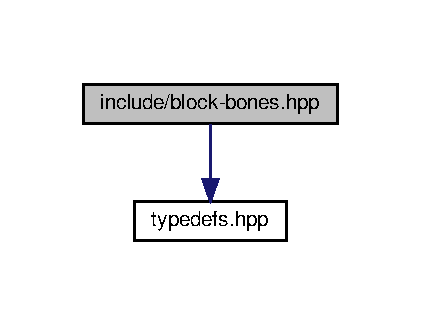
\includegraphics[width=350pt]{block-bones_8hpp__incl}
\end{center}
\end{figure}
This graph shows which files directly or indirectly include this file\+:
\nopagebreak
\begin{figure}[H]
\begin{center}
\leavevmode
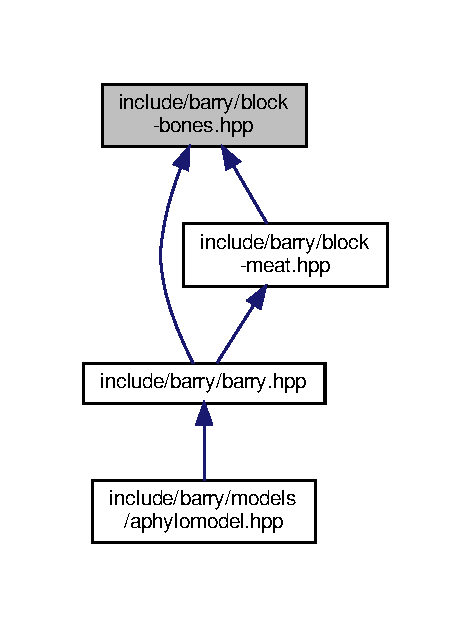
\includegraphics[width=281pt]{block-bones_8hpp__dep__incl}
\end{center}
\end{figure}
\subsection*{Classes}
\begin{DoxyCompactItemize}
\item 
class \hyperlink{class_cell_seq}{Cell\+Seq$<$ Array\+\_\+\+Type, Data\+\_\+\+Type $>$}
\begin{DoxyCompactList}\small\item\em Sequence of cells indices. \end{DoxyCompactList}\end{DoxyCompactItemize}
\subsection*{Macros}
\begin{DoxyCompactItemize}
\item 
\#define \hyperlink{barry_8hpp_ae8f9d4181425b0f42e8ff4de2449b553}{B\+A\+R\+R\+Y\+\_\+\+B\+L\+O\+C\+K\+\_\+\+B\+O\+N\+E\+S\+\_\+\+H\+PP}~1
\end{DoxyCompactItemize}
\subsection*{Functions}
\begin{DoxyCompactItemize}
\item 
{\footnotesize template$<$typename Array\+\_\+\+Type , typename Data\+\_\+\+Type $>$ }\\bool \hyperlink{block-bones_8hpp_a4aff3c5c755b16bc4634ab8d8e7fb3f6}{default\+\_\+rule} (const Array\+\_\+\+Type $\ast$A, \hyperlink{typedefs_8hpp_a91ad9478d81a7aaf2593e8d9c3d06a14}{uint} i, \hyperlink{typedefs_8hpp_a91ad9478d81a7aaf2593e8d9c3d06a14}{uint} j, Data\+\_\+\+Type $\ast$)
\end{DoxyCompactItemize}


\subsection{Macro Definition Documentation}
\mbox{\Hypertarget{barry_8hpp_ae8f9d4181425b0f42e8ff4de2449b553}\label{barry_8hpp_ae8f9d4181425b0f42e8ff4de2449b553}} 
\index{block-\/bones.\+hpp@{block-\/bones.\+hpp}!B\+A\+R\+R\+Y\+\_\+\+B\+L\+O\+C\+K\+\_\+\+B\+O\+N\+E\+S\+\_\+\+H\+PP@{B\+A\+R\+R\+Y\+\_\+\+B\+L\+O\+C\+K\+\_\+\+B\+O\+N\+E\+S\+\_\+\+H\+PP}}
\index{B\+A\+R\+R\+Y\+\_\+\+B\+L\+O\+C\+K\+\_\+\+B\+O\+N\+E\+S\+\_\+\+H\+PP@{B\+A\+R\+R\+Y\+\_\+\+B\+L\+O\+C\+K\+\_\+\+B\+O\+N\+E\+S\+\_\+\+H\+PP}!block-\/bones.\+hpp@{block-\/bones.\+hpp}}
\subsubsection{\texorpdfstring{B\+A\+R\+R\+Y\+\_\+\+B\+L\+O\+C\+K\+\_\+\+B\+O\+N\+E\+S\+\_\+\+H\+PP}{BARRY\_BLOCK\_BONES\_HPP}}
{\footnotesize\ttfamily \#define B\+A\+R\+R\+Y\+\_\+\+B\+L\+O\+C\+K\+\_\+\+B\+O\+N\+E\+S\+\_\+\+H\+PP~1}



Definition at line 7 of file barry.\+hpp.



\subsection{Function Documentation}
\mbox{\Hypertarget{block-bones_8hpp_a4aff3c5c755b16bc4634ab8d8e7fb3f6}\label{block-bones_8hpp_a4aff3c5c755b16bc4634ab8d8e7fb3f6}} 
\index{block-\/bones.\+hpp@{block-\/bones.\+hpp}!default\+\_\+rule@{default\+\_\+rule}}
\index{default\+\_\+rule@{default\+\_\+rule}!block-\/bones.\+hpp@{block-\/bones.\+hpp}}
\subsubsection{\texorpdfstring{default\+\_\+rule()}{default\_rule()}}
{\footnotesize\ttfamily template$<$typename Array\+\_\+\+Type , typename Data\+\_\+\+Type $>$ \\
bool default\+\_\+rule (\begin{DoxyParamCaption}\item[{const Array\+\_\+\+Type $\ast$}]{A,  }\item[{\hyperlink{typedefs_8hpp_a91ad9478d81a7aaf2593e8d9c3d06a14}{uint}}]{i,  }\item[{\hyperlink{typedefs_8hpp_a91ad9478d81a7aaf2593e8d9c3d06a14}{uint}}]{j,  }\item[{Data\+\_\+\+Type $\ast$}]{ }\end{DoxyParamCaption})\hspace{0.3cm}{\ttfamily [inline]}}



Definition at line 40 of file block-\/bones.\+hpp.


\hypertarget{cell-bones_8hpp}{}\section{include/cell-\/bones.hpp File Reference}
\label{cell-bones_8hpp}\index{include/cell-\/bones.\+hpp@{include/cell-\/bones.\+hpp}}
{\ttfamily \#include \char`\"{}typedefs.\+hpp\char`\"{}}\newline
Include dependency graph for cell-\/bones.hpp\+:\nopagebreak
\begin{figure}[H]
\begin{center}
\leavevmode
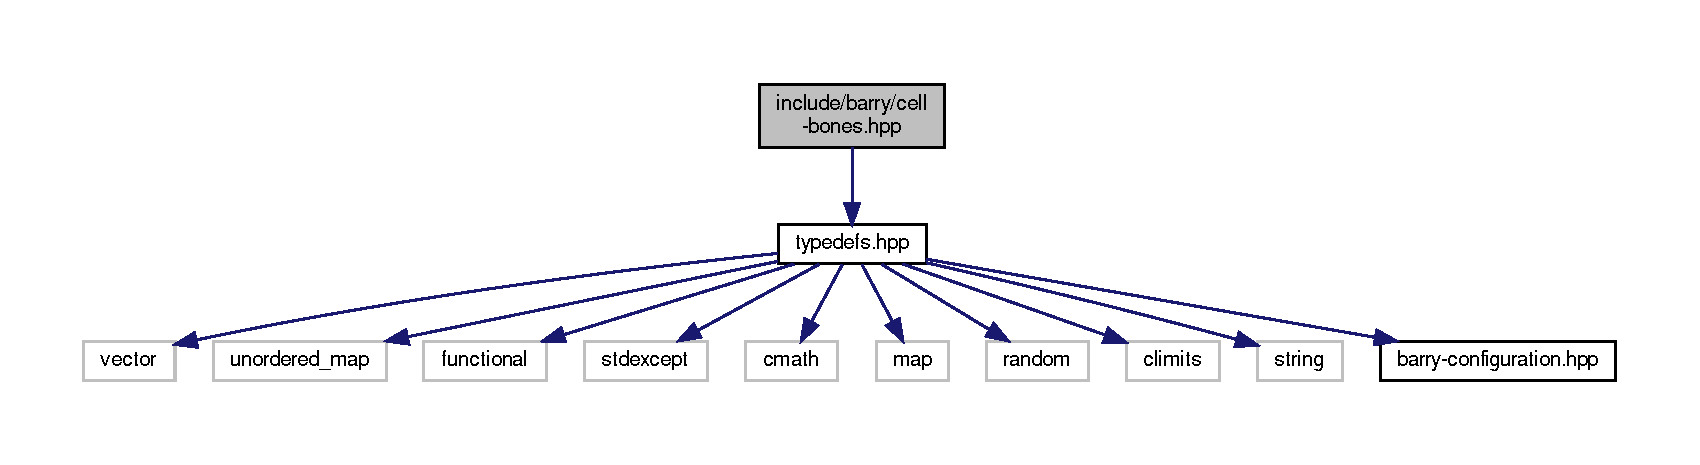
\includegraphics[width=193pt]{cell-bones_8hpp__incl}
\end{center}
\end{figure}
This graph shows which files directly or indirectly include this file\+:
\nopagebreak
\begin{figure}[H]
\begin{center}
\leavevmode
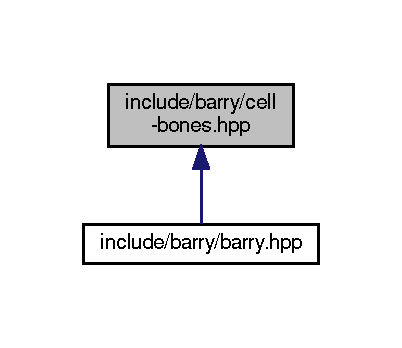
\includegraphics[width=350pt]{cell-bones_8hpp__dep__incl}
\end{center}
\end{figure}
\subsection*{Classes}
\begin{DoxyCompactItemize}
\item 
class \hyperlink{class_cell}{Cell$<$ Cell\+\_\+\+Type $>$}
\begin{DoxyCompactList}\small\item\em \hyperlink{class_entries}{Entries} in \hyperlink{class_b_array}{B\+Array}. For now, it only has two members\+: \end{DoxyCompactList}\end{DoxyCompactItemize}
\subsection*{Macros}
\begin{DoxyCompactItemize}
\item 
\#define \hyperlink{barry_8hpp_acdc5e91a788f8266c7dd182a6bf171be}{C\+E\+L\+L\+\_\+\+B\+O\+N\+E\+S\+\_\+\+H\+PP}~1
\end{DoxyCompactItemize}


\subsection{Macro Definition Documentation}
\mbox{\Hypertarget{barry_8hpp_acdc5e91a788f8266c7dd182a6bf171be}\label{barry_8hpp_acdc5e91a788f8266c7dd182a6bf171be}} 
\index{cell-\/bones.\+hpp@{cell-\/bones.\+hpp}!C\+E\+L\+L\+\_\+\+B\+O\+N\+E\+S\+\_\+\+H\+PP@{C\+E\+L\+L\+\_\+\+B\+O\+N\+E\+S\+\_\+\+H\+PP}}
\index{C\+E\+L\+L\+\_\+\+B\+O\+N\+E\+S\+\_\+\+H\+PP@{C\+E\+L\+L\+\_\+\+B\+O\+N\+E\+S\+\_\+\+H\+PP}!cell-\/bones.\+hpp@{cell-\/bones.\+hpp}}
\subsubsection{\texorpdfstring{C\+E\+L\+L\+\_\+\+B\+O\+N\+E\+S\+\_\+\+H\+PP}{CELL\_BONES\_HPP}}
{\footnotesize\ttfamily \#define C\+E\+L\+L\+\_\+\+B\+O\+N\+E\+S\+\_\+\+H\+PP~1}



Definition at line 5 of file barry.\+hpp.


\hypertarget{counters-bones_8hpp}{}\section{include/barry/counters-\/bones.hpp File Reference}
\label{counters-bones_8hpp}\index{include/barry/counters-\/bones.\+hpp@{include/barry/counters-\/bones.\+hpp}}
{\ttfamily \#include \char`\"{}typedefs.\+hpp\char`\"{}}\newline
{\ttfamily \#include \char`\"{}barray-\/bones.\+hpp\char`\"{}}\newline
Include dependency graph for counters-\/bones.hpp\+:\nopagebreak
\begin{figure}[H]
\begin{center}
\leavevmode
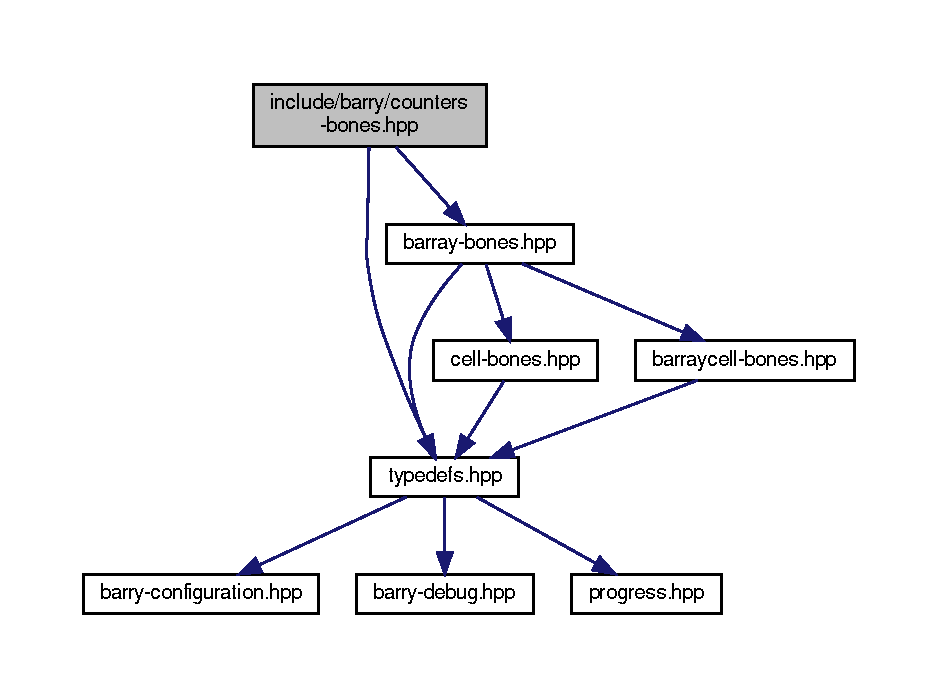
\includegraphics[width=350pt]{counters-bones_8hpp__incl}
\end{center}
\end{figure}
This graph shows which files directly or indirectly include this file\+:\nopagebreak
\begin{figure}[H]
\begin{center}
\leavevmode
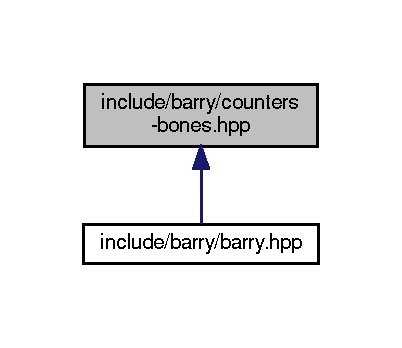
\includegraphics[width=350pt]{counters-bones_8hpp__dep__incl}
\end{center}
\end{figure}
\subsection*{Classes}
\begin{DoxyCompactItemize}
\item 
class \hyperlink{class_counter}{Counter$<$ Array\+\_\+\+Type, Data\+\_\+\+Type $>$}
\begin{DoxyCompactList}\small\item\em A counter function based on change statistics. \end{DoxyCompactList}\item 
class \hyperlink{class_counters}{Counters$<$ Array\+\_\+\+Type, Data\+\_\+\+Type $>$}
\begin{DoxyCompactList}\small\item\em Vector of counters. \end{DoxyCompactList}\end{DoxyCompactItemize}
\subsection*{Macros}
\begin{DoxyCompactItemize}
\item 
\#define \hyperlink{barry_8hpp_a1c3b1727de4f4f5d73e9040b9dd136c1}{B\+A\+R\+R\+Y\+\_\+\+C\+O\+U\+N\+T\+E\+R\+S\+\_\+\+B\+O\+N\+E\+S\+\_\+\+H\+PP}~1
\end{DoxyCompactItemize}


\subsection{Macro Definition Documentation}
\mbox{\Hypertarget{barry_8hpp_a1c3b1727de4f4f5d73e9040b9dd136c1}\label{barry_8hpp_a1c3b1727de4f4f5d73e9040b9dd136c1}} 
\index{counters-\/bones.\+hpp@{counters-\/bones.\+hpp}!B\+A\+R\+R\+Y\+\_\+\+C\+O\+U\+N\+T\+E\+R\+S\+\_\+\+B\+O\+N\+E\+S\+\_\+\+H\+PP@{B\+A\+R\+R\+Y\+\_\+\+C\+O\+U\+N\+T\+E\+R\+S\+\_\+\+B\+O\+N\+E\+S\+\_\+\+H\+PP}}
\index{B\+A\+R\+R\+Y\+\_\+\+C\+O\+U\+N\+T\+E\+R\+S\+\_\+\+B\+O\+N\+E\+S\+\_\+\+H\+PP@{B\+A\+R\+R\+Y\+\_\+\+C\+O\+U\+N\+T\+E\+R\+S\+\_\+\+B\+O\+N\+E\+S\+\_\+\+H\+PP}!counters-\/bones.\+hpp@{counters-\/bones.\+hpp}}
\subsubsection{\texorpdfstring{B\+A\+R\+R\+Y\+\_\+\+C\+O\+U\+N\+T\+E\+R\+S\+\_\+\+B\+O\+N\+E\+S\+\_\+\+H\+PP}{BARRY\_COUNTERS\_BONES\_HPP}}
{\footnotesize\ttfamily \#define B\+A\+R\+R\+Y\+\_\+\+C\+O\+U\+N\+T\+E\+R\+S\+\_\+\+B\+O\+N\+E\+S\+\_\+\+H\+PP~1}



Definition at line 5 of file barry.\+hpp.


\hypertarget{network_8hpp}{}\doxysection{include/barry/counters/network.hpp File Reference}
\label{network_8hpp}\index{include/barry/counters/network.hpp@{include/barry/counters/network.hpp}}
{\ttfamily \#include \char`\"{}network-\/css.\+hpp\char`\"{}}\newline
Include dependency graph for network.\+hpp\+:
\nopagebreak
\begin{figure}[H]
\begin{center}
\leavevmode
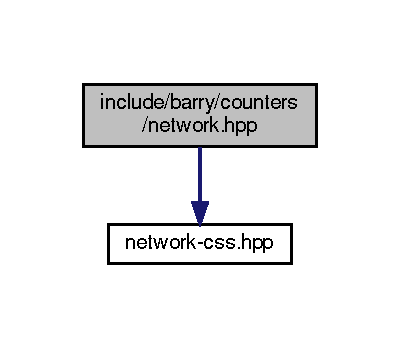
\includegraphics[width=192pt]{network_8hpp__incl}
\end{center}
\end{figure}
This graph shows which files directly or indirectly include this file\+:
\nopagebreak
\begin{figure}[H]
\begin{center}
\leavevmode
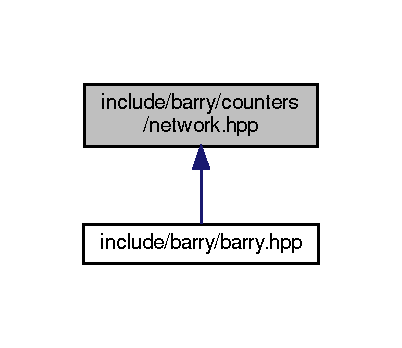
\includegraphics[width=193pt]{network_8hpp__dep__incl}
\end{center}
\end{figure}
\doxysubsection*{Classes}
\begin{DoxyCompactItemize}
\item 
class \mbox{\hyperlink{class_network_data}{Network\+Data}}
\begin{DoxyCompactList}\small\item\em Data class for Networks. \end{DoxyCompactList}\item 
class \mbox{\hyperlink{class_net_counter_data}{Net\+Counter\+Data}}
\begin{DoxyCompactList}\small\item\em Data class used to store arbitrary uint or double vectors. \end{DoxyCompactList}\end{DoxyCompactItemize}
\doxysubsection*{Macros}
\textbf{ }\par
\begin{DoxyCompactItemize}
\item 
\#define \mbox{\hyperlink{network_8hpp_aa75d9c31d709148061626dc54a07723a}{NET\+\_\+\+C\+\_\+\+DATA\+\_\+\+IDX}}(\mbox{\hyperlink{counters-meat_8hpp_aa0ecde9bec2f4c6686780ccf4f5fe835}{i}})~(\mbox{\hyperlink{counters-meat_8hpp_a6fc02db1fc3ce220c7c5e2999822ecf7}{data}}-\/$>$indices\mbox{[}\mbox{\hyperlink{counters-meat_8hpp_aa0ecde9bec2f4c6686780ccf4f5fe835}{i}}\mbox{]})
\item 
\#define \mbox{\hyperlink{network_8hpp_ad5ead8d8915b0536a4d5a6c3ef5001fb}{NET\+\_\+\+C\+\_\+\+DATA\+\_\+\+NUM}}(\mbox{\hyperlink{counters-meat_8hpp_aa0ecde9bec2f4c6686780ccf4f5fe835}{i}})~(\mbox{\hyperlink{counters-meat_8hpp_a6fc02db1fc3ce220c7c5e2999822ecf7}{data}}-\/$>$numbers\mbox{[}\mbox{\hyperlink{counters-meat_8hpp_aa0ecde9bec2f4c6686780ccf4f5fe835}{i}}\mbox{]})
\end{DoxyCompactItemize}

\begin{Indent}\textbf{ Macros for defining counters}\par
\begin{DoxyCompactItemize}
\item 
\#define \mbox{\hyperlink{network_8hpp_ad7bf24e04cb161400f56990502bda0e2}{NETWORK\+\_\+\+COUNTER}}(a)
\item 
\#define \mbox{\hyperlink{network_8hpp_a8d2a3024f1f05e716a1b4cacfe661fac}{NETWORK\+\_\+\+COUNTER\+\_\+\+LAMBDA}}(a)
\item 
\#define \mbox{\hyperlink{network_8hpp_a0e9872b5ae19d4e845e545d1f42057b8}{NETWORKDENSE\+\_\+\+COUNTER\+\_\+\+LAMBDA}}(a)
\end{DoxyCompactItemize}
\end{Indent}
\begin{Indent}\textbf{ Macros for defining rules}\par
\begin{DoxyCompactItemize}
\item 
\#define \mbox{\hyperlink{network_8hpp_a029e63cbf36397488cbd25940afb4c38}{NETWORK\+\_\+\+RULE}}(a)
\item 
\#define \mbox{\hyperlink{network_8hpp_a676ca55541b8cd4d73caca424ea7e53d}{NETWORK\+\_\+\+RULE\+\_\+\+LAMBDA}}(a)
\end{DoxyCompactItemize}
\end{Indent}
\doxysubsection*{Functions}
\begin{DoxyCompactItemize}
\item 
{\footnotesize template$<$typename Tnet  = Network$>$ }\\void \mbox{\hyperlink{group__counters-network_gaa20cbb0b2a612048d0c20bb9cabeb8e3}{counter\+\_\+edges}} (\mbox{\hyperlink{network_8hpp_a93d69933a4fa28f3460e7647ac03860d}{Net\+Counters}}$<$ Tnet $>$ $\ast$\mbox{\hyperlink{support-meat_8hpp_a782c48a908662b34845b6f654f929788}{counters}})
\begin{DoxyCompactList}\small\item\em Number of edges. \end{DoxyCompactList}\item 
{\footnotesize template$<$typename Tnet  = Network$>$ }\\void \mbox{\hyperlink{group__counters-network_ga7563764e739bd6a2021ce4ec3b26eb76}{counter\+\_\+isolates}} (\mbox{\hyperlink{network_8hpp_a93d69933a4fa28f3460e7647ac03860d}{Net\+Counters}}$<$ Tnet $>$ $\ast$\mbox{\hyperlink{support-meat_8hpp_a782c48a908662b34845b6f654f929788}{counters}})
\begin{DoxyCompactList}\small\item\em Number of isolated vertices. \end{DoxyCompactList}\item 
template$<$$>$ void \mbox{\hyperlink{group__counters-network_gadfadf92506970c5deff0c96bd3549cce}{counter\+\_\+isolates}} (\mbox{\hyperlink{network_8hpp_a93d69933a4fa28f3460e7647ac03860d}{Net\+Counters}}$<$ \mbox{\hyperlink{network_8hpp_a9ba41d6263c31a6f9a92d45bc8b2ff87}{Network\+Dense}} $>$ $\ast$\mbox{\hyperlink{support-meat_8hpp_a782c48a908662b34845b6f654f929788}{counters}})
\item 
{\footnotesize template$<$typename Tnet  = Network$>$ }\\void \mbox{\hyperlink{group__counters-network_ga1605cc66474b3b960bddd7c0adebcfc7}{counter\+\_\+mutual}} (\mbox{\hyperlink{network_8hpp_a93d69933a4fa28f3460e7647ac03860d}{Net\+Counters}}$<$ Tnet $>$ $\ast$\mbox{\hyperlink{support-meat_8hpp_a782c48a908662b34845b6f654f929788}{counters}})
\begin{DoxyCompactList}\small\item\em Number of mutual ties. \end{DoxyCompactList}\item 
{\footnotesize template$<$typename Tnet  = Network$>$ }\\void \mbox{\hyperlink{group__counters-network_ga0ca1e0394d95e7ddd1848732ef2005e9}{counter\+\_\+istar2}} (\mbox{\hyperlink{network_8hpp_a93d69933a4fa28f3460e7647ac03860d}{Net\+Counters}}$<$ Tnet $>$ $\ast$\mbox{\hyperlink{support-meat_8hpp_a782c48a908662b34845b6f654f929788}{counters}})
\item 
template$<$$>$ void \mbox{\hyperlink{group__counters-network_gabab4fe84f6bd71d96ebfb1feff1a6f66}{counter\+\_\+istar2}} (\mbox{\hyperlink{network_8hpp_a93d69933a4fa28f3460e7647ac03860d}{Net\+Counters}}$<$ \mbox{\hyperlink{network_8hpp_a9ba41d6263c31a6f9a92d45bc8b2ff87}{Network\+Dense}} $>$ $\ast$\mbox{\hyperlink{support-meat_8hpp_a782c48a908662b34845b6f654f929788}{counters}})
\item 
{\footnotesize template$<$typename Tnet  = Network$>$ }\\void \mbox{\hyperlink{group__counters-network_ga218f364352e49e462d6f152ad848f9dc}{counter\+\_\+ostar2}} (\mbox{\hyperlink{network_8hpp_a93d69933a4fa28f3460e7647ac03860d}{Net\+Counters}}$<$ Tnet $>$ $\ast$\mbox{\hyperlink{support-meat_8hpp_a782c48a908662b34845b6f654f929788}{counters}})
\item 
template$<$$>$ void \mbox{\hyperlink{group__counters-network_gad2e83eeaed6f17346ac8ac1ca64b327a}{counter\+\_\+ostar2}} (\mbox{\hyperlink{network_8hpp_a93d69933a4fa28f3460e7647ac03860d}{Net\+Counters}}$<$ \mbox{\hyperlink{network_8hpp_a9ba41d6263c31a6f9a92d45bc8b2ff87}{Network\+Dense}} $>$ $\ast$\mbox{\hyperlink{support-meat_8hpp_a782c48a908662b34845b6f654f929788}{counters}})
\item 
{\footnotesize template$<$typename Tnet  = Network$>$ }\\void \mbox{\hyperlink{group__counters-network_ga465ebcc2edcdae4ff9cd7625f886681f}{counter\+\_\+ttriads}} (\mbox{\hyperlink{network_8hpp_a93d69933a4fa28f3460e7647ac03860d}{Net\+Counters}}$<$ Tnet $>$ $\ast$\mbox{\hyperlink{support-meat_8hpp_a782c48a908662b34845b6f654f929788}{counters}})
\item 
template$<$$>$ void \mbox{\hyperlink{group__counters-network_gadadede01536081fb8b79e4d14368f946}{counter\+\_\+ttriads}} (\mbox{\hyperlink{network_8hpp_a93d69933a4fa28f3460e7647ac03860d}{Net\+Counters}}$<$ \mbox{\hyperlink{network_8hpp_a9ba41d6263c31a6f9a92d45bc8b2ff87}{Network\+Dense}} $>$ $\ast$\mbox{\hyperlink{support-meat_8hpp_a782c48a908662b34845b6f654f929788}{counters}})
\item 
{\footnotesize template$<$typename Tnet  = Network$>$ }\\void \mbox{\hyperlink{group__counters-network_ga558e4e627e5d99062d4c5546c443aabb}{counter\+\_\+ctriads}} (\mbox{\hyperlink{network_8hpp_a93d69933a4fa28f3460e7647ac03860d}{Net\+Counters}}$<$ Tnet $>$ $\ast$\mbox{\hyperlink{support-meat_8hpp_a782c48a908662b34845b6f654f929788}{counters}})
\item 
template$<$$>$ void \mbox{\hyperlink{group__counters-network_gaf3fec1692cb595e2d22205b105a8e727}{counter\+\_\+ctriads}} (\mbox{\hyperlink{network_8hpp_a93d69933a4fa28f3460e7647ac03860d}{Net\+Counters}}$<$ \mbox{\hyperlink{network_8hpp_a9ba41d6263c31a6f9a92d45bc8b2ff87}{Network\+Dense}} $>$ $\ast$\mbox{\hyperlink{support-meat_8hpp_a782c48a908662b34845b6f654f929788}{counters}})
\item 
{\footnotesize template$<$typename Tnet  = Network$>$ }\\void \mbox{\hyperlink{group__counters-network_ga54be4f2afc03d8616c60ed148219865f}{counter\+\_\+density}} (\mbox{\hyperlink{network_8hpp_a93d69933a4fa28f3460e7647ac03860d}{Net\+Counters}}$<$ Tnet $>$ $\ast$\mbox{\hyperlink{support-meat_8hpp_a782c48a908662b34845b6f654f929788}{counters}})
\item 
{\footnotesize template$<$typename Tnet  = Network$>$ }\\void \mbox{\hyperlink{group__counters-network_gaed62411a578038a5cb8e8da0ca93064f}{counter\+\_\+idegree15}} (\mbox{\hyperlink{network_8hpp_a93d69933a4fa28f3460e7647ac03860d}{Net\+Counters}}$<$ Tnet $>$ $\ast$\mbox{\hyperlink{support-meat_8hpp_a782c48a908662b34845b6f654f929788}{counters}})
\item 
template$<$$>$ void \mbox{\hyperlink{group__counters-network_ga51c01546635bbfd827174ec5900552ac}{counter\+\_\+idegree15}} (\mbox{\hyperlink{network_8hpp_a93d69933a4fa28f3460e7647ac03860d}{Net\+Counters}}$<$ \mbox{\hyperlink{network_8hpp_a9ba41d6263c31a6f9a92d45bc8b2ff87}{Network\+Dense}} $>$ $\ast$\mbox{\hyperlink{support-meat_8hpp_a782c48a908662b34845b6f654f929788}{counters}})
\item 
{\footnotesize template$<$typename Tnet  = Network$>$ }\\void \mbox{\hyperlink{group__counters-network_gac3f7b3edf5f2f648a6780ebe6505ae73}{counter\+\_\+odegree15}} (\mbox{\hyperlink{network_8hpp_a93d69933a4fa28f3460e7647ac03860d}{Net\+Counters}}$<$ Tnet $>$ $\ast$\mbox{\hyperlink{support-meat_8hpp_a782c48a908662b34845b6f654f929788}{counters}})
\item 
template$<$$>$ void \mbox{\hyperlink{group__counters-network_gad45b2c461b0ce77715410ce9d11efbe6}{counter\+\_\+odegree15}} (\mbox{\hyperlink{network_8hpp_a93d69933a4fa28f3460e7647ac03860d}{Net\+Counters}}$<$ \mbox{\hyperlink{network_8hpp_a9ba41d6263c31a6f9a92d45bc8b2ff87}{Network\+Dense}} $>$ $\ast$\mbox{\hyperlink{support-meat_8hpp_a782c48a908662b34845b6f654f929788}{counters}})
\item 
{\footnotesize template$<$typename Tnet  = Network$>$ }\\void \mbox{\hyperlink{group__counters-network_ga19fa1a8fde7be85c9304f420edd81d90}{counter\+\_\+absdiff}} (\mbox{\hyperlink{network_8hpp_a93d69933a4fa28f3460e7647ac03860d}{Net\+Counters}}$<$ Tnet $>$ $\ast$\mbox{\hyperlink{support-meat_8hpp_a782c48a908662b34845b6f654f929788}{counters}}, \mbox{\hyperlink{typedefs_8hpp_a91ad9478d81a7aaf2593e8d9c3d06a14}{uint}} attr\+\_\+id, double alpha=1.\+0)
\begin{DoxyCompactList}\small\item\em Sum of absolute attribute difference between ego and alter. \end{DoxyCompactList}\item 
{\footnotesize template$<$typename Tnet  = Network$>$ }\\void \mbox{\hyperlink{group__counters-network_ga48ad01a1af3733b904502f8b4a2ba9a7}{counter\+\_\+diff}} (\mbox{\hyperlink{network_8hpp_a93d69933a4fa28f3460e7647ac03860d}{Net\+Counters}}$<$ Tnet $>$ $\ast$\mbox{\hyperlink{support-meat_8hpp_a782c48a908662b34845b6f654f929788}{counters}}, \mbox{\hyperlink{typedefs_8hpp_a91ad9478d81a7aaf2593e8d9c3d06a14}{uint}} attr\+\_\+id, double alpha=1.\+0, double tail\+\_\+head=true)
\begin{DoxyCompactList}\small\item\em Sum of attribute difference between ego and alter to pow(alpha) \end{DoxyCompactList}\item 
\mbox{\hyperlink{group__counters-network_gad6539320de604e7c6e31e9fb152f70bd}{NETWORK\+\_\+\+COUNTER}} (init\+\_\+single\+\_\+attr)
\item 
{\footnotesize template$<$typename Tnet  = Network$>$ }\\void \mbox{\hyperlink{group__counters-network_ga8569033492c656bff9866586f12f9d4c}{counter\+\_\+nodeicov}} (\mbox{\hyperlink{network_8hpp_a93d69933a4fa28f3460e7647ac03860d}{Net\+Counters}}$<$ Tnet $>$ $\ast$\mbox{\hyperlink{support-meat_8hpp_a782c48a908662b34845b6f654f929788}{counters}}, \mbox{\hyperlink{typedefs_8hpp_a91ad9478d81a7aaf2593e8d9c3d06a14}{uint}} attr\+\_\+id)
\item 
{\footnotesize template$<$typename Tnet  = Network$>$ }\\void \mbox{\hyperlink{group__counters-network_gab4f95ef521698bd4c1868b46800513d6}{counter\+\_\+nodeocov}} (\mbox{\hyperlink{network_8hpp_a93d69933a4fa28f3460e7647ac03860d}{Net\+Counters}}$<$ Tnet $>$ $\ast$\mbox{\hyperlink{support-meat_8hpp_a782c48a908662b34845b6f654f929788}{counters}}, \mbox{\hyperlink{typedefs_8hpp_a91ad9478d81a7aaf2593e8d9c3d06a14}{uint}} attr\+\_\+id)
\item 
{\footnotesize template$<$typename Tnet  = Network$>$ }\\void \mbox{\hyperlink{group__counters-network_gaa38b17191ef9a98fc7c68cc935887550}{counter\+\_\+nodecov}} (\mbox{\hyperlink{network_8hpp_a93d69933a4fa28f3460e7647ac03860d}{Net\+Counters}}$<$ Tnet $>$ $\ast$\mbox{\hyperlink{support-meat_8hpp_a782c48a908662b34845b6f654f929788}{counters}}, \mbox{\hyperlink{typedefs_8hpp_a91ad9478d81a7aaf2593e8d9c3d06a14}{uint}} attr\+\_\+id)
\item 
{\footnotesize template$<$typename Tnet  = Network$>$ }\\void \mbox{\hyperlink{group__counters-network_ga0570512531674559bf50beaa9b1b28c2}{counter\+\_\+nodematch}} (\mbox{\hyperlink{network_8hpp_a93d69933a4fa28f3460e7647ac03860d}{Net\+Counters}}$<$ Tnet $>$ $\ast$\mbox{\hyperlink{support-meat_8hpp_a782c48a908662b34845b6f654f929788}{counters}}, \mbox{\hyperlink{typedefs_8hpp_a91ad9478d81a7aaf2593e8d9c3d06a14}{uint}} attr\+\_\+id)
\item 
{\footnotesize template$<$typename Tnet  = Network$>$ }\\void \mbox{\hyperlink{group__counters-network_gabbe3c52b9ed4649e08cbee10be2f5a4e}{counter\+\_\+idegree}} (\mbox{\hyperlink{network_8hpp_a93d69933a4fa28f3460e7647ac03860d}{Net\+Counters}}$<$ Tnet $>$ $\ast$\mbox{\hyperlink{support-meat_8hpp_a782c48a908662b34845b6f654f929788}{counters}}, std\+::vector$<$ \mbox{\hyperlink{typedefs_8hpp_a91ad9478d81a7aaf2593e8d9c3d06a14}{uint}} $>$ d)
\begin{DoxyCompactList}\small\item\em Counts number of vertices with a given in-\/degree. \end{DoxyCompactList}\item 
template$<$$>$ void \mbox{\hyperlink{group__counters-network_gabf5fddfd9b2200194527775478fa4bb3}{counter\+\_\+idegree}} (\mbox{\hyperlink{network_8hpp_a93d69933a4fa28f3460e7647ac03860d}{Net\+Counters}}$<$ \mbox{\hyperlink{network_8hpp_a9ba41d6263c31a6f9a92d45bc8b2ff87}{Network\+Dense}} $>$ $\ast$\mbox{\hyperlink{support-meat_8hpp_a782c48a908662b34845b6f654f929788}{counters}}, std\+::vector$<$ \mbox{\hyperlink{typedefs_8hpp_a91ad9478d81a7aaf2593e8d9c3d06a14}{uint}} $>$ d)
\item 
{\footnotesize template$<$typename Tnet  = Network$>$ }\\void \mbox{\hyperlink{group__counters-network_gaaae1b44d32d04b450d511d6de7f5af39}{counter\+\_\+odegree}} (\mbox{\hyperlink{network_8hpp_a93d69933a4fa28f3460e7647ac03860d}{Net\+Counters}}$<$ Tnet $>$ $\ast$\mbox{\hyperlink{support-meat_8hpp_a782c48a908662b34845b6f654f929788}{counters}}, std\+::vector$<$ \mbox{\hyperlink{typedefs_8hpp_a91ad9478d81a7aaf2593e8d9c3d06a14}{uint}} $>$ d)
\begin{DoxyCompactList}\small\item\em Counts number of vertices with a given out-\/degree. \end{DoxyCompactList}\item 
template$<$$>$ void \mbox{\hyperlink{group__counters-network_gaaed28658f06c0017211a01e134633ce5}{counter\+\_\+odegree}} (\mbox{\hyperlink{network_8hpp_a93d69933a4fa28f3460e7647ac03860d}{Net\+Counters}}$<$ \mbox{\hyperlink{network_8hpp_a9ba41d6263c31a6f9a92d45bc8b2ff87}{Network\+Dense}} $>$ $\ast$\mbox{\hyperlink{support-meat_8hpp_a782c48a908662b34845b6f654f929788}{counters}}, std\+::vector$<$ \mbox{\hyperlink{typedefs_8hpp_a91ad9478d81a7aaf2593e8d9c3d06a14}{uint}} $>$ d)
\item 
{\footnotesize template$<$typename Tnet  = Network$>$ }\\void \mbox{\hyperlink{group__counters-network_gafc27419f2beda417390bd8afb49c8189}{counter\+\_\+degree}} (\mbox{\hyperlink{network_8hpp_a93d69933a4fa28f3460e7647ac03860d}{Net\+Counters}}$<$ Tnet $>$ $\ast$\mbox{\hyperlink{support-meat_8hpp_a782c48a908662b34845b6f654f929788}{counters}}, std\+::vector$<$ \mbox{\hyperlink{typedefs_8hpp_a91ad9478d81a7aaf2593e8d9c3d06a14}{uint}} $>$ d)
\begin{DoxyCompactList}\small\item\em Counts number of vertices with a given out-\/degree. \end{DoxyCompactList}\end{DoxyCompactItemize}
\begin{Indent}\textbf{ Rules for network models}\par
{\em 
\begin{DoxyParams}{Parameters}
{\em rules} & A pointer to a {\ttfamily Net\+Rules} object ({\ttfamily \mbox{\hyperlink{class_rules}{Rules}}}$<${\ttfamily Network}, {\ttfamily bool}$>$). \\
\hline
\end{DoxyParams}
}\begin{DoxyCompactItemize}
\item 
{\footnotesize template$<$typename Tnet  = Network$>$ }\\void \mbox{\hyperlink{network_8hpp_ade7c09a084b266e48f9222c54fd12681}{rules\+\_\+zerodiag}} (\mbox{\hyperlink{network_8hpp_aa7fdf74711b0b97f984156cee30683c3}{Net\+Rules}}$<$ Tnet $>$ $\ast$\mbox{\hyperlink{support-meat_8hpp_a595e07a99f60f22a6a29e4fca291ea28}{rules}})
\begin{DoxyCompactList}\small\item\em Number of edges. \end{DoxyCompactList}\end{DoxyCompactItemize}
\end{Indent}
\doxysubsection*{Convenient typedefs for network objects.}
\begin{DoxyCompactItemize}
\item 
\#define \mbox{\hyperlink{network_8hpp_a04dccf9e770b1aeb8a788de60db7d91d}{BARRY\+\_\+\+ZERO\+\_\+\+NETWORK}}~0.\+0
\item 
\#define \mbox{\hyperlink{network_8hpp_a54e30310f12e2e7c2110c61b9fd8a68a}{BARRY\+\_\+\+ZERO\+\_\+\+NETWORK\+\_\+\+DENSE}}~0
\item 
typedef \mbox{\hyperlink{class_b_array}{BArray}}$<$ double, \mbox{\hyperlink{class_network_data}{Network\+Data}} $>$ \mbox{\hyperlink{network_8hpp_ad0e1efde7782396b9f93c16ce892af05}{Network}}
\item 
typedef \mbox{\hyperlink{class_b_array_dense}{BArray\+Dense}}$<$ int, \mbox{\hyperlink{class_network_data}{Network\+Data}} $>$ \mbox{\hyperlink{network_8hpp_a9ba41d6263c31a6f9a92d45bc8b2ff87}{Network\+Dense}}
\item 
{\footnotesize template$<$typename Tnet  = Network$>$ }\\using \mbox{\hyperlink{network_8hpp_a75ff9a7bece02dfc6d99fc2f7a35e463}{Net\+Counter}} = \mbox{\hyperlink{class_counter}{Counter}}$<$ Tnet, \mbox{\hyperlink{class_net_counter_data}{Net\+Counter\+Data}} $>$
\item 
{\footnotesize template$<$typename Tnet  = Network$>$ }\\using \mbox{\hyperlink{network_8hpp_a93d69933a4fa28f3460e7647ac03860d}{Net\+Counters}} = \mbox{\hyperlink{class_counters}{Counters}}$<$ Tnet, \mbox{\hyperlink{class_net_counter_data}{Net\+Counter\+Data}} $>$
\item 
{\footnotesize template$<$typename Tnet  = Network$>$ }\\using \mbox{\hyperlink{network_8hpp_a8e585f661c3cacbff9653516b0babf00}{Net\+Support}} = \mbox{\hyperlink{class_support}{Support}}$<$ Tnet, \mbox{\hyperlink{class_net_counter_data}{Net\+Counter\+Data}} $>$
\item 
{\footnotesize template$<$typename Tnet  = Network$>$ }\\using \mbox{\hyperlink{network_8hpp_aa601fca284af7d89c905f0077e350cc0}{Net\+Stats\+Counter}} = \mbox{\hyperlink{class_stats_counter}{Stats\+Counter}}$<$ Tnet, \mbox{\hyperlink{class_net_counter_data}{Net\+Counter\+Data}} $>$
\item 
{\footnotesize template$<$typename Tnet $>$ }\\using \mbox{\hyperlink{network_8hpp_a3689057a7a18f67f6839f3e1b2b6c140}{Net\+Model}} = \mbox{\hyperlink{class_model}{Model}}$<$ Tnet, \mbox{\hyperlink{class_net_counter_data}{Net\+Counter\+Data}} $>$
\item 
{\footnotesize template$<$typename Tnet  = Network$>$ }\\using \mbox{\hyperlink{network_8hpp_ac8c9529b68fa80139a776663a7ee43a1}{Net\+Rule}} = \mbox{\hyperlink{class_rule}{Rule}}$<$ Tnet, bool $>$
\item 
{\footnotesize template$<$typename Tnet  = Network$>$ }\\using \mbox{\hyperlink{network_8hpp_aa7fdf74711b0b97f984156cee30683c3}{Net\+Rules}} = \mbox{\hyperlink{class_rules}{Rules}}$<$ Tnet, bool $>$
\end{DoxyCompactItemize}


\doxysubsection{Macro Definition Documentation}
\mbox{\Hypertarget{network_8hpp_a04dccf9e770b1aeb8a788de60db7d91d}\label{network_8hpp_a04dccf9e770b1aeb8a788de60db7d91d}} 
\index{network.hpp@{network.hpp}!BARRY\_ZERO\_NETWORK@{BARRY\_ZERO\_NETWORK}}
\index{BARRY\_ZERO\_NETWORK@{BARRY\_ZERO\_NETWORK}!network.hpp@{network.hpp}}
\doxysubsubsection{\texorpdfstring{BARRY\_ZERO\_NETWORK}{BARRY\_ZERO\_NETWORK}}
{\footnotesize\ttfamily \#define BARRY\+\_\+\+ZERO\+\_\+\+NETWORK~0.\+0}



Definition at line 85 of file network.\+hpp.

\mbox{\Hypertarget{network_8hpp_a54e30310f12e2e7c2110c61b9fd8a68a}\label{network_8hpp_a54e30310f12e2e7c2110c61b9fd8a68a}} 
\index{network.hpp@{network.hpp}!BARRY\_ZERO\_NETWORK\_DENSE@{BARRY\_ZERO\_NETWORK\_DENSE}}
\index{BARRY\_ZERO\_NETWORK\_DENSE@{BARRY\_ZERO\_NETWORK\_DENSE}!network.hpp@{network.hpp}}
\doxysubsubsection{\texorpdfstring{BARRY\_ZERO\_NETWORK\_DENSE}{BARRY\_ZERO\_NETWORK\_DENSE}}
{\footnotesize\ttfamily \#define BARRY\+\_\+\+ZERO\+\_\+\+NETWORK\+\_\+\+DENSE~0}



Definition at line 86 of file network.\+hpp.

\mbox{\Hypertarget{network_8hpp_aa75d9c31d709148061626dc54a07723a}\label{network_8hpp_aa75d9c31d709148061626dc54a07723a}} 
\index{network.hpp@{network.hpp}!NET\_C\_DATA\_IDX@{NET\_C\_DATA\_IDX}}
\index{NET\_C\_DATA\_IDX@{NET\_C\_DATA\_IDX}!network.hpp@{network.hpp}}
\doxysubsubsection{\texorpdfstring{NET\_C\_DATA\_IDX}{NET\_C\_DATA\_IDX}}
{\footnotesize\ttfamily \#define NET\+\_\+\+C\+\_\+\+DATA\+\_\+\+IDX(\begin{DoxyParamCaption}\item[{}]{\mbox{\hyperlink{counters-meat_8hpp_aa0ecde9bec2f4c6686780ccf4f5fe835}{i}} }\end{DoxyParamCaption})~(\mbox{\hyperlink{counters-meat_8hpp_a6fc02db1fc3ce220c7c5e2999822ecf7}{data}}-\/$>$indices\mbox{[}\mbox{\hyperlink{counters-meat_8hpp_aa0ecde9bec2f4c6686780ccf4f5fe835}{i}}\mbox{]})}



Definition at line 74 of file network.\+hpp.

\mbox{\Hypertarget{network_8hpp_ad5ead8d8915b0536a4d5a6c3ef5001fb}\label{network_8hpp_ad5ead8d8915b0536a4d5a6c3ef5001fb}} 
\index{network.hpp@{network.hpp}!NET\_C\_DATA\_NUM@{NET\_C\_DATA\_NUM}}
\index{NET\_C\_DATA\_NUM@{NET\_C\_DATA\_NUM}!network.hpp@{network.hpp}}
\doxysubsubsection{\texorpdfstring{NET\_C\_DATA\_NUM}{NET\_C\_DATA\_NUM}}
{\footnotesize\ttfamily \#define NET\+\_\+\+C\+\_\+\+DATA\+\_\+\+NUM(\begin{DoxyParamCaption}\item[{}]{\mbox{\hyperlink{counters-meat_8hpp_aa0ecde9bec2f4c6686780ccf4f5fe835}{i}} }\end{DoxyParamCaption})~(\mbox{\hyperlink{counters-meat_8hpp_a6fc02db1fc3ce220c7c5e2999822ecf7}{data}}-\/$>$numbers\mbox{[}\mbox{\hyperlink{counters-meat_8hpp_aa0ecde9bec2f4c6686780ccf4f5fe835}{i}}\mbox{]})}



Definition at line 75 of file network.\+hpp.

\mbox{\Hypertarget{network_8hpp_ad7bf24e04cb161400f56990502bda0e2}\label{network_8hpp_ad7bf24e04cb161400f56990502bda0e2}} 
\index{network.hpp@{network.hpp}!NETWORK\_COUNTER@{NETWORK\_COUNTER}}
\index{NETWORK\_COUNTER@{NETWORK\_COUNTER}!network.hpp@{network.hpp}}
\doxysubsubsection{\texorpdfstring{NETWORK\_COUNTER}{NETWORK\_COUNTER}}
{\footnotesize\ttfamily \#define NETWORK\+\_\+\+COUNTER(\begin{DoxyParamCaption}\item[{}]{a }\end{DoxyParamCaption})}

{\bfseries Value\+:}
\begin{DoxyCode}{0}
\DoxyCodeLine{\textcolor{keyword}{template}<\textcolor{keyword}{typename} Tnet = Network>\(\backslash\)}
\DoxyCodeLine{inline double (a) (\textcolor{keyword}{const} Tnet \& Array, \mbox{\hyperlink{typedefs_8hpp_a91ad9478d81a7aaf2593e8d9c3d06a14}{uint}} \mbox{\hyperlink{counters-meat_8hpp_aa0ecde9bec2f4c6686780ccf4f5fe835}{i}}, \mbox{\hyperlink{typedefs_8hpp_a91ad9478d81a7aaf2593e8d9c3d06a14}{uint}} \mbox{\hyperlink{barray-meat_8hpp_abbe66f29402555d707260862a10eb56e}{j}}, \mbox{\hyperlink{class_net_counter_data}{NetCounterData}} * \mbox{\hyperlink{barray-meat_8hpp_a511ae0b1c13f95e5f08f1a0dd3da3d93}{data}})}

\end{DoxyCode}
Function for definition of a network counter function 

Definition at line 114 of file network.\+hpp.

\mbox{\Hypertarget{network_8hpp_a8d2a3024f1f05e716a1b4cacfe661fac}\label{network_8hpp_a8d2a3024f1f05e716a1b4cacfe661fac}} 
\index{network.hpp@{network.hpp}!NETWORK\_COUNTER\_LAMBDA@{NETWORK\_COUNTER\_LAMBDA}}
\index{NETWORK\_COUNTER\_LAMBDA@{NETWORK\_COUNTER\_LAMBDA}!network.hpp@{network.hpp}}
\doxysubsubsection{\texorpdfstring{NETWORK\_COUNTER\_LAMBDA}{NETWORK\_COUNTER\_LAMBDA}}
{\footnotesize\ttfamily \#define NETWORK\+\_\+\+COUNTER\+\_\+\+LAMBDA(\begin{DoxyParamCaption}\item[{}]{a }\end{DoxyParamCaption})}

{\bfseries Value\+:}
\begin{DoxyCode}{0}
\DoxyCodeLine{\mbox{\hyperlink{typedefs_8hpp_a1e12ad6cdda3588f5b2157a5ad3177d2}{Counter\_fun\_type<Tnet, NetCounterData>}} a = \(\backslash\)}
\DoxyCodeLine{    [](\textcolor{keyword}{const} Tnet \& Array, \mbox{\hyperlink{typedefs_8hpp_a91ad9478d81a7aaf2593e8d9c3d06a14}{uint}} \mbox{\hyperlink{counters-meat_8hpp_aa0ecde9bec2f4c6686780ccf4f5fe835}{i}}, \mbox{\hyperlink{typedefs_8hpp_a91ad9478d81a7aaf2593e8d9c3d06a14}{uint}} \mbox{\hyperlink{barray-meat_8hpp_abbe66f29402555d707260862a10eb56e}{j}}, \mbox{\hyperlink{class_net_counter_data}{NetCounterData}} * \mbox{\hyperlink{barray-meat_8hpp_a511ae0b1c13f95e5f08f1a0dd3da3d93}{data}})}

\end{DoxyCode}
Lambda function for definition of a network counter function 

Definition at line 119 of file network.\+hpp.

\mbox{\Hypertarget{network_8hpp_a029e63cbf36397488cbd25940afb4c38}\label{network_8hpp_a029e63cbf36397488cbd25940afb4c38}} 
\index{network.hpp@{network.hpp}!NETWORK\_RULE@{NETWORK\_RULE}}
\index{NETWORK\_RULE@{NETWORK\_RULE}!network.hpp@{network.hpp}}
\doxysubsubsection{\texorpdfstring{NETWORK\_RULE}{NETWORK\_RULE}}
{\footnotesize\ttfamily \#define NETWORK\+\_\+\+RULE(\begin{DoxyParamCaption}\item[{}]{a }\end{DoxyParamCaption})}

{\bfseries Value\+:}
\begin{DoxyCode}{0}
\DoxyCodeLine{\textcolor{keyword}{template}<\textcolor{keyword}{typename} Tnet = Network>\(\backslash\)}
\DoxyCodeLine{inline bool (a) (\textcolor{keyword}{const} Tnet \& Array, \mbox{\hyperlink{typedefs_8hpp_a91ad9478d81a7aaf2593e8d9c3d06a14}{uint}} \mbox{\hyperlink{counters-meat_8hpp_aa0ecde9bec2f4c6686780ccf4f5fe835}{i}}, \mbox{\hyperlink{typedefs_8hpp_a91ad9478d81a7aaf2593e8d9c3d06a14}{uint}} \mbox{\hyperlink{barray-meat_8hpp_abbe66f29402555d707260862a10eb56e}{j}}, \textcolor{keywordtype}{bool} * \mbox{\hyperlink{barray-meat_8hpp_a511ae0b1c13f95e5f08f1a0dd3da3d93}{data}})}

\end{DoxyCode}
Function for definition of a network counter function 

Definition at line 133 of file network.\+hpp.

\mbox{\Hypertarget{network_8hpp_a676ca55541b8cd4d73caca424ea7e53d}\label{network_8hpp_a676ca55541b8cd4d73caca424ea7e53d}} 
\index{network.hpp@{network.hpp}!NETWORK\_RULE\_LAMBDA@{NETWORK\_RULE\_LAMBDA}}
\index{NETWORK\_RULE\_LAMBDA@{NETWORK\_RULE\_LAMBDA}!network.hpp@{network.hpp}}
\doxysubsubsection{\texorpdfstring{NETWORK\_RULE\_LAMBDA}{NETWORK\_RULE\_LAMBDA}}
{\footnotesize\ttfamily \#define NETWORK\+\_\+\+RULE\+\_\+\+LAMBDA(\begin{DoxyParamCaption}\item[{}]{a }\end{DoxyParamCaption})}

{\bfseries Value\+:}
\begin{DoxyCode}{0}
\DoxyCodeLine{\mbox{\hyperlink{typedefs_8hpp_a99982bdca40c23ca6f901c8e66da78a1}{Rule\_fun\_type<Tnet, bool>}} a = \(\backslash\)}
\DoxyCodeLine{[](\textcolor{keyword}{const} Tnet \& Array, \mbox{\hyperlink{typedefs_8hpp_a91ad9478d81a7aaf2593e8d9c3d06a14}{uint}} \mbox{\hyperlink{counters-meat_8hpp_aa0ecde9bec2f4c6686780ccf4f5fe835}{i}}, \mbox{\hyperlink{typedefs_8hpp_a91ad9478d81a7aaf2593e8d9c3d06a14}{uint}} \mbox{\hyperlink{barray-meat_8hpp_abbe66f29402555d707260862a10eb56e}{j}}, \textcolor{keywordtype}{bool} * \mbox{\hyperlink{barray-meat_8hpp_a511ae0b1c13f95e5f08f1a0dd3da3d93}{data}})}

\end{DoxyCode}
Lambda function for definition of a network counter function 

Definition at line 138 of file network.\+hpp.

\mbox{\Hypertarget{network_8hpp_a0e9872b5ae19d4e845e545d1f42057b8}\label{network_8hpp_a0e9872b5ae19d4e845e545d1f42057b8}} 
\index{network.hpp@{network.hpp}!NETWORKDENSE\_COUNTER\_LAMBDA@{NETWORKDENSE\_COUNTER\_LAMBDA}}
\index{NETWORKDENSE\_COUNTER\_LAMBDA@{NETWORKDENSE\_COUNTER\_LAMBDA}!network.hpp@{network.hpp}}
\doxysubsubsection{\texorpdfstring{NETWORKDENSE\_COUNTER\_LAMBDA}{NETWORKDENSE\_COUNTER\_LAMBDA}}
{\footnotesize\ttfamily \#define NETWORKDENSE\+\_\+\+COUNTER\+\_\+\+LAMBDA(\begin{DoxyParamCaption}\item[{}]{a }\end{DoxyParamCaption})}

{\bfseries Value\+:}
\begin{DoxyCode}{0}
\DoxyCodeLine{\mbox{\hyperlink{typedefs_8hpp_a1e12ad6cdda3588f5b2157a5ad3177d2}{Counter\_fun\_type<NetworkDense, NetCounterData>}} a = \(\backslash\)}
\DoxyCodeLine{    [](\textcolor{keyword}{const} \mbox{\hyperlink{class_b_array_dense}{NetworkDense}} \& Array, \mbox{\hyperlink{typedefs_8hpp_a91ad9478d81a7aaf2593e8d9c3d06a14}{uint}} \mbox{\hyperlink{counters-meat_8hpp_aa0ecde9bec2f4c6686780ccf4f5fe835}{i}}, \mbox{\hyperlink{typedefs_8hpp_a91ad9478d81a7aaf2593e8d9c3d06a14}{uint}} \mbox{\hyperlink{barray-meat_8hpp_abbe66f29402555d707260862a10eb56e}{j}}, \mbox{\hyperlink{class_net_counter_data}{NetCounterData}} * \mbox{\hyperlink{barray-meat_8hpp_a511ae0b1c13f95e5f08f1a0dd3da3d93}{data}})}

\end{DoxyCode}


Definition at line 123 of file network.\+hpp.



\doxysubsection{Typedef Documentation}
\mbox{\Hypertarget{network_8hpp_a75ff9a7bece02dfc6d99fc2f7a35e463}\label{network_8hpp_a75ff9a7bece02dfc6d99fc2f7a35e463}} 
\index{network.hpp@{network.hpp}!NetCounter@{NetCounter}}
\index{NetCounter@{NetCounter}!network.hpp@{network.hpp}}
\doxysubsubsection{\texorpdfstring{NetCounter}{NetCounter}}
{\footnotesize\ttfamily template$<$typename Tnet  = Network$>$ \\
using \mbox{\hyperlink{network_8hpp_a75ff9a7bece02dfc6d99fc2f7a35e463}{Net\+Counter}} =  \mbox{\hyperlink{class_counter}{Counter}}$<$Tnet, \mbox{\hyperlink{class_net_counter_data}{Net\+Counter\+Data}} $>$}



Definition at line 89 of file network.\+hpp.

\mbox{\Hypertarget{network_8hpp_a93d69933a4fa28f3460e7647ac03860d}\label{network_8hpp_a93d69933a4fa28f3460e7647ac03860d}} 
\index{network.hpp@{network.hpp}!NetCounters@{NetCounters}}
\index{NetCounters@{NetCounters}!network.hpp@{network.hpp}}
\doxysubsubsection{\texorpdfstring{NetCounters}{NetCounters}}
{\footnotesize\ttfamily template$<$typename Tnet  = Network$>$ \\
using \mbox{\hyperlink{network_8hpp_a93d69933a4fa28f3460e7647ac03860d}{Net\+Counters}} =  \mbox{\hyperlink{class_counters}{Counters}}$<$Tnet, \mbox{\hyperlink{class_net_counter_data}{Net\+Counter\+Data}}$>$}



Definition at line 92 of file network.\+hpp.

\mbox{\Hypertarget{network_8hpp_a3689057a7a18f67f6839f3e1b2b6c140}\label{network_8hpp_a3689057a7a18f67f6839f3e1b2b6c140}} 
\index{network.hpp@{network.hpp}!NetModel@{NetModel}}
\index{NetModel@{NetModel}!network.hpp@{network.hpp}}
\doxysubsubsection{\texorpdfstring{NetModel}{NetModel}}
{\footnotesize\ttfamily template$<$typename Tnet $>$ \\
using \mbox{\hyperlink{network_8hpp_a3689057a7a18f67f6839f3e1b2b6c140}{Net\+Model}} =  \mbox{\hyperlink{class_model}{Model}}$<$Tnet, \mbox{\hyperlink{class_net_counter_data}{Net\+Counter\+Data}}$>$}



Definition at line 101 of file network.\+hpp.

\mbox{\Hypertarget{network_8hpp_ac8c9529b68fa80139a776663a7ee43a1}\label{network_8hpp_ac8c9529b68fa80139a776663a7ee43a1}} 
\index{network.hpp@{network.hpp}!NetRule@{NetRule}}
\index{NetRule@{NetRule}!network.hpp@{network.hpp}}
\doxysubsubsection{\texorpdfstring{NetRule}{NetRule}}
{\footnotesize\ttfamily template$<$typename Tnet  = Network$>$ \\
using \mbox{\hyperlink{network_8hpp_ac8c9529b68fa80139a776663a7ee43a1}{Net\+Rule}} =  \mbox{\hyperlink{class_rule}{Rule}}$<$Tnet, bool$>$}



Definition at line 104 of file network.\+hpp.

\mbox{\Hypertarget{network_8hpp_aa7fdf74711b0b97f984156cee30683c3}\label{network_8hpp_aa7fdf74711b0b97f984156cee30683c3}} 
\index{network.hpp@{network.hpp}!NetRules@{NetRules}}
\index{NetRules@{NetRules}!network.hpp@{network.hpp}}
\doxysubsubsection{\texorpdfstring{NetRules}{NetRules}}
{\footnotesize\ttfamily template$<$typename Tnet  = Network$>$ \\
using \mbox{\hyperlink{network_8hpp_aa7fdf74711b0b97f984156cee30683c3}{Net\+Rules}} =  \mbox{\hyperlink{class_rules}{Rules}}$<$Tnet, bool$>$}



Definition at line 107 of file network.\+hpp.

\mbox{\Hypertarget{network_8hpp_aa601fca284af7d89c905f0077e350cc0}\label{network_8hpp_aa601fca284af7d89c905f0077e350cc0}} 
\index{network.hpp@{network.hpp}!NetStatsCounter@{NetStatsCounter}}
\index{NetStatsCounter@{NetStatsCounter}!network.hpp@{network.hpp}}
\doxysubsubsection{\texorpdfstring{NetStatsCounter}{NetStatsCounter}}
{\footnotesize\ttfamily template$<$typename Tnet  = Network$>$ \\
using \mbox{\hyperlink{network_8hpp_aa601fca284af7d89c905f0077e350cc0}{Net\+Stats\+Counter}} =  \mbox{\hyperlink{class_stats_counter}{Stats\+Counter}}$<$Tnet, \mbox{\hyperlink{class_net_counter_data}{Net\+Counter\+Data}}$>$}



Definition at line 98 of file network.\+hpp.

\mbox{\Hypertarget{network_8hpp_a8e585f661c3cacbff9653516b0babf00}\label{network_8hpp_a8e585f661c3cacbff9653516b0babf00}} 
\index{network.hpp@{network.hpp}!NetSupport@{NetSupport}}
\index{NetSupport@{NetSupport}!network.hpp@{network.hpp}}
\doxysubsubsection{\texorpdfstring{NetSupport}{NetSupport}}
{\footnotesize\ttfamily template$<$typename Tnet  = Network$>$ \\
using \mbox{\hyperlink{network_8hpp_a8e585f661c3cacbff9653516b0babf00}{Net\+Support}} =  \mbox{\hyperlink{class_support}{Support}}$<$Tnet, \mbox{\hyperlink{class_net_counter_data}{Net\+Counter\+Data}} $>$}



Definition at line 95 of file network.\+hpp.

\mbox{\Hypertarget{network_8hpp_ad0e1efde7782396b9f93c16ce892af05}\label{network_8hpp_ad0e1efde7782396b9f93c16ce892af05}} 
\index{network.hpp@{network.hpp}!Network@{Network}}
\index{Network@{Network}!network.hpp@{network.hpp}}
\doxysubsubsection{\texorpdfstring{Network}{Network}}
{\footnotesize\ttfamily typedef \mbox{\hyperlink{class_b_array}{BArray}}$<$double, \mbox{\hyperlink{class_network_data}{Network\+Data}}$>$ \mbox{\hyperlink{network_8hpp_ad0e1efde7782396b9f93c16ce892af05}{Network}}}



Definition at line 82 of file network.\+hpp.

\mbox{\Hypertarget{network_8hpp_a9ba41d6263c31a6f9a92d45bc8b2ff87}\label{network_8hpp_a9ba41d6263c31a6f9a92d45bc8b2ff87}} 
\index{network.hpp@{network.hpp}!NetworkDense@{NetworkDense}}
\index{NetworkDense@{NetworkDense}!network.hpp@{network.hpp}}
\doxysubsubsection{\texorpdfstring{NetworkDense}{NetworkDense}}
{\footnotesize\ttfamily typedef \mbox{\hyperlink{class_b_array_dense}{BArray\+Dense}}$<$int, \mbox{\hyperlink{class_network_data}{Network\+Data}}$>$ \mbox{\hyperlink{network_8hpp_a9ba41d6263c31a6f9a92d45bc8b2ff87}{Network\+Dense}}}



Definition at line 83 of file network.\+hpp.



\doxysubsection{Function Documentation}
\mbox{\Hypertarget{network_8hpp_ade7c09a084b266e48f9222c54fd12681}\label{network_8hpp_ade7c09a084b266e48f9222c54fd12681}} 
\index{network.hpp@{network.hpp}!rules\_zerodiag@{rules\_zerodiag}}
\index{rules\_zerodiag@{rules\_zerodiag}!network.hpp@{network.hpp}}
\doxysubsubsection{\texorpdfstring{rules\_zerodiag()}{rules\_zerodiag()}}
{\footnotesize\ttfamily template$<$typename Tnet  = Network$>$ \\
void rules\+\_\+zerodiag (\begin{DoxyParamCaption}\item[{\mbox{\hyperlink{network_8hpp_aa7fdf74711b0b97f984156cee30683c3}{Net\+Rules}}$<$ Tnet $>$ $\ast$}]{rules }\end{DoxyParamCaption})\hspace{0.3cm}{\ttfamily [inline]}}



Number of edges. 



Definition at line 1320 of file network.\+hpp.


\hypertarget{phylo_8hpp}{}\doxysection{include/barry/counters/phylo.hpp File Reference}
\label{phylo_8hpp}\index{include/barry/counters/phylo.hpp@{include/barry/counters/phylo.hpp}}
{\ttfamily \#include \char`\"{}../counters-\/bones.\+hpp\char`\"{}}\newline
{\ttfamily \#include \char`\"{}../support-\/bones.\+hpp\char`\"{}}\newline
{\ttfamily \#include \char`\"{}../statscounter-\/bones.\+hpp\char`\"{}}\newline
{\ttfamily \#include \char`\"{}../model-\/bones.\+hpp\char`\"{}}\newline
{\ttfamily \#include \char`\"{}../powerset-\/bones.\+hpp\char`\"{}}\newline
Include dependency graph for phylo.\+hpp\+:
\nopagebreak
\begin{figure}[H]
\begin{center}
\leavevmode
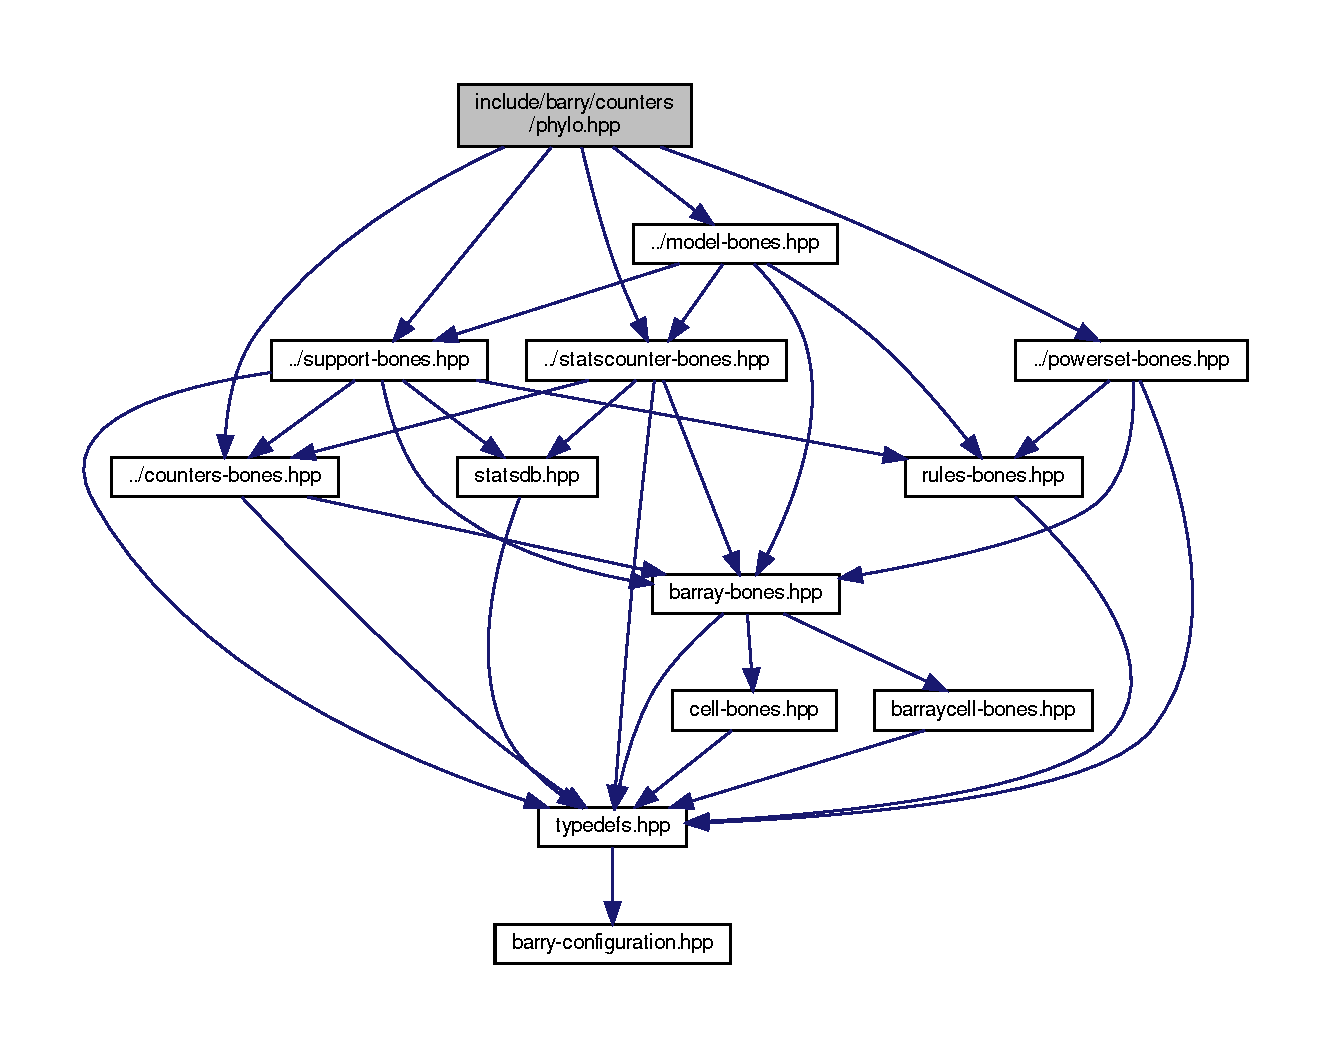
\includegraphics[width=350pt]{phylo_8hpp__incl}
\end{center}
\end{figure}
This graph shows which files directly or indirectly include this file\+:
\nopagebreak
\begin{figure}[H]
\begin{center}
\leavevmode
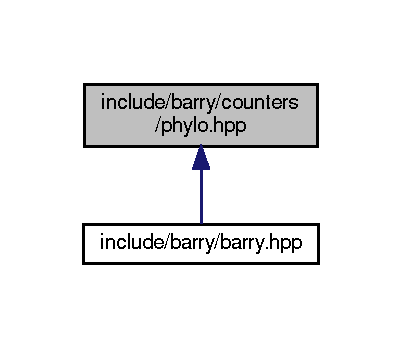
\includegraphics[width=193pt]{phylo_8hpp__dep__incl}
\end{center}
\end{figure}
\doxysubsection*{Classes}
\begin{DoxyCompactItemize}
\item 
class \mbox{\hyperlink{class_node_data}{Node\+Data}}
\begin{DoxyCompactList}\small\item\em Data definition for the {\ttfamily Phylo\+Array} class. \end{DoxyCompactList}\item 
class \mbox{\hyperlink{class_phylo_rule_dyn_data}{Phylo\+Rule\+Dyn\+Data}}
\end{DoxyCompactItemize}
\doxysubsection*{Macros}
\begin{DoxyCompactItemize}
\item 
\#define \mbox{\hyperlink{phylo_8hpp_ac89fe9750bd62a338930ea730d23d0d2}{PHYLO\+\_\+\+COUNTER\+\_\+\+LAMBDA}}(a)
\begin{DoxyCompactList}\small\item\em Extension of a simple counter. \end{DoxyCompactList}\item 
\#define \mbox{\hyperlink{phylo_8hpp_a4a7a35cddb61f74a0ec3cb3893cf78b1}{PHYLO\+\_\+\+RULE\+\_\+\+DYN\+\_\+\+LAMBDA}}(a)
\item 
\#define \mbox{\hyperlink{phylo_8hpp_a81c4979894537f31d3ecc06c5f6dd504}{PHYLO\+\_\+\+CHECK\+\_\+\+MISSING}}()
\end{DoxyCompactItemize}
\doxysubsection*{Typedefs}
\textbf{ }\par
\begin{DoxyCompactItemize}
\item 
typedef std\+::vector$<$ \mbox{\hyperlink{typedefs_8hpp_a91ad9478d81a7aaf2593e8d9c3d06a14}{uint}} $>$ \mbox{\hyperlink{phylo_8hpp_adccc07602cc07d6c62a6851478bec99a}{Phylo\+Counter\+Data}}
\item 
typedef std\+::vector$<$ std\+::pair$<$ \mbox{\hyperlink{typedefs_8hpp_a91ad9478d81a7aaf2593e8d9c3d06a14}{uint}}, \mbox{\hyperlink{typedefs_8hpp_a91ad9478d81a7aaf2593e8d9c3d06a14}{uint}} $>$ $>$ \mbox{\hyperlink{phylo_8hpp_ad7d1052d3cdcf6286b6d7907d1ec1eaf}{Phylo\+Rule\+Data}}
\end{DoxyCompactItemize}

\begin{Indent}\textbf{ Convenient typedefs for Node objects.}\par
\begin{DoxyCompactItemize}
\item 
typedef \mbox{\hyperlink{class_b_array}{BArray}}$<$ \mbox{\hyperlink{typedefs_8hpp_a91ad9478d81a7aaf2593e8d9c3d06a14}{uint}}, \mbox{\hyperlink{class_node_data}{Node\+Data}} $>$ \mbox{\hyperlink{phylo_8hpp_a777255ae3149368254234a1bddecb601}{Phylo\+Array}}
\item 
typedef \mbox{\hyperlink{class_counter}{Counter}}$<$ \mbox{\hyperlink{phylo_8hpp_a777255ae3149368254234a1bddecb601}{Phylo\+Array}}, \mbox{\hyperlink{phylo_8hpp_adccc07602cc07d6c62a6851478bec99a}{Phylo\+Counter\+Data}} $>$ \mbox{\hyperlink{phylo_8hpp_a70f35d038e8044ff5761831220d07290}{Phylo\+Counter}}
\item 
typedef \mbox{\hyperlink{class_counters}{Counters}}$<$ \mbox{\hyperlink{phylo_8hpp_a777255ae3149368254234a1bddecb601}{Phylo\+Array}}, \mbox{\hyperlink{phylo_8hpp_adccc07602cc07d6c62a6851478bec99a}{Phylo\+Counter\+Data}} $>$ \mbox{\hyperlink{phylo_8hpp_a7f579c2548e28d17881691a3abe7ecb5}{Phylo\+Counters}}
\item 
typedef \mbox{\hyperlink{class_rule}{Rule}}$<$ \mbox{\hyperlink{phylo_8hpp_a777255ae3149368254234a1bddecb601}{Phylo\+Array}}, \mbox{\hyperlink{phylo_8hpp_ad7d1052d3cdcf6286b6d7907d1ec1eaf}{Phylo\+Rule\+Data}} $>$ \mbox{\hyperlink{phylo_8hpp_a99bd6ef7a8380a0e669c1723e393429f}{Phylo\+Rule}}
\item 
typedef \mbox{\hyperlink{class_rules}{Rules}}$<$ \mbox{\hyperlink{phylo_8hpp_a777255ae3149368254234a1bddecb601}{Phylo\+Array}}, \mbox{\hyperlink{phylo_8hpp_ad7d1052d3cdcf6286b6d7907d1ec1eaf}{Phylo\+Rule\+Data}} $>$ \mbox{\hyperlink{phylo_8hpp_a297f8535006c6b28acc097dddae016c3}{Phylo\+Rules}}
\item 
typedef \mbox{\hyperlink{class_rule}{Rule}}$<$ \mbox{\hyperlink{phylo_8hpp_a777255ae3149368254234a1bddecb601}{Phylo\+Array}}, \mbox{\hyperlink{class_phylo_rule_dyn_data}{Phylo\+Rule\+Dyn\+Data}} $>$ \mbox{\hyperlink{phylo_8hpp_ad782519ef733c9b109bf465fe942b36a}{Phylo\+Rule\+Dyn}}
\item 
typedef \mbox{\hyperlink{class_rules}{Rules}}$<$ \mbox{\hyperlink{phylo_8hpp_a777255ae3149368254234a1bddecb601}{Phylo\+Array}}, \mbox{\hyperlink{class_phylo_rule_dyn_data}{Phylo\+Rule\+Dyn\+Data}} $>$ \mbox{\hyperlink{phylo_8hpp_a6c0e95789675ee382f2a42a7da14fcf9}{Phylo\+Rules\+Dyn}}
\item 
typedef \mbox{\hyperlink{class_support}{Support}}$<$ \mbox{\hyperlink{phylo_8hpp_a777255ae3149368254234a1bddecb601}{Phylo\+Array}}, \mbox{\hyperlink{phylo_8hpp_adccc07602cc07d6c62a6851478bec99a}{Phylo\+Counter\+Data}}, \mbox{\hyperlink{phylo_8hpp_ad7d1052d3cdcf6286b6d7907d1ec1eaf}{Phylo\+Rule\+Data}}, \mbox{\hyperlink{class_phylo_rule_dyn_data}{Phylo\+Rule\+Dyn\+Data}} $>$ \mbox{\hyperlink{phylo_8hpp_a7261d5284bec3ec15fe7b038399a9c5a}{Phylo\+Support}}
\item 
typedef \mbox{\hyperlink{class_stats_counter}{Stats\+Counter}}$<$ \mbox{\hyperlink{phylo_8hpp_a777255ae3149368254234a1bddecb601}{Phylo\+Array}}, \mbox{\hyperlink{phylo_8hpp_adccc07602cc07d6c62a6851478bec99a}{Phylo\+Counter\+Data}} $>$ \mbox{\hyperlink{phylo_8hpp_aca4644373aecf9b296ac8ac730470952}{Phylo\+Stats\+Counter}}
\item 
typedef \mbox{\hyperlink{class_model}{Model}}$<$ \mbox{\hyperlink{phylo_8hpp_a777255ae3149368254234a1bddecb601}{Phylo\+Array}}, \mbox{\hyperlink{phylo_8hpp_adccc07602cc07d6c62a6851478bec99a}{Phylo\+Counter\+Data}}, \mbox{\hyperlink{phylo_8hpp_ad7d1052d3cdcf6286b6d7907d1ec1eaf}{Phylo\+Rule\+Data}}, \mbox{\hyperlink{class_phylo_rule_dyn_data}{Phylo\+Rule\+Dyn\+Data}} $>$ \mbox{\hyperlink{phylo_8hpp_a3747688acf3d8e264c2ce8b07e0eb804}{Phylo\+Model}}
\item 
typedef \mbox{\hyperlink{class_power_set}{Power\+Set}}$<$ \mbox{\hyperlink{phylo_8hpp_a777255ae3149368254234a1bddecb601}{Phylo\+Array}}, \mbox{\hyperlink{phylo_8hpp_ad7d1052d3cdcf6286b6d7907d1ec1eaf}{Phylo\+Rule\+Data}} $>$ \mbox{\hyperlink{phylo_8hpp_a0d16a69c8b447a32a3aa4d4c041773cc}{Phylo\+Power\+Set}}
\end{DoxyCompactItemize}
\end{Indent}
\doxysubsection*{Functions}
\begin{DoxyCompactItemize}
\item 
std\+::string \mbox{\hyperlink{phylo_8hpp_add31e0ba346cdf08524d6da73500f846}{get\+\_\+last\+\_\+name}} (bool d)
\item 
void \mbox{\hyperlink{group__counters-phylo_gae37d65879b49c4a568e5f80795b492a5}{counter\+\_\+overall\+\_\+gains}} (\mbox{\hyperlink{phylo_8hpp_a7f579c2548e28d17881691a3abe7ecb5}{Phylo\+Counters}} $\ast$counters, bool duplication=true)
\begin{DoxyCompactList}\small\item\em Overall functional gains. \end{DoxyCompactList}\item 
void \mbox{\hyperlink{group__counters-phylo_gaf03875e668e9559a84896755e5108fc4}{counter\+\_\+gains}} (\mbox{\hyperlink{phylo_8hpp_a7f579c2548e28d17881691a3abe7ecb5}{Phylo\+Counters}} $\ast$counters, std\+::vector$<$ \mbox{\hyperlink{typedefs_8hpp_a91ad9478d81a7aaf2593e8d9c3d06a14}{uint}} $>$ nfun, bool duplication=true)
\begin{DoxyCompactList}\small\item\em Functional gains for a specific function ({\ttfamily nfun}). \end{DoxyCompactList}\item 
void \mbox{\hyperlink{group__counters-phylo_ga0403ee027de1992d33cae8cf40ad7ef3}{counter\+\_\+gains\+\_\+k\+\_\+offspring}} (\mbox{\hyperlink{phylo_8hpp_a7f579c2548e28d17881691a3abe7ecb5}{Phylo\+Counters}} $\ast$counters, std\+::vector$<$ \mbox{\hyperlink{typedefs_8hpp_a91ad9478d81a7aaf2593e8d9c3d06a14}{uint}} $>$ nfun, \mbox{\hyperlink{typedefs_8hpp_a91ad9478d81a7aaf2593e8d9c3d06a14}{uint}} k=1u, bool duplication=true)
\begin{DoxyCompactList}\small\item\em k genes gain function nfun \end{DoxyCompactList}\item 
void \mbox{\hyperlink{group__counters-phylo_ga8baaa25ef41a56b0581be6f03d27305e}{counter\+\_\+genes\+\_\+changing}} (\mbox{\hyperlink{phylo_8hpp_a7f579c2548e28d17881691a3abe7ecb5}{Phylo\+Counters}} $\ast$counters, bool duplication=true)
\begin{DoxyCompactList}\small\item\em Keeps track of how many genes are changing (either 0, 1, or 2 if dealing with regular trees.) \end{DoxyCompactList}\item 
void \mbox{\hyperlink{group__counters-phylo_gab37d32fa637cbd423d7f20dd80655d09}{counter\+\_\+prop\+\_\+genes\+\_\+changing}} (\mbox{\hyperlink{phylo_8hpp_a7f579c2548e28d17881691a3abe7ecb5}{Phylo\+Counters}} $\ast$counters, bool duplication=true)
\begin{DoxyCompactList}\small\item\em Keeps track of how many genes are changing (either 0, 1, or 2 if dealing with regular trees.) \end{DoxyCompactList}\item 
void \mbox{\hyperlink{group__counters-phylo_gadce790b84a0a7e875e543bec08194f2b}{counter\+\_\+overall\+\_\+loss}} (\mbox{\hyperlink{phylo_8hpp_a7f579c2548e28d17881691a3abe7ecb5}{Phylo\+Counters}} $\ast$counters, bool duplication=true)
\begin{DoxyCompactList}\small\item\em Overall functional loss. \end{DoxyCompactList}\item 
void \mbox{\hyperlink{group__counters-phylo_gabf517e1c04c9e08be6e32de80859c1be}{counter\+\_\+maxfuns}} (\mbox{\hyperlink{phylo_8hpp_a7f579c2548e28d17881691a3abe7ecb5}{Phylo\+Counters}} $\ast$counters, \mbox{\hyperlink{typedefs_8hpp_a91ad9478d81a7aaf2593e8d9c3d06a14}{uint}} lb, \mbox{\hyperlink{typedefs_8hpp_a91ad9478d81a7aaf2593e8d9c3d06a14}{uint}} ub, bool duplication=true)
\begin{DoxyCompactList}\small\item\em Cap the number of functions per gene. \end{DoxyCompactList}\item 
void \mbox{\hyperlink{group__counters-phylo_gab295380f631d6ecbc6147ede9e7084d8}{counter\+\_\+loss}} (\mbox{\hyperlink{phylo_8hpp_a7f579c2548e28d17881691a3abe7ecb5}{Phylo\+Counters}} $\ast$counters, std\+::vector$<$ \mbox{\hyperlink{typedefs_8hpp_a91ad9478d81a7aaf2593e8d9c3d06a14}{uint}} $>$ nfun, bool duplication=true)
\begin{DoxyCompactList}\small\item\em Total count of losses for an specific function. \end{DoxyCompactList}\item 
void \mbox{\hyperlink{group__counters-phylo_ga902c1b33b64e022b1a92f577d96eddf6}{counter\+\_\+overall\+\_\+changes}} (\mbox{\hyperlink{phylo_8hpp_a7f579c2548e28d17881691a3abe7ecb5}{Phylo\+Counters}} $\ast$counters, bool duplication=true)
\begin{DoxyCompactList}\small\item\em Total number of changes. Use this statistic to account for \char`\"{}preservation\char`\"{}. \end{DoxyCompactList}\item 
void \mbox{\hyperlink{group__counters-phylo_ga84cd89f379bfc60e36bad06eeb7063af}{counter\+\_\+subfun}} (\mbox{\hyperlink{phylo_8hpp_a7f579c2548e28d17881691a3abe7ecb5}{Phylo\+Counters}} $\ast$counters, \mbox{\hyperlink{typedefs_8hpp_a91ad9478d81a7aaf2593e8d9c3d06a14}{uint}} nfunA, \mbox{\hyperlink{typedefs_8hpp_a91ad9478d81a7aaf2593e8d9c3d06a14}{uint}} nfunB, bool duplication=true)
\begin{DoxyCompactList}\small\item\em Total count of Sub-\/functionalization events. \end{DoxyCompactList}\item 
void \mbox{\hyperlink{group__counters-phylo_ga6dda7c62f8b75ccb9fbb5d06a67810ff}{counter\+\_\+cogain}} (\mbox{\hyperlink{phylo_8hpp_a7f579c2548e28d17881691a3abe7ecb5}{Phylo\+Counters}} $\ast$counters, \mbox{\hyperlink{typedefs_8hpp_a91ad9478d81a7aaf2593e8d9c3d06a14}{uint}} nfunA, \mbox{\hyperlink{typedefs_8hpp_a91ad9478d81a7aaf2593e8d9c3d06a14}{uint}} nfunB, bool duplication=true)
\begin{DoxyCompactList}\small\item\em Co-\/evolution (joint gain or loss) \end{DoxyCompactList}\item 
void \mbox{\hyperlink{group__counters-phylo_ga41afc89ceafd9c70883b37ea20b0db8a}{counter\+\_\+longest}} (\mbox{\hyperlink{phylo_8hpp_a7f579c2548e28d17881691a3abe7ecb5}{Phylo\+Counters}} $\ast$counters)
\begin{DoxyCompactList}\small\item\em Longest branch mutates (either by gain or by loss) \end{DoxyCompactList}\item 
void \mbox{\hyperlink{group__counters-phylo_gaddc0f35b7e986425c9735c28c38aa9ed}{counter\+\_\+neofun}} (\mbox{\hyperlink{phylo_8hpp_a7f579c2548e28d17881691a3abe7ecb5}{Phylo\+Counters}} $\ast$counters, \mbox{\hyperlink{typedefs_8hpp_a91ad9478d81a7aaf2593e8d9c3d06a14}{uint}} nfunA, \mbox{\hyperlink{typedefs_8hpp_a91ad9478d81a7aaf2593e8d9c3d06a14}{uint}} nfunB, bool duplication=true)
\begin{DoxyCompactList}\small\item\em Total number of neofunctionalization events. \end{DoxyCompactList}\item 
void \mbox{\hyperlink{group__counters-phylo_ga03aec4d306a8a0ad7e356bf6b137b73f}{counter\+\_\+neofun\+\_\+a2b}} (\mbox{\hyperlink{phylo_8hpp_a7f579c2548e28d17881691a3abe7ecb5}{Phylo\+Counters}} $\ast$counters, \mbox{\hyperlink{typedefs_8hpp_a91ad9478d81a7aaf2593e8d9c3d06a14}{uint}} nfunA, \mbox{\hyperlink{typedefs_8hpp_a91ad9478d81a7aaf2593e8d9c3d06a14}{uint}} nfunB, bool duplication=true)
\begin{DoxyCompactList}\small\item\em Total number of neofunctionalization events. \end{DoxyCompactList}\item 
void \mbox{\hyperlink{group__counters-phylo_gae193c319ae2fd5edb3a6551e44ada0be}{counter\+\_\+co\+\_\+opt}} (\mbox{\hyperlink{phylo_8hpp_a7f579c2548e28d17881691a3abe7ecb5}{Phylo\+Counters}} $\ast$counters, \mbox{\hyperlink{typedefs_8hpp_a91ad9478d81a7aaf2593e8d9c3d06a14}{uint}} nfunA, \mbox{\hyperlink{typedefs_8hpp_a91ad9478d81a7aaf2593e8d9c3d06a14}{uint}} nfunB, bool duplication=true)
\begin{DoxyCompactList}\small\item\em Function co-\/opting. \end{DoxyCompactList}\item 
void \mbox{\hyperlink{group__rules-phylo_ga2858fa9742c6713d93055c16fd30745f}{rule\+\_\+dyn\+\_\+limit\+\_\+changes}} (\mbox{\hyperlink{phylo_8hpp_a7261d5284bec3ec15fe7b038399a9c5a}{Phylo\+Support}} $\ast$support, \mbox{\hyperlink{typedefs_8hpp_a91ad9478d81a7aaf2593e8d9c3d06a14}{uint}} pos, \mbox{\hyperlink{typedefs_8hpp_a91ad9478d81a7aaf2593e8d9c3d06a14}{uint}} lb, \mbox{\hyperlink{typedefs_8hpp_a91ad9478d81a7aaf2593e8d9c3d06a14}{uint}} ub, bool duplication=true)
\begin{DoxyCompactList}\small\item\em Overall functional gains. \end{DoxyCompactList}\end{DoxyCompactItemize}


\doxysubsection{Macro Definition Documentation}
\mbox{\Hypertarget{phylo_8hpp_a81c4979894537f31d3ecc06c5f6dd504}\label{phylo_8hpp_a81c4979894537f31d3ecc06c5f6dd504}} 
\index{phylo.hpp@{phylo.hpp}!PHYLO\_CHECK\_MISSING@{PHYLO\_CHECK\_MISSING}}
\index{PHYLO\_CHECK\_MISSING@{PHYLO\_CHECK\_MISSING}!phylo.hpp@{phylo.hpp}}
\doxysubsubsection{\texorpdfstring{PHYLO\_CHECK\_MISSING}{PHYLO\_CHECK\_MISSING}}
{\footnotesize\ttfamily \#define PHYLO\+\_\+\+CHECK\+\_\+\+MISSING(\begin{DoxyParamCaption}{ }\end{DoxyParamCaption})}

{\bfseries Value\+:}
\begin{DoxyCode}{0}
\DoxyCodeLine{    \textcolor{keywordflow}{if} (Array.D() == \textcolor{keyword}{nullptr}) \(\backslash\)}
\DoxyCodeLine{    throw std::logic\_error(\textcolor{stringliteral}{"{}The array data is nullptr."{}}); \(\backslash\)}
\DoxyCodeLine{    if (data == \textcolor{keyword}{nullptr}) \(\backslash\)}
\DoxyCodeLine{    throw std::logic\_error(\textcolor{stringliteral}{"{}The counter/rule data is nullptr."{}})}

\end{DoxyCode}


Definition at line 94 of file phylo.\+hpp.

\mbox{\Hypertarget{phylo_8hpp_ac89fe9750bd62a338930ea730d23d0d2}\label{phylo_8hpp_ac89fe9750bd62a338930ea730d23d0d2}} 
\index{phylo.hpp@{phylo.hpp}!PHYLO\_COUNTER\_LAMBDA@{PHYLO\_COUNTER\_LAMBDA}}
\index{PHYLO\_COUNTER\_LAMBDA@{PHYLO\_COUNTER\_LAMBDA}!phylo.hpp@{phylo.hpp}}
\doxysubsubsection{\texorpdfstring{PHYLO\_COUNTER\_LAMBDA}{PHYLO\_COUNTER\_LAMBDA}}
{\footnotesize\ttfamily \#define PHYLO\+\_\+\+COUNTER\+\_\+\+LAMBDA(\begin{DoxyParamCaption}\item[{}]{a }\end{DoxyParamCaption})}

{\bfseries Value\+:}
\begin{DoxyCode}{0}
\DoxyCodeLine{    \mbox{\hyperlink{typedefs_8hpp_a1e12ad6cdda3588f5b2157a5ad3177d2}{Counter\_fun\_type<PhyloArray, PhyloCounterData>}} a = \(\backslash\)}
\DoxyCodeLine{    [](\textcolor{keyword}{const} \mbox{\hyperlink{class_b_array}{PhyloArray}} \& Array, \mbox{\hyperlink{typedefs_8hpp_a91ad9478d81a7aaf2593e8d9c3d06a14}{uint}} i, \mbox{\hyperlink{typedefs_8hpp_a91ad9478d81a7aaf2593e8d9c3d06a14}{uint}} j, \mbox{\hyperlink{phylo_8hpp_adccc07602cc07d6c62a6851478bec99a}{PhyloCounterData}} * data)}

\end{DoxyCode}


Extension of a simple counter. 

It allows specifying extra arguments, in particular, the corresponding sets of rows to which this statistic may be relevant. This could be important in the case of, for example, counting correlation type statistics between function 1 and 2, and between function 1 and 3. 

Definition at line 88 of file phylo.\+hpp.

\mbox{\Hypertarget{phylo_8hpp_a4a7a35cddb61f74a0ec3cb3893cf78b1}\label{phylo_8hpp_a4a7a35cddb61f74a0ec3cb3893cf78b1}} 
\index{phylo.hpp@{phylo.hpp}!PHYLO\_RULE\_DYN\_LAMBDA@{PHYLO\_RULE\_DYN\_LAMBDA}}
\index{PHYLO\_RULE\_DYN\_LAMBDA@{PHYLO\_RULE\_DYN\_LAMBDA}!phylo.hpp@{phylo.hpp}}
\doxysubsubsection{\texorpdfstring{PHYLO\_RULE\_DYN\_LAMBDA}{PHYLO\_RULE\_DYN\_LAMBDA}}
{\footnotesize\ttfamily \#define PHYLO\+\_\+\+RULE\+\_\+\+DYN\+\_\+\+LAMBDA(\begin{DoxyParamCaption}\item[{}]{a }\end{DoxyParamCaption})}

{\bfseries Value\+:}
\begin{DoxyCode}{0}
\DoxyCodeLine{    \mbox{\hyperlink{typedefs_8hpp_a99982bdca40c23ca6f901c8e66da78a1}{Rule\_fun\_type<PhyloArray, PhyloRuleDynData>}} a = \(\backslash\)}
\DoxyCodeLine{    [](\textcolor{keyword}{const} \mbox{\hyperlink{class_b_array}{PhyloArray}} \& Array, \mbox{\hyperlink{typedefs_8hpp_a91ad9478d81a7aaf2593e8d9c3d06a14}{uint}} i, \mbox{\hyperlink{typedefs_8hpp_a91ad9478d81a7aaf2593e8d9c3d06a14}{uint}} j, \mbox{\hyperlink{class_phylo_rule_dyn_data}{PhyloRuleDynData}} * data)}

\end{DoxyCode}


Definition at line 91 of file phylo.\+hpp.



\doxysubsection{Typedef Documentation}
\mbox{\Hypertarget{phylo_8hpp_a777255ae3149368254234a1bddecb601}\label{phylo_8hpp_a777255ae3149368254234a1bddecb601}} 
\index{phylo.hpp@{phylo.hpp}!PhyloArray@{PhyloArray}}
\index{PhyloArray@{PhyloArray}!phylo.hpp@{phylo.hpp}}
\doxysubsubsection{\texorpdfstring{PhyloArray}{PhyloArray}}
{\footnotesize\ttfamily typedef \mbox{\hyperlink{class_b_array}{BArray}}$<$\mbox{\hyperlink{typedefs_8hpp_a91ad9478d81a7aaf2593e8d9c3d06a14}{uint}}, \mbox{\hyperlink{class_node_data}{Node\+Data}}$>$ \mbox{\hyperlink{phylo_8hpp_a777255ae3149368254234a1bddecb601}{Phylo\+Array}}}



Definition at line 61 of file phylo.\+hpp.

\mbox{\Hypertarget{phylo_8hpp_a70f35d038e8044ff5761831220d07290}\label{phylo_8hpp_a70f35d038e8044ff5761831220d07290}} 
\index{phylo.hpp@{phylo.hpp}!PhyloCounter@{PhyloCounter}}
\index{PhyloCounter@{PhyloCounter}!phylo.hpp@{phylo.hpp}}
\doxysubsubsection{\texorpdfstring{PhyloCounter}{PhyloCounter}}
{\footnotesize\ttfamily typedef \mbox{\hyperlink{class_counter}{Counter}}$<$\mbox{\hyperlink{phylo_8hpp_a777255ae3149368254234a1bddecb601}{Phylo\+Array}}, \mbox{\hyperlink{phylo_8hpp_adccc07602cc07d6c62a6851478bec99a}{Phylo\+Counter\+Data}} $>$ \mbox{\hyperlink{phylo_8hpp_a70f35d038e8044ff5761831220d07290}{Phylo\+Counter}}}



Definition at line 62 of file phylo.\+hpp.

\mbox{\Hypertarget{phylo_8hpp_adccc07602cc07d6c62a6851478bec99a}\label{phylo_8hpp_adccc07602cc07d6c62a6851478bec99a}} 
\index{phylo.hpp@{phylo.hpp}!PhyloCounterData@{PhyloCounterData}}
\index{PhyloCounterData@{PhyloCounterData}!phylo.hpp@{phylo.hpp}}
\doxysubsubsection{\texorpdfstring{PhyloCounterData}{PhyloCounterData}}
{\footnotesize\ttfamily typedef std\+::vector$<$ \mbox{\hyperlink{typedefs_8hpp_a91ad9478d81a7aaf2593e8d9c3d06a14}{uint}} $>$ \mbox{\hyperlink{phylo_8hpp_adccc07602cc07d6c62a6851478bec99a}{Phylo\+Counter\+Data}}}



Definition at line 53 of file phylo.\+hpp.

\mbox{\Hypertarget{phylo_8hpp_a7f579c2548e28d17881691a3abe7ecb5}\label{phylo_8hpp_a7f579c2548e28d17881691a3abe7ecb5}} 
\index{phylo.hpp@{phylo.hpp}!PhyloCounters@{PhyloCounters}}
\index{PhyloCounters@{PhyloCounters}!phylo.hpp@{phylo.hpp}}
\doxysubsubsection{\texorpdfstring{PhyloCounters}{PhyloCounters}}
{\footnotesize\ttfamily typedef \mbox{\hyperlink{class_counters}{Counters}}$<$ \mbox{\hyperlink{phylo_8hpp_a777255ae3149368254234a1bddecb601}{Phylo\+Array}}, \mbox{\hyperlink{phylo_8hpp_adccc07602cc07d6c62a6851478bec99a}{Phylo\+Counter\+Data}}$>$ \mbox{\hyperlink{phylo_8hpp_a7f579c2548e28d17881691a3abe7ecb5}{Phylo\+Counters}}}



Definition at line 63 of file phylo.\+hpp.

\mbox{\Hypertarget{phylo_8hpp_a3747688acf3d8e264c2ce8b07e0eb804}\label{phylo_8hpp_a3747688acf3d8e264c2ce8b07e0eb804}} 
\index{phylo.hpp@{phylo.hpp}!PhyloModel@{PhyloModel}}
\index{PhyloModel@{PhyloModel}!phylo.hpp@{phylo.hpp}}
\doxysubsubsection{\texorpdfstring{PhyloModel}{PhyloModel}}
{\footnotesize\ttfamily typedef \mbox{\hyperlink{class_model}{Model}}$<$\mbox{\hyperlink{phylo_8hpp_a777255ae3149368254234a1bddecb601}{Phylo\+Array}}, \mbox{\hyperlink{phylo_8hpp_adccc07602cc07d6c62a6851478bec99a}{Phylo\+Counter\+Data}}, \mbox{\hyperlink{phylo_8hpp_ad7d1052d3cdcf6286b6d7907d1ec1eaf}{Phylo\+Rule\+Data}}, \mbox{\hyperlink{class_phylo_rule_dyn_data}{Phylo\+Rule\+Dyn\+Data}} $>$ \mbox{\hyperlink{phylo_8hpp_a3747688acf3d8e264c2ce8b07e0eb804}{Phylo\+Model}}}



Definition at line 73 of file phylo.\+hpp.

\mbox{\Hypertarget{phylo_8hpp_a0d16a69c8b447a32a3aa4d4c041773cc}\label{phylo_8hpp_a0d16a69c8b447a32a3aa4d4c041773cc}} 
\index{phylo.hpp@{phylo.hpp}!PhyloPowerSet@{PhyloPowerSet}}
\index{PhyloPowerSet@{PhyloPowerSet}!phylo.hpp@{phylo.hpp}}
\doxysubsubsection{\texorpdfstring{PhyloPowerSet}{PhyloPowerSet}}
{\footnotesize\ttfamily typedef \mbox{\hyperlink{class_power_set}{Power\+Set}}$<$\mbox{\hyperlink{phylo_8hpp_a777255ae3149368254234a1bddecb601}{Phylo\+Array}}, \mbox{\hyperlink{phylo_8hpp_ad7d1052d3cdcf6286b6d7907d1ec1eaf}{Phylo\+Rule\+Data}}$>$ \mbox{\hyperlink{phylo_8hpp_a0d16a69c8b447a32a3aa4d4c041773cc}{Phylo\+Power\+Set}}}



Definition at line 74 of file phylo.\+hpp.

\mbox{\Hypertarget{phylo_8hpp_a99bd6ef7a8380a0e669c1723e393429f}\label{phylo_8hpp_a99bd6ef7a8380a0e669c1723e393429f}} 
\index{phylo.hpp@{phylo.hpp}!PhyloRule@{PhyloRule}}
\index{PhyloRule@{PhyloRule}!phylo.hpp@{phylo.hpp}}
\doxysubsubsection{\texorpdfstring{PhyloRule}{PhyloRule}}
{\footnotesize\ttfamily typedef \mbox{\hyperlink{class_rule}{Rule}}$<$\mbox{\hyperlink{phylo_8hpp_a777255ae3149368254234a1bddecb601}{Phylo\+Array}},\mbox{\hyperlink{phylo_8hpp_ad7d1052d3cdcf6286b6d7907d1ec1eaf}{Phylo\+Rule\+Data}}$>$ \mbox{\hyperlink{phylo_8hpp_a99bd6ef7a8380a0e669c1723e393429f}{Phylo\+Rule}}}



Definition at line 65 of file phylo.\+hpp.

\mbox{\Hypertarget{phylo_8hpp_ad7d1052d3cdcf6286b6d7907d1ec1eaf}\label{phylo_8hpp_ad7d1052d3cdcf6286b6d7907d1ec1eaf}} 
\index{phylo.hpp@{phylo.hpp}!PhyloRuleData@{PhyloRuleData}}
\index{PhyloRuleData@{PhyloRuleData}!phylo.hpp@{phylo.hpp}}
\doxysubsubsection{\texorpdfstring{PhyloRuleData}{PhyloRuleData}}
{\footnotesize\ttfamily typedef std\+::vector$<$ std\+::pair$<$ \mbox{\hyperlink{typedefs_8hpp_a91ad9478d81a7aaf2593e8d9c3d06a14}{uint}}, \mbox{\hyperlink{typedefs_8hpp_a91ad9478d81a7aaf2593e8d9c3d06a14}{uint}} $>$ $>$ \mbox{\hyperlink{phylo_8hpp_ad7d1052d3cdcf6286b6d7907d1ec1eaf}{Phylo\+Rule\+Data}}}



Definition at line 54 of file phylo.\+hpp.

\mbox{\Hypertarget{phylo_8hpp_ad782519ef733c9b109bf465fe942b36a}\label{phylo_8hpp_ad782519ef733c9b109bf465fe942b36a}} 
\index{phylo.hpp@{phylo.hpp}!PhyloRuleDyn@{PhyloRuleDyn}}
\index{PhyloRuleDyn@{PhyloRuleDyn}!phylo.hpp@{phylo.hpp}}
\doxysubsubsection{\texorpdfstring{PhyloRuleDyn}{PhyloRuleDyn}}
{\footnotesize\ttfamily typedef \mbox{\hyperlink{class_rule}{Rule}}$<$\mbox{\hyperlink{phylo_8hpp_a777255ae3149368254234a1bddecb601}{Phylo\+Array}},\mbox{\hyperlink{class_phylo_rule_dyn_data}{Phylo\+Rule\+Dyn\+Data}}$>$ \mbox{\hyperlink{phylo_8hpp_ad782519ef733c9b109bf465fe942b36a}{Phylo\+Rule\+Dyn}}}



Definition at line 68 of file phylo.\+hpp.

\mbox{\Hypertarget{phylo_8hpp_a297f8535006c6b28acc097dddae016c3}\label{phylo_8hpp_a297f8535006c6b28acc097dddae016c3}} 
\index{phylo.hpp@{phylo.hpp}!PhyloRules@{PhyloRules}}
\index{PhyloRules@{PhyloRules}!phylo.hpp@{phylo.hpp}}
\doxysubsubsection{\texorpdfstring{PhyloRules}{PhyloRules}}
{\footnotesize\ttfamily typedef \mbox{\hyperlink{class_rules}{Rules}}$<$\mbox{\hyperlink{phylo_8hpp_a777255ae3149368254234a1bddecb601}{Phylo\+Array}},\mbox{\hyperlink{phylo_8hpp_ad7d1052d3cdcf6286b6d7907d1ec1eaf}{Phylo\+Rule\+Data}}$>$ \mbox{\hyperlink{phylo_8hpp_a297f8535006c6b28acc097dddae016c3}{Phylo\+Rules}}}



Definition at line 66 of file phylo.\+hpp.

\mbox{\Hypertarget{phylo_8hpp_a6c0e95789675ee382f2a42a7da14fcf9}\label{phylo_8hpp_a6c0e95789675ee382f2a42a7da14fcf9}} 
\index{phylo.hpp@{phylo.hpp}!PhyloRulesDyn@{PhyloRulesDyn}}
\index{PhyloRulesDyn@{PhyloRulesDyn}!phylo.hpp@{phylo.hpp}}
\doxysubsubsection{\texorpdfstring{PhyloRulesDyn}{PhyloRulesDyn}}
{\footnotesize\ttfamily typedef \mbox{\hyperlink{class_rules}{Rules}}$<$\mbox{\hyperlink{phylo_8hpp_a777255ae3149368254234a1bddecb601}{Phylo\+Array}},\mbox{\hyperlink{class_phylo_rule_dyn_data}{Phylo\+Rule\+Dyn\+Data}}$>$ \mbox{\hyperlink{phylo_8hpp_a6c0e95789675ee382f2a42a7da14fcf9}{Phylo\+Rules\+Dyn}}}



Definition at line 69 of file phylo.\+hpp.

\mbox{\Hypertarget{phylo_8hpp_aca4644373aecf9b296ac8ac730470952}\label{phylo_8hpp_aca4644373aecf9b296ac8ac730470952}} 
\index{phylo.hpp@{phylo.hpp}!PhyloStatsCounter@{PhyloStatsCounter}}
\index{PhyloStatsCounter@{PhyloStatsCounter}!phylo.hpp@{phylo.hpp}}
\doxysubsubsection{\texorpdfstring{PhyloStatsCounter}{PhyloStatsCounter}}
{\footnotesize\ttfamily typedef \mbox{\hyperlink{class_stats_counter}{Stats\+Counter}}$<$\mbox{\hyperlink{phylo_8hpp_a777255ae3149368254234a1bddecb601}{Phylo\+Array}}, \mbox{\hyperlink{phylo_8hpp_adccc07602cc07d6c62a6851478bec99a}{Phylo\+Counter\+Data}}$>$ \mbox{\hyperlink{phylo_8hpp_aca4644373aecf9b296ac8ac730470952}{Phylo\+Stats\+Counter}}}



Definition at line 72 of file phylo.\+hpp.

\mbox{\Hypertarget{phylo_8hpp_a7261d5284bec3ec15fe7b038399a9c5a}\label{phylo_8hpp_a7261d5284bec3ec15fe7b038399a9c5a}} 
\index{phylo.hpp@{phylo.hpp}!PhyloSupport@{PhyloSupport}}
\index{PhyloSupport@{PhyloSupport}!phylo.hpp@{phylo.hpp}}
\doxysubsubsection{\texorpdfstring{PhyloSupport}{PhyloSupport}}
{\footnotesize\ttfamily typedef \mbox{\hyperlink{class_support}{Support}}$<$\mbox{\hyperlink{phylo_8hpp_a777255ae3149368254234a1bddecb601}{Phylo\+Array}}, \mbox{\hyperlink{phylo_8hpp_adccc07602cc07d6c62a6851478bec99a}{Phylo\+Counter\+Data}}, \mbox{\hyperlink{phylo_8hpp_ad7d1052d3cdcf6286b6d7907d1ec1eaf}{Phylo\+Rule\+Data}}, \mbox{\hyperlink{class_phylo_rule_dyn_data}{Phylo\+Rule\+Dyn\+Data}} $>$ \mbox{\hyperlink{phylo_8hpp_a7261d5284bec3ec15fe7b038399a9c5a}{Phylo\+Support}}}



Definition at line 71 of file phylo.\+hpp.



\doxysubsection{Function Documentation}
\mbox{\Hypertarget{phylo_8hpp_add31e0ba346cdf08524d6da73500f846}\label{phylo_8hpp_add31e0ba346cdf08524d6da73500f846}} 
\index{phylo.hpp@{phylo.hpp}!get\_last\_name@{get\_last\_name}}
\index{get\_last\_name@{get\_last\_name}!phylo.hpp@{phylo.hpp}}
\doxysubsubsection{\texorpdfstring{get\_last\_name()}{get\_last\_name()}}
{\footnotesize\ttfamily std\+::string get\+\_\+last\+\_\+name (\begin{DoxyParamCaption}\item[{bool}]{d }\end{DoxyParamCaption})\hspace{0.3cm}{\ttfamily [inline]}}



Definition at line 99 of file phylo.\+hpp.


\hypertarget{model-bones_8hpp}{}\doxysection{include/barry/model-\/bones.hpp File Reference}
\label{model-bones_8hpp}\index{include/barry/model-\/bones.hpp@{include/barry/model-\/bones.hpp}}
{\ttfamily \#include \char`\"{}barray-\/bones.\+hpp\char`\"{}}\newline
{\ttfamily \#include \char`\"{}support-\/bones.\+hpp\char`\"{}}\newline
{\ttfamily \#include \char`\"{}statscounter-\/bones.\+hpp\char`\"{}}\newline
{\ttfamily \#include \char`\"{}rules-\/bones.\+hpp\char`\"{}}\newline
Include dependency graph for model-\/bones.hpp\+:
\nopagebreak
\begin{figure}[H]
\begin{center}
\leavevmode
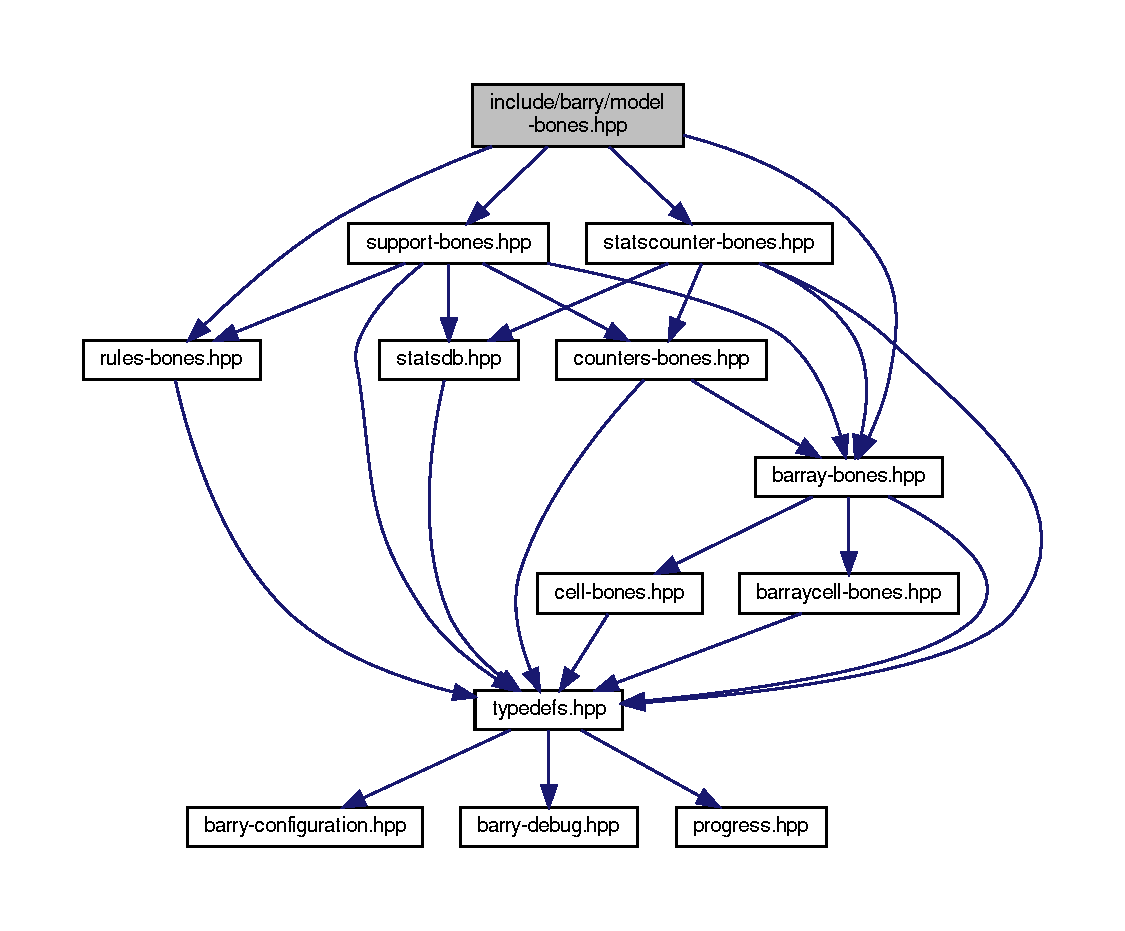
\includegraphics[width=350pt]{model-bones_8hpp__incl}
\end{center}
\end{figure}
This graph shows which files directly or indirectly include this file\+:
\nopagebreak
\begin{figure}[H]
\begin{center}
\leavevmode
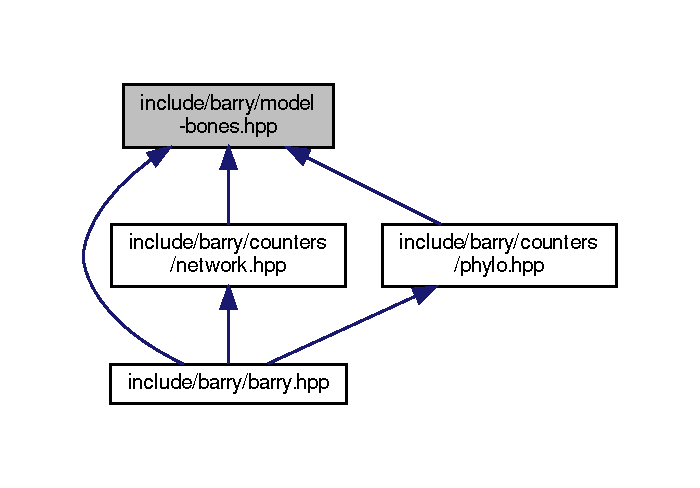
\includegraphics[width=193pt]{model-bones_8hpp__dep__incl}
\end{center}
\end{figure}
\doxysubsection*{Classes}
\begin{DoxyCompactItemize}
\item 
class \mbox{\hyperlink{class_model}{Model$<$ Array\+\_\+\+Type, Data\+\_\+\+Counter\+\_\+\+Type, Data\+\_\+\+Rule\+\_\+\+Type, Data\+\_\+\+Rule\+\_\+\+Dyn\+\_\+\+Type $>$}}
\begin{DoxyCompactList}\small\item\em General framework for discrete exponential models. This class allows generating discrete exponential models in the form of a linear exponential model\+: \end{DoxyCompactList}\end{DoxyCompactItemize}
\doxysubsection*{Functions}
\begin{DoxyCompactItemize}
\item 
{\footnotesize template$<$typename Array\+\_\+\+Type $>$ }\\std\+::vector$<$ double $>$ \mbox{\hyperlink{model-bones_8hpp_ac8a92bc92bfb721602c0470f3efa4f84}{keygen\+\_\+default}} (\mbox{\hyperlink{barraydense-meat_8hpp_a92b303b76a3f942ea819498907d5e83c}{const}} Array\+\_\+\+Type \&\mbox{\hyperlink{barray-meat_8hpp_a6cb31aaad809d508e214b61785d7fb47}{Array\+\_\+}})
\begin{DoxyCompactList}\small\item\em Array Hasher class (used for computing support) \end{DoxyCompactList}\end{DoxyCompactItemize}


\doxysubsection{Function Documentation}
\mbox{\Hypertarget{model-bones_8hpp_ac8a92bc92bfb721602c0470f3efa4f84}\label{model-bones_8hpp_ac8a92bc92bfb721602c0470f3efa4f84}} 
\index{model-\/bones.hpp@{model-\/bones.hpp}!keygen\_default@{keygen\_default}}
\index{keygen\_default@{keygen\_default}!model-\/bones.hpp@{model-\/bones.hpp}}
\doxysubsubsection{\texorpdfstring{keygen\_default()}{keygen\_default()}}
{\footnotesize\ttfamily template$<$typename Array\+\_\+\+Type $>$ \\
std\+::vector$<$ double $>$ keygen\+\_\+default (\begin{DoxyParamCaption}\item[{\mbox{\hyperlink{barraydense-meat_8hpp_a92b303b76a3f942ea819498907d5e83c}{const}} Array\+\_\+\+Type \&}]{Array\+\_\+ }\end{DoxyParamCaption})\hspace{0.3cm}{\ttfamily [inline]}}



Array Hasher class (used for computing support) 



Definition at line 16 of file model-\/bones.\+hpp.


\hypertarget{model-meat_8hpp}{}\doxysection{include/barry/model-\/meat.hpp File Reference}
\label{model-meat_8hpp}\index{include/barry/model-\/meat.hpp@{include/barry/model-\/meat.hpp}}
This graph shows which files directly or indirectly include this file\+:
\nopagebreak
\begin{figure}[H]
\begin{center}
\leavevmode
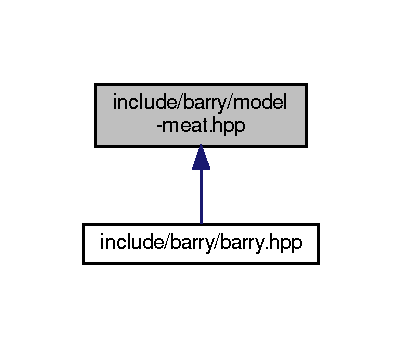
\includegraphics[width=193pt]{model-meat_8hpp__dep__incl}
\end{center}
\end{figure}
\doxysubsection*{Macros}
\begin{DoxyCompactItemize}
\item 
\#define \mbox{\hyperlink{model-meat_8hpp_acc393c765ed15f1e43f163e69da4e06c}{MODEL\+\_\+\+TYPE}}()
\item 
\#define \mbox{\hyperlink{model-meat_8hpp_a9ed2eed6ed65139cb28aabdeffd4c159}{MODEL\+\_\+\+TEMPLATE\+\_\+\+ARGS}}()
\item 
\#define \mbox{\hyperlink{model-meat_8hpp_af3f082842116f298fabd101d2727d773}{MODEL\+\_\+\+TEMPLATE}}(\mbox{\hyperlink{model-meat_8hpp_a0ea8a85723620c90be9fd2a693f12a59}{a}},  b)~    template \mbox{\hyperlink{model-meat_8hpp_a9ed2eed6ed65139cb28aabdeffd4c159}{MODEL\+\_\+\+TEMPLATE\+\_\+\+ARGS}}() inline \mbox{\hyperlink{model-meat_8hpp_a0ea8a85723620c90be9fd2a693f12a59}{a}} \mbox{\hyperlink{model-meat_8hpp_acc393c765ed15f1e43f163e69da4e06c}{MODEL\+\_\+\+TYPE}}()\+::b
\end{DoxyCompactItemize}
\doxysubsection*{Functions}
\begin{DoxyCompactItemize}
\item 
double \mbox{\hyperlink{model-meat_8hpp_a298affefd54bd00274c6af4dd64053be}{update\+\_\+normalizing\+\_\+constant}} (\mbox{\hyperlink{barraydense-meat_8hpp_a92b303b76a3f942ea819498907d5e83c}{const}} double $\ast$\mbox{\hyperlink{model-meat_8hpp_a8b812351f601758974ca8a5020a8f7f2}{params}}, \mbox{\hyperlink{barraydense-meat_8hpp_a92b303b76a3f942ea819498907d5e83c}{const}} double $\ast$support, size\+\_\+t \mbox{\hyperlink{model-meat_8hpp_a9389e4770ba454a2e14f870491495cb2}{k}}, size\+\_\+t n)
\item 
double \mbox{\hyperlink{model-meat_8hpp_a40cd8ec3301c44ffdc24b74e8e4eadc5}{likelihood\+\_\+}} (\mbox{\hyperlink{barraydense-meat_8hpp_a92b303b76a3f942ea819498907d5e83c}{const}} double $\ast$stats\+\_\+target, \mbox{\hyperlink{barraydense-meat_8hpp_a92b303b76a3f942ea819498907d5e83c}{const}} std\+::vector$<$ double $>$ \&\mbox{\hyperlink{model-meat_8hpp_a8b812351f601758974ca8a5020a8f7f2}{params}}, \mbox{\hyperlink{barraydense-meat_8hpp_a92b303b76a3f942ea819498907d5e83c}{const}} double normalizing\+\_\+constant, size\+\_\+t n\+\_\+params, bool log\+\_\+=\mbox{\hyperlink{barraydense-meat_8hpp_ae6c865df784842196d411c1466b01686}{false}})
\item 
\mbox{\hyperlink{model-meat_8hpp_a5fb312eb5849165f1459d10af2a9d1c4}{MODEL\+\_\+\+TEMPLATE}} (void, store\+\_\+psets)() \mbox{\hyperlink{counters-meat_8hpp_ae763aeff9df78ca7be5f904fa4bbdc09}{noexcept}}
\item 
\mbox{\hyperlink{model-meat_8hpp_ac56fba67597d2f9ef96aee188d371615}{MODEL\+\_\+\+TEMPLATE}} (std\+::vector$<$ double $>$, gen\+\_\+key)(\mbox{\hyperlink{barraydense-meat_8hpp_a92b303b76a3f942ea819498907d5e83c}{const}} Array\+\_\+\+Type \&\mbox{\hyperlink{barray-meat_8hpp_a6cb31aaad809d508e214b61785d7fb47}{Array\+\_\+}})
\item 
\mbox{\hyperlink{model-meat_8hpp_ab640e4bcb5db39ca9edfc88c37167b78}{MODEL\+\_\+\+TEMPLATE}} (void, add\+\_\+counter)(\mbox{\hyperlink{class_counter}{Counter}}$<$ Array\+\_\+\+Type
\item 
\mbox{\hyperlink{model-meat_8hpp_add5291bac410eb587280c3df28a23135}{MODEL\+\_\+\+TEMPLATE}} (void, \mbox{\hyperlink{model-meat_8hpp_a891cce5f86ba09c4e4a5202a5f6021b9}{set\+\_\+counters}})(\mbox{\hyperlink{class_counters}{Counters}}$<$ Array\+\_\+\+Type
\item 
support\+\_\+fun \mbox{\hyperlink{model-meat_8hpp_a891cce5f86ba09c4e4a5202a5f6021b9}{set\+\_\+counters}} (\mbox{\hyperlink{support-meat_8hpp_a782c48a908662b34845b6f654f929788}{counters}})
\item 
\mbox{\hyperlink{model-meat_8hpp_a3e4caa6b79e8322bc7438e3b82d88079}{MODEL\+\_\+\+TEMPLATE}} (void, add\+\_\+hasher)(\mbox{\hyperlink{typedefs_8hpp_aab7c9679e747e2f653246fbd03f26cc1}{Hasher\+\_\+fun\+\_\+type}}$<$ Array\+\_\+\+Type
\item 
\mbox{\hyperlink{model-meat_8hpp_a940718c037c10921a73a92d4a086bc8d}{MODEL\+\_\+\+TEMPLATE}} (void, add\+\_\+rule)(\mbox{\hyperlink{class_rule}{Rule}}$<$ Array\+\_\+\+Type
\item 
\mbox{\hyperlink{model-meat_8hpp_a9e51cf15af471cca323b88b48e23c3d9}{MODEL\+\_\+\+TEMPLATE}} (void, \mbox{\hyperlink{model-meat_8hpp_ab636ea2105a33446971af2dc40618a47}{set\+\_\+rules}})(\mbox{\hyperlink{class_rules}{Rules}}$<$ Array\+\_\+\+Type
\item 
support\+\_\+fun \mbox{\hyperlink{model-meat_8hpp_ab636ea2105a33446971af2dc40618a47}{set\+\_\+rules}} (\mbox{\hyperlink{support-meat_8hpp_a595e07a99f60f22a6a29e4fca291ea28}{rules}})
\item 
\mbox{\hyperlink{model-meat_8hpp_af54ed7b85c2a2b246e46bef264889f33}{MODEL\+\_\+\+TEMPLATE}} (void, add\+\_\+rule\+\_\+dyn)(\mbox{\hyperlink{class_rule}{Rule}}$<$ Array\+\_\+\+Type
\item 
\mbox{\hyperlink{model-meat_8hpp_a06c4c06a5261bb7fcf99905b90897091}{MODEL\+\_\+\+TEMPLATE}} (void, \mbox{\hyperlink{model-meat_8hpp_ae09eaba6614a37ca52770bbaf18a876c}{set\+\_\+rules\+\_\+dyn}})(\mbox{\hyperlink{class_rules}{Rules}}$<$ Array\+\_\+\+Type
\item 
support\+\_\+fun \mbox{\hyperlink{model-meat_8hpp_ae09eaba6614a37ca52770bbaf18a876c}{set\+\_\+rules\+\_\+dyn}} (\mbox{\hyperlink{support-meat_8hpp_a2997e52d3d749b34d5a97042e4f520e5}{rules\+\_\+dyn}})
\item 
\mbox{\hyperlink{model-meat_8hpp_a07d08179ab413cc6a09e70b38fc12dff}{MODEL\+\_\+\+TEMPLATE}} (\mbox{\hyperlink{typedefs_8hpp_a91ad9478d81a7aaf2593e8d9c3d06a14}{uint}}, add\+\_\+array)(\mbox{\hyperlink{barraydense-meat_8hpp_a92b303b76a3f942ea819498907d5e83c}{const}} Array\+\_\+\+Type \&\mbox{\hyperlink{barray-meat_8hpp_a6cb31aaad809d508e214b61785d7fb47}{Array\+\_\+}}
\item 
\mbox{\hyperlink{model-meat_8hpp_a95eeb80ec2bed8dfe7cfe4c62f5beee9}{if}} (transform\+\_\+model\+\_\+fun) = transform\+\_\+model\+\_\+fun(\&\mbox{\hyperlink{model-meat_8hpp_a43199108fae59bf79c8d73559aac2cbd}{tmp\+\_\+counts}}\mbox{[}0u\mbox{]}, \mbox{\hyperlink{model-meat_8hpp_a8d73b944a5569bd842f636e4b9d420f6}{tmp\+\_\+counts.\+size}}())
\item 
\mbox{\hyperlink{support-meat_8hpp_a0544c3fe466e421738dae463968b70ba}{else}} stats\+\_\+target \mbox{\hyperlink{model-meat_8hpp_acd4c62abc3c4daf9fb8a68d8e4bd1634}{push\+\_\+back}} (counter\+\_\+fun.\+count\+\_\+all())
\item 
\mbox{\hyperlink{model-meat_8hpp_a6cfd9e26f1cf22d9338dcd14ca5c79ea}{if}} (\mbox{\hyperlink{model-meat_8hpp_a32e3aa42c9a0f6e84cda0c6d011e56f0}{force\+\_\+new}}$\vert$(\mbox{\hyperlink{model-meat_8hpp_a36105d261c658305684678b59d578599}{locator}}==keys2support.\+end()))
\item 
arrays2support \mbox{\hyperlink{model-meat_8hpp_ac76d416dfa2e5dceea5f830850ea25ac}{push\+\_\+back}} (\mbox{\hyperlink{model-meat_8hpp_a36105d261c658305684678b59d578599}{locator}}-\/$>$second)
\item 
\mbox{\hyperlink{model-meat_8hpp_a9ef4985dfa4bd1115422568aac975f7e}{return}} arrays2support \mbox{\hyperlink{model-meat_8hpp_a8d73b944a5569bd842f636e4b9d420f6}{size}} () -\/ 1u
\item 
\mbox{\hyperlink{model-meat_8hpp_a69985c178fd1b57b91edc5dbca8346cc}{MODEL\+\_\+\+TEMPLATE}} (double, likelihood)(\mbox{\hyperlink{barraydense-meat_8hpp_a92b303b76a3f942ea819498907d5e83c}{const}} std
\item 
\mbox{\hyperlink{model-meat_8hpp_a51a39d7d814c7e56a62f339eca277aeb}{MODEL\+\_\+\+TEMPLATE}} (double, likelihood\+\_\+total)(\mbox{\hyperlink{barraydense-meat_8hpp_a92b303b76a3f942ea819498907d5e83c}{const}} std
\item 
\mbox{\hyperlink{model-meat_8hpp_aecfb1a328febc3f5a53fcc5e83e53836}{MODEL\+\_\+\+TEMPLATE}} (double, get\+\_\+norm\+\_\+const)(\mbox{\hyperlink{barraydense-meat_8hpp_a92b303b76a3f942ea819498907d5e83c}{const}} std
\item 
\mbox{\hyperlink{model-meat_8hpp_a4e1c4165f3f8b998efb078d484f39f2f}{MODEL\+\_\+\+TEMPLATE}} (\mbox{\hyperlink{barraydense-meat_8hpp_a92b303b76a3f942ea819498907d5e83c}{const}} std\+::vector$<$ Array\+\_\+\+Type $>$ $\ast$, get\+\_\+pset)(\mbox{\hyperlink{barraydense-meat_8hpp_a92b303b76a3f942ea819498907d5e83c}{const}} \mbox{\hyperlink{typedefs_8hpp_a91ad9478d81a7aaf2593e8d9c3d06a14}{uint}} \&\mbox{\hyperlink{model-meat_8hpp_a5ffdab09665dc9b260b5263cdca94295}{i}})
\item 
\mbox{\hyperlink{model-meat_8hpp_ab21d5328ab0001d3ab8b31a5121daadc}{MODEL\+\_\+\+TEMPLATE}} (\mbox{\hyperlink{barraydense-meat_8hpp_a92b303b76a3f942ea819498907d5e83c}{const}} std\+::vector$<$ double $>$ $\ast$, get\+\_\+pset\+\_\+stats)(\mbox{\hyperlink{barraydense-meat_8hpp_a92b303b76a3f942ea819498907d5e83c}{const}} \mbox{\hyperlink{typedefs_8hpp_a91ad9478d81a7aaf2593e8d9c3d06a14}{uint}} \&\mbox{\hyperlink{model-meat_8hpp_a5ffdab09665dc9b260b5263cdca94295}{i}})
\item 
\mbox{\hyperlink{model-meat_8hpp_a450c500f7d638a6a1182e6a1e2e02cac}{MODEL\+\_\+\+TEMPLATE}} (void, print\+\_\+stats)(\mbox{\hyperlink{typedefs_8hpp_a91ad9478d81a7aaf2593e8d9c3d06a14}{uint}} \mbox{\hyperlink{model-meat_8hpp_a5ffdab09665dc9b260b5263cdca94295}{i}}) \mbox{\hyperlink{barraydense-meat_8hpp_a92b303b76a3f942ea819498907d5e83c}{const}}
\item 
\mbox{\hyperlink{model-meat_8hpp_aac2e854c87c551227c6df8d76bad44fe}{MODEL\+\_\+\+TEMPLATE}} (\mbox{\hyperlink{typedefs_8hpp_a91ad9478d81a7aaf2593e8d9c3d06a14}{uint}}, \mbox{\hyperlink{model-meat_8hpp_a8d73b944a5569bd842f636e4b9d420f6}{size}})() \mbox{\hyperlink{barraydense-meat_8hpp_a92b303b76a3f942ea819498907d5e83c}{const}} \mbox{\hyperlink{counters-meat_8hpp_ae763aeff9df78ca7be5f904fa4bbdc09}{noexcept}}
\item 
\mbox{\hyperlink{model-meat_8hpp_a9f096842d145d26770aae36e718b3f9c}{MODEL\+\_\+\+TEMPLATE}} (\mbox{\hyperlink{typedefs_8hpp_a91ad9478d81a7aaf2593e8d9c3d06a14}{uint}}, size\+\_\+unique)() \mbox{\hyperlink{barraydense-meat_8hpp_a92b303b76a3f942ea819498907d5e83c}{const}} \mbox{\hyperlink{counters-meat_8hpp_ae763aeff9df78ca7be5f904fa4bbdc09}{noexcept}}
\item 
\mbox{\hyperlink{model-meat_8hpp_ab44a1b7b625b818962502b6a0083087c}{MODEL\+\_\+\+TEMPLATE}} (\mbox{\hyperlink{typedefs_8hpp_a91ad9478d81a7aaf2593e8d9c3d06a14}{uint}}, nterms)() \mbox{\hyperlink{barraydense-meat_8hpp_a92b303b76a3f942ea819498907d5e83c}{const}} \mbox{\hyperlink{counters-meat_8hpp_ae763aeff9df78ca7be5f904fa4bbdc09}{noexcept}}
\item 
\mbox{\hyperlink{model-meat_8hpp_a7edcbf23c59017d70906dc693d25b799}{MODEL\+\_\+\+TEMPLATE}} (\mbox{\hyperlink{typedefs_8hpp_a91ad9478d81a7aaf2593e8d9c3d06a14}{uint}}, nrules)() \mbox{\hyperlink{barraydense-meat_8hpp_a92b303b76a3f942ea819498907d5e83c}{const}} \mbox{\hyperlink{counters-meat_8hpp_ae763aeff9df78ca7be5f904fa4bbdc09}{noexcept}}
\item 
\mbox{\hyperlink{model-meat_8hpp_a5100106ddb37b151f073d1d2dc40bf88}{MODEL\+\_\+\+TEMPLATE}} (\mbox{\hyperlink{typedefs_8hpp_a91ad9478d81a7aaf2593e8d9c3d06a14}{uint}}, nrules\+\_\+dyn)() \mbox{\hyperlink{barraydense-meat_8hpp_a92b303b76a3f942ea819498907d5e83c}{const}} \mbox{\hyperlink{counters-meat_8hpp_ae763aeff9df78ca7be5f904fa4bbdc09}{noexcept}}
\item 
\mbox{\hyperlink{model-meat_8hpp_af97749db5f833763b6d09b8c05dbefb6}{MODEL\+\_\+\+TEMPLATE}} (\mbox{\hyperlink{typedefs_8hpp_a91ad9478d81a7aaf2593e8d9c3d06a14}{uint}}, support\+\_\+size)() \mbox{\hyperlink{barraydense-meat_8hpp_a92b303b76a3f942ea819498907d5e83c}{const}} \mbox{\hyperlink{counters-meat_8hpp_ae763aeff9df78ca7be5f904fa4bbdc09}{noexcept}}
\item 
\mbox{\hyperlink{model-meat_8hpp_a3770fd8c8b8d3649a101c80e77cf5092}{MODEL\+\_\+\+TEMPLATE}} (std\+::vector$<$ std\+::string $>$, colnames)() \mbox{\hyperlink{barraydense-meat_8hpp_a92b303b76a3f942ea819498907d5e83c}{const}}
\item 
\mbox{\hyperlink{model-meat_8hpp_a9c6303be0fc1fb92393b587404cb152f}{MODEL\+\_\+\+TEMPLATE}} (Array\+\_\+\+Type, sample)(\mbox{\hyperlink{barraydense-meat_8hpp_a92b303b76a3f942ea819498907d5e83c}{const}} Array\+\_\+\+Type \&\mbox{\hyperlink{barray-meat_8hpp_a6cb31aaad809d508e214b61785d7fb47}{Array\+\_\+}}
\item 
\mbox{\hyperlink{model-meat_8hpp_ae0cc58172b429d3838ce1261ec5d78e4}{if}} (\mbox{\hyperlink{model-meat_8hpp_a36105d261c658305684678b59d578599}{locator}}==keys2support.\+end())
\item 
std\+::uniform\+\_\+real\+\_\+distribution \mbox{\hyperlink{model-meat_8hpp_ac41994c414d968a397a48b933272453f}{urand}} (0, 1)
\item 
\mbox{\hyperlink{model-meat_8hpp_a9d60367e064d8367dc84b5de42870332}{if}} ((\mbox{\hyperlink{model-meat_8hpp_a8d73b944a5569bd842f636e4b9d420f6}{probs.\+size}}() $>$ 0u) \&\&(\mbox{\hyperlink{typedefs_8hpp_aed8ddfe5ae95bf4d6f76221ce06566fb}{vec\+\_\+equal\+\_\+approx}}(\mbox{\hyperlink{model-meat_8hpp_a8b812351f601758974ca8a5020a8f7f2}{params}}, params\+\_\+last\mbox{[}\mbox{\hyperlink{model-meat_8hpp_a0ea8a85723620c90be9fd2a693f12a59}{a}}\mbox{]})))
\item 
std\+::vector$<$ double $>$ \mbox{\hyperlink{model-meat_8hpp_ade0c4a5bb093e62686d62f2dd009bd25}{temp\+\_\+stats}} (\mbox{\hyperlink{model-meat_8hpp_a8d73b944a5569bd842f636e4b9d420f6}{params.\+size}}())
\item 
\mbox{\hyperlink{model-meat_8hpp_a0d7d60577ad0b6507f74f18ab2eccab9}{for}} (size\+\_\+t array=0u;array$<$ \mbox{\hyperlink{model-meat_8hpp_a8d73b944a5569bd842f636e4b9d420f6}{probs.\+size}}();++array)
\item 
\mbox{\hyperlink{model-meat_8hpp_a344cf38d0b829e04052739fcd74e3b8b}{MODEL\+\_\+\+TEMPLATE}} (double, conditional\+\_\+prob)(\mbox{\hyperlink{barraydense-meat_8hpp_a92b303b76a3f942ea819498907d5e83c}{const}} Array\+\_\+\+Type \&\mbox{\hyperlink{barray-meat_8hpp_a6cb31aaad809d508e214b61785d7fb47}{Array\+\_\+}}
\item 
A \mbox{\hyperlink{model-meat_8hpp_a4caf204372c3c29af6d87e56708bdba1}{insert\+\_\+cell}} (\mbox{\hyperlink{model-meat_8hpp_a5ffdab09665dc9b260b5263cdca94295}{i}}, \mbox{\hyperlink{statscounter-meat_8hpp_abbe66f29402555d707260862a10eb56e}{j}}, A.\+default\+\_\+val(), true, \mbox{\hyperlink{barraydense-meat_8hpp_ae6c865df784842196d411c1466b01686}{false}})
\item 
std\+::vector$<$ double $>$ \mbox{\hyperlink{model-meat_8hpp_a43199108fae59bf79c8d73559aac2cbd}{tmp\+\_\+counts}} (\mbox{\hyperlink{support-meat_8hpp_a782c48a908662b34845b6f654f929788}{counters}}-\/$>$\mbox{\hyperlink{model-meat_8hpp_a8d73b944a5569bd842f636e4b9d420f6}{size}}())
\item 
\mbox{\hyperlink{model-meat_8hpp_a9ef4985dfa4bd1115422568aac975f7e}{return}} (1.\+0+std\+::exp(-\/\mbox{\hyperlink{typedefs_8hpp_af6f9c021aa2e49b1cb82fbd32026f1dc}{vec\+\_\+inner\+\_\+prod}}$<$ double $>$(\&\mbox{\hyperlink{model-meat_8hpp_a8b812351f601758974ca8a5020a8f7f2}{params}}\mbox{[}0u\mbox{]}, \&\mbox{\hyperlink{model-meat_8hpp_a43199108fae59bf79c8d73559aac2cbd}{tmp\+\_\+counts}}\mbox{[}0u\mbox{]}, \mbox{\hyperlink{model-meat_8hpp_a8d73b944a5569bd842f636e4b9d420f6}{params.\+size}}())))
\item 
\mbox{\hyperlink{model-meat_8hpp_a1e31bdab44335dab4b1ccc082a624fdd}{MODEL\+\_\+\+TEMPLATE}} (\mbox{\hyperlink{barraydense-meat_8hpp_a92b303b76a3f942ea819498907d5e83c}{const}} std\+::mt19937 $\ast$, get\+\_\+rengine)() \mbox{\hyperlink{barraydense-meat_8hpp_a92b303b76a3f942ea819498907d5e83c}{const}}
\item 
\mbox{\hyperlink{model-meat_8hpp_abdedbda5f86170e660b4bb11c4827887}{MODEL\+\_\+\+TEMPLATE}} (std\+::vector$<$ std\+::vector$<$ double $>$ $>$ $\ast$, get\+\_\+stats\+\_\+target)()
\item 
\mbox{\hyperlink{model-meat_8hpp_a4eee01b8ead8e269f8af5ba2142efa30}{MODEL\+\_\+\+TEMPLATE}} (std\+::vector$<$ std\+::vector$<$ double $>$ $>$ $\ast$, get\+\_\+stats\+\_\+support)()
\item 
\mbox{\hyperlink{model-meat_8hpp_af3ed726d2254547b0c7c030b7ed940f3}{MODEL\+\_\+\+TEMPLATE}} (std\+::vector$<$ unsigned int $>$ $\ast$, get\+\_\+arrays2support)()
\item 
\mbox{\hyperlink{model-meat_8hpp_a1b4ab38ad856016e67ff1975c140089e}{MODEL\+\_\+\+TEMPLATE}} (std\+::vector$<$ std\+::vector$<$ Array\+\_\+\+Type $>$ $>$ $\ast$, get\+\_\+pset\+\_\+arrays)()
\item 
\mbox{\hyperlink{model-meat_8hpp_a05d64a51381043e545359fd19d01d98a}{MODEL\+\_\+\+TEMPLATE}} (std\+::vector$<$ std\+::vector$<$ double $>$ $>$ $\ast$, get\+\_\+pset\+\_\+stats)()
\item 
\mbox{\hyperlink{model-meat_8hpp_a3d6c96b5bf647f75c79ca488d7c9d607}{MODEL\+\_\+\+TEMPLATE}} (std\+::vector$<$ std\+::vector$<$ double $>$ $>$ $\ast$, get\+\_\+pset\+\_\+probs)()
\item 
\mbox{\hyperlink{model-meat_8hpp_ab15b13990207319d7cfdd25be5a04105}{MODEL\+\_\+\+TEMPLATE}} (void, set\+\_\+transform\+\_\+model)(std
\end{DoxyCompactItemize}
\doxysubsection*{Variables}
\begin{DoxyCompactItemize}
\item 
\mbox{\hyperlink{model-meat_8hpp_a69b87f58d3fa400f5d9b076072530f69}{Data\+\_\+\+Counter\+\_\+\+Type}} \& \mbox{\hyperlink{model-meat_8hpp_a7eb7ba1e03825c85183cb90dc0635de4}{counter}}
\item 
\mbox{\hyperlink{model-meat_8hpp_a9717e7bbecb906637e86cef6da3d83c2}{return}}
\item 
\mbox{\hyperlink{model-meat_8hpp_a69b87f58d3fa400f5d9b076072530f69}{Data\+\_\+\+Counter\+\_\+\+Type}} \mbox{\hyperlink{model-meat_8hpp_a2648076475c82f8bfed17e9c46b36f68}{count\+\_\+fun\+\_\+}}
\item 
\mbox{\hyperlink{model-meat_8hpp_a69b87f58d3fa400f5d9b076072530f69}{Data\+\_\+\+Counter\+\_\+\+Type}} \mbox{\hyperlink{typedefs_8hpp_a6a6ce8184bcdbb465486ebb7ca9ec76b}{Counter\+\_\+fun\+\_\+type}}$<$ Array\+\_\+\+Type, \mbox{\hyperlink{model-meat_8hpp_a69b87f58d3fa400f5d9b076072530f69}{Data\+\_\+\+Counter\+\_\+\+Type}} $>$ \mbox{\hyperlink{model-meat_8hpp_aa9ebe808e2d37ce1008f4e98fe5c5c6b}{init\+\_\+fun\+\_\+}}
\item 
\mbox{\hyperlink{model-meat_8hpp_a69b87f58d3fa400f5d9b076072530f69}{Data\+\_\+\+Counter\+\_\+\+Type}} \mbox{\hyperlink{typedefs_8hpp_a6a6ce8184bcdbb465486ebb7ca9ec76b}{Counter\+\_\+fun\+\_\+type}}$<$ Array\+\_\+\+Type, \mbox{\hyperlink{model-meat_8hpp_a69b87f58d3fa400f5d9b076072530f69}{Data\+\_\+\+Counter\+\_\+\+Type}} $>$ \mbox{\hyperlink{model-meat_8hpp_a69b87f58d3fa400f5d9b076072530f69}{Data\+\_\+\+Counter\+\_\+\+Type}} \mbox{\hyperlink{model-meat_8hpp_add877eae455a35aea9e5c7de9c6f2dbb}{data\+\_\+}}
\item 
\mbox{\hyperlink{model-meat_8hpp_a69b87f58d3fa400f5d9b076072530f69}{Data\+\_\+\+Counter\+\_\+\+Type}} $\ast$ \mbox{\hyperlink{model-meat_8hpp_aa79c6fa1f7864a8258e8f2c0a68b6d35}{counters\+\_\+}}
\item 
\mbox{\hyperlink{model-meat_8hpp_a69b87f58d3fa400f5d9b076072530f69}{Data\+\_\+\+Counter\+\_\+\+Type}} \mbox{\hyperlink{model-meat_8hpp_ab8ef6c3e79d05d9438b72a41339d7842}{fun\+\_\+}}
\item 
\mbox{\hyperlink{model-meat_8hpp_ab662732874257647dc631846c67da586}{Data\+\_\+\+Rule\+\_\+\+Type}} \& \mbox{\hyperlink{model-meat_8hpp_a9182438a7dfb477d783232a9256027bb}{rules}}
\item 
\mbox{\hyperlink{model-meat_8hpp_ab662732874257647dc631846c67da586}{Data\+\_\+\+Rule\+\_\+\+Type}} $\ast$ \mbox{\hyperlink{model-meat_8hpp_a193348dc03fb67a29c0fbac36e823588}{rules\+\_\+}}
\item 
\mbox{\hyperlink{barray-meat-operators_8hpp_a16b15c19feaca0a6aa77abb6865710ef}{this}} \mbox{\hyperlink{model-meat_8hpp_aa497331abaad5b5e074d2c8069c82095}{delete\+\_\+rules}} = \mbox{\hyperlink{barraydense-meat_8hpp_ae6c865df784842196d411c1466b01686}{false}}
\item 
Data\+\_\+\+Rule\+\_\+\+Dyn\+\_\+\+Type \mbox{\hyperlink{model-meat_8hpp_ad3d009522a41d83535b5e753b0d8fbf8}{rule\+\_\+fun\+\_\+}}
\item 
\mbox{\hyperlink{barray-meat-operators_8hpp_a16b15c19feaca0a6aa77abb6865710ef}{this}} \mbox{\hyperlink{model-meat_8hpp_aabe2227b11b09aa9567f8e6b282c3f57}{rules\+\_\+dyn}} = \mbox{\hyperlink{support-meat_8hpp_af9e399b166589474207166108d1b93d2}{rules\+\_\+}}
\item 
\mbox{\hyperlink{barray-meat-operators_8hpp_a16b15c19feaca0a6aa77abb6865710ef}{this}} \mbox{\hyperlink{model-meat_8hpp_a8a6558a1649d2586cf34bcbba0b78030}{delete\+\_\+rules\+\_\+dyn}} = \mbox{\hyperlink{barraydense-meat_8hpp_ae6c865df784842196d411c1466b01686}{false}}
\item 
bool \mbox{\hyperlink{model-meat_8hpp_a32e3aa42c9a0f6e84cda0c6d011e56f0}{force\+\_\+new}}
\item 
std\+::vector$<$ double $>$ \mbox{\hyperlink{model-meat_8hpp_af101e9ca6306855e019e0e18f0690468}{key}} = \mbox{\hyperlink{support-meat_8hpp_a782c48a908662b34845b6f654f929788}{counters}}-\/$>$gen\+\_\+hash(\mbox{\hyperlink{barray-meat_8hpp_a6cb31aaad809d508e214b61785d7fb47}{Array\+\_\+}})
\item 
\mbox{\hyperlink{typedefs_8hpp_a02ed8dec96bc528c8bc3d8cb3c4674a5}{Map\+Vec\+\_\+type}}$<$ double, \mbox{\hyperlink{typedefs_8hpp_a91ad9478d81a7aaf2593e8d9c3d06a14}{uint}} $>$\+::const\+\_\+iterator \mbox{\hyperlink{model-meat_8hpp_a36105d261c658305684678b59d578599}{locator}} = keys2support.\+find(\mbox{\hyperlink{model-meat_8hpp_af101e9ca6306855e019e0e18f0690468}{key}})
\item 
\mbox{\hyperlink{model-meat_8hpp_a067bec3fe3db997771ba2ce3868cbda7}{stats\+\_\+support\+\_\+n\+\_\+arrays}} \mbox{[}\mbox{\hyperlink{model-meat_8hpp_a36105d261c658305684678b59d578599}{locator}}-\/$>$second\mbox{]}
\item 
\mbox{\hyperlink{barraydense-meat_8hpp_a92b303b76a3f942ea819498907d5e83c}{const}} std\+::vector$<$ double $>$ \& \mbox{\hyperlink{model-meat_8hpp_a8b812351f601758974ca8a5020a8f7f2}{params}}
\item 
size\+\_\+t \mbox{\hyperlink{model-meat_8hpp_a5ffdab09665dc9b260b5263cdca94295}{i}} = \mbox{\hyperlink{model-meat_8hpp_a36105d261c658305684678b59d578599}{locator}}-\/$>$second
\item 
unsigned int \mbox{\hyperlink{model-meat_8hpp_a0ea8a85723620c90be9fd2a693f12a59}{a}} = arrays2support\mbox{[}\mbox{\hyperlink{model-meat_8hpp_a5ffdab09665dc9b260b5263cdca94295}{i}}\mbox{]}
\item 
double \mbox{\hyperlink{model-meat_8hpp_a880a49112fedae68e714341a9a082fb6}{r}} = \mbox{\hyperlink{model-meat_8hpp_ac41994c414d968a397a48b933272453f}{urand}}($\ast$rengine)
\item 
double \mbox{\hyperlink{model-meat_8hpp_aeea68eecbfe5f35e520ebf20c508dd10}{cumprob}} = 0.\+0
\item 
size\+\_\+t \mbox{\hyperlink{model-meat_8hpp_a9389e4770ba454a2e14f870491495cb2}{k}} = \mbox{\hyperlink{model-meat_8hpp_a8d73b944a5569bd842f636e4b9d420f6}{params.\+size}}()
\item 
unsigned int \mbox{\hyperlink{model-meat_8hpp_a36e925890a44a3f7c7c77e867468ecac}{j}} = 0u
\item 
std\+::vector$<$ double $>$ \& \mbox{\hyperlink{model-meat_8hpp_ab14bb4f5b80bcefa0fc098e58e5b44f6}{probs}} = pset\+\_\+probs\mbox{[}\mbox{\hyperlink{model-meat_8hpp_a0ea8a85723620c90be9fd2a693f12a59}{a}}\mbox{]}
\item 
\mbox{\hyperlink{model-meat_8hpp_a0544c3fe466e421738dae463968b70ba}{else}}
\item 
\mbox{\hyperlink{barraydense-meat_8hpp_a92b303b76a3f942ea819498907d5e83c}{const}} std\+::vector$<$ double $>$ \& \mbox{\hyperlink{model-meat_8hpp_ada7a2adf3edef6b8859ce756bd31e4b6}{stats}} = pset\+\_\+stats\mbox{[}\mbox{\hyperlink{model-meat_8hpp_a0ea8a85723620c90be9fd2a693f12a59}{a}}\mbox{]}
\item 
int \mbox{\hyperlink{model-meat_8hpp_a091414baaf8fc6076ca08c2c0ede7066}{i\+\_\+matches}} = -\/1
\item 
\mbox{\hyperlink{model-meat_8hpp_a9ef4985dfa4bd1115422568aac975f7e}{return}} \mbox{\hyperlink{barray-meat-operators_8hpp_a16b15c19feaca0a6aa77abb6865710ef}{this}} \mbox{\hyperlink{model-meat_8hpp_adb446932e2140e5a8c0420d63fe1300e}{pset\+\_\+arrays}} \mbox{[}\mbox{\hyperlink{model-meat_8hpp_a0ea8a85723620c90be9fd2a693f12a59}{a}}\mbox{]}\mbox{[}\mbox{\hyperlink{statscounter-meat_8hpp_abbe66f29402555d707260862a10eb56e}{j}}\mbox{]}
\item 
template \mbox{\hyperlink{model-meat_8hpp_a69b87f58d3fa400f5d9b076072530f69}{Data\+\_\+\+Counter\+\_\+\+Type}}
\item 
template \mbox{\hyperlink{model-meat_8hpp_ab662732874257647dc631846c67da586}{Data\+\_\+\+Rule\+\_\+\+Type}}
\end{DoxyCompactItemize}


\doxysubsection{Macro Definition Documentation}
\mbox{\Hypertarget{model-meat_8hpp_af3f082842116f298fabd101d2727d773}\label{model-meat_8hpp_af3f082842116f298fabd101d2727d773}} 
\index{model-\/meat.hpp@{model-\/meat.hpp}!MODEL\_TEMPLATE@{MODEL\_TEMPLATE}}
\index{MODEL\_TEMPLATE@{MODEL\_TEMPLATE}!model-\/meat.hpp@{model-\/meat.hpp}}
\doxysubsubsection{\texorpdfstring{MODEL\_TEMPLATE}{MODEL\_TEMPLATE}}
{\footnotesize\ttfamily \#define MODEL\+\_\+\+TEMPLATE(\begin{DoxyParamCaption}\item[{}]{\mbox{\hyperlink{model-meat_8hpp_a0ea8a85723620c90be9fd2a693f12a59}{a}},  }\item[{}]{b }\end{DoxyParamCaption})~    template \mbox{\hyperlink{model-meat_8hpp_a9ed2eed6ed65139cb28aabdeffd4c159}{MODEL\+\_\+\+TEMPLATE\+\_\+\+ARGS}}() inline \mbox{\hyperlink{model-meat_8hpp_a0ea8a85723620c90be9fd2a693f12a59}{a}} \mbox{\hyperlink{model-meat_8hpp_acc393c765ed15f1e43f163e69da4e06c}{MODEL\+\_\+\+TYPE}}()\+::b}



Definition at line 87 of file model-\/meat.\+hpp.

\mbox{\Hypertarget{model-meat_8hpp_a9ed2eed6ed65139cb28aabdeffd4c159}\label{model-meat_8hpp_a9ed2eed6ed65139cb28aabdeffd4c159}} 
\index{model-\/meat.hpp@{model-\/meat.hpp}!MODEL\_TEMPLATE\_ARGS@{MODEL\_TEMPLATE\_ARGS}}
\index{MODEL\_TEMPLATE\_ARGS@{MODEL\_TEMPLATE\_ARGS}!model-\/meat.hpp@{model-\/meat.hpp}}
\doxysubsubsection{\texorpdfstring{MODEL\_TEMPLATE\_ARGS}{MODEL\_TEMPLATE\_ARGS}}
{\footnotesize\ttfamily template MODEL\+\_\+\+TEMPLATE\+\_\+\+ARGS(\begin{DoxyParamCaption}{ }\end{DoxyParamCaption})}

{\bfseries Value\+:}
\begin{DoxyCode}{0}
\DoxyCodeLine{    <\textcolor{keyword}{typename} Array\_Type, \textcolor{keyword}{typename} \mbox{\hyperlink{model-meat_8hpp_a69b87f58d3fa400f5d9b076072530f69}{Data\_Counter\_Type}},\(\backslash\)}
\DoxyCodeLine{    typename \mbox{\hyperlink{model-meat_8hpp_ab662732874257647dc631846c67da586}{Data\_Rule\_Type}}, \textcolor{keyword}{typename} Data\_Rule\_Dyn\_Type>}

\end{DoxyCode}


Definition at line 84 of file model-\/meat.\+hpp.

\mbox{\Hypertarget{model-meat_8hpp_acc393c765ed15f1e43f163e69da4e06c}\label{model-meat_8hpp_acc393c765ed15f1e43f163e69da4e06c}} 
\index{model-\/meat.hpp@{model-\/meat.hpp}!MODEL\_TYPE@{MODEL\_TYPE}}
\index{MODEL\_TYPE@{MODEL\_TYPE}!model-\/meat.hpp@{model-\/meat.hpp}}
\doxysubsubsection{\texorpdfstring{MODEL\_TYPE}{MODEL\_TYPE}}
{\footnotesize\ttfamily template Data\+\_\+\+Rule\+\_\+\+Dyn\+\_\+\+Type $\ast$ MODEL\+\_\+\+TYPE(\begin{DoxyParamCaption}{ }\end{DoxyParamCaption})}

{\bfseries Value\+:}
\begin{DoxyCode}{0}
\DoxyCodeLine{    \mbox{\hyperlink{class_model}{Model}}<Array\_Type,\mbox{\hyperlink{model-meat_8hpp_a69b87f58d3fa400f5d9b076072530f69}{Data\_Counter\_Type}},\mbox{\hyperlink{model-meat_8hpp_ab662732874257647dc631846c67da586}{Data\_Rule\_Type}},\(\backslash\)}
\DoxyCodeLine{    Data\_Rule\_Dyn\_Type>}

\end{DoxyCode}


Definition at line 81 of file model-\/meat.\+hpp.



\doxysubsection{Function Documentation}
\mbox{\Hypertarget{model-meat_8hpp_a0d7d60577ad0b6507f74f18ab2eccab9}\label{model-meat_8hpp_a0d7d60577ad0b6507f74f18ab2eccab9}} 
\index{model-\/meat.hpp@{model-\/meat.hpp}!for@{for}}
\index{for@{for}!model-\/meat.hpp@{model-\/meat.hpp}}
\doxysubsubsection{\texorpdfstring{for()}{for()}}
{\footnotesize\ttfamily for (\begin{DoxyParamCaption}{ }\end{DoxyParamCaption})}



Definition at line 1234 of file model-\/meat.\+hpp.

\mbox{\Hypertarget{model-meat_8hpp_a9d60367e064d8367dc84b5de42870332}\label{model-meat_8hpp_a9d60367e064d8367dc84b5de42870332}} 
\index{model-\/meat.hpp@{model-\/meat.hpp}!if@{if}}
\index{if@{if}!model-\/meat.hpp@{model-\/meat.hpp}}
\doxysubsubsection{\texorpdfstring{if()}{if()}\hspace{0.1cm}{\footnotesize\ttfamily [1/4]}}
{\footnotesize\ttfamily if (\begin{DoxyParamCaption}\item[{(\mbox{\hyperlink{model-meat_8hpp_a8d73b944a5569bd842f636e4b9d420f6}{probs.\+size}}() $>$ 0u) \&\&(\mbox{\hyperlink{typedefs_8hpp_aed8ddfe5ae95bf4d6f76221ce06566fb}{vec\+\_\+equal\+\_\+approx}}(\mbox{\hyperlink{model-meat_8hpp_a8b812351f601758974ca8a5020a8f7f2}{params}}, params\+\_\+last\mbox{[}\mbox{\hyperlink{model-meat_8hpp_a0ea8a85723620c90be9fd2a693f12a59}{a}}\mbox{]}))}]{ }\end{DoxyParamCaption})}



Definition at line 1218 of file model-\/meat.\+hpp.

\mbox{\Hypertarget{model-meat_8hpp_a6cfd9e26f1cf22d9338dcd14ca5c79ea}\label{model-meat_8hpp_a6cfd9e26f1cf22d9338dcd14ca5c79ea}} 
\index{model-\/meat.hpp@{model-\/meat.hpp}!if@{if}}
\index{if@{if}!model-\/meat.hpp@{model-\/meat.hpp}}
\doxysubsubsection{\texorpdfstring{if()}{if()}\hspace{0.1cm}{\footnotesize\ttfamily [2/4]}}
{\footnotesize\ttfamily if (\begin{DoxyParamCaption}\item[{\mbox{\hyperlink{model-meat_8hpp_a32e3aa42c9a0f6e84cda0c6d011e56f0}{force\+\_\+new}}$\vert$}]{locator==keys2support.\+end() }\end{DoxyParamCaption})}

When computing with the powerset, we need to grow the corresponding vectors on the fly

Definition at line 409 of file model-\/meat.\+hpp.

\mbox{\Hypertarget{model-meat_8hpp_ae0cc58172b429d3838ce1261ec5d78e4}\label{model-meat_8hpp_ae0cc58172b429d3838ce1261ec5d78e4}} 
\index{model-\/meat.hpp@{model-\/meat.hpp}!if@{if}}
\index{if@{if}!model-\/meat.hpp@{model-\/meat.hpp}}
\doxysubsubsection{\texorpdfstring{if()}{if()}\hspace{0.1cm}{\footnotesize\ttfamily [3/4]}}
{\footnotesize\ttfamily if (\begin{DoxyParamCaption}\item[{\mbox{\hyperlink{model-meat_8hpp_a36105d261c658305684678b59d578599}{locator}}}]{ = {\ttfamily =~keys2support.end()} }\end{DoxyParamCaption})}

When computing with the powerset, we need to grow the corresponding vectors on the fly

Definition at line 1120 of file model-\/meat.\+hpp.

\mbox{\Hypertarget{model-meat_8hpp_a95eeb80ec2bed8dfe7cfe4c62f5beee9}\label{model-meat_8hpp_a95eeb80ec2bed8dfe7cfe4c62f5beee9}} 
\index{model-\/meat.hpp@{model-\/meat.hpp}!if@{if}}
\index{if@{if}!model-\/meat.hpp@{model-\/meat.hpp}}
\doxysubsubsection{\texorpdfstring{if()}{if()}\hspace{0.1cm}{\footnotesize\ttfamily [4/4]}}
{\footnotesize\ttfamily if (\begin{DoxyParamCaption}\item[{transform\+\_\+model\+\_\+fun}]{ }\end{DoxyParamCaption}) = transform\+\_\+model\+\_\+fun(\&\mbox{\hyperlink{model-meat_8hpp_a43199108fae59bf79c8d73559aac2cbd}{tmp\+\_\+counts}}\mbox{[}0u\mbox{]}, \mbox{\hyperlink{model-meat_8hpp_a8d73b944a5569bd842f636e4b9d420f6}{tmp\+\_\+counts.\+size}}())}



Definition at line 398 of file model-\/meat.\+hpp.

\mbox{\Hypertarget{model-meat_8hpp_a4caf204372c3c29af6d87e56708bdba1}\label{model-meat_8hpp_a4caf204372c3c29af6d87e56708bdba1}} 
\index{model-\/meat.hpp@{model-\/meat.hpp}!insert\_cell@{insert\_cell}}
\index{insert\_cell@{insert\_cell}!model-\/meat.hpp@{model-\/meat.hpp}}
\doxysubsubsection{\texorpdfstring{insert\_cell()}{insert\_cell()}}
{\footnotesize\ttfamily A insert\+\_\+cell (\begin{DoxyParamCaption}\item[{\mbox{\hyperlink{model-meat_8hpp_a5ffdab09665dc9b260b5263cdca94295}{i}}}]{,  }\item[{\mbox{\hyperlink{statscounter-meat_8hpp_abbe66f29402555d707260862a10eb56e}{j}}}]{,  }\item[{A.}]{default\+\_\+val(),  }\item[{true}]{,  }\item[{\mbox{\hyperlink{barraydense-meat_8hpp_ae6c865df784842196d411c1466b01686}{false}}}]{ }\end{DoxyParamCaption})}

\mbox{\Hypertarget{model-meat_8hpp_a40cd8ec3301c44ffdc24b74e8e4eadc5}\label{model-meat_8hpp_a40cd8ec3301c44ffdc24b74e8e4eadc5}} 
\index{model-\/meat.hpp@{model-\/meat.hpp}!likelihood\_@{likelihood\_}}
\index{likelihood\_@{likelihood\_}!model-\/meat.hpp@{model-\/meat.hpp}}
\doxysubsubsection{\texorpdfstring{likelihood\_()}{likelihood\_()}}
{\footnotesize\ttfamily double likelihood\+\_\+ (\begin{DoxyParamCaption}\item[{\mbox{\hyperlink{barraydense-meat_8hpp_a92b303b76a3f942ea819498907d5e83c}{const}} double $\ast$}]{stats\+\_\+target,  }\item[{\mbox{\hyperlink{barraydense-meat_8hpp_a92b303b76a3f942ea819498907d5e83c}{const}} std\+::vector$<$ double $>$ \&}]{params,  }\item[{\mbox{\hyperlink{barraydense-meat_8hpp_a92b303b76a3f942ea819498907d5e83c}{const}} double}]{normalizing\+\_\+constant,  }\item[{size\+\_\+t}]{n\+\_\+params,  }\item[{bool}]{log\+\_\+ = {\ttfamily \mbox{\hyperlink{barraydense-meat_8hpp_ae6c865df784842196d411c1466b01686}{false}}} }\end{DoxyParamCaption})\hspace{0.3cm}{\ttfamily [inline]}}



Definition at line 45 of file model-\/meat.\+hpp.

\mbox{\Hypertarget{model-meat_8hpp_a9c6303be0fc1fb92393b587404cb152f}\label{model-meat_8hpp_a9c6303be0fc1fb92393b587404cb152f}} 
\index{model-\/meat.hpp@{model-\/meat.hpp}!MODEL\_TEMPLATE@{MODEL\_TEMPLATE}}
\index{MODEL\_TEMPLATE@{MODEL\_TEMPLATE}!model-\/meat.hpp@{model-\/meat.hpp}}
\doxysubsubsection{\texorpdfstring{MODEL\_TEMPLATE()}{MODEL\_TEMPLATE()}\hspace{0.1cm}{\footnotesize\ttfamily [1/33]}}
{\footnotesize\ttfamily MODEL\+\_\+\+TEMPLATE (\begin{DoxyParamCaption}\item[{Array\+\_\+\+Type}]{,  }\item[{sample}]{ }\end{DoxyParamCaption}) const \&}

\mbox{\Hypertarget{model-meat_8hpp_a1e31bdab44335dab4b1ccc082a624fdd}\label{model-meat_8hpp_a1e31bdab44335dab4b1ccc082a624fdd}} 
\index{model-\/meat.hpp@{model-\/meat.hpp}!MODEL\_TEMPLATE@{MODEL\_TEMPLATE}}
\index{MODEL\_TEMPLATE@{MODEL\_TEMPLATE}!model-\/meat.hpp@{model-\/meat.hpp}}
\doxysubsubsection{\texorpdfstring{MODEL\_TEMPLATE()}{MODEL\_TEMPLATE()}\hspace{0.1cm}{\footnotesize\ttfamily [2/33]}}
{\footnotesize\ttfamily MODEL\+\_\+\+TEMPLATE (\begin{DoxyParamCaption}\item[{\mbox{\hyperlink{barraydense-meat_8hpp_a92b303b76a3f942ea819498907d5e83c}{const}} std\+::mt19937 $\ast$}]{,  }\item[{get\+\_\+rengine}]{ }\end{DoxyParamCaption}) const}



Definition at line 1288 of file model-\/meat.\+hpp.

\mbox{\Hypertarget{model-meat_8hpp_a4e1c4165f3f8b998efb078d484f39f2f}\label{model-meat_8hpp_a4e1c4165f3f8b998efb078d484f39f2f}} 
\index{model-\/meat.hpp@{model-\/meat.hpp}!MODEL\_TEMPLATE@{MODEL\_TEMPLATE}}
\index{MODEL\_TEMPLATE@{MODEL\_TEMPLATE}!model-\/meat.hpp@{model-\/meat.hpp}}
\doxysubsubsection{\texorpdfstring{MODEL\_TEMPLATE()}{MODEL\_TEMPLATE()}\hspace{0.1cm}{\footnotesize\ttfamily [3/33]}}
{\footnotesize\ttfamily MODEL\+\_\+\+TEMPLATE (\begin{DoxyParamCaption}\item[{\mbox{\hyperlink{barraydense-meat_8hpp_a92b303b76a3f942ea819498907d5e83c}{const}} std\+::vector$<$ Array\+\_\+\+Type $>$ $\ast$}]{,  }\item[{get\+\_\+pset}]{ }\end{DoxyParamCaption}) const \&}



Definition at line 861 of file model-\/meat.\+hpp.

\mbox{\Hypertarget{model-meat_8hpp_ab21d5328ab0001d3ab8b31a5121daadc}\label{model-meat_8hpp_ab21d5328ab0001d3ab8b31a5121daadc}} 
\index{model-\/meat.hpp@{model-\/meat.hpp}!MODEL\_TEMPLATE@{MODEL\_TEMPLATE}}
\index{MODEL\_TEMPLATE@{MODEL\_TEMPLATE}!model-\/meat.hpp@{model-\/meat.hpp}}
\doxysubsubsection{\texorpdfstring{MODEL\_TEMPLATE()}{MODEL\_TEMPLATE()}\hspace{0.1cm}{\footnotesize\ttfamily [4/33]}}
{\footnotesize\ttfamily MODEL\+\_\+\+TEMPLATE (\begin{DoxyParamCaption}\item[{\mbox{\hyperlink{barraydense-meat_8hpp_a92b303b76a3f942ea819498907d5e83c}{const}} std\+::vector$<$ double $>$ $\ast$}]{,  }\item[{get\+\_\+pset\+\_\+stats}]{ }\end{DoxyParamCaption}) const \&}



Definition at line 873 of file model-\/meat.\+hpp.

\mbox{\Hypertarget{model-meat_8hpp_a344cf38d0b829e04052739fcd74e3b8b}\label{model-meat_8hpp_a344cf38d0b829e04052739fcd74e3b8b}} 
\index{model-\/meat.hpp@{model-\/meat.hpp}!MODEL\_TEMPLATE@{MODEL\_TEMPLATE}}
\index{MODEL\_TEMPLATE@{MODEL\_TEMPLATE}!model-\/meat.hpp@{model-\/meat.hpp}}
\doxysubsubsection{\texorpdfstring{MODEL\_TEMPLATE()}{MODEL\_TEMPLATE()}\hspace{0.1cm}{\footnotesize\ttfamily [5/33]}}
{\footnotesize\ttfamily MODEL\+\_\+\+TEMPLATE (\begin{DoxyParamCaption}\item[{double}]{,  }\item[{conditional\+\_\+prob}]{ }\end{DoxyParamCaption}) const \&}

\mbox{\Hypertarget{model-meat_8hpp_aecfb1a328febc3f5a53fcc5e83e53836}\label{model-meat_8hpp_aecfb1a328febc3f5a53fcc5e83e53836}} 
\index{model-\/meat.hpp@{model-\/meat.hpp}!MODEL\_TEMPLATE@{MODEL\_TEMPLATE}}
\index{MODEL\_TEMPLATE@{MODEL\_TEMPLATE}!model-\/meat.hpp@{model-\/meat.hpp}}
\doxysubsubsection{\texorpdfstring{MODEL\_TEMPLATE()}{MODEL\_TEMPLATE()}\hspace{0.1cm}{\footnotesize\ttfamily [6/33]}}
{\footnotesize\ttfamily MODEL\+\_\+\+TEMPLATE (\begin{DoxyParamCaption}\item[{double}]{,  }\item[{get\+\_\+norm\+\_\+const}]{ }\end{DoxyParamCaption}) const}



Definition at line 825 of file model-\/meat.\+hpp.

\mbox{\Hypertarget{model-meat_8hpp_a69985c178fd1b57b91edc5dbca8346cc}\label{model-meat_8hpp_a69985c178fd1b57b91edc5dbca8346cc}} 
\index{model-\/meat.hpp@{model-\/meat.hpp}!MODEL\_TEMPLATE@{MODEL\_TEMPLATE}}
\index{MODEL\_TEMPLATE@{MODEL\_TEMPLATE}!model-\/meat.hpp@{model-\/meat.hpp}}
\doxysubsubsection{\texorpdfstring{MODEL\_TEMPLATE()}{MODEL\_TEMPLATE()}\hspace{0.1cm}{\footnotesize\ttfamily [7/33]}}
{\footnotesize\ttfamily MODEL\+\_\+\+TEMPLATE (\begin{DoxyParamCaption}\item[{double}]{,  }\item[{likelihood}]{ }\end{DoxyParamCaption}) const}



Definition at line 521 of file model-\/meat.\+hpp.

\mbox{\Hypertarget{model-meat_8hpp_a51a39d7d814c7e56a62f339eca277aeb}\label{model-meat_8hpp_a51a39d7d814c7e56a62f339eca277aeb}} 
\index{model-\/meat.hpp@{model-\/meat.hpp}!MODEL\_TEMPLATE@{MODEL\_TEMPLATE}}
\index{MODEL\_TEMPLATE@{MODEL\_TEMPLATE}!model-\/meat.hpp@{model-\/meat.hpp}}
\doxysubsubsection{\texorpdfstring{MODEL\_TEMPLATE()}{MODEL\_TEMPLATE()}\hspace{0.1cm}{\footnotesize\ttfamily [8/33]}}
{\footnotesize\ttfamily MODEL\+\_\+\+TEMPLATE (\begin{DoxyParamCaption}\item[{double}]{,  }\item[{likelihood\+\_\+total}]{ }\end{DoxyParamCaption}) const}



Definition at line 755 of file model-\/meat.\+hpp.

\mbox{\Hypertarget{model-meat_8hpp_ac56fba67597d2f9ef96aee188d371615}\label{model-meat_8hpp_ac56fba67597d2f9ef96aee188d371615}} 
\index{model-\/meat.hpp@{model-\/meat.hpp}!MODEL\_TEMPLATE@{MODEL\_TEMPLATE}}
\index{MODEL\_TEMPLATE@{MODEL\_TEMPLATE}!model-\/meat.hpp@{model-\/meat.hpp}}
\doxysubsubsection{\texorpdfstring{MODEL\_TEMPLATE()}{MODEL\_TEMPLATE()}\hspace{0.1cm}{\footnotesize\ttfamily [9/33]}}
{\footnotesize\ttfamily MODEL\+\_\+\+TEMPLATE (\begin{DoxyParamCaption}\item[{std\+::vector$<$ double $>$}]{,  }\item[{gen\+\_\+key}]{ }\end{DoxyParamCaption}) const \&}



Definition at line 268 of file model-\/meat.\+hpp.

\mbox{\Hypertarget{model-meat_8hpp_a3770fd8c8b8d3649a101c80e77cf5092}\label{model-meat_8hpp_a3770fd8c8b8d3649a101c80e77cf5092}} 
\index{model-\/meat.hpp@{model-\/meat.hpp}!MODEL\_TEMPLATE@{MODEL\_TEMPLATE}}
\index{MODEL\_TEMPLATE@{MODEL\_TEMPLATE}!model-\/meat.hpp@{model-\/meat.hpp}}
\doxysubsubsection{\texorpdfstring{MODEL\_TEMPLATE()}{MODEL\_TEMPLATE()}\hspace{0.1cm}{\footnotesize\ttfamily [10/33]}}
{\footnotesize\ttfamily MODEL\+\_\+\+TEMPLATE (\begin{DoxyParamCaption}\item[{std\+::vector$<$ std\+::string $>$}]{,  }\item[{colnames}]{ }\end{DoxyParamCaption}) const}



Definition at line 1025 of file model-\/meat.\+hpp.

\mbox{\Hypertarget{model-meat_8hpp_a1b4ab38ad856016e67ff1975c140089e}\label{model-meat_8hpp_a1b4ab38ad856016e67ff1975c140089e}} 
\index{model-\/meat.hpp@{model-\/meat.hpp}!MODEL\_TEMPLATE@{MODEL\_TEMPLATE}}
\index{MODEL\_TEMPLATE@{MODEL\_TEMPLATE}!model-\/meat.hpp@{model-\/meat.hpp}}
\doxysubsubsection{\texorpdfstring{MODEL\_TEMPLATE()}{MODEL\_TEMPLATE()}\hspace{0.1cm}{\footnotesize\ttfamily [11/33]}}
{\footnotesize\ttfamily MODEL\+\_\+\+TEMPLATE (\begin{DoxyParamCaption}\item[{std\+::vector$<$ std\+::vector$<$ Array\+\_\+\+Type $>$ $>$ $\ast$}]{,  }\item[{get\+\_\+pset\+\_\+arrays}]{ }\end{DoxyParamCaption})}



Definition at line 1328 of file model-\/meat.\+hpp.

\mbox{\Hypertarget{model-meat_8hpp_a3d6c96b5bf647f75c79ca488d7c9d607}\label{model-meat_8hpp_a3d6c96b5bf647f75c79ca488d7c9d607}} 
\index{model-\/meat.hpp@{model-\/meat.hpp}!MODEL\_TEMPLATE@{MODEL\_TEMPLATE}}
\index{MODEL\_TEMPLATE@{MODEL\_TEMPLATE}!model-\/meat.hpp@{model-\/meat.hpp}}
\doxysubsubsection{\texorpdfstring{MODEL\_TEMPLATE()}{MODEL\_TEMPLATE()}\hspace{0.1cm}{\footnotesize\ttfamily [12/33]}}
{\footnotesize\ttfamily MODEL\+\_\+\+TEMPLATE (\begin{DoxyParamCaption}\item[{std\+::vector$<$ std\+::vector$<$ double $>$ $>$ $\ast$}]{,  }\item[{get\+\_\+pset\+\_\+probs}]{ }\end{DoxyParamCaption})}



Definition at line 1336 of file model-\/meat.\+hpp.

\mbox{\Hypertarget{model-meat_8hpp_a05d64a51381043e545359fd19d01d98a}\label{model-meat_8hpp_a05d64a51381043e545359fd19d01d98a}} 
\index{model-\/meat.hpp@{model-\/meat.hpp}!MODEL\_TEMPLATE@{MODEL\_TEMPLATE}}
\index{MODEL\_TEMPLATE@{MODEL\_TEMPLATE}!model-\/meat.hpp@{model-\/meat.hpp}}
\doxysubsubsection{\texorpdfstring{MODEL\_TEMPLATE()}{MODEL\_TEMPLATE()}\hspace{0.1cm}{\footnotesize\ttfamily [13/33]}}
{\footnotesize\ttfamily MODEL\+\_\+\+TEMPLATE (\begin{DoxyParamCaption}\item[{std\+::vector$<$ std\+::vector$<$ double $>$ $>$ $\ast$}]{,  }\item[{get\+\_\+pset\+\_\+stats}]{ }\end{DoxyParamCaption})}



Definition at line 1332 of file model-\/meat.\+hpp.

\mbox{\Hypertarget{model-meat_8hpp_a4eee01b8ead8e269f8af5ba2142efa30}\label{model-meat_8hpp_a4eee01b8ead8e269f8af5ba2142efa30}} 
\index{model-\/meat.hpp@{model-\/meat.hpp}!MODEL\_TEMPLATE@{MODEL\_TEMPLATE}}
\index{MODEL\_TEMPLATE@{MODEL\_TEMPLATE}!model-\/meat.hpp@{model-\/meat.hpp}}
\doxysubsubsection{\texorpdfstring{MODEL\_TEMPLATE()}{MODEL\_TEMPLATE()}\hspace{0.1cm}{\footnotesize\ttfamily [14/33]}}
{\footnotesize\ttfamily MODEL\+\_\+\+TEMPLATE (\begin{DoxyParamCaption}\item[{std\+::vector$<$ std\+::vector$<$ double $>$ $>$ $\ast$}]{,  }\item[{get\+\_\+stats\+\_\+support}]{ }\end{DoxyParamCaption})}



Definition at line 1318 of file model-\/meat.\+hpp.

\mbox{\Hypertarget{model-meat_8hpp_abdedbda5f86170e660b4bb11c4827887}\label{model-meat_8hpp_abdedbda5f86170e660b4bb11c4827887}} 
\index{model-\/meat.hpp@{model-\/meat.hpp}!MODEL\_TEMPLATE@{MODEL\_TEMPLATE}}
\index{MODEL\_TEMPLATE@{MODEL\_TEMPLATE}!model-\/meat.hpp@{model-\/meat.hpp}}
\doxysubsubsection{\texorpdfstring{MODEL\_TEMPLATE()}{MODEL\_TEMPLATE()}\hspace{0.1cm}{\footnotesize\ttfamily [15/33]}}
{\footnotesize\ttfamily MODEL\+\_\+\+TEMPLATE (\begin{DoxyParamCaption}\item[{std\+::vector$<$ std\+::vector$<$ double $>$ $>$ $\ast$}]{,  }\item[{get\+\_\+stats\+\_\+target}]{ }\end{DoxyParamCaption})}



Definition at line 1313 of file model-\/meat.\+hpp.

\mbox{\Hypertarget{model-meat_8hpp_af3ed726d2254547b0c7c030b7ed940f3}\label{model-meat_8hpp_af3ed726d2254547b0c7c030b7ed940f3}} 
\index{model-\/meat.hpp@{model-\/meat.hpp}!MODEL\_TEMPLATE@{MODEL\_TEMPLATE}}
\index{MODEL\_TEMPLATE@{MODEL\_TEMPLATE}!model-\/meat.hpp@{model-\/meat.hpp}}
\doxysubsubsection{\texorpdfstring{MODEL\_TEMPLATE()}{MODEL\_TEMPLATE()}\hspace{0.1cm}{\footnotesize\ttfamily [16/33]}}
{\footnotesize\ttfamily MODEL\+\_\+\+TEMPLATE (\begin{DoxyParamCaption}\item[{std\+::vector$<$ unsigned int $>$ $\ast$}]{,  }\item[{get\+\_\+arrays2support}]{ }\end{DoxyParamCaption})}



Definition at line 1323 of file model-\/meat.\+hpp.

\mbox{\Hypertarget{model-meat_8hpp_a07d08179ab413cc6a09e70b38fc12dff}\label{model-meat_8hpp_a07d08179ab413cc6a09e70b38fc12dff}} 
\index{model-\/meat.hpp@{model-\/meat.hpp}!MODEL\_TEMPLATE@{MODEL\_TEMPLATE}}
\index{MODEL\_TEMPLATE@{MODEL\_TEMPLATE}!model-\/meat.hpp@{model-\/meat.hpp}}
\doxysubsubsection{\texorpdfstring{MODEL\_TEMPLATE()}{MODEL\_TEMPLATE()}\hspace{0.1cm}{\footnotesize\ttfamily [17/33]}}
{\footnotesize\ttfamily MODEL\+\_\+\+TEMPLATE (\begin{DoxyParamCaption}\item[{\mbox{\hyperlink{typedefs_8hpp_a91ad9478d81a7aaf2593e8d9c3d06a14}{uint}}}]{,  }\item[{add\+\_\+array}]{ }\end{DoxyParamCaption}) const \&}

\mbox{\Hypertarget{model-meat_8hpp_a7edcbf23c59017d70906dc693d25b799}\label{model-meat_8hpp_a7edcbf23c59017d70906dc693d25b799}} 
\index{model-\/meat.hpp@{model-\/meat.hpp}!MODEL\_TEMPLATE@{MODEL\_TEMPLATE}}
\index{MODEL\_TEMPLATE@{MODEL\_TEMPLATE}!model-\/meat.hpp@{model-\/meat.hpp}}
\doxysubsubsection{\texorpdfstring{MODEL\_TEMPLATE()}{MODEL\_TEMPLATE()}\hspace{0.1cm}{\footnotesize\ttfamily [18/33]}}
{\footnotesize\ttfamily MODEL\+\_\+\+TEMPLATE (\begin{DoxyParamCaption}\item[{\mbox{\hyperlink{typedefs_8hpp_a91ad9478d81a7aaf2593e8d9c3d06a14}{uint}}}]{,  }\item[{nrules}]{ }\end{DoxyParamCaption}) const\hspace{0.3cm}{\ttfamily [noexcept]}}



Definition at line 999 of file model-\/meat.\+hpp.

\mbox{\Hypertarget{model-meat_8hpp_a5100106ddb37b151f073d1d2dc40bf88}\label{model-meat_8hpp_a5100106ddb37b151f073d1d2dc40bf88}} 
\index{model-\/meat.hpp@{model-\/meat.hpp}!MODEL\_TEMPLATE@{MODEL\_TEMPLATE}}
\index{MODEL\_TEMPLATE@{MODEL\_TEMPLATE}!model-\/meat.hpp@{model-\/meat.hpp}}
\doxysubsubsection{\texorpdfstring{MODEL\_TEMPLATE()}{MODEL\_TEMPLATE()}\hspace{0.1cm}{\footnotesize\ttfamily [19/33]}}
{\footnotesize\ttfamily MODEL\+\_\+\+TEMPLATE (\begin{DoxyParamCaption}\item[{\mbox{\hyperlink{typedefs_8hpp_a91ad9478d81a7aaf2593e8d9c3d06a14}{uint}}}]{,  }\item[{nrules\+\_\+dyn}]{ }\end{DoxyParamCaption}) const\hspace{0.3cm}{\ttfamily [noexcept]}}



Definition at line 1006 of file model-\/meat.\+hpp.

\mbox{\Hypertarget{model-meat_8hpp_ab44a1b7b625b818962502b6a0083087c}\label{model-meat_8hpp_ab44a1b7b625b818962502b6a0083087c}} 
\index{model-\/meat.hpp@{model-\/meat.hpp}!MODEL\_TEMPLATE@{MODEL\_TEMPLATE}}
\index{MODEL\_TEMPLATE@{MODEL\_TEMPLATE}!model-\/meat.hpp@{model-\/meat.hpp}}
\doxysubsubsection{\texorpdfstring{MODEL\_TEMPLATE()}{MODEL\_TEMPLATE()}\hspace{0.1cm}{\footnotesize\ttfamily [20/33]}}
{\footnotesize\ttfamily MODEL\+\_\+\+TEMPLATE (\begin{DoxyParamCaption}\item[{\mbox{\hyperlink{typedefs_8hpp_a91ad9478d81a7aaf2593e8d9c3d06a14}{uint}}}]{,  }\item[{nterms}]{ }\end{DoxyParamCaption}) const\hspace{0.3cm}{\ttfamily [noexcept]}}



Definition at line 989 of file model-\/meat.\+hpp.

\mbox{\Hypertarget{model-meat_8hpp_aac2e854c87c551227c6df8d76bad44fe}\label{model-meat_8hpp_aac2e854c87c551227c6df8d76bad44fe}} 
\index{model-\/meat.hpp@{model-\/meat.hpp}!MODEL\_TEMPLATE@{MODEL\_TEMPLATE}}
\index{MODEL\_TEMPLATE@{MODEL\_TEMPLATE}!model-\/meat.hpp@{model-\/meat.hpp}}
\doxysubsubsection{\texorpdfstring{MODEL\_TEMPLATE()}{MODEL\_TEMPLATE()}\hspace{0.1cm}{\footnotesize\ttfamily [21/33]}}
{\footnotesize\ttfamily MODEL\+\_\+\+TEMPLATE (\begin{DoxyParamCaption}\item[{\mbox{\hyperlink{typedefs_8hpp_a91ad9478d81a7aaf2593e8d9c3d06a14}{uint}}}]{,  }\item[{\mbox{\hyperlink{model-meat_8hpp_a8d73b944a5569bd842f636e4b9d420f6}{size}}}]{ }\end{DoxyParamCaption}) const\hspace{0.3cm}{\ttfamily [noexcept]}}



Definition at line 974 of file model-\/meat.\+hpp.

\mbox{\Hypertarget{model-meat_8hpp_a9f096842d145d26770aae36e718b3f9c}\label{model-meat_8hpp_a9f096842d145d26770aae36e718b3f9c}} 
\index{model-\/meat.hpp@{model-\/meat.hpp}!MODEL\_TEMPLATE@{MODEL\_TEMPLATE}}
\index{MODEL\_TEMPLATE@{MODEL\_TEMPLATE}!model-\/meat.hpp@{model-\/meat.hpp}}
\doxysubsubsection{\texorpdfstring{MODEL\_TEMPLATE()}{MODEL\_TEMPLATE()}\hspace{0.1cm}{\footnotesize\ttfamily [22/33]}}
{\footnotesize\ttfamily MODEL\+\_\+\+TEMPLATE (\begin{DoxyParamCaption}\item[{\mbox{\hyperlink{typedefs_8hpp_a91ad9478d81a7aaf2593e8d9c3d06a14}{uint}}}]{,  }\item[{size\+\_\+unique}]{ }\end{DoxyParamCaption}) const\hspace{0.3cm}{\ttfamily [noexcept]}}



Definition at line 981 of file model-\/meat.\+hpp.

\mbox{\Hypertarget{model-meat_8hpp_af97749db5f833763b6d09b8c05dbefb6}\label{model-meat_8hpp_af97749db5f833763b6d09b8c05dbefb6}} 
\index{model-\/meat.hpp@{model-\/meat.hpp}!MODEL\_TEMPLATE@{MODEL\_TEMPLATE}}
\index{MODEL\_TEMPLATE@{MODEL\_TEMPLATE}!model-\/meat.hpp@{model-\/meat.hpp}}
\doxysubsubsection{\texorpdfstring{MODEL\_TEMPLATE()}{MODEL\_TEMPLATE()}\hspace{0.1cm}{\footnotesize\ttfamily [23/33]}}
{\footnotesize\ttfamily MODEL\+\_\+\+TEMPLATE (\begin{DoxyParamCaption}\item[{\mbox{\hyperlink{typedefs_8hpp_a91ad9478d81a7aaf2593e8d9c3d06a14}{uint}}}]{,  }\item[{support\+\_\+size}]{ }\end{DoxyParamCaption}) const\hspace{0.3cm}{\ttfamily [noexcept]}}



Definition at line 1013 of file model-\/meat.\+hpp.

\mbox{\Hypertarget{model-meat_8hpp_ab640e4bcb5db39ca9edfc88c37167b78}\label{model-meat_8hpp_ab640e4bcb5db39ca9edfc88c37167b78}} 
\index{model-\/meat.hpp@{model-\/meat.hpp}!MODEL\_TEMPLATE@{MODEL\_TEMPLATE}}
\index{MODEL\_TEMPLATE@{MODEL\_TEMPLATE}!model-\/meat.hpp@{model-\/meat.hpp}}
\doxysubsubsection{\texorpdfstring{MODEL\_TEMPLATE()}{MODEL\_TEMPLATE()}\hspace{0.1cm}{\footnotesize\ttfamily [24/33]}}
{\footnotesize\ttfamily MODEL\+\_\+\+TEMPLATE (\begin{DoxyParamCaption}\item[{void}]{,  }\item[{add\+\_\+counter}]{ }\end{DoxyParamCaption})}

\mbox{\Hypertarget{model-meat_8hpp_a3e4caa6b79e8322bc7438e3b82d88079}\label{model-meat_8hpp_a3e4caa6b79e8322bc7438e3b82d88079}} 
\index{model-\/meat.hpp@{model-\/meat.hpp}!MODEL\_TEMPLATE@{MODEL\_TEMPLATE}}
\index{MODEL\_TEMPLATE@{MODEL\_TEMPLATE}!model-\/meat.hpp@{model-\/meat.hpp}}
\doxysubsubsection{\texorpdfstring{MODEL\_TEMPLATE()}{MODEL\_TEMPLATE()}\hspace{0.1cm}{\footnotesize\ttfamily [25/33]}}
{\footnotesize\ttfamily MODEL\+\_\+\+TEMPLATE (\begin{DoxyParamCaption}\item[{void}]{,  }\item[{add\+\_\+hasher}]{ }\end{DoxyParamCaption})}

\mbox{\Hypertarget{model-meat_8hpp_a940718c037c10921a73a92d4a086bc8d}\label{model-meat_8hpp_a940718c037c10921a73a92d4a086bc8d}} 
\index{model-\/meat.hpp@{model-\/meat.hpp}!MODEL\_TEMPLATE@{MODEL\_TEMPLATE}}
\index{MODEL\_TEMPLATE@{MODEL\_TEMPLATE}!model-\/meat.hpp@{model-\/meat.hpp}}
\doxysubsubsection{\texorpdfstring{MODEL\_TEMPLATE()}{MODEL\_TEMPLATE()}\hspace{0.1cm}{\footnotesize\ttfamily [26/33]}}
{\footnotesize\ttfamily MODEL\+\_\+\+TEMPLATE (\begin{DoxyParamCaption}\item[{void}]{,  }\item[{add\+\_\+rule}]{ }\end{DoxyParamCaption})}

\mbox{\Hypertarget{model-meat_8hpp_af54ed7b85c2a2b246e46bef264889f33}\label{model-meat_8hpp_af54ed7b85c2a2b246e46bef264889f33}} 
\index{model-\/meat.hpp@{model-\/meat.hpp}!MODEL\_TEMPLATE@{MODEL\_TEMPLATE}}
\index{MODEL\_TEMPLATE@{MODEL\_TEMPLATE}!model-\/meat.hpp@{model-\/meat.hpp}}
\doxysubsubsection{\texorpdfstring{MODEL\_TEMPLATE()}{MODEL\_TEMPLATE()}\hspace{0.1cm}{\footnotesize\ttfamily [27/33]}}
{\footnotesize\ttfamily MODEL\+\_\+\+TEMPLATE (\begin{DoxyParamCaption}\item[{void}]{,  }\item[{add\+\_\+rule\+\_\+dyn}]{ }\end{DoxyParamCaption})}

\mbox{\Hypertarget{model-meat_8hpp_a450c500f7d638a6a1182e6a1e2e02cac}\label{model-meat_8hpp_a450c500f7d638a6a1182e6a1e2e02cac}} 
\index{model-\/meat.hpp@{model-\/meat.hpp}!MODEL\_TEMPLATE@{MODEL\_TEMPLATE}}
\index{MODEL\_TEMPLATE@{MODEL\_TEMPLATE}!model-\/meat.hpp@{model-\/meat.hpp}}
\doxysubsubsection{\texorpdfstring{MODEL\_TEMPLATE()}{MODEL\_TEMPLATE()}\hspace{0.1cm}{\footnotesize\ttfamily [28/33]}}
{\footnotesize\ttfamily MODEL\+\_\+\+TEMPLATE (\begin{DoxyParamCaption}\item[{void}]{,  }\item[{print\+\_\+stats}]{ }\end{DoxyParamCaption}) const}



Definition at line 884 of file model-\/meat.\+hpp.

\mbox{\Hypertarget{model-meat_8hpp_add5291bac410eb587280c3df28a23135}\label{model-meat_8hpp_add5291bac410eb587280c3df28a23135}} 
\index{model-\/meat.hpp@{model-\/meat.hpp}!MODEL\_TEMPLATE@{MODEL\_TEMPLATE}}
\index{MODEL\_TEMPLATE@{MODEL\_TEMPLATE}!model-\/meat.hpp@{model-\/meat.hpp}}
\doxysubsubsection{\texorpdfstring{MODEL\_TEMPLATE()}{MODEL\_TEMPLATE()}\hspace{0.1cm}{\footnotesize\ttfamily [29/33]}}
{\footnotesize\ttfamily MODEL\+\_\+\+TEMPLATE (\begin{DoxyParamCaption}\item[{void}]{,  }\item[{\mbox{\hyperlink{model-meat_8hpp_a891cce5f86ba09c4e4a5202a5f6021b9}{set\+\_\+counters}}}]{ }\end{DoxyParamCaption})}

\mbox{\Hypertarget{model-meat_8hpp_a9e51cf15af471cca323b88b48e23c3d9}\label{model-meat_8hpp_a9e51cf15af471cca323b88b48e23c3d9}} 
\index{model-\/meat.hpp@{model-\/meat.hpp}!MODEL\_TEMPLATE@{MODEL\_TEMPLATE}}
\index{MODEL\_TEMPLATE@{MODEL\_TEMPLATE}!model-\/meat.hpp@{model-\/meat.hpp}}
\doxysubsubsection{\texorpdfstring{MODEL\_TEMPLATE()}{MODEL\_TEMPLATE()}\hspace{0.1cm}{\footnotesize\ttfamily [30/33]}}
{\footnotesize\ttfamily MODEL\+\_\+\+TEMPLATE (\begin{DoxyParamCaption}\item[{void}]{,  }\item[{\mbox{\hyperlink{model-meat_8hpp_ab636ea2105a33446971af2dc40618a47}{set\+\_\+rules}}}]{ }\end{DoxyParamCaption})}

\mbox{\Hypertarget{model-meat_8hpp_a06c4c06a5261bb7fcf99905b90897091}\label{model-meat_8hpp_a06c4c06a5261bb7fcf99905b90897091}} 
\index{model-\/meat.hpp@{model-\/meat.hpp}!MODEL\_TEMPLATE@{MODEL\_TEMPLATE}}
\index{MODEL\_TEMPLATE@{MODEL\_TEMPLATE}!model-\/meat.hpp@{model-\/meat.hpp}}
\doxysubsubsection{\texorpdfstring{MODEL\_TEMPLATE()}{MODEL\_TEMPLATE()}\hspace{0.1cm}{\footnotesize\ttfamily [31/33]}}
{\footnotesize\ttfamily MODEL\+\_\+\+TEMPLATE (\begin{DoxyParamCaption}\item[{void}]{,  }\item[{\mbox{\hyperlink{model-meat_8hpp_ae09eaba6614a37ca52770bbaf18a876c}{set\+\_\+rules\+\_\+dyn}}}]{ }\end{DoxyParamCaption})}

\mbox{\Hypertarget{model-meat_8hpp_ab15b13990207319d7cfdd25be5a04105}\label{model-meat_8hpp_ab15b13990207319d7cfdd25be5a04105}} 
\index{model-\/meat.hpp@{model-\/meat.hpp}!MODEL\_TEMPLATE@{MODEL\_TEMPLATE}}
\index{MODEL\_TEMPLATE@{MODEL\_TEMPLATE}!model-\/meat.hpp@{model-\/meat.hpp}}
\doxysubsubsection{\texorpdfstring{MODEL\_TEMPLATE()}{MODEL\_TEMPLATE()}\hspace{0.1cm}{\footnotesize\ttfamily [32/33]}}
{\footnotesize\ttfamily MODEL\+\_\+\+TEMPLATE (\begin{DoxyParamCaption}\item[{void}]{,  }\item[{set\+\_\+transform\+\_\+model}]{ }\end{DoxyParamCaption})}



Definition at line 1340 of file model-\/meat.\+hpp.

\mbox{\Hypertarget{model-meat_8hpp_a5fb312eb5849165f1459d10af2a9d1c4}\label{model-meat_8hpp_a5fb312eb5849165f1459d10af2a9d1c4}} 
\index{model-\/meat.hpp@{model-\/meat.hpp}!MODEL\_TEMPLATE@{MODEL\_TEMPLATE}}
\index{MODEL\_TEMPLATE@{MODEL\_TEMPLATE}!model-\/meat.hpp@{model-\/meat.hpp}}
\doxysubsubsection{\texorpdfstring{MODEL\_TEMPLATE()}{MODEL\_TEMPLATE()}\hspace{0.1cm}{\footnotesize\ttfamily [33/33]}}
{\footnotesize\ttfamily MODEL\+\_\+\+TEMPLATE (\begin{DoxyParamCaption}\item[{void}]{,  }\item[{store\+\_\+psets}]{ }\end{DoxyParamCaption})\hspace{0.3cm}{\ttfamily [noexcept]}}



Definition at line 261 of file model-\/meat.\+hpp.

\mbox{\Hypertarget{model-meat_8hpp_acd4c62abc3c4daf9fb8a68d8e4bd1634}\label{model-meat_8hpp_acd4c62abc3c4daf9fb8a68d8e4bd1634}} 
\index{model-\/meat.hpp@{model-\/meat.hpp}!push\_back@{push\_back}}
\index{push\_back@{push\_back}!model-\/meat.hpp@{model-\/meat.hpp}}
\doxysubsubsection{\texorpdfstring{push\_back()}{push\_back()}\hspace{0.1cm}{\footnotesize\ttfamily [1/2]}}
{\footnotesize\ttfamily \mbox{\hyperlink{support-meat_8hpp_a0544c3fe466e421738dae463968b70ba}{else}} stats\+\_\+target push\+\_\+back (\begin{DoxyParamCaption}\item[{counter\+\_\+fun.}]{count\+\_\+all() }\end{DoxyParamCaption})}

\mbox{\Hypertarget{model-meat_8hpp_ac76d416dfa2e5dceea5f830850ea25ac}\label{model-meat_8hpp_ac76d416dfa2e5dceea5f830850ea25ac}} 
\index{model-\/meat.hpp@{model-\/meat.hpp}!push\_back@{push\_back}}
\index{push\_back@{push\_back}!model-\/meat.hpp@{model-\/meat.hpp}}
\doxysubsubsection{\texorpdfstring{push\_back()}{push\_back()}\hspace{0.1cm}{\footnotesize\ttfamily [2/2]}}
{\footnotesize\ttfamily arrays2support push\+\_\+back (\begin{DoxyParamCaption}\item[{\mbox{\hyperlink{model-meat_8hpp_a36105d261c658305684678b59d578599}{locator}}-\/$>$}]{second }\end{DoxyParamCaption})}

\mbox{\Hypertarget{model-meat_8hpp_a9ef4985dfa4bd1115422568aac975f7e}\label{model-meat_8hpp_a9ef4985dfa4bd1115422568aac975f7e}} 
\index{model-\/meat.hpp@{model-\/meat.hpp}!return@{return}}
\index{return@{return}!model-\/meat.hpp@{model-\/meat.hpp}}
\doxysubsubsection{\texorpdfstring{return()}{return()}}
{\footnotesize\ttfamily return (\begin{DoxyParamCaption}\item[{1.\+0+}]{std\+::exp-\/vec\+\_\+inner\+\_\+prod$<$ double $>$(\&params\mbox{[}0u\mbox{]}, \&tmp\+\_\+counts\mbox{[}0u\mbox{]}, params.\+size()) }\end{DoxyParamCaption})}

\mbox{\Hypertarget{model-meat_8hpp_a891cce5f86ba09c4e4a5202a5f6021b9}\label{model-meat_8hpp_a891cce5f86ba09c4e4a5202a5f6021b9}} 
\index{model-\/meat.hpp@{model-\/meat.hpp}!set\_counters@{set\_counters}}
\index{set\_counters@{set\_counters}!model-\/meat.hpp@{model-\/meat.hpp}}
\doxysubsubsection{\texorpdfstring{set\_counters()}{set\_counters()}}
{\footnotesize\ttfamily counter\+\_\+fun set\+\_\+counters (\begin{DoxyParamCaption}\item[{\mbox{\hyperlink{support-meat_8hpp_a782c48a908662b34845b6f654f929788}{counters}}}]{ }\end{DoxyParamCaption})}

\mbox{\Hypertarget{model-meat_8hpp_ab636ea2105a33446971af2dc40618a47}\label{model-meat_8hpp_ab636ea2105a33446971af2dc40618a47}} 
\index{model-\/meat.hpp@{model-\/meat.hpp}!set\_rules@{set\_rules}}
\index{set\_rules@{set\_rules}!model-\/meat.hpp@{model-\/meat.hpp}}
\doxysubsubsection{\texorpdfstring{set\_rules()}{set\_rules()}}
{\footnotesize\ttfamily support\+\_\+fun set\+\_\+rules (\begin{DoxyParamCaption}\item[{\mbox{\hyperlink{support-meat_8hpp_a595e07a99f60f22a6a29e4fca291ea28}{rules}}}]{ }\end{DoxyParamCaption})}

\mbox{\Hypertarget{model-meat_8hpp_ae09eaba6614a37ca52770bbaf18a876c}\label{model-meat_8hpp_ae09eaba6614a37ca52770bbaf18a876c}} 
\index{model-\/meat.hpp@{model-\/meat.hpp}!set\_rules\_dyn@{set\_rules\_dyn}}
\index{set\_rules\_dyn@{set\_rules\_dyn}!model-\/meat.hpp@{model-\/meat.hpp}}
\doxysubsubsection{\texorpdfstring{set\_rules\_dyn()}{set\_rules\_dyn()}}
{\footnotesize\ttfamily support\+\_\+fun set\+\_\+rules\+\_\+dyn (\begin{DoxyParamCaption}\item[{\mbox{\hyperlink{support-meat_8hpp_a2997e52d3d749b34d5a97042e4f520e5}{rules\+\_\+dyn}}}]{ }\end{DoxyParamCaption})}

\mbox{\Hypertarget{model-meat_8hpp_a8d73b944a5569bd842f636e4b9d420f6}\label{model-meat_8hpp_a8d73b944a5569bd842f636e4b9d420f6}} 
\index{model-\/meat.hpp@{model-\/meat.hpp}!size@{size}}
\index{size@{size}!model-\/meat.hpp@{model-\/meat.hpp}}
\doxysubsubsection{\texorpdfstring{size()}{size()}}
{\footnotesize\ttfamily \mbox{\hyperlink{model-meat_8hpp_a9ef4985dfa4bd1115422568aac975f7e}{return}} arrays2support size (\begin{DoxyParamCaption}{ }\end{DoxyParamCaption})}

\mbox{\Hypertarget{model-meat_8hpp_ade0c4a5bb093e62686d62f2dd009bd25}\label{model-meat_8hpp_ade0c4a5bb093e62686d62f2dd009bd25}} 
\index{model-\/meat.hpp@{model-\/meat.hpp}!temp\_stats@{temp\_stats}}
\index{temp\_stats@{temp\_stats}!model-\/meat.hpp@{model-\/meat.hpp}}
\doxysubsubsection{\texorpdfstring{temp\_stats()}{temp\_stats()}}
{\footnotesize\ttfamily std\+::vector$<$ double $>$ temp\+\_\+stats (\begin{DoxyParamCaption}\item[{params.}]{size() }\end{DoxyParamCaption})}

\mbox{\Hypertarget{model-meat_8hpp_a43199108fae59bf79c8d73559aac2cbd}\label{model-meat_8hpp_a43199108fae59bf79c8d73559aac2cbd}} 
\index{model-\/meat.hpp@{model-\/meat.hpp}!tmp\_counts@{tmp\_counts}}
\index{tmp\_counts@{tmp\_counts}!model-\/meat.hpp@{model-\/meat.hpp}}
\doxysubsubsection{\texorpdfstring{tmp\_counts()}{tmp\_counts()}}
{\footnotesize\ttfamily std\+::vector$<$ double $>$ tmp\+\_\+counts (\begin{DoxyParamCaption}\item[{\mbox{\hyperlink{support-meat_8hpp_a782c48a908662b34845b6f654f929788}{counters}}-\/$>$}]{size() }\end{DoxyParamCaption})}

\mbox{\Hypertarget{model-meat_8hpp_a298affefd54bd00274c6af4dd64053be}\label{model-meat_8hpp_a298affefd54bd00274c6af4dd64053be}} 
\index{model-\/meat.hpp@{model-\/meat.hpp}!update\_normalizing\_constant@{update\_normalizing\_constant}}
\index{update\_normalizing\_constant@{update\_normalizing\_constant}!model-\/meat.hpp@{model-\/meat.hpp}}
\doxysubsubsection{\texorpdfstring{update\_normalizing\_constant()}{update\_normalizing\_constant()}}
{\footnotesize\ttfamily double update\+\_\+normalizing\+\_\+constant (\begin{DoxyParamCaption}\item[{\mbox{\hyperlink{barraydense-meat_8hpp_a92b303b76a3f942ea819498907d5e83c}{const}} double $\ast$}]{params,  }\item[{\mbox{\hyperlink{barraydense-meat_8hpp_a92b303b76a3f942ea819498907d5e83c}{const}} double $\ast$}]{support,  }\item[{size\+\_\+t}]{k,  }\item[{size\+\_\+t}]{n }\end{DoxyParamCaption})\hspace{0.3cm}{\ttfamily [inline]}}



Definition at line 9 of file model-\/meat.\+hpp.

\mbox{\Hypertarget{model-meat_8hpp_ac41994c414d968a397a48b933272453f}\label{model-meat_8hpp_ac41994c414d968a397a48b933272453f}} 
\index{model-\/meat.hpp@{model-\/meat.hpp}!urand@{urand}}
\index{urand@{urand}!model-\/meat.hpp@{model-\/meat.hpp}}
\doxysubsubsection{\texorpdfstring{urand()}{urand()}}
{\footnotesize\ttfamily std\+::uniform\+\_\+real\+\_\+distribution urand (\begin{DoxyParamCaption}\item[{0}]{,  }\item[{1}]{ }\end{DoxyParamCaption})}



\doxysubsection{Variable Documentation}
\mbox{\Hypertarget{model-meat_8hpp_a0ea8a85723620c90be9fd2a693f12a59}\label{model-meat_8hpp_a0ea8a85723620c90be9fd2a693f12a59}} 
\index{model-\/meat.hpp@{model-\/meat.hpp}!a@{a}}
\index{a@{a}!model-\/meat.hpp@{model-\/meat.hpp}}
\doxysubsubsection{\texorpdfstring{a}{a}}
{\footnotesize\ttfamily unsigned int a = arrays2support\mbox{[}\mbox{\hyperlink{model-meat_8hpp_a5ffdab09665dc9b260b5263cdca94295}{i}}\mbox{]}}



Definition at line 1206 of file model-\/meat.\+hpp.

\mbox{\Hypertarget{model-meat_8hpp_a2648076475c82f8bfed17e9c46b36f68}\label{model-meat_8hpp_a2648076475c82f8bfed17e9c46b36f68}} 
\index{model-\/meat.hpp@{model-\/meat.hpp}!count\_fun\_@{count\_fun\_}}
\index{count\_fun\_@{count\_fun\_}!model-\/meat.hpp@{model-\/meat.hpp}}
\doxysubsubsection{\texorpdfstring{count\_fun\_}{count\_fun\_}}
{\footnotesize\ttfamily \mbox{\hyperlink{model-meat_8hpp_a69b87f58d3fa400f5d9b076072530f69}{Data\+\_\+\+Counter\+\_\+\+Type}} count\+\_\+fun\+\_\+}



Definition at line 283 of file model-\/meat.\+hpp.

\mbox{\Hypertarget{model-meat_8hpp_a7eb7ba1e03825c85183cb90dc0635de4}\label{model-meat_8hpp_a7eb7ba1e03825c85183cb90dc0635de4}} 
\index{model-\/meat.hpp@{model-\/meat.hpp}!counter@{counter}}
\index{counter@{counter}!model-\/meat.hpp@{model-\/meat.hpp}}
\doxysubsubsection{\texorpdfstring{counter}{counter}}
{\footnotesize\ttfamily \mbox{\hyperlink{model-meat_8hpp_a69b87f58d3fa400f5d9b076072530f69}{Data\+\_\+\+Counter\+\_\+\+Type}}\& counter}

{\bfseries Initial value\+:}
\begin{DoxyCode}{0}
\DoxyCodeLine{\{}
\DoxyCodeLine{    }
\DoxyCodeLine{    \mbox{\hyperlink{statscounter-meat_8hpp_a782c48a908662b34845b6f654f929788}{counters}}-\/>add\_counter(\mbox{\hyperlink{model-meat_8hpp_a7eb7ba1e03825c85183cb90dc0635de4}{counter}}, \mbox{\hyperlink{model-meat_8hpp_a69b87f58d3fa400f5d9b076072530f69}{Data\_Counter\_Type}}())}

\end{DoxyCode}


Definition at line 275 of file model-\/meat.\+hpp.

\mbox{\Hypertarget{model-meat_8hpp_aa79c6fa1f7864a8258e8f2c0a68b6d35}\label{model-meat_8hpp_aa79c6fa1f7864a8258e8f2c0a68b6d35}} 
\index{model-\/meat.hpp@{model-\/meat.hpp}!counters\_@{counters\_}}
\index{counters\_@{counters\_}!model-\/meat.hpp@{model-\/meat.hpp}}
\doxysubsubsection{\texorpdfstring{counters\_}{counters\_}}
{\footnotesize\ttfamily \mbox{\hyperlink{model-meat_8hpp_a69b87f58d3fa400f5d9b076072530f69}{Data\+\_\+\+Counter\+\_\+\+Type}}$\ast$ counters\+\_\+}

{\bfseries Initial value\+:}
\begin{DoxyCode}{0}
\DoxyCodeLine{\{}
\DoxyCodeLine{}
\DoxyCodeLine{    \textcolor{keywordflow}{if} (\mbox{\hyperlink{support-meat_8hpp_ad39d911b94d7512d07b68ab7eac8164b}{delete\_counters}}) \{}
\DoxyCodeLine{        \textcolor{keyword}{delete} \mbox{\hyperlink{statscounter-meat_8hpp_a782c48a908662b34845b6f654f929788}{counters}};}
\DoxyCodeLine{        \mbox{\hyperlink{support-meat_8hpp_ad39d911b94d7512d07b68ab7eac8164b}{delete\_counters}} = \textcolor{keyword}{false};}
\DoxyCodeLine{    \}}
\DoxyCodeLine{    }
\DoxyCodeLine{    this-\/>\mbox{\hyperlink{statscounter-meat_8hpp_a782c48a908662b34845b6f654f929788}{counters}} = \mbox{\hyperlink{model-meat_8hpp_aa79c6fa1f7864a8258e8f2c0a68b6d35}{counters\_}}}

\end{DoxyCode}


Definition at line 299 of file model-\/meat.\+hpp.

\mbox{\Hypertarget{model-meat_8hpp_aeea68eecbfe5f35e520ebf20c508dd10}\label{model-meat_8hpp_aeea68eecbfe5f35e520ebf20c508dd10}} 
\index{model-\/meat.hpp@{model-\/meat.hpp}!cumprob@{cumprob}}
\index{cumprob@{cumprob}!model-\/meat.hpp@{model-\/meat.hpp}}
\doxysubsubsection{\texorpdfstring{cumprob}{cumprob}}
{\footnotesize\ttfamily double cumprob = 0.\+0}



Definition at line 1211 of file model-\/meat.\+hpp.

\mbox{\Hypertarget{model-meat_8hpp_add877eae455a35aea9e5c7de9c6f2dbb}\label{model-meat_8hpp_add877eae455a35aea9e5c7de9c6f2dbb}} 
\index{model-\/meat.hpp@{model-\/meat.hpp}!data\_@{data\_}}
\index{data\_@{data\_}!model-\/meat.hpp@{model-\/meat.hpp}}
\doxysubsubsection{\texorpdfstring{data\_}{data\_}}
{\footnotesize\ttfamily Data\+\_\+\+Rule\+\_\+\+Dyn\+\_\+\+Type Data\+\_\+\+Rule\+\_\+\+Dyn\+\_\+\+Type data\+\_\+}

{\bfseries Initial value\+:}
\begin{DoxyCode}{0}
\DoxyCodeLine{\{}
\DoxyCodeLine{    }
\DoxyCodeLine{    \mbox{\hyperlink{statscounter-meat_8hpp_a782c48a908662b34845b6f654f929788}{counters}}-\/>add\_counter(}
\DoxyCodeLine{        \mbox{\hyperlink{model-meat_8hpp_a2648076475c82f8bfed17e9c46b36f68}{count\_fun\_}},}
\DoxyCodeLine{        \mbox{\hyperlink{model-meat_8hpp_aa9ebe808e2d37ce1008f4e98fe5c5c6b}{init\_fun\_}},}
\DoxyCodeLine{        \mbox{\hyperlink{model-meat_8hpp_add877eae455a35aea9e5c7de9c6f2dbb}{data\_}}}
\DoxyCodeLine{    )}

\end{DoxyCode}


Definition at line 285 of file model-\/meat.\+hpp.

\mbox{\Hypertarget{model-meat_8hpp_a69b87f58d3fa400f5d9b076072530f69}\label{model-meat_8hpp_a69b87f58d3fa400f5d9b076072530f69}} 
\index{model-\/meat.hpp@{model-\/meat.hpp}!Data\_Counter\_Type@{Data\_Counter\_Type}}
\index{Data\_Counter\_Type@{Data\_Counter\_Type}!model-\/meat.hpp@{model-\/meat.hpp}}
\doxysubsubsection{\texorpdfstring{Data\_Counter\_Type}{Data\_Counter\_Type}}
{\footnotesize\ttfamily template Data\+\_\+\+Counter\+\_\+\+Type}



Definition at line 1308 of file model-\/meat.\+hpp.

\mbox{\Hypertarget{model-meat_8hpp_ab662732874257647dc631846c67da586}\label{model-meat_8hpp_ab662732874257647dc631846c67da586}} 
\index{model-\/meat.hpp@{model-\/meat.hpp}!Data\_Rule\_Type@{Data\_Rule\_Type}}
\index{Data\_Rule\_Type@{Data\_Rule\_Type}!model-\/meat.hpp@{model-\/meat.hpp}}
\doxysubsubsection{\texorpdfstring{Data\_Rule\_Type}{Data\_Rule\_Type}}
{\footnotesize\ttfamily template Data\+\_\+\+Rule\+\_\+\+Type}



Definition at line 1308 of file model-\/meat.\+hpp.

\mbox{\Hypertarget{model-meat_8hpp_aa497331abaad5b5e074d2c8069c82095}\label{model-meat_8hpp_aa497331abaad5b5e074d2c8069c82095}} 
\index{model-\/meat.hpp@{model-\/meat.hpp}!delete\_rules@{delete\_rules}}
\index{delete\_rules@{delete\_rules}!model-\/meat.hpp@{model-\/meat.hpp}}
\doxysubsubsection{\texorpdfstring{delete\_rules}{delete\_rules}}
{\footnotesize\ttfamily \mbox{\hyperlink{barray-meat-operators_8hpp_a16b15c19feaca0a6aa77abb6865710ef}{this}} delete\+\_\+rules = \mbox{\hyperlink{barraydense-meat_8hpp_ae6c865df784842196d411c1466b01686}{false}}}



Definition at line 342 of file model-\/meat.\+hpp.

\mbox{\Hypertarget{model-meat_8hpp_a8a6558a1649d2586cf34bcbba0b78030}\label{model-meat_8hpp_a8a6558a1649d2586cf34bcbba0b78030}} 
\index{model-\/meat.hpp@{model-\/meat.hpp}!delete\_rules\_dyn@{delete\_rules\_dyn}}
\index{delete\_rules\_dyn@{delete\_rules\_dyn}!model-\/meat.hpp@{model-\/meat.hpp}}
\doxysubsubsection{\texorpdfstring{delete\_rules\_dyn}{delete\_rules\_dyn}}
{\footnotesize\ttfamily \mbox{\hyperlink{barray-meat-operators_8hpp_a16b15c19feaca0a6aa77abb6865710ef}{this}} delete\+\_\+rules\+\_\+dyn = \mbox{\hyperlink{barraydense-meat_8hpp_ae6c865df784842196d411c1466b01686}{false}}}



Definition at line 381 of file model-\/meat.\+hpp.

\mbox{\Hypertarget{model-meat_8hpp_a0544c3fe466e421738dae463968b70ba}\label{model-meat_8hpp_a0544c3fe466e421738dae463968b70ba}} 
\index{model-\/meat.hpp@{model-\/meat.hpp}!else@{else}}
\index{else@{else}!model-\/meat.hpp@{model-\/meat.hpp}}
\doxysubsubsection{\texorpdfstring{else}{else}}
{\footnotesize\ttfamily else (\begin{DoxyParamCaption}\item[{void}]{ }\end{DoxyParamCaption})}

{\bfseries Initial value\+:}
\begin{DoxyCode}{0}
\DoxyCodeLine{\{ }
\DoxyCodeLine{       }
\DoxyCodeLine{        \mbox{\hyperlink{model-meat_8hpp_ab14bb4f5b80bcefa0fc098e58e5b44f6}{probs}}.resize(\mbox{\hyperlink{model-meat_8hpp_adb446932e2140e5a8c0420d63fe1300e}{pset\_arrays}}[\mbox{\hyperlink{model-meat_8hpp_a0ea8a85723620c90be9fd2a693f12a59}{a}}].\mbox{\hyperlink{model-meat_8hpp_a8d73b944a5569bd842f636e4b9d420f6}{size}}())}

\end{DoxyCode}


Definition at line 1227 of file model-\/meat.\+hpp.

\mbox{\Hypertarget{model-meat_8hpp_a32e3aa42c9a0f6e84cda0c6d011e56f0}\label{model-meat_8hpp_a32e3aa42c9a0f6e84cda0c6d011e56f0}} 
\index{model-\/meat.hpp@{model-\/meat.hpp}!force\_new@{force\_new}}
\index{force\_new@{force\_new}!model-\/meat.hpp@{model-\/meat.hpp}}
\doxysubsubsection{\texorpdfstring{force\_new}{force\_new}}
{\footnotesize\ttfamily bool force\+\_\+new}

{\bfseries Initial value\+:}
\begin{DoxyCode}{0}
\DoxyCodeLine{\{}
\DoxyCodeLine{    }
\DoxyCodeLine{    }
\DoxyCodeLine{    counter\_fun.reset\_array(\&\mbox{\hyperlink{barray-meat_8hpp_a6cb31aaad809d508e214b61785d7fb47}{Array\_}})}

\end{DoxyCode}


Definition at line 392 of file model-\/meat.\+hpp.

\mbox{\Hypertarget{model-meat_8hpp_ab8ef6c3e79d05d9438b72a41339d7842}\label{model-meat_8hpp_ab8ef6c3e79d05d9438b72a41339d7842}} 
\index{model-\/meat.hpp@{model-\/meat.hpp}!fun\_@{fun\_}}
\index{fun\_@{fun\_}!model-\/meat.hpp@{model-\/meat.hpp}}
\doxysubsubsection{\texorpdfstring{fun\_}{fun\_}}
{\footnotesize\ttfamily \mbox{\hyperlink{model-meat_8hpp_a69b87f58d3fa400f5d9b076072530f69}{Data\+\_\+\+Counter\+\_\+\+Type}} fun\+\_\+}

{\bfseries Initial value\+:}
\begin{DoxyCode}{0}
\DoxyCodeLine{\{}
\DoxyCodeLine{}
\DoxyCodeLine{    \mbox{\hyperlink{statscounter-meat_8hpp_a782c48a908662b34845b6f654f929788}{counters}}-\/>add\_hash(\mbox{\hyperlink{model-meat_8hpp_ab8ef6c3e79d05d9438b72a41339d7842}{fun\_}})}

\end{DoxyCode}


Definition at line 316 of file model-\/meat.\+hpp.

\mbox{\Hypertarget{model-meat_8hpp_a5ffdab09665dc9b260b5263cdca94295}\label{model-meat_8hpp_a5ffdab09665dc9b260b5263cdca94295}} 
\index{model-\/meat.hpp@{model-\/meat.hpp}!i@{i}}
\index{i@{i}!model-\/meat.hpp@{model-\/meat.hpp}}
\doxysubsubsection{\texorpdfstring{i}{i}}
{\footnotesize\ttfamily \mbox{\hyperlink{barraydense-meat_8hpp_a92b303b76a3f942ea819498907d5e83c}{const}} std\+::vector$<$ double $>$ unsigned int i = \mbox{\hyperlink{model-meat_8hpp_a36105d261c658305684678b59d578599}{locator}}-\/$>$second}



Definition at line 1114 of file model-\/meat.\+hpp.

\mbox{\Hypertarget{model-meat_8hpp_a091414baaf8fc6076ca08c2c0ede7066}\label{model-meat_8hpp_a091414baaf8fc6076ca08c2c0ede7066}} 
\index{model-\/meat.hpp@{model-\/meat.hpp}!i\_matches@{i\_matches}}
\index{i\_matches@{i\_matches}!model-\/meat.hpp@{model-\/meat.hpp}}
\doxysubsubsection{\texorpdfstring{i\_matches}{i\_matches}}
{\footnotesize\ttfamily int i\+\_\+matches = -\/1}



Definition at line 1233 of file model-\/meat.\+hpp.

\mbox{\Hypertarget{model-meat_8hpp_aa9ebe808e2d37ce1008f4e98fe5c5c6b}\label{model-meat_8hpp_aa9ebe808e2d37ce1008f4e98fe5c5c6b}} 
\index{model-\/meat.hpp@{model-\/meat.hpp}!init\_fun\_@{init\_fun\_}}
\index{init\_fun\_@{init\_fun\_}!model-\/meat.hpp@{model-\/meat.hpp}}
\doxysubsubsection{\texorpdfstring{init\_fun\_}{init\_fun\_}}
{\footnotesize\ttfamily \mbox{\hyperlink{model-meat_8hpp_a69b87f58d3fa400f5d9b076072530f69}{Data\+\_\+\+Counter\+\_\+\+Type}} \mbox{\hyperlink{typedefs_8hpp_a6a6ce8184bcdbb465486ebb7ca9ec76b}{Counter\+\_\+fun\+\_\+type}}$<$Array\+\_\+\+Type,\mbox{\hyperlink{model-meat_8hpp_a69b87f58d3fa400f5d9b076072530f69}{Data\+\_\+\+Counter\+\_\+\+Type}}$>$ init\+\_\+fun\+\_\+}



Definition at line 284 of file model-\/meat.\+hpp.

\mbox{\Hypertarget{model-meat_8hpp_a36e925890a44a3f7c7c77e867468ecac}\label{model-meat_8hpp_a36e925890a44a3f7c7c77e867468ecac}} 
\index{model-\/meat.hpp@{model-\/meat.hpp}!j@{j}}
\index{j@{j}!model-\/meat.hpp@{model-\/meat.hpp}}
\doxysubsubsection{\texorpdfstring{j}{j}}
{\footnotesize\ttfamily \mbox{\hyperlink{barraydense-meat_8hpp_a92b303b76a3f942ea819498907d5e83c}{const}} std\+::vector$<$ double $>$ unsigned int unsigned int j = 0u}



Definition at line 1216 of file model-\/meat.\+hpp.

\mbox{\Hypertarget{model-meat_8hpp_a9389e4770ba454a2e14f870491495cb2}\label{model-meat_8hpp_a9389e4770ba454a2e14f870491495cb2}} 
\index{model-\/meat.hpp@{model-\/meat.hpp}!k@{k}}
\index{k@{k}!model-\/meat.hpp@{model-\/meat.hpp}}
\doxysubsubsection{\texorpdfstring{k}{k}}
{\footnotesize\ttfamily size\+\_\+t k = \mbox{\hyperlink{model-meat_8hpp_a8d73b944a5569bd842f636e4b9d420f6}{params.\+size}}()}



Definition at line 1213 of file model-\/meat.\+hpp.

\mbox{\Hypertarget{model-meat_8hpp_af101e9ca6306855e019e0e18f0690468}\label{model-meat_8hpp_af101e9ca6306855e019e0e18f0690468}} 
\index{model-\/meat.hpp@{model-\/meat.hpp}!key@{key}}
\index{key@{key}!model-\/meat.hpp@{model-\/meat.hpp}}
\doxysubsubsection{\texorpdfstring{key}{key}}
{\footnotesize\ttfamily std\+::vector$<$ double $>$ key = \mbox{\hyperlink{support-meat_8hpp_a782c48a908662b34845b6f654f929788}{counters}}-\/$>$gen\+\_\+hash(\mbox{\hyperlink{barray-meat_8hpp_a6cb31aaad809d508e214b61785d7fb47}{Array\+\_\+}})}



Definition at line 407 of file model-\/meat.\+hpp.

\mbox{\Hypertarget{model-meat_8hpp_a36105d261c658305684678b59d578599}\label{model-meat_8hpp_a36105d261c658305684678b59d578599}} 
\index{model-\/meat.hpp@{model-\/meat.hpp}!locator@{locator}}
\index{locator@{locator}!model-\/meat.hpp@{model-\/meat.hpp}}
\doxysubsubsection{\texorpdfstring{locator}{locator}}
{\footnotesize\ttfamily \mbox{\hyperlink{typedefs_8hpp_a02ed8dec96bc528c8bc3d8cb3c4674a5}{Map\+Vec\+\_\+type}}$<$ double, \mbox{\hyperlink{typedefs_8hpp_a91ad9478d81a7aaf2593e8d9c3d06a14}{uint}} $>$\+::const\+\_\+iterator locator = keys2support.\+find(\mbox{\hyperlink{model-meat_8hpp_af101e9ca6306855e019e0e18f0690468}{key}})}



Definition at line 408 of file model-\/meat.\+hpp.

\mbox{\Hypertarget{model-meat_8hpp_a8b812351f601758974ca8a5020a8f7f2}\label{model-meat_8hpp_a8b812351f601758974ca8a5020a8f7f2}} 
\index{model-\/meat.hpp@{model-\/meat.hpp}!params@{params}}
\index{params@{params}!model-\/meat.hpp@{model-\/meat.hpp}}
\doxysubsubsection{\texorpdfstring{params}{params}}
{\footnotesize\ttfamily \mbox{\hyperlink{barraydense-meat_8hpp_a92b303b76a3f942ea819498907d5e83c}{const}} std\+::vector$<$ double $>$ \& params}

{\bfseries Initial value\+:}
\begin{DoxyCode}{0}
\DoxyCodeLine{\{}
\DoxyCodeLine{}
\DoxyCodeLine{    }
\DoxyCodeLine{    \textcolor{keywordflow}{if} (!this-\/>with\_pset)}
\DoxyCodeLine{        \textcolor{keywordflow}{throw} std::logic\_error(\textcolor{stringliteral}{"{}Sampling is only available when store\_pset() is active."{}})}

\end{DoxyCode}


Definition at line 1107 of file model-\/meat.\+hpp.

\mbox{\Hypertarget{model-meat_8hpp_ab14bb4f5b80bcefa0fc098e58e5b44f6}\label{model-meat_8hpp_ab14bb4f5b80bcefa0fc098e58e5b44f6}} 
\index{model-\/meat.hpp@{model-\/meat.hpp}!probs@{probs}}
\index{probs@{probs}!model-\/meat.hpp@{model-\/meat.hpp}}
\doxysubsubsection{\texorpdfstring{probs}{probs}}
{\footnotesize\ttfamily std\+::vector$<$ double $>$\& probs = pset\+\_\+probs\mbox{[}\mbox{\hyperlink{model-meat_8hpp_a0ea8a85723620c90be9fd2a693f12a59}{a}}\mbox{]}}



Definition at line 1217 of file model-\/meat.\+hpp.

\mbox{\Hypertarget{model-meat_8hpp_adb446932e2140e5a8c0420d63fe1300e}\label{model-meat_8hpp_adb446932e2140e5a8c0420d63fe1300e}} 
\index{model-\/meat.hpp@{model-\/meat.hpp}!pset\_arrays@{pset\_arrays}}
\index{pset\_arrays@{pset\_arrays}!model-\/meat.hpp@{model-\/meat.hpp}}
\doxysubsubsection{\texorpdfstring{pset\_arrays}{pset\_arrays}}
{\footnotesize\ttfamily \mbox{\hyperlink{model-meat_8hpp_a9ef4985dfa4bd1115422568aac975f7e}{return}} \mbox{\hyperlink{barray-meat-operators_8hpp_a16b15c19feaca0a6aa77abb6865710ef}{this}} pset\+\_\+arrays\mbox{[}\mbox{\hyperlink{model-meat_8hpp_a0ea8a85723620c90be9fd2a693f12a59}{a}}\mbox{]}\mbox{[}\mbox{\hyperlink{statscounter-meat_8hpp_abbe66f29402555d707260862a10eb56e}{j}}\mbox{]}}



Definition at line 1253 of file model-\/meat.\+hpp.

\mbox{\Hypertarget{model-meat_8hpp_a880a49112fedae68e714341a9a082fb6}\label{model-meat_8hpp_a880a49112fedae68e714341a9a082fb6}} 
\index{model-\/meat.hpp@{model-\/meat.hpp}!r@{r}}
\index{r@{r}!model-\/meat.hpp@{model-\/meat.hpp}}
\doxysubsubsection{\texorpdfstring{r}{r}}
{\footnotesize\ttfamily double r = \mbox{\hyperlink{model-meat_8hpp_ac41994c414d968a397a48b933272453f}{urand}}($\ast$rengine)}



Definition at line 1210 of file model-\/meat.\+hpp.

\mbox{\Hypertarget{model-meat_8hpp_a9717e7bbecb906637e86cef6da3d83c2}\label{model-meat_8hpp_a9717e7bbecb906637e86cef6da3d83c2}} 
\index{model-\/meat.hpp@{model-\/meat.hpp}!return@{return}}
\index{return@{return}!model-\/meat.hpp@{model-\/meat.hpp}}
\doxysubsubsection{\texorpdfstring{return}{return}}
{\footnotesize\ttfamily return}



Definition at line 279 of file model-\/meat.\+hpp.

\mbox{\Hypertarget{model-meat_8hpp_ad3d009522a41d83535b5e753b0d8fbf8}\label{model-meat_8hpp_ad3d009522a41d83535b5e753b0d8fbf8}} 
\index{model-\/meat.hpp@{model-\/meat.hpp}!rule\_fun\_@{rule\_fun\_}}
\index{rule\_fun\_@{rule\_fun\_}!model-\/meat.hpp@{model-\/meat.hpp}}
\doxysubsubsection{\texorpdfstring{rule\_fun\_}{rule\_fun\_}}
{\footnotesize\ttfamily Data\+\_\+\+Rule\+\_\+\+Dyn\+\_\+\+Type rule\+\_\+fun\+\_\+}



Definition at line 360 of file model-\/meat.\+hpp.

\mbox{\Hypertarget{model-meat_8hpp_a9182438a7dfb477d783232a9256027bb}\label{model-meat_8hpp_a9182438a7dfb477d783232a9256027bb}} 
\index{model-\/meat.hpp@{model-\/meat.hpp}!rules@{rules}}
\index{rules@{rules}!model-\/meat.hpp@{model-\/meat.hpp}}
\doxysubsubsection{\texorpdfstring{rules}{rules}}
{\footnotesize\ttfamily \mbox{\hyperlink{barray-meat-operators_8hpp_a16b15c19feaca0a6aa77abb6865710ef}{this}} rules}

{\bfseries Initial value\+:}
\begin{DoxyCode}{0}
\DoxyCodeLine{\{}
\DoxyCodeLine{    }
\DoxyCodeLine{    \mbox{\hyperlink{model-meat_8hpp_a9182438a7dfb477d783232a9256027bb}{rules}}-\/>add\_rule(\mbox{\hyperlink{model-meat_8hpp_a9182438a7dfb477d783232a9256027bb}{rules}}, \mbox{\hyperlink{model-meat_8hpp_ab662732874257647dc631846c67da586}{Data\_Rule\_Type}}())}

\end{DoxyCode}


Definition at line 326 of file model-\/meat.\+hpp.

\mbox{\Hypertarget{model-meat_8hpp_a193348dc03fb67a29c0fbac36e823588}\label{model-meat_8hpp_a193348dc03fb67a29c0fbac36e823588}} 
\index{model-\/meat.hpp@{model-\/meat.hpp}!rules\_@{rules\_}}
\index{rules\_@{rules\_}!model-\/meat.hpp@{model-\/meat.hpp}}
\doxysubsubsection{\texorpdfstring{rules\_}{rules\_}}
{\footnotesize\ttfamily Data\+\_\+\+Rule\+\_\+\+Dyn\+\_\+\+Type $\ast$ rules\+\_\+}

{\bfseries Initial value\+:}
\begin{DoxyCode}{0}
\DoxyCodeLine{\{}
\DoxyCodeLine{}
\DoxyCodeLine{    \textcolor{keywordflow}{if} (\mbox{\hyperlink{model-meat_8hpp_aa497331abaad5b5e074d2c8069c82095}{delete\_rules}})}
\DoxyCodeLine{        \textcolor{keyword}{delete} \mbox{\hyperlink{model-meat_8hpp_a9182438a7dfb477d783232a9256027bb}{rules}}}

\end{DoxyCode}


Definition at line 335 of file model-\/meat.\+hpp.

\mbox{\Hypertarget{model-meat_8hpp_aabe2227b11b09aa9567f8e6b282c3f57}\label{model-meat_8hpp_aabe2227b11b09aa9567f8e6b282c3f57}} 
\index{model-\/meat.hpp@{model-\/meat.hpp}!rules\_dyn@{rules\_dyn}}
\index{rules\_dyn@{rules\_dyn}!model-\/meat.hpp@{model-\/meat.hpp}}
\doxysubsubsection{\texorpdfstring{rules\_dyn}{rules\_dyn}}
{\footnotesize\ttfamily \mbox{\hyperlink{barray-meat-operators_8hpp_a16b15c19feaca0a6aa77abb6865710ef}{this}} rules\+\_\+dyn = \mbox{\hyperlink{support-meat_8hpp_af9e399b166589474207166108d1b93d2}{rules\+\_\+}}}



Definition at line 380 of file model-\/meat.\+hpp.

\mbox{\Hypertarget{model-meat_8hpp_ada7a2adf3edef6b8859ce756bd31e4b6}\label{model-meat_8hpp_ada7a2adf3edef6b8859ce756bd31e4b6}} 
\index{model-\/meat.hpp@{model-\/meat.hpp}!stats@{stats}}
\index{stats@{stats}!model-\/meat.hpp@{model-\/meat.hpp}}
\doxysubsubsection{\texorpdfstring{stats}{stats}}
{\footnotesize\ttfamily \mbox{\hyperlink{barraydense-meat_8hpp_a92b303b76a3f942ea819498907d5e83c}{const}} std\+::vector$<$ double $>$\& stats = pset\+\_\+stats\mbox{[}\mbox{\hyperlink{model-meat_8hpp_a0ea8a85723620c90be9fd2a693f12a59}{a}}\mbox{]}}



Definition at line 1231 of file model-\/meat.\+hpp.

\mbox{\Hypertarget{model-meat_8hpp_a067bec3fe3db997771ba2ce3868cbda7}\label{model-meat_8hpp_a067bec3fe3db997771ba2ce3868cbda7}} 
\index{model-\/meat.hpp@{model-\/meat.hpp}!stats\_support\_n\_arrays@{stats\_support\_n\_arrays}}
\index{stats\_support\_n\_arrays@{stats\_support\_n\_arrays}!model-\/meat.hpp@{model-\/meat.hpp}}
\doxysubsubsection{\texorpdfstring{stats\_support\_n\_arrays}{stats\_support\_n\_arrays}}
{\footnotesize\ttfamily stats\+\_\+support\+\_\+n\+\_\+arrays\mbox{[}\mbox{\hyperlink{model-meat_8hpp_a36105d261c658305684678b59d578599}{locator}}-\/$>$second\mbox{]}}



Definition at line 512 of file model-\/meat.\+hpp.


\hypertarget{powerset_8hpp}{}\section{include/powerset.hpp File Reference}
\label{powerset_8hpp}\index{include/powerset.\+hpp@{include/powerset.\+hpp}}
{\ttfamily \#include \char`\"{}typedefs.\+hpp\char`\"{}}\newline
{\ttfamily \#include \char`\"{}barray-\/bones.\+hpp\char`\"{}}\newline
Include dependency graph for powerset.\+hpp\+:
\nopagebreak
\begin{figure}[H]
\begin{center}
\leavevmode
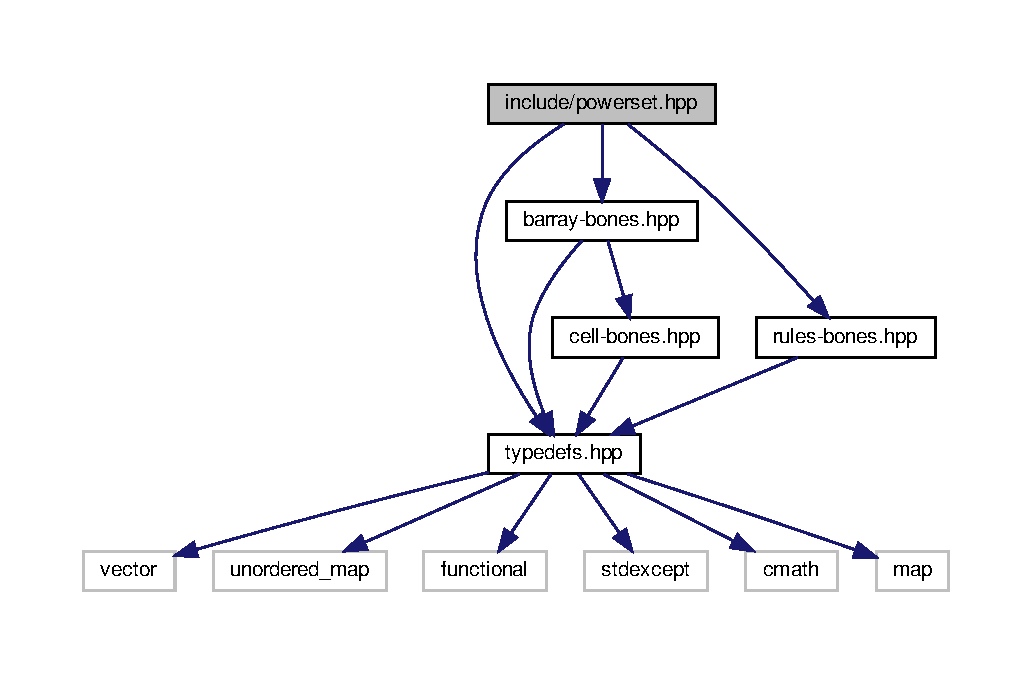
\includegraphics[width=350pt]{powerset_8hpp__incl}
\end{center}
\end{figure}
This graph shows which files directly or indirectly include this file\+:
\nopagebreak
\begin{figure}[H]
\begin{center}
\leavevmode
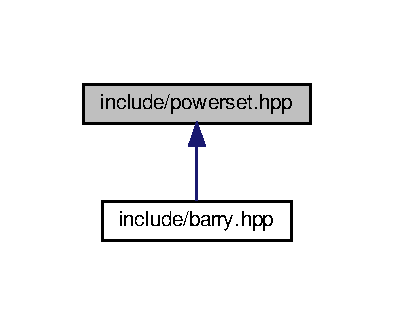
\includegraphics[width=189pt]{powerset_8hpp__dep__incl}
\end{center}
\end{figure}
\subsection*{Classes}
\begin{DoxyCompactItemize}
\item 
class \hyperlink{class_power_set}{Power\+Set$<$ Cell\+\_\+\+Type, Data\+\_\+\+Type $>$}
\end{DoxyCompactItemize}
\subsection*{Macros}
\begin{DoxyCompactItemize}
\item 
\#define \hyperlink{barry_8hpp_a707502c794083673439e006ba0646592}{L\+B\+A\+R\+R\+A\+Y\+\_\+\+P\+O\+W\+E\+R\+S\+E\+T\+\_\+\+H\+PP}~1
\end{DoxyCompactItemize}


\subsection{Macro Definition Documentation}
\mbox{\Hypertarget{barry_8hpp_a707502c794083673439e006ba0646592}\label{barry_8hpp_a707502c794083673439e006ba0646592}} 
\index{powerset.\+hpp@{powerset.\+hpp}!L\+B\+A\+R\+R\+A\+Y\+\_\+\+P\+O\+W\+E\+R\+S\+E\+T\+\_\+\+H\+PP@{L\+B\+A\+R\+R\+A\+Y\+\_\+\+P\+O\+W\+E\+R\+S\+E\+T\+\_\+\+H\+PP}}
\index{L\+B\+A\+R\+R\+A\+Y\+\_\+\+P\+O\+W\+E\+R\+S\+E\+T\+\_\+\+H\+PP@{L\+B\+A\+R\+R\+A\+Y\+\_\+\+P\+O\+W\+E\+R\+S\+E\+T\+\_\+\+H\+PP}!powerset.\+hpp@{powerset.\+hpp}}
\subsubsection{\texorpdfstring{L\+B\+A\+R\+R\+A\+Y\+\_\+\+P\+O\+W\+E\+R\+S\+E\+T\+\_\+\+H\+PP}{LBARRAY\_POWERSET\_HPP}}
{\footnotesize\ttfamily \#define L\+B\+A\+R\+R\+A\+Y\+\_\+\+P\+O\+W\+E\+R\+S\+E\+T\+\_\+\+H\+PP~1}



Definition at line 7 of file barry.\+hpp.


\hypertarget{statscounter_8hpp}{}\section{include/statscounter.hpp File Reference}
\label{statscounter_8hpp}\index{include/statscounter.\+hpp@{include/statscounter.\+hpp}}
{\ttfamily \#include \char`\"{}typedefs.\+hpp\char`\"{}}\newline
{\ttfamily \#include \char`\"{}barray-\/bones.\+hpp\char`\"{}}\newline
{\ttfamily \#include \char`\"{}statsdb.\+hpp\char`\"{}}\newline
{\ttfamily \#include \char`\"{}counters-\/bones.\+hpp\char`\"{}}\newline
Include dependency graph for statscounter.\+hpp\+:\nopagebreak
\begin{figure}[H]
\begin{center}
\leavevmode
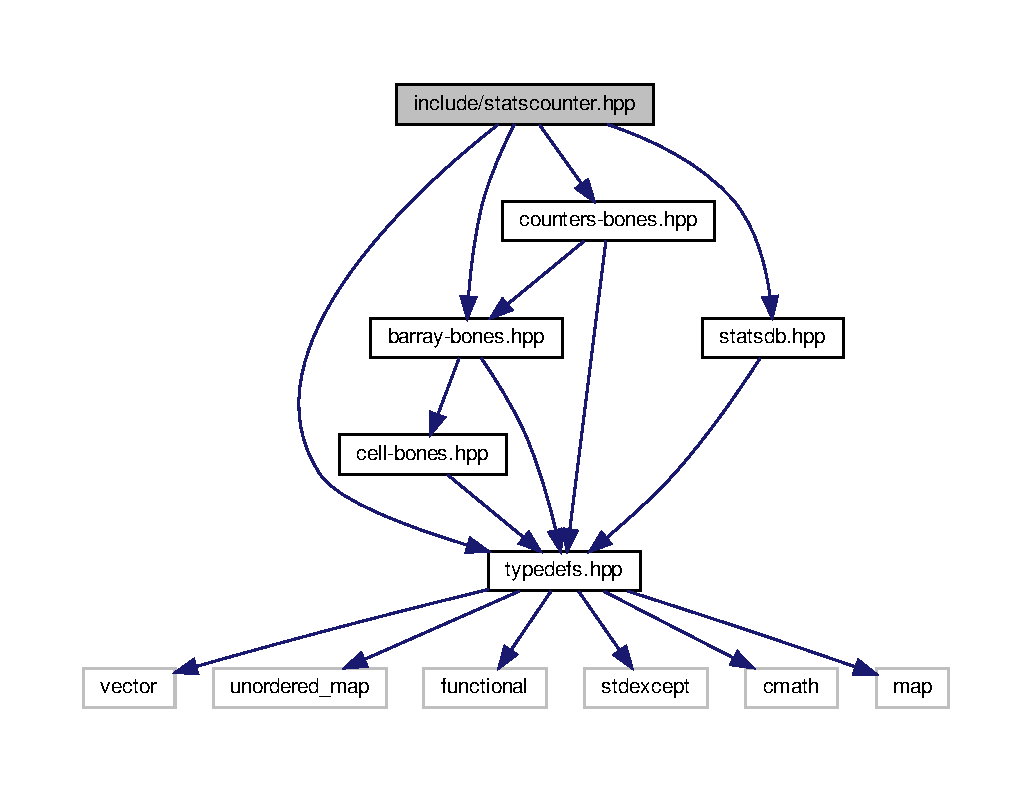
\includegraphics[width=342pt]{statscounter_8hpp__incl}
\end{center}
\end{figure}
This graph shows which files directly or indirectly include this file\+:\nopagebreak
\begin{figure}[H]
\begin{center}
\leavevmode
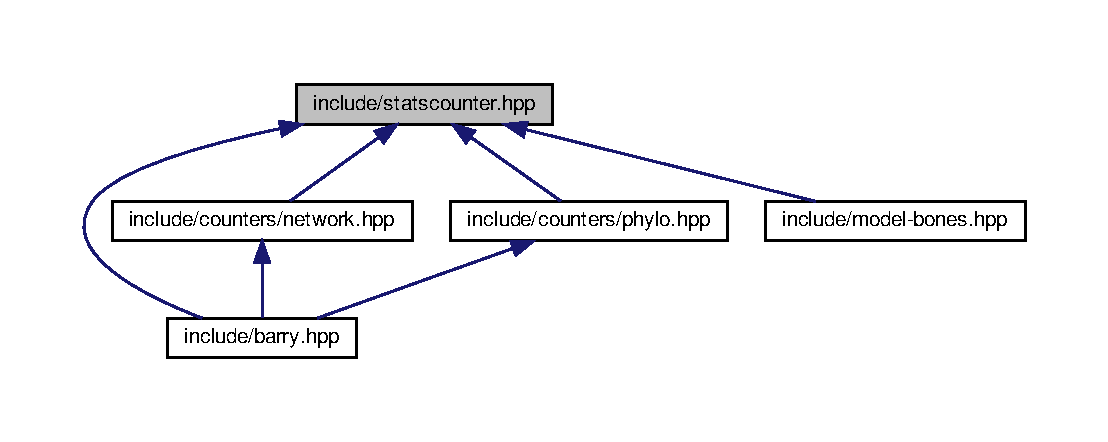
\includegraphics[width=203pt]{statscounter_8hpp__dep__incl}
\end{center}
\end{figure}
\subsection*{Classes}
\begin{DoxyCompactItemize}
\item 
class \hyperlink{class_stats_counter}{Stats\+Counter$<$ Array\+\_\+\+Type, Data\+\_\+\+Type $>$}
\begin{DoxyCompactList}\small\item\em Count stats for a single Array. \end{DoxyCompactList}\end{DoxyCompactItemize}
\subsection*{Macros}
\begin{DoxyCompactItemize}
\item 
\#define \hyperlink{barry_8hpp_a0eca09af8c8ad92a39bbc47492d97cf3}{S\+T\+A\+T\+S\+C\+O\+U\+N\+T\+E\+R\+\_\+\+H\+PP}~1
\item 
\#define \hyperlink{statscounter_8hpp_a0eca09af8c8ad92a39bbc47492d97cf3}{S\+T\+A\+T\+S\+C\+O\+U\+N\+T\+E\+R\+\_\+\+H\+PP}~1
\end{DoxyCompactItemize}


\subsection{Macro Definition Documentation}
\mbox{\Hypertarget{barry_8hpp_a0eca09af8c8ad92a39bbc47492d97cf3}\label{barry_8hpp_a0eca09af8c8ad92a39bbc47492d97cf3}} 
\index{statscounter.\+hpp@{statscounter.\+hpp}!S\+T\+A\+T\+S\+C\+O\+U\+N\+T\+E\+R\+\_\+\+H\+PP@{S\+T\+A\+T\+S\+C\+O\+U\+N\+T\+E\+R\+\_\+\+H\+PP}}
\index{S\+T\+A\+T\+S\+C\+O\+U\+N\+T\+E\+R\+\_\+\+H\+PP@{S\+T\+A\+T\+S\+C\+O\+U\+N\+T\+E\+R\+\_\+\+H\+PP}!statscounter.\+hpp@{statscounter.\+hpp}}
\subsubsection{\texorpdfstring{S\+T\+A\+T\+S\+C\+O\+U\+N\+T\+E\+R\+\_\+\+H\+PP}{STATSCOUNTER\_HPP}\hspace{0.1cm}{\footnotesize\ttfamily [1/2]}}
{\footnotesize\ttfamily \#define S\+T\+A\+T\+S\+C\+O\+U\+N\+T\+E\+R\+\_\+\+H\+PP~1}

\mbox{\Hypertarget{statscounter_8hpp_a0eca09af8c8ad92a39bbc47492d97cf3}\label{statscounter_8hpp_a0eca09af8c8ad92a39bbc47492d97cf3}} 
\index{statscounter.\+hpp@{statscounter.\+hpp}!S\+T\+A\+T\+S\+C\+O\+U\+N\+T\+E\+R\+\_\+\+H\+PP@{S\+T\+A\+T\+S\+C\+O\+U\+N\+T\+E\+R\+\_\+\+H\+PP}}
\index{S\+T\+A\+T\+S\+C\+O\+U\+N\+T\+E\+R\+\_\+\+H\+PP@{S\+T\+A\+T\+S\+C\+O\+U\+N\+T\+E\+R\+\_\+\+H\+PP}!statscounter.\+hpp@{statscounter.\+hpp}}
\subsubsection{\texorpdfstring{S\+T\+A\+T\+S\+C\+O\+U\+N\+T\+E\+R\+\_\+\+H\+PP}{STATSCOUNTER\_HPP}\hspace{0.1cm}{\footnotesize\ttfamily [2/2]}}
{\footnotesize\ttfamily \#define S\+T\+A\+T\+S\+C\+O\+U\+N\+T\+E\+R\+\_\+\+H\+PP~1}



Definition at line 9 of file statscounter.\+hpp.


\hypertarget{statsdb_8hpp}{}\section{include/statsdb.hpp File Reference}
\label{statsdb_8hpp}\index{include/statsdb.\+hpp@{include/statsdb.\+hpp}}
{\ttfamily \#include \char`\"{}typedefs.\+hpp\char`\"{}}\newline
Include dependency graph for statsdb.\+hpp\+:\nopagebreak
\begin{figure}[H]
\begin{center}
\leavevmode
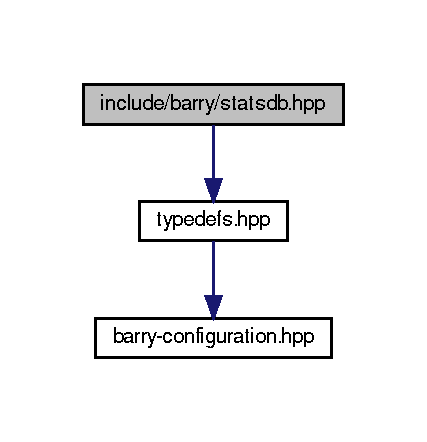
\includegraphics[width=181pt]{statsdb_8hpp__incl}
\end{center}
\end{figure}
This graph shows which files directly or indirectly include this file\+:
\nopagebreak
\begin{figure}[H]
\begin{center}
\leavevmode
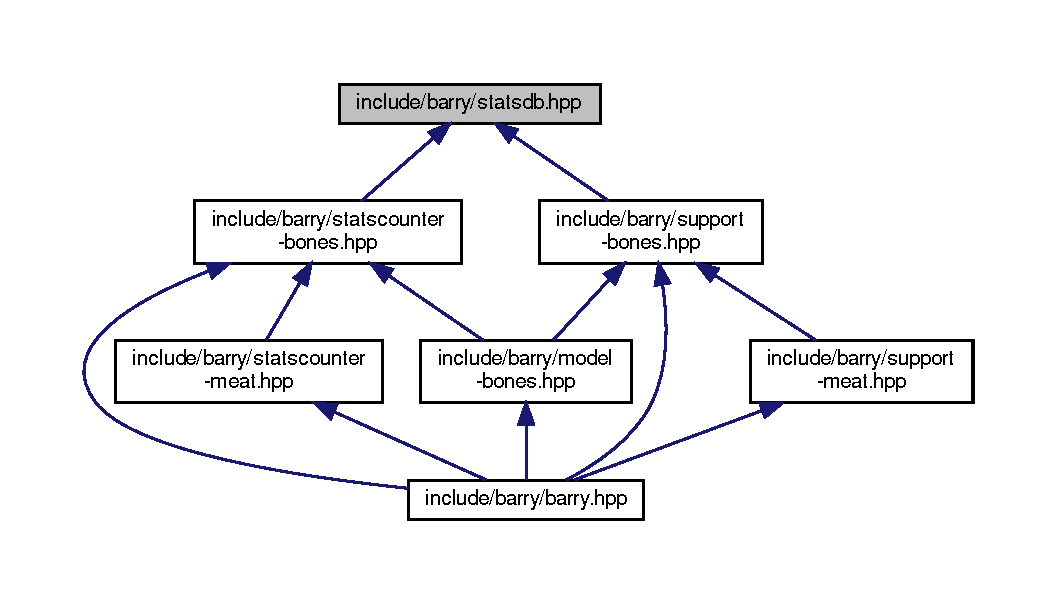
\includegraphics[width=350pt]{statsdb_8hpp__dep__incl}
\end{center}
\end{figure}
\subsection*{Classes}
\begin{DoxyCompactItemize}
\item 
struct \hyperlink{structvec_hasher}{vec\+Hasher$<$ T $>$}
\item 
class \hyperlink{class_stats_d_b}{Stats\+DB}
\begin{DoxyCompactList}\small\item\em Database of statistics. \end{DoxyCompactList}\end{DoxyCompactItemize}
\subsection*{Macros}
\begin{DoxyCompactItemize}
\item 
\#define \hyperlink{barry_8hpp_ab8b23226e678393ead26691f42ed6f58}{L\+B\+A\+R\+R\+A\+Y\+\_\+\+S\+T\+A\+T\+S\+D\+B\+\_\+\+H\+PP}~1
\end{DoxyCompactItemize}


\subsection{Macro Definition Documentation}
\mbox{\Hypertarget{barry_8hpp_ab8b23226e678393ead26691f42ed6f58}\label{barry_8hpp_ab8b23226e678393ead26691f42ed6f58}} 
\index{statsdb.\+hpp@{statsdb.\+hpp}!L\+B\+A\+R\+R\+A\+Y\+\_\+\+S\+T\+A\+T\+S\+D\+B\+\_\+\+H\+PP@{L\+B\+A\+R\+R\+A\+Y\+\_\+\+S\+T\+A\+T\+S\+D\+B\+\_\+\+H\+PP}}
\index{L\+B\+A\+R\+R\+A\+Y\+\_\+\+S\+T\+A\+T\+S\+D\+B\+\_\+\+H\+PP@{L\+B\+A\+R\+R\+A\+Y\+\_\+\+S\+T\+A\+T\+S\+D\+B\+\_\+\+H\+PP}!statsdb.\+hpp@{statsdb.\+hpp}}
\subsubsection{\texorpdfstring{L\+B\+A\+R\+R\+A\+Y\+\_\+\+S\+T\+A\+T\+S\+D\+B\+\_\+\+H\+PP}{LBARRAY\_STATSDB\_HPP}}
{\footnotesize\ttfamily \#define L\+B\+A\+R\+R\+A\+Y\+\_\+\+S\+T\+A\+T\+S\+D\+B\+\_\+\+H\+PP~1}



Definition at line 7 of file barry.\+hpp.


\hypertarget{support_8hpp}{}\section{include/support.hpp File Reference}
\label{support_8hpp}\index{include/support.\+hpp@{include/support.\+hpp}}
{\ttfamily \#include \char`\"{}typedefs.\+hpp\char`\"{}}\newline
{\ttfamily \#include \char`\"{}barray-\/bones.\+hpp\char`\"{}}\newline
{\ttfamily \#include \char`\"{}statsdb.\+hpp\char`\"{}}\newline
{\ttfamily \#include \char`\"{}counters-\/bones.\+hpp\char`\"{}}\newline
Include dependency graph for support.\+hpp\+:\nopagebreak
\begin{figure}[H]
\begin{center}
\leavevmode
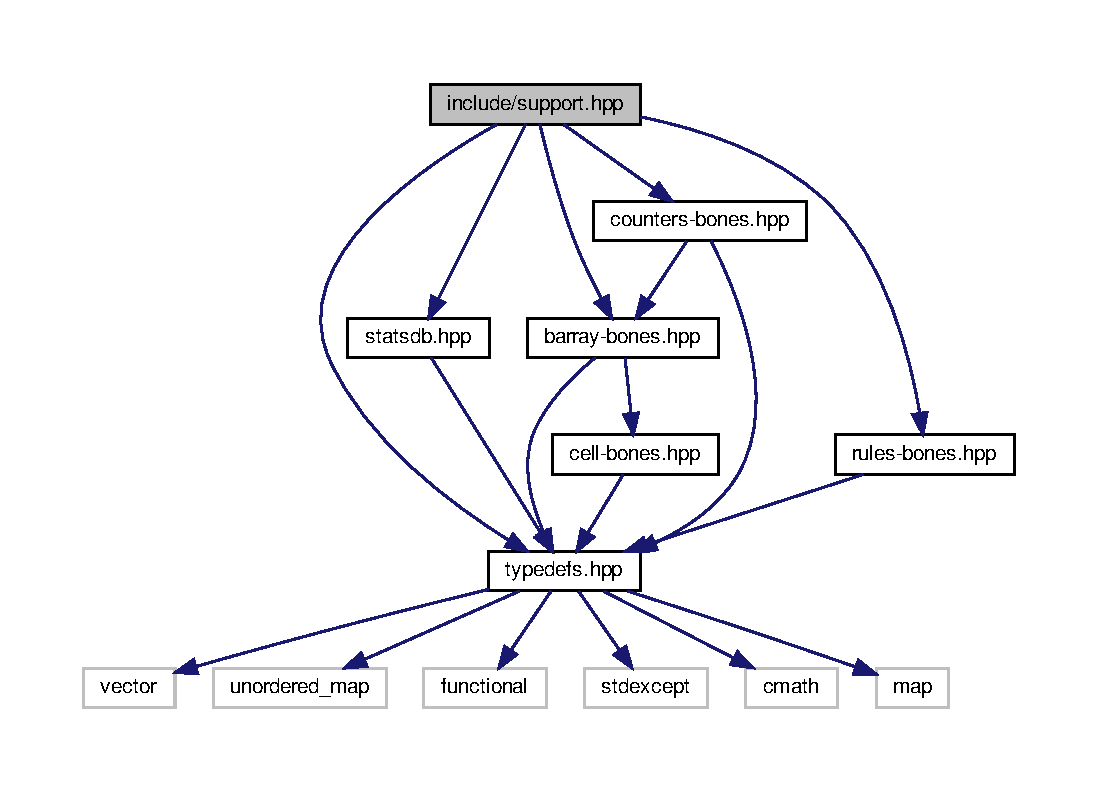
\includegraphics[width=350pt]{support_8hpp__incl}
\end{center}
\end{figure}
This graph shows which files directly or indirectly include this file\+:\nopagebreak
\begin{figure}[H]
\begin{center}
\leavevmode
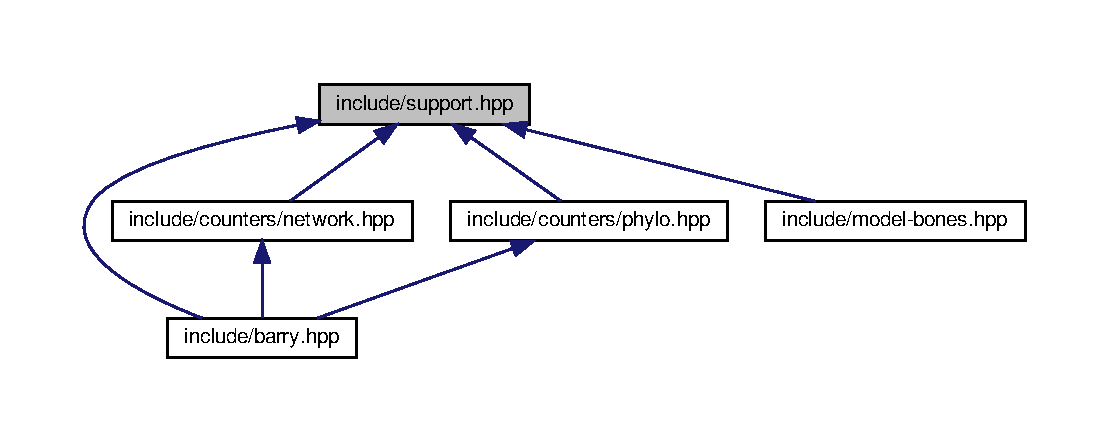
\includegraphics[width=350pt]{support_8hpp__dep__incl}
\end{center}
\end{figure}
\subsection*{Classes}
\begin{DoxyCompactItemize}
\item 
class \hyperlink{class_support}{Support$<$ Array\+\_\+\+Type, Data\+\_\+\+Type $>$}
\begin{DoxyCompactList}\small\item\em Compute the support of sufficient statistics. \end{DoxyCompactList}\end{DoxyCompactItemize}
\subsection*{Macros}
\begin{DoxyCompactItemize}
\item 
\#define \hyperlink{barry_8hpp_a318b14a3d775d872d85b9264e20b02dd}{S\+U\+P\+P\+O\+R\+T\+\_\+\+H\+PP}~1
\end{DoxyCompactItemize}


\subsection{Macro Definition Documentation}
\mbox{\Hypertarget{barry_8hpp_a318b14a3d775d872d85b9264e20b02dd}\label{barry_8hpp_a318b14a3d775d872d85b9264e20b02dd}} 
\index{support.\+hpp@{support.\+hpp}!S\+U\+P\+P\+O\+R\+T\+\_\+\+H\+PP@{S\+U\+P\+P\+O\+R\+T\+\_\+\+H\+PP}}
\index{S\+U\+P\+P\+O\+R\+T\+\_\+\+H\+PP@{S\+U\+P\+P\+O\+R\+T\+\_\+\+H\+PP}!support.\+hpp@{support.\+hpp}}
\subsubsection{\texorpdfstring{S\+U\+P\+P\+O\+R\+T\+\_\+\+H\+PP}{SUPPORT\_HPP}}
{\footnotesize\ttfamily \#define S\+U\+P\+P\+O\+R\+T\+\_\+\+H\+PP~1}



Definition at line 9 of file barry.\+hpp.


\hypertarget{typedefs_8hpp}{}\doxysection{include/barry/typedefs.hpp File Reference}
\label{typedefs_8hpp}\index{include/barry/typedefs.hpp@{include/barry/typedefs.hpp}}
{\ttfamily \#include \char`\"{}barry-\/configuration.\+hpp\char`\"{}}\newline
{\ttfamily \#include \char`\"{}barry-\/debug.\+hpp\char`\"{}}\newline
{\ttfamily \#include \char`\"{}progress.\+hpp\char`\"{}}\newline
Include dependency graph for typedefs.\+hpp\+:
\nopagebreak
\begin{figure}[H]
\begin{center}
\leavevmode
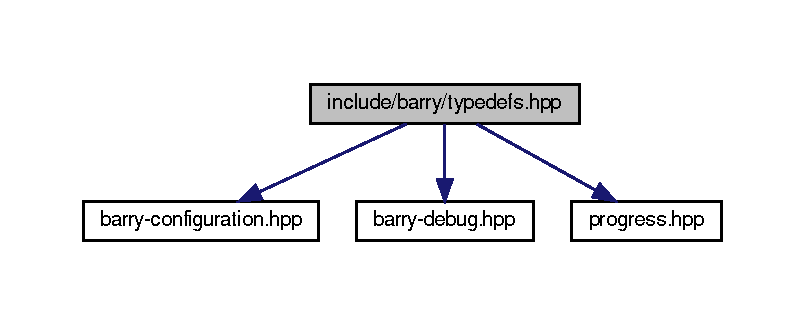
\includegraphics[width=350pt]{typedefs_8hpp__incl}
\end{center}
\end{figure}
This graph shows which files directly or indirectly include this file\+:
\nopagebreak
\begin{figure}[H]
\begin{center}
\leavevmode
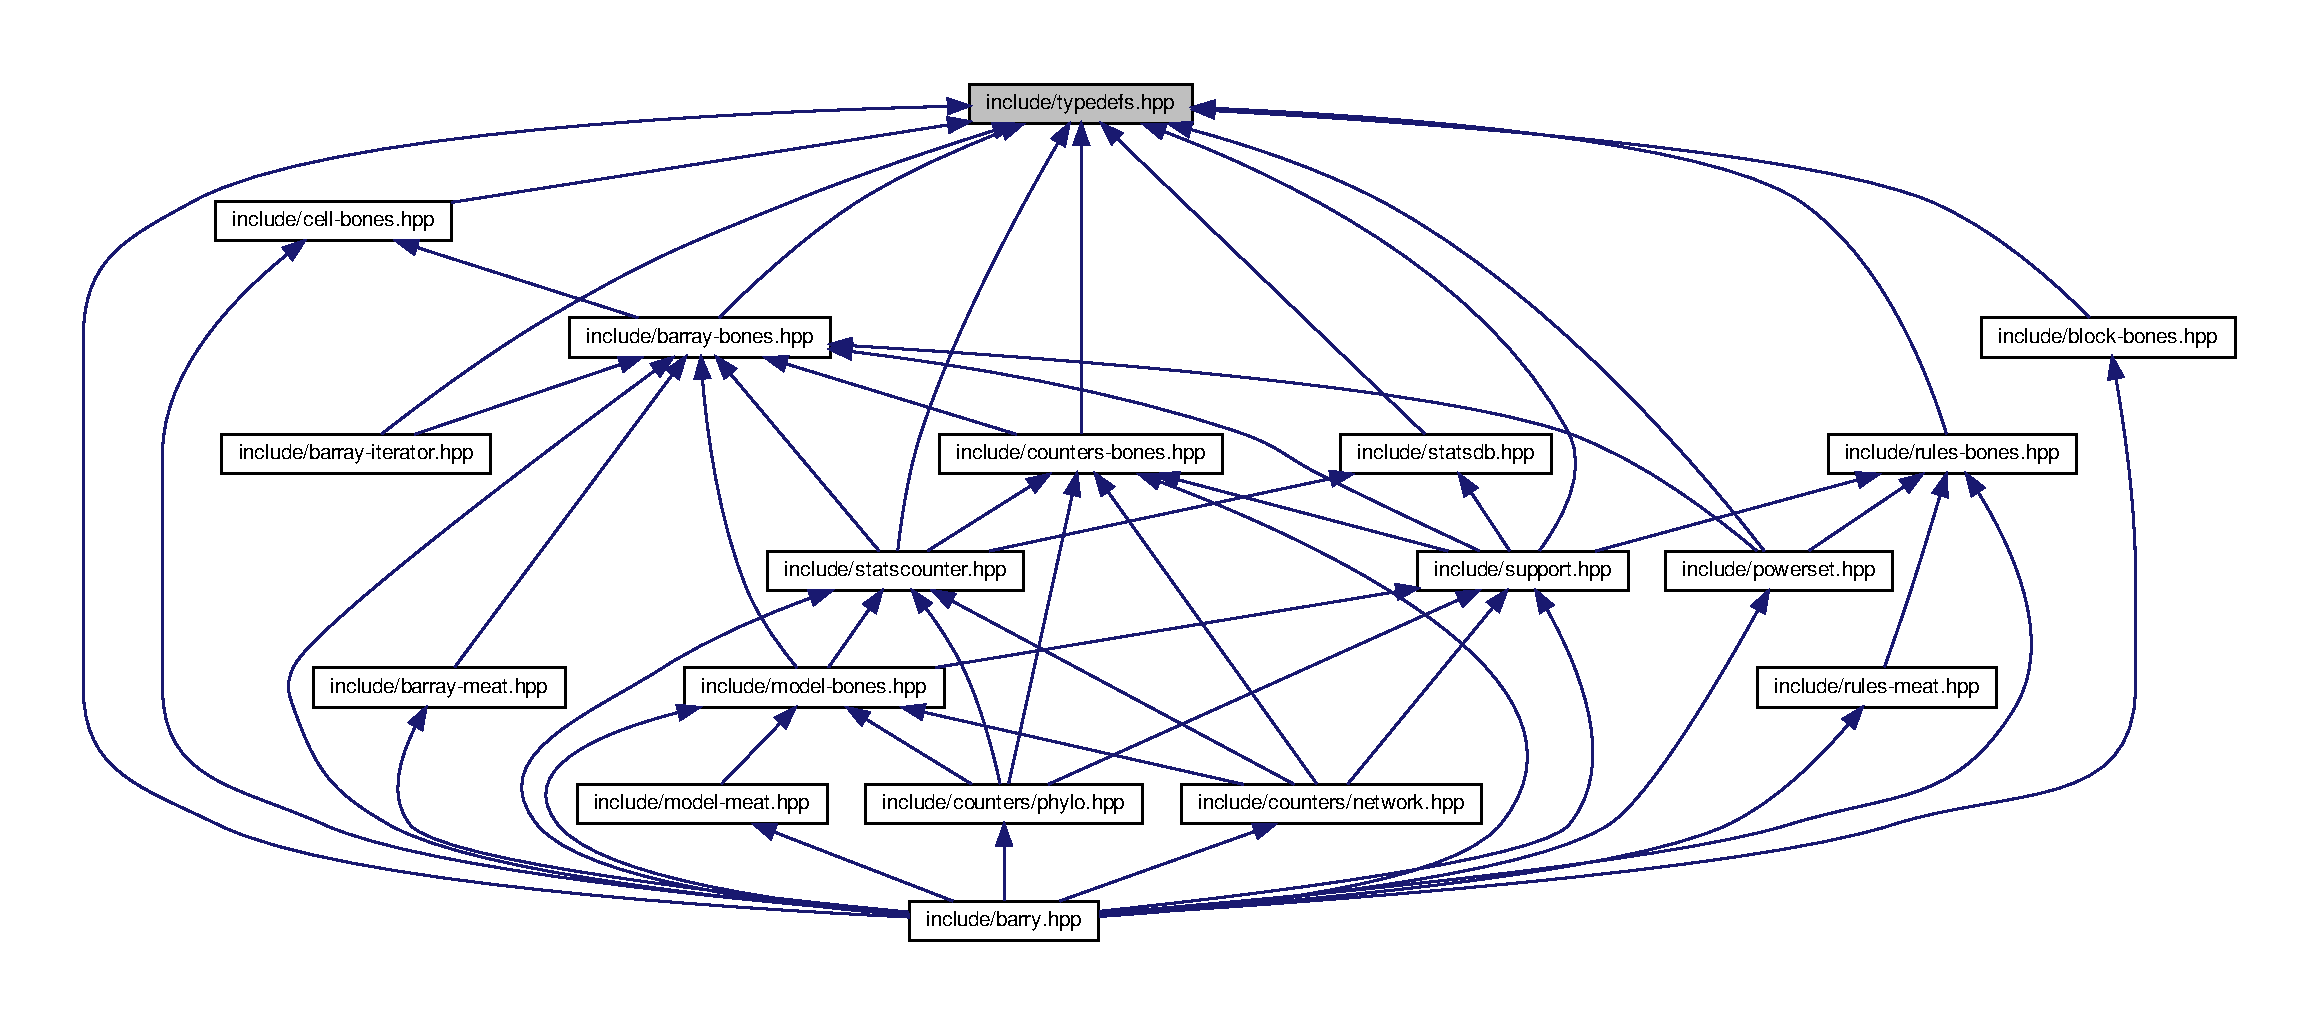
\includegraphics[width=209pt]{typedefs_8hpp__dep__incl}
\end{center}
\end{figure}
\doxysubsection*{Classes}
\begin{DoxyCompactItemize}
\item 
class \mbox{\hyperlink{class_entries}{Entries$<$ Cell\+\_\+\+Type $>$}}
\begin{DoxyCompactList}\small\item\em A wrapper class to store {\ttfamily source}, {\ttfamily target}, {\ttfamily val} from a {\ttfamily \mbox{\hyperlink{class_b_array}{BArray}}} object. \end{DoxyCompactList}\item 
struct \mbox{\hyperlink{structvec_hasher}{vec\+Hasher$<$ T $>$}}
\end{DoxyCompactItemize}
\doxysubsection*{Namespaces}
\begin{DoxyCompactItemize}
\item 
 \mbox{\hyperlink{namespace_c_h_e_c_k}{CHECK}}
\begin{DoxyCompactList}\small\item\em Integer constants used to specify which cell should be check. \end{DoxyCompactList}\item 
 \mbox{\hyperlink{namespace_e_x_i_s_t_s}{EXISTS}}
\begin{DoxyCompactList}\small\item\em Integer constants used to specify which cell should be check to exist or not. \end{DoxyCompactList}\end{DoxyCompactItemize}
\doxysubsection*{Typedefs}
\begin{DoxyCompactItemize}
\item 
typedef std\+::vector$<$ std\+::pair$<$ std\+::vector$<$ double $>$, size\+\_\+t $>$ $>$ \mbox{\hyperlink{typedefs_8hpp_a3aea7a9fde67a666803ef314b671b9b5}{Counts\+\_\+type}}
\item 
{\footnotesize template$<$typename Cell\+\_\+\+Type $>$ }\\using \mbox{\hyperlink{typedefs_8hpp_a84308a04a60581533b3c5e796c8248f5}{Row\+\_\+type}} = \mbox{\hyperlink{barry-configuration_8hpp_a1bb64c776ba5e9fc373665103b1a1772}{Map}}$<$ size\+\_\+t, \mbox{\hyperlink{class_cell}{Cell}}$<$ Cell\+\_\+\+Type $>$ $>$
\item 
{\footnotesize template$<$typename Cell\+\_\+\+Type $>$ }\\using \mbox{\hyperlink{typedefs_8hpp_adfb2ee3c0edfa46d47dc24cbbfabb11b}{Col\+\_\+type}} = \mbox{\hyperlink{barry-configuration_8hpp_a1bb64c776ba5e9fc373665103b1a1772}{Map}}$<$ size\+\_\+t, \mbox{\hyperlink{class_cell}{Cell}}$<$ Cell\+\_\+\+Type $>$ $\ast$ $>$
\item 
{\footnotesize template$<$typename Ta  = double, typename Tb  = size\+\_\+t$>$ }\\using \mbox{\hyperlink{typedefs_8hpp_a02ed8dec96bc528c8bc3d8cb3c4674a5}{Map\+Vec\+\_\+type}} = std\+::unordered\+\_\+map$<$ std\+::vector$<$ Ta $>$, Tb, \mbox{\hyperlink{structvec_hasher}{vec\+Hasher}}$<$ Ta $>$ $>$
\item 
{\footnotesize template$<$typename Array\+\_\+\+Type , typename Data\+\_\+\+Type $>$ }\\using \mbox{\hyperlink{typedefs_8hpp_aab7c9679e747e2f653246fbd03f26cc1}{Hasher\+\_\+fun\+\_\+type}} = std\+::function$<$ std\+::vector$<$ double $>$(const Array\+\_\+\+Type \&, Data\+\_\+\+Type $\ast$)$>$
\begin{DoxyCompactList}\small\item\em Hasher function used by the counter. \end{DoxyCompactList}\end{DoxyCompactItemize}
\textbf{ }\par
\begin{DoxyCompactItemize}
\item 
{\footnotesize template$<$typename Array\+\_\+\+Type , typename Data\+\_\+\+Type $>$ }\\using \mbox{\hyperlink{typedefs_8hpp_ad7626021d4acb1dfc9419e667923a01f}{Counter\+\_\+fun\+\_\+type}} = std\+::function$<$ double(const Array\+\_\+\+Type \&, size\+\_\+t, size\+\_\+t, Data\+\_\+\+Type \&)$>$
\begin{DoxyCompactList}\small\item\em \mbox{\hyperlink{class_counter}{Counter}} and rule functions. \end{DoxyCompactList}\item 
{\footnotesize template$<$typename Array\+\_\+\+Type , typename Data\+\_\+\+Type $>$ }\\using \mbox{\hyperlink{typedefs_8hpp_a940d68f006f1ffee7f5b207bf61aefe4}{Rule\+\_\+fun\+\_\+type}} = std\+::function$<$ bool(const Array\+\_\+\+Type \&, size\+\_\+t, size\+\_\+t, Data\+\_\+\+Type \&)$>$
\end{DoxyCompactItemize}

\doxysubsection*{Functions}
\begin{DoxyCompactItemize}
\item 
std\+::vector$<$ size\+\_\+t $>$ \mbox{\hyperlink{typedefs_8hpp_ab1d4f47a245caa5ee58da49231c054ca}{sort\+\_\+array}} (const double $\ast$v, size\+\_\+t start, size\+\_\+t ncols, size\+\_\+t nrows)
\begin{DoxyCompactList}\small\item\em Ascending sorting an array. \end{DoxyCompactList}\item 
{\footnotesize template$<$typename T $>$ }\\T \mbox{\hyperlink{typedefs_8hpp_ab9ddeecf87d68d3f44dd6a94b10aa786}{vec\+\_\+inner\+\_\+prod}} (const T $\ast$a, const T $\ast$b, size\+\_\+t n)
\item 
template$<$$>$ double \mbox{\hyperlink{typedefs_8hpp_af6f9c021aa2e49b1cb82fbd32026f1dc}{vec\+\_\+inner\+\_\+prod}} (const double $\ast$a, const double $\ast$b, size\+\_\+t n)
\end{DoxyCompactItemize}
\textbf{ }\par
\begin{DoxyCompactItemize}
\item 
{\footnotesize template$<$typename T $>$ }\\bool \mbox{\hyperlink{typedefs_8hpp_a0520b46efb182c4254e257ff5c5e7394}{vec\+\_\+equal}} (const std\+::vector$<$ T $>$ \&a, const std\+::vector$<$ T $>$ \&b)
\begin{DoxyCompactList}\small\item\em Compares if -\/a-\/ and -\/b-\/ are equal. \end{DoxyCompactList}\item 
{\footnotesize template$<$typename T $>$ }\\bool \mbox{\hyperlink{typedefs_8hpp_aed8ddfe5ae95bf4d6f76221ce06566fb}{vec\+\_\+equal\+\_\+approx}} (const std\+::vector$<$ T $>$ \&a, const std\+::vector$<$ T $>$ \&b, double eps=1e-\/100)
\end{DoxyCompactItemize}

\doxysubsection*{Variables}
\begin{DoxyCompactItemize}
\item 
const int \mbox{\hyperlink{namespace_c_h_e_c_k_a3acda1c74bfabb5b6b67e19d0ad2d52a}{CHECK\+::\+BOTH}} = -\/1
\item 
const int \mbox{\hyperlink{namespace_c_h_e_c_k_a35fad085a9d64167bd4550445c4dc9e1}{CHECK\+::\+NONE}} = 0
\item 
const int \mbox{\hyperlink{namespace_c_h_e_c_k_acf8ecf93ddfb75456112712630f8f722}{CHECK\+::\+ONE}} = 1
\item 
const int \mbox{\hyperlink{namespace_c_h_e_c_k_a2b112aaec4c59311376a5a60f291aa48}{CHECK\+::\+TWO}} = 2
\item 
const int \mbox{\hyperlink{namespace_e_x_i_s_t_s_a256db431572e1e7f26f8dfa6c9cae9bd}{EXISTS\+::\+BOTH}} = -\/1
\item 
const int \mbox{\hyperlink{namespace_e_x_i_s_t_s_a2f75d813424980b47f3e7c9608fb8416}{EXISTS\+::\+NONE}} = 0
\item 
const int \mbox{\hyperlink{namespace_e_x_i_s_t_s_a4c3717397d716d2bbd69d8239b3de033}{EXISTS\+::\+ONE}} = 1
\item 
const int \mbox{\hyperlink{namespace_e_x_i_s_t_s_ad76d02e8eb6d20715d333b72394b0648}{EXISTS\+::\+TWO}} = 1
\item 
const int \mbox{\hyperlink{namespace_e_x_i_s_t_s_a81eb362d951445c658942a433afddb97}{EXISTS\+::\+UKNOWN}} = -\/1
\item 
const int \mbox{\hyperlink{namespace_e_x_i_s_t_s_a03d550dd049f50f852b8fb4caa48238a}{EXISTS\+::\+AS\+\_\+\+ZERO}} = 0
\item 
const int \mbox{\hyperlink{namespace_e_x_i_s_t_s_a735e5ca6565905e84346e3ff62842a0a}{EXISTS\+::\+AS\+\_\+\+ONE}} = 1
\end{DoxyCompactItemize}


\doxysubsection{Typedef Documentation}
\mbox{\Hypertarget{typedefs_8hpp_adfb2ee3c0edfa46d47dc24cbbfabb11b}\label{typedefs_8hpp_adfb2ee3c0edfa46d47dc24cbbfabb11b}} 
\index{typedefs.hpp@{typedefs.hpp}!Col\_type@{Col\_type}}
\index{Col\_type@{Col\_type}!typedefs.hpp@{typedefs.hpp}}
\doxysubsubsection{\texorpdfstring{Col\_type}{Col\_type}}
{\footnotesize\ttfamily template$<$typename Cell\+\_\+\+Type $>$ \\
using \mbox{\hyperlink{typedefs_8hpp_adfb2ee3c0edfa46d47dc24cbbfabb11b}{Col\+\_\+type}} =  \mbox{\hyperlink{barry-configuration_8hpp_a1bb64c776ba5e9fc373665103b1a1772}{Map}}$<$ size\+\_\+t, \mbox{\hyperlink{class_cell}{Cell}}$<$Cell\+\_\+\+Type$>$$\ast$ $>$}



Definition at line 70 of file typedefs.\+hpp.

\mbox{\Hypertarget{typedefs_8hpp_ad7626021d4acb1dfc9419e667923a01f}\label{typedefs_8hpp_ad7626021d4acb1dfc9419e667923a01f}} 
\index{typedefs.hpp@{typedefs.hpp}!Counter\_fun\_type@{Counter\_fun\_type}}
\index{Counter\_fun\_type@{Counter\_fun\_type}!typedefs.hpp@{typedefs.hpp}}
\doxysubsubsection{\texorpdfstring{Counter\_fun\_type}{Counter\_fun\_type}}
{\footnotesize\ttfamily template$<$typename Array\+\_\+\+Type , typename Data\+\_\+\+Type $>$ \\
using \mbox{\hyperlink{typedefs_8hpp_ad7626021d4acb1dfc9419e667923a01f}{Counter\+\_\+fun\+\_\+type}} =  std\+::function$<$double(const Array\+\_\+\+Type \&, size\+\_\+t, size\+\_\+t, Data\+\_\+\+Type \&)$>$}



\mbox{\hyperlink{class_counter}{Counter}} and rule functions. 


\begin{DoxyParams}{Parameters}
{\em Array\+\_\+\+Type} & a \mbox{\hyperlink{class_b_array}{BArray}} \\
\hline
{\em unit,size\+\_\+t} & Focal cell \\
\hline
{\em Data\+\_\+\+Type} & Data associated with the function, for example, id of the attribute in the Array. \\
\hline
\end{DoxyParams}
\begin{DoxyReturn}{Returns}
{\ttfamily Counter\+\_\+fun\+\_\+type} a double (the change statistic) 

{\ttfamily Rule\+\_\+fun\+\_\+type} a bool. True if the cell is blocked. 
\end{DoxyReturn}


Definition at line 187 of file typedefs.\+hpp.

\mbox{\Hypertarget{typedefs_8hpp_a3aea7a9fde67a666803ef314b671b9b5}\label{typedefs_8hpp_a3aea7a9fde67a666803ef314b671b9b5}} 
\index{typedefs.hpp@{typedefs.hpp}!Counts\_type@{Counts\_type}}
\index{Counts\_type@{Counts\_type}!typedefs.hpp@{typedefs.hpp}}
\doxysubsubsection{\texorpdfstring{Counts\_type}{Counts\_type}}
{\footnotesize\ttfamily typedef std\+::vector$<$ std\+::pair$<$ std\+::vector$<$double$>$, size\+\_\+t $>$ $>$ \mbox{\hyperlink{typedefs_8hpp_a3aea7a9fde67a666803ef314b671b9b5}{Counts\+\_\+type}}}



Definition at line 51 of file typedefs.\+hpp.

\mbox{\Hypertarget{typedefs_8hpp_aab7c9679e747e2f653246fbd03f26cc1}\label{typedefs_8hpp_aab7c9679e747e2f653246fbd03f26cc1}} 
\index{typedefs.hpp@{typedefs.hpp}!Hasher\_fun\_type@{Hasher\_fun\_type}}
\index{Hasher\_fun\_type@{Hasher\_fun\_type}!typedefs.hpp@{typedefs.hpp}}
\doxysubsubsection{\texorpdfstring{Hasher\_fun\_type}{Hasher\_fun\_type}}
{\footnotesize\ttfamily template$<$typename Array\+\_\+\+Type , typename Data\+\_\+\+Type $>$ \\
using \mbox{\hyperlink{typedefs_8hpp_aab7c9679e747e2f653246fbd03f26cc1}{Hasher\+\_\+fun\+\_\+type}} =  std\+::function$<$std\+::vector$<$double$>$(const Array\+\_\+\+Type \&, Data\+\_\+\+Type $\ast$)$>$}



Hasher function used by the counter. 

Used to characterize the support of the array.


\begin{DoxyTemplParams}{Template Parameters}
{\em Array\+\_\+\+Type} & \\
\hline
\end{DoxyTemplParams}


Definition at line 200 of file typedefs.\+hpp.

\mbox{\Hypertarget{typedefs_8hpp_a02ed8dec96bc528c8bc3d8cb3c4674a5}\label{typedefs_8hpp_a02ed8dec96bc528c8bc3d8cb3c4674a5}} 
\index{typedefs.hpp@{typedefs.hpp}!MapVec\_type@{MapVec\_type}}
\index{MapVec\_type@{MapVec\_type}!typedefs.hpp@{typedefs.hpp}}
\doxysubsubsection{\texorpdfstring{MapVec\_type}{MapVec\_type}}
{\footnotesize\ttfamily template$<$typename Ta  = double, typename Tb  = size\+\_\+t$>$ \\
using \mbox{\hyperlink{typedefs_8hpp_a02ed8dec96bc528c8bc3d8cb3c4674a5}{Map\+Vec\+\_\+type}} =  std\+::unordered\+\_\+map$<$ std\+::vector$<$ Ta $>$, Tb, \mbox{\hyperlink{structvec_hasher}{vec\+Hasher}}$<$Ta$>$ $>$}



Definition at line 128 of file typedefs.\+hpp.

\mbox{\Hypertarget{typedefs_8hpp_a84308a04a60581533b3c5e796c8248f5}\label{typedefs_8hpp_a84308a04a60581533b3c5e796c8248f5}} 
\index{typedefs.hpp@{typedefs.hpp}!Row\_type@{Row\_type}}
\index{Row\_type@{Row\_type}!typedefs.hpp@{typedefs.hpp}}
\doxysubsubsection{\texorpdfstring{Row\_type}{Row\_type}}
{\footnotesize\ttfamily template$<$typename Cell\+\_\+\+Type $>$ \\
using \mbox{\hyperlink{typedefs_8hpp_a84308a04a60581533b3c5e796c8248f5}{Row\+\_\+type}} =  \mbox{\hyperlink{barry-configuration_8hpp_a1bb64c776ba5e9fc373665103b1a1772}{Map}}$<$ size\+\_\+t, \mbox{\hyperlink{class_cell}{Cell}}$<$Cell\+\_\+\+Type$>$ $>$}



Definition at line 67 of file typedefs.\+hpp.

\mbox{\Hypertarget{typedefs_8hpp_a940d68f006f1ffee7f5b207bf61aefe4}\label{typedefs_8hpp_a940d68f006f1ffee7f5b207bf61aefe4}} 
\index{typedefs.hpp@{typedefs.hpp}!Rule\_fun\_type@{Rule\_fun\_type}}
\index{Rule\_fun\_type@{Rule\_fun\_type}!typedefs.hpp@{typedefs.hpp}}
\doxysubsubsection{\texorpdfstring{Rule\_fun\_type}{Rule\_fun\_type}}
{\footnotesize\ttfamily template$<$typename Array\+\_\+\+Type , typename Data\+\_\+\+Type $>$ \\
using \mbox{\hyperlink{typedefs_8hpp_a940d68f006f1ffee7f5b207bf61aefe4}{Rule\+\_\+fun\+\_\+type}} =  std\+::function$<$bool(const Array\+\_\+\+Type \&, size\+\_\+t, size\+\_\+t, Data\+\_\+\+Type \&)$>$}



Definition at line 190 of file typedefs.\+hpp.



\doxysubsection{Function Documentation}
\mbox{\Hypertarget{typedefs_8hpp_ab1d4f47a245caa5ee58da49231c054ca}\label{typedefs_8hpp_ab1d4f47a245caa5ee58da49231c054ca}} 
\index{typedefs.hpp@{typedefs.hpp}!sort\_array@{sort\_array}}
\index{sort\_array@{sort\_array}!typedefs.hpp@{typedefs.hpp}}
\doxysubsubsection{\texorpdfstring{sort\_array()}{sort\_array()}}
{\footnotesize\ttfamily std\+::vector$<$ size\+\_\+t $>$ sort\+\_\+array (\begin{DoxyParamCaption}\item[{const double $\ast$}]{v,  }\item[{size\+\_\+t}]{start,  }\item[{size\+\_\+t}]{ncols,  }\item[{size\+\_\+t}]{nrows }\end{DoxyParamCaption})\hspace{0.3cm}{\ttfamily [inline]}}



Ascending sorting an array. 

It will sort an array solving ties using the next column. Data is stored column-\/wise.


\begin{DoxyTemplParams}{Template Parameters}
{\em T} & \\
\hline
\end{DoxyTemplParams}

\begin{DoxyParams}{Parameters}
{\em v} & \\
\hline
{\em nrows} & \\
\hline
\end{DoxyParams}
\begin{DoxyReturn}{Returns}
std\+::vector$<$size\+\_\+t$>$ The sorting index. 
\end{DoxyReturn}


Definition at line 141 of file typedefs.\+hpp.

\mbox{\Hypertarget{typedefs_8hpp_a0520b46efb182c4254e257ff5c5e7394}\label{typedefs_8hpp_a0520b46efb182c4254e257ff5c5e7394}} 
\index{typedefs.hpp@{typedefs.hpp}!vec\_equal@{vec\_equal}}
\index{vec\_equal@{vec\_equal}!typedefs.hpp@{typedefs.hpp}}
\doxysubsubsection{\texorpdfstring{vec\_equal()}{vec\_equal()}}
{\footnotesize\ttfamily template$<$typename T $>$ \\
bool vec\+\_\+equal (\begin{DoxyParamCaption}\item[{const std\+::vector$<$ T $>$ \&}]{a,  }\item[{const std\+::vector$<$ T $>$ \&}]{b }\end{DoxyParamCaption})\hspace{0.3cm}{\ttfamily [inline]}}



Compares if -\/a-\/ and -\/b-\/ are equal. 


\begin{DoxyParams}{Parameters}
{\em a,b} & Two vectors of the same length \\
\hline
\end{DoxyParams}
\begin{DoxyReturn}{Returns}
{\ttfamily true} if all elements are equal. 
\end{DoxyReturn}


Definition at line 210 of file typedefs.\+hpp.

\mbox{\Hypertarget{typedefs_8hpp_aed8ddfe5ae95bf4d6f76221ce06566fb}\label{typedefs_8hpp_aed8ddfe5ae95bf4d6f76221ce06566fb}} 
\index{typedefs.hpp@{typedefs.hpp}!vec\_equal\_approx@{vec\_equal\_approx}}
\index{vec\_equal\_approx@{vec\_equal\_approx}!typedefs.hpp@{typedefs.hpp}}
\doxysubsubsection{\texorpdfstring{vec\_equal\_approx()}{vec\_equal\_approx()}}
{\footnotesize\ttfamily template$<$typename T $>$ \\
bool vec\+\_\+equal\+\_\+approx (\begin{DoxyParamCaption}\item[{const std\+::vector$<$ T $>$ \&}]{a,  }\item[{const std\+::vector$<$ T $>$ \&}]{b,  }\item[{double}]{eps = {\ttfamily 1e-\/100} }\end{DoxyParamCaption})\hspace{0.3cm}{\ttfamily [inline]}}



Definition at line 235 of file typedefs.\+hpp.

\mbox{\Hypertarget{typedefs_8hpp_af6f9c021aa2e49b1cb82fbd32026f1dc}\label{typedefs_8hpp_af6f9c021aa2e49b1cb82fbd32026f1dc}} 
\index{typedefs.hpp@{typedefs.hpp}!vec\_inner\_prod@{vec\_inner\_prod}}
\index{vec\_inner\_prod@{vec\_inner\_prod}!typedefs.hpp@{typedefs.hpp}}
\doxysubsubsection{\texorpdfstring{vec\_inner\_prod()}{vec\_inner\_prod()}\hspace{0.1cm}{\footnotesize\ttfamily [1/2]}}
{\footnotesize\ttfamily template$<$$>$ \\
double vec\+\_\+inner\+\_\+prod (\begin{DoxyParamCaption}\item[{const double $\ast$}]{a,  }\item[{const double $\ast$}]{b,  }\item[{size\+\_\+t}]{n }\end{DoxyParamCaption})\hspace{0.3cm}{\ttfamily [inline]}}



Definition at line 286 of file typedefs.\+hpp.

\mbox{\Hypertarget{typedefs_8hpp_ab9ddeecf87d68d3f44dd6a94b10aa786}\label{typedefs_8hpp_ab9ddeecf87d68d3f44dd6a94b10aa786}} 
\index{typedefs.hpp@{typedefs.hpp}!vec\_inner\_prod@{vec\_inner\_prod}}
\index{vec\_inner\_prod@{vec\_inner\_prod}!typedefs.hpp@{typedefs.hpp}}
\doxysubsubsection{\texorpdfstring{vec\_inner\_prod()}{vec\_inner\_prod()}\hspace{0.1cm}{\footnotesize\ttfamily [2/2]}}
{\footnotesize\ttfamily template$<$typename T $>$ \\
T vec\+\_\+inner\+\_\+prod (\begin{DoxyParamCaption}\item[{const T $\ast$}]{a,  }\item[{const T $\ast$}]{b,  }\item[{size\+\_\+t}]{n }\end{DoxyParamCaption})\hspace{0.3cm}{\ttfamily [inline]}}



Definition at line 263 of file typedefs.\+hpp.


\hypertarget{vectors_8hpp}{}\section{include/barry/vectors.hpp File Reference}
\label{vectors_8hpp}\index{include/barry/vectors.\+hpp@{include/barry/vectors.\+hpp}}
{\ttfamily \#include $<$vector$>$}\newline
Include dependency graph for vectors.\+hpp\+:
\nopagebreak
\begin{figure}[H]
\begin{center}
\leavevmode
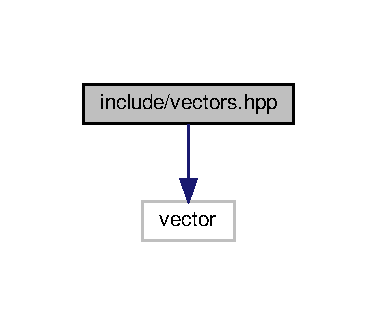
\includegraphics[width=206pt]{vectors_8hpp__incl}
\end{center}
\end{figure}
\subsection*{Functions}
\begin{DoxyCompactItemize}
\item 
{\footnotesize template$<$typename T $>$ }\\bool \hyperlink{vectors_8hpp_a0520b46efb182c4254e257ff5c5e7394}{vec\+\_\+equal} (const std\+::vector$<$ T $>$ \&a, const std\+::vector$<$ T $>$ \&b)
\begin{DoxyCompactList}\small\item\em Compares if -\/a-\/ and -\/b-\/ are equal. \end{DoxyCompactList}\end{DoxyCompactItemize}


\subsection{Function Documentation}
\mbox{\Hypertarget{vectors_8hpp_a0520b46efb182c4254e257ff5c5e7394}\label{vectors_8hpp_a0520b46efb182c4254e257ff5c5e7394}} 
\index{vectors.\+hpp@{vectors.\+hpp}!vec\+\_\+equal@{vec\+\_\+equal}}
\index{vec\+\_\+equal@{vec\+\_\+equal}!vectors.\+hpp@{vectors.\+hpp}}
\subsubsection{\texorpdfstring{vec\+\_\+equal()}{vec\_equal()}}
{\footnotesize\ttfamily template$<$typename T $>$ \\
bool vec\+\_\+equal (\begin{DoxyParamCaption}\item[{const std\+::vector$<$ T $>$ \&}]{a,  }\item[{const std\+::vector$<$ T $>$ \&}]{b }\end{DoxyParamCaption})\hspace{0.3cm}{\ttfamily [inline]}}



Compares if -\/a-\/ and -\/b-\/ are equal. 


\begin{DoxyParams}{Parameters}
{\em a,b} & Two vectors of the same length \\
\hline
\end{DoxyParams}
\begin{DoxyReturn}{Returns}
{\ttfamily true} if all elements are equal. 
\end{DoxyReturn}


Definition at line 11 of file vectors.\+hpp.


\hypertarget{_r_e_a_d_m_e_8md}{}\doxysection{README.\+md File Reference}
\label{_r_e_a_d_m_e_8md}\index{README.md@{README.md}}

%--- End generated contents ---

% Index
\backmatter
\newpage
\phantomsection
\clearemptydoublepage
\addcontentsline{toc}{chapter}{Index}
\printindex

\end{document}
